% Options for packages loaded elsewhere
\PassOptionsToPackage{unicode}{hyperref}
\PassOptionsToPackage{hyphens}{url}
\PassOptionsToPackage{dvipsnames,svgnames,x11names}{xcolor}
%
\documentclass[
  letterpaper,
  DIV=11,
  numbers=noendperiod]{scrreprt}

\usepackage{amsmath,amssymb}
\usepackage{iftex}
\ifPDFTeX
  \usepackage[T1]{fontenc}
  \usepackage[utf8]{inputenc}
  \usepackage{textcomp} % provide euro and other symbols
\else % if luatex or xetex
  \usepackage{unicode-math}
  \defaultfontfeatures{Scale=MatchLowercase}
  \defaultfontfeatures[\rmfamily]{Ligatures=TeX,Scale=1}
\fi
\usepackage{lmodern}
\ifPDFTeX\else  
    % xetex/luatex font selection
\fi
% Use upquote if available, for straight quotes in verbatim environments
\IfFileExists{upquote.sty}{\usepackage{upquote}}{}
\IfFileExists{microtype.sty}{% use microtype if available
  \usepackage[]{microtype}
  \UseMicrotypeSet[protrusion]{basicmath} % disable protrusion for tt fonts
}{}
\makeatletter
\@ifundefined{KOMAClassName}{% if non-KOMA class
  \IfFileExists{parskip.sty}{%
    \usepackage{parskip}
  }{% else
    \setlength{\parindent}{0pt}
    \setlength{\parskip}{6pt plus 2pt minus 1pt}}
}{% if KOMA class
  \KOMAoptions{parskip=half}}
\makeatother
\usepackage{xcolor}
\usepackage{svg}
\setlength{\emergencystretch}{3em} % prevent overfull lines
\setcounter{secnumdepth}{5}
% Make \paragraph and \subparagraph free-standing
\ifx\paragraph\undefined\else
  \let\oldparagraph\paragraph
  \renewcommand{\paragraph}[1]{\oldparagraph{#1}\mbox{}}
\fi
\ifx\subparagraph\undefined\else
  \let\oldsubparagraph\subparagraph
  \renewcommand{\subparagraph}[1]{\oldsubparagraph{#1}\mbox{}}
\fi

\usepackage{color}
\usepackage{fancyvrb}
\newcommand{\VerbBar}{|}
\newcommand{\VERB}{\Verb[commandchars=\\\{\}]}
\DefineVerbatimEnvironment{Highlighting}{Verbatim}{commandchars=\\\{\}}
% Add ',fontsize=\small' for more characters per line
\newenvironment{Shaded}{}{}
\newcommand{\AlertTok}[1]{\textcolor[rgb]{1.00,0.33,0.33}{\textbf{#1}}}
\newcommand{\AnnotationTok}[1]{\textcolor[rgb]{0.42,0.45,0.49}{#1}}
\newcommand{\AttributeTok}[1]{\textcolor[rgb]{0.84,0.23,0.29}{#1}}
\newcommand{\BaseNTok}[1]{\textcolor[rgb]{0.00,0.36,0.77}{#1}}
\newcommand{\BuiltInTok}[1]{\textcolor[rgb]{0.84,0.23,0.29}{#1}}
\newcommand{\CharTok}[1]{\textcolor[rgb]{0.01,0.18,0.38}{#1}}
\newcommand{\CommentTok}[1]{\textcolor[rgb]{0.42,0.45,0.49}{#1}}
\newcommand{\CommentVarTok}[1]{\textcolor[rgb]{0.42,0.45,0.49}{#1}}
\newcommand{\ConstantTok}[1]{\textcolor[rgb]{0.00,0.36,0.77}{#1}}
\newcommand{\ControlFlowTok}[1]{\textcolor[rgb]{0.84,0.23,0.29}{#1}}
\newcommand{\DataTypeTok}[1]{\textcolor[rgb]{0.84,0.23,0.29}{#1}}
\newcommand{\DecValTok}[1]{\textcolor[rgb]{0.00,0.36,0.77}{#1}}
\newcommand{\DocumentationTok}[1]{\textcolor[rgb]{0.42,0.45,0.49}{#1}}
\newcommand{\ErrorTok}[1]{\textcolor[rgb]{1.00,0.33,0.33}{\underline{#1}}}
\newcommand{\ExtensionTok}[1]{\textcolor[rgb]{0.84,0.23,0.29}{\textbf{#1}}}
\newcommand{\FloatTok}[1]{\textcolor[rgb]{0.00,0.36,0.77}{#1}}
\newcommand{\FunctionTok}[1]{\textcolor[rgb]{0.44,0.26,0.76}{#1}}
\newcommand{\ImportTok}[1]{\textcolor[rgb]{0.01,0.18,0.38}{#1}}
\newcommand{\InformationTok}[1]{\textcolor[rgb]{0.42,0.45,0.49}{#1}}
\newcommand{\KeywordTok}[1]{\textcolor[rgb]{0.84,0.23,0.29}{#1}}
\newcommand{\NormalTok}[1]{\textcolor[rgb]{0.14,0.16,0.18}{#1}}
\newcommand{\OperatorTok}[1]{\textcolor[rgb]{0.14,0.16,0.18}{#1}}
\newcommand{\OtherTok}[1]{\textcolor[rgb]{0.44,0.26,0.76}{#1}}
\newcommand{\PreprocessorTok}[1]{\textcolor[rgb]{0.84,0.23,0.29}{#1}}
\newcommand{\RegionMarkerTok}[1]{\textcolor[rgb]{0.42,0.45,0.49}{#1}}
\newcommand{\SpecialCharTok}[1]{\textcolor[rgb]{0.00,0.36,0.77}{#1}}
\newcommand{\SpecialStringTok}[1]{\textcolor[rgb]{0.01,0.18,0.38}{#1}}
\newcommand{\StringTok}[1]{\textcolor[rgb]{0.01,0.18,0.38}{#1}}
\newcommand{\VariableTok}[1]{\textcolor[rgb]{0.89,0.38,0.04}{#1}}
\newcommand{\VerbatimStringTok}[1]{\textcolor[rgb]{0.01,0.18,0.38}{#1}}
\newcommand{\WarningTok}[1]{\textcolor[rgb]{1.00,0.33,0.33}{#1}}

\providecommand{\tightlist}{%
  \setlength{\itemsep}{0pt}\setlength{\parskip}{0pt}}\usepackage{longtable,booktabs,array}
\usepackage{multirow}
\usepackage{calc} % for calculating minipage widths
% Correct order of tables after \paragraph or \subparagraph
\usepackage{etoolbox}
\makeatletter
\patchcmd\longtable{\par}{\if@noskipsec\mbox{}\fi\par}{}{}
\makeatother
% Allow footnotes in longtable head/foot
\IfFileExists{footnotehyper.sty}{\usepackage{footnotehyper}}{\usepackage{footnote}}
\makesavenoteenv{longtable}
\usepackage{graphicx}
\makeatletter
\def\maxwidth{\ifdim\Gin@nat@width>\linewidth\linewidth\else\Gin@nat@width\fi}
\def\maxheight{\ifdim\Gin@nat@height>\textheight\textheight\else\Gin@nat@height\fi}
\makeatother
% Scale images if necessary, so that they will not overflow the page
% margins by default, and it is still possible to overwrite the defaults
% using explicit options in \includegraphics[width, height, ...]{}
\setkeys{Gin}{width=\maxwidth,height=\maxheight,keepaspectratio}
% Set default figure placement to htbp
\makeatletter
\def\fps@figure{htbp}
\makeatother
% definitions for citeproc citations
\NewDocumentCommand\citeproctext{}{}
\NewDocumentCommand\citeproc{mm}{%
  \begingroup\def\citeproctext{#2}\cite{#1}\endgroup}
\makeatletter
 % allow citations to break across lines
 \let\@cite@ofmt\@firstofone
 % avoid brackets around text for \cite:
 \def\@biblabel#1{}
 \def\@cite#1#2{{#1\if@tempswa , #2\fi}}
\makeatother
\newlength{\cslhangindent}
\setlength{\cslhangindent}{1.5em}
\newlength{\csllabelwidth}
\setlength{\csllabelwidth}{3em}
\newenvironment{CSLReferences}[2] % #1 hanging-indent, #2 entry-spacing
 {\begin{list}{}{%
  \setlength{\itemindent}{0pt}
  \setlength{\leftmargin}{0pt}
  \setlength{\parsep}{0pt}
  % turn on hanging indent if param 1 is 1
  \ifodd #1
   \setlength{\leftmargin}{\cslhangindent}
   \setlength{\itemindent}{-1\cslhangindent}
  \fi
  % set entry spacing
  \setlength{\itemsep}{#2\baselineskip}}}
 {\end{list}}
\usepackage{calc}
\newcommand{\CSLBlock}[1]{\hfill\break\parbox[t]{\linewidth}{\strut\ignorespaces#1\strut}}
\newcommand{\CSLLeftMargin}[1]{\parbox[t]{\csllabelwidth}{\strut#1\strut}}
\newcommand{\CSLRightInline}[1]{\parbox[t]{\linewidth - \csllabelwidth}{\strut#1\strut}}
\newcommand{\CSLIndent}[1]{\hspace{\cslhangindent}#1}

\KOMAoption{captions}{tableheading}
\makeatletter
\@ifpackageloaded{tcolorbox}{}{\usepackage[skins,breakable]{tcolorbox}}
\@ifpackageloaded{fontawesome5}{}{\usepackage{fontawesome5}}
\definecolor{quarto-callout-color}{HTML}{909090}
\definecolor{quarto-callout-note-color}{HTML}{0758E5}
\definecolor{quarto-callout-important-color}{HTML}{CC1914}
\definecolor{quarto-callout-warning-color}{HTML}{EB9113}
\definecolor{quarto-callout-tip-color}{HTML}{00A047}
\definecolor{quarto-callout-caution-color}{HTML}{FC5300}
\definecolor{quarto-callout-color-frame}{HTML}{acacac}
\definecolor{quarto-callout-note-color-frame}{HTML}{4582ec}
\definecolor{quarto-callout-important-color-frame}{HTML}{d9534f}
\definecolor{quarto-callout-warning-color-frame}{HTML}{f0ad4e}
\definecolor{quarto-callout-tip-color-frame}{HTML}{02b875}
\definecolor{quarto-callout-caution-color-frame}{HTML}{fd7e14}
\makeatother
\makeatletter
\@ifpackageloaded{bookmark}{}{\usepackage{bookmark}}
\makeatother
\makeatletter
\@ifpackageloaded{caption}{}{\usepackage{caption}}
\AtBeginDocument{%
\ifdefined\contentsname
  \renewcommand*\contentsname{Table of contents}
\else
  \newcommand\contentsname{Table of contents}
\fi
\ifdefined\listfigurename
  \renewcommand*\listfigurename{List of Figures}
\else
  \newcommand\listfigurename{List of Figures}
\fi
\ifdefined\listtablename
  \renewcommand*\listtablename{List of Tables}
\else
  \newcommand\listtablename{List of Tables}
\fi
\ifdefined\figurename
  \renewcommand*\figurename{Figure}
\else
  \newcommand\figurename{Figure}
\fi
\ifdefined\tablename
  \renewcommand*\tablename{Table}
\else
  \newcommand\tablename{Table}
\fi
}
\@ifpackageloaded{float}{}{\usepackage{float}}
\floatstyle{ruled}
\@ifundefined{c@chapter}{\newfloat{codelisting}{h}{lop}}{\newfloat{codelisting}{h}{lop}[chapter]}
\floatname{codelisting}{Listing}
\newcommand*\listoflistings{\listof{codelisting}{List of Listings}}
\makeatother
\makeatletter
\makeatother
\makeatletter
\@ifpackageloaded{caption}{}{\usepackage{caption}}
\@ifpackageloaded{subcaption}{}{\usepackage{subcaption}}
\makeatother
\makeatletter
\@ifpackageloaded{tikz}{}{\usepackage{tikz}}
\makeatother
        \newcommand*\circled[1]{\tikz[baseline=(char.base)]{
          \node[shape=circle,draw,inner sep=1pt] (char) {{\scriptsize#1}};}}  
                  
\ifLuaTeX
  \usepackage{selnolig}  % disable illegal ligatures
\fi
\usepackage{bookmark}

\IfFileExists{xurl.sty}{\usepackage{xurl}}{} % add URL line breaks if available
\urlstyle{same} % disable monospaced font for URLs
\hypersetup{
  pdftitle={HSMA - the little book of DES},
  pdfauthor={Dan Chalk and Sammi Rosser},
  colorlinks=true,
  linkcolor={blue},
  filecolor={Maroon},
  citecolor={Blue},
  urlcolor={Blue},
  pdfcreator={LaTeX via pandoc}}

\title{HSMA - the little book of DES}
\usepackage{etoolbox}
\makeatletter
\providecommand{\subtitle}[1]{% add subtitle to \maketitle
  \apptocmd{\@title}{\par {\large #1 \par}}{}{}
}
\makeatother
\subtitle{An introduction to writing discrete event simulation models
for healthcare (and beyond) in SimPy}
\author{Dan Chalk and Sammi Rosser}
\date{2024-02-26}

\begin{document}
\maketitle

\renewcommand*\contentsname{Table of contents}
{
\hypersetup{linkcolor=}
\setcounter{tocdepth}{1}
\tableofcontents
}
\bookmarksetup{startatroot}

\chapter*{Licencing, Attribution and
Acknowledgements}\label{licencing-attribution-and-acknowledgements}
\addcontentsline{toc}{chapter}{Licencing, Attribution and
Acknowledgements}

\markboth{Licencing, Attribution and Acknowledgements}{Licencing,
Attribution and Acknowledgements}

\section*{Licencing}\label{licencing}
\addcontentsline{toc}{section}{Licencing}

\markright{Licencing}

\subsection*{Code Snippets}\label{code-snippets}
\addcontentsline{toc}{subsection}{Code Snippets}

All code in this book is provided under the MIT Licence.

\begin{quote}
Permission is hereby granted, free of charge, to any person obtaining a
copy of this software and associated documentation files (the
``Software''), to deal in the Software without restriction, including
without limitation the rights to use, copy, modify, merge, publish,
distribute, sublicense, and/or sell copies of the Software, and to
permit persons to whom the Software is furnished to do so, subject to
the following conditions:
\end{quote}

\begin{quote}
The above copyright notice and this permission notice shall be included
in all copies or substantial portions of the Software.
\end{quote}

\begin{quote}
THE SOFTWARE IS PROVIDED ``AS IS'', WITHOUT WARRANTY OF ANY KIND,
EXPRESS OR IMPLIED, INCLUDING BUT NOT LIMITED TO THE WARRANTIES OF
MERCHANTABILITY, FITNESS FOR A PARTICULAR PURPOSE AND NONINFRINGEMENT.
IN NO EVENT SHALL THE AUTHORS OR COPYRIGHT HOLDERS BE LIABLE FOR ANY
CLAIM, DAMAGES OR OTHER LIABILITY, WHETHER IN AN ACTION OF CONTRACT,
TORT OR OTHERWISE, ARISING FROM, OUT OF OR IN CONNECTION WITH THE
SOFTWARE OR THE USE OR OTHER DEALINGS IN THE SOFTWARE.
\end{quote}

\subsection*{Text}\label{text}
\addcontentsline{toc}{subsection}{Text}

The accompanying text in this book is licenced under a
\href{http://creativecommons.org/licenses/by-nc-sa/4.0/}{Creative
Commons Attribution-NonCommercial-ShareAlike 4.0 International License}.

\href{http://creativecommons.org/licenses/by-nc-sa/4.0/}{\includesvg{index_files/mediabag/License-CC-BY--NC--S.svg}}

\href{http://creativecommons.org/licenses/by-nc-sa/4.0/}{\includegraphics{index_files/mediabag/88x31.png}}

\section*{Attribution and
Acknowledgements}\label{attribution-and-acknowledgements}
\addcontentsline{toc}{section}{Attribution and Acknowledgements}

\markright{Attribution and Acknowledgements}

The content in this book is a combined effort, bringing together the
knowledge of the Peninsula Collaborative for Operational Research and
Design (PenCHORD) on the topic.

The content in part 1 and a large amount of part 2 is from a series of
sessions given on discrete event simulation as part of the HSMA
programme. These lectures and accompanying code examples were written by
Dr Daniel Chalk and made available under the \textbf{CC BY-NC-SA 4.0}
licence. The chapters often replicate the wording of these lectures
nearly exactly, with minor tweaks and additions for readability and to
better suit the format of a book made by Sammi Rosser.

The content in parts 3 and 4 is more of a mixture of content from the
HSMA lectures along with brand new content written for this book,
drawing on a range of work done by the wider PenCHORD team.

All work that has been adapted is licenced under the MIT Licence. To
comply with the terms of this licence, the MIT licence is provided
below.

\begin{tcolorbox}[enhanced jigsaw, colframe=quarto-callout-note-color-frame, bottomtitle=1mm, breakable, rightrule=.15mm, coltitle=black, colbacktitle=quarto-callout-note-color!10!white, opacityback=0, leftrule=.75mm, arc=.35mm, toptitle=1mm, title=\textcolor{quarto-callout-note-color}{\faInfo}\hspace{0.5em}{MIT Licence of adapted code}, titlerule=0mm, colback=white, toprule=.15mm, bottomrule=.15mm, left=2mm, opacitybacktitle=0.6]

Permission is hereby granted, free of charge, to any person obtaining a
copy of this software and associated documentation files (the
``Software''), to deal in the Software without restriction, including
without limitation the rights to use, copy, modify, merge, publish,
distribute, sublicense, and/or sell copies of the Software, and to
permit persons to whom the Software is furnished to do so, subject to
the following conditions:

The above copyright notice and this permission notice shall be included
in all copies or substantial portions of the Software.

THE SOFTWARE IS PROVIDED ``AS IS'', WITHOUT WARRANTY OF ANY KIND,
EXPRESS OR IMPLIED, INCLUDING BUT NOT LIMITED TO THE WARRANTIES OF
MERCHANTABILITY, FITNESS FOR A PARTICULAR PURPOSE AND NONINFRINGEMENT.
IN NO EVENT SHALL THE AUTHORS OR COPYRIGHT HOLDERS BE LIABLE FOR ANY
CLAIM, DAMAGES OR OTHER LIABILITY, WHETHER IN AN ACTION OF CONTRACT,
TORT OR OTHERWISE, ARISING FROM, OUT OF OR IN CONNECTION WITH THE
SOFTWARE OR THE USE OR OTHER DEALINGS IN THE SOFTWARE.

\end{tcolorbox}

Adaptation into book format has been done throughout by Sammi Rosser.

\textbf{HSMA 6: Lecture 1} -
\href{https://docs.google.com/presentation/d/1HO0wXTocHRZgeuLadkGvqf5yC8BEmQzTcgo8QHOd0yY/edit?usp=sharing}{Slides}
- \href{https://github.com/hsma-programme/h6_2a_intro_to_des}{Github}

\textbf{HSMA 6: Lecture 2} -
\href{https://docs.google.com/presentation/d/15bQX0yxfDgjNVJSQORNzBCWVvbKI_LaTcbtYVKsvYcU/edit?usp=sharing}{Slides}
- \href{https://github.com/hsma-programme/h6_simpy_part_1}{Github}

\textbf{HSMA 6: Lecture 3}-
\href{https://docs.google.com/presentation/d/1y7S7bjJtdLQCquzzZ2vjYzRx9-RwXE-SWgWf88fLc4o/edit?usp=sharing}{Slides}
- \href{https://github.com/hsma-programme/h6_simpy_part_2}{Github}

\part{Part 1 - DES Concepts and Design}

\chapter{Introduction to DES
Concepts}\label{introduction-to-des-concepts}

Discrete Event Simulation (DES) is a simulation modelling approach that
allows us to model queuing problems. Queuing problems are those in which
``things'' (usually people, but not always) are waiting for a service or
services.

In a Discrete Event Simulation, entities flow through (and queue for)
discrete sequential processes that use resources. The queues may be
physical (people physically waiting) or more abstract (people on a
waiting list, waiting for an appointment etc).

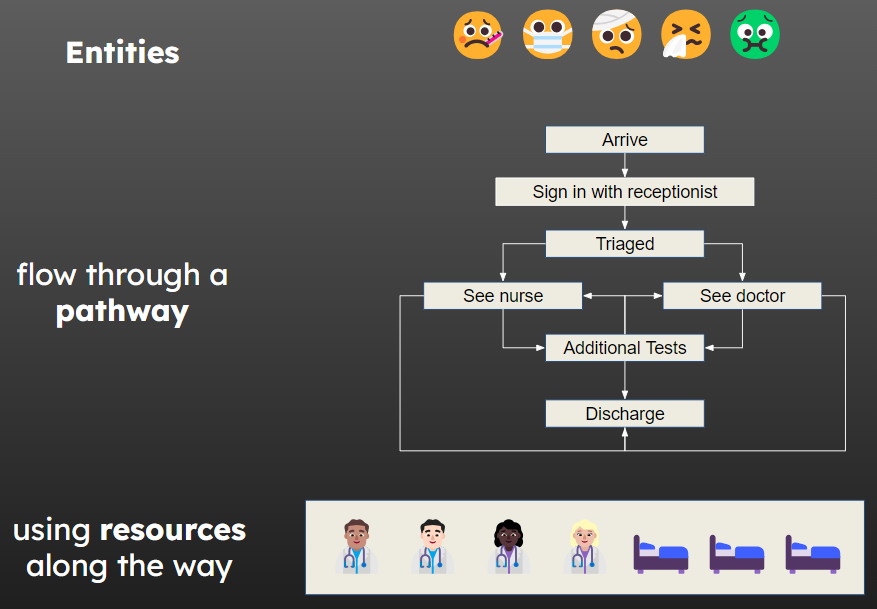
\includegraphics{images/example.png}

In healthcare, DES models can be used to model :

\begin{itemize}
\tightlist
\item
  Patient pathways
\item
  Phone systems
\item
  The transit of test results And more!
\end{itemize}

DES models are extremely useful for asking what if? questions about
process / pathway changes.

\section{Why use DES?}\label{why-use-des}

Discrete event simulation allows you to

\begin{itemize}
\tightlist
\item
  Test changes in a risk-free, low-cost way
\item
  Explore the impact of changes in demand
\item
  See whether a system can cope on bad days as well as good days
\item
  Predict how long it will take to clear an existing backlog
\end{itemize}

This can allow you to optimize a system, leading to better balance and
better flow, which can in turn lead to

\begin{itemize}
\tightlist
\item
  A safer environment
\item
  Less stress for staff
\item
  Improved patient experience
\item
  Meeting targets
\end{itemize}

\section{An example}\label{an-example}

Imagine being able to create a model of an emergency department.

In this model, you can change all sorts of things

\begin{itemize}
\tightlist
\item
  how many doctors, nurses and receptionists there are at each step
\item
  how long it takes for people to be seen
\item
  how many people go into the trauma pathway versus the non-trauma
  pathway
\end{itemize}

Then sprinkle in a dose of randomness - because in real life, you're not
going to have each appointment taking the exact same amount of time, or
people arriving exactly every five minutes - and then you can start to
explore just how well a system will perform, what changes might have the
most impact, and what configuration is likely to perform best. Then you
can run it 1000 times with slightly different random days to see how
well it performs on both good days and bad.

You can polish it all off by visualising the individual entities moving
through the system so people with little understanding of discrete event
simulation can get a sense of what's going on, and you can give them
access to all of the controls - the number of nurses and doctors, the
average consultation length, and more - so that they can explore the
impact of theser changes themselves.

\url{https://github.com/hsma-programme/Teaching_DES_Concepts_Streamlit/assets/29951987/1adc36a0-7bc0-4808-8d71-2d253a855b31}

\section{Runs and Trials}\label{runs-and-trials}

In a stochastic model, it is important that we do not just run a model
once if we're looking to draw insights from our results. This is because
every run of the simulation will have different random samples for
inter-arrival times, activity times etc.

What if you had a run with unusually long activity times sampled (a run
of ``bad luck'')? Or unusually long inter-arrival times (a run of ``good
luck'')?

We need to run a stochastic simulation many times and take summary
statistics over the results from each run to get more representative
results from the model.

A single run of a model for a simulated period of time is known as a
\textbf{run}. A batch of multiple runs with the same parameter values is
known as a \textbf{trial}.

\section{Key DES Terminology}\label{key-des-terminology}

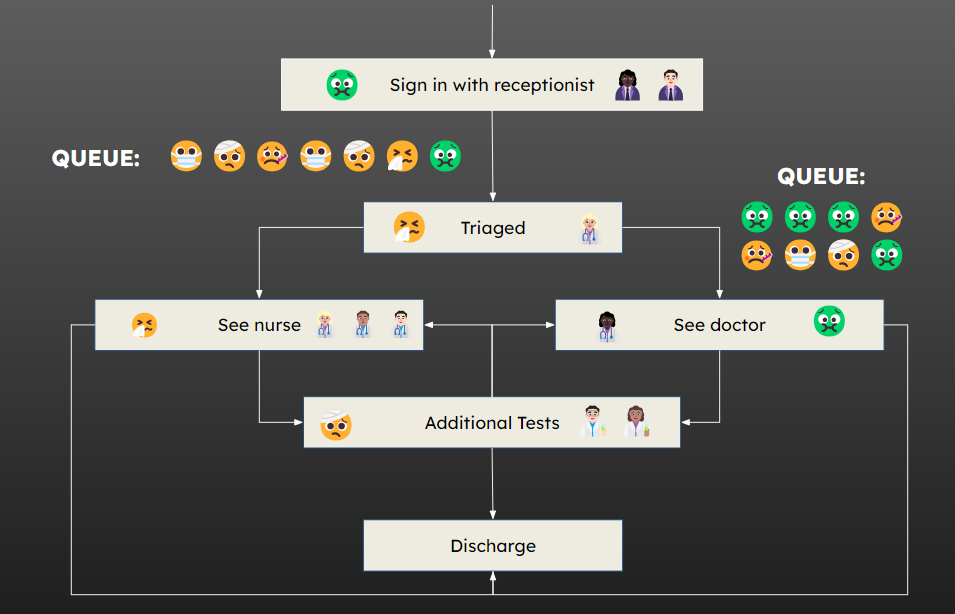
\includegraphics{images/example_des_simple.png}

\textbf{Entities} are the things that are flowing through the sequential
processes in the model (eg patients, test results, callers on a phone)

\textbf{Generators} are the way in which entities enter the model and
come into being (eg arriving at ED by ambulance, self-presenting,
referral from GP)

\textbf{Inter-Arrival Times} specify the time between entities being
generated in the generators (ie the time between arrivals into the
modelled system)

\textbf{Activities} (sometimes referred to as Servers) are the bits of
process that the entities are queuing up for (eg triaged, seen at
reception, speak to doctor etc)

\textbf{Activity Time} represents the amount of time it takes for an
activity to happen to an entity - this is normally stochastic (random)
and drawn from a distribution for each entity (eg time spent with nurse,
time to be treated etc)

\textbf{Resources} are the ``stuff'' and / or ``staff'' required for an
activity to happen to an entity (eg nurse to triage, bed for patient,
consultation room for GP to see patient etc, X-Ray machine and
Radiographer to be free for X-Ray etc). Important - resources may be
shared between activities (eg the same nurse may be required to run
multiple activities in our model, or even things we haven't explicitly
modelled)

\textbf{Queues} hold entities that are waiting for an activity. Entities
wait in a queue until the activity has both the capacity and all
required resources.

\textbf{Sinks} are how entities leave the model (the bit of system we're
modelling)

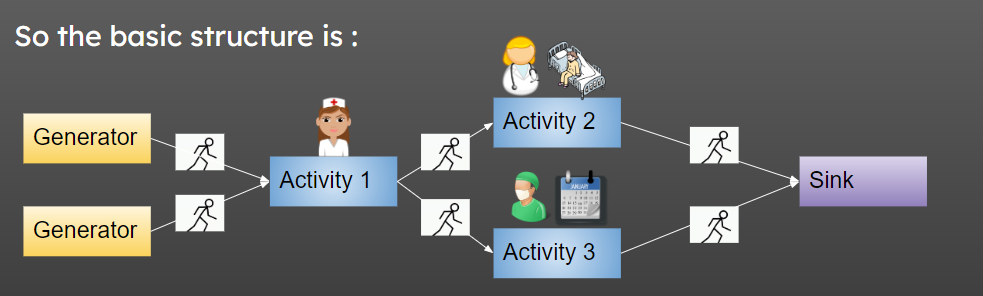
\includegraphics{images/des_steps.png}

\subsection{Entities}\label{entities}

Each entity may have certain ``attributes'' that it ``carries with
them'' to help determine its journey through the modelled system. For
example :

\begin{itemize}
\tightlist
\item
  whether it goes down path A or B
\item
  how long it spends in an activity
\item
  its priority in a queue for an activity
\end{itemize}

There may also be more than one type of entity in a model at the same
time. For example, patients in a clinic, their test results, and phone
calls into the clinic are all entities that we may want to capture when
modelling the clinic.

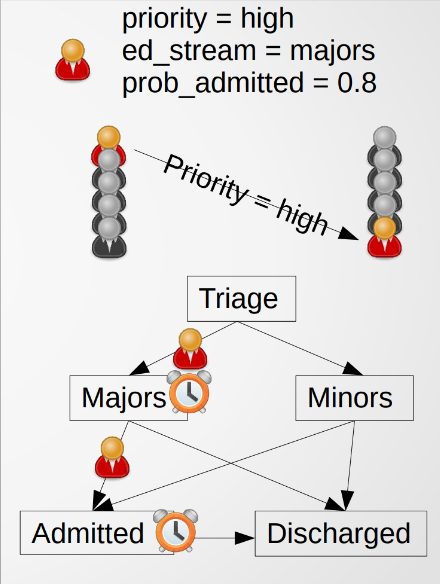
\includegraphics{images/des_entities.png}

\subsection{Generators and
Inter-Arrival}\label{generators-and-inter-arrival}

A generator creates new entities to bring into the system. The rate at
which new entities are generated is determined by an inter-arrival time.

The inter-arrival time determines the time between one entity being
generated, and the next one being generated.

Inter-arrival times may be fixed, but are typically sampled (drawn)
stochastically (randomly) from a distribution to capture variability
(even if the variability is small).

An Exponential Distribution is often used to sample inter-arrival times.
More than one distribution may be used for the same generator (e.g.~for
different times of the day, day of week etc). You may also (often) have
more than one generator in a system.

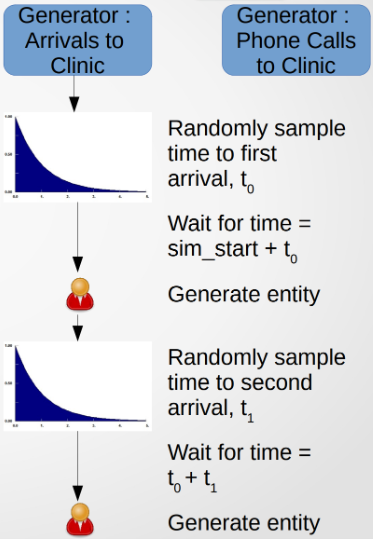
\includegraphics{images/generators_iat.png}

\subsection{Queues}\label{queues}

Each activity in a Discrete Event Simulation has an associated queue.
The queue holds entities whilst they wait for the activity to become
available for them.

Each queue has a queuing policy. This determines the order in which
entities are released from the queue into the activity. The two most
common queuing policies are:

\begin{itemize}
\tightlist
\item
  First In First Out (FIFO) : entities are seen in the order they
  arrive. This is the default.
\item
  Priority-based : entities are seen according to some priority
  attribute. Ties often resolved using FIFO
\end{itemize}

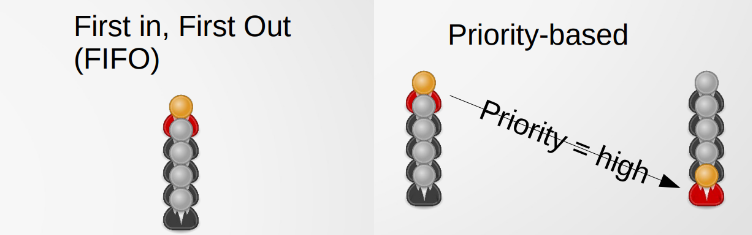
\includegraphics{images/queue_types.png}

\subsection{Activities and Activity
Times}\label{activities-and-activity-times}

Each activity in a DES describes a process -- this may be a simple
atomic task, or a set of tasks bundled together. For an activity to take
place, it needs :

\begin{itemize}
\tightlist
\item
  An entity (drawn from the queue)
\item
  The required type and number of resource to be available
\end{itemize}

Once the above conditions have been met, the activity begins. The
entity, and the resource(s) are then locked in place for an amount of
time -- the Activity Time. The resource(s) cannot be used elsewhere
until the activity time has passed.

Activity times may be fixed, but are typically sampled stochastically
from a distribution.

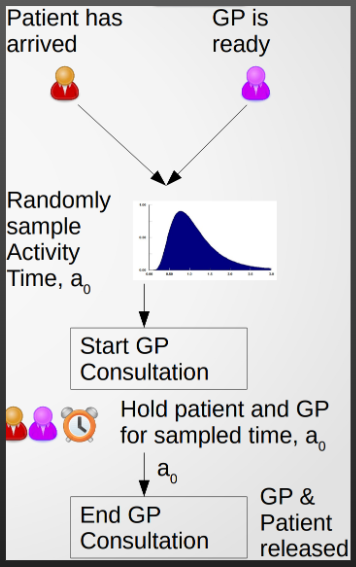
\includegraphics{images/activity_activity_times.png}

\begin{tcolorbox}[enhanced jigsaw, colframe=quarto-callout-tip-color-frame, bottomtitle=1mm, breakable, rightrule=.15mm, coltitle=black, colbacktitle=quarto-callout-tip-color!10!white, opacityback=0, leftrule=.75mm, arc=.35mm, toptitle=1mm, title=\textcolor{quarto-callout-tip-color}{\faLightbulb}\hspace{0.5em}{Tip}, titlerule=0mm, colback=white, toprule=.15mm, bottomrule=.15mm, left=2mm, opacitybacktitle=0.6]

The common distribution for process times is the Log Normal
distributions. However, Exponential Distributions can be a good starting
point, as it's easy to change the ``mean'' when playing around with
things. You can then change to something like a Log Normal once you (and
the stakeholders) are happy

\end{tcolorbox}

\subsection{Resources}\label{resources}

Resources are needed to undertake activities. An activity may require
just a single resource, more than one resource of the same type, or
multiple resources of different types.

\begin{tcolorbox}[enhanced jigsaw, colframe=quarto-callout-tip-color-frame, bottomtitle=1mm, breakable, rightrule=.15mm, coltitle=black, colbacktitle=quarto-callout-tip-color!10!white, opacityback=0, leftrule=.75mm, arc=.35mm, toptitle=1mm, title=\textcolor{quarto-callout-tip-color}{\faLightbulb}\hspace{0.5em}{Tip}, titlerule=0mm, colback=white, toprule=.15mm, bottomrule=.15mm, left=2mm, opacitybacktitle=0.6]

An activity may not require a resource at all, but think carefully to
ensure that it really is either ``resourceless'' or there is no
constraint on the resource (and so doesn't need to be modelled).

Resources can include - ``staff'' (e.g.~doctors, nurses, officers etc) -
``stuff'' (beds, test equipment, detention cell etc)

\end{tcolorbox}

Resources can (and often are) shared across a system, so may be required
for more than one activity. Therefore, a resource drain in one part of
the system can affect another.

All required resources are needed for an activity to take place.

In some activities, having optional additional resource may speed up the
activity (though rarely linearly).

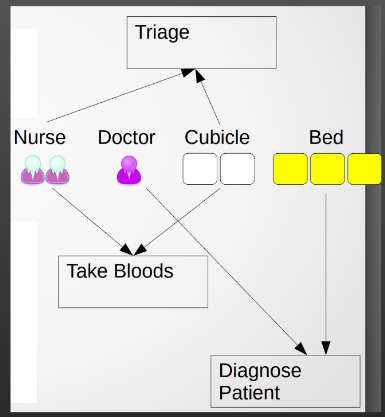
\includegraphics{images/resources_simple.png}

\subsection{Sinks}\label{sinks}

Sinks are how entities leave the system, or part of the system, being
modelled. Sinks might include :

\begin{itemize}
\tightlist
\item
  an entity physically leaving a system (e.g.~discharge from hospital)
\item
  an entity no longer existing (e.g.~death, use of sample, end of
  telephone call)
\item
  an entity no longer needing to access activities that we're interested
  in (e.g.~they leave the bit of the system that we're modelling)
\end{itemize}

The most important thing to remember about a sink is that it doesn't
necessarily represent an entity leaving the system entirely.

For example, the scope of your model may only cover the triage aspect of
an Emergency Department. Therefore, a valid sink might be placed after
their triage - they've left the scope of our model

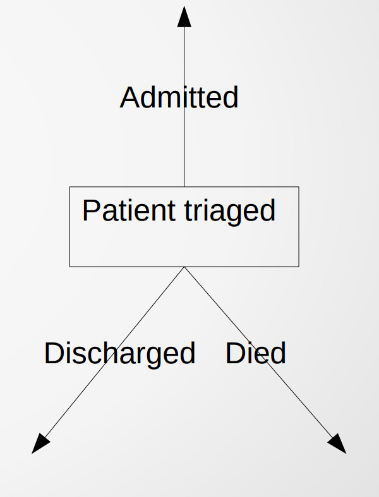
\includegraphics{images/sinks_simple.png}

\subsection{Branching Paths}\label{branching-paths}

Real world systems (and the models of those systems) are rarely linear.
Often, different things will happen to different entities. In a Discrete
Event Simulation, this means different entities flowing to different
activities, or different sinks.

We might differentiate based on :

\begin{itemize}
\tightlist
\item
  an attribute of the patient (e.g.~patients with a higher priority
  value flow through a different set of activities)
\item
  probability (e.g.~we know that approx 60\% of these patients end up
  being admitted, so we'll randomly select for them to be admitted 60\%
  of the time)
\item
  time (e.g.~after a certain time of day, entities flow through a
  different set of activities)
\end{itemize}

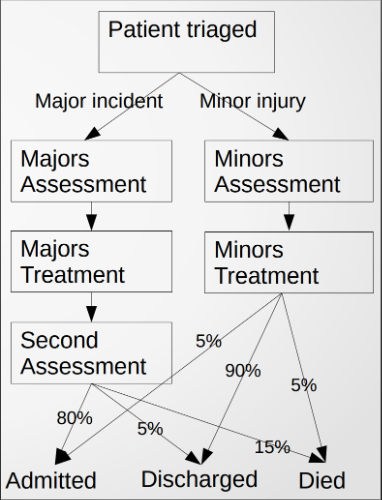
\includegraphics{images/branching_paths_simple.png}

\subsection{Outputs}\label{outputs}

As with any type of model, it's important to think about what outputs
you need your DES model to generate to answer your modelling questions.
As a DES model is used to model queuing and resourcing problems, typical
DES model outputs include average, min, max, xth percentile of :

\begin{itemize}
\tightlist
\item
  time entities are in system
\item
  queue length and duration for queues of interest
\item
  rate of resource utilisation (ie \% of time a resource is in use for
  activities in the model)
\item
  probability of exceeding a defined queue length / queue time /
  resource utilisation threshold (e.g.~4 hour wait in ED, overcrowding
  thresholds)
\end{itemize}

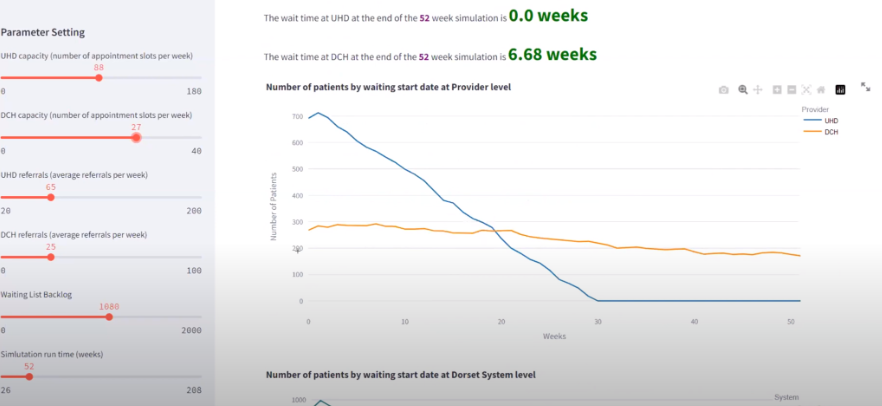
\includegraphics{images/output_example_simple.png}

\chapter{Exercise - Designing a DES}\label{exercise---designing-a-des}

Design a Discrete Event Simulation for a system of your choosing.

Think about some different possibilities (and these don't have to be
health-related, they can be anything! A restaurant? Airport? Customer
service line?).

You should then draw up a design for the model. This should include :

\begin{itemize}
\tightlist
\item
  The ``what if?'' question(s) you would use the model to answer
\item
  A process map of the system you are looking to model
\item
  A conceptual model for the proposed Discrete Event Simulation (which
  may not include everything in the process map).
\end{itemize}

Identify the types of entities, generators, activities, queues,
resources and sinks.

Describe what each of your inter-arrival times and activity times
represent, and from where you might draw the data.

Consider the scope, level of detail etc when designing your model. What
do you need to model to answer your question? How can you simplify your
model?

\begin{tcolorbox}[enhanced jigsaw, colframe=quarto-callout-tip-color-frame, bottomtitle=1mm, breakable, rightrule=.15mm, coltitle=black, colbacktitle=quarto-callout-tip-color!10!white, opacityback=0, leftrule=.75mm, arc=.35mm, toptitle=1mm, title=\textcolor{quarto-callout-tip-color}{\faLightbulb}\hspace{0.5em}{Tip}, titlerule=0mm, colback=white, toprule=.15mm, bottomrule=.15mm, left=2mm, opacitybacktitle=0.6]

The website \href{https://app.diagrams.net/}{draw.io (also known as
diagrams.net)} is a great free resource for creating process maps.

\end{tcolorbox}

\part{Part 2 - Your First SimPy Model}

\chapter{An Introduction to SimPy}\label{an-introduction-to-simpy}

SimPy is a Python package that allows us to create powerful Discrete
Event Simulation (DES) models.

You can read SimPy's own tutorials and reference guides on its website :
https://simpy.readthedocs.io/en/latest/ - but we'd recommend working
through at least the first few chapters in this book first.

To install SimPy, we need to \texttt{pip\ install\ simpy}. However, it
is recommended that you use a separate environment. Make sure you switch
to this environment for any DES work you do - or, even better, set up a
separate environment for every DES project you undertake!

Before we look at how we put together a SimPy model, there's a couple
concepts we need to cover first that are important to understand.

\section{Simulation Time}\label{simulation-time}

SimPy simulations run in time units. These units of time can represent
any real world amount of time we like as long as we are consistent
within the same model.

Our time units should represent the lowest level of real world time that
we need to represent in the model. In models of pathways where people
arrive for a service, this will likely be minutes (seconds is too much,
and hours is probably not enough, unless all the processes are slow).
But we may have pathways where we measure time in days or weeks
(e.g.~referral pathways).

For example, in an ED model, our time units may represent minutes. So we
specify everything in minutes - inter-arrival times, activity times etc.

Strictly speaking, SimPy doesn't run in time units ticking away one by
one. Instead, it schedules events jumps to the next event. But don't
worry about that for your purposes. Just know that, because of this, you
will see current simulation time as floating point numbers (eg the
current time unit could be 3.6 etc).

\section{Generator Functions}\label{generator-functions}

SimPy is built around a special type of function in Python known as a
Generator Function.

So let's have a look at what we mean by a Generator Function.

Conventional functions in Python are called, then run with some
(optional) inputs, and then finish (usually by returning some output).
When we call the function again, it runs again, from scratch.

Generator functions remember where they were and what they did when
control is passed back (they retain their local state), so that they can
continue where they left off, and can be used as powerful iterators (for
and while loops are other examples of iterators).

This is very useful where we want state to be maintained, so we can
remember how long until we generate the next entity, or where an entity
is in a pathway\ldots{}

Let's look at a very simple example of a generator function to see how
they work.

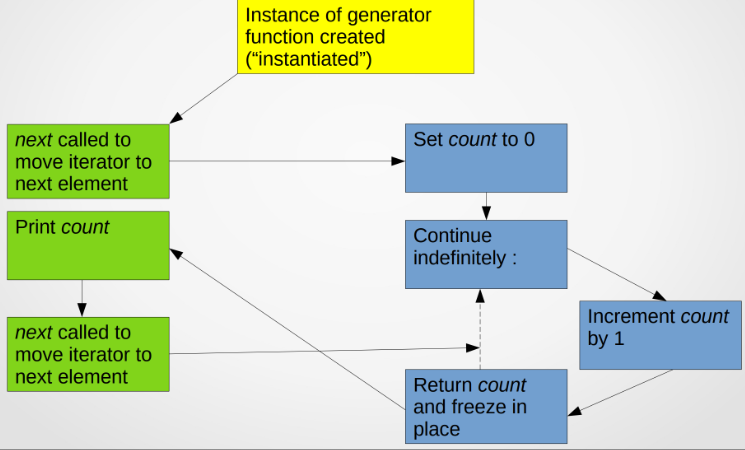
\includegraphics{images/generator_func_example.png}

In SimPy, we use Generator Functions in two different places :

To model the DES generators (arrival points) To model the individual
journey of each entity

Let's imagine we are modelling patients in a patient pathway.

For 1, the generator function basically creates a patient, sets them off
on their pathway, then freezes in place for an amount of time
representing the inter-arrival time to the next patient. Then it does it
all over again.

For 2, the generator function requests a resource and freezes until that
resource is available (the queue). When the resource is available it
freezes in place for an amount of time with it (the activity). It will
then either move on to the next activity (and request the resource for
it, as above) or end if there are no further activities.

\chapter{The Recommended Structure for DES
Models}\label{the-recommended-structure-for-des-models}

There are many different ways to structure SimPy models.

You will often find different coders have their own preferred approach!

We're going to structure our SimPy model in an Object Oriented way.

\begin{tcolorbox}[enhanced jigsaw, colframe=quarto-callout-note-color-frame, bottomtitle=1mm, breakable, rightrule=.15mm, coltitle=black, colbacktitle=quarto-callout-note-color!10!white, opacityback=0, leftrule=.75mm, arc=.35mm, toptitle=1mm, title=\textcolor{quarto-callout-note-color}{\faInfo}\hspace{0.5em}{Note}, titlerule=0mm, colback=white, toprule=.15mm, bottomrule=.15mm, left=2mm, opacitybacktitle=0.6]

There are two main ways of programming in python - \textbf{functional}
and \textbf{object oriented}. These are known as coding
\textbf{paradigms}.

In functional programming, you write \textbf{functions} that are
(ideally) designed to do one thing and do it well.

You then use these functions in some sort of sequence to achieve what
you're trying to do.

This can make a lot of sense for a lot of data analysis and data science
workflows.

In comparison, in object oriented programming (OOP) everything is
centred around objects that have their own

\begin{itemize}
\tightlist
\item
  attributes (variables that belong to them) and
\item
  methods (which are what functions are called when they belong to
  objects).
\end{itemize}

\textbf{Objects} are created as \textbf{instances} of \textbf{classes}.

Classes are essentially generalised blueprints for how certain types of
objects should work!

This can be really useful in situations where you have either

\begin{itemize}
\tightlist
\item
  a lot of logic that makes sense to attach and organise with the thing
  that uses that logic (like a process)
\item
  a need to make copies of a very similar thing (like lots of patients
  to populate a model)
\end{itemize}

Let's look at an example.

Let's say we want to write code that defines how an ambulance works.

There will be properties the ambulance has. Things like :

\begin{itemize}
\tightlist
\item
  The organisation it belongs to
\item
  The registration number
\item
  Whether a patient is currently on board
\item
  Whether the siren is currently going off
\end{itemize}

There will also be things the ambulance does :

\begin{itemize}
\tightlist
\item
  Driving
\item
  Parking
\item
  Having patients loaded into it / out of it
\item
  Switching the siren on and off
\end{itemize}

In Object Oriented Programming, the things it \textbf{has} are known as
\textbf{attributes} and the things it \emph{does} are \emph{methods}.

\end{tcolorbox}

Specifically, we're going to have 4 different classes: g, entity, model,
and trial.

While object oriented code can feel a bit cumbersome for small models,
following the same sort of pattern each time makes it really easy to
keep track of what your model is doing. It also makes it a lot easier to
expand and modify your model over time.

The other benefit is that you will find other models from people who
have done the HSMA course are likely to have a similar structure - so
you should find it easier to read, reuse and tweak their models too!

\begin{tcolorbox}[enhanced jigsaw, colframe=quarto-callout-note-color-frame, bottomtitle=1mm, breakable, rightrule=.15mm, coltitle=black, colbacktitle=quarto-callout-note-color!10!white, opacityback=0, leftrule=.75mm, arc=.35mm, toptitle=1mm, title=\textcolor{quarto-callout-note-color}{\faInfo}\hspace{0.5em}{Note}, titlerule=0mm, colback=white, toprule=.15mm, bottomrule=.15mm, left=2mm, opacitybacktitle=0.6]

Even among people using an object oriented approach, you will find some
variations.

Again, there's nothing wrong with that!

Another common pattern you may come across in time is the Scenario,
entity, model approach with single\_run and multiple\_run functions that
don't exist inside a class.

Over time, you'll likely find a style used by someone else that you find
particularly easy to follow and you want to adopt and adapt.

\end{tcolorbox}

\textbf{g Class}

This is a special class that will store our global level parameters for
the model.

Unlike most OOP cases, we won't create an instance of this class (hence
the lower case) - we'll just refer to the blueprint directly.

\textbf{Entity}

This class will represent our entity.

An entity could be a customer, a passenger, etc., but often in our
healthcare models, our entities will be patients.

Entities will carry with them information that we can record to and / or
read from (e.g.~an ID, how long they spent queuing, their condition
etc).

If we had more than one entity, we'd need a class for each.

Multiple entities could be different types of patients - e.g.~trauma
patients and non-trauma patients.

\textbf{Model}

This is the big one that represents the system that we are modelling.

This could be a phone helpline, a clinic, an emergency department, an
airport terminal, a healthcare clinic that runs appointments - many
processes are suitable.

It'll have our generators, our entity journeys and more, and it's where
our SimPy environment (where everything lives) will be kept.

\textbf{Trial}

This class will represent a batch of runs of our simulation, and will
have methods to run a trial, extract results etc.

\section{Class breakdown}\label{class-breakdown}

Let's look at the purpose and recommended structure of each class in a
bit more detail.

Here, the example code given relates to a customer support helpline.
Customers call a helpline, wait on hold until a customer support agent
is ready to speak to them, speak to the agent for a period of time, and
then the call ends and the agent connects to the next person who is
waiting on hold. If there is no-one on hold at the time, the agent will
get a break until someone else arrives!

\subsection{g Class}\label{g-class}

The g Class stores our global parameter values for the model so we can
easily change aspects of the model to test scenarios. This includes :

\begin{itemize}
\tightlist
\item
  Values to define inter-arrival time distributions (eg mean, standard
  deviation etc)
\item
  Values to define activity time distributions (eg mean, standard
  deviation etc)
\item
  Number of each resource
\item
  Duration of simulation runs
\item
  Number of runs in a trial
\end{itemize}

We do not create an instance of g class. Instead, we refer to it
directly when we need to access something in it.

\begin{tcolorbox}[enhanced jigsaw, colframe=quarto-callout-note-color-frame, bottomtitle=1mm, breakable, rightrule=.15mm, coltitle=black, colbacktitle=quarto-callout-note-color!10!white, opacityback=0, leftrule=.75mm, arc=.35mm, toptitle=1mm, title=\textcolor{quarto-callout-note-color}{\faInfo}\hspace{0.5em}{Example g class}, titlerule=0mm, colback=white, toprule=.15mm, bottomrule=.15mm, left=2mm, opacitybacktitle=0.6]

\begin{Shaded}
\begin{Highlighting}[]
\KeywordTok{class}\NormalTok{ g:}
\NormalTok{    time\_units\_between\_customer\_arrivals }\OperatorTok{=} \DecValTok{5}
\NormalTok{    mean\_customer\_service\_time }\OperatorTok{=} \DecValTok{6}
\NormalTok{    number\_of\_customer\_support\_agents }\OperatorTok{=} \DecValTok{1}
\NormalTok{    sim\_duration }\OperatorTok{=} \DecValTok{1440}
\NormalTok{    number\_of\_runs }\OperatorTok{=} \DecValTok{10}
\end{Highlighting}
\end{Shaded}

\end{tcolorbox}

\subsection{Entity class}\label{entity-class}

The entity class represents our entity in the model - which, for
healthcare models, will often be patients.

We can store attributes here that entities carry with them that we may
want to access (think of a person carrying a clipboard with them with
information on it).

In a simple model, an entity may just carry their ID and how long they
spent queuing for a resource (once known). But more advanced models
could store things like their condition, their priority, probability of
going down path x, etc.

\begin{tcolorbox}[enhanced jigsaw, colframe=quarto-callout-note-color-frame, bottomtitle=1mm, breakable, rightrule=.15mm, coltitle=black, colbacktitle=quarto-callout-note-color!10!white, opacityback=0, leftrule=.75mm, arc=.35mm, toptitle=1mm, title=\textcolor{quarto-callout-note-color}{\faInfo}\hspace{0.5em}{Example entity class}, titlerule=0mm, colback=white, toprule=.15mm, bottomrule=.15mm, left=2mm, opacitybacktitle=0.6]

\begin{Shaded}
\begin{Highlighting}[]
\KeywordTok{class}\NormalTok{ Customer:}
    \KeywordTok{def} \FunctionTok{\_\_init\_\_}\NormalTok{(}\VariableTok{self}\NormalTok{, p\_id):}
        \VariableTok{self}\NormalTok{.}\BuiltInTok{id} \OperatorTok{=}\NormalTok{ p\_id}
        \VariableTok{self}\NormalTok{.queue\_time\_customer\_support\_agent }\OperatorTok{=} \DecValTok{0}
\end{Highlighting}
\end{Shaded}

\end{tcolorbox}

\subsection{Model Class}\label{model-class}

The Model Class represents the system we are modelling - this might be a
clinic, for example. As such, there's a lot more to unpack here, so
let's take this bit by bit.

First, we'll look at the constructor for our model.

The constructor will set up - a SimPy Environment (basically where
everything lives) - an entity counter (which we'll use to give entities
- such as patients - a simple ID) - the resources we need (for example,
our nurses) - a DataFrame to store per-entity results in a single run of
the model - attributes to store things like how long the entities queued
for each activity

What the constructor sets up doesn't have to be limited to these things
- anything relating to the system as a whole that makes sense to store
here could be included.

\subsubsection{DES generator - arrivals of entities to the
system}\label{des-generator---arrivals-of-entities-to-the-system}

Within the Model Class we have a \textbf{generator function} that will
represent our DES generator for entities \textbf{arriving into our
process}.

Here's basically how it works:

\emph{KEEP REPEATING THE FOLLOWING FOREVER (until the simulation stops
running) :}

\begin{enumerate}
\def\labelenumi{\arabic{enumi}.}
\tightlist
\item
  Increment the counter to get ID for next entity
\item
  Create a new entity and give them that ID
\item
  Start up an instance of the generator function for their journey
  through the process and chuck them in it
\item
  Sample the time until the next entity arrives
\item
  FREEZE this function until that time elapses
\item
  Return to 1
\end{enumerate}

\subsubsection{DES Generator - the entity
journey}\label{des-generator---the-entity-journey}

Now, let's look at the big one. The other generator function - the one
that represents an entity's journey through the system (this is the one
we lobbed the new entities generated by the previous generator).

Here's how this works :

\begin{enumerate}
\def\labelenumi{\arabic{enumi}.}
\tightlist
\item
  Record time started queuing for first activity
\item
  Request resource for first activity
\item
  Wait until resource is free
\item
  Once resource is free, grab the resource and keep hold of the resource
  until finished with them. Record time finished queuing and calculate
  queue time.
\item
  Sample how long will spend in this activity.
\item
  FREEZE this instance of the function until that time elapses (freezing
  the resource with it, so it's not available to anyone else)
\item
  If there's another activity, do the same again for that one. If not,
  end (and therefore entity leaves the model).
\end{enumerate}

\subsubsection{Running the model}\label{running-the-model}

Finally, we need a run method in our Model class. Basically, the run
method will

\begin{itemize}
\tightlist
\item
  start up our DES generators (our arrival points) - we only have one
  here.
\item
  tell the simulation to run for the duration specified in g Class.
\item
  call the calculate run results method in the previous slide.
\item
  print out the run number with the patient-level results from this run.
\end{itemize}

\begin{tcolorbox}[enhanced jigsaw, colframe=quarto-callout-note-color-frame, bottomtitle=1mm, breakable, rightrule=.15mm, coltitle=black, colbacktitle=quarto-callout-note-color!10!white, opacityback=0, leftrule=.75mm, arc=.35mm, toptitle=1mm, title=\textcolor{quarto-callout-note-color}{\faInfo}\hspace{0.5em}{Full Example model class}, titlerule=0mm, colback=white, toprule=.15mm, bottomrule=.15mm, left=2mm, opacitybacktitle=0.6]

\begin{Shaded}
\begin{Highlighting}[]
\KeywordTok{class}\NormalTok{ Model:}
    \CommentTok{\# Constructor to set up the model for a run.  We pass in a run number when}
    \CommentTok{\# we create a new model.}
    \KeywordTok{def} \FunctionTok{\_\_init\_\_}\NormalTok{(}\VariableTok{self}\NormalTok{, run\_number):}
        \CommentTok{\# Create a SimPy environment in which everything will live}
        \VariableTok{self}\NormalTok{.env }\OperatorTok{=}\NormalTok{ simpy.Environment()}

        \CommentTok{\# Create a customer counter (which we\textquotesingle{}ll use as a customer ID)}
        \VariableTok{self}\NormalTok{.customer\_counter }\OperatorTok{=} \DecValTok{0}

        \CommentTok{\# Create a SimPy resource to represent a customer support agent, that will live in the}
        \CommentTok{\# environment created above.  The number of this resource we have is}
        \CommentTok{\# specified by the capacity, and we grab this value from our g class.}
        \VariableTok{self}\NormalTok{.customer\_support\_agent }\OperatorTok{=}\NormalTok{ simpy.Resource(}\VariableTok{self}\NormalTok{.env, capacity}\OperatorTok{=}\NormalTok{number\_of\_customer\_support\_agents)}

        \CommentTok{\# Store the passed in run number}
        \VariableTok{self}\NormalTok{.run\_number }\OperatorTok{=}\NormalTok{ run\_number}

        \CommentTok{\# Create a new Pandas DataFrame that will store some results against}
        \CommentTok{\# the customer ID (which we\textquotesingle{}ll use as the index).}
        \VariableTok{self}\NormalTok{.results\_df }\OperatorTok{=}\NormalTok{ pd.DataFrame()}
        \VariableTok{self}\NormalTok{.results\_df[}\StringTok{"Customer ID"}\NormalTok{] }\OperatorTok{=}\NormalTok{ [}\DecValTok{1}\NormalTok{]}
        \VariableTok{self}\NormalTok{.results\_df[}\StringTok{"Queue Time"}\NormalTok{] }\OperatorTok{=}\NormalTok{ [}\FloatTok{0.0}\NormalTok{]}
        \VariableTok{self}\NormalTok{.results\_df[}\StringTok{"Time with Customer Support Agent"}\NormalTok{] }\OperatorTok{=}\NormalTok{ [}\FloatTok{0.0}\NormalTok{]}
        \VariableTok{self}\NormalTok{.results\_df.set\_index(}\StringTok{"Customer ID"}\NormalTok{, inplace}\OperatorTok{=}\VariableTok{True}\NormalTok{)}

        \CommentTok{\# Create an attribute to store the mean queuing time for the support agents}
        \CommentTok{\# across this run of the model}
        \VariableTok{self}\NormalTok{.mean\_queue\_time\_support\_agent }\OperatorTok{=} \DecValTok{0}

    \CommentTok{\# A generator function that represents the DES generator for customer}
    \CommentTok{\# arrivals}
    \KeywordTok{def}\NormalTok{ generator\_customer\_arrivals(}\VariableTok{self}\NormalTok{):}
        \CommentTok{\# We use an infinite loop here to keep doing this indefinitely whilst}
        \CommentTok{\# the simulation runs}
        \ControlFlowTok{while} \VariableTok{True}\NormalTok{:}
            \CommentTok{\# Increment the customer counter by 1 (this means our first customer}
            \CommentTok{\# will have an ID of 1)}
            \VariableTok{self}\NormalTok{.customer\_counter }\OperatorTok{+=} \DecValTok{1}

            \CommentTok{\# Create a new customer {-} an instance of the customer Class we}
            \CommentTok{\# defined above.  Remember, we pass in the ID when creating a}
            \CommentTok{\# customer {-} so here we pass the customer counter to use as the ID.}
\NormalTok{            c }\OperatorTok{=}\NormalTok{ Customer(}\VariableTok{self}\NormalTok{.customer\_counter)}

            \CommentTok{\# Tell SimPy to start up the use\_customer\_service\_helpline generator function with}
            \CommentTok{\# this customer (the generator function that will model the}
            \CommentTok{\# customer\textquotesingle{}s journey through the system)}
            \VariableTok{self}\NormalTok{.env.process(}\VariableTok{self}\NormalTok{.use\_customer\_service\_helpline (c))}

            \CommentTok{\# Randomly sample the time to the next customer arriving.  Here, we}
            \CommentTok{\# sample from an exponential distribution (common for inter{-}arrival}
            \CommentTok{\# times), and pass in a lambda value of 1 / mean.  The mean}
            \CommentTok{\# inter{-}arrival time is stored in the g class.}
\NormalTok{            sampled\_inter\_arrival\_time }\OperatorTok{=}\NormalTok{ random.expovariate(}\FloatTok{1.0} \OperatorTok{/}\NormalTok{ g.time\_units\_between\_customer\_arrivals)}

            \CommentTok{\# Freeze this instance of this function in place until the}
            \CommentTok{\# inter{-}arrival time we sampled above has elapsed.  Note {-} time in}
            \CommentTok{\# SimPy progresses in "Time Units", which can represent anything}
            \CommentTok{\# you like (just make sure you\textquotesingle{}re consistent within the model)}
            \ControlFlowTok{yield} \VariableTok{self}\NormalTok{.env.timeout(sampled\_inter\_arrival\_time)}

    \CommentTok{\# A generator function that represents the pathway for a customer calling our helpline}
    \CommentTok{\# Here the pathway is extremely simple {-} a customer}
    \CommentTok{\# arrives in the call system, waits to be connected to a customer support agent,}
    \CommentTok{\# spends a varying amount of time being helped by the agent, and then leaves,}
    \CommentTok{\# meaning the agent is free to help the next person.}
    \CommentTok{\# The customer object is passed in to the generator function so we can}
    \CommentTok{\# extract information from / record information to it}
    \KeywordTok{def}\NormalTok{ use\_customer\_service\_helpline(}\VariableTok{self}\NormalTok{, customer):}
        \CommentTok{\# Record the time the patient started queuing for a nurse}
\NormalTok{        start\_q\_customer\_support\_agent }\OperatorTok{=} \VariableTok{self}\NormalTok{.env.now}

        \CommentTok{\# This code says request a customer support agent resource, and do all of the following}
        \CommentTok{\# block of code with that nurse resource held in place (and therefore}
        \CommentTok{\# not usable by another patient)}
        \ControlFlowTok{with} \VariableTok{self}\NormalTok{.customer\_support\_agent.request() }\ImportTok{as}\NormalTok{ req:}
            \CommentTok{\# Freeze the function until the request for a customer support agent can be met.}
            \CommentTok{\# The customer is currently queuing.}
            \ControlFlowTok{yield}\NormalTok{ req}

            \CommentTok{\# When we get to this bit of code, control has been passed back to}
            \CommentTok{\# the generator function, and therefore the request for a customer support agent has}
            \CommentTok{\# been met.  We now have the customer support agent, and have stopped queuing, so we}
            \CommentTok{\# can record the current time as the time we finished queuing.}
\NormalTok{            end\_q\_customer\_support\_agent }\OperatorTok{=} \VariableTok{self}\NormalTok{.env.now}

            \CommentTok{\# Calculate the time this patient was queuing for the customer support agent, and}
            \CommentTok{\# record it in the customer\textquotesingle{}s attribute for this.}
\NormalTok{            customer.queue\_time\_customer\_support\_agent }\OperatorTok{=}\NormalTok{ end\_q\_customer\_support\_agent }\OperatorTok{{-}}\NormalTok{ start\_q\_customer\_support\_agent}

            \CommentTok{\# Now we\textquotesingle{}ll randomly sample the time this customer with the customer support agent.}
            \CommentTok{\# Here, we use an Exponential distribution for simplicity, but you}
            \CommentTok{\# would typically use a Log Normal distribution for a real model}
            \CommentTok{\# (we\textquotesingle{}ll come back to that).  As with sampling the inter{-}arrival}
            \CommentTok{\# times, we grab the mean from the g class, and pass in 1 / mean}
            \CommentTok{\# as the lambda value.}
\NormalTok{            sampled\_customer\_support\_agent\_activity\_time }\OperatorTok{=}\NormalTok{ random.expovariate(}\FloatTok{1.0} \OperatorTok{/}
\NormalTok{                                                        g.mean\_customer\_service\_time)}

            \CommentTok{\# Here we\textquotesingle{}ll store the queuing time for the customer support agent and the sampled}
            \CommentTok{\# time to spend with the nurse in the results DataFrame against the}
            \CommentTok{\# ID for this customer.}
            \CommentTok{\#}
            \CommentTok{\# In real world models, you may not want to}
            \CommentTok{\# bother storing the sampled activity times {-} but as this is a}
            \CommentTok{\# simple model, we\textquotesingle{}ll do it here.}
            \CommentTok{\#}
            \CommentTok{\# We use a handy property of pandas called .at, which works a bit}
            \CommentTok{\# like .loc.  .at allows us to access (and therefore change) a}
            \CommentTok{\# particular cell in our DataFrame by providing the row and column.}
            \CommentTok{\# Here, we specify the row as the patient ID (the index), and the}
            \CommentTok{\# column for the value we want to update for that patient.}
            \VariableTok{self}\NormalTok{.results\_df.at[customer.}\BuiltInTok{id}\NormalTok{, }\StringTok{"Queue Time"}\NormalTok{] }\OperatorTok{=}\NormalTok{ (}
\NormalTok{                customer.queue\_time\_customer\_support\_agent)}
            \VariableTok{self}\NormalTok{.results\_df.at[customer.}\BuiltInTok{id}\NormalTok{, }\StringTok{"Time with Customer Support Agent"}\NormalTok{] }\OperatorTok{=}\NormalTok{ (}
\NormalTok{                sampled\_customer\_support\_agent\_activity\_time)}

            \CommentTok{\# Freeze this function in place for the activity time we sampled}
            \CommentTok{\# above.  This is the patient spending time with the customer support}
            \CommentTok{\# agent.}
            \ControlFlowTok{yield} \VariableTok{self}\NormalTok{.env.timeout(sampled\_customer\_support\_agent\_activity\_time)}

            \CommentTok{\# When the time above elapses, the generator function will return}
            \CommentTok{\# here.  As there\textquotesingle{}s nothing more that we\textquotesingle{}ve written, the function}
            \CommentTok{\# will simply end.  This is a sink.  We could choose to add}
            \CommentTok{\# something here if we wanted to record something {-} e.g. a counter}
            \CommentTok{\# for number of patients that left, recording something about the}
            \CommentTok{\# patients that left at a particular sink etc.}

    \CommentTok{\# This method calculates results over a single run.  Here we just calculate}
    \CommentTok{\# a mean, but in real world models you\textquotesingle{}d probably want to calculate more.}
    \KeywordTok{def}\NormalTok{ calculate\_run\_results(}\VariableTok{self}\NormalTok{):}
        \CommentTok{\# Take the mean of the queuing times for the nurse across patients in}
        \CommentTok{\# this run of the model.}
        \VariableTok{self}\NormalTok{.mean\_queue\_time\_support\_agent }\OperatorTok{=} \VariableTok{self}\NormalTok{.results\_df[}\StringTok{"Time with Customer Support Agent"}\NormalTok{].mean()}

    \CommentTok{\# The run method starts up the DES entity generators, runs the simulation,}
    \CommentTok{\# and in turns calls anything we need to generate results for the run}
    \KeywordTok{def}\NormalTok{ run(}\VariableTok{self}\NormalTok{):}
        \CommentTok{\# Start up our DES entity generators that create new customers.  We\textquotesingle{}ve}
        \CommentTok{\# only got one in this model, but we\textquotesingle{}d need to do this for each one if}
        \CommentTok{\# we had multiple generators.}
        \VariableTok{self}\NormalTok{.env.process(}\VariableTok{self}\NormalTok{.generator\_customer\_arrivals())}

        \CommentTok{\# Run the model for the duration specified in g class}
        \VariableTok{self}\NormalTok{.env.run(until}\OperatorTok{=}\NormalTok{g.sim\_duration)}

        \CommentTok{\# Now the simulation run has finished, call the method that calculates}
        \CommentTok{\# run results}
        \VariableTok{self}\NormalTok{.calculate\_run\_results()}

        \CommentTok{\# Print the run number with the customer{-}level results from this run of}
        \CommentTok{\# the model}
        \BuiltInTok{print}\NormalTok{ (}\SpecialStringTok{f"Run Number }\SpecialCharTok{\{}\VariableTok{self}\SpecialCharTok{.}\NormalTok{run\_number}\SpecialCharTok{\}}\SpecialStringTok{"}\NormalTok{)}
        \BuiltInTok{print}\NormalTok{ (}\VariableTok{self}\NormalTok{.results\_df)}
\end{Highlighting}
\end{Shaded}

\end{tcolorbox}

\subsection{Trial class}\label{trial-class}

Our final class is the Trial class. This represents a batch of
simulation runs, and will contain methods to run a batch of runs, as
well as store, record and display results from the trial.

\begin{tcolorbox}[enhanced jigsaw, colframe=quarto-callout-note-color-frame, bottomtitle=1mm, breakable, rightrule=.15mm, coltitle=black, colbacktitle=quarto-callout-note-color!10!white, opacityback=0, leftrule=.75mm, arc=.35mm, toptitle=1mm, title=\textcolor{quarto-callout-note-color}{\faInfo}\hspace{0.5em}{Example trial class}, titlerule=0mm, colback=white, toprule=.15mm, bottomrule=.15mm, left=2mm, opacitybacktitle=0.6]

\begin{Shaded}
\begin{Highlighting}[]
\KeywordTok{class}\NormalTok{ Trial:}
    \CommentTok{\# The constructor sets up a pandas dataframe that will store the key}
    \CommentTok{\# results from each run (just the mean queuing time for the nurse here)}
    \CommentTok{\# against run number, with run number as the index.}
    \KeywordTok{def}  \FunctionTok{\_\_init\_\_}\NormalTok{(}\VariableTok{self}\NormalTok{):}
        \VariableTok{self}\NormalTok{.df\_trial\_results }\OperatorTok{=}\NormalTok{ pd.DataFrame()}
        \VariableTok{self}\NormalTok{.df\_trial\_results[}\StringTok{"Run Number"}\NormalTok{] }\OperatorTok{=}\NormalTok{ [}\DecValTok{0}\NormalTok{]}
        \VariableTok{self}\NormalTok{.df\_trial\_results[}\StringTok{"Mean Queue Time Customer Supoprt Agent"}\NormalTok{] }\OperatorTok{=}\NormalTok{ [}\FloatTok{0.0}\NormalTok{]}
        \VariableTok{self}\NormalTok{.df\_trial\_results.set\_index(}\StringTok{"Run Number"}\NormalTok{, inplace}\OperatorTok{=}\VariableTok{True}\NormalTok{)}

    \CommentTok{\# Method to print out the results from the trial.  In real world models,}
    \CommentTok{\# you\textquotesingle{}d likely save them as well as (or instead of) printing them}
    \KeywordTok{def}\NormalTok{ print\_trial\_results(}\VariableTok{self}\NormalTok{):}
        \BuiltInTok{print}\NormalTok{ (}\StringTok{"Trial Results"}\NormalTok{)}
        \BuiltInTok{print}\NormalTok{ (}\VariableTok{self}\NormalTok{.df\_trial\_results)}

    \CommentTok{\# Method to run a trial}
    \KeywordTok{def}\NormalTok{ run\_trial(}\VariableTok{self}\NormalTok{):}
        \CommentTok{\# Run the simulation for the number of runs specified in g class.}
        \CommentTok{\# For each run, we create a new instance of the Model class and call its}
        \CommentTok{\# run method, which sets everything else in motion.  Once the run has}
        \CommentTok{\# completed, we grab out the stored run results (just mean queuing time}
        \CommentTok{\# here) and store it against the run number in the trial results}
        \CommentTok{\# dataframe.}
        \ControlFlowTok{for}\NormalTok{ run }\KeywordTok{in} \BuiltInTok{range}\NormalTok{(g.number\_of\_runs):}
\NormalTok{            my\_model }\OperatorTok{=}\NormalTok{ Model(run)}
\NormalTok{            my\_model.run()}

            \VariableTok{self}\NormalTok{.df\_trial\_results.loc[run] }\OperatorTok{=}\NormalTok{ [my\_model.mean\_queue\_time\_support\_agent]}

        \CommentTok{\# Once the trial (ie all runs) has completed, print the final results}
        \VariableTok{self}\NormalTok{.print\_trial\_results()}
\end{Highlighting}
\end{Shaded}

\end{tcolorbox}

We can, of course, then take the means over the runs in the trial to get
the average predicted queuing time etc. - and we should probably do that
in a separate method in the Trial class.

\chapter{An example simpy model}\label{an-example-simpy-model}

In the example we're going to look at, we'll model a very simple model -
patients arriving at a clinic for a nurse consultation. One type of
entity, one generator, one activity, one queue, one sink, one type of
resource.


\includegraphics{images/example_simplest_model.png}

A SimPy model can seem quite complex at first, particularly for such a
simple model as this. But the good news is the overall structure is
always the same, regardless of complexity.

\section{Import statements}\label{import-statements}

First we need our import statements. The libraries you import will vary
depending on your model and what you need, but these three are likely
going to always be in there (the first must be!)

\begin{Shaded}
\begin{Highlighting}[]
\ImportTok{import}\NormalTok{ simpy}
\ImportTok{import}\NormalTok{ random}
\ImportTok{import}\NormalTok{ pandas }\ImportTok{as}\NormalTok{ pd}
\end{Highlighting}
\end{Shaded}

\begin{tcolorbox}[enhanced jigsaw, colframe=quarto-callout-tip-color-frame, bottomtitle=1mm, breakable, rightrule=.15mm, coltitle=black, colbacktitle=quarto-callout-tip-color!10!white, opacityback=0, leftrule=.75mm, arc=.35mm, toptitle=1mm, title=\textcolor{quarto-callout-tip-color}{\faLightbulb}\hspace{0.5em}{Tip}, titlerule=0mm, colback=white, toprule=.15mm, bottomrule=.15mm, left=2mm, opacitybacktitle=0.6]

\textbf{random} gives us access to stochastic sampling from probability
distributions

\end{tcolorbox}

\section{g Class}\label{g-class-1}

Remember - the g Class stores our global parameter values for the model
so we can easily change aspects of the model to test scenarios.

\begin{Shaded}
\begin{Highlighting}[]
\CommentTok{\# Class to store global parameter values.  We don\textquotesingle{}t create an instance of this}
\CommentTok{\# class {-} we just refer to the class blueprint itself to access the numbers}
\CommentTok{\# inside.}
\KeywordTok{class}\NormalTok{ g:}
\NormalTok{    patient\_inter }\OperatorTok{=} \DecValTok{5}
\NormalTok{    mean\_n\_consult\_time }\OperatorTok{=} \DecValTok{6}
\NormalTok{    number\_of\_nurses }\OperatorTok{=} \DecValTok{1}
\NormalTok{    sim\_duration }\OperatorTok{=} \DecValTok{120}
\NormalTok{    number\_of\_runs }\OperatorTok{=} \DecValTok{5}
\end{Highlighting}
\end{Shaded}

\section{Patient (entity) Class}\label{patient-entity-class}

\begin{Shaded}
\begin{Highlighting}[]
\CommentTok{\# Class representing patients coming in to the clinic.  Here, patients have}
\CommentTok{\# two attributes that they carry with them {-} their ID, and the amount of time}
\CommentTok{\# they spent queuing for the nurse.  The ID is passed in when a new patient is}
\CommentTok{\# created.}
\KeywordTok{class}\NormalTok{ Patient:}
    \KeywordTok{def} \FunctionTok{\_\_init\_\_}\NormalTok{(}\VariableTok{self}\NormalTok{, p\_id):}
        \VariableTok{self}\NormalTok{.}\BuiltInTok{id} \OperatorTok{=}\NormalTok{ p\_id}
        \VariableTok{self}\NormalTok{.q\_time\_nurse }\OperatorTok{=} \DecValTok{0}
\end{Highlighting}
\end{Shaded}

\section{Model Class}\label{model-class-1}

\begin{Shaded}
\begin{Highlighting}[]
\CommentTok{\# Class representing our model of the clinic.}
\KeywordTok{class}\NormalTok{ Model:}
    \CommentTok{\# Constructor to set up the model for a run.  We pass in a run number when}
    \CommentTok{\# we create a new model.}
    \KeywordTok{def} \FunctionTok{\_\_init\_\_}\NormalTok{(}\VariableTok{self}\NormalTok{, run\_number):}
        \CommentTok{\# Create a SimPy environment in which everything will live}
        \VariableTok{self}\NormalTok{.env }\OperatorTok{=}\NormalTok{ simpy.Environment()}

        \CommentTok{\# Create a patient counter (which we\textquotesingle{}ll use as a patient ID)}
        \VariableTok{self}\NormalTok{.patient\_counter }\OperatorTok{=} \DecValTok{0}

        \CommentTok{\# Create a SimPy resource to represent a nurse, that will live in the}
        \CommentTok{\# environment created above.  The number of this resource we have is}
        \CommentTok{\# specified by the capacity, and we grab this value from our g class.}
        \VariableTok{self}\NormalTok{.nurse }\OperatorTok{=}\NormalTok{ simpy.Resource(}\VariableTok{self}\NormalTok{.env, capacity}\OperatorTok{=}\NormalTok{g.number\_of\_nurses)}

        \CommentTok{\# Store the passed in run number}
        \VariableTok{self}\NormalTok{.run\_number }\OperatorTok{=}\NormalTok{ run\_number}

        \CommentTok{\# Create a new Pandas DataFrame that will store some results against}
        \CommentTok{\# the patient ID (which we\textquotesingle{}ll use as the index).}
        \VariableTok{self}\NormalTok{.results\_df }\OperatorTok{=}\NormalTok{ pd.DataFrame()}
        \VariableTok{self}\NormalTok{.results\_df[}\StringTok{"Patient ID"}\NormalTok{] }\OperatorTok{=}\NormalTok{ [}\DecValTok{1}\NormalTok{]}
        \VariableTok{self}\NormalTok{.results\_df[}\StringTok{"Q Time Nurse"}\NormalTok{] }\OperatorTok{=}\NormalTok{ [}\FloatTok{0.0}\NormalTok{]}
        \VariableTok{self}\NormalTok{.results\_df[}\StringTok{"Time with Nurse"}\NormalTok{] }\OperatorTok{=}\NormalTok{ [}\FloatTok{0.0}\NormalTok{]}
        \VariableTok{self}\NormalTok{.results\_df.set\_index(}\StringTok{"Patient ID"}\NormalTok{, inplace}\OperatorTok{=}\VariableTok{True}\NormalTok{)}

        \CommentTok{\# Create an attribute to store the mean queuing time for the nurse}
        \CommentTok{\# across this run of the model}
        \VariableTok{self}\NormalTok{.mean\_q\_time\_nurse }\OperatorTok{=} \DecValTok{0}

    \CommentTok{\# A generator function that represents the DES generator for patient}
    \CommentTok{\# arrivals}
    \KeywordTok{def}\NormalTok{ generator\_patient\_arrivals(}\VariableTok{self}\NormalTok{):}
        \CommentTok{\# We use an infinite loop here to keep doing this indefinitely whilst}
        \CommentTok{\# the simulation runs}
        \ControlFlowTok{while} \VariableTok{True}\NormalTok{:}
            \CommentTok{\# Increment the patient counter by 1 (this means our first patient}
            \CommentTok{\# will have an ID of 1)}
            \VariableTok{self}\NormalTok{.patient\_counter }\OperatorTok{+=} \DecValTok{1}

            \CommentTok{\# Create a new patient {-} an instance of the Patient Class we}
            \CommentTok{\# defined above.  Remember, we pass in the ID when creating a}
            \CommentTok{\# patient {-} so here we pass the patient counter to use as the ID.}
\NormalTok{            p }\OperatorTok{=}\NormalTok{ Patient(}\VariableTok{self}\NormalTok{.patient\_counter)}

            \CommentTok{\# Tell SimPy to start up the attend\_clinic generator function with}
            \CommentTok{\# this patient (the generator function that will model the}
            \CommentTok{\# patient\textquotesingle{}s journey through the system)}
            \VariableTok{self}\NormalTok{.env.process(}\VariableTok{self}\NormalTok{.attend\_clinic(p))}

            \CommentTok{\# Randomly sample the time to the next patient arriving.  Here, we}
            \CommentTok{\# sample from an exponential distribution (common for inter{-}arrival}
            \CommentTok{\# times), and pass in a lambda value of 1 / mean.  The mean}
            \CommentTok{\# inter{-}arrival time is stored in the g class.}
\NormalTok{            sampled\_inter }\OperatorTok{=}\NormalTok{ random.expovariate(}\FloatTok{1.0} \OperatorTok{/}\NormalTok{ g.patient\_inter)}

            \CommentTok{\# Freeze this instance of this function in place until the}
            \CommentTok{\# inter{-}arrival time we sampled above has elapsed.  Note {-} time in}
            \CommentTok{\# SimPy progresses in "Time Units", which can represent anything}
            \CommentTok{\# you like (just make sure you\textquotesingle{}re consistent within the model)}
            \ControlFlowTok{yield} \VariableTok{self}\NormalTok{.env.timeout(sampled\_inter)}

    \CommentTok{\# A generator function that represents the pathway for a patient going}
    \CommentTok{\# through the clinic.  Here the pathway is extremely simple {-} a patient}
    \CommentTok{\# arrives, waits to see a nurse, and then leaves.}
    \CommentTok{\# The patient object is passed in to the generator function so we can}
    \CommentTok{\# extract information from / record information to it}
    \KeywordTok{def}\NormalTok{ attend\_clinic(}\VariableTok{self}\NormalTok{, patient):}
        \CommentTok{\# Record the time the patient started queuing for a nurse}
\NormalTok{        start\_q\_nurse }\OperatorTok{=} \VariableTok{self}\NormalTok{.env.now}

        \CommentTok{\# This code says request a nurse resource, and do all of the following}
        \CommentTok{\# block of code with that nurse resource held in place (and therefore}
        \CommentTok{\# not usable by another patient)}
        \ControlFlowTok{with} \VariableTok{self}\NormalTok{.nurse.request() }\ImportTok{as}\NormalTok{ req:}
            \CommentTok{\# Freeze the function until the request for a nurse can be met.}
            \CommentTok{\# The patient is currently queuing.}
            \ControlFlowTok{yield}\NormalTok{ req}

            \CommentTok{\# When we get to this bit of code, control has been passed back to}
            \CommentTok{\# the generator function, and therefore the request for a nurse has}
            \CommentTok{\# been met.  We now have the nurse, and have stopped queuing, so we}
            \CommentTok{\# can record the current time as the time we finished queuing.}
\NormalTok{            end\_q\_nurse }\OperatorTok{=} \VariableTok{self}\NormalTok{.env.now}

            \CommentTok{\# Calculate the time this patient was queuing for the nurse, and}
            \CommentTok{\# record it in the patient\textquotesingle{}s attribute for this.}
\NormalTok{            patient.q\_time\_nurse }\OperatorTok{=}\NormalTok{ end\_q\_nurse }\OperatorTok{{-}}\NormalTok{ start\_q\_nurse}

            \CommentTok{\# Now we\textquotesingle{}ll randomly sample the time this patient with the nurse.}
            \CommentTok{\# Here, we use an Exponential distribution for simplicity, but you}
            \CommentTok{\# would typically use a Log Normal distribution for a real model}
            \CommentTok{\# (we\textquotesingle{}ll come back to that).  As with sampling the inter{-}arrival}
            \CommentTok{\# times, we grab the mean from the g class, and pass in 1 / mean}
            \CommentTok{\# as the lambda value.}
\NormalTok{            sampled\_nurse\_act\_time }\OperatorTok{=}\NormalTok{ random.expovariate(}\FloatTok{1.0} \OperatorTok{/}
\NormalTok{                                                        g.mean\_n\_consult\_time)}

            \CommentTok{\# Here we\textquotesingle{}ll store the queuing time for the nurse and the sampled}
            \CommentTok{\# time to spend with the nurse in the results DataFrame against the}
            \CommentTok{\# ID for this patient.  In real world models, you may not want to}
            \CommentTok{\# bother storing the sampled activity times {-} but as this is a}
            \CommentTok{\# simple model, we\textquotesingle{}ll do it here.}
            \CommentTok{\# We use a handy property of pandas called .at, which works a bit}
            \CommentTok{\# like .loc.  .at allows us to access (and therefore change) a}
            \CommentTok{\# particular cell in our DataFrame by providing the row and column.}
            \CommentTok{\# Here, we specify the row as the patient ID (the index), and the}
            \CommentTok{\# column for the value we want to update for that patient.}
            \VariableTok{self}\NormalTok{.results\_df.at[patient.}\BuiltInTok{id}\NormalTok{, }\StringTok{"Q Time Nurse"}\NormalTok{] }\OperatorTok{=}\NormalTok{ (}
\NormalTok{                patient.q\_time\_nurse)}
            \VariableTok{self}\NormalTok{.results\_df.at[patient.}\BuiltInTok{id}\NormalTok{, }\StringTok{"Time with Nurse"}\NormalTok{] }\OperatorTok{=}\NormalTok{ (}
\NormalTok{                sampled\_nurse\_act\_time)}

            \CommentTok{\# Freeze this function in place for the activity time we sampled}
            \CommentTok{\# above.  This is the patient spending time with the nurse.}
            \ControlFlowTok{yield} \VariableTok{self}\NormalTok{.env.timeout(sampled\_nurse\_act\_time)}

            \CommentTok{\# When the time above elapses, the generator function will return}
            \CommentTok{\# here.  As there\textquotesingle{}s nothing more that we\textquotesingle{}ve written, the function}
            \CommentTok{\# will simply end.  This is a sink.  We could choose to add}
            \CommentTok{\# something here if we wanted to record something {-} e.g. a counter}
            \CommentTok{\# for number of patients that left, recording something about the}
            \CommentTok{\# patients that left at a particular sink etc.}

    \CommentTok{\# This method calculates results over a single run.  Here we just calculate}
    \CommentTok{\# a mean, but in real world models you\textquotesingle{}d probably want to calculate more.}
    \KeywordTok{def}\NormalTok{ calculate\_run\_results(}\VariableTok{self}\NormalTok{):}
        \CommentTok{\# Take the mean of the queuing times for the nurse across patients in}
        \CommentTok{\# this run of the model.}
        \VariableTok{self}\NormalTok{.mean\_q\_time\_nurse }\OperatorTok{=} \VariableTok{self}\NormalTok{.results\_df[}\StringTok{"Q Time Nurse"}\NormalTok{].mean()}

    \CommentTok{\# The run method starts up the DES entity generators, runs the simulation,}
    \CommentTok{\# and in turns calls anything we need to generate results for the run}
    \KeywordTok{def}\NormalTok{ run(}\VariableTok{self}\NormalTok{):}
        \CommentTok{\# Start up our DES entity generators that create new patients.  We\textquotesingle{}ve}
        \CommentTok{\# only got one in this model, but we\textquotesingle{}d need to do this for each one if}
        \CommentTok{\# we had multiple generators.}
        \VariableTok{self}\NormalTok{.env.process(}\VariableTok{self}\NormalTok{.generator\_patient\_arrivals())}

        \CommentTok{\# Run the model for the duration specified in g class}
        \VariableTok{self}\NormalTok{.env.run(until}\OperatorTok{=}\NormalTok{g.sim\_duration)}

        \CommentTok{\# Now the simulation run has finished, call the method that calculates}
        \CommentTok{\# run results}
        \VariableTok{self}\NormalTok{.calculate\_run\_results()}

        \CommentTok{\# Print the run number with the patient{-}level results from this run of}
        \CommentTok{\# the model}
        \BuiltInTok{print}\NormalTok{ (}\SpecialStringTok{f"Run Number }\SpecialCharTok{\{}\VariableTok{self}\SpecialCharTok{.}\NormalTok{run\_number}\SpecialCharTok{\}}\SpecialStringTok{"}\NormalTok{)}
        \BuiltInTok{print}\NormalTok{ (}\VariableTok{self}\NormalTok{.results\_df)}
\end{Highlighting}
\end{Shaded}

\section{Trial Class}\label{trial-class-1}

\begin{Shaded}
\begin{Highlighting}[]
\CommentTok{\# Class representing a Trial for our simulation {-} a batch of simulation runs.}
\KeywordTok{class}\NormalTok{ Trial:}
    \CommentTok{\# The constructor sets up a pandas dataframe that will store the key}
    \CommentTok{\# results from each run (just the mean queuing time for the nurse here)}
    \CommentTok{\# against run number, with run number as the index.}
    \KeywordTok{def}  \FunctionTok{\_\_init\_\_}\NormalTok{(}\VariableTok{self}\NormalTok{):}
        \VariableTok{self}\NormalTok{.df\_trial\_results }\OperatorTok{=}\NormalTok{ pd.DataFrame()}
        \VariableTok{self}\NormalTok{.df\_trial\_results[}\StringTok{"Run Number"}\NormalTok{] }\OperatorTok{=}\NormalTok{ [}\DecValTok{0}\NormalTok{]}
        \VariableTok{self}\NormalTok{.df\_trial\_results[}\StringTok{"Mean Q Time Nurse"}\NormalTok{] }\OperatorTok{=}\NormalTok{ [}\FloatTok{0.0}\NormalTok{]}
        \VariableTok{self}\NormalTok{.df\_trial\_results.set\_index(}\StringTok{"Run Number"}\NormalTok{, inplace}\OperatorTok{=}\VariableTok{True}\NormalTok{)}

    \CommentTok{\# Method to print out the results from the trial.  In real world models,}
    \CommentTok{\# you\textquotesingle{}d likely save them as well as (or instead of) printing them}
    \KeywordTok{def}\NormalTok{ print\_trial\_results(}\VariableTok{self}\NormalTok{):}
        \BuiltInTok{print}\NormalTok{ (}\StringTok{"Trial Results"}\NormalTok{)}
        \BuiltInTok{print}\NormalTok{ (}\VariableTok{self}\NormalTok{.df\_trial\_results)}

    \CommentTok{\# Method to run a trial}
    \KeywordTok{def}\NormalTok{ run\_trial(}\VariableTok{self}\NormalTok{):}
        \CommentTok{\# Run the simulation for the number of runs specified in g class.}
        \CommentTok{\# For each run, we create a new instance of the Model class and call its}
        \CommentTok{\# run method, which sets everything else in motion.  Once the run has}
        \CommentTok{\# completed, we grab out the stored run results (just mean queuing time}
        \CommentTok{\# here) and store it against the run number in the trial results}
        \CommentTok{\# dataframe.}
        \ControlFlowTok{for}\NormalTok{ run }\KeywordTok{in} \BuiltInTok{range}\NormalTok{(g.number\_of\_runs):}
\NormalTok{            my\_model }\OperatorTok{=}\NormalTok{ Model(run)}
\NormalTok{            my\_model.run()}

            \VariableTok{self}\NormalTok{.df\_trial\_results.loc[run] }\OperatorTok{=}\NormalTok{ [my\_model.mean\_q\_time\_nurse]}

        \CommentTok{\# Once the trial (ie all runs) has completed, print the final results}
        \VariableTok{self}\NormalTok{.print\_trial\_results()}
\end{Highlighting}
\end{Shaded}

Now we just need to run the trial and print out the results!

\begin{Shaded}
\begin{Highlighting}[]
\CommentTok{\# Create an instance of the Trial class}
\NormalTok{my\_trial }\OperatorTok{=}\NormalTok{ Trial()}

\CommentTok{\# Call the run\_trial method of our Trial object}
\NormalTok{my\_trial.run\_trial()}
\end{Highlighting}
\end{Shaded}

\begin{verbatim}
Run Number 0
            Q Time Nurse  Time with Nurse
Patient ID                               
1               0.000000         9.237057
2               2.632669         0.381713
3               2.939230         5.439873
4               3.308812         2.030989
5               4.091009         5.566229
6               9.213143         7.444812
7               9.045917        11.115098
8              18.135173         1.748770
9              16.852326         2.191050
10             13.628035         0.177158
11              9.371005        19.614295
12             26.500092         0.091799
13             25.329229         6.944906
14             15.092146         0.790540
15             15.630664         7.327754
16             21.816987         0.488326
17             17.800769        14.998203
18             29.862234         4.028666
19             30.774367         4.352242
20             32.528974         3.908714
21             33.517744         4.637024
22             31.816455        19.491241
Run Number 1
            Q Time Nurse  Time with Nurse
Patient ID                               
1               0.000000         6.788037
2               3.691236        15.371393
3              17.521200         2.600192
4              18.077393         0.470616
5              16.525770        12.450934
6              28.744338         3.092240
7              25.842389         1.963189
8              11.262609         4.464402
9              11.173220         3.013858
10              4.976335        29.220369
11             30.431663         0.616116
12             25.886194         0.094274
13             25.051953         1.599635
14             22.060433         2.251338
15             17.695070         9.998627
16             20.185794         6.270686
17             24.592425         5.990000
18             19.663750         6.019143
19             24.307016        18.011616
Run Number 2
            Q Time Nurse  Time with Nurse
Patient ID                               
1               0.000000        13.978277
2               9.430281         2.088966
3               1.224591         0.360854
4               0.000000        15.190912
5              12.608547         4.606775
6              12.747866         2.975108
7               8.586103         3.528733
8              11.607495        19.864616
9              23.531326         3.119212
10             23.769615        12.373774
11             34.834205         0.496520
12             29.389564         0.204614
13             29.037260         8.574573
14             30.768545         0.375960
15             27.846146        13.581516
16             38.665927         0.608436
17             38.164512         0.849730
18             35.373749         2.790147
Run Number 3
            Q Time Nurse  Time with Nurse
Patient ID                               
1               0.000000         2.253812
2               0.000000        14.792430
3               9.211118        10.565274
4              18.714139         7.050329
5              23.432431         0.440288
6              20.871173         0.569108
7              19.493048         4.812931
8               8.451852         1.395941
9               7.230723         7.810750
10              8.162920         0.977399
11              2.115155         5.502187
12              1.090567         1.124796
13              0.000000        16.676452
14             11.189621         7.062828
15              0.000000         8.509090
16              2.897506        18.962011
17             17.111192         2.480791
18             16.024540         6.125838
Run Number 4
            Q Time Nurse  Time with Nurse
Patient ID                               
1               0.000000         6.368012
2               5.964499         2.223827
3               5.827506        11.261476
4               7.447566         1.171890
5               6.329870         3.835698
6               7.122824        17.433798
7              22.201543         0.078488
8              19.263878         0.574743
9              18.974996         7.074505
10             21.983415        10.677208
11             30.854092         0.108562
12             26.417380        25.835052
13             49.707279         2.516618
14             45.705798         2.918225
15             40.732819        15.083683
16             53.660899         3.368317
17             53.049878         2.687652
18             54.149775         4.853892
19             58.459639         6.117672
Trial Results
            Mean Q Time Nurse
Run Number                   
0                   16.813044
1                   18.299410
2                   20.421429
3                    9.221999
4                   27.781771
\end{verbatim}

\chapter{Adding Multiple Activities}\label{adding-multiple-activities}

Very often there will be more than one activity in a model.

What if instead of this model


\includegraphics{images/example_simplest_model.png}

We wanted something more like this?


\includegraphics{images/example_simple_model_sequential.png}

If we want patients to flow from one activity to another, we just write
another one after the first one in the pathway generator function. That
(aside from adding in any extra resources and results capture elsewhere)
is it.

\begin{tcolorbox}[enhanced jigsaw, colframe=quarto-callout-warning-color-frame, bottomtitle=1mm, breakable, rightrule=.15mm, coltitle=black, colbacktitle=quarto-callout-warning-color!10!white, opacityback=0, leftrule=.75mm, arc=.35mm, toptitle=1mm, title=\textcolor{quarto-callout-warning-color}{\faExclamationTriangle}\hspace{0.5em}{Warning}, titlerule=0mm, colback=white, toprule=.15mm, bottomrule=.15mm, left=2mm, opacitybacktitle=0.6]

Just make sure you write the next bit outside of the with statement.
Otherwise you'll drag across the resource from the previous activity
too\ldots{}

Of course, in some cases, you might want that - perhaps if you're
modelling a bed as a resource, for example, but then want to model using
an additional resource like a nurse for some parts of the process.

\end{tcolorbox}

\section{Coding the model}\label{coding-the-model}

\begin{tcolorbox}[enhanced jigsaw, colframe=quarto-callout-tip-color-frame, bottomtitle=1mm, breakable, rightrule=.15mm, coltitle=black, colbacktitle=quarto-callout-tip-color!10!white, opacityback=0, leftrule=.75mm, arc=.35mm, toptitle=1mm, title=\textcolor{quarto-callout-tip-color}{\faLightbulb}\hspace{0.5em}{Tip}, titlerule=0mm, colback=white, toprule=.15mm, bottomrule=.15mm, left=2mm, opacitybacktitle=0.6]

Throughout the code, anything new that's been added will be followed by
the comment \texttt{\#\#NEW} - so look out for that in the following
code chunks.

\end{tcolorbox}

\subsection{The g class}\label{the-g-class}

First, lets add some additional parameters to our g class.

\begin{Shaded}
\begin{Highlighting}[]
\KeywordTok{class}\NormalTok{ g:}
\NormalTok{    patient\_inter }\OperatorTok{=} \DecValTok{5}
\NormalTok{    mean\_reception\_time }\OperatorTok{=} \DecValTok{2} \CommentTok{\#\#NEW}
\NormalTok{    mean\_n\_consult\_time }\OperatorTok{=} \DecValTok{6}
\NormalTok{    number\_of\_receptionists }\OperatorTok{=} \DecValTok{1} \CommentTok{\#\#NEW}
\NormalTok{    number\_of\_nurses }\OperatorTok{=} \DecValTok{1}
\NormalTok{    sim\_duration }\OperatorTok{=} \DecValTok{120}
\NormalTok{    number\_of\_runs }\OperatorTok{=} \DecValTok{5}
\end{Highlighting}
\end{Shaded}

\subsection{The Patient class}\label{the-patient-class}

Next we'll add an additional attribute - think of it as an extra box on
their clipboard that they need to fill in - to record how long they are
queuing for the receptionist.

\begin{Shaded}
\begin{Highlighting}[]
\KeywordTok{class}\NormalTok{ Patient:}
    \KeywordTok{def} \FunctionTok{\_\_init\_\_}\NormalTok{(}\VariableTok{self}\NormalTok{, p\_id):}
        \VariableTok{self}\NormalTok{.}\BuiltInTok{id} \OperatorTok{=}\NormalTok{ p\_id}
        \VariableTok{self}\NormalTok{.q\_time\_recep }\OperatorTok{=} \DecValTok{0} \CommentTok{\#\#NEW}
        \VariableTok{self}\NormalTok{.q\_time\_nurse }\OperatorTok{=} \DecValTok{0}
\end{Highlighting}
\end{Shaded}

\subsection{The Model class}\label{the-model-class}

Now we move to our \textbf{model} class. Let's start by looking at the
init method - the list of things that are set up when we create an
instance of our model class.

First, we have added in a new type of resource - a receptionist, pulling
in the number of receptionist to create from our g class.

We've then added two additional fields to our results dataframe - how
long each patient queues for a receptionist, and how long each patient
spends with the receptionist.

Finally, we add in an attribute that we will use to store the mean
average queuing time for receptionists across the whole model.

\begin{Shaded}
\begin{Highlighting}[]
\KeywordTok{def} \FunctionTok{\_\_init\_\_}\NormalTok{(}\VariableTok{self}\NormalTok{, run\_number):}
        \CommentTok{\# Create a SimPy environment in which everything will live}
        \VariableTok{self}\NormalTok{.env }\OperatorTok{=}\NormalTok{ simpy.Environment()}

        \CommentTok{\# Create a patient counter (which we\textquotesingle{}ll use as a patient ID)}
        \VariableTok{self}\NormalTok{.patient\_counter }\OperatorTok{=} \DecValTok{0}

        \CommentTok{\# Create our resources}
        \VariableTok{self}\NormalTok{.receptionist }\OperatorTok{=}\NormalTok{ simpy.Resource(}
            \VariableTok{self}\NormalTok{.env, capacity}\OperatorTok{=}\NormalTok{g.number\_of\_receptionists}
\NormalTok{        ) }\CommentTok{\#\#NEW}
        \VariableTok{self}\NormalTok{.nurse }\OperatorTok{=}\NormalTok{ simpy.Resource(}\VariableTok{self}\NormalTok{.env, capacity}\OperatorTok{=}\NormalTok{g.number\_of\_nurses)}

        \CommentTok{\# Store the passed in run number}
        \VariableTok{self}\NormalTok{.run\_number }\OperatorTok{=}\NormalTok{ run\_number}

        \CommentTok{\# Create a new Pandas DataFrame that will store some results against}
        \CommentTok{\# the patient ID (which we\textquotesingle{}ll use as the index).}
        \VariableTok{self}\NormalTok{.results\_df }\OperatorTok{=}\NormalTok{ pd.DataFrame()}
        \VariableTok{self}\NormalTok{.results\_df[}\StringTok{"Patient ID"}\NormalTok{] }\OperatorTok{=}\NormalTok{ [}\DecValTok{1}\NormalTok{]}
        \VariableTok{self}\NormalTok{.results\_df[}\StringTok{"Q Time Recep"}\NormalTok{] }\OperatorTok{=}\NormalTok{ [}\FloatTok{0.0}\NormalTok{] }\CommentTok{\#\#NEW}
        \VariableTok{self}\NormalTok{.results\_df[}\StringTok{"Time with Recep"}\NormalTok{] }\OperatorTok{=}\NormalTok{ [}\FloatTok{0.0}\NormalTok{] }\CommentTok{\#\#NEW}
        \VariableTok{self}\NormalTok{.results\_df[}\StringTok{"Q Time Nurse"}\NormalTok{] }\OperatorTok{=}\NormalTok{ [}\FloatTok{0.0}\NormalTok{]}
        \VariableTok{self}\NormalTok{.results\_df[}\StringTok{"Time with Nurse"}\NormalTok{] }\OperatorTok{=}\NormalTok{ [}\FloatTok{0.0}\NormalTok{]}
        \VariableTok{self}\NormalTok{.results\_df.set\_index(}\StringTok{"Patient ID"}\NormalTok{, inplace}\OperatorTok{=}\VariableTok{True}\NormalTok{)}

        \CommentTok{\# Create an attribute to store the mean queuing times across this run of}
        \CommentTok{\# the model}
        \VariableTok{self}\NormalTok{.mean\_q\_time\_recep }\OperatorTok{=} \DecValTok{0} \CommentTok{\#\#NEW}
        \VariableTok{self}\NormalTok{.mean\_q\_time\_nurse }\OperatorTok{=} \DecValTok{0}
\end{Highlighting}
\end{Shaded}

Our \textbf{generator\_patient\_arrivals} method remains unchanged as
nothing has been tweaked about how patients turn up to the system.

Our \textbf{attend\_clinic} method is where we make the actual change to
the process the patient goes through.

Note that we have a new line with an indended section inside it.

\begin{Shaded}
\begin{Highlighting}[]
\ControlFlowTok{with} \VariableTok{self}\NormalTok{.receptionist.request() }\ImportTok{as}\NormalTok{ req:}
\end{Highlighting}
\end{Shaded}

Everything at one level of indentation within this now relates to the
use of the receptionist resource.

\begin{Shaded}
\begin{Highlighting}[]
 \CommentTok{\# A generator function that represents the pathway for a patient going}
    \CommentTok{\# through the clinic.}
    \CommentTok{\# The patient object is passed in to the generator function so we can}
    \CommentTok{\# extract information from / record information to it}
    \KeywordTok{def}\NormalTok{ attend\_clinic(}\VariableTok{self}\NormalTok{, patient):}
        \CommentTok{\#\#NEW {-} added reception activity}
\NormalTok{        start\_q\_recep }\OperatorTok{=} \VariableTok{self}\NormalTok{.env.now}

        \ControlFlowTok{with} \VariableTok{self}\NormalTok{.receptionist.request() }\ImportTok{as}\NormalTok{ req:}
            \ControlFlowTok{yield}\NormalTok{ req}

\NormalTok{            end\_q\_recep }\OperatorTok{=} \VariableTok{self}\NormalTok{.env.now}

\NormalTok{            patient.q\_time\_recep }\OperatorTok{=}\NormalTok{ end\_q\_recep }\OperatorTok{{-}}\NormalTok{ start\_q\_recep}

\NormalTok{            sampled\_recep\_act\_time }\OperatorTok{=}\NormalTok{ random.expovariate(}
                \FloatTok{1.0} \OperatorTok{/}\NormalTok{ g.mean\_reception\_time}
\NormalTok{            )}

            \VariableTok{self}\NormalTok{.results\_df.at[patient.}\BuiltInTok{id}\NormalTok{, }\StringTok{"Q Time Recep"}\NormalTok{] }\OperatorTok{=}\NormalTok{ (}
\NormalTok{                 patient.q\_time\_recep}
\NormalTok{            )}
            \VariableTok{self}\NormalTok{.results\_df.at[patient.}\BuiltInTok{id}\NormalTok{, }\StringTok{"Time with Recep"}\NormalTok{] }\OperatorTok{=}\NormalTok{ (}
\NormalTok{                 sampled\_recep\_act\_time}
\NormalTok{            )}

            \ControlFlowTok{yield} \VariableTok{self}\NormalTok{.env.timeout(sampled\_recep\_act\_time)}

        \CommentTok{\# Here\textquotesingle{}s where the patient finishes with the receptionist, and starts}
        \CommentTok{\# queuing for the nurse}

        \CommentTok{\# Record the time the patient started queuing for a nurse}
\NormalTok{        start\_q\_nurse }\OperatorTok{=} \VariableTok{self}\NormalTok{.env.now}

        \CommentTok{\# This code says request a nurse resource, and do all of the following}
        \CommentTok{\# block of code with that nurse resource held in place (and therefore}
        \CommentTok{\# not usable by another patient)}
        \ControlFlowTok{with} \VariableTok{self}\NormalTok{.nurse.request() }\ImportTok{as}\NormalTok{ req:}
            \CommentTok{\# Freeze the function until the request for a nurse can be met.}
            \CommentTok{\# The patient is currently queuing.}
            \ControlFlowTok{yield}\NormalTok{ req}

            \CommentTok{\# When we get to this bit of code, control has been passed back to}
            \CommentTok{\# the generator function, and therefore the request for a nurse has}
            \CommentTok{\# been met.  We now have the nurse, and have stopped queuing, so we}
            \CommentTok{\# can record the current time as the time we finished queuing.}
\NormalTok{            end\_q\_nurse }\OperatorTok{=} \VariableTok{self}\NormalTok{.env.now}

            \CommentTok{\# Calculate the time this patient was queuing for the nurse, and}
            \CommentTok{\# record it in the patient\textquotesingle{}s attribute for this.}
\NormalTok{            patient.q\_time\_nurse }\OperatorTok{=}\NormalTok{ end\_q\_nurse }\OperatorTok{{-}}\NormalTok{ start\_q\_nurse}

            \CommentTok{\# Now we\textquotesingle{}ll randomly sample the time this patient with the nurse.}
            \CommentTok{\# Here, we use an Exponential distribution for simplicity, but you}
            \CommentTok{\# would typically use a Log Normal distribution for a real model}
            \CommentTok{\# (we\textquotesingle{}ll come back to that).  As with sampling the inter{-}arrival}
            \CommentTok{\# times, we grab the mean from the g class, and pass in 1 / mean}
            \CommentTok{\# as the lambda value.}
\NormalTok{            sampled\_nurse\_act\_time }\OperatorTok{=}\NormalTok{ random.expovariate(}\FloatTok{1.0} \OperatorTok{/}
\NormalTok{                                                        g.mean\_n\_consult\_time)}

            \CommentTok{\# Here we\textquotesingle{}ll store the queuing time for the nurse and the sampled}
            \CommentTok{\# time to spend with the nurse in the results DataFrame against the}
            \CommentTok{\# ID for this patient.  In real world models, you may not want to}
            \CommentTok{\# bother storing the sampled activity times {-} but as this is a}
            \CommentTok{\# simple model, we\textquotesingle{}ll do it here.}
            \CommentTok{\# We use a handy property of pandas called .at, which works a bit}
            \CommentTok{\# like .loc.  .at allows us to access (and therefore change) a}
            \CommentTok{\# particular cell in our DataFrame by providing the row and column.}
            \CommentTok{\# Here, we specify the row as the patient ID (the index), and the}
            \CommentTok{\# column for the value we want to update for that patient.}
            \VariableTok{self}\NormalTok{.results\_df.at[patient.}\BuiltInTok{id}\NormalTok{, }\StringTok{"Q Time Nurse"}\NormalTok{] }\OperatorTok{=}\NormalTok{ (}
\NormalTok{                patient.q\_time\_nurse)}
            \VariableTok{self}\NormalTok{.results\_df.at[patient.}\BuiltInTok{id}\NormalTok{, }\StringTok{"Time with Nurse"}\NormalTok{] }\OperatorTok{=}\NormalTok{ (}
\NormalTok{                sampled\_nurse\_act\_time)}

            \CommentTok{\# Freeze this function in place for the activity time we sampled}
            \CommentTok{\# above.  This is the patient spending time with the nurse.}
            \ControlFlowTok{yield} \VariableTok{self}\NormalTok{.env.timeout(sampled\_nurse\_act\_time)}

            \CommentTok{\# When the time above elapses, the generator function will return}
            \CommentTok{\# here.  As there\textquotesingle{}s nothing more that we\textquotesingle{}ve written, the function}
            \CommentTok{\# will simply end.  This is a sink.  We could choose to add}
            \CommentTok{\# something here if we wanted to record something {-} e.g. a counter}
            \CommentTok{\# for number of patients that left, recording something about the}
            \CommentTok{\# patients that left at a particular sink etc.}
\end{Highlighting}
\end{Shaded}

\subsection{The trial class}\label{the-trial-class}

The trial class is unchanged.

\section{Evaluating the outputs}\label{evaluating-the-outputs}

Below is the full code for our updated model. Look out for the lines
that end with \#NEW to find the bits we've added.

\begin{tcolorbox}[enhanced jigsaw, colframe=quarto-callout-note-color-frame, bottomtitle=1mm, breakable, rightrule=.15mm, coltitle=black, colbacktitle=quarto-callout-note-color!10!white, opacityback=0, leftrule=.75mm, arc=.35mm, toptitle=1mm, title=\textcolor{quarto-callout-note-color}{\faInfo}\hspace{0.5em}{Click here to view the full code}, titlerule=0mm, colback=white, toprule=.15mm, bottomrule=.15mm, left=2mm, opacitybacktitle=0.6]

\begin{Shaded}
\begin{Highlighting}[]
\ImportTok{import}\NormalTok{ simpy}
\ImportTok{import}\NormalTok{ random}
\ImportTok{import}\NormalTok{ pandas }\ImportTok{as}\NormalTok{ pd}

\CommentTok{\# Class to store global parameter values.  We don\textquotesingle{}t create an instance of this}
\CommentTok{\# class {-} we just refer to the class blueprint itself to access the numbers}
\CommentTok{\# inside.}
\KeywordTok{class}\NormalTok{ g:}
\NormalTok{    patient\_inter }\OperatorTok{=} \DecValTok{5}
\NormalTok{    mean\_reception\_time }\OperatorTok{=} \DecValTok{2} \CommentTok{\#\#NEW}
\NormalTok{    mean\_n\_consult\_time }\OperatorTok{=} \DecValTok{6}
\NormalTok{    number\_of\_receptionists }\OperatorTok{=} \DecValTok{1} \CommentTok{\#\#NEW}
\NormalTok{    number\_of\_nurses }\OperatorTok{=} \DecValTok{1}
\NormalTok{    sim\_duration }\OperatorTok{=} \DecValTok{120}
\NormalTok{    number\_of\_runs }\OperatorTok{=} \DecValTok{2}

\CommentTok{\# Class representing patients coming in to the clinic.}
\KeywordTok{class}\NormalTok{ Patient:}
    \KeywordTok{def} \FunctionTok{\_\_init\_\_}\NormalTok{(}\VariableTok{self}\NormalTok{, p\_id):}
        \VariableTok{self}\NormalTok{.}\BuiltInTok{id} \OperatorTok{=}\NormalTok{ p\_id}
        \VariableTok{self}\NormalTok{.q\_time\_recep }\OperatorTok{=} \DecValTok{0} \CommentTok{\#\#NEW}
        \VariableTok{self}\NormalTok{.q\_time\_nurse }\OperatorTok{=} \DecValTok{0}

\CommentTok{\# Class representing our model of the clinic.}
\KeywordTok{class}\NormalTok{ Model:}
    \CommentTok{\# Constructor to set up the model for a run.  We pass in a run number when}
    \CommentTok{\# we create a new model.}
    \KeywordTok{def} \FunctionTok{\_\_init\_\_}\NormalTok{(}\VariableTok{self}\NormalTok{, run\_number):}
        \CommentTok{\# Create a SimPy environment in which everything will live}
        \VariableTok{self}\NormalTok{.env }\OperatorTok{=}\NormalTok{ simpy.Environment()}

        \CommentTok{\# Create a patient counter (which we\textquotesingle{}ll use as a patient ID)}
        \VariableTok{self}\NormalTok{.patient\_counter }\OperatorTok{=} \DecValTok{0}

        \CommentTok{\# Create our resources}
        \VariableTok{self}\NormalTok{.receptionist }\OperatorTok{=}\NormalTok{ simpy.Resource(}
            \VariableTok{self}\NormalTok{.env, capacity}\OperatorTok{=}\NormalTok{g.number\_of\_receptionists}
\NormalTok{        ) }\CommentTok{\#\#NEW}
        \VariableTok{self}\NormalTok{.nurse }\OperatorTok{=}\NormalTok{ simpy.Resource(}\VariableTok{self}\NormalTok{.env, capacity}\OperatorTok{=}\NormalTok{g.number\_of\_nurses)}

        \CommentTok{\# Store the passed in run number}
        \VariableTok{self}\NormalTok{.run\_number }\OperatorTok{=}\NormalTok{ run\_number}

        \CommentTok{\# Create a new Pandas DataFrame that will store some results against}
        \CommentTok{\# the patient ID (which we\textquotesingle{}ll use as the index).}
        \VariableTok{self}\NormalTok{.results\_df }\OperatorTok{=}\NormalTok{ pd.DataFrame()}
        \VariableTok{self}\NormalTok{.results\_df[}\StringTok{"Patient ID"}\NormalTok{] }\OperatorTok{=}\NormalTok{ [}\DecValTok{1}\NormalTok{]}
        \VariableTok{self}\NormalTok{.results\_df[}\StringTok{"Q Time Recep"}\NormalTok{] }\OperatorTok{=}\NormalTok{ [}\FloatTok{0.0}\NormalTok{] }\CommentTok{\#\#NEW}
        \VariableTok{self}\NormalTok{.results\_df[}\StringTok{"Time with Recep"}\NormalTok{] }\OperatorTok{=}\NormalTok{ [}\FloatTok{0.0}\NormalTok{] }\CommentTok{\#\#NEW}
        \VariableTok{self}\NormalTok{.results\_df[}\StringTok{"Q Time Nurse"}\NormalTok{] }\OperatorTok{=}\NormalTok{ [}\FloatTok{0.0}\NormalTok{]}
        \VariableTok{self}\NormalTok{.results\_df[}\StringTok{"Time with Nurse"}\NormalTok{] }\OperatorTok{=}\NormalTok{ [}\FloatTok{0.0}\NormalTok{]}
        \VariableTok{self}\NormalTok{.results\_df.set\_index(}\StringTok{"Patient ID"}\NormalTok{, inplace}\OperatorTok{=}\VariableTok{True}\NormalTok{)}

        \CommentTok{\# Create an attribute to store the mean queuing times across this run of}
        \CommentTok{\# the model}
        \VariableTok{self}\NormalTok{.mean\_q\_time\_recep }\OperatorTok{=} \DecValTok{0} \CommentTok{\#\#NEW}
        \VariableTok{self}\NormalTok{.mean\_q\_time\_nurse }\OperatorTok{=} \DecValTok{0}

    \CommentTok{\# A generator function that represents the DES generator for patient}
    \CommentTok{\# arrivals}
    \KeywordTok{def}\NormalTok{ generator\_patient\_arrivals(}\VariableTok{self}\NormalTok{):}
        \CommentTok{\# We use an infinite loop here to keep doing this indefinitely whilst}
        \CommentTok{\# the simulation runs}
        \ControlFlowTok{while} \VariableTok{True}\NormalTok{:}
            \CommentTok{\# Increment the patient counter by 1 (this means our first patient}
            \CommentTok{\# will have an ID of 1)}
            \VariableTok{self}\NormalTok{.patient\_counter }\OperatorTok{+=} \DecValTok{1}

            \CommentTok{\# Create a new patient {-} an instance of the Patient Class we}
            \CommentTok{\# defined above.  Remember, we pass in the ID when creating a}
            \CommentTok{\# patient {-} so here we pass the patient counter to use as the ID.}
\NormalTok{            p }\OperatorTok{=}\NormalTok{ Patient(}\VariableTok{self}\NormalTok{.patient\_counter)}

            \CommentTok{\# Tell SimPy to start up the attend\_clinic generator function with}
            \CommentTok{\# this patient (the generator function that will model the}
            \CommentTok{\# patient\textquotesingle{}s journey through the system)}
            \VariableTok{self}\NormalTok{.env.process(}\VariableTok{self}\NormalTok{.attend\_clinic(p))}

            \CommentTok{\# Randomly sample the time to the next patient arriving.  Here, we}
            \CommentTok{\# sample from an exponential distribution (common for inter{-}arrival}
            \CommentTok{\# times), and pass in a lambda value of 1 / mean.  The mean}
            \CommentTok{\# inter{-}arrival time is stored in the g class.}
\NormalTok{            sampled\_inter }\OperatorTok{=}\NormalTok{ random.expovariate(}\FloatTok{1.0} \OperatorTok{/}\NormalTok{ g.patient\_inter)}

            \CommentTok{\# Freeze this instance of this function in place until the}
            \CommentTok{\# inter{-}arrival time we sampled above has elapsed.  Note {-} time in}
            \CommentTok{\# SimPy progresses in "Time Units", which can represent anything}
            \CommentTok{\# you like (just make sure you\textquotesingle{}re consistent within the model)}
            \ControlFlowTok{yield} \VariableTok{self}\NormalTok{.env.timeout(sampled\_inter)}

    \CommentTok{\# A generator function that represents the pathway for a patient going}
    \CommentTok{\# through the clinic.}
    \CommentTok{\# The patient object is passed in to the generator function so we can}
    \CommentTok{\# extract information from / record information to it}
    \KeywordTok{def}\NormalTok{ attend\_clinic(}\VariableTok{self}\NormalTok{, patient):}
        \CommentTok{\#\#NEW {-} added reception activity}
\NormalTok{        start\_q\_recep }\OperatorTok{=} \VariableTok{self}\NormalTok{.env.now}

        \ControlFlowTok{with} \VariableTok{self}\NormalTok{.receptionist.request() }\ImportTok{as}\NormalTok{ req:}
            \ControlFlowTok{yield}\NormalTok{ req}

\NormalTok{            end\_q\_recep }\OperatorTok{=} \VariableTok{self}\NormalTok{.env.now}

\NormalTok{            patient.q\_time\_recep }\OperatorTok{=}\NormalTok{ end\_q\_recep }\OperatorTok{{-}}\NormalTok{ start\_q\_recep}

\NormalTok{            sampled\_recep\_act\_time }\OperatorTok{=}\NormalTok{ random.expovariate(}
                \FloatTok{1.0} \OperatorTok{/}\NormalTok{ g.mean\_reception\_time}
\NormalTok{            )}

            \VariableTok{self}\NormalTok{.results\_df.at[patient.}\BuiltInTok{id}\NormalTok{, }\StringTok{"Q Time Recep"}\NormalTok{] }\OperatorTok{=}\NormalTok{ (}
\NormalTok{                 patient.q\_time\_recep}
\NormalTok{            )}
            \VariableTok{self}\NormalTok{.results\_df.at[patient.}\BuiltInTok{id}\NormalTok{, }\StringTok{"Time with Recep"}\NormalTok{] }\OperatorTok{=}\NormalTok{ (}
\NormalTok{                 sampled\_recep\_act\_time}
\NormalTok{            )}

            \ControlFlowTok{yield} \VariableTok{self}\NormalTok{.env.timeout(sampled\_recep\_act\_time)}

        \CommentTok{\# Here\textquotesingle{}s where the patient finishes with the receptionist, and starts}
        \CommentTok{\# queuing for the nurse}

        \CommentTok{\# Record the time the patient started queuing for a nurse}
\NormalTok{        start\_q\_nurse }\OperatorTok{=} \VariableTok{self}\NormalTok{.env.now}

        \CommentTok{\# This code says request a nurse resource, and do all of the following}
        \CommentTok{\# block of code with that nurse resource held in place (and therefore}
        \CommentTok{\# not usable by another patient)}
        \ControlFlowTok{with} \VariableTok{self}\NormalTok{.nurse.request() }\ImportTok{as}\NormalTok{ req:}
            \CommentTok{\# Freeze the function until the request for a nurse can be met.}
            \CommentTok{\# The patient is currently queuing.}
            \ControlFlowTok{yield}\NormalTok{ req}

            \CommentTok{\# When we get to this bit of code, control has been passed back to}
            \CommentTok{\# the generator function, and therefore the request for a nurse has}
            \CommentTok{\# been met.  We now have the nurse, and have stopped queuing, so we}
            \CommentTok{\# can record the current time as the time we finished queuing.}
\NormalTok{            end\_q\_nurse }\OperatorTok{=} \VariableTok{self}\NormalTok{.env.now}

            \CommentTok{\# Calculate the time this patient was queuing for the nurse, and}
            \CommentTok{\# record it in the patient\textquotesingle{}s attribute for this.}
\NormalTok{            patient.q\_time\_nurse }\OperatorTok{=}\NormalTok{ end\_q\_nurse }\OperatorTok{{-}}\NormalTok{ start\_q\_nurse}

            \CommentTok{\# Now we\textquotesingle{}ll randomly sample the time this patient with the nurse.}
            \CommentTok{\# Here, we use an Exponential distribution for simplicity, but you}
            \CommentTok{\# would typically use a Log Normal distribution for a real model}
            \CommentTok{\# (we\textquotesingle{}ll come back to that).  As with sampling the inter{-}arrival}
            \CommentTok{\# times, we grab the mean from the g class, and pass in 1 / mean}
            \CommentTok{\# as the lambda value.}
\NormalTok{            sampled\_nurse\_act\_time }\OperatorTok{=}\NormalTok{ random.expovariate(}\FloatTok{1.0} \OperatorTok{/}
\NormalTok{                                                        g.mean\_n\_consult\_time)}

            \CommentTok{\# Here we\textquotesingle{}ll store the queuing time for the nurse and the sampled}
            \CommentTok{\# time to spend with the nurse in the results DataFrame against the}
            \CommentTok{\# ID for this patient.  In real world models, you may not want to}
            \CommentTok{\# bother storing the sampled activity times {-} but as this is a}
            \CommentTok{\# simple model, we\textquotesingle{}ll do it here.}
            \CommentTok{\# We use a handy property of pandas called .at, which works a bit}
            \CommentTok{\# like .loc.  .at allows us to access (and therefore change) a}
            \CommentTok{\# particular cell in our DataFrame by providing the row and column.}
            \CommentTok{\# Here, we specify the row as the patient ID (the index), and the}
            \CommentTok{\# column for the value we want to update for that patient.}
            \VariableTok{self}\NormalTok{.results\_df.at[patient.}\BuiltInTok{id}\NormalTok{, }\StringTok{"Q Time Nurse"}\NormalTok{] }\OperatorTok{=}\NormalTok{ (}
\NormalTok{                patient.q\_time\_nurse)}
            \VariableTok{self}\NormalTok{.results\_df.at[patient.}\BuiltInTok{id}\NormalTok{, }\StringTok{"Time with Nurse"}\NormalTok{] }\OperatorTok{=}\NormalTok{ (}
\NormalTok{                sampled\_nurse\_act\_time)}

            \CommentTok{\# Freeze this function in place for the activity time we sampled}
            \CommentTok{\# above.  This is the patient spending time with the nurse.}
            \ControlFlowTok{yield} \VariableTok{self}\NormalTok{.env.timeout(sampled\_nurse\_act\_time)}

            \CommentTok{\# When the time above elapses, the generator function will return}
            \CommentTok{\# here.  As there\textquotesingle{}s nothing more that we\textquotesingle{}ve written, the function}
            \CommentTok{\# will simply end.  This is a sink.  We could choose to add}
            \CommentTok{\# something here if we wanted to record something {-} e.g. a counter}
            \CommentTok{\# for number of patients that left, recording something about the}
            \CommentTok{\# patients that left at a particular sink etc.}

    \CommentTok{\# This method calculates results over a single run.  Here we just calculate}
    \CommentTok{\# a mean, but in real world models you\textquotesingle{}d probably want to calculate more.}
    \KeywordTok{def}\NormalTok{ calculate\_run\_results(}\VariableTok{self}\NormalTok{):}
        \CommentTok{\# Take the mean of the queuing times across patients in this run of the}
        \CommentTok{\# model.}
        \VariableTok{self}\NormalTok{.mean\_q\_time\_recep }\OperatorTok{=} \VariableTok{self}\NormalTok{.results\_df[}\StringTok{"Q Time Recep"}\NormalTok{].mean() }\CommentTok{\#\#NEW}
        \VariableTok{self}\NormalTok{.mean\_q\_time\_nurse }\OperatorTok{=} \VariableTok{self}\NormalTok{.results\_df[}\StringTok{"Q Time Nurse"}\NormalTok{].mean()}

    \CommentTok{\# The run method starts up the DES entity generators, runs the simulation,}
    \CommentTok{\# and in turns calls anything we need to generate results for the run}
    \KeywordTok{def}\NormalTok{ run(}\VariableTok{self}\NormalTok{):}
        \CommentTok{\# Start up our DES entity generators that create new patients.  We\textquotesingle{}ve}
        \CommentTok{\# only got one in this model, but we\textquotesingle{}d need to do this for each one if}
        \CommentTok{\# we had multiple generators.}
        \VariableTok{self}\NormalTok{.env.process(}\VariableTok{self}\NormalTok{.generator\_patient\_arrivals())}

        \CommentTok{\# Run the model for the duration specified in g class}
        \VariableTok{self}\NormalTok{.env.run(until}\OperatorTok{=}\NormalTok{g.sim\_duration)}

        \CommentTok{\# Now the simulation run has finished, call the method that calculates}
        \CommentTok{\# run results}
        \VariableTok{self}\NormalTok{.calculate\_run\_results()}

        \CommentTok{\# Print the run number with the patient{-}level results from this run of}
        \CommentTok{\# the model}
        \BuiltInTok{print}\NormalTok{ (}\SpecialStringTok{f"Run Number }\SpecialCharTok{\{}\VariableTok{self}\SpecialCharTok{.}\NormalTok{run\_number}\SpecialCharTok{\}}\SpecialStringTok{"}\NormalTok{)}
        \BuiltInTok{print}\NormalTok{ (}\VariableTok{self}\NormalTok{.results\_df)}

\CommentTok{\# Class representing a Trial for our simulation {-} a batch of simulation runs.}
\KeywordTok{class}\NormalTok{ Trial:}
    \CommentTok{\# The constructor sets up a pandas dataframe that will store the key}
    \CommentTok{\# results from each run against run number, with run number as the index.}
    \KeywordTok{def}  \FunctionTok{\_\_init\_\_}\NormalTok{(}\VariableTok{self}\NormalTok{):}
        \VariableTok{self}\NormalTok{.df\_trial\_results }\OperatorTok{=}\NormalTok{ pd.DataFrame()}
        \VariableTok{self}\NormalTok{.df\_trial\_results[}\StringTok{"Run Number"}\NormalTok{] }\OperatorTok{=}\NormalTok{ [}\DecValTok{0}\NormalTok{]}
        \VariableTok{self}\NormalTok{.df\_trial\_results[}\StringTok{"Mean Q Time Recep"}\NormalTok{] }\OperatorTok{=}\NormalTok{ [}\FloatTok{0.0}\NormalTok{] }\CommentTok{\#\#NEW}
        \VariableTok{self}\NormalTok{.df\_trial\_results[}\StringTok{"Mean Q Time Nurse"}\NormalTok{] }\OperatorTok{=}\NormalTok{ [}\FloatTok{0.0}\NormalTok{]}
        \VariableTok{self}\NormalTok{.df\_trial\_results.set\_index(}\StringTok{"Run Number"}\NormalTok{, inplace}\OperatorTok{=}\VariableTok{True}\NormalTok{)}

    \CommentTok{\# Method to print out the results from the trial.  In real world models,}
    \CommentTok{\# you\textquotesingle{}d likely save them as well as (or instead of) printing them}
    \KeywordTok{def}\NormalTok{ print\_trial\_results(}\VariableTok{self}\NormalTok{):}
        \BuiltInTok{print}\NormalTok{ (}\StringTok{"Trial Results"}\NormalTok{)}
        \BuiltInTok{print}\NormalTok{ (}\VariableTok{self}\NormalTok{.df\_trial\_results)}

    \CommentTok{\# Method to run a trial}
    \KeywordTok{def}\NormalTok{ run\_trial(}\VariableTok{self}\NormalTok{):}
        \CommentTok{\# Run the simulation for the number of runs specified in g class.}
        \CommentTok{\# For each run, we create a new instance of the Model class and call its}
        \CommentTok{\# run method, which sets everything else in motion.  Once the run has}
        \CommentTok{\# completed, we grab out the stored run results (just mean queuing time}
        \CommentTok{\# here) and store it against the run number in the trial results}
        \CommentTok{\# dataframe.}
        \ControlFlowTok{for}\NormalTok{ run }\KeywordTok{in} \BuiltInTok{range}\NormalTok{(g.number\_of\_runs):}
\NormalTok{            my\_model }\OperatorTok{=}\NormalTok{ Model(run)}
\NormalTok{            my\_model.run()}

            \CommentTok{\#\#NEW (added receptionist queuing mean as first item to list)}
            \VariableTok{self}\NormalTok{.df\_trial\_results.loc[run] }\OperatorTok{=}\NormalTok{ [my\_model.mean\_q\_time\_recep,}
\NormalTok{                                              my\_model.mean\_q\_time\_nurse]}

        \CommentTok{\# Once the trial (ie all runs) has completed, print the final results}
        \VariableTok{self}\NormalTok{.print\_trial\_results()}
\end{Highlighting}
\end{Shaded}

\end{tcolorbox}

Let's run the updated code and see the outputs.

We can see we now get results for the time queueing for and the time
spent with the receptionist and the nurse, displayed separately, and
that these times are different from each other.

\begin{Shaded}
\begin{Highlighting}[]
\CommentTok{\# Create an instance of the Trial class}
\NormalTok{my\_trial }\OperatorTok{=}\NormalTok{ Trial()}

\CommentTok{\# Call the run\_trial method of our Trial object}
\NormalTok{my\_trial.run\_trial()}
\end{Highlighting}
\end{Shaded}

\begin{verbatim}
Run Number 0
            Q Time Recep  Time with Recep  Q Time Nurse  Time with Nurse
Patient ID                                                              
1               0.000000         0.367678      0.000000        13.809294
2               0.000000         1.158464      8.767796         5.817555
3               0.000000         5.898415      4.431009        24.237891
4               0.000000         0.461902     19.158124         6.909728
5               0.000000         2.676235     15.558254         2.571259
6               0.000000         1.439925     14.864290         0.414218
7               0.000000         2.335108      8.937025         2.376062
8               0.549682         0.672910     10.640177         2.430764
9               0.347089         3.188012      9.882930         6.526476
10              0.000000         3.547342      0.010502         0.225091
11              0.000000         0.328608      0.000000         2.229975
12              0.000000         3.655486      0.000000         0.928233
13              0.000000         0.040463      0.000000         0.789971
14              0.000000         3.997745      0.000000         1.441338
15              0.329179         0.196173      1.245165         1.190731
Run Number 1
            Q Time Recep  Time with Recep  Q Time Nurse  Time with Nurse
Patient ID                                                              
1               0.000000         2.275761      0.000000         0.346293
2               1.517164         1.387487      0.000000         2.424600
3               0.000000         0.134498      0.000000         0.346337
4               0.000000         1.175833      0.000000         7.171794
5               0.000000         0.410051      6.133264         5.860627
6               0.000000         0.275080      6.453654        21.791781
7               0.000000         0.394448     11.366157         6.493502
8               0.000000         3.101176     12.416268         3.535780
9               0.000000         3.001460      9.157271         0.883583
10              2.273611         0.941364      9.099490         0.604138
11              0.000000         0.368802      9.298475         7.370758
12              0.000000         2.079052     11.889966         3.116024
13              0.000000         1.008653      4.850875        19.393823
14              0.000000         1.205893     15.830742        11.617590
15              0.000000         0.161591     22.283554         2.490541
16              0.000000         3.597062     19.801509         0.342206
17              0.000000         0.796654      2.322317         4.328453
18              0.000000         5.127993      0.000000         3.651474
Trial Results
            Mean Q Time Recep  Mean Q Time Nurse
Run Number                                      
0                    0.081730           6.233018
1                    0.210599           7.827974
\end{verbatim}

\chapter{Adding Branching Paths}\label{adding-branching-paths}

``Most real world systems aren't linear!'' we hear you say. ``Some
people go over here, some go over there.''

You want branching paths? Coming right up!

So this time, instead of this model


\includegraphics{images/example_simplest_model.png}

Or this model


\includegraphics{images/example_simple_model_sequential.png}

We will create something more like this:

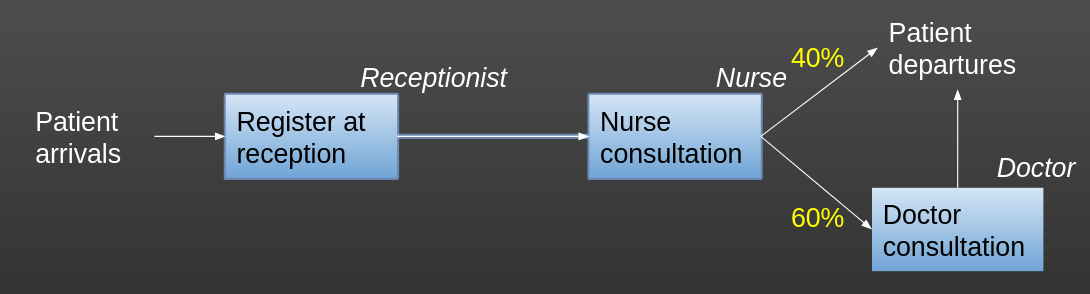
\includegraphics{images/example_simple_model_branching.png}

To model a branching path, we can use our good old Python friend
Conditional Logic.

Often, the branches in a DES are based on probabilities that represent
the proportion of patients (or whatever your entity is) that travel
along a certain route. For example, the data might show that 60\% of
patients see a doctor after seeing a nurse.

To model this, we can randomly sample from a uniform distribution
between 0 and 1, and compare the value to this probability. If we pick a
value below the probability, then we say that the patient follows this
route. Why does this work? Well\ldots{}

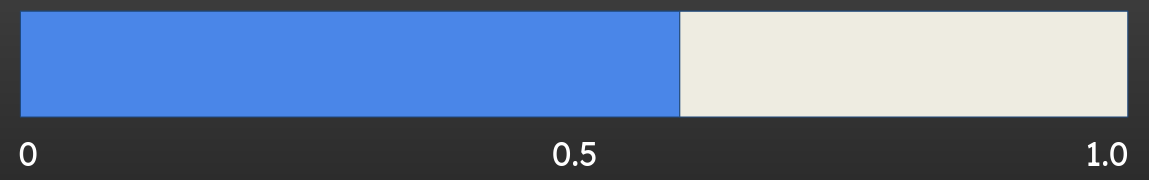
\includegraphics{images/probability_bar.png}

60\% of values between 0 and 1 are below 0.6.

Therefore, if there's an equal chance of any value being picked (as is
the case in a uniform distribution) then there's a 60\% probability of
picking one below 0.6.

\textbf{We can use this to emulate the probability of following a path.}

\begin{tcolorbox}[enhanced jigsaw, colframe=quarto-callout-note-color-frame, bottomtitle=1mm, breakable, rightrule=.15mm, coltitle=black, colbacktitle=quarto-callout-note-color!10!white, opacityback=0, leftrule=.75mm, arc=.35mm, toptitle=1mm, title=\textcolor{quarto-callout-note-color}{\faInfo}\hspace{0.5em}{Note}, titlerule=0mm, colback=white, toprule=.15mm, bottomrule=.15mm, left=2mm, opacitybacktitle=0.6]

Not all branching paths will be probability-based.

It may be that some paths are followed depending on - the time of day -
the type of patient - how long a patient spends in an activity - etc.

In these cases, you'd still use conditional logic, but just alter the
condition you're checking.

For the time of day, you'd want to check the current simulation time in
the run.

For the type of patient, you may have stored this in an
\textbf{attribute} of the patient.

\end{tcolorbox}

\begin{tcolorbox}[enhanced jigsaw, colframe=quarto-callout-tip-color-frame, bottomtitle=1mm, breakable, rightrule=.15mm, coltitle=black, colbacktitle=quarto-callout-tip-color!10!white, opacityback=0, leftrule=.75mm, arc=.35mm, toptitle=1mm, title=\textcolor{quarto-callout-tip-color}{\faLightbulb}\hspace{0.5em}{Tip}, titlerule=0mm, colback=white, toprule=.15mm, bottomrule=.15mm, left=2mm, opacitybacktitle=0.6]

Throughout the code, anything new that's been added will be followed by
the comment \texttt{\#\#NEW} - so look out for that in the following
code chunks.

\end{tcolorbox}

\section{Coding the model}\label{coding-the-model-1}

\subsection{the g class}\label{the-g-class-1}

We need to add a few additional parameters to our g class.

\begin{Shaded}
\begin{Highlighting}[]
\CommentTok{\# Class to store global parameter values.  We don\textquotesingle{}t create an instance of this}
\CommentTok{\# class {-} we just refer to the class blueprint itself to access the numbers}
\CommentTok{\# inside.}
\KeywordTok{class}\NormalTok{ g:}
\NormalTok{    patient\_inter }\OperatorTok{=} \DecValTok{5}
\NormalTok{    mean\_reception\_time }\OperatorTok{=} \DecValTok{2}
\NormalTok{    mean\_n\_consult\_time }\OperatorTok{=} \DecValTok{6}
\NormalTok{    mean\_d\_consult\_time }\OperatorTok{=} \DecValTok{20} \CommentTok{\#\#NEW}
\NormalTok{    number\_of\_receptionists }\OperatorTok{=} \DecValTok{1}
\NormalTok{    number\_of\_nurses }\OperatorTok{=} \DecValTok{1}
\NormalTok{    number\_of\_doctors }\OperatorTok{=} \DecValTok{2} \CommentTok{\#\#NEW}
\NormalTok{    prob\_seeing\_doctor }\OperatorTok{=} \FloatTok{0.6} \CommentTok{\#\#NEW}
\NormalTok{    sim\_duration }\OperatorTok{=} \DecValTok{120}
\NormalTok{    number\_of\_runs }\OperatorTok{=} \DecValTok{5}
\end{Highlighting}
\end{Shaded}

\subsection{The Patient class}\label{the-patient-class-1}

We want to add an additional attribute to record the time patients spend
with the doctor if they see one.

\begin{Shaded}
\begin{Highlighting}[]
\CommentTok{\# Class representing patients coming in to the clinic.}
\KeywordTok{class}\NormalTok{ Patient:}
    \KeywordTok{def} \FunctionTok{\_\_init\_\_}\NormalTok{(}\VariableTok{self}\NormalTok{, p\_id):}
        \VariableTok{self}\NormalTok{.}\BuiltInTok{id} \OperatorTok{=}\NormalTok{ p\_id}
        \VariableTok{self}\NormalTok{.q\_time\_recep }\OperatorTok{=} \DecValTok{0}
        \VariableTok{self}\NormalTok{.q\_time\_nurse }\OperatorTok{=} \DecValTok{0}
        \VariableTok{self}\NormalTok{.q\_time\_doctor }\OperatorTok{=} \DecValTok{0} \CommentTok{\#\#NEW}
\end{Highlighting}
\end{Shaded}

\subsection{The model class}\label{the-model-class-1}

\subsubsection{\texorpdfstring{the \textbf{init}
method}{the init method}}\label{the-init-method}

In the init method, we add a few additional atrributes to store
additional outputs from the model.

\begin{Shaded}
\begin{Highlighting}[]
\CommentTok{\# Class representing our model of the clinic.}
\KeywordTok{class}\NormalTok{ Model:}
    \CommentTok{\# Constructor to set up the model for a run.  We pass in a run number when}
    \CommentTok{\# we create a new model.}
    \KeywordTok{def} \FunctionTok{\_\_init\_\_}\NormalTok{(}\VariableTok{self}\NormalTok{, run\_number):}
        \CommentTok{\# Create a SimPy environment in which everything will live}
        \VariableTok{self}\NormalTok{.env }\OperatorTok{=}\NormalTok{ simpy.Environment()}

        \CommentTok{\# Create a patient counter (which we\textquotesingle{}ll use as a patient ID)}
        \VariableTok{self}\NormalTok{.patient\_counter }\OperatorTok{=} \DecValTok{0}

        \CommentTok{\# Create our resources}
        \VariableTok{self}\NormalTok{.receptionist }\OperatorTok{=}\NormalTok{ simpy.Resource(}
            \VariableTok{self}\NormalTok{.env, capacity}\OperatorTok{=}\NormalTok{g.number\_of\_receptionists}
\NormalTok{        )}
        \VariableTok{self}\NormalTok{.nurse }\OperatorTok{=}\NormalTok{ simpy.Resource(}\VariableTok{self}\NormalTok{.env, capacity}\OperatorTok{=}\NormalTok{g.number\_of\_nurses)}
        \VariableTok{self}\NormalTok{.doctor }\OperatorTok{=}\NormalTok{ simpy.Resource(}
            \VariableTok{self}\NormalTok{.env, capacity}\OperatorTok{=}\NormalTok{g.number\_of\_doctors) }\CommentTok{\#\#NEW}

        \CommentTok{\# Store the passed in run number}
        \VariableTok{self}\NormalTok{.run\_number }\OperatorTok{=}\NormalTok{ run\_number}

        \CommentTok{\# Create a new Pandas DataFrame that will store some results against}
        \CommentTok{\# the patient ID (which we\textquotesingle{}ll use as the index).}
        \VariableTok{self}\NormalTok{.results\_df }\OperatorTok{=}\NormalTok{ pd.DataFrame()}
        \VariableTok{self}\NormalTok{.results\_df[}\StringTok{"Patient ID"}\NormalTok{] }\OperatorTok{=}\NormalTok{ [}\DecValTok{1}\NormalTok{]}
        \VariableTok{self}\NormalTok{.results\_df[}\StringTok{"Q Time Recep"}\NormalTok{] }\OperatorTok{=}\NormalTok{ [}\FloatTok{0.0}\NormalTok{]}
        \VariableTok{self}\NormalTok{.results\_df[}\StringTok{"Time with Recep"}\NormalTok{] }\OperatorTok{=}\NormalTok{ [}\FloatTok{0.0}\NormalTok{]}
        \VariableTok{self}\NormalTok{.results\_df[}\StringTok{"Q Time Nurse"}\NormalTok{] }\OperatorTok{=}\NormalTok{ [}\FloatTok{0.0}\NormalTok{]}
        \VariableTok{self}\NormalTok{.results\_df[}\StringTok{"Time with Nurse"}\NormalTok{] }\OperatorTok{=}\NormalTok{ [}\FloatTok{0.0}\NormalTok{]}
        \VariableTok{self}\NormalTok{.results\_df[}\StringTok{"Q Time Doctor"}\NormalTok{] }\OperatorTok{=}\NormalTok{ [}\FloatTok{0.0}\NormalTok{] }\CommentTok{\#\#NEW}
        \VariableTok{self}\NormalTok{.results\_df[}\StringTok{"Time with Doctor"}\NormalTok{] }\OperatorTok{=}\NormalTok{ [}\FloatTok{0.0}\NormalTok{] }\CommentTok{\#\#NEW}
        \VariableTok{self}\NormalTok{.results\_df.set\_index(}\StringTok{"Patient ID"}\NormalTok{, inplace}\OperatorTok{=}\VariableTok{True}\NormalTok{)}

        \CommentTok{\# Create an attribute to store the mean queuing times across this run of}
        \CommentTok{\# the model}
        \VariableTok{self}\NormalTok{.mean\_q\_time\_recep }\OperatorTok{=} \DecValTok{0}
        \VariableTok{self}\NormalTok{.mean\_q\_time\_nurse }\OperatorTok{=} \DecValTok{0}
        \VariableTok{self}\NormalTok{.mean\_q\_time\_doctor }\OperatorTok{=} \DecValTok{0} \CommentTok{\#\#NEW}
\end{Highlighting}
\end{Shaded}

\subsubsection{The generator\_patient\_arrivals
method}\label{the-generator_patient_arrivals-method}

This method is unchanged.

\subsubsection{The attend\_clinic
method}\label{the-attend_clinic-method}

Here, we need to add in a chance of patients seeing the doctor on their
journey.

\begin{Shaded}
\begin{Highlighting}[]
\KeywordTok{def}\NormalTok{ attend\_clinic(}\VariableTok{self}\NormalTok{, patient):}
\NormalTok{        start\_q\_recep }\OperatorTok{=} \VariableTok{self}\NormalTok{.env.now}

        \ControlFlowTok{with} \VariableTok{self}\NormalTok{.receptionist.request() }\ImportTok{as}\NormalTok{ req:}
            \ControlFlowTok{yield}\NormalTok{ req}

\NormalTok{            end\_q\_recep }\OperatorTok{=} \VariableTok{self}\NormalTok{.env.now}

\NormalTok{            patient.q\_time\_recep }\OperatorTok{=}\NormalTok{ end\_q\_recep }\OperatorTok{{-}}\NormalTok{ start\_q\_recep}

\NormalTok{            sampled\_recep\_act\_time }\OperatorTok{=}\NormalTok{ random.expovariate(}
                \FloatTok{1.0} \OperatorTok{/}\NormalTok{ g.mean\_reception\_time}
\NormalTok{            )}

            \VariableTok{self}\NormalTok{.results\_df.at[patient.}\BuiltInTok{id}\NormalTok{, }\StringTok{"Q Time Recep"}\NormalTok{] }\OperatorTok{=}\NormalTok{ (}
\NormalTok{                 patient.q\_time\_recep}
\NormalTok{            )}
            \VariableTok{self}\NormalTok{.results\_df.at[patient.}\BuiltInTok{id}\NormalTok{, }\StringTok{"Time with Recep"}\NormalTok{] }\OperatorTok{=}\NormalTok{ (}
\NormalTok{                 sampled\_recep\_act\_time}
\NormalTok{            )}

            \ControlFlowTok{yield} \VariableTok{self}\NormalTok{.env.timeout(sampled\_recep\_act\_time)}

        \CommentTok{\# Here\textquotesingle{}s where the patient finishes with the receptionist, and starts}
        \CommentTok{\# queuing for the nurse}

\NormalTok{        start\_q\_nurse }\OperatorTok{=} \VariableTok{self}\NormalTok{.env.now}

        \ControlFlowTok{with} \VariableTok{self}\NormalTok{.nurse.request() }\ImportTok{as}\NormalTok{ req:}
            \ControlFlowTok{yield}\NormalTok{ req}

\NormalTok{            end\_q\_nurse }\OperatorTok{=} \VariableTok{self}\NormalTok{.env.now}

\NormalTok{            patient.q\_time\_nurse }\OperatorTok{=}\NormalTok{ end\_q\_nurse }\OperatorTok{{-}}\NormalTok{ start\_q\_nurse}

\NormalTok{            sampled\_nurse\_act\_time }\OperatorTok{=}\NormalTok{ random.expovariate(}\FloatTok{1.0} \OperatorTok{/}
\NormalTok{                                                        g.mean\_n\_consult\_time)}

            \VariableTok{self}\NormalTok{.results\_df.at[patient.}\BuiltInTok{id}\NormalTok{, }\StringTok{"Q Time Nurse"}\NormalTok{] }\OperatorTok{=}\NormalTok{ (}
\NormalTok{                patient.q\_time\_nurse)}
            \VariableTok{self}\NormalTok{.results\_df.at[patient.}\BuiltInTok{id}\NormalTok{, }\StringTok{"Time with Nurse"}\NormalTok{] }\OperatorTok{=}\NormalTok{ (}
\NormalTok{                sampled\_nurse\_act\_time)}

            \ControlFlowTok{yield} \VariableTok{self}\NormalTok{.env.timeout(sampled\_nurse\_act\_time)}

            \CommentTok{\# When the time above elapses, the generator function will return}
            \CommentTok{\# here.  As there\textquotesingle{}s nothing more that we\textquotesingle{}ve written, the function}
            \CommentTok{\# will simply end.  This is a sink.}

        \CommentTok{\#\#NEW}
        \CommentTok{\#\#}
        \CommentTok{\#\# {-}{-}{-}{-}{-}{-}{-}{-}{-}{-}{-}{-}{-}{-}{-}{-}{-}{-}{-}{-}{-}{-}{-}{-}{-}{-}{-}{-}{-}{-}{-}{-}{-}{-}{-}{-}{-}{-}{-}{-}{-}{-}{-}{-}{-}{-}{-}{-}{-}{-}{-}{-}{-}{-}{-}{-}{-}{-}{-}}
        \CommentTok{\#\# This is where our new code for seeing the doctor is}
        \CommentTok{\#\# We use conditional logic to determine whether the patient goes}
        \CommentTok{\#\# on to see the doctor or not}
        \CommentTok{\#\# {-}{-}{-}{-}{-}{-}{-}{-}{-}{-}{-}{-}{-}{-}{-}{-}{-}{-}{-}{-}{-}{-}{-}{-}{-}{-}{-}{-}{-}{-}{-}{-}{-}{-}{-}{-}{-}{-}{-}{-}{-}{-}{-}{-}{-}{-}{-}{-}{-}{-}{-}{-}{-}{-}{-}{-}{-}{-}{-}{-}}
        \CommentTok{\#}
        \CommentTok{\# We sample from the uniform distribution between 0 and 1.  If the value}
        \CommentTok{\# is less than the probability of seeing a doctor (stored in g Class)}
        \CommentTok{\# then we say the patient sees a doctor.}
        \CommentTok{\#}
        \CommentTok{\# If not, this block of code won\textquotesingle{}t be run and the patient will just}
        \CommentTok{\# leave the system (we could add in an else if we wanted a branching}
        \CommentTok{\# path to another activity instead)}

        \ControlFlowTok{if}\NormalTok{ random.uniform(}\DecValTok{0}\NormalTok{,}\DecValTok{1}\NormalTok{) }\OperatorTok{\textless{}}\NormalTok{ g.prob\_seeing\_doctor:}
\NormalTok{            start\_q\_doctor }\OperatorTok{=} \VariableTok{self}\NormalTok{.env.now}

            \ControlFlowTok{with} \VariableTok{self}\NormalTok{.doctor.request() }\ImportTok{as}\NormalTok{ req:}
                \ControlFlowTok{yield}\NormalTok{ req}

\NormalTok{                end\_q\_doctor }\OperatorTok{=} \VariableTok{self}\NormalTok{.env.now}

\NormalTok{                patient.q\_time\_doctor }\OperatorTok{=}\NormalTok{ end\_q\_doctor }\OperatorTok{{-}}\NormalTok{ start\_q\_doctor}

\NormalTok{                sampled\_doctor\_act\_time }\OperatorTok{=}\NormalTok{ random.expovariate(}
                    \FloatTok{1.0} \OperatorTok{/}\NormalTok{ g.mean\_d\_consult\_time}
\NormalTok{                )}

                \VariableTok{self}\NormalTok{.results\_df.at[patient.}\BuiltInTok{id}\NormalTok{, }\StringTok{"Q Time Doctor"}\NormalTok{] }\OperatorTok{=}\NormalTok{ (}
\NormalTok{                    patient.q\_time\_doctor}
\NormalTok{                )}
                \VariableTok{self}\NormalTok{.results\_df.at[patient.}\BuiltInTok{id}\NormalTok{, }\StringTok{"Time with Doctor"}\NormalTok{] }\OperatorTok{=}\NormalTok{ (}
\NormalTok{                    sampled\_doctor\_act\_time}
\NormalTok{                )}

                \ControlFlowTok{yield} \VariableTok{self}\NormalTok{.env.timeout(sampled\_doctor\_act\_time)}
\end{Highlighting}
\end{Shaded}

Let's try and understand a bit more about how we trigger the conditional
logic.

Let's look at the output of the line \texttt{random.uniform(0,1)}

\begin{Shaded}
\begin{Highlighting}[]
\NormalTok{random.uniform(}\DecValTok{0}\NormalTok{,}\DecValTok{1}\NormalTok{)}
\end{Highlighting}
\end{Shaded}

\begin{verbatim}
0.6394267984578837
\end{verbatim}

What about if we run it multiple times?

\begin{Shaded}
\begin{Highlighting}[]
\ControlFlowTok{for}\NormalTok{ i }\KeywordTok{in} \BuiltInTok{range}\NormalTok{(}\DecValTok{10}\NormalTok{):}
  \BuiltInTok{print}\NormalTok{(random.uniform(}\DecValTok{0}\NormalTok{,}\DecValTok{1}\NormalTok{))}
\end{Highlighting}
\end{Shaded}

\begin{verbatim}
0.025010755222666936
0.27502931836911926
0.22321073814882275
0.7364712141640124
0.6766994874229113
0.8921795677048454
0.08693883262941615
0.4219218196852704
0.029797219438070344
0.21863797480360336
\end{verbatim}

So how does this relate to our code?

In our g class, we set a probability threshold for patients being seen.
Let's pull that out:

\begin{Shaded}
\begin{Highlighting}[]
\BuiltInTok{print}\NormalTok{(g.prob\_seeing\_doctor)}
\end{Highlighting}
\end{Shaded}

\begin{verbatim}
0.6
\end{verbatim}

The code in the Model class tests whether the number generated by the
random number generator is below the threshold we've set of seeing the
doctor. If it is, the indented code where we actually see the doctor
will be run for that patient. If it is not, that bit is bypassed - which
in this case means they've reached the end of their journey and leave
the system (\textbf{a sink}).

\begin{Shaded}
\begin{Highlighting}[]
\ControlFlowTok{for}\NormalTok{ i }\KeywordTok{in} \BuiltInTok{range}\NormalTok{(}\DecValTok{10}\NormalTok{):}
\NormalTok{  random\_number }\OperatorTok{=}\NormalTok{ random.uniform(}\DecValTok{0}\NormalTok{,}\DecValTok{1}\NormalTok{)}
\NormalTok{  is\_below\_threshold }\OperatorTok{=}\NormalTok{ random\_number }\OperatorTok{\textless{}}\NormalTok{ g.prob\_seeing\_doctor}

  \ControlFlowTok{if}\NormalTok{ is\_below\_threshold:}
    \BuiltInTok{print}\NormalTok{(}\SpecialStringTok{f"Random number }\SpecialCharTok{\{}\NormalTok{random\_number}\SpecialCharTok{:.2f\}}\SpecialStringTok{ is LOWER than threshold (}\SpecialCharTok{\{}\NormalTok{g}\SpecialCharTok{.}\NormalTok{prob\_seeing\_doctor}\SpecialCharTok{\}}\SpecialStringTok{). "} \OperatorTok{+}
    \StringTok{"Doctor code is triggered."}\NormalTok{)}
  \ControlFlowTok{else}\NormalTok{:}
    \BuiltInTok{print}\NormalTok{(}\SpecialStringTok{f"Random number }\SpecialCharTok{\{}\NormalTok{random\_number}\SpecialCharTok{:.2f\}}\SpecialStringTok{ is HIGHER than threshold (}\SpecialCharTok{\{}\NormalTok{g}\SpecialCharTok{.}\NormalTok{prob\_seeing\_doctor}\SpecialCharTok{\}}\SpecialStringTok{). "} \OperatorTok{+}
    \StringTok{"Doctor code is **not** triggered."}\NormalTok{)}
\end{Highlighting}
\end{Shaded}

\begin{verbatim}
Random number 0.51 is LOWER than threshold (0.6). Doctor code is triggered.
Random number 0.03 is LOWER than threshold (0.6). Doctor code is triggered.
Random number 0.20 is LOWER than threshold (0.6). Doctor code is triggered.
Random number 0.65 is HIGHER than threshold (0.6). Doctor code is **not** triggered.
Random number 0.54 is LOWER than threshold (0.6). Doctor code is triggered.
Random number 0.22 is LOWER than threshold (0.6). Doctor code is triggered.
Random number 0.59 is LOWER than threshold (0.6). Doctor code is triggered.
Random number 0.81 is HIGHER than threshold (0.6). Doctor code is **not** triggered.
Random number 0.01 is LOWER than threshold (0.6). Doctor code is triggered.
Random number 0.81 is HIGHER than threshold (0.6). Doctor code is **not** triggered.
\end{verbatim}

If we run this code a hundred thousand times and plot the results, we
can start to see the pattern emerging despite the random element of the
number generator.

\begin{Shaded}
\begin{Highlighting}[]
\ImportTok{import}\NormalTok{ plotly.express }\ImportTok{as}\NormalTok{ px}
\ImportTok{import}\NormalTok{ pandas }\ImportTok{as}\NormalTok{ pd}
\ImportTok{import}\NormalTok{ numpy }\ImportTok{as}\NormalTok{ np}

\NormalTok{random\_vals }\OperatorTok{=}\NormalTok{ [random.uniform(}\DecValTok{0}\NormalTok{,}\DecValTok{1}\NormalTok{) }\ControlFlowTok{for}\NormalTok{ i }\KeywordTok{in} \BuiltInTok{range}\NormalTok{(}\DecValTok{100000}\NormalTok{)]}

\NormalTok{random\_vals\_df }\OperatorTok{=}\NormalTok{ pd.DataFrame(\{}\StringTok{"value"}\NormalTok{ :random\_vals\})}

\NormalTok{random\_vals\_df[}\StringTok{\textquotesingle{}threshold\textquotesingle{}}\NormalTok{] }\OperatorTok{=}\NormalTok{ np.where(random\_vals\_df[}\StringTok{"value"}\NormalTok{]}\OperatorTok{\textless{}}\FloatTok{0.6}\NormalTok{, }\StringTok{\textquotesingle{}below\textquotesingle{}}\NormalTok{, }\StringTok{\textquotesingle{}above\textquotesingle{}}\NormalTok{)}

\NormalTok{fig }\OperatorTok{=}\NormalTok{ px.histogram(random\_vals\_df, color}\OperatorTok{=}\StringTok{"threshold"}\NormalTok{)}

\NormalTok{fig.update\_traces(xbins}\OperatorTok{=}\BuiltInTok{dict}\NormalTok{(}
\NormalTok{        start}\OperatorTok{=}\FloatTok{0.0}\NormalTok{,}
\NormalTok{        end}\OperatorTok{=}\FloatTok{1.0}\NormalTok{,}
\NormalTok{        size}\OperatorTok{=}\FloatTok{0.1}
\NormalTok{    ),}
\NormalTok{    marker\_line\_width}\OperatorTok{=}\DecValTok{1}\NormalTok{,marker\_line\_color}\OperatorTok{=}\StringTok{"black"}\NormalTok{)}


\NormalTok{fig.show()}
\end{Highlighting}
\end{Shaded}

\begin{verbatim}
Unable to display output for mime type(s): text/html
\end{verbatim}

\begin{verbatim}
Unable to display output for mime type(s): application/vnd.plotly.v1+json, text/html
\end{verbatim}

So for every 1000 patients, \emph{roughly} 600 will see a doctor, and
\emph{roughly} 400 will leave the system straight after seeing the
nurse.

\subsubsection{The calculate\_run\_results
method}\label{the-calculate_run_results-method}

In this method, we just add an additional step to measure the mean time
spent queueing for a doctor across all patients in this run.

\begin{Shaded}
\begin{Highlighting}[]
\CommentTok{\# This method calculates results over a single run.  Here we just calculate}
\CommentTok{\# a mean, but in real world models you\textquotesingle{}d probably want to calculate more.}
\KeywordTok{def}\NormalTok{ calculate\_run\_results(}\VariableTok{self}\NormalTok{):}
    \CommentTok{\# Take the mean of the queuing times across patients in this run of the}
    \CommentTok{\# model.}
    \VariableTok{self}\NormalTok{.mean\_q\_time\_recep }\OperatorTok{=} \VariableTok{self}\NormalTok{.results\_df[}\StringTok{"Q Time Recep"}\NormalTok{].mean()}
    \VariableTok{self}\NormalTok{.mean\_q\_time\_nurse }\OperatorTok{=} \VariableTok{self}\NormalTok{.results\_df[}\StringTok{"Q Time Nurse"}\NormalTok{].mean()}
    \VariableTok{self}\NormalTok{.mean\_q\_time\_doctor }\OperatorTok{=} \VariableTok{self}\NormalTok{.results\_df[}\StringTok{"Q Time Doctor"}\NormalTok{].mean() }\CommentTok{\#\#NEW}
\end{Highlighting}
\end{Shaded}

\subsubsection{The run method}\label{the-run-method}

The run method is unchanged

\subsection{The trial class}\label{the-trial-class-1}

\subsubsection{\texorpdfstring{The \textbf{init}
method}{The init method}}\label{the-init-method-1}

In the init method, we just add a placeholder for measuring the mean
queue time of a doctor.

\begin{Shaded}
\begin{Highlighting}[]
\KeywordTok{def}  \FunctionTok{\_\_init\_\_}\NormalTok{(}\VariableTok{self}\NormalTok{):}
    \VariableTok{self}\NormalTok{.df\_trial\_results }\OperatorTok{=}\NormalTok{ pd.DataFrame()}
    \VariableTok{self}\NormalTok{.df\_trial\_results[}\StringTok{"Run Number"}\NormalTok{] }\OperatorTok{=}\NormalTok{ [}\DecValTok{0}\NormalTok{]}
    \VariableTok{self}\NormalTok{.df\_trial\_results[}\StringTok{"Mean Q Time Recep"}\NormalTok{] }\OperatorTok{=}\NormalTok{ [}\FloatTok{0.0}\NormalTok{]}
    \VariableTok{self}\NormalTok{.df\_trial\_results[}\StringTok{"Mean Q Time Nurse"}\NormalTok{] }\OperatorTok{=}\NormalTok{ [}\FloatTok{0.0}\NormalTok{]}
    \VariableTok{self}\NormalTok{.df\_trial\_results[}\StringTok{"Mean Q Time Doctor"}\NormalTok{] }\OperatorTok{=}\NormalTok{ [}\FloatTok{0.0}\NormalTok{] }\CommentTok{\#\#NEW}
    \VariableTok{self}\NormalTok{.df\_trial\_results.set\_index(}\StringTok{"Run Number"}\NormalTok{, inplace}\OperatorTok{=}\VariableTok{True}\NormalTok{)}
\end{Highlighting}
\end{Shaded}

\subsubsection{The run\_trial method}\label{the-run_trial-method}

Here, we just add in the mean queue time for the doctor to the trial
results dataframe.

\begin{Shaded}
\begin{Highlighting}[]
  \KeywordTok{def}\NormalTok{ run\_trial(}\VariableTok{self}\NormalTok{):}
      \CommentTok{\# Run the simulation for the number of runs specified in g class.}
      \CommentTok{\# For each run, we create a new instance of the Model class and call its}
      \CommentTok{\# run method, which sets everything else in motion.  Once the run has}
      \CommentTok{\# completed, we grab out the stored run results (just mean queuing time}
      \CommentTok{\# here) and store it against the run number in the trial results}
      \CommentTok{\# dataframe.}
      \ControlFlowTok{for}\NormalTok{ run }\KeywordTok{in} \BuiltInTok{range}\NormalTok{(g.number\_of\_runs):}
\NormalTok{          my\_model }\OperatorTok{=}\NormalTok{ Model(run)}
\NormalTok{          my\_model.run()}

          \CommentTok{\#\#NEW {-} added mean queue time for doctor to end of list}
          \VariableTok{self}\NormalTok{.df\_trial\_results.loc[run] }\OperatorTok{=}\NormalTok{ [my\_model.mean\_q\_time\_recep,}
\NormalTok{                                            my\_model.mean\_q\_time\_nurse,}
\NormalTok{                                            my\_model.mean\_q\_time\_doctor]}

      \CommentTok{\# Once the trial (ie all runs) has completed, print the final results}
      \VariableTok{self}\NormalTok{.print\_trial\_results()}
\end{Highlighting}
\end{Shaded}

\section{Evaluating the outputs}\label{evaluating-the-outputs-1}

Below is the full updated code for this model.

\begin{tcolorbox}[enhanced jigsaw, colframe=quarto-callout-note-color-frame, bottomtitle=1mm, breakable, rightrule=.15mm, coltitle=black, colbacktitle=quarto-callout-note-color!10!white, opacityback=0, leftrule=.75mm, arc=.35mm, toptitle=1mm, title=\textcolor{quarto-callout-note-color}{\faInfo}\hspace{0.5em}{Click here to view the code}, titlerule=0mm, colback=white, toprule=.15mm, bottomrule=.15mm, left=2mm, opacitybacktitle=0.6]

\begin{Shaded}
\begin{Highlighting}[]
\ImportTok{import}\NormalTok{ simpy}
\ImportTok{import}\NormalTok{ random}
\ImportTok{import}\NormalTok{ pandas }\ImportTok{as}\NormalTok{ pd}

\CommentTok{\# Class to store global parameter values.  We don\textquotesingle{}t create an instance of this}
\CommentTok{\# class {-} we just refer to the class blueprint itself to access the numbers}
\CommentTok{\# inside.}
\KeywordTok{class}\NormalTok{ g:}
\NormalTok{    patient\_inter }\OperatorTok{=} \DecValTok{5}
\NormalTok{    mean\_reception\_time }\OperatorTok{=} \DecValTok{2}
\NormalTok{    mean\_n\_consult\_time }\OperatorTok{=} \DecValTok{6}
\NormalTok{    mean\_d\_consult\_time }\OperatorTok{=} \DecValTok{20} \CommentTok{\#\#NEW}
\NormalTok{    number\_of\_receptionists }\OperatorTok{=} \DecValTok{1}
\NormalTok{    number\_of\_nurses }\OperatorTok{=} \DecValTok{1}
\NormalTok{    number\_of\_doctors }\OperatorTok{=} \DecValTok{2} \CommentTok{\#\#NEW}
\NormalTok{    prob\_seeing\_doctor }\OperatorTok{=} \FloatTok{0.6} \CommentTok{\#\#NEW}
\NormalTok{    sim\_duration }\OperatorTok{=} \DecValTok{120}
\NormalTok{    number\_of\_runs }\OperatorTok{=} \DecValTok{1}

\CommentTok{\# Class representing patients coming in to the clinic.}
\KeywordTok{class}\NormalTok{ Patient:}
    \KeywordTok{def} \FunctionTok{\_\_init\_\_}\NormalTok{(}\VariableTok{self}\NormalTok{, p\_id):}
        \VariableTok{self}\NormalTok{.}\BuiltInTok{id} \OperatorTok{=}\NormalTok{ p\_id}
        \VariableTok{self}\NormalTok{.q\_time\_recep }\OperatorTok{=} \DecValTok{0}
        \VariableTok{self}\NormalTok{.q\_time\_nurse }\OperatorTok{=} \DecValTok{0}
        \VariableTok{self}\NormalTok{.q\_time\_doctor }\OperatorTok{=} \DecValTok{0} \CommentTok{\#\#NEW}

\CommentTok{\# Class representing our model of the clinic.}
\KeywordTok{class}\NormalTok{ Model:}
    \CommentTok{\# Constructor to set up the model for a run.  We pass in a run number when}
    \CommentTok{\# we create a new model.}
    \KeywordTok{def} \FunctionTok{\_\_init\_\_}\NormalTok{(}\VariableTok{self}\NormalTok{, run\_number):}
        \CommentTok{\# Create a SimPy environment in which everything will live}
        \VariableTok{self}\NormalTok{.env }\OperatorTok{=}\NormalTok{ simpy.Environment()}

        \CommentTok{\# Create a patient counter (which we\textquotesingle{}ll use as a patient ID)}
        \VariableTok{self}\NormalTok{.patient\_counter }\OperatorTok{=} \DecValTok{0}

        \CommentTok{\# Create our resources}
        \VariableTok{self}\NormalTok{.receptionist }\OperatorTok{=}\NormalTok{ simpy.Resource(}
            \VariableTok{self}\NormalTok{.env, capacity}\OperatorTok{=}\NormalTok{g.number\_of\_receptionists}
\NormalTok{        )}
        \VariableTok{self}\NormalTok{.nurse }\OperatorTok{=}\NormalTok{ simpy.Resource(}\VariableTok{self}\NormalTok{.env, capacity}\OperatorTok{=}\NormalTok{g.number\_of\_nurses)}
        \VariableTok{self}\NormalTok{.doctor }\OperatorTok{=}\NormalTok{ simpy.Resource(}
            \VariableTok{self}\NormalTok{.env, capacity}\OperatorTok{=}\NormalTok{g.number\_of\_doctors) }\CommentTok{\#\#NEW}

        \CommentTok{\# Store the passed in run number}
        \VariableTok{self}\NormalTok{.run\_number }\OperatorTok{=}\NormalTok{ run\_number}

        \CommentTok{\# Create a new Pandas DataFrame that will store some results against}
        \CommentTok{\# the patient ID (which we\textquotesingle{}ll use as the index).}
        \VariableTok{self}\NormalTok{.results\_df }\OperatorTok{=}\NormalTok{ pd.DataFrame()}
        \VariableTok{self}\NormalTok{.results\_df[}\StringTok{"Patient ID"}\NormalTok{] }\OperatorTok{=}\NormalTok{ [}\DecValTok{1}\NormalTok{]}
        \VariableTok{self}\NormalTok{.results\_df[}\StringTok{"Q Time Recep"}\NormalTok{] }\OperatorTok{=}\NormalTok{ [}\FloatTok{0.0}\NormalTok{]}
        \VariableTok{self}\NormalTok{.results\_df[}\StringTok{"Time with Recep"}\NormalTok{] }\OperatorTok{=}\NormalTok{ [}\FloatTok{0.0}\NormalTok{]}
        \VariableTok{self}\NormalTok{.results\_df[}\StringTok{"Q Time Nurse"}\NormalTok{] }\OperatorTok{=}\NormalTok{ [}\FloatTok{0.0}\NormalTok{]}
        \VariableTok{self}\NormalTok{.results\_df[}\StringTok{"Time with Nurse"}\NormalTok{] }\OperatorTok{=}\NormalTok{ [}\FloatTok{0.0}\NormalTok{]}
        \VariableTok{self}\NormalTok{.results\_df[}\StringTok{"Q Time Doctor"}\NormalTok{] }\OperatorTok{=}\NormalTok{ [}\FloatTok{0.0}\NormalTok{] }\CommentTok{\#\#NEW}
        \VariableTok{self}\NormalTok{.results\_df[}\StringTok{"Time with Doctor"}\NormalTok{] }\OperatorTok{=}\NormalTok{ [}\FloatTok{0.0}\NormalTok{] }\CommentTok{\#\#NEW}
        \VariableTok{self}\NormalTok{.results\_df.set\_index(}\StringTok{"Patient ID"}\NormalTok{, inplace}\OperatorTok{=}\VariableTok{True}\NormalTok{)}

        \CommentTok{\# Create an attribute to store the mean queuing times across this run of}
        \CommentTok{\# the model}
        \VariableTok{self}\NormalTok{.mean\_q\_time\_recep }\OperatorTok{=} \DecValTok{0}
        \VariableTok{self}\NormalTok{.mean\_q\_time\_nurse }\OperatorTok{=} \DecValTok{0}
        \VariableTok{self}\NormalTok{.mean\_q\_time\_doctor }\OperatorTok{=} \DecValTok{0} \CommentTok{\#\#NEW}

    \CommentTok{\# A generator function that represents the DES generator for patient}
    \CommentTok{\# arrivals}
    \KeywordTok{def}\NormalTok{ generator\_patient\_arrivals(}\VariableTok{self}\NormalTok{):}
        \CommentTok{\# We use an infinite loop here to keep doing this indefinitely whilst}
        \CommentTok{\# the simulation runs}
        \ControlFlowTok{while} \VariableTok{True}\NormalTok{:}
            \CommentTok{\# Increment the patient counter by 1 (this means our first patient}
            \CommentTok{\# will have an ID of 1)}
            \VariableTok{self}\NormalTok{.patient\_counter }\OperatorTok{+=} \DecValTok{1}

            \CommentTok{\# Create a new patient {-} an instance of the Patient Class we}
            \CommentTok{\# defined above.  Remember, we pass in the ID when creating a}
            \CommentTok{\# patient {-} so here we pass the patient counter to use as the ID.}
\NormalTok{            p }\OperatorTok{=}\NormalTok{ Patient(}\VariableTok{self}\NormalTok{.patient\_counter)}

            \CommentTok{\# Tell SimPy to start up the attend\_clinic generator function with}
            \CommentTok{\# this patient (the generator function that will model the}
            \CommentTok{\# patient\textquotesingle{}s journey through the system)}
            \VariableTok{self}\NormalTok{.env.process(}\VariableTok{self}\NormalTok{.attend\_clinic(p))}

            \CommentTok{\# Randomly sample the time to the next patient arriving.  Here, we}
            \CommentTok{\# sample from an exponential distribution (common for inter{-}arrival}
            \CommentTok{\# times), and pass in a lambda value of 1 / mean.  The mean}
            \CommentTok{\# inter{-}arrival time is stored in the g class.}
\NormalTok{            sampled\_inter }\OperatorTok{=}\NormalTok{ random.expovariate(}\FloatTok{1.0} \OperatorTok{/}\NormalTok{ g.patient\_inter)}

            \CommentTok{\# Freeze this instance of this function in place until the}
            \CommentTok{\# inter{-}arrival time we sampled above has elapsed.  Note {-} time in}
            \CommentTok{\# SimPy progresses in "Time Units", which can represent anything}
            \CommentTok{\# you like (just make sure you\textquotesingle{}re consistent within the model)}
            \ControlFlowTok{yield} \VariableTok{self}\NormalTok{.env.timeout(sampled\_inter)}

    \CommentTok{\# A generator function that represents the pathway for a patient going}
    \CommentTok{\# through the clinic.}
    \CommentTok{\# The patient object is passed in to the generator function so we can}
    \CommentTok{\# extract information from / record information to it}
    \KeywordTok{def}\NormalTok{ attend\_clinic(}\VariableTok{self}\NormalTok{, patient):}
\NormalTok{        start\_q\_recep }\OperatorTok{=} \VariableTok{self}\NormalTok{.env.now}

        \ControlFlowTok{with} \VariableTok{self}\NormalTok{.receptionist.request() }\ImportTok{as}\NormalTok{ req:}
            \ControlFlowTok{yield}\NormalTok{ req}

\NormalTok{            end\_q\_recep }\OperatorTok{=} \VariableTok{self}\NormalTok{.env.now}

\NormalTok{            patient.q\_time\_recep }\OperatorTok{=}\NormalTok{ end\_q\_recep }\OperatorTok{{-}}\NormalTok{ start\_q\_recep}

\NormalTok{            sampled\_recep\_act\_time }\OperatorTok{=}\NormalTok{ random.expovariate(}
                \FloatTok{1.0} \OperatorTok{/}\NormalTok{ g.mean\_reception\_time}
\NormalTok{            )}

            \VariableTok{self}\NormalTok{.results\_df.at[patient.}\BuiltInTok{id}\NormalTok{, }\StringTok{"Q Time Recep"}\NormalTok{] }\OperatorTok{=}\NormalTok{ (}
\NormalTok{                 patient.q\_time\_recep}
\NormalTok{            )}
            \VariableTok{self}\NormalTok{.results\_df.at[patient.}\BuiltInTok{id}\NormalTok{, }\StringTok{"Time with Recep"}\NormalTok{] }\OperatorTok{=}\NormalTok{ (}
\NormalTok{                 sampled\_recep\_act\_time}
\NormalTok{            )}

            \ControlFlowTok{yield} \VariableTok{self}\NormalTok{.env.timeout(sampled\_recep\_act\_time)}

        \CommentTok{\# Here\textquotesingle{}s where the patient finishes with the receptionist, and starts}
        \CommentTok{\# queuing for the nurse}

        \CommentTok{\# Record the time the patient started queuing for a nurse}
\NormalTok{        start\_q\_nurse }\OperatorTok{=} \VariableTok{self}\NormalTok{.env.now}

        \CommentTok{\# This code says request a nurse resource, and do all of the following}
        \CommentTok{\# block of code with that nurse resource held in place (and therefore}
        \CommentTok{\# not usable by another patient)}
        \ControlFlowTok{with} \VariableTok{self}\NormalTok{.nurse.request() }\ImportTok{as}\NormalTok{ req:}
            \CommentTok{\# Freeze the function until the request for a nurse can be met.}
            \CommentTok{\# The patient is currently queuing.}
            \ControlFlowTok{yield}\NormalTok{ req}

            \CommentTok{\# When we get to this bit of code, control has been passed back to}
            \CommentTok{\# the generator function, and therefore the request for a nurse has}
            \CommentTok{\# been met.  We now have the nurse, and have stopped queuing, so we}
            \CommentTok{\# can record the current time as the time we finished queuing.}
\NormalTok{            end\_q\_nurse }\OperatorTok{=} \VariableTok{self}\NormalTok{.env.now}

            \CommentTok{\# Calculate the time this patient was queuing for the nurse, and}
            \CommentTok{\# record it in the patient\textquotesingle{}s attribute for this.}
\NormalTok{            patient.q\_time\_nurse }\OperatorTok{=}\NormalTok{ end\_q\_nurse }\OperatorTok{{-}}\NormalTok{ start\_q\_nurse}

            \CommentTok{\# Now we\textquotesingle{}ll randomly sample the time this patient with the nurse.}
            \CommentTok{\# Here, we use an Exponential distribution for simplicity, but you}
            \CommentTok{\# would typically use a Log Normal distribution for a real model}
            \CommentTok{\# (we\textquotesingle{}ll come back to that).  As with sampling the inter{-}arrival}
            \CommentTok{\# times, we grab the mean from the g class, and pass in 1 / mean}
            \CommentTok{\# as the lambda value.}
\NormalTok{            sampled\_nurse\_act\_time }\OperatorTok{=}\NormalTok{ random.expovariate(}\FloatTok{1.0} \OperatorTok{/}
\NormalTok{                                                        g.mean\_n\_consult\_time)}

            \CommentTok{\# Here we\textquotesingle{}ll store the queuing time for the nurse and the sampled}
            \CommentTok{\# time to spend with the nurse in the results DataFrame against the}
            \CommentTok{\# ID for this patient.  In real world models, you may not want to}
            \CommentTok{\# bother storing the sampled activity times {-} but as this is a}
            \CommentTok{\# simple model, we\textquotesingle{}ll do it here.}
            \CommentTok{\# We use a handy property of pandas called .at, which works a bit}
            \CommentTok{\# like .loc.  .at allows us to access (and therefore change) a}
            \CommentTok{\# particular cell in our DataFrame by providing the row and column.}
            \CommentTok{\# Here, we specify the row as the patient ID (the index), and the}
            \CommentTok{\# column for the value we want to update for that patient.}
            \VariableTok{self}\NormalTok{.results\_df.at[patient.}\BuiltInTok{id}\NormalTok{, }\StringTok{"Q Time Nurse"}\NormalTok{] }\OperatorTok{=}\NormalTok{ (}
\NormalTok{                patient.q\_time\_nurse)}
            \VariableTok{self}\NormalTok{.results\_df.at[patient.}\BuiltInTok{id}\NormalTok{, }\StringTok{"Time with Nurse"}\NormalTok{] }\OperatorTok{=}\NormalTok{ (}
\NormalTok{                sampled\_nurse\_act\_time)}

            \CommentTok{\# Freeze this function in place for the activity time we sampled}
            \CommentTok{\# above.  This is the patient spending time with the nurse.}
            \ControlFlowTok{yield} \VariableTok{self}\NormalTok{.env.timeout(sampled\_nurse\_act\_time)}

            \CommentTok{\# When the time above elapses, the generator function will return}
            \CommentTok{\# here.  As there\textquotesingle{}s nothing more that we\textquotesingle{}ve written, the function}
            \CommentTok{\# will simply end.  This is a sink.  We could choose to add}
            \CommentTok{\# something here if we wanted to record something {-} e.g. a counter}
            \CommentTok{\# for number of patients that left, recording something about the}
            \CommentTok{\# patients that left at a particular sink etc.}

        \CommentTok{\#\#NEW added conditional logic to see if patient goes on to see doctor}
        \CommentTok{\# We sample from the uniform distribution between 0 and 1.  If the value}
        \CommentTok{\# is less than the probability of seeing a doctor (stored in g Class)}
        \CommentTok{\# then we say the patient sees a doctor.}
        \CommentTok{\# If not, this block of code won\textquotesingle{}t be run and the patient will just}
        \CommentTok{\# leave the system (we could add in an else if we wanted a branching}
        \CommentTok{\# path to another activity instead)}
        \ControlFlowTok{if}\NormalTok{ random.uniform(}\DecValTok{0}\NormalTok{,}\DecValTok{1}\NormalTok{) }\OperatorTok{\textless{}}\NormalTok{ g.prob\_seeing\_doctor:}
\NormalTok{            start\_q\_doctor }\OperatorTok{=} \VariableTok{self}\NormalTok{.env.now}

            \ControlFlowTok{with} \VariableTok{self}\NormalTok{.doctor.request() }\ImportTok{as}\NormalTok{ req:}
                \ControlFlowTok{yield}\NormalTok{ req}

\NormalTok{                end\_q\_doctor }\OperatorTok{=} \VariableTok{self}\NormalTok{.env.now}

\NormalTok{                patient.q\_time\_doctor }\OperatorTok{=}\NormalTok{ end\_q\_doctor }\OperatorTok{{-}}\NormalTok{ start\_q\_doctor}

\NormalTok{                sampled\_doctor\_act\_time }\OperatorTok{=}\NormalTok{ random.expovariate(}
                    \FloatTok{1.0} \OperatorTok{/}\NormalTok{ g.mean\_d\_consult\_time}
\NormalTok{                )}

                \VariableTok{self}\NormalTok{.results\_df.at[patient.}\BuiltInTok{id}\NormalTok{, }\StringTok{"Q Time Doctor"}\NormalTok{] }\OperatorTok{=}\NormalTok{ (}
\NormalTok{                    patient.q\_time\_doctor}
\NormalTok{                )}
                \VariableTok{self}\NormalTok{.results\_df.at[patient.}\BuiltInTok{id}\NormalTok{, }\StringTok{"Time with Doctor"}\NormalTok{] }\OperatorTok{=}\NormalTok{ (}
\NormalTok{                    sampled\_doctor\_act\_time}
\NormalTok{                )}

                \ControlFlowTok{yield} \VariableTok{self}\NormalTok{.env.timeout(sampled\_doctor\_act\_time)}

    \CommentTok{\# This method calculates results over a single run.  Here we just calculate}
    \CommentTok{\# a mean, but in real world models you\textquotesingle{}d probably want to calculate more.}
    \KeywordTok{def}\NormalTok{ calculate\_run\_results(}\VariableTok{self}\NormalTok{):}
        \CommentTok{\# Take the mean of the queuing times across patients in this run of the}
        \CommentTok{\# model.}
        \VariableTok{self}\NormalTok{.mean\_q\_time\_recep }\OperatorTok{=} \VariableTok{self}\NormalTok{.results\_df[}\StringTok{"Q Time Recep"}\NormalTok{].mean()}
        \VariableTok{self}\NormalTok{.mean\_q\_time\_nurse }\OperatorTok{=} \VariableTok{self}\NormalTok{.results\_df[}\StringTok{"Q Time Nurse"}\NormalTok{].mean()}
        \VariableTok{self}\NormalTok{.mean\_q\_time\_doctor }\OperatorTok{=} \VariableTok{self}\NormalTok{.results\_df[}\StringTok{"Q Time Doctor"}\NormalTok{].mean() }\CommentTok{\#\#NEW}

    \CommentTok{\# The run method starts up the DES entity generators, runs the simulation,}
    \CommentTok{\# and in turns calls anything we need to generate results for the run}
    \KeywordTok{def}\NormalTok{ run(}\VariableTok{self}\NormalTok{):}
        \CommentTok{\# Start up our DES entity generators that create new patients.  We\textquotesingle{}ve}
        \CommentTok{\# only got one in this model, but we\textquotesingle{}d need to do this for each one if}
        \CommentTok{\# we had multiple generators.}
        \VariableTok{self}\NormalTok{.env.process(}\VariableTok{self}\NormalTok{.generator\_patient\_arrivals())}

        \CommentTok{\# Run the model for the duration specified in g class}
        \VariableTok{self}\NormalTok{.env.run(until}\OperatorTok{=}\NormalTok{g.sim\_duration)}

        \CommentTok{\# Now the simulation run has finished, call the method that calculates}
        \CommentTok{\# run results}
        \VariableTok{self}\NormalTok{.calculate\_run\_results()}

        \CommentTok{\# Print the run number with the patient{-}level results from this run of}
        \CommentTok{\# the model}
        \BuiltInTok{print}\NormalTok{ (}\SpecialStringTok{f"Run Number }\SpecialCharTok{\{}\VariableTok{self}\SpecialCharTok{.}\NormalTok{run\_number}\SpecialCharTok{\}}\SpecialStringTok{"}\NormalTok{)}
        \BuiltInTok{print}\NormalTok{ (}\VariableTok{self}\NormalTok{.results\_df)}

\CommentTok{\# Class representing a Trial for our simulation {-} a batch of simulation runs.}
\KeywordTok{class}\NormalTok{ Trial:}
    \CommentTok{\# The constructor sets up a pandas dataframe that will store the key}
    \CommentTok{\# results from each run against run number, with run number as the index.}
    \KeywordTok{def}  \FunctionTok{\_\_init\_\_}\NormalTok{(}\VariableTok{self}\NormalTok{):}
        \VariableTok{self}\NormalTok{.df\_trial\_results }\OperatorTok{=}\NormalTok{ pd.DataFrame()}
        \VariableTok{self}\NormalTok{.df\_trial\_results[}\StringTok{"Run Number"}\NormalTok{] }\OperatorTok{=}\NormalTok{ [}\DecValTok{0}\NormalTok{]}
        \VariableTok{self}\NormalTok{.df\_trial\_results[}\StringTok{"Mean Q Time Recep"}\NormalTok{] }\OperatorTok{=}\NormalTok{ [}\FloatTok{0.0}\NormalTok{]}
        \VariableTok{self}\NormalTok{.df\_trial\_results[}\StringTok{"Mean Q Time Nurse"}\NormalTok{] }\OperatorTok{=}\NormalTok{ [}\FloatTok{0.0}\NormalTok{]}
        \VariableTok{self}\NormalTok{.df\_trial\_results[}\StringTok{"Mean Q Time Doctor"}\NormalTok{] }\OperatorTok{=}\NormalTok{ [}\FloatTok{0.0}\NormalTok{] }\CommentTok{\#\#NEW}
        \VariableTok{self}\NormalTok{.df\_trial\_results.set\_index(}\StringTok{"Run Number"}\NormalTok{, inplace}\OperatorTok{=}\VariableTok{True}\NormalTok{)}

    \CommentTok{\# Method to print out the results from the trial.  In real world models,}
    \CommentTok{\# you\textquotesingle{}d likely save them as well as (or instead of) printing them}
    \KeywordTok{def}\NormalTok{ print\_trial\_results(}\VariableTok{self}\NormalTok{):}
        \BuiltInTok{print}\NormalTok{ (}\StringTok{"Trial Results"}\NormalTok{)}
        \BuiltInTok{print}\NormalTok{ (}\VariableTok{self}\NormalTok{.df\_trial\_results)}

    \CommentTok{\# Method to run a trial}
    \KeywordTok{def}\NormalTok{ run\_trial(}\VariableTok{self}\NormalTok{):}
        \CommentTok{\# Run the simulation for the number of runs specified in g class.}
        \CommentTok{\# For each run, we create a new instance of the Model class and call its}
        \CommentTok{\# run method, which sets everything else in motion.  Once the run has}
        \CommentTok{\# completed, we grab out the stored run results (just mean queuing time}
        \CommentTok{\# here) and store it against the run number in the trial results}
        \CommentTok{\# dataframe.}
        \ControlFlowTok{for}\NormalTok{ run }\KeywordTok{in} \BuiltInTok{range}\NormalTok{(g.number\_of\_runs):}
\NormalTok{            my\_model }\OperatorTok{=}\NormalTok{ Model(run)}
\NormalTok{            my\_model.run()}

            \CommentTok{\#\#NEW {-} added mean queue time for doctor to end of list}
            \VariableTok{self}\NormalTok{.df\_trial\_results.loc[run] }\OperatorTok{=}\NormalTok{ [my\_model.mean\_q\_time\_recep,}
\NormalTok{                                              my\_model.mean\_q\_time\_nurse,}
\NormalTok{                                              my\_model.mean\_q\_time\_doctor]}

        \CommentTok{\# Once the trial (ie all runs) has completed, print the final results}
        \VariableTok{self}\NormalTok{.print\_trial\_results()}
\end{Highlighting}
\end{Shaded}

\end{tcolorbox}

Let's look at the outputs for a single run.

When a patient doesn't see a doctor, notice that their value for that
row is \texttt{NaN} - which stands for ``not a number''. This will be
treated differently to \texttt{0} in calculations of the mean - i.e.~it
won't be included at all, whereas a queue time of 0 will matter.

\begin{Shaded}
\begin{Highlighting}[]
\CommentTok{\# Create an instance of the Trial class}
\NormalTok{my\_trial }\OperatorTok{=}\NormalTok{ Trial()}

\CommentTok{\# Call the run\_trial method of our Trial object}
\NormalTok{my\_trial.run\_trial()}
\end{Highlighting}
\end{Shaded}

\begin{verbatim}
Run Number 0
            Q Time Recep  Time with Recep  Q Time Nurse  Time with Nurse  \
Patient ID                                                                 
1               0.000000         0.164455      0.000000        13.920914   
2               0.000000         0.517079     12.717109         7.064436   
3               0.000000         3.507019     13.651053         2.107220   
4               1.791675         1.914879     13.843393         4.172893   
5               2.942190         7.578821     10.437466         3.408435   
6               0.000000         0.137868      5.492462         0.770591   
7               0.000000         0.038824      4.238580         2.573929   
8               0.000000         4.497553      0.000000         3.634398   
9               0.632419         1.127904      2.506494        10.751089   
10              0.000000         1.827010      9.859928         2.064096   
11              0.000000         2.691982      0.000000         5.879487   
12              0.000000         4.235160      0.000000         4.587604   
13              0.677981         0.348057      4.239547         0.455397   
14              0.000000         0.286387      0.000000        18.738572   
15              0.000000         2.380793      0.000000        16.075224   
16              1.274408         0.609359     15.465865         5.910793   
17              0.335087         0.758238           NaN              NaN   
18              0.000000         1.659091           NaN              NaN   
19              1.568443         0.213691           NaN              NaN   
20              0.074793         1.532815           NaN              NaN   
21              0.000000         2.175654           NaN              NaN   

            Q Time Doctor  Time with Doctor  
Patient ID                                   
1                0.000000          0.337148  
2                0.000000         20.124791  
3                0.000000         10.157277  
4                5.984384         10.343443  
5               10.436243          6.464671  
6                     NaN               NaN  
7                     NaN               NaN  
8                0.000000         39.116816  
9                0.000000         30.225136  
10                    NaN               NaN  
11                    NaN               NaN  
12              14.854357          5.365691  
13              16.258368          2.616966  
14               0.000000          9.841665  
15               0.000000          5.992586  
16                    NaN               NaN  
17                    NaN               NaN  
18                    NaN               NaN  
19                    NaN               NaN  
20                    NaN               NaN  
21                    NaN               NaN  
Trial Results
            Mean Q Time Recep  Mean Q Time Nurse  Mean Q Time Doctor
Run Number                                                          
0                    0.442714           5.778244            4.321214
\end{verbatim}

\chapter{Exercise - Building Your First
Model}\label{exercise---building-your-first-model}

Your task is to build a Discrete Event Simulation model of the following
GP surgery.

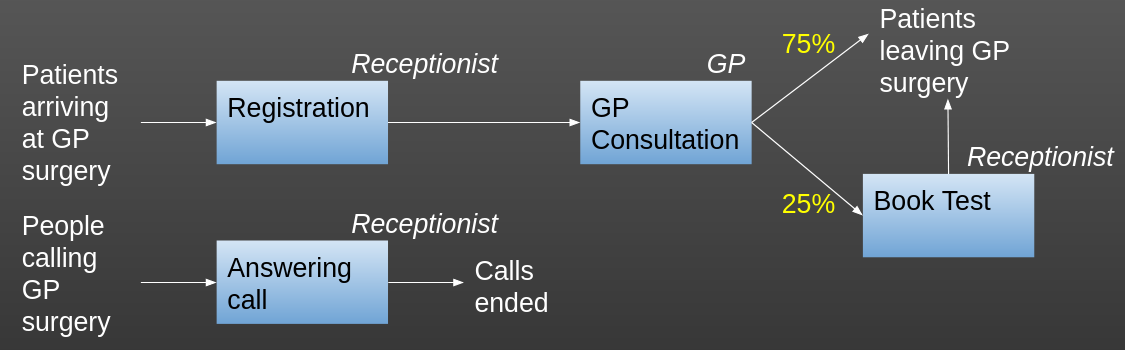
\includegraphics{images/exercise_gp.png}

Patients - arrive into the GP surgery around every 3 minutes - spend
around 2 minutes being registered - then spend around 8 minutes with the
GP.

Around a quarter of patients need to book a test at reception after
they've seen the GP, and this takes around 4 minutes.

In addition to registering patients and booking tests, receptionists
also answer incoming calls, which come in around every 10 minutes and
last about 4 minutes.

The surgery currently has 1 receptionist and 2 GPs. They feel there is a
problem in their system as they are receiving complaints about lengthy
delays both from patients and callers. They want you to build a
simulation model to find out what's happening and propose some
solutions.

Your model should represent a ``day in the life'' of the surgery, which
is open to both in-person patients and telephone callers for 8 hours
continuously.

Your trial should be at least 100 runs of the simulation.

\section{Required outputs}\label{required-outputs}

The surgery is only interested in queuing times for each of the queues
in the system (you don't need to worry about storing sampled activity
times for example), but they would like to look at the results for
patients and callers separately. You should give them mean results as a
minimum, but you may consider providing additional results too.

You also need to calculate and provide them with the mean queuing times
across the trial (eg mean queue for registration across all runs, for GP
etc - so four numbers that you would report). You'll need a new method
in your Trial class to calculate this. You should find this a helpful
output, as it'll help you compare scenarios easily. Report these means
to 1 decimal place.

\section{Goal}\label{goal}

Once you've built the model, use it to - a) identify where you think the
problem is - b) provide proposals for how you would fix it (this can
include anything you like - they are open to suggestions - more
resources, changes to processes to cut activity times, having the GP
book the test, anything you can think of!

Try different things, different solutions.

\begin{tcolorbox}[enhanced jigsaw, colframe=quarto-callout-tip-color-frame, bottomtitle=1mm, breakable, rightrule=.15mm, coltitle=black, colbacktitle=quarto-callout-tip-color!10!white, opacityback=0, leftrule=.75mm, arc=.35mm, toptitle=1mm, title=\textcolor{quarto-callout-tip-color}{\faLightbulb}\hspace{0.5em}{Tip}, titlerule=0mm, colback=white, toprule=.15mm, bottomrule=.15mm, left=2mm, opacitybacktitle=0.6]

Take a copy of the original working file for the base case scenario
first :)

\end{tcolorbox}

\part{Part 3 - Extending Your Model}

\chapter{Warm Up Periods}\label{sec-warmup}

In the models we've created so far patients start coming in when the
service opens, and then all leave when it closes.

But what if our system isn't like that? What if we have a system that is
never empty - like an Emergency Department?

By default, a DES model assumes that our system is empty at the start of
a simulation run. But if we were modelling an ED, that would skew (throw
off) our results, as the initial period during which patients were
coming in to an empty system wouldn't represent what's happening in the
real world - known as the \textbf{Initialisation Bias}.

The solution to this in DES modelling is to use a Warm Up Period.

The idea of a warm up period is simple. We run the model as normal -
from empty - but for a period of time (the warm up period) we don't
collect results.

The model continues to run as normal, it's just we don't count what's
happening.

\begin{tcolorbox}[enhanced jigsaw, colframe=quarto-callout-warning-color-frame, bottomtitle=1mm, breakable, rightrule=.15mm, coltitle=black, colbacktitle=quarto-callout-warning-color!10!white, opacityback=0, leftrule=.75mm, arc=.35mm, toptitle=1mm, title=\textcolor{quarto-callout-warning-color}{\faExclamationTriangle}\hspace{0.5em}{Warning}, titlerule=0mm, colback=white, toprule=.15mm, bottomrule=.15mm, left=2mm, opacitybacktitle=0.6]

If you don't use a warm-up period, you may find that the average waits
you give are a lot lower than the true state - the average will be
pulled lower by the earlier period of results before queues build up to
their normal levels.

\end{tcolorbox}

\section{How long should a warm-up period
be?}\label{how-long-should-a-warm-up-period-be}

The length of the warm up period is up to you as the modeller to define.

You could be very precise about analysing it and use statistical testing
to identify when the system reaches equilibrium (see
https://eudl.eu/pdf/10.4108/ICST.SIMUTOOLS2009.5603 as an example).

Or you could plot what's happening over time by eye and make an
estimate.

Or you could just set your warm up period long enough that it'll be
representative when it starts collecting results.

\section{Implementing the warm-up
period}\label{implementing-the-warm-up-period}

Implementing a warm up period in SimPy is really easy.

We just simply check the current time whenever we go to calculate /
store a result, and see if it's beyond the warm up period. If it is, we
do it. If it's not, we don't.

Let's look at an example. This is a slightly amended version of the
model of patients coming in for a nurse consultation with a few tweaks
(longer duration, more runs, added trial results calculation)

We're going to assume this is a system that's open 24 hours - let's
imagine this is a triage function at an emergency department.

I've marked the bits I've added to include warm up with \#\#NEW

\subsection{The g class}\label{the-g-class-2}

First we add in a new parameter - the length of the warm-up period.

Here, the sim duration has been set to 2880, and the warm-up-period to
half of this (1440). You don't need to stick to this pattern - your
warm-up could even be longer than your results collection if you want!

\phantomsection\label{g_class}
\begin{Shaded}
\begin{Highlighting}[]
\CommentTok{\# Class to store global parameter values.}
\KeywordTok{class}\NormalTok{ g:}
    \CommentTok{\# Inter{-}arrival times}
\NormalTok{    patient\_inter }\OperatorTok{=} \DecValTok{5}

    \CommentTok{\# Activity times}
\NormalTok{    mean\_n\_consult\_time }\OperatorTok{=} \DecValTok{6}

    \CommentTok{\# Resource numbers}
\NormalTok{    number\_of\_nurses }\OperatorTok{=} \DecValTok{1}

    \CommentTok{\# Simulation meta parameters}
\NormalTok{    sim\_duration }\OperatorTok{=} \DecValTok{2880}
\NormalTok{    warm\_up\_period }\OperatorTok{=} \DecValTok{1440} \CommentTok{\#\#NEW {-} this will be in addition to the sim\_duration}
\NormalTok{    number\_of\_runs }\OperatorTok{=} \DecValTok{100}
\end{Highlighting}
\end{Shaded}

\begin{tcolorbox}[enhanced jigsaw, colframe=quarto-callout-tip-color-frame, bottomtitle=1mm, breakable, rightrule=.15mm, coltitle=black, colbacktitle=quarto-callout-tip-color!10!white, opacityback=0, leftrule=.75mm, arc=.35mm, toptitle=1mm, title=\textcolor{quarto-callout-tip-color}{\faLightbulb}\hspace{0.5em}{Tip}, titlerule=0mm, colback=white, toprule=.15mm, bottomrule=.15mm, left=2mm, opacitybacktitle=0.6]

If you find it easier to keep track of, you could define your warm-up
like this instead.

\phantomsection\label{g_class_alt}
\begin{Shaded}
\begin{Highlighting}[]
\NormalTok{results\_collection\_period }\OperatorTok{=} \DecValTok{2880}
\NormalTok{warm\_up\_period }\OperatorTok{=} \DecValTok{1440}
\NormalTok{total\_sim\_duration }\OperatorTok{=}\NormalTok{ results\_collection\_period }\OperatorTok{+}\NormalTok{ warm\_up\_period}
\end{Highlighting}
\end{Shaded}

\end{tcolorbox}

\subsection{The patient class}\label{the-patient-class-2}

Our patient class is unchanged.

\subsection{The model class}\label{the-model-class-2}

In the model class, the `attend\_clinic' method changes.

We look at the current elapsed simulation time with the attribute
\texttt{self.env.now}

Then, whenever a patient attends the clinic and is using a nurse
resource, we check whether the current simulation time is later than the
number of time units we've set as our warm-up.

\subsubsection{The attend\_clinic
method}\label{the-attend_clinic-method-1}

\phantomsection\label{attend_clinic_func}
\begin{Shaded}
\begin{Highlighting}[]
\CommentTok{\# Generator function representing pathway for patients attending the}
\CommentTok{\# clinic.}
\KeywordTok{def}\NormalTok{ attend\_clinic(}\VariableTok{self}\NormalTok{, patient):}
    \CommentTok{\# Nurse consultation activity}
\NormalTok{    start\_q\_nurse }\OperatorTok{=} \VariableTok{self}\NormalTok{.env.now}

    \ControlFlowTok{with} \VariableTok{self}\NormalTok{.nurse.request() }\ImportTok{as}\NormalTok{ req:}
        \ControlFlowTok{yield}\NormalTok{ req}

\NormalTok{        end\_q\_nurse }\OperatorTok{=} \VariableTok{self}\NormalTok{.env.now}

\NormalTok{        patient.q\_time\_nurse }\OperatorTok{=}\NormalTok{ end\_q\_nurse }\OperatorTok{{-}}\NormalTok{ start\_q\_nurse}

        \CommentTok{\#\#NEW {-} this checks whether the warm up period has passed before}
        \CommentTok{\# adding any results}
        \ControlFlowTok{if} \VariableTok{self}\NormalTok{.env.now }\OperatorTok{\textgreater{}}\NormalTok{ g.warm\_up\_period:}
            \VariableTok{self}\NormalTok{.results\_df.at[patient.}\BuiltInTok{id}\NormalTok{, }\StringTok{"Q Time Nurse"}\NormalTok{] }\OperatorTok{=}\NormalTok{ (}
\NormalTok{                patient.q\_time\_nurse}
\NormalTok{            )}

\NormalTok{        sampled\_nurse\_act\_time }\OperatorTok{=}\NormalTok{ random.expovariate(}\FloatTok{1.0} \OperatorTok{/}
\NormalTok{                                                    g.mean\_n\_consult\_time)}

        \ControlFlowTok{yield} \VariableTok{self}\NormalTok{.env.timeout(sampled\_nurse\_act\_time)}
\end{Highlighting}
\end{Shaded}

For example, if the simulation time is at 840 and our warm\_up is 1440,
this bit of code - which adds the queuing time for this patient to our
records - won't run:

\phantomsection\label{warm_up_bypassed_code}
\begin{Shaded}
\begin{Highlighting}[]
\VariableTok{self}\NormalTok{.results\_df.at[patient.}\BuiltInTok{id}\NormalTok{, }\StringTok{"Q Time Nurse"}\NormalTok{] }\OperatorTok{=}\NormalTok{ (}
\NormalTok{    patient.q\_time\_nurse}
\NormalTok{)}
\end{Highlighting}
\end{Shaded}

However, if the simulation time is 1680, for example, it will.

\subsection{the calculate\_run\_results
method}\label{the-calculate_run_results-method-1}

As we now won't count the first patient, we need to remove the dummy
first patient result entry we created when we set up the dataframe.

\phantomsection\label{dummy_remove}
\begin{Shaded}
\begin{Highlighting}[]
\CommentTok{\# Method to calculate and store results over the run}
\KeywordTok{def}\NormalTok{ calculate\_run\_results(}\VariableTok{self}\NormalTok{):}
    \VariableTok{self}\NormalTok{.results\_df.drop([}\DecValTok{1}\NormalTok{], inplace}\OperatorTok{=}\VariableTok{True}\NormalTok{) }\CommentTok{\#\#NEW}

    \VariableTok{self}\NormalTok{.mean\_q\_time\_nurse }\OperatorTok{=} \VariableTok{self}\NormalTok{.results\_df[}\StringTok{"Q Time Nurse"}\NormalTok{].mean()}
\end{Highlighting}
\end{Shaded}

\subsubsection{The run method}\label{the-run-method-1}

Next we need to tweak the duration of our model to reflect the
combination of the period we want to collect results for and the warm-up
period.

\phantomsection\label{single_run}
\begin{Shaded}
\begin{Highlighting}[]
\CommentTok{\# Method to run a single run of the simulation}
\KeywordTok{def}\NormalTok{ run(}\VariableTok{self}\NormalTok{):}
    \CommentTok{\# Start up DES generators}
    \VariableTok{self}\NormalTok{.env.process(}\VariableTok{self}\NormalTok{.generator\_patient\_arrivals())}

    \CommentTok{\# Run for the duration specified in g class}
    \CommentTok{\#\#NEW {-} we need to tell the simulation to run for the specified duration}
    \CommentTok{\# + the warm up period if we still want the specified duration in full}
    \VariableTok{self}\NormalTok{.env.run(until}\OperatorTok{=}\NormalTok{(g.sim\_duration }\OperatorTok{+}\NormalTok{ g.warm\_up\_period))}

    \CommentTok{\# Calculate results over the run}
    \VariableTok{self}\NormalTok{.calculate\_run\_results()}

    \CommentTok{\# Print patient level results for this run}
    \BuiltInTok{print}\NormalTok{ (}\SpecialStringTok{f"Run Number }\SpecialCharTok{\{}\VariableTok{self}\SpecialCharTok{.}\NormalTok{run\_number}\SpecialCharTok{\}}\SpecialStringTok{"}\NormalTok{)}
    \BuiltInTok{print}\NormalTok{ (}\VariableTok{self}\NormalTok{.results\_df)}
\end{Highlighting}
\end{Shaded}

\subsection{The Trial class}\label{the-trial-class-2}

Our trial class is unchanged.

\section{The impact of the warm-up
period}\label{the-impact-of-the-warm-up-period}

Let's compare the results we get with and without the warm-up period.

\subsection{Editing our results
method}\label{editing-our-results-method}

To make it easier to look at the outputs, I'm going to modify two
methods slightly.

First, we modify the \texttt{run} method of the \texttt{Model} class
slightly to swap from print the patient level dataframes to returning
them as an output.

\begin{Shaded}
\begin{Highlighting}[]
\CommentTok{\# Method to run a single run of the simulation}
\KeywordTok{def}\NormalTok{ run(}\VariableTok{self}\NormalTok{):}
    \CommentTok{\# Start up DES generators}
    \VariableTok{self}\NormalTok{.env.process(}\VariableTok{self}\NormalTok{.generator\_patient\_arrivals())}

    \CommentTok{\# Run for the duration specified in g class}
    \CommentTok{\# We need to tell the simulation to run for the specified duration}
    \CommentTok{\# + the warm up period if we still want the specified duration in full}
    \VariableTok{self}\NormalTok{.env.run(until}\OperatorTok{=}\NormalTok{(g.sim\_duration }\OperatorTok{+}\NormalTok{ g.warm\_up\_period))}

    \CommentTok{\# Calculate results over the run}
    \VariableTok{self}\NormalTok{.calculate\_run\_results()}

    \CommentTok{\# Return patient level results for this run}
    \ControlFlowTok{return}\NormalTok{ (}\VariableTok{self}\NormalTok{.results\_df) }\CommentTok{\#\#NEW}
\end{Highlighting}
\end{Shaded}

Next, we modify the \texttt{run\_trial} method of the \texttt{Trial}
class so that we get multiple outputs: the full patient level
dataframes, a summary of results per trial, and an overall average
figure for all of the trials.

\phantomsection\label{edited_results_method}
\begin{Shaded}
\begin{Highlighting}[]
\CommentTok{\# Method to run a trial}
\KeywordTok{def}\NormalTok{ run\_trial(}\VariableTok{self}\NormalTok{):}
    \CommentTok{\# Run the simulation for the number of runs specified in g class.}
    \CommentTok{\# For each run, we create a new instance of the Model class and call its}
    \CommentTok{\# run method, which sets everything else in motion.  Once the run has}
    \CommentTok{\# completed, we grab out the stored run results and store it against}
    \CommentTok{\# the run number in the trial results dataframe. We also return the}
    \CommentTok{\# full patient{-}level dataframes.}

    \CommentTok{\# First, create an empty list for storing our patient{-}level dataframes.}
\NormalTok{    results\_dfs }\OperatorTok{=}\NormalTok{ []}

    \ControlFlowTok{for}\NormalTok{ run }\KeywordTok{in} \BuiltInTok{range}\NormalTok{(g.number\_of\_runs):}
\NormalTok{        my\_model }\OperatorTok{=}\NormalTok{ Model(run)}
\NormalTok{        patient\_level\_results }\OperatorTok{=}\NormalTok{ my\_model.run()}

        \BuiltInTok{print}\NormalTok{( }\VariableTok{self}\NormalTok{.df\_trial\_results)}
        \CommentTok{\# First let\textquotesingle{}s record our mean wait time for this run}
        \VariableTok{self}\NormalTok{.df\_trial\_results.loc[run] }\OperatorTok{=}\NormalTok{ [my\_model.mean\_q\_time\_nurse]}

        \CommentTok{\# Next let\textquotesingle{}s work on our patient{-}level results dataframes}
        \CommentTok{\# We start by rounding everything to 2 decimal places}
\NormalTok{        patient\_level\_results }\OperatorTok{=}\NormalTok{ patient\_level\_results.}\BuiltInTok{round}\NormalTok{(}\DecValTok{2}\NormalTok{)}
        \CommentTok{\# Add a new column recording the run}
\NormalTok{        patient\_level\_results[}\StringTok{\textquotesingle{}run\textquotesingle{}}\NormalTok{] }\OperatorTok{=}\NormalTok{ run}
        \CommentTok{\# Now we\textquotesingle{}re just going to add this to our empty list (or, after the first}
        \CommentTok{\# time we loop through, as an extra dataframe in our list)}
\NormalTok{        results\_dfs.append(patient\_level\_results)}

\NormalTok{    all\_results\_patient\_level }\OperatorTok{=}\NormalTok{ pd.concat(results\_dfs)}

    \CommentTok{\# This calculates the attribute self.mean\_q\_time\_nurse\_trial}
    \VariableTok{self}\NormalTok{.calculate\_means\_over\_trial()}

    \CommentTok{\# Once the trial (ie all runs) has completed, return the results}
    \ControlFlowTok{return} \VariableTok{self}\NormalTok{.df\_trial\_results, all\_results\_patient\_level, }\VariableTok{self}\NormalTok{.mean\_q\_time\_nurse\_trial}
\end{Highlighting}
\end{Shaded}

\subsection{The full updated code}\label{the-full-updated-code}

\phantomsection\label{code_full_warm_up}
\begin{Shaded}
\begin{Highlighting}[]
\ImportTok{import}\NormalTok{ simpy}
\ImportTok{import}\NormalTok{ random}
\ImportTok{import}\NormalTok{ pandas }\ImportTok{as}\NormalTok{ pd}

\CommentTok{\# Class to store global parameter values.}
\KeywordTok{class}\NormalTok{ g:}
    \CommentTok{\# Inter{-}arrival times}
\NormalTok{    patient\_inter }\OperatorTok{=} \DecValTok{5}

    \CommentTok{\# Activity times}
\NormalTok{    mean\_n\_consult\_time }\OperatorTok{=} \DecValTok{6}

    \CommentTok{\# Resource numbers}
\NormalTok{    number\_of\_nurses }\OperatorTok{=} \DecValTok{1}

    \CommentTok{\# Simulation meta parameters}
\NormalTok{    sim\_duration }\OperatorTok{=} \DecValTok{2880}
\NormalTok{    number\_of\_runs }\OperatorTok{=} \DecValTok{20}
\NormalTok{    warm\_up\_period }\OperatorTok{=} \DecValTok{1440} \CommentTok{\#\#NEW {-} this will be in addition to the sim\_duration}

\CommentTok{\# Class representing patients coming in to the clinic.}
\KeywordTok{class}\NormalTok{ Patient:}
    \KeywordTok{def} \FunctionTok{\_\_init\_\_}\NormalTok{(}\VariableTok{self}\NormalTok{, p\_id):}
        \VariableTok{self}\NormalTok{.}\BuiltInTok{id} \OperatorTok{=}\NormalTok{ p\_id}
        \VariableTok{self}\NormalTok{.q\_time\_nurse }\OperatorTok{=} \DecValTok{0}

\CommentTok{\# Class representing our model of the clinic.}
\KeywordTok{class}\NormalTok{ Model:}
    \CommentTok{\# Constructor}
    \KeywordTok{def} \FunctionTok{\_\_init\_\_}\NormalTok{(}\VariableTok{self}\NormalTok{, run\_number):}
        \CommentTok{\# Set up SimPy environment}
        \VariableTok{self}\NormalTok{.env }\OperatorTok{=}\NormalTok{ simpy.Environment()}

        \CommentTok{\# Set up counters to use as entity IDs}
        \VariableTok{self}\NormalTok{.patient\_counter }\OperatorTok{=} \DecValTok{0}

        \CommentTok{\# Set up resources}
        \VariableTok{self}\NormalTok{.nurse }\OperatorTok{=}\NormalTok{ simpy.Resource(}\VariableTok{self}\NormalTok{.env, capacity}\OperatorTok{=}\NormalTok{g.number\_of\_nurses)}

        \CommentTok{\# Set run number from value passed in}
        \VariableTok{self}\NormalTok{.run\_number }\OperatorTok{=}\NormalTok{ run\_number}

        \CommentTok{\# Set up DataFrame to store patient{-}level results}
        \VariableTok{self}\NormalTok{.results\_df }\OperatorTok{=}\NormalTok{ pd.DataFrame()}
        \VariableTok{self}\NormalTok{.results\_df[}\StringTok{"Patient ID"}\NormalTok{] }\OperatorTok{=}\NormalTok{ [}\DecValTok{1}\NormalTok{]}
        \VariableTok{self}\NormalTok{.results\_df[}\StringTok{"Q Time Nurse"}\NormalTok{] }\OperatorTok{=}\NormalTok{ [}\FloatTok{0.0}\NormalTok{]}
        \VariableTok{self}\NormalTok{.results\_df.set\_index(}\StringTok{"Patient ID"}\NormalTok{, inplace}\OperatorTok{=}\VariableTok{True}\NormalTok{)}

        \CommentTok{\# Set up attributes that will store mean queuing times across the run}
        \VariableTok{self}\NormalTok{.mean\_q\_time\_nurse }\OperatorTok{=} \DecValTok{0}

    \CommentTok{\# Generator function that represents the DES generator for patient arrivals}
    \KeywordTok{def}\NormalTok{ generator\_patient\_arrivals(}\VariableTok{self}\NormalTok{):}
        \ControlFlowTok{while} \VariableTok{True}\NormalTok{:}
            \VariableTok{self}\NormalTok{.patient\_counter }\OperatorTok{+=} \DecValTok{1}

\NormalTok{            p }\OperatorTok{=}\NormalTok{ Patient(}\VariableTok{self}\NormalTok{.patient\_counter)}

            \VariableTok{self}\NormalTok{.env.process(}\VariableTok{self}\NormalTok{.attend\_clinic(p))}

\NormalTok{            sampled\_inter }\OperatorTok{=}\NormalTok{ random.expovariate(}\FloatTok{1.0} \OperatorTok{/}\NormalTok{ g.patient\_inter)}

            \ControlFlowTok{yield} \VariableTok{self}\NormalTok{.env.timeout(sampled\_inter)}

    \CommentTok{\# Generator function representing pathway for patients attending the}
    \CommentTok{\# clinic.}
    \KeywordTok{def}\NormalTok{ attend\_clinic(}\VariableTok{self}\NormalTok{, patient):}
        \CommentTok{\# Nurse consultation activity}
\NormalTok{        start\_q\_nurse }\OperatorTok{=} \VariableTok{self}\NormalTok{.env.now}

        \ControlFlowTok{with} \VariableTok{self}\NormalTok{.nurse.request() }\ImportTok{as}\NormalTok{ req:}
            \ControlFlowTok{yield}\NormalTok{ req}

\NormalTok{            end\_q\_nurse }\OperatorTok{=} \VariableTok{self}\NormalTok{.env.now}

\NormalTok{            patient.q\_time\_nurse }\OperatorTok{=}\NormalTok{ end\_q\_nurse }\OperatorTok{{-}}\NormalTok{ start\_q\_nurse}

            \CommentTok{\#\#NEW {-} this checks whether the warm up period has passed before}
            \CommentTok{\# adding any results}
            \ControlFlowTok{if} \VariableTok{self}\NormalTok{.env.now }\OperatorTok{\textgreater{}}\NormalTok{ g.warm\_up\_period:}
                \VariableTok{self}\NormalTok{.results\_df.at[patient.}\BuiltInTok{id}\NormalTok{, }\StringTok{"Q Time Nurse"}\NormalTok{] }\OperatorTok{=}\NormalTok{ (}
\NormalTok{                    patient.q\_time\_nurse}
\NormalTok{                )}

\NormalTok{            sampled\_nurse\_act\_time }\OperatorTok{=}\NormalTok{ random.expovariate(}\FloatTok{1.0} \OperatorTok{/}
\NormalTok{                                                        g.mean\_n\_consult\_time)}

            \ControlFlowTok{yield} \VariableTok{self}\NormalTok{.env.timeout(sampled\_nurse\_act\_time)}

    \CommentTok{\# Method to calculate and store results over the run}
    \KeywordTok{def}\NormalTok{ calculate\_run\_results(}\VariableTok{self}\NormalTok{):}
        \CommentTok{\#\#NEW {-} as we now won\textquotesingle{}t count the first patient, we need to remove}
        \CommentTok{\# the dummy first patient result entry we created when we set up the}
        \CommentTok{\# dataframe}
        \VariableTok{self}\NormalTok{.results\_df.drop([}\DecValTok{1}\NormalTok{], inplace}\OperatorTok{=}\VariableTok{True}\NormalTok{)}

        \VariableTok{self}\NormalTok{.mean\_q\_time\_nurse }\OperatorTok{=} \VariableTok{self}\NormalTok{.results\_df[}\StringTok{"Q Time Nurse"}\NormalTok{].mean()}

    \CommentTok{\# Method to run a single run of the simulation}
    \KeywordTok{def}\NormalTok{ run(}\VariableTok{self}\NormalTok{):}
        \CommentTok{\# Start up DES generators}
        \VariableTok{self}\NormalTok{.env.process(}\VariableTok{self}\NormalTok{.generator\_patient\_arrivals())}

        \CommentTok{\# Run for the duration specified in g class}
        \CommentTok{\#\#NEW {-} we need to tell the simulation to run for the specified duration}
        \CommentTok{\# + the warm up period if we still want the specified duration in full}
        \VariableTok{self}\NormalTok{.env.run(until}\OperatorTok{=}\NormalTok{(g.sim\_duration }\OperatorTok{+}\NormalTok{ g.warm\_up\_period))}

        \CommentTok{\# Calculate results over the run}
        \VariableTok{self}\NormalTok{.calculate\_run\_results()}

        \CommentTok{\# Return patient level results for this run}
        \ControlFlowTok{return}\NormalTok{ (}\VariableTok{self}\NormalTok{.results\_df)}

\CommentTok{\# Class representing a Trial for our simulation}
\KeywordTok{class}\NormalTok{ Trial:}
    \CommentTok{\# Constructor}
    \KeywordTok{def}  \FunctionTok{\_\_init\_\_}\NormalTok{(}\VariableTok{self}\NormalTok{):}
        \VariableTok{self}\NormalTok{.df\_trial\_results }\OperatorTok{=}\NormalTok{ pd.DataFrame()}
        \VariableTok{self}\NormalTok{.df\_trial\_results[}\StringTok{"Run Number"}\NormalTok{] }\OperatorTok{=}\NormalTok{ [}\DecValTok{0}\NormalTok{]}
        \VariableTok{self}\NormalTok{.df\_trial\_results[}\StringTok{"Mean Q Time Nurse"}\NormalTok{] }\OperatorTok{=}\NormalTok{ [}\FloatTok{0.0}\NormalTok{]}
        \VariableTok{self}\NormalTok{.df\_trial\_results.set\_index(}\StringTok{"Run Number"}\NormalTok{, inplace}\OperatorTok{=}\VariableTok{True}\NormalTok{)}

    \CommentTok{\# Method to calculate and store means across runs in the trial}
    \KeywordTok{def}\NormalTok{ calculate\_means\_over\_trial(}\VariableTok{self}\NormalTok{):}
        \VariableTok{self}\NormalTok{.mean\_q\_time\_nurse\_trial }\OperatorTok{=}\NormalTok{ (}
            \VariableTok{self}\NormalTok{.df\_trial\_results[}\StringTok{"Mean Q Time Nurse"}\NormalTok{].mean()}
\NormalTok{        )}

    \KeywordTok{def}\NormalTok{ run\_trial(}\VariableTok{self}\NormalTok{):}
        \CommentTok{\# Run the simulation for the number of runs specified in g class.}
        \CommentTok{\# For each run, we create a new instance of the Model class and call its}
        \CommentTok{\# run method, which sets everything else in motion.  Once the run has}
        \CommentTok{\# completed, we grab out the stored run results and store it against}
        \CommentTok{\# the run number in the trial results dataframe. We also return the}
        \CommentTok{\# full patient{-}level dataframes.}

        \CommentTok{\# First, create an empty list for storing our patient{-}level dataframes.}
\NormalTok{        results\_dfs }\OperatorTok{=}\NormalTok{ []}

        \ControlFlowTok{for}\NormalTok{ run }\KeywordTok{in} \BuiltInTok{range}\NormalTok{(g.number\_of\_runs):}
\NormalTok{            my\_model }\OperatorTok{=}\NormalTok{ Model(run)}
\NormalTok{            patient\_level\_results }\OperatorTok{=}\NormalTok{ my\_model.run()}

            \BuiltInTok{print}\NormalTok{( }\VariableTok{self}\NormalTok{.df\_trial\_results)}
            \CommentTok{\# First let\textquotesingle{}s record our mean wait time for this run}
            \VariableTok{self}\NormalTok{.df\_trial\_results.loc[run] }\OperatorTok{=}\NormalTok{ [my\_model.mean\_q\_time\_nurse]}

            \CommentTok{\# Next let\textquotesingle{}s work on our patient{-}level results dataframes}
            \CommentTok{\# We start by rounding everything to 2 decimal places}
\NormalTok{            patient\_level\_results }\OperatorTok{=}\NormalTok{ patient\_level\_results.}\BuiltInTok{round}\NormalTok{(}\DecValTok{2}\NormalTok{)}
            \CommentTok{\# Add a new column recording the run}
\NormalTok{            patient\_level\_results[}\StringTok{\textquotesingle{}run\textquotesingle{}}\NormalTok{] }\OperatorTok{=}\NormalTok{ run}
            \CommentTok{\# Now we\textquotesingle{}re just going to add this to our empty list (or, after the first}
            \CommentTok{\# time we loop through, as an extra dataframe in our list)}
\NormalTok{            results\_dfs.append(patient\_level\_results)}

\NormalTok{        all\_results\_patient\_level }\OperatorTok{=}\NormalTok{ pd.concat(results\_dfs)}

        \CommentTok{\# This calculates the attribute self.mean\_q\_time\_nurse\_trial}
        \VariableTok{self}\NormalTok{.calculate\_means\_over\_trial()}

        \CommentTok{\# Once the trial (ie all runs) has completed, return the results}
        \ControlFlowTok{return} \VariableTok{self}\NormalTok{.df\_trial\_results, all\_results\_patient\_level, }\VariableTok{self}\NormalTok{.mean\_q\_time\_nurse\_trial}

    \CommentTok{\# Method to print trial results, including averages across runs}
    \KeywordTok{def}\NormalTok{ print\_trial\_results(}\VariableTok{self}\NormalTok{):}
        \BuiltInTok{print}\NormalTok{ (}\StringTok{"Trial Results"}\NormalTok{)}
        \CommentTok{\# EDIT: We are omitting the printouts of the patient level data for now}
        \CommentTok{\# print (self.df\_trial\_results)}

        \BuiltInTok{print}\NormalTok{ (}\SpecialStringTok{f"Mean Q Nurse : }\SpecialCharTok{\{}\VariableTok{self}\SpecialCharTok{.}\NormalTok{mean\_q\_time\_nurse\_trial}\SpecialCharTok{:.1f\}}\SpecialStringTok{ minutes"}\NormalTok{)}

\CommentTok{\# Create new instance of Trial and run it}
\NormalTok{my\_trial }\OperatorTok{=}\NormalTok{ Trial()}
\NormalTok{df\_trial\_results\_warmup, all\_results\_patient\_level\_warmup, means\_over\_trial\_warmup }\OperatorTok{=}\NormalTok{ my\_trial.run\_trial()}
\end{Highlighting}
\end{Shaded}

\begin{verbatim}
            Mean Q Time Nurse
Run Number                   
0                         0.0
            Mean Q Time Nurse
Run Number                   
0                  493.372377
            Mean Q Time Nurse
Run Number                   
0                  493.372377
1                  557.079172
            Mean Q Time Nurse
Run Number                   
0                  493.372377
1                  557.079172
2                  365.711031
            Mean Q Time Nurse
Run Number                   
0                  493.372377
1                  557.079172
2                  365.711031
3                  635.010703
            Mean Q Time Nurse
Run Number                   
0                  493.372377
1                  557.079172
2                  365.711031
3                  635.010703
4                  355.538018
            Mean Q Time Nurse
Run Number                   
0                  493.372377
1                  557.079172
2                  365.711031
3                  635.010703
4                  355.538018
5                  493.917168
            Mean Q Time Nurse
Run Number                   
0                  493.372377
1                  557.079172
2                  365.711031
3                  635.010703
4                  355.538018
5                  493.917168
6                  524.191600
            Mean Q Time Nurse
Run Number                   
0                  493.372377
1                  557.079172
2                  365.711031
3                  635.010703
4                  355.538018
5                  493.917168
6                  524.191600
7                  389.265176
            Mean Q Time Nurse
Run Number                   
0                  493.372377
1                  557.079172
2                  365.711031
3                  635.010703
4                  355.538018
5                  493.917168
6                  524.191600
7                  389.265176
8                  675.832703
            Mean Q Time Nurse
Run Number                   
0                  493.372377
1                  557.079172
2                  365.711031
3                  635.010703
4                  355.538018
5                  493.917168
6                  524.191600
7                  389.265176
8                  675.832703
9                  622.088894
            Mean Q Time Nurse
Run Number                   
0                  493.372377
1                  557.079172
2                  365.711031
3                  635.010703
4                  355.538018
5                  493.917168
6                  524.191600
7                  389.265176
8                  675.832703
9                  622.088894
10                 570.369036
            Mean Q Time Nurse
Run Number                   
0                  493.372377
1                  557.079172
2                  365.711031
3                  635.010703
4                  355.538018
5                  493.917168
6                  524.191600
7                  389.265176
8                  675.832703
9                  622.088894
10                 570.369036
11                 321.953674
            Mean Q Time Nurse
Run Number                   
0                  493.372377
1                  557.079172
2                  365.711031
3                  635.010703
4                  355.538018
5                  493.917168
6                  524.191600
7                  389.265176
8                  675.832703
9                  622.088894
10                 570.369036
11                 321.953674
12                 428.473207
            Mean Q Time Nurse
Run Number                   
0                  493.372377
1                  557.079172
2                  365.711031
3                  635.010703
4                  355.538018
5                  493.917168
6                  524.191600
7                  389.265176
8                  675.832703
9                  622.088894
10                 570.369036
11                 321.953674
12                 428.473207
13                 803.520537
            Mean Q Time Nurse
Run Number                   
0                  493.372377
1                  557.079172
2                  365.711031
3                  635.010703
4                  355.538018
5                  493.917168
6                  524.191600
7                  389.265176
8                  675.832703
9                  622.088894
10                 570.369036
11                 321.953674
12                 428.473207
13                 803.520537
14                 290.876555
            Mean Q Time Nurse
Run Number                   
0                  493.372377
1                  557.079172
2                  365.711031
3                  635.010703
4                  355.538018
5                  493.917168
6                  524.191600
7                  389.265176
8                  675.832703
9                  622.088894
10                 570.369036
11                 321.953674
12                 428.473207
13                 803.520537
14                 290.876555
15                 500.755547
            Mean Q Time Nurse
Run Number                   
0                  493.372377
1                  557.079172
2                  365.711031
3                  635.010703
4                  355.538018
5                  493.917168
6                  524.191600
7                  389.265176
8                  675.832703
9                  622.088894
10                 570.369036
11                 321.953674
12                 428.473207
13                 803.520537
14                 290.876555
15                 500.755547
16                 690.680715
            Mean Q Time Nurse
Run Number                   
0                  493.372377
1                  557.079172
2                  365.711031
3                  635.010703
4                  355.538018
5                  493.917168
6                  524.191600
7                  389.265176
8                  675.832703
9                  622.088894
10                 570.369036
11                 321.953674
12                 428.473207
13                 803.520537
14                 290.876555
15                 500.755547
16                 690.680715
17                 388.898637
            Mean Q Time Nurse
Run Number                   
0                  493.372377
1                  557.079172
2                  365.711031
3                  635.010703
4                  355.538018
5                  493.917168
6                  524.191600
7                  389.265176
8                  675.832703
9                  622.088894
10                 570.369036
11                 321.953674
12                 428.473207
13                 803.520537
14                 290.876555
15                 500.755547
16                 690.680715
17                 388.898637
18                 381.227734
\end{verbatim}

\phantomsection\label{code_full_no_warm_up}
\begin{verbatim}
            Mean Q Time Nurse
Run Number                   
0                         0.0
            Mean Q Time Nurse
Run Number                   
0                  288.880551
            Mean Q Time Nurse
Run Number                   
0                  288.880551
1                  490.223877
            Mean Q Time Nurse
Run Number                   
0                  288.880551
1                  490.223877
2                  198.260679
            Mean Q Time Nurse
Run Number                   
0                  288.880551
1                  490.223877
2                  198.260679
3                  238.286518
            Mean Q Time Nurse
Run Number                   
0                  288.880551
1                  490.223877
2                  198.260679
3                  238.286518
4                  299.336403
            Mean Q Time Nurse
Run Number                   
0                  288.880551
1                  490.223877
2                  198.260679
3                  238.286518
4                  299.336403
5                  354.808532
            Mean Q Time Nurse
Run Number                   
0                  288.880551
1                  490.223877
2                  198.260679
3                  238.286518
4                  299.336403
5                  354.808532
6                  412.313993
            Mean Q Time Nurse
Run Number                   
0                  288.880551
1                  490.223877
2                  198.260679
3                  238.286518
4                  299.336403
5                  354.808532
6                  412.313993
7                  392.528479
            Mean Q Time Nurse
Run Number                   
0                  288.880551
1                  490.223877
2                  198.260679
3                  238.286518
4                  299.336403
5                  354.808532
6                  412.313993
7                  392.528479
8                  260.694210
            Mean Q Time Nurse
Run Number                   
0                  288.880551
1                  490.223877
2                  198.260679
3                  238.286518
4                  299.336403
5                  354.808532
6                  412.313993
7                  392.528479
8                  260.694210
9                  521.748126
            Mean Q Time Nurse
Run Number                   
0                  288.880551
1                  490.223877
2                  198.260679
3                  238.286518
4                  299.336403
5                  354.808532
6                  412.313993
7                  392.528479
8                  260.694210
9                  521.748126
10                 304.188013
            Mean Q Time Nurse
Run Number                   
0                  288.880551
1                  490.223877
2                  198.260679
3                  238.286518
4                  299.336403
5                  354.808532
6                  412.313993
7                  392.528479
8                  260.694210
9                  521.748126
10                 304.188013
11                 315.551064
            Mean Q Time Nurse
Run Number                   
0                  288.880551
1                  490.223877
2                  198.260679
3                  238.286518
4                  299.336403
5                  354.808532
6                  412.313993
7                  392.528479
8                  260.694210
9                  521.748126
10                 304.188013
11                 315.551064
12                 318.929589
            Mean Q Time Nurse
Run Number                   
0                  288.880551
1                  490.223877
2                  198.260679
3                  238.286518
4                  299.336403
5                  354.808532
6                  412.313993
7                  392.528479
8                  260.694210
9                  521.748126
10                 304.188013
11                 315.551064
12                 318.929589
13                 351.904971
            Mean Q Time Nurse
Run Number                   
0                  288.880551
1                  490.223877
2                  198.260679
3                  238.286518
4                  299.336403
5                  354.808532
6                  412.313993
7                  392.528479
8                  260.694210
9                  521.748126
10                 304.188013
11                 315.551064
12                 318.929589
13                 351.904971
14                 346.586831
            Mean Q Time Nurse
Run Number                   
0                  288.880551
1                  490.223877
2                  198.260679
3                  238.286518
4                  299.336403
5                  354.808532
6                  412.313993
7                  392.528479
8                  260.694210
9                  521.748126
10                 304.188013
11                 315.551064
12                 318.929589
13                 351.904971
14                 346.586831
15                 321.439654
            Mean Q Time Nurse
Run Number                   
0                  288.880551
1                  490.223877
2                  198.260679
3                  238.286518
4                  299.336403
5                  354.808532
6                  412.313993
7                  392.528479
8                  260.694210
9                  521.748126
10                 304.188013
11                 315.551064
12                 318.929589
13                 351.904971
14                 346.586831
15                 321.439654
16                 354.412420
            Mean Q Time Nurse
Run Number                   
0                  288.880551
1                  490.223877
2                  198.260679
3                  238.286518
4                  299.336403
5                  354.808532
6                  412.313993
7                  392.528479
8                  260.694210
9                  521.748126
10                 304.188013
11                 315.551064
12                 318.929589
13                 351.904971
14                 346.586831
15                 321.439654
16                 354.412420
17                 374.551621
            Mean Q Time Nurse
Run Number                   
0                  288.880551
1                  490.223877
2                  198.260679
3                  238.286518
4                  299.336403
5                  354.808532
6                  412.313993
7                  392.528479
8                  260.694210
9                  521.748126
10                 304.188013
11                 315.551064
12                 318.929589
13                 351.904971
14                 346.586831
15                 321.439654
16                 354.412420
17                 374.551621
18                 476.553538
\end{verbatim}

\subsection{Comparing the results}\label{comparing-the-results}

\subsubsection{Patient-level dataframes}\label{patient-level-dataframes}

First, let's look at the first five rows of our patient dataframes.

Without the warm-up, our patient IDs start at 1.

\paragraph{Without warm-up}\label{without-warm-up}

\begin{Shaded}
\begin{Highlighting}[]
\NormalTok{all\_results\_patient\_level.head()}
\end{Highlighting}
\end{Shaded}

\phantomsection\label{results_p_level_head}
\begin{longtable}[]{@{}llll@{}}
\toprule\noalign{}
& Q Time Nurse & Time with Nurse & run \\
Patient ID & & & \\
\midrule\noalign{}
\endhead
\bottomrule\noalign{}
\endlastfoot
1 & 0.00 & 11.23 & 0 \\
2 & 4.49 & 3.55 & 0 \\
3 & 6.85 & 1.83 & 0 \\
4 & 0.00 & 16.44 & 0 \\
5 & 1.52 & 5.85 & 0 \\
\end{longtable}

\paragraph{With warm-up}\label{with-warm-up}

With the warm-up, our patient IDs start later.

\begin{Shaded}
\begin{Highlighting}[]
\NormalTok{all\_results\_patient\_level\_warmup.head()}
\end{Highlighting}
\end{Shaded}

\phantomsection\label{results_warmup_p_level_head}
\begin{longtable}[]{@{}lll@{}}
\toprule\noalign{}
& Q Time Nurse & run \\
Patient ID & & \\
\midrule\noalign{}
\endhead
\bottomrule\noalign{}
\endlastfoot
256 & 174.50 & 0 \\
257 & 174.53 & 0 \\
258 & 168.24 & 0 \\
259 & 165.03 & 0 \\
260 & 165.43 & 0 \\
\end{longtable}

\subsubsection{Per-run results}\label{per-run-results}

\paragraph{Without warm-up}\label{without-warm-up-1}

\begin{Shaded}
\begin{Highlighting}[]
\NormalTok{df\_trial\_results.}\BuiltInTok{round}\NormalTok{(}\DecValTok{2}\NormalTok{).head()}
\end{Highlighting}
\end{Shaded}

\phantomsection\label{results_trial_level_head}
\begin{longtable}[]{@{}ll@{}}
\toprule\noalign{}
& Mean Q Time Nurse \\
Run Number & \\
\midrule\noalign{}
\endhead
\bottomrule\noalign{}
\endlastfoot
0 & 288.88 \\
1 & 490.22 \\
2 & 198.26 \\
3 & 238.29 \\
4 & 299.34 \\
\end{longtable}

\paragraph{With warm-up}\label{with-warm-up-1}

With the warm-up, our patient IDs start later.

\begin{Shaded}
\begin{Highlighting}[]
\NormalTok{df\_trial\_results\_warmup.}\BuiltInTok{round}\NormalTok{(}\DecValTok{2}\NormalTok{).head()}
\end{Highlighting}
\end{Shaded}

\phantomsection\label{results_warmup_trial_level_head}
\begin{longtable}[]{@{}ll@{}}
\toprule\noalign{}
& Mean Q Time Nurse \\
Run Number & \\
\midrule\noalign{}
\endhead
\bottomrule\noalign{}
\endlastfoot
0 & 493.37 \\
1 & 557.08 \\
2 & 365.71 \\
3 & 635.01 \\
4 & 355.54 \\
\end{longtable}

\subsubsection{Overall results}\label{overall-results}

Without the warm up, our overall average wait time is

\begin{verbatim}
'358.6 minutes'
\end{verbatim}

With the warm up, our overall average wait time is

\begin{verbatim}
'482.39 minutes'
\end{verbatim}

You can see overall that the warm-up time can have a very significant
impact on our waiting times!

Let's look at this in a graph.

\subsubsection{Results over time}\label{results-over-time}

\begin{Shaded}
\begin{Highlighting}[]
\ImportTok{import}\NormalTok{ plotly.express }\ImportTok{as}\NormalTok{ px}

\NormalTok{df\_trial\_results }\OperatorTok{=}\NormalTok{ df\_trial\_results.reset\_index()}
\NormalTok{df\_trial\_results[}\StringTok{\textquotesingle{}Warm Up\textquotesingle{}}\NormalTok{] }\OperatorTok{=} \StringTok{\textquotesingle{}No Warm Up\textquotesingle{}}

\NormalTok{df\_trial\_results\_warmup }\OperatorTok{=}\NormalTok{ df\_trial\_results\_warmup.reset\_index()}
\NormalTok{df\_trial\_results\_warmup[}\StringTok{\textquotesingle{}Warm Up\textquotesingle{}}\NormalTok{] }\OperatorTok{=} \StringTok{\textquotesingle{}With Warm Up\textquotesingle{}}

\NormalTok{fig }\OperatorTok{=}\NormalTok{ px.histogram(}
\NormalTok{    pd.concat([df\_trial\_results, df\_trial\_results\_warmup]).}\BuiltInTok{round}\NormalTok{(}\DecValTok{2}\NormalTok{).reset\_index(),}
\NormalTok{    x}\OperatorTok{=}\StringTok{"Warm Up"}\NormalTok{,}
\NormalTok{    color}\OperatorTok{=}\StringTok{"Run Number"}\NormalTok{, y}\OperatorTok{=}\StringTok{"Mean Q Time Nurse"}\NormalTok{,}
\NormalTok{    barmode}\OperatorTok{=}\StringTok{\textquotesingle{}group\textquotesingle{}}\NormalTok{,}
\NormalTok{    title}\OperatorTok{=}\StringTok{\textquotesingle{}Average Queue Times per Run {-} With and Without Warmups\textquotesingle{}}\NormalTok{)}

\NormalTok{fig.show()}
\end{Highlighting}
\end{Shaded}

\begin{verbatim}
Unable to display output for mime type(s): text/html
\end{verbatim}

\begin{verbatim}
Unable to display output for mime type(s): application/vnd.plotly.v1+json, text/html
\end{verbatim}

\chapter{Priority-Based Queueing}\label{priority-based-queueing}

So far, we've assumed that the queues in our models follow a FIFO (First
in First Out) policy. This means that whoever has been queuing the
longest is seen next.

But in healthcare systems, very often there is an element of
prioritisation in a real world queue. Typically this represents the
severity of the patient's condition.

We can build in priority-based queuing in our SimPy models in a few
different ways - but one of the easiest is using something known as a
\textbf{PriorityResource}.

A PriorityResource is a class in SimPy that's like the standard Resource
class we've used so far, but also has functionality that allows it to
select which entity to pull out of a queue next based on a priority
value we specify.

The way this works in SimPy is :

\begin{enumerate}
\def\labelenumi{\arabic{enumi}.}
\item
  We set up resources that will be dealing with priority-based queues as
  PriorityResources rather than Resources
\item
  We have an attribute stored against the entity that specifies that
  entity's priority (with lower values indicating higher priority)
\item
  When we request a PriorityResource, we tell it the attribute to use to
  determine priority in that queue (this also means we could have
  multiple attributes for priority and use different ones for different
  queues).
\end{enumerate}

\section{Implementing priority-based
queueing}\label{implementing-priority-based-queueing}

\subsection{g class}\label{g-class-2}

The g class is unchanged

\subsection{Patient class}\label{patient-class}

Here we add an attribute of the patient that determines their priority
:::\{.callout-tip\} When using a priority resource

Lower value = higher priority :::

In this example, we just randomly pick a value between 1 and 5, but you
can use whatever logic you like.

In reality, you'd likely have probabilities to determine what priority a
patient is based on your data - maybe there's a 20\% chance they are a
high priority and an 80\% chance they are a low priority.

\begin{Shaded}
\begin{Highlighting}[]
\KeywordTok{class}\NormalTok{ Patient:}
    \KeywordTok{def} \FunctionTok{\_\_init\_\_}\NormalTok{(}\VariableTok{self}\NormalTok{, p\_id):}
        \VariableTok{self}\NormalTok{.}\BuiltInTok{id} \OperatorTok{=}\NormalTok{ p\_id}
        \VariableTok{self}\NormalTok{.q\_time\_nurse }\OperatorTok{=} \DecValTok{0}
        \CommentTok{\#\#NEW}
        \VariableTok{self}\NormalTok{.priority }\OperatorTok{=}\NormalTok{ random.randint(}\DecValTok{1}\NormalTok{,}\DecValTok{5}\NormalTok{)}
\end{Highlighting}
\end{Shaded}

\subsection{Model class}\label{model-class-2}

\subsubsection{\_init}\label{init}

Here we set up the nurse as an instance of PriorityResource rather than
Resource

\begin{Shaded}
\begin{Highlighting}[]
\KeywordTok{def} \FunctionTok{\_\_init\_\_}\NormalTok{(}\VariableTok{self}\NormalTok{, run\_number):}
        \CommentTok{\# Set up SimPy environment}
        \VariableTok{self}\NormalTok{.env }\OperatorTok{=}\NormalTok{ simpy.Environment()}

        \CommentTok{\# Set up counters to use as entity IDs}
        \VariableTok{self}\NormalTok{.patient\_counter }\OperatorTok{=} \DecValTok{0}

        \CommentTok{\# Set up resources}
        \CommentTok{\#\#NEW}
        \VariableTok{self}\NormalTok{.nurse }\OperatorTok{=}\NormalTok{ simpy.PriorityResource(}\VariableTok{self}\NormalTok{.env,}
\NormalTok{                                            capacity}\OperatorTok{=}\NormalTok{g.number\_of\_nurses)}

        \CommentTok{\# Set run number from value passed in}
        \VariableTok{self}\NormalTok{.run\_number }\OperatorTok{=}\NormalTok{ run\_number}


        \CommentTok{\# Set up DataFrame to store patient{-}level results}
        \VariableTok{self}\NormalTok{.results\_df }\OperatorTok{=}\NormalTok{ pd.DataFrame()}
        \VariableTok{self}\NormalTok{.results\_df[}\StringTok{"Patient ID"}\NormalTok{] }\OperatorTok{=}\NormalTok{ [}\DecValTok{1}\NormalTok{]}
        \VariableTok{self}\NormalTok{.results\_df[}\StringTok{"Q Time Nurse"}\NormalTok{] }\OperatorTok{=}\NormalTok{ [}\FloatTok{0.0}\NormalTok{]}
        \VariableTok{self}\NormalTok{.results\_df[}\StringTok{"Priority"}\NormalTok{] }\OperatorTok{=}\NormalTok{ [}\DecValTok{1}\NormalTok{] }\CommentTok{\#\#NEW}
        \VariableTok{self}\NormalTok{.results\_df.set\_index(}\StringTok{"Patient ID"}\NormalTok{, inplace}\OperatorTok{=}\VariableTok{True}\NormalTok{)}

        \CommentTok{\# Set up attributes that will store mean queuing times across the run}
        \VariableTok{self}\NormalTok{.mean\_q\_time\_nurse }\OperatorTok{=} \DecValTok{0}
\end{Highlighting}
\end{Shaded}

\subsubsection{attend\_clinic}\label{attend_clinic}

Near the beginning of the attend\_clinic() method, we have added a print
message so we can see how priority works.

\begin{tcolorbox}[enhanced jigsaw, colframe=quarto-callout-tip-color-frame, bottomtitle=1mm, breakable, rightrule=.15mm, coltitle=black, colbacktitle=quarto-callout-tip-color!10!white, opacityback=0, leftrule=.75mm, arc=.35mm, toptitle=1mm, title=\textcolor{quarto-callout-tip-color}{\faLightbulb}\hspace{0.5em}{Tip}, titlerule=0mm, colback=white, toprule=.15mm, bottomrule=.15mm, left=2mm, opacitybacktitle=0.6]

Logging in this way can help you check that your model is behaving as
expected.

\end{tcolorbox}

Now that the nurse is set up as a PriorityResource, we can pass in the
value that we want it to look at to determine who's seen next when we
request the resource (here, that's the priority attribute of the patient
we set up in the Patient class).

We have also added a step that records the patient priority to our
dataframe of individual patient results.

\begin{Shaded}
\begin{Highlighting}[]
\CommentTok{\# Generator function representing pathway for patients attending the}
    \CommentTok{\# clinic.}
    \KeywordTok{def}\NormalTok{ attend\_clinic(}\VariableTok{self}\NormalTok{, patient):}
        \CommentTok{\# Nurse consultation activity}
\NormalTok{        start\_q\_nurse }\OperatorTok{=} \VariableTok{self}\NormalTok{.env.now}

        \CommentTok{\#\#NEW}
        \BuiltInTok{print}\NormalTok{ (}\SpecialStringTok{f"Patient }\SpecialCharTok{\{}\NormalTok{patient}\SpecialCharTok{.}\BuiltInTok{id}\SpecialCharTok{\}}\SpecialStringTok{ with priority }\SpecialCharTok{\{}\NormalTok{patient}\SpecialCharTok{.}\NormalTok{priority}\SpecialCharTok{\}}\SpecialStringTok{ is"}\NormalTok{,}
               \StringTok{"queuing for the nurse."}\NormalTok{)}

        \CommentTok{\#\#NEW}
        \ControlFlowTok{with} \VariableTok{self}\NormalTok{.nurse.request(priority}\OperatorTok{=}\NormalTok{patient.priority) }\ImportTok{as}\NormalTok{ req:}
            \ControlFlowTok{yield}\NormalTok{ req}

\NormalTok{            end\_q\_nurse }\OperatorTok{=} \VariableTok{self}\NormalTok{.env.now}

            \CommentTok{\#\#NEW}
            \BuiltInTok{print}\NormalTok{ (}\SpecialStringTok{f"Patient }\SpecialCharTok{\{}\NormalTok{patient}\SpecialCharTok{.}\BuiltInTok{id}\SpecialCharTok{\}}\SpecialStringTok{ with priority }\SpecialCharTok{\{}\NormalTok{patient}\SpecialCharTok{.}\NormalTok{priority}\SpecialCharTok{\}}\SpecialStringTok{ is"}\NormalTok{,}
                   \SpecialStringTok{f"being seen at minute }\SpecialCharTok{\{}\VariableTok{self}\SpecialCharTok{.}\NormalTok{env}\SpecialCharTok{.}\NormalTok{now}\SpecialCharTok{\}}\SpecialStringTok{."}\NormalTok{)}

\NormalTok{            patient.q\_time\_nurse }\OperatorTok{=}\NormalTok{ end\_q\_nurse }\OperatorTok{{-}}\NormalTok{ start\_q\_nurse}

            \ControlFlowTok{if} \VariableTok{self}\NormalTok{.env.now }\OperatorTok{\textgreater{}}\NormalTok{ g.warm\_up\_period:}
                \VariableTok{self}\NormalTok{.results\_df.at[patient.}\BuiltInTok{id}\NormalTok{, }\StringTok{"Q Time Nurse"}\NormalTok{] }\OperatorTok{=}\NormalTok{ (}
\NormalTok{                    patient.q\_time\_nurse}
\NormalTok{                )}

                \CommentTok{\#\#NEW}
                \VariableTok{self}\NormalTok{.results\_df.at[patient.}\BuiltInTok{id}\NormalTok{, }\StringTok{"Priority"}\NormalTok{] }\OperatorTok{=}\NormalTok{ (}
\NormalTok{                    patient.priority}
\NormalTok{                )}

\NormalTok{            sampled\_nurse\_act\_time }\OperatorTok{=}\NormalTok{ random.expovariate(}\FloatTok{1.0} \OperatorTok{/}
\NormalTok{                                                        g.mean\_n\_consult\_time)}

            \ControlFlowTok{yield} \VariableTok{self}\NormalTok{.env.timeout(sampled\_nurse\_act\_time)}
\end{Highlighting}
\end{Shaded}

\subsection{Trial class}\label{trial-class-2}

The trial class is unchanged.

\section{The full code}\label{the-full-code}

The full code is given below.

\begin{tcolorbox}[enhanced jigsaw, colframe=quarto-callout-note-color-frame, bottomtitle=1mm, breakable, rightrule=.15mm, coltitle=black, colbacktitle=quarto-callout-note-color!10!white, opacityback=0, leftrule=.75mm, arc=.35mm, toptitle=1mm, title=\textcolor{quarto-callout-note-color}{\faInfo}\hspace{0.5em}{Click here to view the full code}, titlerule=0mm, colback=white, toprule=.15mm, bottomrule=.15mm, left=2mm, opacitybacktitle=0.6]

\begin{Shaded}
\begin{Highlighting}[]
\ImportTok{import}\NormalTok{ simpy}
\ImportTok{import}\NormalTok{ random}
\ImportTok{import}\NormalTok{ pandas }\ImportTok{as}\NormalTok{ pd}

\CommentTok{\# Class to store global parameter values.}
\KeywordTok{class}\NormalTok{ g:}
    \CommentTok{\# Inter{-}arrival times}
\NormalTok{    patient\_inter }\OperatorTok{=} \DecValTok{5}

    \CommentTok{\# Activity times}
\NormalTok{    mean\_n\_consult\_time }\OperatorTok{=} \DecValTok{6}

    \CommentTok{\# Resource numbers}
\NormalTok{    number\_of\_nurses }\OperatorTok{=} \DecValTok{1}

    \CommentTok{\#\#NEW {-} We\textquotesingle{}ve changed the parameters to have no warm{-}up}
    \CommentTok{\# Simulation meta parameters}
\NormalTok{    sim\_duration }\OperatorTok{=} \DecValTok{5000}
\NormalTok{    number\_of\_runs }\OperatorTok{=} \DecValTok{1}
\NormalTok{    warm\_up\_period }\OperatorTok{=} \DecValTok{0}

\CommentTok{\# Class representing patients coming in to the clinic.}
\KeywordTok{class}\NormalTok{ Patient:}
    \KeywordTok{def} \FunctionTok{\_\_init\_\_}\NormalTok{(}\VariableTok{self}\NormalTok{, p\_id):}
        \VariableTok{self}\NormalTok{.}\BuiltInTok{id} \OperatorTok{=}\NormalTok{ p\_id}
        \VariableTok{self}\NormalTok{.q\_time\_nurse }\OperatorTok{=} \DecValTok{0}
        \CommentTok{\#\#NEW {-} here we add an attribute of the patient that determines their}
        \CommentTok{\# priority (lower value = higher priority).  In this example, we just}
        \CommentTok{\# randomly pick a value between 1 and 5, but you can use whatever logic}
        \CommentTok{\# you like (in reality, you\textquotesingle{}d likely have probabilities to determine}
        \CommentTok{\# what priority a patient is based on your data)}
        \VariableTok{self}\NormalTok{.priority }\OperatorTok{=}\NormalTok{ random.randint(}\DecValTok{1}\NormalTok{,}\DecValTok{5}\NormalTok{)}

\CommentTok{\# Class representing our model of the clinic.}
\KeywordTok{class}\NormalTok{ Model:}
    \CommentTok{\# Constructor}
    \KeywordTok{def} \FunctionTok{\_\_init\_\_}\NormalTok{(}\VariableTok{self}\NormalTok{, run\_number):}
        \CommentTok{\# Set up SimPy environment}
        \VariableTok{self}\NormalTok{.env }\OperatorTok{=}\NormalTok{ simpy.Environment()}

        \CommentTok{\# Set up counters to use as entity IDs}
        \VariableTok{self}\NormalTok{.patient\_counter }\OperatorTok{=} \DecValTok{0}

        \CommentTok{\# Set up resources}
        \CommentTok{\#\#NEW {-} here we set up the nurse as an instance of PriorityResource}
        \CommentTok{\# rather than Resource}
        \VariableTok{self}\NormalTok{.nurse }\OperatorTok{=}\NormalTok{ simpy.PriorityResource(}\VariableTok{self}\NormalTok{.env,}
\NormalTok{                                            capacity}\OperatorTok{=}\NormalTok{g.number\_of\_nurses)}

        \CommentTok{\# Set run number from value passed in}
        \VariableTok{self}\NormalTok{.run\_number }\OperatorTok{=}\NormalTok{ run\_number}

        \CommentTok{\# Set up DataFrame to store patient{-}level results}
        \VariableTok{self}\NormalTok{.results\_df }\OperatorTok{=}\NormalTok{ pd.DataFrame()}
        \VariableTok{self}\NormalTok{.results\_df[}\StringTok{"Patient ID"}\NormalTok{] }\OperatorTok{=}\NormalTok{ [}\DecValTok{1}\NormalTok{]}
        \VariableTok{self}\NormalTok{.results\_df[}\StringTok{"Q Time Nurse"}\NormalTok{] }\OperatorTok{=}\NormalTok{ [}\FloatTok{0.0}\NormalTok{]}
        \VariableTok{self}\NormalTok{.results\_df[}\StringTok{"Priority"}\NormalTok{] }\OperatorTok{=}\NormalTok{ [}\DecValTok{1}\NormalTok{] }\CommentTok{\#\#NEW}
        \VariableTok{self}\NormalTok{.results\_df.set\_index(}\StringTok{"Patient ID"}\NormalTok{, inplace}\OperatorTok{=}\VariableTok{True}\NormalTok{)}

        \CommentTok{\# Set up attributes that will store mean queuing times across the run}
        \VariableTok{self}\NormalTok{.mean\_q\_time\_nurse }\OperatorTok{=} \DecValTok{0}

    \CommentTok{\# Generator function that represents the DES generator for patient arrivals}
    \KeywordTok{def}\NormalTok{ generator\_patient\_arrivals(}\VariableTok{self}\NormalTok{):}
        \ControlFlowTok{while} \VariableTok{True}\NormalTok{:}
            \VariableTok{self}\NormalTok{.patient\_counter }\OperatorTok{+=} \DecValTok{1}

\NormalTok{            p }\OperatorTok{=}\NormalTok{ Patient(}\VariableTok{self}\NormalTok{.patient\_counter)}

            \VariableTok{self}\NormalTok{.env.process(}\VariableTok{self}\NormalTok{.attend\_clinic(p))}

\NormalTok{            sampled\_inter }\OperatorTok{=}\NormalTok{ random.expovariate(}\FloatTok{1.0} \OperatorTok{/}\NormalTok{ g.patient\_inter)}

            \ControlFlowTok{yield} \VariableTok{self}\NormalTok{.env.timeout(sampled\_inter)}

    \CommentTok{\# Generator function representing pathway for patients attending the}
    \CommentTok{\# clinic.}
    \KeywordTok{def}\NormalTok{ attend\_clinic(}\VariableTok{self}\NormalTok{, patient):}
        \CommentTok{\# Nurse consultation activity}
\NormalTok{        start\_q\_nurse }\OperatorTok{=} \VariableTok{self}\NormalTok{.env.now}

        \CommentTok{\#\#NEW {-} added a print message so we can see how priority works}
        \CommentTok{\# I\textquotesingle{}m limiting it to the first 10 patients so we\textquotesingle{}re not swamped by outputs!}
        \ControlFlowTok{if}\NormalTok{ patient.}\BuiltInTok{id} \OperatorTok{\textless{}=} \DecValTok{10}\NormalTok{:}
            \BuiltInTok{print}\NormalTok{ (}\SpecialStringTok{f"Patient }\SpecialCharTok{\{}\NormalTok{patient}\SpecialCharTok{.}\BuiltInTok{id}\SpecialCharTok{\}}\SpecialStringTok{ with priority }\SpecialCharTok{\{}\NormalTok{patient}\SpecialCharTok{.}\NormalTok{priority}\SpecialCharTok{\}}\SpecialStringTok{ is"}\NormalTok{,}
                \StringTok{"queuing for the nurse."}\NormalTok{)}

        \CommentTok{\#\#NEW {-} now that the nurse is set up as a PriorityResource, we can pass}
        \CommentTok{\# in the value that we want it to look at to determine who\textquotesingle{}s seen next}
        \CommentTok{\# when we request the resource (here, that\textquotesingle{}s the priority attribute of}
        \CommentTok{\# the patient we set up in the Patient class)}
        \ControlFlowTok{with} \VariableTok{self}\NormalTok{.nurse.request(priority}\OperatorTok{=}\NormalTok{patient.priority) }\ImportTok{as}\NormalTok{ req:}
            \ControlFlowTok{yield}\NormalTok{ req}

\NormalTok{            end\_q\_nurse }\OperatorTok{=} \VariableTok{self}\NormalTok{.env.now}

            \CommentTok{\#\#NEW {-} added a print message so we can see how priority works}
            \CommentTok{\# I\textquotesingle{}m limiting it to the first 10 patients so we\textquotesingle{}re not swamped by outputs!}
            \ControlFlowTok{if}\NormalTok{ patient.}\BuiltInTok{id} \OperatorTok{\textless{}=} \DecValTok{10}\NormalTok{:}
                \BuiltInTok{print}\NormalTok{ (}\SpecialStringTok{f"Patient }\SpecialCharTok{\{}\NormalTok{patient}\SpecialCharTok{.}\BuiltInTok{id}\SpecialCharTok{\}}\SpecialStringTok{ with priority }\SpecialCharTok{\{}\NormalTok{patient}\SpecialCharTok{.}\NormalTok{priority}\SpecialCharTok{\}}\SpecialStringTok{ is"}\NormalTok{,}
                    \SpecialStringTok{f"being seen at minute }\SpecialCharTok{\{}\VariableTok{self}\SpecialCharTok{.}\NormalTok{env}\SpecialCharTok{.}\NormalTok{now}\SpecialCharTok{\}}\SpecialStringTok{"}\NormalTok{)}

\NormalTok{            patient.q\_time\_nurse }\OperatorTok{=}\NormalTok{ end\_q\_nurse }\OperatorTok{{-}}\NormalTok{ start\_q\_nurse}

            \ControlFlowTok{if} \VariableTok{self}\NormalTok{.env.now }\OperatorTok{\textgreater{}}\NormalTok{ g.warm\_up\_period:}
                \VariableTok{self}\NormalTok{.results\_df.at[patient.}\BuiltInTok{id}\NormalTok{, }\StringTok{"Q Time Nurse"}\NormalTok{] }\OperatorTok{=}\NormalTok{ (}
\NormalTok{                    patient.q\_time\_nurse}
\NormalTok{                )}

                \VariableTok{self}\NormalTok{.results\_df.at[patient.}\BuiltInTok{id}\NormalTok{, }\StringTok{"Priority"}\NormalTok{] }\OperatorTok{=}\NormalTok{ (}
\NormalTok{                    patient.priority}
\NormalTok{                )}

\NormalTok{            sampled\_nurse\_act\_time }\OperatorTok{=}\NormalTok{ random.expovariate(}\FloatTok{1.0} \OperatorTok{/}
\NormalTok{                                                        g.mean\_n\_consult\_time)}

            \ControlFlowTok{yield} \VariableTok{self}\NormalTok{.env.timeout(sampled\_nurse\_act\_time)}

    \CommentTok{\# Method to calculate and store results over the run}
    \KeywordTok{def}\NormalTok{ calculate\_run\_results(}\VariableTok{self}\NormalTok{):}
        \VariableTok{self}\NormalTok{.mean\_q\_time\_nurse }\OperatorTok{=} \VariableTok{self}\NormalTok{.results\_df[}\StringTok{"Q Time Nurse"}\NormalTok{].mean()}

    \CommentTok{\# Method to run a single run of the simulation}
    \KeywordTok{def}\NormalTok{ run(}\VariableTok{self}\NormalTok{):}
        \CommentTok{\# Start up DES generators}
        \VariableTok{self}\NormalTok{.env.process(}\VariableTok{self}\NormalTok{.generator\_patient\_arrivals())}

        \CommentTok{\# Run for the duration specified in g class}
        \VariableTok{self}\NormalTok{.env.run(until}\OperatorTok{=}\NormalTok{(g.sim\_duration }\OperatorTok{+}\NormalTok{ g.warm\_up\_period))}

        \CommentTok{\# Calculate results over the run}
        \VariableTok{self}\NormalTok{.calculate\_run\_results()}

        \ControlFlowTok{return} \VariableTok{self}\NormalTok{.results\_df}

\CommentTok{\# Class representing a Trial for our simulation}
\KeywordTok{class}\NormalTok{ Trial:}
    \CommentTok{\# Constructor}
    \KeywordTok{def}  \FunctionTok{\_\_init\_\_}\NormalTok{(}\VariableTok{self}\NormalTok{):}
        \VariableTok{self}\NormalTok{.df\_trial\_results }\OperatorTok{=}\NormalTok{ pd.DataFrame()}
        \VariableTok{self}\NormalTok{.df\_trial\_results[}\StringTok{"Run Number"}\NormalTok{] }\OperatorTok{=}\NormalTok{ [}\DecValTok{0}\NormalTok{]}
        \VariableTok{self}\NormalTok{.df\_trial\_results[}\StringTok{"Mean Q Time Nurse"}\NormalTok{] }\OperatorTok{=}\NormalTok{ [}\FloatTok{0.0}\NormalTok{]}
        \VariableTok{self}\NormalTok{.df\_trial\_results.set\_index(}\StringTok{"Run Number"}\NormalTok{, inplace}\OperatorTok{=}\VariableTok{True}\NormalTok{)}

    \CommentTok{\# Method to calculate and store means across runs in the trial}
    \KeywordTok{def}\NormalTok{ calculate\_means\_over\_trial(}\VariableTok{self}\NormalTok{):}
        \VariableTok{self}\NormalTok{.mean\_q\_time\_nurse\_trial }\OperatorTok{=}\NormalTok{ (}
            \VariableTok{self}\NormalTok{.df\_trial\_results[}\StringTok{"Mean Q Time Nurse"}\NormalTok{].mean()}
\NormalTok{        )}

    \CommentTok{\# Method to calculate and store means across runs in the trial}
    \KeywordTok{def}\NormalTok{ calculate\_means\_over\_trial(}\VariableTok{self}\NormalTok{):}
        \VariableTok{self}\NormalTok{.mean\_q\_time\_nurse\_trial }\OperatorTok{=}\NormalTok{ (}
            \VariableTok{self}\NormalTok{.df\_trial\_results[}\StringTok{"Mean Q Time Nurse"}\NormalTok{].mean()}
\NormalTok{        )}

    \KeywordTok{def}\NormalTok{ run\_trial(}\VariableTok{self}\NormalTok{):}
        \CommentTok{\# Run the simulation for the number of runs specified in g class.}
        \CommentTok{\# For each run, we create a new instance of the Model class and call its}
        \CommentTok{\# run method, which sets everything else in motion.  Once the run has}
        \CommentTok{\# completed, we grab out the stored run results and store it against}
        \CommentTok{\# the run number in the trial results dataframe. We also return the}
        \CommentTok{\# full patient{-}level dataframes.}

        \CommentTok{\# First, create an empty list for storing our patient{-}level dataframes.}
\NormalTok{        results\_dfs }\OperatorTok{=}\NormalTok{ []}

        \ControlFlowTok{for}\NormalTok{ run }\KeywordTok{in} \BuiltInTok{range}\NormalTok{(g.number\_of\_runs):}
\NormalTok{            my\_model }\OperatorTok{=}\NormalTok{ Model(run)}
\NormalTok{            patient\_level\_results }\OperatorTok{=}\NormalTok{ my\_model.run()}

            \BuiltInTok{print}\NormalTok{( }\VariableTok{self}\NormalTok{.df\_trial\_results)}
            \CommentTok{\# First let\textquotesingle{}s record our mean wait time for this run}
            \VariableTok{self}\NormalTok{.df\_trial\_results.loc[run] }\OperatorTok{=}\NormalTok{ [my\_model.mean\_q\_time\_nurse]}

            \CommentTok{\# Next let\textquotesingle{}s work on our patient{-}level results dataframes}
            \CommentTok{\# We start by rounding everything to 2 decimal places}
\NormalTok{            patient\_level\_results }\OperatorTok{=}\NormalTok{ patient\_level\_results.}\BuiltInTok{round}\NormalTok{(}\DecValTok{2}\NormalTok{)}
            \CommentTok{\# Add a new column recording the run}
\NormalTok{            patient\_level\_results[}\StringTok{\textquotesingle{}run\textquotesingle{}}\NormalTok{] }\OperatorTok{=}\NormalTok{ run}
            \CommentTok{\# Now we\textquotesingle{}re just going to add this to our empty list (or, after the first}
            \CommentTok{\# time we loop through, as an extra dataframe in our list)}
\NormalTok{            results\_dfs.append(patient\_level\_results)}

\NormalTok{        all\_results\_patient\_level }\OperatorTok{=}\NormalTok{ pd.concat(results\_dfs)}

        \CommentTok{\# This calculates the attribute self.mean\_q\_time\_nurse\_trial}
        \VariableTok{self}\NormalTok{.calculate\_means\_over\_trial()}

        \CommentTok{\# Once the trial (ie all runs) has completed, return the results}
        \ControlFlowTok{return} \VariableTok{self}\NormalTok{.df\_trial\_results, all\_results\_patient\_level, }\VariableTok{self}\NormalTok{.mean\_q\_time\_nurse\_trial}

    \CommentTok{\# Method to print trial results, including averages across runs}
    \KeywordTok{def}\NormalTok{ print\_trial\_results(}\VariableTok{self}\NormalTok{):}
        \BuiltInTok{print}\NormalTok{ (}\StringTok{"Trial Results"}\NormalTok{)}
        \BuiltInTok{print}\NormalTok{ (}\VariableTok{self}\NormalTok{.df\_trial\_results)}

        \BuiltInTok{print}\NormalTok{ (}\SpecialStringTok{f"Mean Q Nurse : }\SpecialCharTok{\{}\VariableTok{self}\SpecialCharTok{.}\NormalTok{mean\_q\_time\_nurse\_trial}\SpecialCharTok{:.1f\}}\SpecialStringTok{ minutes"}\NormalTok{)}

\CommentTok{\# Create new instance of Trial and run it}
\NormalTok{my\_trial }\OperatorTok{=}\NormalTok{ Trial()}
\NormalTok{df\_trial\_results, all\_results\_patient\_level, means\_over\_trial  }\OperatorTok{=}\NormalTok{ my\_trial.run\_trial()}
\end{Highlighting}
\end{Shaded}

\begin{verbatim}
Patient 1 with priority 1 is queuing for the nurse.
Patient 1 with priority 1 is being seen at minute 0
Patient 2 with priority 3 is queuing for the nurse.
Patient 2 with priority 3 is being seen at minute 14.72094154193867
Patient 3 with priority 1 is queuing for the nurse.
Patient 4 with priority 4 is queuing for the nurse.
Patient 3 with priority 1 is being seen at minute 18.70344208391677
Patient 4 with priority 4 is being seen at minute 20.615325779942136
Patient 5 with priority 4 is queuing for the nurse.
Patient 6 with priority 1 is queuing for the nurse.
Patient 7 with priority 5 is queuing for the nurse.
Patient 6 with priority 1 is being seen at minute 34.84450842088638
Patient 8 with priority 4 is queuing for the nurse.
Patient 9 with priority 1 is queuing for the nurse.
Patient 9 with priority 1 is being seen at minute 51.72634522089476
Patient 5 with priority 4 is being seen at minute 53.62167068155778
Patient 8 with priority 4 is being seen at minute 53.907601824172175
Patient 7 with priority 5 is being seen at minute 54.613951244809044
Patient 10 with priority 4 is queuing for the nurse.
Patient 10 with priority 4 is being seen at minute 60.217475867221204
            Mean Q Time Nurse
Run Number                   
0                         0.0
\end{verbatim}

\end{tcolorbox}

\section{Evaluating the outputs}\label{evaluating-the-outputs-2}

First let's look at some sample patients.

\begin{Shaded}
\begin{Highlighting}[]
\NormalTok{all\_results\_patient\_level.head()}
\end{Highlighting}
\end{Shaded}

\begin{longtable}[]{@{}llll@{}}
\toprule\noalign{}
& Q Time Nurse & Priority & run \\
Patient ID & & & \\
\midrule\noalign{}
\endhead
\bottomrule\noalign{}
\endlastfoot
1 & 0.00 & 1.0 & 0 \\
2 & 11.16 & 3.0 & 0 \\
3 & 2.50 & 1.0 & 0 \\
4 & 2.40 & 4.0 & 0 \\
6 & 7.71 & 1.0 & 0 \\
\end{longtable}

Let's calculate the mean queue time by priority.

\begin{Shaded}
\begin{Highlighting}[]
\NormalTok{(all\_results\_patient\_level}
\NormalTok{    .groupby(}\StringTok{\textquotesingle{}Priority\textquotesingle{}}\NormalTok{)}
\NormalTok{    .agg(\{}\StringTok{\textquotesingle{}Priority\textquotesingle{}}\NormalTok{:}\StringTok{\textquotesingle{}size\textquotesingle{}}\NormalTok{, }\StringTok{\textquotesingle{}Q Time Nurse\textquotesingle{}}\NormalTok{:}\StringTok{\textquotesingle{}mean\textquotesingle{}}\NormalTok{\}) }\OperatorTok{\textbackslash{}}
\NormalTok{    .rename(columns}\OperatorTok{=}\NormalTok{\{}\StringTok{\textquotesingle{}Priority\textquotesingle{}}\NormalTok{:}\StringTok{\textquotesingle{}count\textquotesingle{}}\NormalTok{,}\StringTok{\textquotesingle{}Q Time Nurse\textquotesingle{}}\NormalTok{:}\StringTok{\textquotesingle{}mean queue time\textquotesingle{}}\NormalTok{\})}
\NormalTok{    .}\BuiltInTok{round}\NormalTok{(}\DecValTok{2}\NormalTok{)}
\NormalTok{    )}
\end{Highlighting}
\end{Shaded}

\begin{longtable}[]{@{}lll@{}}
\toprule\noalign{}
& count & mean queue time \\
Priority & & \\
\midrule\noalign{}
\endhead
\bottomrule\noalign{}
\endlastfoot
1.0 & 229 & 7.78 \\
2.0 & 194 & 15.37 \\
3.0 & 204 & 55.08 \\
4.0 & 161 & 296.84 \\
5.0 & 53 & 194.74 \\
\end{longtable}

We can see that the queueing time is shorter for the clients with a
lower priority value (and therefore a higher actual priority in terms of
the model - i.e.~they will be seen first)

Remember that we are only recording the queue time at the point at which
someone exits the queue to be seen by a nurse.

This means that there may be lots of people - particularly those with a
higher priority number (and therefore the least important to see as far
as the model is concerned) who are still sitting waiting to be seen when
our model stops running.

Think about ways you might try to account for that.

\begin{Shaded}
\begin{Highlighting}[]
\ImportTok{import}\NormalTok{ plotly.express }\ImportTok{as}\NormalTok{ px}

\NormalTok{fig }\OperatorTok{=}\NormalTok{ px.box(all\_results\_patient\_level.reset\_index(), x}\OperatorTok{=}\StringTok{"Priority"}\NormalTok{, y}\OperatorTok{=}\StringTok{"Q Time Nurse"}\NormalTok{, points}\OperatorTok{=}\StringTok{"all"}\NormalTok{)}
\NormalTok{fig.show()}
\end{Highlighting}
\end{Shaded}

\begin{verbatim}
Unable to display output for mime type(s): text/html
\end{verbatim}

\begin{verbatim}
Unable to display output for mime type(s): application/vnd.plotly.v1+json, text/html
\end{verbatim}

\chapter{Modelling Resource
Unavailability}\label{modelling-resource-unavailability}

So far in our models, we've assumed that, outside of working on our
modelled activities, our modelled resources are always available for the
time we're simulating. But that won't always be the case in the real
world.

Resources may not always be ``on shift'', or may be called off to other
areas of the system (e.g.~different parts of a hospital). How we deal
with this depends on the answer to the following question :

When this happens, does another resource of the same type cover?

If yes, then it doesn't matter to the model and we don't need to change
the model to reflect it. For example, in a ward there might always be 5
doctors available, even if who those doctors are changes.

If no, and the level of resource availability changes, then we can model
this in SimPy by ``obstructing'' a resource for a certain amount of
time.

Let's consider our nurse consultation model as an example. Let's imagine
that every 2 hours, our nurse has a 15 minute break.

Let's look at how we'd model that.

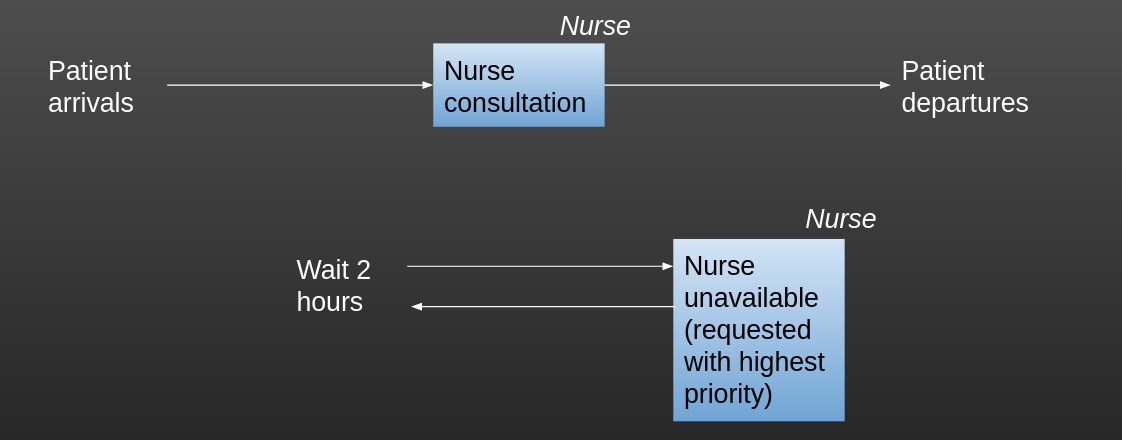
\includegraphics{images/modelling_unavailability.png}

\section{The approach}\label{the-approach}

Basically, we will : - Set up the frequency and duration of
unavailability as parameter values in g class - Make sure that the nurse
is set up as a PriorityResource - Create a new entity generator whose
sole purpose is to demand the nurse resource with a higher priority than
any patient every 2 hours, and will freeze the nurse with them for 15
minutes (this means the nurse will complete the current patient, they
won't walk out midway through!) - Start this new generator running in
our run method of the Model class.

\section{Coding the approach}\label{coding-the-approach}

\subsection{The g class}\label{the-g-class-3}

In the g class, we have added values to specify how long nurse is
unavailable and at what frequency. Un this example, every 2 hours, the
nurse will be unavailable for 15 minutes.

\begin{Shaded}
\begin{Highlighting}[]
\KeywordTok{class}\NormalTok{ g:}
    \CommentTok{\# Inter{-}arrival times}
\NormalTok{    patient\_inter }\OperatorTok{=} \DecValTok{5}

    \CommentTok{\# Activity times}
\NormalTok{    mean\_n\_consult\_time }\OperatorTok{=} \DecValTok{6}

    \CommentTok{\# Resource numbers}
\NormalTok{    number\_of\_nurses }\OperatorTok{=} \DecValTok{1}

\NormalTok{    unav\_time\_nurse }\OperatorTok{=} \DecValTok{15} \CommentTok{\#\#NEW}
\NormalTok{    unav\_freq\_nurse }\OperatorTok{=} \DecValTok{120} \CommentTok{\#\#NEW}

    \CommentTok{\# Simulation meta parameters}
\NormalTok{    sim\_duration }\OperatorTok{=} \DecValTok{2880}
\NormalTok{    number\_of\_runs }\OperatorTok{=} \DecValTok{1}
\NormalTok{    warm\_up\_period }\OperatorTok{=} \DecValTok{1440}
\end{Highlighting}
\end{Shaded}

\subsection{The Patient class}\label{the-patient-class-3}

The patient class is unchanged.

\subsection{The Model class}\label{the-model-class-3}

\subsubsection{The obstruct\_nurse
method}\label{the-obstruct_nurse-method}

We create a new method within the model class called
\texttt{obstruct\_nurse}.

\begin{tcolorbox}[enhanced jigsaw, colframe=quarto-callout-tip-color-frame, bottomtitle=1mm, breakable, rightrule=.15mm, coltitle=black, colbacktitle=quarto-callout-tip-color!10!white, opacityback=0, leftrule=.75mm, arc=.35mm, toptitle=1mm, title=\textcolor{quarto-callout-tip-color}{\faLightbulb}\hspace{0.5em}{Tip}, titlerule=0mm, colback=white, toprule=.15mm, bottomrule=.15mm, left=2mm, opacitybacktitle=0.6]

Note that here we are using a priority value of -1.

Negative priorities are higher (i.e.~are seen first) compared to higher
priorities; a priority value of -1 will be seen before a priority value
of 1, but a priority value of 1 will be seen before a priority value of
2.

This is a very helpful feature to use to keep your breaktime functions
from clashing with high-priority patients.

\end{tcolorbox}

\begin{Shaded}
\begin{Highlighting}[]
\CommentTok{\#\#NEW}
\CommentTok{\# Generator function to obstruct a nurse resource at specified intervals}
\CommentTok{\# for specified amounts of time}
\KeywordTok{def}\NormalTok{ obstruct\_nurse(}\VariableTok{self}\NormalTok{):}
    \ControlFlowTok{while} \VariableTok{True}\NormalTok{:}
        \BuiltInTok{print}\NormalTok{ (}\SpecialStringTok{f"}\SpecialCharTok{\{}\VariableTok{self}\SpecialCharTok{.}\NormalTok{env}\SpecialCharTok{.}\NormalTok{now}\SpecialCharTok{:.2f\}}\SpecialStringTok{: The nurse will go on a break at around time"}\NormalTok{,}
                \SpecialStringTok{f"}\SpecialCharTok{\{}\NormalTok{(}\VariableTok{self}\NormalTok{.env.now }\OperatorTok{+}\NormalTok{ g.unav\_freq\_nurse)}\SpecialCharTok{:.2f\}}\SpecialStringTok{"}\NormalTok{)}

        \CommentTok{\# The generator first pauses for the frequency period}
        \ControlFlowTok{yield} \VariableTok{self}\NormalTok{.env.timeout(g.unav\_freq\_nurse)}

        \CommentTok{\# Once elapsed, the generator requests (demands?) a nurse with}
        \CommentTok{\# a priority of {-}1.  This ensure it takes priority over any patients}
        \CommentTok{\# (whose priority values start at 1).  But it also means that the}
        \CommentTok{\# nurse won\textquotesingle{}t go on a break until they\textquotesingle{}ve finished with the current}
        \CommentTok{\# patient}
        \ControlFlowTok{with} \VariableTok{self}\NormalTok{.nurse.request(priority}\OperatorTok{={-}}\DecValTok{1}\NormalTok{) }\ImportTok{as}\NormalTok{ req:}
            \ControlFlowTok{yield}\NormalTok{ req}

            \BuiltInTok{print}\NormalTok{ (}\SpecialStringTok{f"}\SpecialCharTok{\{}\VariableTok{self}\SpecialCharTok{.}\NormalTok{env}\SpecialCharTok{.}\NormalTok{now}\SpecialCharTok{:.2f\}}\SpecialStringTok{: The nurse is now on a break and will be back at"}\NormalTok{,}
                    \SpecialStringTok{f"}\SpecialCharTok{\{}\NormalTok{(}\VariableTok{self}\NormalTok{.env.now }\OperatorTok{+}\NormalTok{ g.unav\_time\_nurse)}\SpecialCharTok{:.2f\}}\SpecialStringTok{"}\NormalTok{)}

            \CommentTok{\# Freeze with the nurse held in place for the unavailability}
            \CommentTok{\# time (ie duration of the nurse\textquotesingle{}s break).  Here, both the}
            \CommentTok{\# duration and frequency are fixed, but you could randomly}
            \CommentTok{\# sample them from a distribution too if preferred.}
            \ControlFlowTok{yield} \VariableTok{self}\NormalTok{.env.timeout(g.unav\_time\_nurse)}
\end{Highlighting}
\end{Shaded}

\subsubsection{The run method}\label{the-run-method-2}

In our run method, we now start up the \texttt{obstruct\_nurse} process
in addition to the \texttt{generator\_patient\_arrivals} process.

\begin{Shaded}
\begin{Highlighting}[]
\KeywordTok{def}\NormalTok{ run(}\VariableTok{self}\NormalTok{):}
    \CommentTok{\# Start up DES generators}
    \VariableTok{self}\NormalTok{.env.process(}\VariableTok{self}\NormalTok{.generator\_patient\_arrivals())}
    \CommentTok{\#\#NEW {-} we also need to start up the obstructor generator now too}
    \VariableTok{self}\NormalTok{.env.process(}\VariableTok{self}\NormalTok{.obstruct\_nurse())}

    \CommentTok{\# Run for the duration specified in g class}
    \VariableTok{self}\NormalTok{.env.run(until}\OperatorTok{=}\NormalTok{(g.sim\_duration }\OperatorTok{+}\NormalTok{ g.warm\_up\_period))}

    \CommentTok{\# Calculate results over the run}
    \VariableTok{self}\NormalTok{.calculate\_run\_results()}

    \ControlFlowTok{return} \VariableTok{self}\NormalTok{.results\_df}
\end{Highlighting}
\end{Shaded}

\subsection{The Trial class}\label{the-trial-class-3}

The trial class is unchanged.

\section{The full code}\label{the-full-code-1}

The full code is given below.

\begin{tcolorbox}[enhanced jigsaw, colframe=quarto-callout-note-color-frame, bottomtitle=1mm, breakable, rightrule=.15mm, coltitle=black, colbacktitle=quarto-callout-note-color!10!white, opacityback=0, leftrule=.75mm, arc=.35mm, toptitle=1mm, title=\textcolor{quarto-callout-note-color}{\faInfo}\hspace{0.5em}{Click here to view the full code}, titlerule=0mm, colback=white, toprule=.15mm, bottomrule=.15mm, left=2mm, opacitybacktitle=0.6]

\begin{Shaded}
\begin{Highlighting}[]
\ImportTok{import}\NormalTok{ simpy}
\ImportTok{import}\NormalTok{ random}
\ImportTok{import}\NormalTok{ pandas }\ImportTok{as}\NormalTok{ pd}

\CommentTok{\# Class to store global parameter values.}
\KeywordTok{class}\NormalTok{ g:}
    \CommentTok{\# Inter{-}arrival times}
\NormalTok{    patient\_inter }\OperatorTok{=} \DecValTok{5}

    \CommentTok{\# Activity times}
\NormalTok{    mean\_n\_consult\_time }\OperatorTok{=} \DecValTok{6}

    \CommentTok{\# Resource numbers}
\NormalTok{    number\_of\_nurses }\OperatorTok{=} \DecValTok{1}

    \CommentTok{\#\#NEW {-} added values to specify how long nurse is unavailable and at what}
    \CommentTok{\# frequency (in this example, every 2 hours, the nurse will be unavailable}
    \CommentTok{\# for 15 minutes)}
\NormalTok{    unav\_time\_nurse }\OperatorTok{=} \DecValTok{15}
\NormalTok{    unav\_freq\_nurse }\OperatorTok{=} \DecValTok{120}

    \CommentTok{\# Simulation meta parameters}
\NormalTok{    sim\_duration }\OperatorTok{=} \DecValTok{2880}
\NormalTok{    number\_of\_runs }\OperatorTok{=} \DecValTok{1}
\NormalTok{    warm\_up\_period }\OperatorTok{=} \DecValTok{1440}

\CommentTok{\# Class representing patients coming in to the clinic.}
\KeywordTok{class}\NormalTok{ Patient:}
    \KeywordTok{def} \FunctionTok{\_\_init\_\_}\NormalTok{(}\VariableTok{self}\NormalTok{, p\_id):}
        \VariableTok{self}\NormalTok{.}\BuiltInTok{id} \OperatorTok{=}\NormalTok{ p\_id}
        \VariableTok{self}\NormalTok{.q\_time\_nurse }\OperatorTok{=} \DecValTok{0}
        \VariableTok{self}\NormalTok{.priority }\OperatorTok{=}\NormalTok{ random.randint(}\DecValTok{1}\NormalTok{,}\DecValTok{5}\NormalTok{)}

\CommentTok{\# Class representing our model of the clinic.}
\KeywordTok{class}\NormalTok{ Model:}
    \CommentTok{\# Constructor}
    \KeywordTok{def} \FunctionTok{\_\_init\_\_}\NormalTok{(}\VariableTok{self}\NormalTok{, run\_number):}
        \CommentTok{\# Set up SimPy environment}
        \VariableTok{self}\NormalTok{.env }\OperatorTok{=}\NormalTok{ simpy.Environment()}

        \CommentTok{\# Set up counters to use as entity IDs}
        \VariableTok{self}\NormalTok{.patient\_counter }\OperatorTok{=} \DecValTok{0}

        \CommentTok{\# Set up resources}
        \VariableTok{self}\NormalTok{.nurse }\OperatorTok{=}\NormalTok{ simpy.PriorityResource(}\VariableTok{self}\NormalTok{.env,}
\NormalTok{                                            capacity}\OperatorTok{=}\NormalTok{g.number\_of\_nurses)}

        \CommentTok{\# Set run number from value passed in}
        \VariableTok{self}\NormalTok{.run\_number }\OperatorTok{=}\NormalTok{ run\_number}

        \CommentTok{\# Set up DataFrame to store patient{-}level results}
        \VariableTok{self}\NormalTok{.results\_df }\OperatorTok{=}\NormalTok{ pd.DataFrame()}
        \VariableTok{self}\NormalTok{.results\_df[}\StringTok{"Patient ID"}\NormalTok{] }\OperatorTok{=}\NormalTok{ [}\DecValTok{1}\NormalTok{]}
        \VariableTok{self}\NormalTok{.results\_df[}\StringTok{"Q Time Nurse"}\NormalTok{] }\OperatorTok{=}\NormalTok{ [}\FloatTok{0.0}\NormalTok{]}
        \VariableTok{self}\NormalTok{.results\_df.set\_index(}\StringTok{"Patient ID"}\NormalTok{, inplace}\OperatorTok{=}\VariableTok{True}\NormalTok{)}

        \CommentTok{\# Set up attributes that will store mean queuing times across the run}
        \VariableTok{self}\NormalTok{.mean\_q\_time\_nurse }\OperatorTok{=} \DecValTok{0}

\NormalTok{        random.seed(}\DecValTok{42}\NormalTok{)}

    \CommentTok{\# Generator function that represents the DES generator for patient arrivals}
    \KeywordTok{def}\NormalTok{ generator\_patient\_arrivals(}\VariableTok{self}\NormalTok{):}
        \ControlFlowTok{while} \VariableTok{True}\NormalTok{:}
            \VariableTok{self}\NormalTok{.patient\_counter }\OperatorTok{+=} \DecValTok{1}

\NormalTok{            p }\OperatorTok{=}\NormalTok{ Patient(}\VariableTok{self}\NormalTok{.patient\_counter)}

            \VariableTok{self}\NormalTok{.env.process(}\VariableTok{self}\NormalTok{.attend\_clinic(p))}

\NormalTok{            sampled\_inter }\OperatorTok{=}\NormalTok{ random.expovariate(}\FloatTok{1.0} \OperatorTok{/}\NormalTok{ g.patient\_inter)}

            \ControlFlowTok{yield} \VariableTok{self}\NormalTok{.env.timeout(sampled\_inter)}

    \CommentTok{\#\#NEW}
    \CommentTok{\# Generator function to obstruct a nurse resource at specified intervals}
    \CommentTok{\# for specified amounts of time}
    \KeywordTok{def}\NormalTok{ obstruct\_nurse(}\VariableTok{self}\NormalTok{):}
        \ControlFlowTok{while} \VariableTok{True}\NormalTok{:}
            \BuiltInTok{print}\NormalTok{ (}\SpecialStringTok{f"}\SpecialCharTok{\{}\VariableTok{self}\SpecialCharTok{.}\NormalTok{env}\SpecialCharTok{.}\NormalTok{now}\SpecialCharTok{:.2f\}}\SpecialStringTok{: The nurse will go on a break at around time"}\NormalTok{,}
                   \SpecialStringTok{f"}\SpecialCharTok{\{}\NormalTok{(}\VariableTok{self}\NormalTok{.env.now }\OperatorTok{+}\NormalTok{ g.unav\_freq\_nurse)}\SpecialCharTok{:.2f\}}\SpecialStringTok{"}\NormalTok{)}

            \CommentTok{\# The generator first pauses for the frequency period}
            \ControlFlowTok{yield} \VariableTok{self}\NormalTok{.env.timeout(g.unav\_freq\_nurse)}

            \CommentTok{\# Once elapsed, the generator requests (demands?) a nurse with}
            \CommentTok{\# a priority of {-}1.  This ensure it takes priority over any patients}
            \CommentTok{\# (whose priority values start at 1).  But it also means that the}
            \CommentTok{\# nurse won\textquotesingle{}t go on a break until they\textquotesingle{}ve finished with the current}
            \CommentTok{\# patient}
            \ControlFlowTok{with} \VariableTok{self}\NormalTok{.nurse.request(priority}\OperatorTok{={-}}\DecValTok{1}\NormalTok{) }\ImportTok{as}\NormalTok{ req:}
                \ControlFlowTok{yield}\NormalTok{ req}

                \BuiltInTok{print}\NormalTok{ (}\SpecialStringTok{f"}\SpecialCharTok{\{}\VariableTok{self}\SpecialCharTok{.}\NormalTok{env}\SpecialCharTok{.}\NormalTok{now}\SpecialCharTok{:.2f\}}\SpecialStringTok{: The nurse is now on a break and will be back at"}\NormalTok{,}
                       \SpecialStringTok{f"}\SpecialCharTok{\{}\NormalTok{(}\VariableTok{self}\NormalTok{.env.now }\OperatorTok{+}\NormalTok{ g.unav\_time\_nurse)}\SpecialCharTok{:.2f\}}\SpecialStringTok{"}\NormalTok{)}

                \CommentTok{\# Freeze with the nurse held in place for the unavailability}
                \CommentTok{\# time (ie duration of the nurse\textquotesingle{}s break).  Here, both the}
                \CommentTok{\# duration and frequency are fixed, but you could randomly}
                \CommentTok{\# sample them from a distribution too if preferred.}
                \ControlFlowTok{yield} \VariableTok{self}\NormalTok{.env.timeout(g.unav\_time\_nurse)}

    \CommentTok{\# Generator function representing pathway for patients attending the}
    \CommentTok{\# clinic.}
    \KeywordTok{def}\NormalTok{ attend\_clinic(}\VariableTok{self}\NormalTok{, patient):}
        \CommentTok{\# Nurse consultation activity}
\NormalTok{        start\_q\_nurse }\OperatorTok{=} \VariableTok{self}\NormalTok{.env.now}

        \ControlFlowTok{with} \VariableTok{self}\NormalTok{.nurse.request(priority}\OperatorTok{=}\NormalTok{patient.priority) }\ImportTok{as}\NormalTok{ req:}
            \ControlFlowTok{yield}\NormalTok{ req}

\NormalTok{            end\_q\_nurse }\OperatorTok{=} \VariableTok{self}\NormalTok{.env.now}

\NormalTok{            patient.q\_time\_nurse }\OperatorTok{=}\NormalTok{ end\_q\_nurse }\OperatorTok{{-}}\NormalTok{ start\_q\_nurse}

            \ControlFlowTok{if} \VariableTok{self}\NormalTok{.env.now }\OperatorTok{\textgreater{}}\NormalTok{ g.warm\_up\_period:}
                \VariableTok{self}\NormalTok{.results\_df.at[patient.}\BuiltInTok{id}\NormalTok{, }\StringTok{"Q Time Nurse"}\NormalTok{] }\OperatorTok{=}\NormalTok{ (}
\NormalTok{                    patient.q\_time\_nurse}
\NormalTok{                )}

\NormalTok{            sampled\_nurse\_act\_time }\OperatorTok{=}\NormalTok{ random.expovariate(}\FloatTok{1.0} \OperatorTok{/}
\NormalTok{                                                        g.mean\_n\_consult\_time)}

            \ControlFlowTok{yield} \VariableTok{self}\NormalTok{.env.timeout(sampled\_nurse\_act\_time)}

    \CommentTok{\# Method to calculate and store results over the run}
    \KeywordTok{def}\NormalTok{ calculate\_run\_results(}\VariableTok{self}\NormalTok{):}
        \VariableTok{self}\NormalTok{.results\_df.drop([}\DecValTok{1}\NormalTok{], inplace}\OperatorTok{=}\VariableTok{True}\NormalTok{)}

        \VariableTok{self}\NormalTok{.mean\_q\_time\_nurse }\OperatorTok{=} \VariableTok{self}\NormalTok{.results\_df[}\StringTok{"Q Time Nurse"}\NormalTok{].mean()}

    \CommentTok{\# Method to run a single run of the simulation}
    \KeywordTok{def}\NormalTok{ run(}\VariableTok{self}\NormalTok{):}
        \CommentTok{\# Start up DES generators}
        \VariableTok{self}\NormalTok{.env.process(}\VariableTok{self}\NormalTok{.generator\_patient\_arrivals())}
        \CommentTok{\#\#NEW {-} we also need to start up the obstructor generator now too}
        \VariableTok{self}\NormalTok{.env.process(}\VariableTok{self}\NormalTok{.obstruct\_nurse())}

        \CommentTok{\# Run for the duration specified in g class}
        \VariableTok{self}\NormalTok{.env.run(until}\OperatorTok{=}\NormalTok{(g.sim\_duration }\OperatorTok{+}\NormalTok{ g.warm\_up\_period))}

        \CommentTok{\# Calculate results over the run}
        \VariableTok{self}\NormalTok{.calculate\_run\_results()}

        \ControlFlowTok{return} \VariableTok{self}\NormalTok{.results\_df}

\CommentTok{\# Class representing a Trial for our simulation}
\KeywordTok{class}\NormalTok{ Trial:}
    \CommentTok{\# Constructor}
    \KeywordTok{def}  \FunctionTok{\_\_init\_\_}\NormalTok{(}\VariableTok{self}\NormalTok{):}
        \VariableTok{self}\NormalTok{.df\_trial\_results }\OperatorTok{=}\NormalTok{ pd.DataFrame()}
        \VariableTok{self}\NormalTok{.df\_trial\_results[}\StringTok{"Run Number"}\NormalTok{] }\OperatorTok{=}\NormalTok{ [}\DecValTok{0}\NormalTok{]}
        \VariableTok{self}\NormalTok{.df\_trial\_results[}\StringTok{"Mean Q Time Nurse"}\NormalTok{] }\OperatorTok{=}\NormalTok{ [}\FloatTok{0.0}\NormalTok{]}
        \VariableTok{self}\NormalTok{.df\_trial\_results.set\_index(}\StringTok{"Run Number"}\NormalTok{, inplace}\OperatorTok{=}\VariableTok{True}\NormalTok{)}

    \CommentTok{\# Method to calculate and store means across runs in the trial}
    \KeywordTok{def}\NormalTok{ calculate\_means\_over\_trial(}\VariableTok{self}\NormalTok{):}
        \VariableTok{self}\NormalTok{.mean\_q\_time\_nurse\_trial }\OperatorTok{=}\NormalTok{ (}
            \VariableTok{self}\NormalTok{.df\_trial\_results[}\StringTok{"Mean Q Time Nurse"}\NormalTok{].mean()}
\NormalTok{        )}

    \KeywordTok{def}\NormalTok{ run\_trial(}\VariableTok{self}\NormalTok{):}
        \CommentTok{\# Run the simulation for the number of runs specified in g class.}
        \CommentTok{\# For each run, we create a new instance of the Model class and call its}
        \CommentTok{\# run method, which sets everything else in motion.  Once the run has}
        \CommentTok{\# completed, we grab out the stored run results and store it against}
        \CommentTok{\# the run number in the trial results dataframe. We also return the}
        \CommentTok{\# full patient{-}level dataframes.}

        \CommentTok{\# First, create an empty list for storing our patient{-}level dataframes.}
\NormalTok{        results\_dfs }\OperatorTok{=}\NormalTok{ []}

        \ControlFlowTok{for}\NormalTok{ run }\KeywordTok{in} \BuiltInTok{range}\NormalTok{(g.number\_of\_runs):}
\NormalTok{            my\_model }\OperatorTok{=}\NormalTok{ Model(run)}
\NormalTok{            patient\_level\_results }\OperatorTok{=}\NormalTok{ my\_model.run()}

            \CommentTok{\# First let\textquotesingle{}s record our mean wait time for this run}
            \VariableTok{self}\NormalTok{.df\_trial\_results.loc[run] }\OperatorTok{=}\NormalTok{ [my\_model.mean\_q\_time\_nurse]}

            \CommentTok{\# Next let\textquotesingle{}s work on our patient{-}level results dataframes}
            \CommentTok{\# We start by rounding everything to 2 decimal places}
\NormalTok{            patient\_level\_results }\OperatorTok{=}\NormalTok{ patient\_level\_results.}\BuiltInTok{round}\NormalTok{(}\DecValTok{2}\NormalTok{)}
            \CommentTok{\# Add a new column recording the run}
\NormalTok{            patient\_level\_results[}\StringTok{\textquotesingle{}run\textquotesingle{}}\NormalTok{] }\OperatorTok{=}\NormalTok{ run}
            \CommentTok{\# Now we\textquotesingle{}re just going to add this to our empty list (or, after the first}
            \CommentTok{\# time we loop through, as an extra dataframe in our list)}
\NormalTok{            results\_dfs.append(patient\_level\_results)}

\NormalTok{        all\_results\_patient\_level }\OperatorTok{=}\NormalTok{ pd.concat(results\_dfs)}

        \CommentTok{\# This calculates the attribute self.mean\_q\_time\_nurse\_trial}
        \VariableTok{self}\NormalTok{.calculate\_means\_over\_trial()}

        \CommentTok{\# Once the trial (ie all runs) has completed, return the results}
        \ControlFlowTok{return} \VariableTok{self}\NormalTok{.df\_trial\_results, all\_results\_patient\_level, }\VariableTok{self}\NormalTok{.mean\_q\_time\_nurse\_trial}

    \CommentTok{\# Method to print trial results, including averages across runs}
    \KeywordTok{def}\NormalTok{ print\_trial\_results(}\VariableTok{self}\NormalTok{):}
        \BuiltInTok{print}\NormalTok{ (}\StringTok{"Trial Results"}\NormalTok{)}
        \BuiltInTok{print}\NormalTok{ (}\VariableTok{self}\NormalTok{.df\_trial\_results)}

        \BuiltInTok{print}\NormalTok{ (}\SpecialStringTok{f"Mean Q Nurse : }\SpecialCharTok{\{}\VariableTok{self}\SpecialCharTok{.}\NormalTok{mean\_q\_time\_nurse\_trial}\SpecialCharTok{:.1f\}}\SpecialStringTok{ minutes"}\NormalTok{)}
\end{Highlighting}
\end{Shaded}

\end{tcolorbox}

\section{Evaluating the outputs}\label{evaluating-the-outputs-3}

Let's look at the printed output showing when our nurses were
obstructed.

The first number in each line of output shows the simulation time when
the message was generated.

\begin{verbatim}
0.00: The nurse will go on a break at around time 120.00
120.15: The nurse is now on a break and will be back at 135.15
135.15: The nurse will go on a break at around time 255.15
258.44: The nurse is now on a break and will be back at 273.44
273.44: The nurse will go on a break at around time 393.44
404.26: The nurse is now on a break and will be back at 419.26
419.26: The nurse will go on a break at around time 539.26
540.82: The nurse is now on a break and will be back at 555.82
555.82: The nurse will go on a break at around time 675.82
680.63: The nurse is now on a break and will be back at 695.63
695.63: The nurse will go on a break at around time 815.63
827.06: The nurse is now on a break and will be back at 842.06
842.06: The nurse will go on a break at around time 962.06
968.91: The nurse is now on a break and will be back at 983.91
983.91: The nurse will go on a break at around time 1103.91
1106.20: The nurse is now on a break and will be back at 1121.20
1121.20: The nurse will go on a break at around time 1241.20
1242.30: The nurse is now on a break and will be back at 1257.30
1257.30: The nurse will go on a break at around time 1377.30
1389.51: The nurse is now on a break and will be back at 1404.51
1404.51: The nurse will go on a break at around time 1524.51
1532.18: The nurse is now on a break and will be back at 1547.18
1547.18: The nurse will go on a break at around time 1667.18
1672.09: The nurse is now on a break and will be back at 1687.09
1687.09: The nurse will go on a break at around time 1807.09
1807.86: The nurse is now on a break and will be back at 1822.86
1822.86: The nurse will go on a break at around time 1942.86
1947.64: The nurse is now on a break and will be back at 1962.64
1962.64: The nurse will go on a break at around time 2082.64
2084.27: The nurse is now on a break and will be back at 2099.27
2099.27: The nurse will go on a break at around time 2219.27
2221.93: The nurse is now on a break and will be back at 2236.93
2236.93: The nurse will go on a break at around time 2356.93
2359.05: The nurse is now on a break and will be back at 2374.05
2374.05: The nurse will go on a break at around time 2494.05
2494.42: The nurse is now on a break and will be back at 2509.42
2509.42: The nurse will go on a break at around time 2629.42
2635.29: The nurse is now on a break and will be back at 2650.29
2650.29: The nurse will go on a break at around time 2770.29
2776.28: The nurse is now on a break and will be back at 2791.28
2791.28: The nurse will go on a break at around time 2911.28
2911.72: The nurse is now on a break and will be back at 2926.72
2926.72: The nurse will go on a break at around time 3046.72
3050.18: The nurse is now on a break and will be back at 3065.18
3065.18: The nurse will go on a break at around time 3185.18
3203.13: The nurse is now on a break and will be back at 3218.13
3218.13: The nurse will go on a break at around time 3338.13
3350.63: The nurse is now on a break and will be back at 3365.63
3365.63: The nurse will go on a break at around time 3485.63
3486.03: The nurse is now on a break and will be back at 3501.03
3501.03: The nurse will go on a break at around time 3621.03
3623.49: The nurse is now on a break and will be back at 3638.49
3638.49: The nurse will go on a break at around time 3758.49
3768.95: The nurse is now on a break and will be back at 3783.95
3783.95: The nurse will go on a break at around time 3903.95
3908.67: The nurse is now on a break and will be back at 3923.67
3923.67: The nurse will go on a break at around time 4043.67
4045.96: The nurse is now on a break and will be back at 4060.96
4060.96: The nurse will go on a break at around time 4180.96
4184.07: The nurse is now on a break and will be back at 4199.07
4199.07: The nurse will go on a break at around time 4319.07
\end{verbatim}

Now let's look at some of the other outputs and compare them with a
version without the nurse obstruction.

Now let's look at some of the other outputs and compare them with a
version without the nurse obstruction.

\begin{verbatim}
The average wait when there are no nurse breaks is 143.18 minutes
\end{verbatim}

\begin{verbatim}
The average wait when there are nurse breaks is 299.7 minutes
\end{verbatim}

\chapter{Choosing Distributions}\label{sec-distributions}

In the previous session, we mentioned that whilst it's a useful tip to
start by having all of the distributions in our model be Exponential
(because it's easy to tweak an Exponential Distribution), for real world
models we probably want to then adapt them to use a Lognormal
Distribution for activity times.

A Lognormal Distribution is commonly used in Discrete Event simulation
to model the time to perform a task. It is \textbf{right-skewed}, which
basically means it has a long tail. To put it in more understandable
terms, it suggests that most activity times will be similar, but some
will be longer, and some will be MUCH longer. This tends to capture
activity times in patient pathways well.

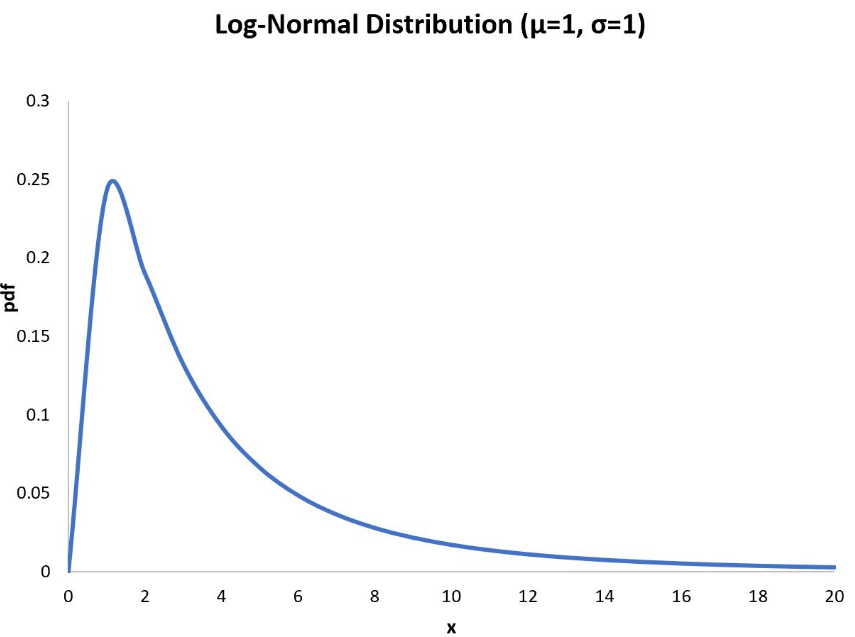
\includegraphics{images/lognormal.png}

\section{A bit of background}\label{a-bit-of-background}

\begin{tcolorbox}[enhanced jigsaw, colframe=quarto-callout-tip-color-frame, bottomtitle=1mm, breakable, rightrule=.15mm, coltitle=black, colbacktitle=quarto-callout-tip-color!10!white, opacityback=0, leftrule=.75mm, arc=.35mm, toptitle=1mm, title=\textcolor{quarto-callout-tip-color}{\faLightbulb}\hspace{0.5em}{Tip}, titlerule=0mm, colback=white, toprule=.15mm, bottomrule=.15mm, left=2mm, opacitybacktitle=0.6]

The good news is that we will be using some prewritten code to specify
our lognormal, and all we will need to know to do this is the mean
(average) time for our activity, and the standard deviation (a measure
of how much the times vary across the dataset that python can calculate
for us if given a list of activity times).

However - it's useful to have a bit more of an idea about what a
lognormal is - so do have a read of the section below, but if you don't
quite get it just yet, don't fret - just remember that lognormal is good
for activity times in general, and the exponential distribution is good
for inter-arrival times (the time between patients arriving).

\end{tcolorbox}

\subsection{The normal distribution}\label{the-normal-distribution}

A normal distribution is a bell shaped curve that is symmetrical. It is
defined by two parameters : μ (Mu) and σ (Sigma), which represent the
mean and standard deviation of the distribution. So it's easy to plug in
such values from our own data.

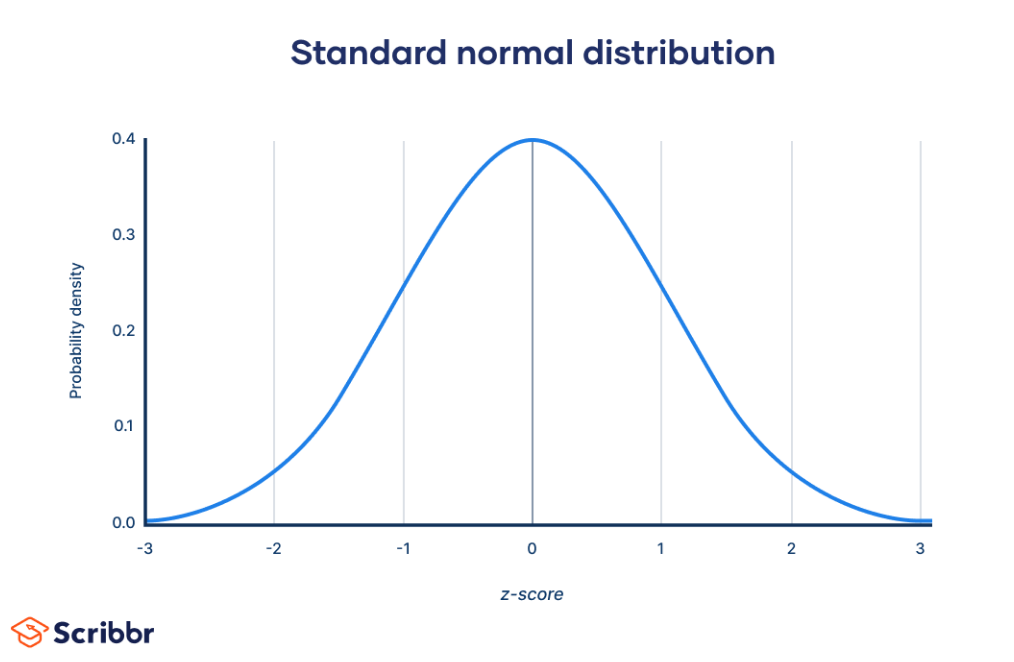
\includegraphics{images/normal_dist.png}

\subsection{Logarithms}\label{logarithms}

Before we proceed, let's remind ourselves about something many of us
learned at school (and then promptly forgot) : Logarithms.

Logarithms are basically the opposite of exponentials.

Effectively, lognormals relate to how many copies of one number multiply
together to make another number.

How many 4s multiply together to make 64?

4 x 4 x 4 = 64 We had to multiply 3 copies of the number 4 to get 64.

This means that the logarithm is 3.

We'd write this as \[
Y = log_4(64) = 3
\]

\subsection{Bringing it all together - lognormal
distributions}\label{bringing-it-all-together---lognormal-distributions}

How does this relate to the distribution?

Well, a Lognormal distribution is one in which the \textbf{logarithm} of
the random variable we're modelling is normally distributed.

This means that the the two parameters μ (Mu) and σ (Sigma) used to
specify a Lognormal distribution do not represent the mean and standard
deviation, unlike the normal distribution; rather, they represent what
are known as the location and scale of the distribution respectively.

μ (Mu) and σ (Sigma) represent the mean and standard deviation once the
data in the log normal distribution has been transformed using
logarithms.

It's easy to get the mean and standard deviation of our data.

If we used the Normal distribution, we could do that.

\begin{tcolorbox}[enhanced jigsaw, colframe=quarto-callout-warning-color-frame, bottomtitle=1mm, breakable, rightrule=.15mm, coltitle=black, colbacktitle=quarto-callout-warning-color!10!white, opacityback=0, leftrule=.75mm, arc=.35mm, toptitle=1mm, title=\textcolor{quarto-callout-warning-color}{\faExclamationTriangle}\hspace{0.5em}{Warning}, titlerule=0mm, colback=white, toprule=.15mm, bottomrule=.15mm, left=2mm, opacitybacktitle=0.6]

The Normal distribution often isn't good for activity times - it allows
negative values - activity distributions are rarely symmetrical -
they're more likely to be a bit `wonky' (skewed), with just a few
activities being much longer

\end{tcolorbox}

The probalm is we can't just give a Lognormal distribution the mean and
standard deviation, because in a Lognormal distribution, the mean and
standard deviation of our data is represented in the underlying normal
distribution not the Lognormal distribution (remember, it's the
logarithms of the values that are normally distributed).

\begin{tcolorbox}[enhanced jigsaw, colframe=quarto-callout-tip-color-frame, bottomtitle=1mm, breakable, rightrule=.15mm, coltitle=black, colbacktitle=quarto-callout-tip-color!10!white, opacityback=0, leftrule=.75mm, arc=.35mm, toptitle=1mm, title=\textcolor{quarto-callout-tip-color}{\faLightbulb}\hspace{0.5em}{Tip}, titlerule=0mm, colback=white, toprule=.15mm, bottomrule=.15mm, left=2mm, opacitybacktitle=0.6]

\textbf{So what do we do?}

We need to convert our mean and standard deviation values (that we get
from our real world data) into Mu and Sigma for a Lognormal
distribution.

\textbf{This is the key bit you need to understand!}

\end{tcolorbox}

\section{Code for the lognormal
distribution}\label{code-for-the-lognormal-distribution}

This code was written by
\href{https://orcid.org/0000-0003-2631-4481}{Tom Monks}.

\begin{Shaded}
\begin{Highlighting}[]
\ImportTok{import}\NormalTok{ numpy }\ImportTok{as}\NormalTok{ np}
\ImportTok{import}\NormalTok{ math}

\KeywordTok{class}\NormalTok{ Lognormal:}
    \CommentTok{"""}
\CommentTok{    Encapsulates a lognormal distirbution}
\CommentTok{    """}
    \KeywordTok{def} \FunctionTok{\_\_init\_\_}\NormalTok{(}\VariableTok{self}\NormalTok{, mean, stdev, random\_seed}\OperatorTok{=}\VariableTok{None}\NormalTok{):}
        \CommentTok{"""}
\CommentTok{        Params:}
\CommentTok{        {-}{-}{-}{-}{-}{-}{-}}
\CommentTok{        mean = mean of the lognormal distribution}
\CommentTok{        stdev = standard dev of the lognormal distribution}
\CommentTok{        """}
        \VariableTok{self}\NormalTok{.rand }\OperatorTok{=}\NormalTok{ np.random.default\_rng(seed}\OperatorTok{=}\NormalTok{random\_seed)}
\NormalTok{        mu, sigma }\OperatorTok{=} \VariableTok{self}\NormalTok{.normal\_moments\_from\_lognormal(mean, stdev}\OperatorTok{**}\DecValTok{2}\NormalTok{)}
        \VariableTok{self}\NormalTok{.mu }\OperatorTok{=}\NormalTok{ mu}
        \VariableTok{self}\NormalTok{.sigma }\OperatorTok{=}\NormalTok{ sigma}

    \KeywordTok{def}\NormalTok{ normal\_moments\_from\_lognormal(}\VariableTok{self}\NormalTok{, m, v):}
        \CommentTok{\textquotesingle{}\textquotesingle{}\textquotesingle{}}
\CommentTok{        Returns mu and sigma of normal distribution}
\CommentTok{        underlying a lognormal with mean m and variance v}
\CommentTok{        source: https://blogs.sas.com/content/iml/2014/06/04/simulate{-}lognormal}
\CommentTok{        {-}data{-}with{-}specified{-}mean{-}and{-}variance.html}

\CommentTok{        Params:}
\CommentTok{        {-}{-}{-}{-}{-}{-}{-}}
\CommentTok{        m = mean of lognormal distribution}
\CommentTok{        v = variance of lognormal distribution}

\CommentTok{        Returns:}
\CommentTok{        {-}{-}{-}{-}{-}{-}{-}}
\CommentTok{        (float, float)}
\CommentTok{        \textquotesingle{}\textquotesingle{}\textquotesingle{}}
\NormalTok{        phi }\OperatorTok{=}\NormalTok{ math.sqrt(v }\OperatorTok{+}\NormalTok{ m}\OperatorTok{**}\DecValTok{2}\NormalTok{)}
\NormalTok{        mu }\OperatorTok{=}\NormalTok{ math.log(m}\OperatorTok{**}\DecValTok{2}\OperatorTok{/}\NormalTok{phi)}
\NormalTok{        sigma }\OperatorTok{=}\NormalTok{ math.sqrt(math.log(phi}\OperatorTok{**}\DecValTok{2}\OperatorTok{/}\NormalTok{m}\OperatorTok{**}\DecValTok{2}\NormalTok{))}
        \ControlFlowTok{return}\NormalTok{ mu, sigma}

    \KeywordTok{def}\NormalTok{ sample(}\VariableTok{self}\NormalTok{):}
        \CommentTok{"""}
\CommentTok{        Sample from the normal distribution}
\CommentTok{        """}
        \ControlFlowTok{return} \VariableTok{self}\NormalTok{.rand.lognormal(}\VariableTok{self}\NormalTok{.mu, }\VariableTok{self}\NormalTok{.sigma)}
\end{Highlighting}
\end{Shaded}

We will add this into our model code.

Then we just need to make sure we have both a mean and standard
deviation (SD) for activity times that we want to represent on Lognormal
distributions

When we need to sample an activity time, we create an instance of the
Lognormal class with our mean and SD, and call the sample method.

We are going to do this in the attend\_clinic method of the Model class.

\begin{Shaded}
\begin{Highlighting}[]
\KeywordTok{def}\NormalTok{ attend\_clinic(}\VariableTok{self}\NormalTok{, patient):}
        \CommentTok{\# Nurse consultation activity}
\NormalTok{        start\_q\_nurse }\OperatorTok{=} \VariableTok{self}\NormalTok{.env.now}

        \ControlFlowTok{with} \VariableTok{self}\NormalTok{.nurse.request(priority}\OperatorTok{=}\NormalTok{patient.priority) }\ImportTok{as}\NormalTok{ req:}
            \ControlFlowTok{yield}\NormalTok{ req}

\NormalTok{            end\_q\_nurse }\OperatorTok{=} \VariableTok{self}\NormalTok{.env.now}

\NormalTok{            patient.q\_time\_nurse }\OperatorTok{=}\NormalTok{ end\_q\_nurse }\OperatorTok{{-}}\NormalTok{ start\_q\_nurse}

            \ControlFlowTok{if} \VariableTok{self}\NormalTok{.env.now }\OperatorTok{\textgreater{}}\NormalTok{ g.warm\_up\_period:}
                \VariableTok{self}\NormalTok{.results\_df.at[patient.}\BuiltInTok{id}\NormalTok{, }\StringTok{"Q Time Nurse"}\NormalTok{] }\OperatorTok{=}\NormalTok{ (}
\NormalTok{                    patient.q\_time\_nurse}
\NormalTok{                )}

            \CommentTok{\#\#NEW {-} we now use a lognormal distribution for the activity time,}
            \CommentTok{\# so we create an instance of our Lognormal class with the mean}
            \CommentTok{\# and standard deviations specified in g class, and then sample}
            \CommentTok{\# from it (we do this in a single line of code here, much as we}
            \CommentTok{\# did when sampling from the exponential distribution before).}
\NormalTok{            sampled\_nurse\_act\_time }\OperatorTok{=}\NormalTok{ Lognormal(}
\NormalTok{                g.mean\_n\_consult\_time, g.sd\_n\_consult\_time).sample()}

            \ControlFlowTok{yield} \VariableTok{self}\NormalTok{.env.timeout(sampled\_nurse\_act\_time)}
\end{Highlighting}
\end{Shaded}

\section{Additional distributions}\label{additional-distributions}

In fact, there are many different distributions available.

The sim-tools package makes it easy to make use of them without having
to write lots of classes yourself.

The source code for the package can be investigated in its
\href{https://github.com/TomMonks/sim-tools}{Github Repository}.

To install the package, run

\begin{Shaded}
\begin{Highlighting}[]
\NormalTok{pip install sim}\OperatorTok{{-}}\NormalTok{tools}
\end{Highlighting}
\end{Shaded}

You can then import a class with

\begin{Shaded}
\begin{Highlighting}[]
\ImportTok{from}\NormalTok{ sim\_tools.distributions }\ImportTok{import}\NormalTok{ Exponential}
\end{Highlighting}
\end{Shaded}

replacing Exponential with any of the supported distribution classes.

An overview of how to use the classes, and of the different
distributions included, is embedded below:

\chapter{Reproducibility}\label{sec-reproducibility}

One great thing about DES is controlled randomness.

Now, computers aren't very good at being completely random!

What we do is give it a `seed' to start from when we are sampling from a
distribution..

If our seed is 1, maybe the arrival times sampled from the distribution
will be

5 minutes, 2 minutes, 3 minutes, 6 minutes, 5 minutes

If our seed is 101, maybe the arrival times will be

10 minutes, 2 minutes, 5 minutes, 5 minutes, 3 minutes

Why is this good?

We can either - Change the random number and see how the same system can
cope with different patterns of arrivals - Keep the random number the
same and see how changing the system affects performance

Let's go back to our branching model.

At the moment, we have not set a \textbf{seed} anywhere explicitly.

What the \textbf{random} package will do is default the seed to being
the date and time that the code is run at - this helps to ensure the
results are random, but this can then cause us some problems.

When we do 100 runs, change the parameters (say add an extra nurse) and
then do another 100 runs, we don't currently know how much of the
difference in results is due to the change in system (the extra nurse),
and how much is due to random variation in the number and timing of
arrivals, how long their consultations take, and the chance of them
going on to the second consultation.

So let's set a \textbf{random seed} so that we \emph{fix} the patterns
and arrivals.

\section{Exploring ways of coding in
reproducibility}\label{exploring-ways-of-coding-in-reproducibility}

\begin{tcolorbox}[enhanced jigsaw, colframe=quarto-callout-warning-color-frame, bottomtitle=1mm, breakable, rightrule=.15mm, coltitle=black, colbacktitle=quarto-callout-warning-color!10!white, opacityback=0, leftrule=.75mm, arc=.35mm, toptitle=1mm, title=\textcolor{quarto-callout-warning-color}{\faExclamationTriangle}\hspace{0.5em}{Warning}, titlerule=0mm, colback=white, toprule=.15mm, bottomrule=.15mm, left=2mm, opacitybacktitle=0.6]

The method shown in this section has limitations - but reading through
this section will help you understand more about seeds and why the
method in Section~\ref{sec-robust} (``A robust way to ensure controlled
randomness'') is better.

\end{tcolorbox}

The best place to do this is in our trial class.

In our run\_trial method within that class, we can set the seed so that
it matches the run number.

This will ensure each run has a different seed, but that the seed is the
same across different runs.

\begin{Shaded}
\begin{Highlighting}[]
\KeywordTok{def}\NormalTok{ run\_trial(}\VariableTok{self}\NormalTok{):}
    \CommentTok{\# Run the simulation for the number of runs specified in g class.}
    \CommentTok{\# For each run, we create a new instance of the Model class and call its}
    \CommentTok{\# run method, which sets everything else in motion.  Once the run has}
    \CommentTok{\# completed, we grab out the stored run results (just mean queuing time}
    \CommentTok{\# here) and store it against the run number in the trial results}
    \CommentTok{\# dataframe.}
    \ControlFlowTok{for}\NormalTok{ run }\KeywordTok{in} \BuiltInTok{range}\NormalTok{(g.number\_of\_runs):}
\NormalTok{        random.seed(run)}

\NormalTok{        my\_model }\OperatorTok{=}\NormalTok{ Model(run)}
\NormalTok{        my\_model.run()}

        \VariableTok{self}\NormalTok{.df\_trial\_results.loc[run] }\OperatorTok{=}\NormalTok{ [my\_model.mean\_q\_time\_recep,}
\NormalTok{                                          my\_model.mean\_q\_time\_nurse,}
\NormalTok{                                          my\_model.mean\_q\_time\_doctor]}

    \CommentTok{\# Once the trial (ie all runs) has completed, print the final results}
    \VariableTok{self}\NormalTok{.print\_trial\_results()}
\end{Highlighting}
\end{Shaded}

Let's look at the output now.

Let's run 100 trials and look at the outputs.

\begin{Shaded}
\begin{Highlighting}[]
\CommentTok{\# Create an instance of the Trial class}
\NormalTok{my\_trial }\OperatorTok{=}\NormalTok{ Trial()}

\CommentTok{\# Call the run\_trial method of our Trial object}
\NormalTok{my\_trial.run\_trial()}
\end{Highlighting}
\end{Shaded}

\begin{verbatim}
Trial Results
            Arrivals  Mean Q Time Recep  Mean Q Time Nurse  Mean Q Time Doctor
Run Number                                                                    
0              105.0               0.48               6.77               51.94
1              117.0               0.90              89.23               10.82
2              110.0               1.86              27.21               33.57
3              115.0               0.92              78.11               55.77
4              104.0               1.52              46.56               94.60
...              ...                ...                ...                 ...
95             127.0               0.62              96.29               69.36
96             132.0               1.01              54.03               34.93
97             126.0               2.20              67.00               76.15
98             152.0               1.67              89.61               10.58
99             112.0               0.70              22.13               82.26

[100 rows x 4 columns]
Arrivals              120.44
Mean Q Time Recep       1.31
Mean Q Time Nurse      64.46
Mean Q Time Doctor     35.10
dtype: float64
\end{verbatim}

Now let's run 100 trials again. Are the results the same?

Let's run 100 trials and look at the outputs.

\begin{Shaded}
\begin{Highlighting}[]
\CommentTok{\# Create an instance of the Trial class}
\NormalTok{my\_trial }\OperatorTok{=}\NormalTok{ Trial()}

\CommentTok{\# Call the run\_trial method of our Trial object}
\NormalTok{my\_trial.run\_trial()}
\end{Highlighting}
\end{Shaded}

\begin{verbatim}
Trial Results
            Arrivals  Mean Q Time Recep  Mean Q Time Nurse  Mean Q Time Doctor
Run Number                                                                    
0              105.0               0.48               6.77               51.94
1              117.0               0.90              89.23               10.82
2              110.0               1.86              27.21               33.57
3              115.0               0.92              78.11               55.77
4              104.0               1.52              46.56               94.60
...              ...                ...                ...                 ...
95             127.0               0.62              96.29               69.36
96             132.0               1.01              54.03               34.93
97             126.0               2.20              67.00               76.15
98             152.0               1.67              89.61               10.58
99             112.0               0.70              22.13               82.26

[100 rows x 4 columns]
Arrivals              120.44
Mean Q Time Recep       1.31
Mean Q Time Nurse      64.46
Mean Q Time Doctor     35.10
dtype: float64
\end{verbatim}

Yes!

Now let's compare this when we start changing the number of nurses.

This is going to change the queue times for nurses and, by extension,
for doctors (as people will be turning up to the doctors at different
times).

However, the number of arrivals should remain unchanged.

\begin{verbatim}
Trial Results
            Arrivals  Mean Q Time Recep  Mean Q Time Nurse  Mean Q Time Doctor
Run Number                                                                    
0              105.0               0.48               6.77               51.94
1              117.0               0.90              89.23               10.82
2              110.0               1.86              27.21               33.57
3              115.0               0.92              78.11               55.77
4              104.0               1.52              46.56               94.60
...              ...                ...                ...                 ...
95             127.0               0.62              96.29               69.36
96             132.0               1.01              54.03               34.93
97             126.0               2.20              67.00               76.15
98             152.0               1.67              89.61               10.58
99             112.0               0.70              22.13               82.26

[100 rows x 4 columns]
Arrivals              120.44
Mean Q Time Recep       1.31
Mean Q Time Nurse      64.46
Mean Q Time Doctor     35.10
dtype: float64
\end{verbatim}

\begin{verbatim}
Trial Results
            Arrivals  Mean Q Time Recep  Mean Q Time Nurse  Mean Q Time Doctor
Run Number                                                                    
0              106.0               0.96               0.78               52.59
1               99.0               0.43               2.29               22.72
2              116.0               2.96               2.84               93.46
3              123.0               0.86               1.27               57.58
4              114.0               2.40               3.53               68.42
...              ...                ...                ...                 ...
95             123.0               1.39               3.73               45.02
96             138.0               0.97               1.95              102.04
97             116.0               1.33               2.34               24.49
98             125.0               1.07               1.59               40.84
99             129.0               1.47               5.90               17.22

[100 rows x 4 columns]
Arrivals              118.39
Mean Q Time Recep       1.23
Mean Q Time Nurse       2.98
Mean Q Time Doctor     53.23
dtype: float64
\end{verbatim}

Unfortunately, what we wanted (and needed) to happen, hasn't.

Instead, we are seeing that the number of arrivals are changing too.

\begin{tcolorbox}[enhanced jigsaw, colframe=quarto-callout-note-color-frame, bottomtitle=1mm, breakable, rightrule=.15mm, coltitle=black, colbacktitle=quarto-callout-note-color!10!white, opacityback=0, leftrule=.75mm, arc=.35mm, toptitle=1mm, title=\textcolor{quarto-callout-note-color}{\faInfo}\hspace{0.5em}{Note}, titlerule=0mm, colback=white, toprule=.15mm, bottomrule=.15mm, left=2mm, opacitybacktitle=0.6]

This is because of the way random number generation occurs.

The order the random numbers are generated in matters - and as the order
of events changes (in this case, as we have more nurses, they can see
more patients quicker, changing the order that subsequent events happen
in).

Let's investigate this with two examples.

\begin{Shaded}
\begin{Highlighting}[]
\NormalTok{random.seed(}\DecValTok{42}\NormalTok{)}

\BuiltInTok{print}\NormalTok{(}\SpecialStringTok{f"1: inter{-}arrival time 1 }\SpecialCharTok{\{}\NormalTok{random}\SpecialCharTok{.}\NormalTok{expovariate(}\FloatTok{1.0} \OperatorTok{/}\NormalTok{ g.patient\_inter)}\SpecialCharTok{:.2f\}}\SpecialStringTok{"}\NormalTok{)}
\BuiltInTok{print}\NormalTok{(}\SpecialStringTok{f"3: inter{-}arrival time 2 }\SpecialCharTok{\{}\NormalTok{random}\SpecialCharTok{.}\NormalTok{expovariate(}\FloatTok{1.0} \OperatorTok{/}\NormalTok{ g.patient\_inter)}\SpecialCharTok{:.2f\}}\SpecialStringTok{"}\NormalTok{)}
\BuiltInTok{print}\NormalTok{(}\SpecialStringTok{f"2: reception consult time 1 }\SpecialCharTok{\{}\NormalTok{random}\SpecialCharTok{.}\NormalTok{expovariate(}\FloatTok{1.0} \OperatorTok{/}\NormalTok{ g.mean\_reception\_time)}\SpecialCharTok{:.2f\}}\SpecialStringTok{"}\NormalTok{)}
\BuiltInTok{print}\NormalTok{(}\SpecialStringTok{f"4: inter{-}arrival time 3 }\SpecialCharTok{\{}\NormalTok{random}\SpecialCharTok{.}\NormalTok{expovariate(}\FloatTok{1.0} \OperatorTok{/}\NormalTok{ g.patient\_inter)}\SpecialCharTok{:.2f\}}\SpecialStringTok{"}\NormalTok{)}
\end{Highlighting}
\end{Shaded}

\begin{verbatim}
1: inter-arrival time 1 5.10
3: inter-arrival time 2 0.13
2: reception consult time 1 0.64
4: inter-arrival time 3 1.26
\end{verbatim}

\begin{Shaded}
\begin{Highlighting}[]
\NormalTok{random.seed(}\DecValTok{42}\NormalTok{)}

\BuiltInTok{print}\NormalTok{(}\SpecialStringTok{f"1: inter{-}arrival time 1 }\SpecialCharTok{\{}\NormalTok{random}\SpecialCharTok{.}\NormalTok{expovariate(}\FloatTok{1.0} \OperatorTok{/}\NormalTok{ g.patient\_inter)}\SpecialCharTok{:.2f\}}\SpecialStringTok{"}\NormalTok{)}
\BuiltInTok{print}\NormalTok{(}\SpecialStringTok{f"2: inter{-}arrival time 2 }\SpecialCharTok{\{}\NormalTok{random}\SpecialCharTok{.}\NormalTok{expovariate(}\FloatTok{1.0} \OperatorTok{/}\NormalTok{ g.patient\_inter)}\SpecialCharTok{:.2f\}}\SpecialStringTok{"}\NormalTok{)}
\BuiltInTok{print}\NormalTok{(}\SpecialStringTok{f"4: inter{-}arrival time 3 }\SpecialCharTok{\{}\NormalTok{random}\SpecialCharTok{.}\NormalTok{expovariate(}\FloatTok{1.0} \OperatorTok{/}\NormalTok{ g.patient\_inter)}\SpecialCharTok{:.2f\}}\SpecialStringTok{"}\NormalTok{)}
\BuiltInTok{print}\NormalTok{(}\SpecialStringTok{f"3: reception consult time  1 }\SpecialCharTok{\{}\NormalTok{random}\SpecialCharTok{.}\NormalTok{expovariate(}\FloatTok{1.0} \OperatorTok{/}\NormalTok{ g.mean\_reception\_time)}\SpecialCharTok{:.2f\}}\SpecialStringTok{"}\NormalTok{)}
\end{Highlighting}
\end{Shaded}

\begin{verbatim}
1: inter-arrival time 1 5.10
2: inter-arrival time 2 0.13
4: inter-arrival time 3 1.61
3: reception consult time  1 0.51
\end{verbatim}

We can see that the first two inter-arrival times are consistent.
However, when we swap the order of generating the next inter-arrival
time and generating a length of time for someone to spend with a
receptionist, we see that the times are different.

\end{tcolorbox}

\begin{tcolorbox}[enhanced jigsaw, colframe=quarto-callout-warning-color-frame, bottomtitle=1mm, breakable, rightrule=.15mm, coltitle=black, colbacktitle=quarto-callout-warning-color!10!white, opacityback=0, leftrule=.75mm, arc=.35mm, toptitle=1mm, title=\textcolor{quarto-callout-warning-color}{\faExclamationTriangle}\hspace{0.5em}{Warning}, titlerule=0mm, colback=white, toprule=.15mm, bottomrule=.15mm, left=2mm, opacitybacktitle=0.6]

So while this method is ok just to ensure that a single output remains
consistent when you rerun your analysis, it's no good for ensuring
you're making good comparisons across different simulation scenarios.

So how can we do this?

\end{tcolorbox}

\section{A robust way to ensure controlled randomness}\label{sec-robust}

Effectively, we want separate seeds for the random number generator for
\textbf{each separate type of event we are generating random numbers
for}.

This means that we have separate random number streams for the different
parts of our process - our inter-arrival times - our consult times - our
probabilities

The easiest way to implement this is to switch from using the
\texttt{random} library to using the distributions provided in simtools.

We will replace \texttt{random.expovariate} with the
\texttt{Exponential} class.

First, we need to import this class.

\begin{Shaded}
\begin{Highlighting}[]
\ImportTok{from}\NormalTok{ sim\_tools.distributions }\ImportTok{import}\NormalTok{ Exponential}
\end{Highlighting}
\end{Shaded}

We now set up the distributions when initialising the model.

\begin{Shaded}
\begin{Highlighting}[]
\KeywordTok{class}\NormalTok{ Model:}
    \CommentTok{\# Constructor to set up the model for a run.  We pass in a run number when}
    \CommentTok{\# we create a new model.}
    \KeywordTok{def} \FunctionTok{\_\_init\_\_}\NormalTok{(}\VariableTok{self}\NormalTok{, run\_number):}
        \CommentTok{\# Create a SimPy environment in which everything will live}
        \VariableTok{self}\NormalTok{.env }\OperatorTok{=}\NormalTok{ simpy.Environment()}

        \CommentTok{\# Create a patient counter (which we\textquotesingle{}ll use as a patient ID)}
        \VariableTok{self}\NormalTok{.patient\_counter }\OperatorTok{=} \DecValTok{0}

        \CommentTok{\# Create our resources}
        \VariableTok{self}\NormalTok{.receptionist }\OperatorTok{=}\NormalTok{ simpy.Resource(}
            \VariableTok{self}\NormalTok{.env, capacity}\OperatorTok{=}\NormalTok{g.number\_of\_receptionists}
\NormalTok{        )}
        \VariableTok{self}\NormalTok{.nurse }\OperatorTok{=}\NormalTok{ simpy.Resource(}\VariableTok{self}\NormalTok{.env, capacity}\OperatorTok{=}\NormalTok{g.number\_of\_nurses)}
        \VariableTok{self}\NormalTok{.doctor }\OperatorTok{=}\NormalTok{ simpy.Resource(}
            \VariableTok{self}\NormalTok{.env, capacity}\OperatorTok{=}\NormalTok{g.number\_of\_doctors)}

        \CommentTok{\# Store the passed in run number}
        \VariableTok{self}\NormalTok{.run\_number }\OperatorTok{=}\NormalTok{ run\_number}

        \CommentTok{\# Create a new Pandas DataFrame that will store some results against}
        \CommentTok{\# the patient ID (which we\textquotesingle{}ll use as the index).}
        \VariableTok{self}\NormalTok{.results\_df }\OperatorTok{=}\NormalTok{ pd.DataFrame()}
        \VariableTok{self}\NormalTok{.results\_df[}\StringTok{"Patient ID"}\NormalTok{] }\OperatorTok{=}\NormalTok{ [}\DecValTok{1}\NormalTok{]}
        \VariableTok{self}\NormalTok{.results\_df[}\StringTok{"Q Time Recep"}\NormalTok{] }\OperatorTok{=}\NormalTok{ [}\FloatTok{0.0}\NormalTok{]}
        \VariableTok{self}\NormalTok{.results\_df[}\StringTok{"Time with Recep"}\NormalTok{] }\OperatorTok{=}\NormalTok{ [}\FloatTok{0.0}\NormalTok{]}
        \VariableTok{self}\NormalTok{.results\_df[}\StringTok{"Q Time Nurse"}\NormalTok{] }\OperatorTok{=}\NormalTok{ [}\FloatTok{0.0}\NormalTok{]}
        \VariableTok{self}\NormalTok{.results\_df[}\StringTok{"Time with Nurse"}\NormalTok{] }\OperatorTok{=}\NormalTok{ [}\FloatTok{0.0}\NormalTok{]}
        \VariableTok{self}\NormalTok{.results\_df[}\StringTok{"Q Time Doctor"}\NormalTok{] }\OperatorTok{=}\NormalTok{ [}\FloatTok{0.0}\NormalTok{]}
        \VariableTok{self}\NormalTok{.results\_df[}\StringTok{"Time with Doctor"}\NormalTok{] }\OperatorTok{=}\NormalTok{ [}\FloatTok{0.0}\NormalTok{]}
        \VariableTok{self}\NormalTok{.results\_df.set\_index(}\StringTok{"Patient ID"}\NormalTok{, inplace}\OperatorTok{=}\VariableTok{True}\NormalTok{)}

        \CommentTok{\# Create an attribute to store the mean queuing times across this run of}
        \CommentTok{\# the model}
        \VariableTok{self}\NormalTok{.mean\_q\_time\_recep }\OperatorTok{=} \DecValTok{0}
        \VariableTok{self}\NormalTok{.mean\_q\_time\_nurse }\OperatorTok{=} \DecValTok{0}
        \VariableTok{self}\NormalTok{.mean\_q\_time\_doctor }\OperatorTok{=} \DecValTok{0}

        \CommentTok{\#\#NEW {-} initialise distributions}
        \VariableTok{self}\NormalTok{.patient\_inter\_arrival\_dist }\OperatorTok{=}\NormalTok{ Exponential(mean }\OperatorTok{=}\NormalTok{ g.patient\_inter, random\_seed }\OperatorTok{=} \VariableTok{self}\NormalTok{.run\_number}\OperatorTok{*}\DecValTok{2}\NormalTok{)}
        \VariableTok{self}\NormalTok{.patient\_reception\_time\_dist }\OperatorTok{=}\NormalTok{ Exponential(mean }\OperatorTok{=}\NormalTok{ g.mean\_reception\_time, random\_seed }\OperatorTok{=} \VariableTok{self}\NormalTok{.run\_number}\OperatorTok{*}\DecValTok{3}\NormalTok{)}
        \VariableTok{self}\NormalTok{.nurse\_consult\_time\_dist }\OperatorTok{=}\NormalTok{ Exponential(mean }\OperatorTok{=}\NormalTok{ g.mean\_n\_consult\_time, random\_seed }\OperatorTok{=} \VariableTok{self}\NormalTok{.run\_number}\OperatorTok{*}\DecValTok{4}\NormalTok{)}
        \VariableTok{self}\NormalTok{.doctor\_consult\_time\_dist }\OperatorTok{=}\NormalTok{ Exponential(mean }\OperatorTok{=}\NormalTok{ g.mean\_d\_consult\_time, random\_seed }\OperatorTok{=} \VariableTok{self}\NormalTok{.run\_number}\OperatorTok{*}\DecValTok{5}\NormalTok{)}
\end{Highlighting}
\end{Shaded}

\begin{tcolorbox}[enhanced jigsaw, colframe=quarto-callout-warning-color-frame, bottomtitle=1mm, breakable, rightrule=.15mm, coltitle=black, colbacktitle=quarto-callout-warning-color!10!white, opacityback=0, leftrule=.75mm, arc=.35mm, toptitle=1mm, title=\textcolor{quarto-callout-warning-color}{\faExclamationTriangle}\hspace{0.5em}{Warning}, titlerule=0mm, colback=white, toprule=.15mm, bottomrule=.15mm, left=2mm, opacitybacktitle=0.6]

Note that the value we pass to initialise the Exponential variable here
is \textbf{just the mean time}.

When we were using random.expovariate, we passed 1 dividided by the mean
time.

\end{tcolorbox}

Next, everywhere we have previously used \texttt{random.expovariate}, we
replace this with the .sample() method of our newly initialised
distributions.

For example

\begin{Shaded}
\begin{Highlighting}[]
\NormalTok{sampled\_doctor\_act\_time }\OperatorTok{=}\NormalTok{ random.expovariate(}
    \FloatTok{1.0} \OperatorTok{/}\NormalTok{ g.mean\_d\_consult\_time}
\NormalTok{)}
\end{Highlighting}
\end{Shaded}

becomes

\begin{Shaded}
\begin{Highlighting}[]
\NormalTok{sampled\_doctor\_act\_time }\OperatorTok{=} \VariableTok{self}\NormalTok{.doctor\_consult\_time\_dist.sample()}
\end{Highlighting}
\end{Shaded}

\subsection{The full code}\label{the-full-code-2}

Let's update all the code and run our previous experiment again.

\begin{tcolorbox}[enhanced jigsaw, colframe=quarto-callout-note-color-frame, bottomtitle=1mm, breakable, rightrule=.15mm, coltitle=black, colbacktitle=quarto-callout-note-color!10!white, opacityback=0, leftrule=.75mm, arc=.35mm, toptitle=1mm, title=\textcolor{quarto-callout-note-color}{\faInfo}\hspace{0.5em}{Click here to view the full code}, titlerule=0mm, colback=white, toprule=.15mm, bottomrule=.15mm, left=2mm, opacitybacktitle=0.6]

\begin{Shaded}
\begin{Highlighting}[]
\ImportTok{import}\NormalTok{ simpy}
\ImportTok{import}\NormalTok{ random}
\ImportTok{import}\NormalTok{ pandas }\ImportTok{as}\NormalTok{ pd}
\ImportTok{from}\NormalTok{ sim\_tools.distributions }\ImportTok{import}\NormalTok{ Exponential }\CommentTok{\#\#NEW}

\CommentTok{\# Class to store global parameter values.  We don\textquotesingle{}t create an instance of this}
\CommentTok{\# class {-} we just refer to the class blueprint itself to access the numbers}
\CommentTok{\# inside.}
\KeywordTok{class}\NormalTok{ g:}
\NormalTok{    patient\_inter }\OperatorTok{=} \DecValTok{5}
\NormalTok{    mean\_reception\_time }\OperatorTok{=} \DecValTok{2}
\NormalTok{    mean\_n\_consult\_time }\OperatorTok{=} \DecValTok{6}
\NormalTok{    mean\_d\_consult\_time }\OperatorTok{=} \DecValTok{20}
\NormalTok{    number\_of\_receptionists }\OperatorTok{=} \DecValTok{1}
\NormalTok{    number\_of\_nurses }\OperatorTok{=} \DecValTok{1}
\NormalTok{    number\_of\_doctors }\OperatorTok{=} \DecValTok{2}
\NormalTok{    prob\_seeing\_doctor }\OperatorTok{=} \FloatTok{0.6}
\NormalTok{    sim\_duration }\OperatorTok{=} \DecValTok{600}
\NormalTok{    number\_of\_runs }\OperatorTok{=} \DecValTok{100}

\CommentTok{\# Class representing patients coming in to the clinic.}
\KeywordTok{class}\NormalTok{ Patient:}
    \KeywordTok{def} \FunctionTok{\_\_init\_\_}\NormalTok{(}\VariableTok{self}\NormalTok{, p\_id):}
        \VariableTok{self}\NormalTok{.}\BuiltInTok{id} \OperatorTok{=}\NormalTok{ p\_id}
        \VariableTok{self}\NormalTok{.q\_time\_recep }\OperatorTok{=} \DecValTok{0}
        \VariableTok{self}\NormalTok{.q\_time\_nurse }\OperatorTok{=} \DecValTok{0}
        \VariableTok{self}\NormalTok{.q\_time\_doctor }\OperatorTok{=} \DecValTok{0}

\CommentTok{\# Class representing our model of the clinic.}
\KeywordTok{class}\NormalTok{ Model:}
    \CommentTok{\# Constructor to set up the model for a run.  We pass in a run number when}
    \CommentTok{\# we create a new model.}
    \KeywordTok{def} \FunctionTok{\_\_init\_\_}\NormalTok{(}\VariableTok{self}\NormalTok{, run\_number):}
        \CommentTok{\# Create a SimPy environment in which everything will live}
        \VariableTok{self}\NormalTok{.env }\OperatorTok{=}\NormalTok{ simpy.Environment()}

        \CommentTok{\# Create a patient counter (which we\textquotesingle{}ll use as a patient ID)}
        \VariableTok{self}\NormalTok{.patient\_counter }\OperatorTok{=} \DecValTok{0}

        \CommentTok{\# Create our resources}
        \VariableTok{self}\NormalTok{.receptionist }\OperatorTok{=}\NormalTok{ simpy.Resource(}
            \VariableTok{self}\NormalTok{.env, capacity}\OperatorTok{=}\NormalTok{g.number\_of\_receptionists}
\NormalTok{        )}
        \VariableTok{self}\NormalTok{.nurse }\OperatorTok{=}\NormalTok{ simpy.Resource(}\VariableTok{self}\NormalTok{.env, capacity}\OperatorTok{=}\NormalTok{g.number\_of\_nurses)}
        \VariableTok{self}\NormalTok{.doctor }\OperatorTok{=}\NormalTok{ simpy.Resource(}
            \VariableTok{self}\NormalTok{.env, capacity}\OperatorTok{=}\NormalTok{g.number\_of\_doctors)}

        \CommentTok{\# Store the passed in run number}
        \VariableTok{self}\NormalTok{.run\_number }\OperatorTok{=}\NormalTok{ run\_number}

        \CommentTok{\# Create a new Pandas DataFrame that will store some results against}
        \CommentTok{\# the patient ID (which we\textquotesingle{}ll use as the index).}
        \VariableTok{self}\NormalTok{.results\_df }\OperatorTok{=}\NormalTok{ pd.DataFrame()}
        \VariableTok{self}\NormalTok{.results\_df[}\StringTok{"Patient ID"}\NormalTok{] }\OperatorTok{=}\NormalTok{ [}\DecValTok{1}\NormalTok{]}
        \VariableTok{self}\NormalTok{.results\_df[}\StringTok{"Q Time Recep"}\NormalTok{] }\OperatorTok{=}\NormalTok{ [}\FloatTok{0.0}\NormalTok{]}
        \VariableTok{self}\NormalTok{.results\_df[}\StringTok{"Time with Recep"}\NormalTok{] }\OperatorTok{=}\NormalTok{ [}\FloatTok{0.0}\NormalTok{]}
        \VariableTok{self}\NormalTok{.results\_df[}\StringTok{"Q Time Nurse"}\NormalTok{] }\OperatorTok{=}\NormalTok{ [}\FloatTok{0.0}\NormalTok{]}
        \VariableTok{self}\NormalTok{.results\_df[}\StringTok{"Time with Nurse"}\NormalTok{] }\OperatorTok{=}\NormalTok{ [}\FloatTok{0.0}\NormalTok{]}
        \VariableTok{self}\NormalTok{.results\_df[}\StringTok{"Q Time Doctor"}\NormalTok{] }\OperatorTok{=}\NormalTok{ [}\FloatTok{0.0}\NormalTok{]}
        \VariableTok{self}\NormalTok{.results\_df[}\StringTok{"Time with Doctor"}\NormalTok{] }\OperatorTok{=}\NormalTok{ [}\FloatTok{0.0}\NormalTok{]}
        \VariableTok{self}\NormalTok{.results\_df.set\_index(}\StringTok{"Patient ID"}\NormalTok{, inplace}\OperatorTok{=}\VariableTok{True}\NormalTok{)}

        \CommentTok{\# Create an attribute to store the mean queuing times across this run of}
        \CommentTok{\# the model}
        \VariableTok{self}\NormalTok{.mean\_q\_time\_recep }\OperatorTok{=} \DecValTok{0}
        \VariableTok{self}\NormalTok{.mean\_q\_time\_nurse }\OperatorTok{=} \DecValTok{0}
        \VariableTok{self}\NormalTok{.mean\_q\_time\_doctor }\OperatorTok{=} \DecValTok{0}

        \VariableTok{self}\NormalTok{.patient\_inter\_arrival\_dist }\OperatorTok{=}\NormalTok{ Exponential(mean }\OperatorTok{=}\NormalTok{ g.patient\_inter, random\_seed }\OperatorTok{=} \VariableTok{self}\NormalTok{.run\_number}\OperatorTok{*}\DecValTok{2}\NormalTok{)}
        \VariableTok{self}\NormalTok{.patient\_reception\_time\_dist }\OperatorTok{=}\NormalTok{ Exponential(mean }\OperatorTok{=}\NormalTok{ g.mean\_reception\_time, random\_seed }\OperatorTok{=} \VariableTok{self}\NormalTok{.run\_number}\OperatorTok{*}\DecValTok{3}\NormalTok{)}
        \VariableTok{self}\NormalTok{.nurse\_consult\_time\_dist }\OperatorTok{=}\NormalTok{ Exponential(mean }\OperatorTok{=}\NormalTok{ g.mean\_n\_consult\_time, random\_seed }\OperatorTok{=} \VariableTok{self}\NormalTok{.run\_number}\OperatorTok{*}\DecValTok{4}\NormalTok{)}
        \VariableTok{self}\NormalTok{.doctor\_consult\_time\_dist }\OperatorTok{=}\NormalTok{ Exponential(mean }\OperatorTok{=}\NormalTok{ g.mean\_d\_consult\_time, random\_seed }\OperatorTok{=} \VariableTok{self}\NormalTok{.run\_number}\OperatorTok{*}\DecValTok{5}\NormalTok{)}

    \CommentTok{\# A generator function that represents the DES generator for patient}
    \CommentTok{\# arrivals}
    \KeywordTok{def}\NormalTok{ generator\_patient\_arrivals(}\VariableTok{self}\NormalTok{):}
        \CommentTok{\# We use an infinite loop here to keep doing this indefinitely whilst}
        \CommentTok{\# the simulation runs}
        \ControlFlowTok{while} \VariableTok{True}\NormalTok{:}
            \CommentTok{\# Increment the patient counter by 1 (this means our first patient}
            \CommentTok{\# will have an ID of 1)}
            \VariableTok{self}\NormalTok{.patient\_counter }\OperatorTok{+=} \DecValTok{1}

            \CommentTok{\# Create a new patient {-} an instance of the Patient Class we}
            \CommentTok{\# defined above.  Remember, we pass in the ID when creating a}
            \CommentTok{\# patient {-} so here we pass the patient counter to use as the ID.}
\NormalTok{            p }\OperatorTok{=}\NormalTok{ Patient(}\VariableTok{self}\NormalTok{.patient\_counter)}

            \CommentTok{\# Tell SimPy to start up the attend\_clinic generator function with}
            \CommentTok{\# this patient (the generator function that will model the}
            \CommentTok{\# patient\textquotesingle{}s journey through the system)}
            \VariableTok{self}\NormalTok{.env.process(}\VariableTok{self}\NormalTok{.attend\_clinic(p))}

            \CommentTok{\# Randomly sample the time to the next patient arriving.  Here, we}
            \CommentTok{\# sample from an exponential distribution (common for inter{-}arrival}
            \CommentTok{\# times), and pass in a lambda value of 1 / mean.  The mean}
            \CommentTok{\# inter{-}arrival time is stored in the g class.}
\NormalTok{            sampled\_inter }\OperatorTok{=} \VariableTok{self}\NormalTok{.patient\_inter\_arrival\_dist.sample() }\CommentTok{\#\#NEW}

            \CommentTok{\# Freeze this instance of this function in place until the}
            \CommentTok{\# inter{-}arrival time we sampled above has elapsed.  Note {-} time in}
            \CommentTok{\# SimPy progresses in "Time Units", which can represent anything}
            \CommentTok{\# you like (just make sure you\textquotesingle{}re consistent within the model)}
            \ControlFlowTok{yield} \VariableTok{self}\NormalTok{.env.timeout(sampled\_inter)}

    \CommentTok{\# A generator function that represents the pathway for a patient going}
    \CommentTok{\# through the clinic.}
    \CommentTok{\# The patient object is passed in to the generator function so we can}
    \CommentTok{\# extract information from / record information to it}
    \KeywordTok{def}\NormalTok{ attend\_clinic(}\VariableTok{self}\NormalTok{, patient):}
\NormalTok{        start\_q\_recep }\OperatorTok{=} \VariableTok{self}\NormalTok{.env.now}

        \ControlFlowTok{with} \VariableTok{self}\NormalTok{.receptionist.request() }\ImportTok{as}\NormalTok{ req:}
            \ControlFlowTok{yield}\NormalTok{ req}

\NormalTok{            end\_q\_recep }\OperatorTok{=} \VariableTok{self}\NormalTok{.env.now}

\NormalTok{            patient.q\_time\_recep }\OperatorTok{=}\NormalTok{ end\_q\_recep }\OperatorTok{{-}}\NormalTok{ start\_q\_recep}

\NormalTok{            sampled\_recep\_act\_time }\OperatorTok{=} \VariableTok{self}\NormalTok{.patient\_reception\_time\_dist.sample() }\CommentTok{\#\#NEW}

            \VariableTok{self}\NormalTok{.results\_df.at[patient.}\BuiltInTok{id}\NormalTok{, }\StringTok{"Q Time Recep"}\NormalTok{] }\OperatorTok{=}\NormalTok{ (}
\NormalTok{                 patient.q\_time\_recep}
\NormalTok{            )}
            \VariableTok{self}\NormalTok{.results\_df.at[patient.}\BuiltInTok{id}\NormalTok{, }\StringTok{"Time with Recep"}\NormalTok{] }\OperatorTok{=}\NormalTok{ (}
\NormalTok{                 sampled\_recep\_act\_time}
\NormalTok{            )}

            \ControlFlowTok{yield} \VariableTok{self}\NormalTok{.env.timeout(sampled\_recep\_act\_time)}

        \CommentTok{\# Here\textquotesingle{}s where the patient finishes with the receptionist, and starts}
        \CommentTok{\# queuing for the nurse}

        \CommentTok{\# Record the time the patient started queuing for a nurse}
\NormalTok{        start\_q\_nurse }\OperatorTok{=} \VariableTok{self}\NormalTok{.env.now}

        \CommentTok{\# This code says request a nurse resource, and do all of the following}
        \CommentTok{\# block of code with that nurse resource held in place (and therefore}
        \CommentTok{\# not usable by another patient)}
        \ControlFlowTok{with} \VariableTok{self}\NormalTok{.nurse.request() }\ImportTok{as}\NormalTok{ req:}
            \CommentTok{\# Freeze the function until the request for a nurse can be met.}
            \CommentTok{\# The patient is currently queuing.}
            \ControlFlowTok{yield}\NormalTok{ req}

            \CommentTok{\# When we get to this bit of code, control has been passed back to}
            \CommentTok{\# the generator function, and therefore the request for a nurse has}
            \CommentTok{\# been met.  We now have the nurse, and have stopped queuing, so we}
            \CommentTok{\# can record the current time as the time we finished queuing.}
\NormalTok{            end\_q\_nurse }\OperatorTok{=} \VariableTok{self}\NormalTok{.env.now}

            \CommentTok{\# Calculate the time this patient was queuing for the nurse, and}
            \CommentTok{\# record it in the patient\textquotesingle{}s attribute for this.}
\NormalTok{            patient.q\_time\_nurse }\OperatorTok{=}\NormalTok{ end\_q\_nurse }\OperatorTok{{-}}\NormalTok{ start\_q\_nurse}

            \CommentTok{\# Now we\textquotesingle{}ll randomly sample the time this patient with the nurse.}
            \CommentTok{\# Here, we use an Exponential distribution for simplicity, but you}
            \CommentTok{\# would typically use a Log Normal distribution for a real model}
            \CommentTok{\# (we\textquotesingle{}ll come back to that).  As with sampling the inter{-}arrival}
            \CommentTok{\# times, we grab the mean from the g class, and pass in 1 / mean}
            \CommentTok{\# as the lambda value.}
\NormalTok{            sampled\_nurse\_act\_time }\OperatorTok{=} \VariableTok{self}\NormalTok{.nurse\_consult\_time\_dist.sample() }\CommentTok{\#\#NEW}

            \CommentTok{\# Here we\textquotesingle{}ll store the queuing time for the nurse and the sampled}
            \CommentTok{\# time to spend with the nurse in the results DataFrame against the}
            \CommentTok{\# ID for this patient.  In real world models, you may not want to}
            \CommentTok{\# bother storing the sampled activity times {-} but as this is a}
            \CommentTok{\# simple model, we\textquotesingle{}ll do it here.}
            \CommentTok{\# We use a handy property of pandas called .at, which works a bit}
            \CommentTok{\# like .loc.  .at allows us to access (and therefore change) a}
            \CommentTok{\# particular cell in our DataFrame by providing the row and column.}
            \CommentTok{\# Here, we specify the row as the patient ID (the index), and the}
            \CommentTok{\# column for the value we want to update for that patient.}
            \VariableTok{self}\NormalTok{.results\_df.at[patient.}\BuiltInTok{id}\NormalTok{, }\StringTok{"Q Time Nurse"}\NormalTok{] }\OperatorTok{=}\NormalTok{ (}
\NormalTok{                patient.q\_time\_nurse)}
            \VariableTok{self}\NormalTok{.results\_df.at[patient.}\BuiltInTok{id}\NormalTok{, }\StringTok{"Time with Nurse"}\NormalTok{] }\OperatorTok{=}\NormalTok{ (}
\NormalTok{                sampled\_nurse\_act\_time)}

            \CommentTok{\# Freeze this function in place for the activity time we sampled}
            \CommentTok{\# above.  This is the patient spending time with the nurse.}
            \ControlFlowTok{yield} \VariableTok{self}\NormalTok{.env.timeout(sampled\_nurse\_act\_time)}

            \CommentTok{\# When the time above elapses, the generator function will return}
            \CommentTok{\# here.  As there\textquotesingle{}s nothing more that we\textquotesingle{}ve written, the function}
            \CommentTok{\# will simply end.  This is a sink.  We could choose to add}
            \CommentTok{\# something here if we wanted to record something {-} e.g. a counter}
            \CommentTok{\# for number of patients that left, recording something about the}
            \CommentTok{\# patients that left at a particular sink etc.}

        \CommentTok{\# Conditional logic to see if patient goes on to see doctor}
        \CommentTok{\# We sample from the uniform distribution between 0 and 1.  If the value}
        \CommentTok{\# is less than the probability of seeing a doctor (stored in g Class)}
        \CommentTok{\# then we say the patient sees a doctor.}
        \CommentTok{\# If not, this block of code won\textquotesingle{}t be run and the patient will just}
        \CommentTok{\# leave the system (we could add in an else if we wanted a branching}
        \CommentTok{\# path to another activity instead)}
        \ControlFlowTok{if}\NormalTok{ random.uniform(}\DecValTok{0}\NormalTok{,}\DecValTok{1}\NormalTok{) }\OperatorTok{\textless{}}\NormalTok{ g.prob\_seeing\_doctor:}
\NormalTok{            start\_q\_doctor }\OperatorTok{=} \VariableTok{self}\NormalTok{.env.now}

            \ControlFlowTok{with} \VariableTok{self}\NormalTok{.doctor.request() }\ImportTok{as}\NormalTok{ req:}
                \ControlFlowTok{yield}\NormalTok{ req}

\NormalTok{                end\_q\_doctor }\OperatorTok{=} \VariableTok{self}\NormalTok{.env.now}

\NormalTok{                patient.q\_time\_doctor }\OperatorTok{=}\NormalTok{ end\_q\_doctor }\OperatorTok{{-}}\NormalTok{ start\_q\_doctor}

\NormalTok{                sampled\_doctor\_act\_time }\OperatorTok{=} \VariableTok{self}\NormalTok{.nurse\_consult\_time\_dist.sample() }\CommentTok{\#\#NEW}

                \VariableTok{self}\NormalTok{.results\_df.at[patient.}\BuiltInTok{id}\NormalTok{, }\StringTok{"Q Time Doctor"}\NormalTok{] }\OperatorTok{=}\NormalTok{ (}
\NormalTok{                    patient.q\_time\_doctor}
\NormalTok{                )}
                \VariableTok{self}\NormalTok{.results\_df.at[patient.}\BuiltInTok{id}\NormalTok{, }\StringTok{"Time with Doctor"}\NormalTok{] }\OperatorTok{=}\NormalTok{ (}
\NormalTok{                    sampled\_doctor\_act\_time}
\NormalTok{                )}

                \ControlFlowTok{yield} \VariableTok{self}\NormalTok{.env.timeout(sampled\_doctor\_act\_time)}

    \CommentTok{\# This method calculates results over a single run.  Here we just calculate}
    \CommentTok{\# a mean, but in real world models you\textquotesingle{}d probably want to calculate more.}
    \KeywordTok{def}\NormalTok{ calculate\_run\_results(}\VariableTok{self}\NormalTok{):}
        \CommentTok{\# Take the mean of the queuing times across patients in this run of the}
        \CommentTok{\# model.}
        \VariableTok{self}\NormalTok{.mean\_q\_time\_recep }\OperatorTok{=} \VariableTok{self}\NormalTok{.results\_df[}\StringTok{"Q Time Recep"}\NormalTok{].mean()}
        \VariableTok{self}\NormalTok{.mean\_q\_time\_nurse }\OperatorTok{=} \VariableTok{self}\NormalTok{.results\_df[}\StringTok{"Q Time Nurse"}\NormalTok{].mean()}
        \VariableTok{self}\NormalTok{.mean\_q\_time\_doctor }\OperatorTok{=} \VariableTok{self}\NormalTok{.results\_df[}\StringTok{"Q Time Doctor"}\NormalTok{].mean()}

    \CommentTok{\# The run method starts up the DES entity generators, runs the simulation,}
    \CommentTok{\# and in turns calls anything we need to generate results for the run}
    \KeywordTok{def}\NormalTok{ run(}\VariableTok{self}\NormalTok{):}
        \CommentTok{\# Start up our DES entity generators that create new patients.  We\textquotesingle{}ve}
        \CommentTok{\# only got one in this model, but we\textquotesingle{}d need to do this for each one if}
        \CommentTok{\# we had multiple generators.}
        \VariableTok{self}\NormalTok{.env.process(}\VariableTok{self}\NormalTok{.generator\_patient\_arrivals())}

        \CommentTok{\# Run the model for the duration specified in g class}
        \VariableTok{self}\NormalTok{.env.run(until}\OperatorTok{=}\NormalTok{g.sim\_duration)}

        \CommentTok{\# Now the simulation run has finished, call the method that calculates}
        \CommentTok{\# run results}
        \VariableTok{self}\NormalTok{.calculate\_run\_results()}

        \CommentTok{\# Print the run number with the patient{-}level results from this run of}
        \CommentTok{\# the model}
        \ControlFlowTok{return}\NormalTok{ (}\VariableTok{self}\NormalTok{.results\_df)}

\CommentTok{\# Class representing a Trial for our simulation {-} a batch of simulation runs.}
\KeywordTok{class}\NormalTok{ Trial:}
    \CommentTok{\# The constructor sets up a pandas dataframe that will store the key}
    \CommentTok{\# results from each run against run number, with run number as the index.}
    \KeywordTok{def}  \FunctionTok{\_\_init\_\_}\NormalTok{(}\VariableTok{self}\NormalTok{):}
        \VariableTok{self}\NormalTok{.df\_trial\_results }\OperatorTok{=}\NormalTok{ pd.DataFrame()}
        \VariableTok{self}\NormalTok{.df\_trial\_results[}\StringTok{"Run Number"}\NormalTok{] }\OperatorTok{=}\NormalTok{ [}\DecValTok{0}\NormalTok{]}
        \VariableTok{self}\NormalTok{.df\_trial\_results[}\StringTok{"Arrivals"}\NormalTok{] }\OperatorTok{=}\NormalTok{ [}\DecValTok{0}\NormalTok{]}
        \VariableTok{self}\NormalTok{.df\_trial\_results[}\StringTok{"Mean Q Time Recep"}\NormalTok{] }\OperatorTok{=}\NormalTok{ [}\FloatTok{0.0}\NormalTok{]}
        \VariableTok{self}\NormalTok{.df\_trial\_results[}\StringTok{"Mean Q Time Nurse"}\NormalTok{] }\OperatorTok{=}\NormalTok{ [}\FloatTok{0.0}\NormalTok{]}
        \VariableTok{self}\NormalTok{.df\_trial\_results[}\StringTok{"Mean Q Time Doctor"}\NormalTok{] }\OperatorTok{=}\NormalTok{ [}\FloatTok{0.0}\NormalTok{]}
        \VariableTok{self}\NormalTok{.df\_trial\_results.set\_index(}\StringTok{"Run Number"}\NormalTok{, inplace}\OperatorTok{=}\VariableTok{True}\NormalTok{)}

    \CommentTok{\# Method to print out the results from the trial.  In real world models,}
    \CommentTok{\# you\textquotesingle{}d likely save them as well as (or instead of) printing them}
    \KeywordTok{def}\NormalTok{ print\_trial\_results(}\VariableTok{self}\NormalTok{):}
        \BuiltInTok{print}\NormalTok{ (}\StringTok{"Trial Results"}\NormalTok{)}
        \BuiltInTok{print}\NormalTok{ (}\VariableTok{self}\NormalTok{.df\_trial\_results.}\BuiltInTok{round}\NormalTok{(}\DecValTok{2}\NormalTok{))}
        \BuiltInTok{print}\NormalTok{(}\VariableTok{self}\NormalTok{.df\_trial\_results.mean().}\BuiltInTok{round}\NormalTok{(}\DecValTok{2}\NormalTok{))}

    \CommentTok{\# Method to run a trial}
    \KeywordTok{def}\NormalTok{ run\_trial(}\VariableTok{self}\NormalTok{):}
        \BuiltInTok{print}\NormalTok{(}\SpecialStringTok{f"}\SpecialCharTok{\{}\NormalTok{g}\SpecialCharTok{.}\NormalTok{number\_of\_receptionists}\SpecialCharTok{\}}\SpecialStringTok{ receptionists, }\SpecialCharTok{\{}\NormalTok{g}\SpecialCharTok{.}\NormalTok{number\_of\_nurses}\SpecialCharTok{\}}\SpecialStringTok{ nurses, }\SpecialCharTok{\{}\NormalTok{g}\SpecialCharTok{.}\NormalTok{number\_of\_doctors}\SpecialCharTok{\}}\SpecialStringTok{ doctors"}\NormalTok{) }\CommentTok{\#\# NEW}
        \BuiltInTok{print}\NormalTok{(}\StringTok{""}\NormalTok{) }\CommentTok{\#\# NEW: Print a blank line}
        \CommentTok{\# Run the simulation for the number of runs specified in g class.}
        \CommentTok{\# For each run, we create a new instance of the Model class and call its}
        \CommentTok{\# run method, which sets everything else in motion.  Once the run has}
        \CommentTok{\# completed, we grab out the stored run results (just mean queuing time}
        \CommentTok{\# here) and store it against the run number in the trial results}
        \CommentTok{\# dataframe.}
        \ControlFlowTok{for}\NormalTok{ run }\KeywordTok{in} \BuiltInTok{range}\NormalTok{(g.number\_of\_runs):}
\NormalTok{            random.seed(run)}

\NormalTok{            my\_model }\OperatorTok{=}\NormalTok{ Model(run)}
\NormalTok{            patient\_level\_results }\OperatorTok{=}\NormalTok{ my\_model.run()}

            \VariableTok{self}\NormalTok{.df\_trial\_results.loc[run] }\OperatorTok{=}\NormalTok{ [}
                \BuiltInTok{len}\NormalTok{(patient\_level\_results),}
\NormalTok{                my\_model.mean\_q\_time\_recep,}
\NormalTok{                my\_model.mean\_q\_time\_nurse,}
\NormalTok{                my\_model.mean\_q\_time\_doctor}
\NormalTok{                ]}

        \CommentTok{\# Once the trial (ie all runs) has completed, print the final results}
        \VariableTok{self}\NormalTok{.print\_trial\_results()}
\end{Highlighting}
\end{Shaded}

\end{tcolorbox}

\subsection{Evaluating the outputs}\label{evaluating-the-outputs-4}

\begin{verbatim}
1 receptionists, 1 nurses, 2 doctors

Trial Results
            Arrivals  Mean Q Time Recep  Mean Q Time Nurse  Mean Q Time Doctor
Run Number                                                                    
0              102.0               0.00              57.19                1.15
1              125.0               1.84             144.69                0.02
2              112.0               0.85              15.30                1.13
3              120.0               1.08              82.67                0.04
4              132.0               1.94             107.47                0.51
...              ...                ...                ...                 ...
95              91.0               0.35               9.08                0.15
96             122.0               1.09              63.11                0.32
97              97.0               0.58              21.86                0.10
98             133.0               1.86             124.94                0.09
99             122.0               0.57              63.14                0.66

[100 rows x 4 columns]
Arrivals              122.39
Mean Q Time Recep       1.27
Mean Q Time Nurse      61.35
Mean Q Time Doctor      0.48
dtype: float64
\end{verbatim}

\begin{verbatim}
1 receptionists, 2 nurses, 2 doctors

Trial Results
            Arrivals  Mean Q Time Recep  Mean Q Time Nurse  Mean Q Time Doctor
Run Number                                                                    
0              102.0               0.00               2.49                1.01
1              125.0               1.84               3.55                1.56
2              112.0               0.85               3.61                0.59
3              120.0               1.08               3.43                0.19
4              132.0               1.94               4.20                0.91
...              ...                ...                ...                 ...
95              91.0               0.35               1.08                0.07
96             122.0               1.09               2.20                0.73
97              97.0               0.58               1.09                1.04
98             133.0               1.86               4.19                1.41
99             122.0               0.57               1.86                0.85

[100 rows x 4 columns]
Arrivals              122.39
Mean Q Time Recep       1.27
Mean Q Time Nurse       2.97
Mean Q Time Doctor      0.89
dtype: float64
\end{verbatim}

With these changes made, we can see that the number of arrivals and the
queue time for the receptionists across the trials has remained
consistent, while the waits for nurses and doctors have changed, but we
can now be confident that this is because of alterations to the
parameters - not uncontrolled randomness.

\chapter{Multiple Entity Types Following The Same (or Very Similar)
Pathways}\label{multiple-entity-types-following-the-same-or-very-similar-pathways}

Let's now make our model more complex by adding in some additional
patient classes.

What we do here will scale to any number of entity types.

\section{The Approach}\label{the-approach-1}

\begin{tcolorbox}[enhanced jigsaw, colframe=quarto-callout-tip-color-frame, bottomtitle=1mm, breakable, rightrule=.15mm, coltitle=black, colbacktitle=quarto-callout-tip-color!10!white, opacityback=0, leftrule=.75mm, arc=.35mm, toptitle=1mm, title=\textcolor{quarto-callout-tip-color}{\faLightbulb}\hspace{0.5em}{Tip}, titlerule=0mm, colback=white, toprule=.15mm, bottomrule=.15mm, left=2mm, opacitybacktitle=0.6]

The basic rule of thumb is have different generators if the entities
(and / or what happens to them) is different if they come in via a
different route

\end{tcolorbox}

However, before we kick off, it will save us time down the road if we
first improve the way the model handles \textbf{randomness}. Full
details can be found in the \href{./reproducibility.qmd}{reproducibility
chapter}, but we will cover the key changes in this section as well.

In short, what we will do in our model is

\begin{itemize}
\tightlist
\item
  move the setup of our sampling distributions into our model class
\item
  add additional attributes to our g class for our different types of
  patients
\item
  create multiple generators that will cause our different patient types
  to arrive at the appropriate rate
\end{itemize}

\begin{tcolorbox}[enhanced jigsaw, colframe=quarto-callout-note-color-frame, bottomtitle=1mm, breakable, rightrule=.15mm, coltitle=black, colbacktitle=quarto-callout-note-color!10!white, opacityback=0, leftrule=.75mm, arc=.35mm, toptitle=1mm, title=\textcolor{quarto-callout-note-color}{\faInfo}\hspace{0.5em}{Note}, titlerule=0mm, colback=white, toprule=.15mm, bottomrule=.15mm, left=2mm, opacitybacktitle=0.6]

There are different approaches you can take to having multiple types of
entities - this is one of the situations in which the flexiblity of
Python and SimPy start to become apparent, and there isn't necessarily
one `right' way.

For example, let's imagine a scenario where we have two types of patient
arriving at different rates - let's split them into `seriously injured'
and `mildly injured'.

\subsection{Approaches to Managing
Arrivals}\label{approaches-to-managing-arrivals}

We could filter our historical data by patient type, work out the
inter-arrival time between the `seriously injured' patients and set up a
generator for these patients, and then repeat this for the `mildly
injured' patients.

However - you could instead have stuck with a single generator, like in
our previous approach, but instead sampled whether the incoming patient
is a

\subsection{Approaches to Patient
Classes}\label{approaches-to-patient-classes}

Similarly, when it comes to our patient classes, there are multiple ways
we could handle it.

We could use the concept of inheritance to have a main patient class,
then have multiple `child' classes who inherit the properties of the
parent class while also recording their own special , with the different
processes generating the relevant patient type.

However, if our patients are following the same or a sufficiently
similar route that means that the attributes of the patient classes
don't substantially change, it may be simpler to add an additional
attribute that we set when initialising a patient to track their `type',
allowing us to then filter and subset patient groups in our results.

\end{tcolorbox}

In this example, we will be working with three `tiers' of patients and -
keeping a single patient class - using multiple generators

\section{Coding the model}\label{coding-the-model-2}

\subsection{Imports}\label{imports}

As mentioned before, we will be taking the opportunity to better control
the randomness of our model runs while we are making this change - so we
will import the Exponential function from the
\href{https://tommonks.github.io/sim-tools/00_front_page.html}{sim\_tools}
library.

\begin{tcolorbox}[enhanced jigsaw, colframe=quarto-callout-tip-color-frame, bottomtitle=1mm, breakable, rightrule=.15mm, coltitle=black, colbacktitle=quarto-callout-tip-color!10!white, opacityback=0, leftrule=.75mm, arc=.35mm, toptitle=1mm, title=\textcolor{quarto-callout-tip-color}{\faLightbulb}\hspace{0.5em}{Tip}, titlerule=0mm, colback=white, toprule=.15mm, bottomrule=.15mm, left=2mm, opacitybacktitle=0.6]

If you don't already have sim-tools in your environment, install it with
\texttt{pip\ install\ sim-tools}.

Note that we use a hyphen in the package name when installing it, but an
underscore when importing it into our script.

\end{tcolorbox}

\begin{Shaded}
\begin{Highlighting}[]
\ImportTok{import}\NormalTok{ simpy}
\ImportTok{import}\NormalTok{ random}
\ImportTok{import}\NormalTok{ pandas }\ImportTok{as}\NormalTok{ pd}
\ImportTok{from}\NormalTok{ sim\_tools.distributions }\ImportTok{import}\NormalTok{ Exponential, Uniform }\CommentTok{\#\# NEW}
\end{Highlighting}
\end{Shaded}

\subsection{the g class}\label{the-g-class-4}

We need to add a few additional parameters to our g class.

As the number of parameters in our g class continues to increase, it can
be worth reordering them and splitting them up with some comments to
make it clear.

\begin{Shaded}
\begin{Highlighting}[]
\CommentTok{\# Class to store global parameter values.  We don\textquotesingle{}t create an instance of this}
\CommentTok{\# class {-} we just refer to the class blueprint itself to access the numbers}
\CommentTok{\# inside.}
\KeywordTok{class}\NormalTok{ g:}
    \CommentTok{\# Simulation Parameters}
\NormalTok{    sim\_duration }\OperatorTok{=} \DecValTok{60} \OperatorTok{*} \DecValTok{8}
\NormalTok{    number\_of\_runs }\OperatorTok{=} \DecValTok{5}

    \CommentTok{\# Shared Parameters between patient classes}
\NormalTok{    mean\_reception\_time }\OperatorTok{=} \DecValTok{2}

    \CommentTok{\# Resource Numbers}
\NormalTok{    number\_of\_receptionists }\OperatorTok{=} \DecValTok{1}
\NormalTok{    number\_of\_nurses }\OperatorTok{=} \DecValTok{1}
\NormalTok{    number\_of\_doctors }\OperatorTok{=} \DecValTok{2}

    \CommentTok{\# {-}{-} Entity and Inter{-}arrival Time Parameters {-}{-} \#}

    \CommentTok{\# Tier 1 Patients {-} Very Ill}
\NormalTok{    entity\_1 }\OperatorTok{=}\NormalTok{ \{}
        \StringTok{\textquotesingle{}label\textquotesingle{}}\NormalTok{: }\StringTok{\textquotesingle{}high\textquotesingle{}}\NormalTok{,}
        \StringTok{\textquotesingle{}mean\_inter\_arrival\_time\textquotesingle{}}\NormalTok{: }\DecValTok{25}\NormalTok{,}
        \StringTok{\textquotesingle{}mean\_n\_consult\_time\textquotesingle{}}\NormalTok{: }\DecValTok{5}\NormalTok{,}
        \StringTok{\textquotesingle{}mean\_d\_consult\_time\textquotesingle{}}\NormalTok{: }\DecValTok{45}\NormalTok{,}
        \StringTok{\textquotesingle{}prob\_seeing\_doctor\textquotesingle{}}\NormalTok{: }\FloatTok{1.0}
\NormalTok{    \}}

    \CommentTok{\# Tier 2 Patients {-} Somewhat Ill}
\NormalTok{    entity\_2 }\OperatorTok{=}\NormalTok{ \{}
        \StringTok{\textquotesingle{}label\textquotesingle{}}\NormalTok{: }\StringTok{\textquotesingle{}medium\textquotesingle{}}\NormalTok{,}
        \StringTok{\textquotesingle{}mean\_inter\_arrival\_time\textquotesingle{}}\NormalTok{: }\DecValTok{15}\NormalTok{,}
        \StringTok{\textquotesingle{}mean\_n\_consult\_time\textquotesingle{}}\NormalTok{: }\DecValTok{10}\NormalTok{,}
        \StringTok{\textquotesingle{}mean\_d\_consult\_time\textquotesingle{}}\NormalTok{: }\DecValTok{20}\NormalTok{,}
        \StringTok{\textquotesingle{}prob\_seeing\_doctor\textquotesingle{}}\NormalTok{: }\FloatTok{0.6}
\NormalTok{    \}}

    \CommentTok{\# Tier 3 Patients {-} Mildly Ill}
\NormalTok{    entity\_3 }\OperatorTok{=}\NormalTok{ \{}
        \StringTok{\textquotesingle{}label\textquotesingle{}}\NormalTok{: }\StringTok{\textquotesingle{}low\textquotesingle{}}\NormalTok{,}
        \StringTok{\textquotesingle{}mean\_inter\_arrival\_time\textquotesingle{}}\NormalTok{: }\DecValTok{5}\NormalTok{,}
        \StringTok{\textquotesingle{}mean\_n\_consult\_time\textquotesingle{}}\NormalTok{: }\DecValTok{8}\NormalTok{,}
        \StringTok{\textquotesingle{}mean\_d\_consult\_time\textquotesingle{}}\NormalTok{: }\DecValTok{10}\NormalTok{,}
        \StringTok{\textquotesingle{}prob\_seeing\_doctor\textquotesingle{}}\NormalTok{: }\FloatTok{0.2}
\NormalTok{    \}}
\end{Highlighting}
\end{Shaded}

\subsection{The Patient class}\label{the-patient-class-4}

In our patient class, we're going to add a new label that will relate to
the severity of our patients. We will pass this in when initialising the
patients later on.

\begin{Shaded}
\begin{Highlighting}[]
\CommentTok{\# Class representing patients coming in to the clinic.}
\KeywordTok{class}\NormalTok{ Patient:}
    \KeywordTok{def} \FunctionTok{\_\_init\_\_}\NormalTok{(}\VariableTok{self}\NormalTok{, p\_id, severity):}
        \VariableTok{self}\NormalTok{.}\BuiltInTok{id} \OperatorTok{=}\NormalTok{ p\_id}

        \VariableTok{self}\NormalTok{.severity }\OperatorTok{=}\NormalTok{ severity}

        \VariableTok{self}\NormalTok{.q\_time\_recep }\OperatorTok{=} \DecValTok{0}
        \VariableTok{self}\NormalTok{.q\_time\_nurse }\OperatorTok{=} \DecValTok{0}
        \VariableTok{self}\NormalTok{.seen\_doctor }\OperatorTok{=} \VariableTok{False} \CommentTok{\#\# NEW}
        \VariableTok{self}\NormalTok{.q\_time\_doctor }\OperatorTok{=} \DecValTok{0}
\end{Highlighting}
\end{Shaded}

\subsection{The Model Class}\label{the-model-class-4}

\subsubsection{The \_\_init\_\_ method}\label{the-__init__-method}

First, we will be

\begin{tcolorbox}[enhanced jigsaw, colframe=quarto-callout-note-color-frame, bottomtitle=1mm, breakable, rightrule=.15mm, coltitle=black, colbacktitle=quarto-callout-note-color!10!white, opacityback=0, leftrule=.75mm, arc=.35mm, toptitle=1mm, title=\textcolor{quarto-callout-note-color}{\faInfo}\hspace{0.5em}{Note}, titlerule=0mm, colback=white, toprule=.15mm, bottomrule=.15mm, left=2mm, opacitybacktitle=0.6]

One of the big changes here is that we will be setting up our sampling
distributions here too.

To see how this is done with a single patient class, head over to the
\href{reproducibility.qmd}{reproducibility} chapter.

The setup of a sampling distribution follows a repeatable pattern.

\begin{Shaded}
\begin{Highlighting}[]
\VariableTok{self}\NormalTok{.patient\_inter\_arrival\_dist }\OperatorTok{=}\NormalTok{ Exponential(}
\NormalTok{    mean }\OperatorTok{=}\NormalTok{ g.patient\_inter,}
\NormalTok{    random\_seed }\OperatorTok{=} \VariableTok{self}\NormalTok{.run\_number}\OperatorTok{*}\DecValTok{2}
\NormalTok{    )}
\end{Highlighting}
\end{Shaded}

\begin{Shaded}
\begin{Highlighting}[]
\VariableTok{self}\NormalTok{.patient\_reception\_time\_dist }\OperatorTok{=}\NormalTok{ Exponential(}
\NormalTok{    mean }\OperatorTok{=}\NormalTok{ g.mean\_reception\_time,}
\NormalTok{    random\_seed }\OperatorTok{=} \VariableTok{self}\NormalTok{.run\_number}\OperatorTok{*}\DecValTok{3}
\NormalTok{    )}
\end{Highlighting}
\end{Shaded}

By using the run number as part of the random seed, we can ensure
reproducibility across the same run in different trials.

To avoid getting identical numbers in the instance that we had two
distributions with the same mean, we multiply the random seed by a
number. It doesn't matter what the number is (as long as you're not
randomly generating it in the code!)

\end{tcolorbox}

\phantomsection\label{annotated-cell-72}%
\begin{Shaded}
\begin{Highlighting}[]
\KeywordTok{class}\NormalTok{ Model:}
    \CommentTok{\# Constructor to set up the model for a run.  We pass in a run number when}
    \CommentTok{\# we create a new model.}
    \KeywordTok{def} \FunctionTok{\_\_init\_\_}\NormalTok{(}\VariableTok{self}\NormalTok{, run\_number):}
        \CommentTok{\# Create a SimPy environment in which everything will live}
        \VariableTok{self}\NormalTok{.env }\OperatorTok{=}\NormalTok{ simpy.Environment()}

        \CommentTok{\# Create a patient counter (which we\textquotesingle{}ll use as a patient ID)}
        \VariableTok{self}\NormalTok{.patient\_counter }\OperatorTok{=} \DecValTok{0}

        \CommentTok{\# Create our resources}
        \VariableTok{self}\NormalTok{.receptionist }\OperatorTok{=}\NormalTok{ simpy.Resource(}
            \VariableTok{self}\NormalTok{.env, capacity}\OperatorTok{=}\NormalTok{g.number\_of\_receptionists}
\NormalTok{        )}
        \VariableTok{self}\NormalTok{.nurse }\OperatorTok{=}\NormalTok{ simpy.Resource(}\VariableTok{self}\NormalTok{.env, capacity}\OperatorTok{=}\NormalTok{g.number\_of\_nurses)}
        \VariableTok{self}\NormalTok{.doctor }\OperatorTok{=}\NormalTok{ simpy.Resource(}
            \VariableTok{self}\NormalTok{.env, capacity}\OperatorTok{=}\NormalTok{g.number\_of\_doctors)}

        \CommentTok{\# Store the passed in run number}
        \VariableTok{self}\NormalTok{.run\_number }\OperatorTok{=}\NormalTok{ run\_number}

        \CommentTok{\# Create a new Pandas DataFrame that will store some results against}
        \CommentTok{\# the patient ID (which we\textquotesingle{}ll use as the index).}
        \VariableTok{self}\NormalTok{.results\_df }\OperatorTok{=}\NormalTok{ pd.DataFrame()}
        \VariableTok{self}\NormalTok{.results\_df[}\StringTok{"Patient ID"}\NormalTok{] }\OperatorTok{=}\NormalTok{ [}\DecValTok{1}\NormalTok{]}
        \VariableTok{self}\NormalTok{.results\_df[}\StringTok{"Patient Severity"}\NormalTok{] }\OperatorTok{=}\NormalTok{ [}\StringTok{""}\NormalTok{] }\CommentTok{\#\# NEW }\hspace*{\fill}\NormalTok{\circled{1}}
        \VariableTok{self}\NormalTok{.results\_df[}\StringTok{"Q Time Recep"}\NormalTok{] }\OperatorTok{=}\NormalTok{ [}\FloatTok{0.0}\NormalTok{]}
        \VariableTok{self}\NormalTok{.results\_df[}\StringTok{"Time with Recep"}\NormalTok{] }\OperatorTok{=}\NormalTok{ [}\FloatTok{0.0}\NormalTok{]}
        \VariableTok{self}\NormalTok{.results\_df[}\StringTok{"Q Time Nurse"}\NormalTok{] }\OperatorTok{=}\NormalTok{ [}\FloatTok{0.0}\NormalTok{]}
        \VariableTok{self}\NormalTok{.results\_df[}\StringTok{"Time with Nurse"}\NormalTok{] }\OperatorTok{=}\NormalTok{ [}\FloatTok{0.0}\NormalTok{]}
        \VariableTok{self}\NormalTok{.results\_df[}\StringTok{"Sees Doctor"}\NormalTok{] }\OperatorTok{=}\NormalTok{ [}\VariableTok{False}\NormalTok{]}
        \VariableTok{self}\NormalTok{.results\_df[}\StringTok{"Q Time Doctor"}\NormalTok{] }\OperatorTok{=}\NormalTok{ [}\FloatTok{0.0}\NormalTok{]}
        \VariableTok{self}\NormalTok{.results\_df[}\StringTok{"Time with Doctor"}\NormalTok{] }\OperatorTok{=}\NormalTok{ [}\FloatTok{0.0}\NormalTok{]}
        \VariableTok{self}\NormalTok{.results\_df[}\StringTok{"Completed Journey"}\NormalTok{] }\OperatorTok{=}\NormalTok{ [}\VariableTok{False}\NormalTok{]}
        \VariableTok{self}\NormalTok{.results\_df.set\_index(}\StringTok{"Patient ID"}\NormalTok{, inplace}\OperatorTok{=}\VariableTok{True}\NormalTok{)}

        \CommentTok{\# Create an attribute to store the mean queuing times across this run of}
        \CommentTok{\# the model}
        \VariableTok{self}\NormalTok{.mean\_q\_time\_recep }\OperatorTok{=} \DecValTok{0}
        \VariableTok{self}\NormalTok{.mean\_q\_time\_nurse }\OperatorTok{=} \DecValTok{0}
        \VariableTok{self}\NormalTok{.mean\_q\_time\_doctor }\OperatorTok{=} \DecValTok{0}

        \CommentTok{\# ============================================== \#}
        \CommentTok{\# NEW CODE                                       \#}
        \CommentTok{\# ============================================== \#}

        \VariableTok{self}\NormalTok{.patient\_inter\_arrival\_dist }\OperatorTok{=}\NormalTok{ \{ }\hspace*{\fill}\NormalTok{\circled{2}}
\NormalTok{            g.entity\_1[}\StringTok{\textquotesingle{}label\textquotesingle{}}\NormalTok{]: Exponential(}
\NormalTok{                mean }\OperatorTok{=}\NormalTok{ g.entity\_1[}\StringTok{\textquotesingle{}mean\_inter\_arrival\_time\textquotesingle{}}\NormalTok{], }\hspace*{\fill}\NormalTok{\circled{3}}
\NormalTok{                random\_seed }\OperatorTok{=} \VariableTok{self}\NormalTok{.run\_number }\OperatorTok{*} \DecValTok{2} \hspace*{\fill}\NormalTok{\circled{4}}
\NormalTok{                ),}
\NormalTok{            g.entity\_2[}\StringTok{\textquotesingle{}label\textquotesingle{}}\NormalTok{]: Exponential(}
\NormalTok{                mean }\OperatorTok{=}\NormalTok{ g.entity\_2[}\StringTok{\textquotesingle{}mean\_inter\_arrival\_time\textquotesingle{}}\NormalTok{], }\hspace*{\fill}\NormalTok{\circled{5}}
\NormalTok{                random\_seed }\OperatorTok{=} \VariableTok{self}\NormalTok{.run\_number }\OperatorTok{*} \DecValTok{3}
\NormalTok{                ),}
\NormalTok{            g.entity\_3[}\StringTok{\textquotesingle{}label\textquotesingle{}}\NormalTok{]: Exponential(}
\NormalTok{                mean }\OperatorTok{=}\NormalTok{ g.entity\_3[}\StringTok{\textquotesingle{}mean\_inter\_arrival\_time\textquotesingle{}}\NormalTok{], }\hspace*{\fill}\NormalTok{\circled{6}}
\NormalTok{                random\_seed }\OperatorTok{=} \VariableTok{self}\NormalTok{.run\_number }\OperatorTok{*} \DecValTok{4}
\NormalTok{                )}

\NormalTok{        \}}

        \CommentTok{\# In this model, all patients have the same distribution for the time they spend with}
        \CommentTok{\# a receptionist, so we can set up a single distribution instead of a dictionary}
        \CommentTok{\# of distributions}
        \VariableTok{self}\NormalTok{.patient\_reception\_time\_dist }\OperatorTok{=}\NormalTok{ Exponential( }\hspace*{\fill}\NormalTok{\circled{7}}
\NormalTok{                mean }\OperatorTok{=}\NormalTok{ g.mean\_reception\_time,}
\NormalTok{                random\_seed }\OperatorTok{=} \VariableTok{self}\NormalTok{.run\_number }\OperatorTok{*} \DecValTok{5}
\NormalTok{                )}

        \CommentTok{\# The time spent with the nurses, with the doctors, and the probability of seeing a}
        \CommentTok{\# doctor all differ between our tiers of patients, so we need to set up dictionaries of}
        \CommentTok{\# distributions like with the}
        \VariableTok{self}\NormalTok{.nurse\_consult\_time\_dist }\OperatorTok{=}\NormalTok{ \{}
\NormalTok{            g.entity\_1[}\StringTok{\textquotesingle{}label\textquotesingle{}}\NormalTok{]: Exponential(}
\NormalTok{                mean }\OperatorTok{=}\NormalTok{ g.entity\_1[}\StringTok{\textquotesingle{}mean\_n\_consult\_time\textquotesingle{}}\NormalTok{],}
\NormalTok{                random\_seed }\OperatorTok{=} \VariableTok{self}\NormalTok{.run\_number }\OperatorTok{*} \DecValTok{6}
\NormalTok{                ),}
\NormalTok{            g.entity\_2[}\StringTok{\textquotesingle{}label\textquotesingle{}}\NormalTok{]: Exponential(}
\NormalTok{                mean }\OperatorTok{=}\NormalTok{ g.entity\_2[}\StringTok{\textquotesingle{}mean\_n\_consult\_time\textquotesingle{}}\NormalTok{],}
\NormalTok{                random\_seed }\OperatorTok{=} \VariableTok{self}\NormalTok{.run\_number }\OperatorTok{*} \DecValTok{7}
\NormalTok{                ),}
\NormalTok{            g.entity\_3[}\StringTok{\textquotesingle{}label\textquotesingle{}}\NormalTok{]: Exponential(}
\NormalTok{                mean }\OperatorTok{=}\NormalTok{ g.entity\_3[}\StringTok{\textquotesingle{}mean\_n\_consult\_time\textquotesingle{}}\NormalTok{],}
\NormalTok{                random\_seed }\OperatorTok{=} \VariableTok{self}\NormalTok{.run\_number }\OperatorTok{*} \DecValTok{8}
\NormalTok{                )}

\NormalTok{        \}}

        \VariableTok{self}\NormalTok{.doctor\_consult\_time\_dist }\OperatorTok{=}\NormalTok{ \{}
\NormalTok{            g.entity\_1[}\StringTok{\textquotesingle{}label\textquotesingle{}}\NormalTok{]: Exponential(}
\NormalTok{                mean }\OperatorTok{=}\NormalTok{ g.entity\_1[}\StringTok{\textquotesingle{}mean\_d\_consult\_time\textquotesingle{}}\NormalTok{],}
\NormalTok{                random\_seed }\OperatorTok{=} \VariableTok{self}\NormalTok{.run\_number }\OperatorTok{*} \DecValTok{9}
\NormalTok{                ),}
\NormalTok{            g.entity\_2[}\StringTok{\textquotesingle{}label\textquotesingle{}}\NormalTok{]: Exponential(}
\NormalTok{                mean }\OperatorTok{=}\NormalTok{ g.entity\_2[}\StringTok{\textquotesingle{}mean\_d\_consult\_time\textquotesingle{}}\NormalTok{],}
\NormalTok{                random\_seed }\OperatorTok{=} \VariableTok{self}\NormalTok{.run\_number }\OperatorTok{*} \DecValTok{10}
\NormalTok{                ),}
\NormalTok{            g.entity\_3[}\StringTok{\textquotesingle{}label\textquotesingle{}}\NormalTok{]: Exponential(}
\NormalTok{                mean }\OperatorTok{=}\NormalTok{ g.entity\_3[}\StringTok{\textquotesingle{}mean\_d\_consult\_time\textquotesingle{}}\NormalTok{],}
\NormalTok{                random\_seed }\OperatorTok{=} \VariableTok{self}\NormalTok{.run\_number }\OperatorTok{*} \DecValTok{11}
\NormalTok{                )}

\NormalTok{        \}}

        \VariableTok{self}\NormalTok{.doctor\_prob\_seeing\_dist }\OperatorTok{=}\NormalTok{ Uniform(}
\NormalTok{            low}\OperatorTok{=}\FloatTok{0.0}\NormalTok{,}
\NormalTok{            high}\OperatorTok{=}\FloatTok{1.0}\NormalTok{,}
\NormalTok{            random\_seed }\OperatorTok{=} \VariableTok{self}\NormalTok{.run\_number }\OperatorTok{*} \DecValTok{12}
\NormalTok{            )}

        \VariableTok{self}\NormalTok{.doctor\_probs\_seeing }\OperatorTok{=}\NormalTok{ \{}
\NormalTok{            g.entity\_1[}\StringTok{\textquotesingle{}label\textquotesingle{}}\NormalTok{]: g.entity\_1[}\StringTok{\textquotesingle{}prob\_seeing\_doctor\textquotesingle{}}\NormalTok{],}
\NormalTok{            g.entity\_2[}\StringTok{\textquotesingle{}label\textquotesingle{}}\NormalTok{]: g.entity\_2[}\StringTok{\textquotesingle{}prob\_seeing\_doctor\textquotesingle{}}\NormalTok{],}
\NormalTok{            g.entity\_3[}\StringTok{\textquotesingle{}label\textquotesingle{}}\NormalTok{]: g.entity\_3[}\StringTok{\textquotesingle{}prob\_seeing\_doctor\textquotesingle{}}\NormalTok{]}
\NormalTok{        \}}
\end{Highlighting}
\end{Shaded}

\begin{description}
\tightlist
\item[\circled{1}]
We add in an additional column in our dataframe where we will store the
patient severity. This wll help us to summarise results for different
patient groups later.
\item[\circled{2}]
Next, we need to set up our inter-arrival time distributions.
\item[\circled{3}]
For the mean, by having a single attribute but setting these up as a
dictionary, we will be able to access the relevant distribution with
\texttt{self.patient\_inter\_arrival\_dist{[}\textquotesingle{}high\textquotesingle{}{]}},
replacing `high' with the tier of patient (or, in a different model,
whichever identifier we have opted to use for our different patients)
\item[\circled{4}]
For the random seed, we will use the run number to ensure
reproducibility across runs, but we will multiply it by some other value
(which is random in the sense that it doesn't matter what it is, but
non-random in that we have chosen it and do not vary it across runs). By
making it different for different distributions, we avoid the
possibility of having different distributions that have the same mean
and same set of randomly generated numbers in the same order.
\item[\circled{5}]
We then repeat this, making sure we pull back the value from our tier 2
patients this time.
\item[\circled{6}]
Finally, we repeat for our tier 3 patients. We could repeat this for as
many patient classes as we wished.
\end{description}

Let's print the output of one of these dictionaries so you can see the
effect.

\begin{Shaded}
\begin{Highlighting}[]
\NormalTok{run\_number }\OperatorTok{=} \DecValTok{1}

\NormalTok{patient\_inter\_arrival\_dist }\OperatorTok{=}\NormalTok{ \{}
\NormalTok{            g.entity\_1[}\StringTok{\textquotesingle{}label\textquotesingle{}}\NormalTok{]: Exponential(}
\NormalTok{                mean }\OperatorTok{=}\NormalTok{ g.entity\_1[}\StringTok{\textquotesingle{}mean\_inter\_arrival\_time\textquotesingle{}}\NormalTok{],}
\NormalTok{                random\_seed }\OperatorTok{=}\NormalTok{ run\_number }\OperatorTok{*} \DecValTok{2}
\NormalTok{                ),}
\NormalTok{            g.entity\_2[}\StringTok{\textquotesingle{}label\textquotesingle{}}\NormalTok{]: Exponential(}
\NormalTok{                mean }\OperatorTok{=}\NormalTok{ g.entity\_2[}\StringTok{\textquotesingle{}mean\_inter\_arrival\_time\textquotesingle{}}\NormalTok{],}
\NormalTok{                random\_seed }\OperatorTok{=}\NormalTok{ run\_number }\OperatorTok{*} \DecValTok{3}
\NormalTok{                ),}
\NormalTok{            g.entity\_3[}\StringTok{\textquotesingle{}label\textquotesingle{}}\NormalTok{]: Exponential(}
\NormalTok{                mean }\OperatorTok{=}\NormalTok{ g.entity\_3[}\StringTok{\textquotesingle{}mean\_inter\_arrival\_time\textquotesingle{}}\NormalTok{],}
\NormalTok{                random\_seed }\OperatorTok{=}\NormalTok{ run\_number }\OperatorTok{*} \DecValTok{4}
\NormalTok{                )}

\NormalTok{        \}}

\NormalTok{patient\_inter\_arrival\_dist}
\end{Highlighting}
\end{Shaded}

\begin{verbatim}
{'high': <sim_tools.distributions.Exponential at 0x7f9e088ddc60>,
 'medium': <sim_tools.distributions.Exponential at 0x7f9e6031f310>,
 'low': <sim_tools.distributions.Exponential at 0x7f9e088dca60>}
\end{verbatim}

\subsubsection{The generator\_patient\_arrivals
method}\label{the-generator_patient_arrivals-method-1}

Here, the key thing we need to do is make it possible to vary the
inter-arrival time depending on the class of patient we are working
with.

We will call this method three times later in our code - one per
severity of patient. You could call it as many times as needed for
different patients, or even do this in a loop if you had an unusually
large number of entities.

\phantomsection\label{annotated-cell-74}%
\begin{Shaded}
\begin{Highlighting}[]
\CommentTok{\# A generator function that represents the DES generator for patient}
    \CommentTok{\# arrivals}
    \KeywordTok{def}\NormalTok{ generator\_patient\_arrivals(}\VariableTok{self}\NormalTok{, patient\_severity): }\hspace*{\fill}\NormalTok{\circled{1}}
        \CommentTok{\# We use an infinite loop here to keep doing this indefinitely whilst}
        \CommentTok{\# the simulation runs}
        \ControlFlowTok{while} \VariableTok{True}\NormalTok{:}
            \CommentTok{\# Increment the patient counter by 1 (this means our first patient}
            \CommentTok{\# will have an ID of 1)}
            \VariableTok{self}\NormalTok{.patient\_counter }\OperatorTok{+=} \DecValTok{1} \hspace*{\fill}\NormalTok{\circled{2}}

            \CommentTok{\# Create a new patient {-} an instance of the Patient Class we}
            \CommentTok{\# defined above.  Remember, we pass in the ID when creating a}
            \CommentTok{\# patient {-} so here we pass the patient counter to use as the ID.}
\NormalTok{            p }\OperatorTok{=}\NormalTok{ Patient(}\VariableTok{self}\NormalTok{.patient\_counter, patient\_severity) }\hspace*{\fill}\NormalTok{\circled{3}}

            \CommentTok{\# Tell SimPy to start up the attend\_clinic generator function with}
            \CommentTok{\# this patient (the generator function that will model the}
            \CommentTok{\# patient\textquotesingle{}s journey through the system)}
            \VariableTok{self}\NormalTok{.env.process(}\VariableTok{self}\NormalTok{.attend\_clinic(p)) }\hspace*{\fill}\NormalTok{\circled{4}}

            \CommentTok{\# Randomly sample the time to the next patient arriving.  Here, we}
            \CommentTok{\# sample from an exponential distribution (common for inter{-}arrival}
            \CommentTok{\# times), and pass in a lambda value of 1 / mean.  The mean}
            \CommentTok{\# inter{-}arrival time is stored in the g class.}
\NormalTok{            sampled\_inter }\OperatorTok{=} \VariableTok{self}\NormalTok{.patient\_inter\_arrival\_dist[patient\_severity].sample() }\hspace*{\fill}\NormalTok{\circled{5}}

            \CommentTok{\# Freeze this instance of this function in place until the}
            \CommentTok{\# inter{-}arrival time we sampled above has elapsed.  Note {-} time in}
            \CommentTok{\# SimPy progresses in "Time Units", which can represent anything}
            \CommentTok{\# you like (just make sure you\textquotesingle{}re consistent within the model)}
            \ControlFlowTok{yield} \VariableTok{self}\NormalTok{.env.timeout(sampled\_inter) }\hspace*{\fill}\NormalTok{\circled{6}}
\end{Highlighting}
\end{Shaded}

\begin{description}
\tightlist
\item[\circled{1}]
We begin by adding an extra parameter that will get passed into our
patient generator method. By passing in `high', `medium' or `low', we
will be able to look up the appropriate inter-arrival time and ensure we
set up our patient objects with the correct severity indicator.
\item[\circled{2}]
As we have defined the patient counter at the model level, we will not
end up with overlapping IDs across our different patient severities -
they will remain unique.
\item[\circled{3}]
Here, we will pass in the patient severity to the patient constructor so
that it can be added as a patient attribute.
\item[\circled{4}]
Our attend\_clinic method will be updated to cope with patients of
different severity and pull back the correct values. Alternatively, if
our patients of different severity had substantially different pathways,
we may wish to define different attend\_clinic methods and use
conditional logic here to determine which pathway they will be sent
down; however, in this case, our pathways are the same, so we do not
need to do this.
\item[\circled{5}]
Remember - our attribute \texttt{self.patient\_inter\_arrival\_dist} is
now a dictionary. By passing in the patient severity as our `key', it
will look up the correct distribution from our
\texttt{self.patient\_inter\_arrival\_dist} automatically. We then use
the `sample()' method to get out an appropriate inter-arrival time for
that severity of patient.
\item[\circled{6}]
As before, we pass this inter-arrival time to the self.env.timeout()
method. This will pause the patient-generating process in place for this
severity of patient until the sampled time has elapsed - but during this
time patients of other severities will continue to be generated, and
patients will progress through their pathways appropriately.
\end{description}

\subsubsection{The attend\_clinic
method}\label{the-attend_clinic-method-2}

Let's start working through the changes to the method where the patients
move through the system.

To start with, they see a receptionist. All patients have the same
distribution for this regardless of their severity; however, we do need
to ensure we are sampling from this distribution in the correct way.

\phantomsection\label{annotated-cell-75}%
\begin{Shaded}
\begin{Highlighting}[]
    \CommentTok{\# A generator function that represents the pathway for a patient going}
    \CommentTok{\# through the clinic.}
    \CommentTok{\# The patient object is passed in to the generator function so we can}
    \CommentTok{\# extract information from / record information to it}
    \KeywordTok{def}\NormalTok{ attend\_clinic(}\VariableTok{self}\NormalTok{, patient):}

        \VariableTok{self}\NormalTok{.results\_df.at[patient.}\BuiltInTok{id}\NormalTok{, }\StringTok{"Patient Severity"}\NormalTok{] }\OperatorTok{=}\NormalTok{ ( }\hspace*{\fill}\NormalTok{\circled{1}}
\NormalTok{                 patient.severity}
\NormalTok{            )}

\NormalTok{        start\_q\_recep }\OperatorTok{=} \VariableTok{self}\NormalTok{.env.now}

        \ControlFlowTok{with} \VariableTok{self}\NormalTok{.receptionist.request() }\ImportTok{as}\NormalTok{ req:}
            \ControlFlowTok{yield}\NormalTok{ req}

\NormalTok{            end\_q\_recep }\OperatorTok{=} \VariableTok{self}\NormalTok{.env.now}

\NormalTok{            patient.q\_time\_recep }\OperatorTok{=}\NormalTok{ end\_q\_recep }\OperatorTok{{-}}\NormalTok{ start\_q\_recep}

\NormalTok{            sampled\_recep\_act\_time }\OperatorTok{=} \VariableTok{self}\NormalTok{.patient\_reception\_time\_dist.sample() }\hspace*{\fill}\NormalTok{\circled{2}}

            \VariableTok{self}\NormalTok{.results\_df.at[patient.}\BuiltInTok{id}\NormalTok{, }\StringTok{"Q Time Recep"}\NormalTok{] }\OperatorTok{=}\NormalTok{ (}
\NormalTok{                 patient.q\_time\_recep}
\NormalTok{            )}
            \VariableTok{self}\NormalTok{.results\_df.at[patient.}\BuiltInTok{id}\NormalTok{, }\StringTok{"Time with Recep"}\NormalTok{] }\OperatorTok{=}\NormalTok{ (}
\NormalTok{                 sampled\_recep\_act\_time}
\NormalTok{            )}

            \ControlFlowTok{yield} \VariableTok{self}\NormalTok{.env.timeout(sampled\_recep\_act\_time)}

    \CommentTok{\# Here\textquotesingle{}s where the patient finishes with the receptionist, and starts queuing for the nurse}
\end{Highlighting}
\end{Shaded}

\begin{description}
\tightlist
\item[\circled{1}]
First, let's ensure we record the severity of our patients against their
entry in the dataframe when they enter the system.
\item[\circled{2}]
We are going to use the \texttt{.sample()} method of our
\texttt{patient\_reception\_time\_dist} to pull back a number from our
distribution. Everything else in this section of the code is unchanged.
\end{description}

Let's continue - for the nurse and doctor steps, it will be similar, but
we will need to select the correct distribution depending on the patient
severity.

Remember - the patient object we have passed in has a `severity'
attribute that will match the \textbf{key} of one of the entries in the
relevant dictionary of distributions.

We'll look at the nurse step next.

\phantomsection\label{annotated-cell-76}%
\begin{Shaded}
\begin{Highlighting}[]
        \CommentTok{\# Record the time the patient started queuing for a nurse}
\NormalTok{        start\_q\_nurse }\OperatorTok{=} \VariableTok{self}\NormalTok{.env.now}

        \CommentTok{\# This code says request a nurse resource, and do all of the following}
        \CommentTok{\# block of code with that nurse resource held in place (and therefore}
        \CommentTok{\# not usable by another patient)}
        \ControlFlowTok{with} \VariableTok{self}\NormalTok{.nurse.request() }\ImportTok{as}\NormalTok{ req:}
            \CommentTok{\# Freeze the function until the request for a nurse can be met.}
            \CommentTok{\# The patient is currently queuing.}
            \ControlFlowTok{yield}\NormalTok{ req}

            \CommentTok{\# When we get to this bit of code, control has been passed back to}
            \CommentTok{\# the generator function, and therefore the request for a nurse has}
            \CommentTok{\# been met.  We now have the nurse, and have stopped queuing, so we}
            \CommentTok{\# can record the current time as the time we finished queuing.}
\NormalTok{            end\_q\_nurse }\OperatorTok{=} \VariableTok{self}\NormalTok{.env.now}

            \CommentTok{\# Calculate the time this patient was queuing for the nurse, and}
            \CommentTok{\# record it in the patient\textquotesingle{}s attribute for this.}
\NormalTok{            patient.q\_time\_nurse }\OperatorTok{=}\NormalTok{ end\_q\_nurse }\OperatorTok{{-}}\NormalTok{ start\_q\_nurse}

            \CommentTok{\# Now we\textquotesingle{}ll randomly sample the time this patient with the nurse.}
\NormalTok{            sampled\_nurse\_act\_time }\OperatorTok{=} \VariableTok{self}\NormalTok{.nurse\_consult\_time\_dist[patient.severity].sample() }\hspace*{\fill}\NormalTok{\circled{1}}

            \CommentTok{\# Here we\textquotesingle{}ll store the queuing time for the nurse and the sampled time to spend with}
            \CommentTok{\# the nurse in the results DataFrame against the ID for this patient.}
            \VariableTok{self}\NormalTok{.results\_df.at[patient.}\BuiltInTok{id}\NormalTok{, }\StringTok{"Q Time Nurse"}\NormalTok{] }\OperatorTok{=}\NormalTok{ (}
\NormalTok{                patient.q\_time\_nurse)}
            \VariableTok{self}\NormalTok{.results\_df.at[patient.}\BuiltInTok{id}\NormalTok{, }\StringTok{"Time with Nurse"}\NormalTok{] }\OperatorTok{=}\NormalTok{ (}
\NormalTok{                sampled\_nurse\_act\_time)}

            \CommentTok{\# Freeze this function in place for the activity time we sampled above.}
            \CommentTok{\# This is the patient spending time with the nurse.}
            \ControlFlowTok{yield} \VariableTok{self}\NormalTok{.env.timeout(sampled\_nurse\_act\_time)}
\end{Highlighting}
\end{Shaded}

\begin{description}
\tightlist
\item[\circled{1}]
Here, we pass in the severity attribute of the patient who is currently
going through the model to filter our dictionary of nurse consult time
distributions. If the label was, for example, `high', we'd get the
distribution for our most severe, tier 1 patients. We then sample from
this, getting an appropriate length of time for this severity of patient
to spend with the nurse.
\end{description}

And finally, let's look at the doctor step. Here, we will need to sample
twice - once to see whether the patient actually needs to the see the
doctor, and if they do, we sample from a different distribution to get
the length of time spent with the doctor.

\phantomsection\label{annotated-cell-77}%
\begin{Shaded}
\begin{Highlighting}[]
        \CommentTok{\# Conditional logic to see if patient goes on to see doctor}
        \CommentTok{\# We sample from the uniform distribution between 0 and 1.  If the value}
        \CommentTok{\# is less than the probability of seeing a doctor then we say the patient sees a doctor.}
        \CommentTok{\# If not, this block of code won\textquotesingle{}t be run and the patient will just}
        \CommentTok{\# leave the system}
        \ControlFlowTok{if} \VariableTok{self}\NormalTok{.doctor\_prob\_seeing\_dist.sample() }\OperatorTok{\textless{}} \VariableTok{self}\NormalTok{.doctor\_probs\_seeing[patient.severity]: }\hspace*{\fill}\NormalTok{\circled{1}}
\NormalTok{            start\_q\_doctor }\OperatorTok{=} \VariableTok{self}\NormalTok{.env.now}

            \VariableTok{self}\NormalTok{.results\_df.at[patient.}\BuiltInTok{id}\NormalTok{, }\StringTok{"Sees Doctor"}\NormalTok{] }\OperatorTok{=} \VariableTok{True}

            \ControlFlowTok{with} \VariableTok{self}\NormalTok{.doctor.request() }\ImportTok{as}\NormalTok{ req:}
                \ControlFlowTok{yield}\NormalTok{ req}

\NormalTok{                end\_q\_doctor }\OperatorTok{=} \VariableTok{self}\NormalTok{.env.now}

\NormalTok{                patient.q\_time\_doctor }\OperatorTok{=}\NormalTok{ end\_q\_doctor }\OperatorTok{{-}}\NormalTok{ start\_q\_doctor}

\NormalTok{                sampled\_doctor\_act\_time }\OperatorTok{=} \VariableTok{self}\NormalTok{.doctor\_consult\_time\_dist[patient.severity].sample() }\hspace*{\fill}\NormalTok{\circled{2}}

                \VariableTok{self}\NormalTok{.results\_df.at[patient.}\BuiltInTok{id}\NormalTok{, }\StringTok{"Q Time Doctor"}\NormalTok{] }\OperatorTok{=}\NormalTok{ (}
\NormalTok{                    patient.q\_time\_doctor}
\NormalTok{                )}
                \VariableTok{self}\NormalTok{.results\_df.at[patient.}\BuiltInTok{id}\NormalTok{, }\StringTok{"Time with Doctor"}\NormalTok{] }\OperatorTok{=}\NormalTok{ (}
\NormalTok{                    sampled\_doctor\_act\_time}
\NormalTok{                )}

                \ControlFlowTok{yield} \VariableTok{self}\NormalTok{.env.timeout(sampled\_doctor\_act\_time)}
        \ControlFlowTok{else}\NormalTok{:}
            \VariableTok{self}\NormalTok{.results\_df.at[patient.}\BuiltInTok{id}\NormalTok{, }\StringTok{"Sees Doctor"}\NormalTok{] }\OperatorTok{=} \VariableTok{False}

        \VariableTok{self}\NormalTok{.results\_df.at[patient.}\BuiltInTok{id}\NormalTok{, }\StringTok{"Completed Journey"}\NormalTok{] }\OperatorTok{=} \VariableTok{True}
\end{Highlighting}
\end{Shaded}

\begin{description}
\tightlist
\item[\circled{1}]
Here, we sample from our uniform distribution, and compare it with the
relevant value for our patient depending on their severity.
\item[\circled{2}]
This time, we sample from our exponential distribution, again selecting
the correct distribution using the patient severity.
\end{description}

\subsubsection{The calculate\_run\_results
method}\label{the-calculate_run_results-method-2}

For now, we will leave this unchanged. This means our averages will be
for the whole cohort, not for the different severities of patients -
however, we can calculate the latter using the patient-level

\subsubsection{The run method}\label{the-run-method-3}

The key change to the run method is that we will start up three
different patient generators. Previously, we have just passed in one.

\phantomsection\label{annotated-cell-78}%
\begin{Shaded}
\begin{Highlighting}[]
    \CommentTok{\# The run method starts up the DES entity generators, runs the simulation,}
    \CommentTok{\# and in turns calls anything we need to generate results for the run}
    \KeywordTok{def}\NormalTok{ run(}\VariableTok{self}\NormalTok{):}
        \CommentTok{\# Start up our DES entity generators that create new patients}
        \VariableTok{self}\NormalTok{.env.process(}\VariableTok{self}\NormalTok{.generator\_patient\_arrivals(g.entity\_1[}\StringTok{\textquotesingle{}label\textquotesingle{}}\NormalTok{])) }\hspace*{\fill}\NormalTok{\circled{1}}
        \VariableTok{self}\NormalTok{.env.process(}\VariableTok{self}\NormalTok{.generator\_patient\_arrivals(g.entity\_2[}\StringTok{\textquotesingle{}label\textquotesingle{}}\NormalTok{]))}
        \VariableTok{self}\NormalTok{.env.process(}\VariableTok{self}\NormalTok{.generator\_patient\_arrivals(g.entity\_3[}\StringTok{\textquotesingle{}label\textquotesingle{}}\NormalTok{]))}

        \CommentTok{\# Run the model for the duration specified in g class}
        \VariableTok{self}\NormalTok{.env.run(until}\OperatorTok{=}\NormalTok{g.sim\_duration)}

        \CommentTok{\# Now the simulation run has finished, call the method that calculates}
        \CommentTok{\# run results}
        \VariableTok{self}\NormalTok{.calculate\_run\_results()}

        \CommentTok{\# Return the patient{-}level results from this run of the model}
        \ControlFlowTok{return} \VariableTok{self}\NormalTok{.results\_df}
\end{Highlighting}
\end{Shaded}

\begin{description}
\tightlist
\item[\circled{1}]
For each entity type, we now set up a separate process to generate them.
By passing in the entity label to use here, the label - which in this
case we are using to indicate severity, but could be any characteristic
that separates your patients -
\end{description}

\section{The Full Code}\label{the-full-code-3}

\begin{tcolorbox}[enhanced jigsaw, colframe=quarto-callout-note-color-frame, bottomtitle=1mm, breakable, rightrule=.15mm, coltitle=black, colbacktitle=quarto-callout-note-color!10!white, opacityback=0, leftrule=.75mm, arc=.35mm, toptitle=1mm, title=\textcolor{quarto-callout-note-color}{\faInfo}\hspace{0.5em}{Click here to view the full code}, titlerule=0mm, colback=white, toprule=.15mm, bottomrule=.15mm, left=2mm, opacitybacktitle=0.6]

\phantomsection\label{annotated-cell-277}%
\begin{Shaded}
\begin{Highlighting}[]
\ImportTok{import}\NormalTok{ simpy}
\ImportTok{import}\NormalTok{ random}
\ImportTok{import}\NormalTok{ pandas }\ImportTok{as}\NormalTok{ pd}
\ImportTok{from}\NormalTok{ sim\_tools.distributions }\ImportTok{import}\NormalTok{ Exponential, Uniform }\CommentTok{\#\# NEW}

\CommentTok{\# Class to store global parameter values.  We don\textquotesingle{}t create an instance of this}
\CommentTok{\# class {-} we just refer to the class blueprint itself to access the numbers}
\CommentTok{\# inside.}
\KeywordTok{class}\NormalTok{ g:}
    \CommentTok{\# Simulation Parameters}
\NormalTok{    sim\_duration }\OperatorTok{=} \DecValTok{60} \OperatorTok{*} \DecValTok{8}
\NormalTok{    number\_of\_runs }\OperatorTok{=} \DecValTok{5}

    \CommentTok{\# Shared Parameters between patient classes}
\NormalTok{    mean\_reception\_time }\OperatorTok{=} \DecValTok{2}

    \CommentTok{\# Resource Numbers}
\NormalTok{    number\_of\_receptionists }\OperatorTok{=} \DecValTok{1}
\NormalTok{    number\_of\_nurses }\OperatorTok{=} \DecValTok{1}
\NormalTok{    number\_of\_doctors }\OperatorTok{=} \DecValTok{2}

    \CommentTok{\# {-}{-} Entity and Inter{-}arrival Time Parameters {-}{-} \#}

    \CommentTok{\# Tier 1 Patients {-} Very Ill}
\NormalTok{    entity\_1 }\OperatorTok{=}\NormalTok{ \{}
        \StringTok{\textquotesingle{}label\textquotesingle{}}\NormalTok{: }\StringTok{\textquotesingle{}high\textquotesingle{}}\NormalTok{,}
        \StringTok{\textquotesingle{}mean\_inter\_arrival\_time\textquotesingle{}}\NormalTok{: }\DecValTok{25}\NormalTok{,}
        \StringTok{\textquotesingle{}mean\_n\_consult\_time\textquotesingle{}}\NormalTok{: }\DecValTok{5}\NormalTok{,}
        \StringTok{\textquotesingle{}mean\_d\_consult\_time\textquotesingle{}}\NormalTok{: }\DecValTok{45}\NormalTok{,}
        \StringTok{\textquotesingle{}prob\_seeing\_doctor\textquotesingle{}}\NormalTok{: }\FloatTok{1.0}
\NormalTok{    \}}

    \CommentTok{\# Tier 2 Patients {-} Somewhat Ill}
\NormalTok{    entity\_2 }\OperatorTok{=}\NormalTok{ \{}
        \StringTok{\textquotesingle{}label\textquotesingle{}}\NormalTok{: }\StringTok{\textquotesingle{}medium\textquotesingle{}}\NormalTok{,}
        \StringTok{\textquotesingle{}mean\_inter\_arrival\_time\textquotesingle{}}\NormalTok{: }\DecValTok{15}\NormalTok{,}
        \StringTok{\textquotesingle{}mean\_n\_consult\_time\textquotesingle{}}\NormalTok{: }\DecValTok{10}\NormalTok{,}
        \StringTok{\textquotesingle{}mean\_d\_consult\_time\textquotesingle{}}\NormalTok{: }\DecValTok{20}\NormalTok{,}
        \StringTok{\textquotesingle{}prob\_seeing\_doctor\textquotesingle{}}\NormalTok{: }\FloatTok{0.6}
\NormalTok{    \}}

    \CommentTok{\# Tier 3 Patients {-} Mildly Ill}
\NormalTok{    entity\_3 }\OperatorTok{=}\NormalTok{ \{}
        \StringTok{\textquotesingle{}label\textquotesingle{}}\NormalTok{: }\StringTok{\textquotesingle{}low\textquotesingle{}}\NormalTok{,}
        \StringTok{\textquotesingle{}mean\_inter\_arrival\_time\textquotesingle{}}\NormalTok{: }\DecValTok{5}\NormalTok{,}
        \StringTok{\textquotesingle{}mean\_n\_consult\_time\textquotesingle{}}\NormalTok{: }\DecValTok{8}\NormalTok{,}
        \StringTok{\textquotesingle{}mean\_d\_consult\_time\textquotesingle{}}\NormalTok{: }\DecValTok{10}\NormalTok{,}
        \StringTok{\textquotesingle{}prob\_seeing\_doctor\textquotesingle{}}\NormalTok{: }\FloatTok{0.2}
\NormalTok{    \}}

\CommentTok{\# Class representing patients coming in to the clinic.}
\KeywordTok{class}\NormalTok{ Patient:}
    \KeywordTok{def} \FunctionTok{\_\_init\_\_}\NormalTok{(}\VariableTok{self}\NormalTok{, p\_id, severity):}
        \VariableTok{self}\NormalTok{.}\BuiltInTok{id} \OperatorTok{=}\NormalTok{ p\_id}

        \VariableTok{self}\NormalTok{.severity }\OperatorTok{=}\NormalTok{ severity}

        \VariableTok{self}\NormalTok{.q\_time\_recep }\OperatorTok{=} \DecValTok{0}
        \VariableTok{self}\NormalTok{.q\_time\_nurse }\OperatorTok{=} \DecValTok{0}
        \VariableTok{self}\NormalTok{.seen\_doctor }\OperatorTok{=} \VariableTok{False} \CommentTok{\#\# NEW}
        \VariableTok{self}\NormalTok{.q\_time\_doctor }\OperatorTok{=} \DecValTok{0}

\KeywordTok{class}\NormalTok{ Model:}
    \CommentTok{\# Constructor to set up the model for a run.  We pass in a run number when}
    \CommentTok{\# we create a new model.}
    \KeywordTok{def} \FunctionTok{\_\_init\_\_}\NormalTok{(}\VariableTok{self}\NormalTok{, run\_number):}
        \CommentTok{\# Create a SimPy environment in which everything will live}
        \VariableTok{self}\NormalTok{.env }\OperatorTok{=}\NormalTok{ simpy.Environment()}

        \CommentTok{\# Create a patient counter (which we\textquotesingle{}ll use as a patient ID)}
        \VariableTok{self}\NormalTok{.patient\_counter }\OperatorTok{=} \DecValTok{0}

        \CommentTok{\# Create our resources}
        \VariableTok{self}\NormalTok{.receptionist }\OperatorTok{=}\NormalTok{ simpy.Resource(}
            \VariableTok{self}\NormalTok{.env, capacity}\OperatorTok{=}\NormalTok{g.number\_of\_receptionists}
\NormalTok{        )}
        \VariableTok{self}\NormalTok{.nurse }\OperatorTok{=}\NormalTok{ simpy.Resource(}\VariableTok{self}\NormalTok{.env, capacity}\OperatorTok{=}\NormalTok{g.number\_of\_nurses)}
        \VariableTok{self}\NormalTok{.doctor }\OperatorTok{=}\NormalTok{ simpy.Resource(}
            \VariableTok{self}\NormalTok{.env, capacity}\OperatorTok{=}\NormalTok{g.number\_of\_doctors)}

        \CommentTok{\# Store the passed in run number}
        \VariableTok{self}\NormalTok{.run\_number }\OperatorTok{=}\NormalTok{ run\_number}

        \CommentTok{\# Create a new Pandas DataFrame that will store some results against}
        \CommentTok{\# the patient ID (which we\textquotesingle{}ll use as the index).}
        \VariableTok{self}\NormalTok{.results\_df }\OperatorTok{=}\NormalTok{ pd.DataFrame()}
        \VariableTok{self}\NormalTok{.results\_df[}\StringTok{"Patient ID"}\NormalTok{] }\OperatorTok{=}\NormalTok{ [}\DecValTok{1}\NormalTok{]}
        \VariableTok{self}\NormalTok{.results\_df[}\StringTok{"Patient Severity"}\NormalTok{] }\OperatorTok{=}\NormalTok{ [}\StringTok{""}\NormalTok{] }\CommentTok{\#\# NEW }\hspace*{\fill}\NormalTok{\circled{1}}
        \VariableTok{self}\NormalTok{.results\_df[}\StringTok{"Q Time Recep"}\NormalTok{] }\OperatorTok{=}\NormalTok{ [}\FloatTok{0.0}\NormalTok{]}
        \VariableTok{self}\NormalTok{.results\_df[}\StringTok{"Time with Recep"}\NormalTok{] }\OperatorTok{=}\NormalTok{ [}\FloatTok{0.0}\NormalTok{]}
        \VariableTok{self}\NormalTok{.results\_df[}\StringTok{"Q Time Nurse"}\NormalTok{] }\OperatorTok{=}\NormalTok{ [}\FloatTok{0.0}\NormalTok{]}
        \VariableTok{self}\NormalTok{.results\_df[}\StringTok{"Time with Nurse"}\NormalTok{] }\OperatorTok{=}\NormalTok{ [}\FloatTok{0.0}\NormalTok{]}
        \VariableTok{self}\NormalTok{.results\_df[}\StringTok{"Sees Doctor"}\NormalTok{] }\OperatorTok{=}\NormalTok{ [}\VariableTok{False}\NormalTok{]}
        \VariableTok{self}\NormalTok{.results\_df[}\StringTok{"Q Time Doctor"}\NormalTok{] }\OperatorTok{=}\NormalTok{ [}\FloatTok{0.0}\NormalTok{]}
        \VariableTok{self}\NormalTok{.results\_df[}\StringTok{"Time with Doctor"}\NormalTok{] }\OperatorTok{=}\NormalTok{ [}\FloatTok{0.0}\NormalTok{]}
        \VariableTok{self}\NormalTok{.results\_df[}\StringTok{"Completed Journey"}\NormalTok{] }\OperatorTok{=}\NormalTok{ [}\VariableTok{False}\NormalTok{]}
        \VariableTok{self}\NormalTok{.results\_df.set\_index(}\StringTok{"Patient ID"}\NormalTok{, inplace}\OperatorTok{=}\VariableTok{True}\NormalTok{)}

        \CommentTok{\# Create an attribute to store the mean queuing times across this run of}
        \CommentTok{\# the model}
        \VariableTok{self}\NormalTok{.mean\_q\_time\_recep }\OperatorTok{=} \DecValTok{0}
        \VariableTok{self}\NormalTok{.mean\_q\_time\_nurse }\OperatorTok{=} \DecValTok{0}
        \VariableTok{self}\NormalTok{.mean\_q\_time\_doctor }\OperatorTok{=} \DecValTok{0}

        \CommentTok{\# ============================================== \#}
        \CommentTok{\# NEW CODE                                       \#}
        \CommentTok{\# ============================================== \#}

        \VariableTok{self}\NormalTok{.patient\_inter\_arrival\_dist }\OperatorTok{=}\NormalTok{ \{ }\hspace*{\fill}\NormalTok{\circled{2}}
\NormalTok{            g.entity\_1[}\StringTok{\textquotesingle{}label\textquotesingle{}}\NormalTok{]: Exponential(}
\NormalTok{                mean }\OperatorTok{=}\NormalTok{ g.entity\_1[}\StringTok{\textquotesingle{}mean\_inter\_arrival\_time\textquotesingle{}}\NormalTok{], }\hspace*{\fill}\NormalTok{\circled{3}}
\NormalTok{                random\_seed }\OperatorTok{=} \VariableTok{self}\NormalTok{.run\_number }\OperatorTok{*} \DecValTok{2} \hspace*{\fill}\NormalTok{\circled{4}}
\NormalTok{                ),}
\NormalTok{            g.entity\_2[}\StringTok{\textquotesingle{}label\textquotesingle{}}\NormalTok{]: Exponential(}
\NormalTok{                mean }\OperatorTok{=}\NormalTok{ g.entity\_2[}\StringTok{\textquotesingle{}mean\_inter\_arrival\_time\textquotesingle{}}\NormalTok{], }\hspace*{\fill}\NormalTok{\circled{5}}
\NormalTok{                random\_seed }\OperatorTok{=} \VariableTok{self}\NormalTok{.run\_number }\OperatorTok{*} \DecValTok{3}
\NormalTok{                ),}
\NormalTok{            g.entity\_3[}\StringTok{\textquotesingle{}label\textquotesingle{}}\NormalTok{]: Exponential(}
\NormalTok{                mean }\OperatorTok{=}\NormalTok{ g.entity\_3[}\StringTok{\textquotesingle{}mean\_inter\_arrival\_time\textquotesingle{}}\NormalTok{], }\hspace*{\fill}\NormalTok{\circled{6}}
\NormalTok{                random\_seed }\OperatorTok{=} \VariableTok{self}\NormalTok{.run\_number }\OperatorTok{*} \DecValTok{4}
\NormalTok{                )}

\NormalTok{        \}}

        \CommentTok{\# In this model, all patients have the same distribution for the time they spend with}
        \CommentTok{\# a receptionist, so we can set up a single distribution instead of a dictionary}
        \CommentTok{\# of distributions}
        \VariableTok{self}\NormalTok{.patient\_reception\_time\_dist }\OperatorTok{=}\NormalTok{ Exponential( }\hspace*{\fill}\NormalTok{\circled{7}}
\NormalTok{                mean }\OperatorTok{=}\NormalTok{ g.mean\_reception\_time,}
\NormalTok{                random\_seed }\OperatorTok{=} \VariableTok{self}\NormalTok{.run\_number }\OperatorTok{*} \DecValTok{5}
\NormalTok{                )}

        \CommentTok{\# The time spent with the nurses, with the doctors, and the probability of seeing a}
        \CommentTok{\# doctor all differ between our tiers of patients, so we need to set up dictionaries of}
        \CommentTok{\# distributions like with the}
        \VariableTok{self}\NormalTok{.nurse\_consult\_time\_dist }\OperatorTok{=}\NormalTok{ \{}
\NormalTok{            g.entity\_1[}\StringTok{\textquotesingle{}label\textquotesingle{}}\NormalTok{]: Exponential(}
\NormalTok{                mean }\OperatorTok{=}\NormalTok{ g.entity\_1[}\StringTok{\textquotesingle{}mean\_n\_consult\_time\textquotesingle{}}\NormalTok{],}
\NormalTok{                random\_seed }\OperatorTok{=} \VariableTok{self}\NormalTok{.run\_number }\OperatorTok{*} \DecValTok{6}
\NormalTok{                ),}
\NormalTok{            g.entity\_2[}\StringTok{\textquotesingle{}label\textquotesingle{}}\NormalTok{]: Exponential(}
\NormalTok{                mean }\OperatorTok{=}\NormalTok{ g.entity\_2[}\StringTok{\textquotesingle{}mean\_n\_consult\_time\textquotesingle{}}\NormalTok{],}
\NormalTok{                random\_seed }\OperatorTok{=} \VariableTok{self}\NormalTok{.run\_number }\OperatorTok{*} \DecValTok{7}
\NormalTok{                ),}
\NormalTok{            g.entity\_3[}\StringTok{\textquotesingle{}label\textquotesingle{}}\NormalTok{]: Exponential(}
\NormalTok{                mean }\OperatorTok{=}\NormalTok{ g.entity\_3[}\StringTok{\textquotesingle{}mean\_n\_consult\_time\textquotesingle{}}\NormalTok{],}
\NormalTok{                random\_seed }\OperatorTok{=} \VariableTok{self}\NormalTok{.run\_number }\OperatorTok{*} \DecValTok{8}
\NormalTok{                )}

\NormalTok{        \}}

        \VariableTok{self}\NormalTok{.doctor\_consult\_time\_dist }\OperatorTok{=}\NormalTok{ \{}
\NormalTok{            g.entity\_1[}\StringTok{\textquotesingle{}label\textquotesingle{}}\NormalTok{]: Exponential(}
\NormalTok{                mean }\OperatorTok{=}\NormalTok{ g.entity\_1[}\StringTok{\textquotesingle{}mean\_d\_consult\_time\textquotesingle{}}\NormalTok{],}
\NormalTok{                random\_seed }\OperatorTok{=} \VariableTok{self}\NormalTok{.run\_number }\OperatorTok{*} \DecValTok{9}
\NormalTok{                ),}
\NormalTok{            g.entity\_2[}\StringTok{\textquotesingle{}label\textquotesingle{}}\NormalTok{]: Exponential(}
\NormalTok{                mean }\OperatorTok{=}\NormalTok{ g.entity\_2[}\StringTok{\textquotesingle{}mean\_d\_consult\_time\textquotesingle{}}\NormalTok{],}
\NormalTok{                random\_seed }\OperatorTok{=} \VariableTok{self}\NormalTok{.run\_number }\OperatorTok{*} \DecValTok{10}
\NormalTok{                ),}
\NormalTok{            g.entity\_3[}\StringTok{\textquotesingle{}label\textquotesingle{}}\NormalTok{]: Exponential(}
\NormalTok{                mean }\OperatorTok{=}\NormalTok{ g.entity\_3[}\StringTok{\textquotesingle{}mean\_d\_consult\_time\textquotesingle{}}\NormalTok{],}
\NormalTok{                random\_seed }\OperatorTok{=} \VariableTok{self}\NormalTok{.run\_number }\OperatorTok{*} \DecValTok{11}
\NormalTok{                )}

\NormalTok{        \}}

        \VariableTok{self}\NormalTok{.doctor\_prob\_seeing\_dist }\OperatorTok{=}\NormalTok{ Uniform(}
\NormalTok{            low}\OperatorTok{=}\FloatTok{0.0}\NormalTok{,}
\NormalTok{            high}\OperatorTok{=}\FloatTok{1.0}\NormalTok{,}
\NormalTok{            random\_seed }\OperatorTok{=} \VariableTok{self}\NormalTok{.run\_number }\OperatorTok{*} \DecValTok{12}
\NormalTok{            )}

        \VariableTok{self}\NormalTok{.doctor\_probs\_seeing }\OperatorTok{=}\NormalTok{ \{}
\NormalTok{            g.entity\_1[}\StringTok{\textquotesingle{}label\textquotesingle{}}\NormalTok{]: g.entity\_1[}\StringTok{\textquotesingle{}prob\_seeing\_doctor\textquotesingle{}}\NormalTok{],}
\NormalTok{            g.entity\_2[}\StringTok{\textquotesingle{}label\textquotesingle{}}\NormalTok{]: g.entity\_2[}\StringTok{\textquotesingle{}prob\_seeing\_doctor\textquotesingle{}}\NormalTok{],}
\NormalTok{            g.entity\_3[}\StringTok{\textquotesingle{}label\textquotesingle{}}\NormalTok{]: g.entity\_3[}\StringTok{\textquotesingle{}prob\_seeing\_doctor\textquotesingle{}}\NormalTok{]}
\NormalTok{        \}}

    \CommentTok{\# A generator function that represents the DES generator for patient}
    \CommentTok{\# arrivals}
    \KeywordTok{def}\NormalTok{ generator\_patient\_arrivals(}\VariableTok{self}\NormalTok{, patient\_severity): }\hspace*{\fill}\NormalTok{\circled{1}}
        \CommentTok{\# We use an infinite loop here to keep doing this indefinitely whilst}
        \CommentTok{\# the simulation runs}
        \ControlFlowTok{while} \VariableTok{True}\NormalTok{:}
            \CommentTok{\# Increment the patient counter by 1 (this means our first patient}
            \CommentTok{\# will have an ID of 1)}
            \VariableTok{self}\NormalTok{.patient\_counter }\OperatorTok{+=} \DecValTok{1} \hspace*{\fill}\NormalTok{\circled{2}}

            \CommentTok{\# Create a new patient {-} an instance of the Patient Class we}
            \CommentTok{\# defined above.  Remember, we pass in the ID when creating a}
            \CommentTok{\# patient {-} so here we pass the patient counter to use as the ID.}
\NormalTok{            p }\OperatorTok{=}\NormalTok{ Patient(}\VariableTok{self}\NormalTok{.patient\_counter, patient\_severity) }\hspace*{\fill}\NormalTok{\circled{3}}

            \CommentTok{\# Tell SimPy to start up the attend\_clinic generator function with}
            \CommentTok{\# this patient (the generator function that will model the}
            \CommentTok{\# patient\textquotesingle{}s journey through the system)}
            \VariableTok{self}\NormalTok{.env.process(}\VariableTok{self}\NormalTok{.attend\_clinic(p)) }\hspace*{\fill}\NormalTok{\circled{4}}

            \CommentTok{\# Randomly sample the time to the next patient arriving.  Here, we}
            \CommentTok{\# sample from an exponential distribution (common for inter{-}arrival}
            \CommentTok{\# times), and pass in a lambda value of 1 / mean.  The mean}
            \CommentTok{\# inter{-}arrival time is stored in the g class.}
\NormalTok{            sampled\_inter }\OperatorTok{=} \VariableTok{self}\NormalTok{.patient\_inter\_arrival\_dist[patient\_severity].sample() }\hspace*{\fill}\NormalTok{\circled{5}}

            \CommentTok{\# Freeze this instance of this function in place until the}
            \CommentTok{\# inter{-}arrival time we sampled above has elapsed.  Note {-} time in}
            \CommentTok{\# SimPy progresses in "Time Units", which can represent anything}
            \CommentTok{\# you like (just make sure you\textquotesingle{}re consistent within the model)}
            \ControlFlowTok{yield} \VariableTok{self}\NormalTok{.env.timeout(sampled\_inter) }\hspace*{\fill}\NormalTok{\circled{6}}

    \CommentTok{\# A generator function that represents the pathway for a patient going}
    \CommentTok{\# through the clinic.}
    \CommentTok{\# The patient object is passed in to the generator function so we can}
    \CommentTok{\# extract information from / record information to it}
    \KeywordTok{def}\NormalTok{ attend\_clinic(}\VariableTok{self}\NormalTok{, patient):}

        \VariableTok{self}\NormalTok{.results\_df.at[patient.}\BuiltInTok{id}\NormalTok{, }\StringTok{"Patient Severity"}\NormalTok{] }\OperatorTok{=}\NormalTok{ (}
\NormalTok{                 patient.severity}
\NormalTok{            )}

\NormalTok{        start\_q\_recep }\OperatorTok{=} \VariableTok{self}\NormalTok{.env.now}

        \ControlFlowTok{with} \VariableTok{self}\NormalTok{.receptionist.request() }\ImportTok{as}\NormalTok{ req:}
            \ControlFlowTok{yield}\NormalTok{ req}

\NormalTok{            end\_q\_recep }\OperatorTok{=} \VariableTok{self}\NormalTok{.env.now}

\NormalTok{            patient.q\_time\_recep }\OperatorTok{=}\NormalTok{ end\_q\_recep }\OperatorTok{{-}}\NormalTok{ start\_q\_recep}

\NormalTok{            sampled\_recep\_act\_time }\OperatorTok{=} \VariableTok{self}\NormalTok{.patient\_reception\_time\_dist.sample()}

            \VariableTok{self}\NormalTok{.results\_df.at[patient.}\BuiltInTok{id}\NormalTok{, }\StringTok{"Q Time Recep"}\NormalTok{] }\OperatorTok{=}\NormalTok{ (}
\NormalTok{                 patient.q\_time\_recep}
\NormalTok{            )}
            \VariableTok{self}\NormalTok{.results\_df.at[patient.}\BuiltInTok{id}\NormalTok{, }\StringTok{"Time with Recep"}\NormalTok{] }\OperatorTok{=}\NormalTok{ (}
\NormalTok{                 sampled\_recep\_act\_time}
\NormalTok{            )}

            \ControlFlowTok{yield} \VariableTok{self}\NormalTok{.env.timeout(sampled\_recep\_act\_time)}

    \CommentTok{\# Here\textquotesingle{}s where the patient finishes with the receptionist, and starts queuing for the nurse}


        \CommentTok{\# Record the time the patient started queuing for a nurse}
\NormalTok{        start\_q\_nurse }\OperatorTok{=} \VariableTok{self}\NormalTok{.env.now}

        \CommentTok{\# This code says request a nurse resource, and do all of the following}
        \CommentTok{\# block of code with that nurse resource held in place (and therefore}
        \CommentTok{\# not usable by another patient)}
        \ControlFlowTok{with} \VariableTok{self}\NormalTok{.nurse.request() }\ImportTok{as}\NormalTok{ req:}
            \CommentTok{\# Freeze the function until the request for a nurse can be met.}
            \CommentTok{\# The patient is currently queuing.}
            \ControlFlowTok{yield}\NormalTok{ req}

            \CommentTok{\# When we get to this bit of code, control has been passed back to}
            \CommentTok{\# the generator function, and therefore the request for a nurse has}
            \CommentTok{\# been met.  We now have the nurse, and have stopped queuing, so we}
            \CommentTok{\# can record the current time as the time we finished queuing.}
\NormalTok{            end\_q\_nurse }\OperatorTok{=} \VariableTok{self}\NormalTok{.env.now}

            \CommentTok{\# Calculate the time this patient was queuing for the nurse, and}
            \CommentTok{\# record it in the patient\textquotesingle{}s attribute for this.}
\NormalTok{            patient.q\_time\_nurse }\OperatorTok{=}\NormalTok{ end\_q\_nurse }\OperatorTok{{-}}\NormalTok{ start\_q\_nurse}

            \CommentTok{\# Now we\textquotesingle{}ll randomly sample the time this patient with the nurse.}
\NormalTok{            sampled\_nurse\_act\_time }\OperatorTok{=} \VariableTok{self}\NormalTok{.nurse\_consult\_time\_dist[patient.severity].sample() }\hspace*{\fill}\NormalTok{\circled{1}}

            \CommentTok{\# Here we\textquotesingle{}ll store the queuing time for the nurse and the sampled time to spend with}
            \CommentTok{\# the nurse in the results DataFrame against the ID for this patient.}
            \VariableTok{self}\NormalTok{.results\_df.at[patient.}\BuiltInTok{id}\NormalTok{, }\StringTok{"Q Time Nurse"}\NormalTok{] }\OperatorTok{=}\NormalTok{ (}
\NormalTok{                patient.q\_time\_nurse)}
            \VariableTok{self}\NormalTok{.results\_df.at[patient.}\BuiltInTok{id}\NormalTok{, }\StringTok{"Time with Nurse"}\NormalTok{] }\OperatorTok{=}\NormalTok{ (}
\NormalTok{                sampled\_nurse\_act\_time)}

            \CommentTok{\# Freeze this function in place for the activity time we sampled above.}
            \CommentTok{\# This is the patient spending time with the nurse.}
            \ControlFlowTok{yield} \VariableTok{self}\NormalTok{.env.timeout(sampled\_nurse\_act\_time)}

        \CommentTok{\# Conditional logic to see if patient goes on to see doctor}
        \CommentTok{\# We sample from the uniform distribution between 0 and 1.  If the value}
        \CommentTok{\# is less than the probability of seeing a doctor then we say the patient sees a doctor.}
        \CommentTok{\# If not, this block of code won\textquotesingle{}t be run and the patient will just}
        \CommentTok{\# leave the system}
        \ControlFlowTok{if} \VariableTok{self}\NormalTok{.doctor\_prob\_seeing\_dist.sample() }\OperatorTok{\textless{}} \VariableTok{self}\NormalTok{.doctor\_probs\_seeing[patient.severity]: }
            \VariableTok{self}\NormalTok{.results\_df.at[patient.}\BuiltInTok{id}\NormalTok{, }\StringTok{"Sees Doctor"}\NormalTok{] }\OperatorTok{=} \VariableTok{True}

\NormalTok{            start\_q\_doctor }\OperatorTok{=} \VariableTok{self}\NormalTok{.env.now}

            \ControlFlowTok{with} \VariableTok{self}\NormalTok{.doctor.request() }\ImportTok{as}\NormalTok{ req:}
                \ControlFlowTok{yield}\NormalTok{ req}

\NormalTok{                end\_q\_doctor }\OperatorTok{=} \VariableTok{self}\NormalTok{.env.now}

\NormalTok{                patient.q\_time\_doctor }\OperatorTok{=}\NormalTok{ end\_q\_doctor }\OperatorTok{{-}}\NormalTok{ start\_q\_doctor}

\NormalTok{                sampled\_doctor\_act\_time }\OperatorTok{=} \VariableTok{self}\NormalTok{.doctor\_consult\_time\_dist[patient.severity].sample() }\hspace*{\fill}\NormalTok{\circled{2}}

                \VariableTok{self}\NormalTok{.results\_df.at[patient.}\BuiltInTok{id}\NormalTok{, }\StringTok{"Q Time Doctor"}\NormalTok{] }\OperatorTok{=}\NormalTok{ (}
\NormalTok{                    patient.q\_time\_doctor}
\NormalTok{                )}
                \VariableTok{self}\NormalTok{.results\_df.at[patient.}\BuiltInTok{id}\NormalTok{, }\StringTok{"Time with Doctor"}\NormalTok{] }\OperatorTok{=}\NormalTok{ (}
\NormalTok{                    sampled\_doctor\_act\_time}
\NormalTok{                )}

                \ControlFlowTok{yield} \VariableTok{self}\NormalTok{.env.timeout(sampled\_doctor\_act\_time)}
        \ControlFlowTok{else}\NormalTok{:}
            \VariableTok{self}\NormalTok{.results\_df.at[patient.}\BuiltInTok{id}\NormalTok{, }\StringTok{"Sees Doctor"}\NormalTok{] }\OperatorTok{=} \VariableTok{False}

        \VariableTok{self}\NormalTok{.results\_df.at[patient.}\BuiltInTok{id}\NormalTok{, }\StringTok{"Completed Journey"}\NormalTok{] }\OperatorTok{=} \VariableTok{True}

    \CommentTok{\# This method calculates results over a single run.  Here we just calculate}
    \CommentTok{\# a mean, but in real world models you\textquotesingle{}d probably want to calculate more.}
    \KeywordTok{def}\NormalTok{ calculate\_run\_results(}\VariableTok{self}\NormalTok{):}
        \CommentTok{\# Take the mean of the queuing times across patients in this run of the}
        \CommentTok{\# model.}
        \VariableTok{self}\NormalTok{.mean\_q\_time\_recep }\OperatorTok{=} \VariableTok{self}\NormalTok{.results\_df[}\StringTok{"Q Time Recep"}\NormalTok{].mean()}
        \VariableTok{self}\NormalTok{.mean\_q\_time\_nurse }\OperatorTok{=} \VariableTok{self}\NormalTok{.results\_df[}\StringTok{"Q Time Nurse"}\NormalTok{].mean()}
        \VariableTok{self}\NormalTok{.mean\_q\_time\_doctor }\OperatorTok{=} \VariableTok{self}\NormalTok{.results\_df[}\StringTok{"Q Time Doctor"}\NormalTok{].mean()}

    \CommentTok{\# The run method starts up the DES entity generators, runs the simulation,}
    \CommentTok{\# and in turns calls anything we need to generate results for the run}
    \KeywordTok{def}\NormalTok{ run(}\VariableTok{self}\NormalTok{):}
        \CommentTok{\# Start up our DES entity generators that create new patients}
        \VariableTok{self}\NormalTok{.env.process(}\VariableTok{self}\NormalTok{.generator\_patient\_arrivals(g.entity\_1[}\StringTok{\textquotesingle{}label\textquotesingle{}}\NormalTok{]))}
        \VariableTok{self}\NormalTok{.env.process(}\VariableTok{self}\NormalTok{.generator\_patient\_arrivals(g.entity\_2[}\StringTok{\textquotesingle{}label\textquotesingle{}}\NormalTok{]))}
        \VariableTok{self}\NormalTok{.env.process(}\VariableTok{self}\NormalTok{.generator\_patient\_arrivals(g.entity\_3[}\StringTok{\textquotesingle{}label\textquotesingle{}}\NormalTok{]))}

        \CommentTok{\# Run the model for the duration specified in g class}
        \VariableTok{self}\NormalTok{.env.run(until}\OperatorTok{=}\NormalTok{g.sim\_duration)}

        \CommentTok{\# Now the simulation run has finished, call the method that calculates}
        \CommentTok{\# run results}
        \VariableTok{self}\NormalTok{.calculate\_run\_results()}

        \CommentTok{\# Return the patient{-}level results from this run of the model}
        \ControlFlowTok{return} \VariableTok{self}\NormalTok{.results\_df}
\end{Highlighting}
\end{Shaded}

\end{tcolorbox}

\section{Checking Our Implementation}\label{checking-our-implementation}

Usually we would go on to run a trial - for now, we'll just look at the
output of a single run of our new model.

\begin{Shaded}
\begin{Highlighting}[]
\NormalTok{my\_model }\OperatorTok{=}\NormalTok{ Model(run\_number}\OperatorTok{=}\DecValTok{1}\NormalTok{)}

\NormalTok{patient\_level\_results }\OperatorTok{=}\NormalTok{ my\_model.run()}

\NormalTok{patient\_level\_results.head(}\DecValTok{20}\NormalTok{).}\BuiltInTok{round}\NormalTok{(}\DecValTok{2}\NormalTok{)}
\end{Highlighting}
\end{Shaded}

\begin{longtable}[]{@{}llllllllll@{}}
\toprule\noalign{}
& Patient Severity & Q Time Recep & Time with Recep & Q Time Nurse &
Time with Nurse & Sees Doctor & Q Time Doctor & Time with Doctor &
Completed Journey \\
Patient ID & & & & & & & & & \\
\midrule\noalign{}
\endhead
\bottomrule\noalign{}
\endlastfoot
1 & high & 0.00 & 3.97 & 0.00 & 3.46 & True & 0.00 & 148.00 & True \\
2 & medium & 3.97 & 1.50 & 1.96 & 7.08 & False & NaN & NaN & True \\
3 & low & 5.47 & 2.60 & 6.43 & 4.30 & True & 0.00 & 2.30 & True \\
4 & medium & 6.43 & 1.06 & 9.67 & 10.25 & True & 0.00 & 15.49 & True \\
5 & high & 5.89 & 0.06 & 19.87 & 0.92 & True & 14.57 & 22.21 & True \\
6 & medium & 1.70 & 0.87 & 19.91 & 5.69 & True & 31.10 & 9.30 & True \\
7 & high & 1.35 & 1.28 & 24.32 & 3.01 & True & 37.38 & 42.34 & True \\
8 & low & 0.00 & 0.23 & 19.45 & 11.58 & True & 68.15 & 5.38 & True \\
9 & low & 0.00 & 0.12 & 28.99 & 4.13 & False & NaN & NaN & True \\
10 & high & 0.00 & 2.00 & 30.83 & 2.68 & True & 66.72 & 44.94 & True \\
11 & medium & 0.00 & 2.18 & 26.40 & 8.95 & True & 89.41 & 37.65 &
True \\
12 & low & 0.00 & 2.33 & 26.34 & 25.07 & False & NaN & NaN & True \\
13 & low & 1.63 & 0.46 & 50.95 & 6.31 & True & 71.33 & 11.22 & True \\
14 & high & 0.90 & 4.36 & 52.90 & 3.67 & True & 78.88 & 36.13 & True \\
15 & low & 1.74 & 2.86 & 53.71 & 2.36 & False & NaN & NaN & True \\
16 & low & 0.63 & 4.03 & 52.05 & 8.71 & False & NaN & NaN & True \\
17 & low & 1.59 & 1.04 & 59.72 & 0.57 & False & NaN & NaN & True \\
18 & low & 0.00 & 0.17 & 55.16 & 0.22 & False & NaN & NaN & True \\
19 & low & 0.00 & 0.88 & 51.18 & 4.38 & False & NaN & NaN & True \\
20 & medium & 0.26 & 1.14 & 54.42 & 2.07 & True & 73.71 & 8.95 & True \\
\end{longtable}

We can now check the average time spent at each stage.

\begin{Shaded}
\begin{Highlighting}[]
\NormalTok{(}
\NormalTok{    patient\_level\_results.reset\_index()}
\NormalTok{    .groupby(}\StringTok{\textquotesingle{}Patient Severity\textquotesingle{}}\NormalTok{)}
\NormalTok{    .agg(\{}
        \StringTok{\textquotesingle{}Patient ID\textquotesingle{}}\NormalTok{: }\StringTok{\textquotesingle{}count\textquotesingle{}}\NormalTok{,}
        \StringTok{\textquotesingle{}Time with Recep\textquotesingle{}}\NormalTok{: }\StringTok{\textquotesingle{}mean\textquotesingle{}}\NormalTok{,}
        \StringTok{\textquotesingle{}Time with Nurse\textquotesingle{}}\NormalTok{: }\StringTok{\textquotesingle{}mean\textquotesingle{}}\NormalTok{,}
        \StringTok{\textquotesingle{}Sees Doctor\textquotesingle{}}\NormalTok{: }\StringTok{\textquotesingle{}mean\textquotesingle{}}\NormalTok{,}
        \StringTok{\textquotesingle{}Time with Doctor\textquotesingle{}}\NormalTok{: }\StringTok{\textquotesingle{}mean\textquotesingle{}}
\NormalTok{    \})}
\NormalTok{    .}\BuiltInTok{round}\NormalTok{(}\DecValTok{2}\NormalTok{)}
\NormalTok{)}
\end{Highlighting}
\end{Shaded}

\begin{longtable}[]{@{}llllll@{}}
\toprule\noalign{}
& Patient ID & Time with Recep & Time with Nurse & Sees Doctor & Time
with Doctor \\
Patient Severity & & & & & \\
\midrule\noalign{}
\endhead
\bottomrule\noalign{}
\endlastfoot
high & 23 & 1.73 & 3.81 & 1.0 & 64.81 \\
low & 90 & 2.04 & 6.19 & 0.243243 & 7.11 \\
medium & 37 & 1.80 & 10.72 & 0.388889 & 23.09 \\
\end{longtable}

These numbers look pretty good - we aren't seeing much variation across
the time patients spend with the receptionist, but we are seeing
expected variation across the time they spent with the nurse and the
doctor, as well as the probability of them seeing the doctor.

However, uf queues build up in the system, or if our simulation is not
long enough for a high proportion of the patients who start their
journeys to actually make their whole journey through, we may find that
some patients in our list haven't finished their journey before they
exit and this may make figures for later parts of the patient journey
look a bit strange. Let's rerun this after filtering to only include
patients who finished their full journey and exited the system.

\begin{Shaded}
\begin{Highlighting}[]
\NormalTok{(}
\NormalTok{    patient\_level\_results[patient\_level\_results[}\StringTok{"Completed Journey"}\NormalTok{] }\OperatorTok{==} \VariableTok{True}\NormalTok{].reset\_index()}
\NormalTok{    .groupby(}\StringTok{\textquotesingle{}Patient Severity\textquotesingle{}}\NormalTok{)}
\NormalTok{    .agg(\{}
        \StringTok{\textquotesingle{}Patient ID\textquotesingle{}}\NormalTok{: }\StringTok{\textquotesingle{}count\textquotesingle{}}\NormalTok{,}
        \StringTok{\textquotesingle{}Time with Recep\textquotesingle{}}\NormalTok{: }\StringTok{\textquotesingle{}mean\textquotesingle{}}\NormalTok{,}
        \StringTok{\textquotesingle{}Time with Nurse\textquotesingle{}}\NormalTok{: }\StringTok{\textquotesingle{}mean\textquotesingle{}}\NormalTok{,}
        \StringTok{\textquotesingle{}Sees Doctor\textquotesingle{}}\NormalTok{: }\StringTok{\textquotesingle{}mean\textquotesingle{}}\NormalTok{,}
        \StringTok{\textquotesingle{}Time with Doctor\textquotesingle{}}\NormalTok{: }\StringTok{\textquotesingle{}mean\textquotesingle{}}
\NormalTok{    \})}
\NormalTok{    .}\BuiltInTok{round}\NormalTok{(}\DecValTok{2}\NormalTok{)}
\NormalTok{)}
\end{Highlighting}
\end{Shaded}

\begin{longtable}[]{@{}llllll@{}}
\toprule\noalign{}
& Patient ID & Time with Recep & Time with Nurse & Sees Doctor & Time
with Doctor \\
Patient Severity & & & & & \\
\midrule\noalign{}
\endhead
\bottomrule\noalign{}
\endlastfoot
high & 13 & 1.56 & 3.64 & 1.0 & 44.79 \\
low & 37 & 1.81 & 5.74 & 0.243243 & 7.11 \\
medium & 17 & 1.74 & 10.92 & 0.352941 & 22.56 \\
\end{longtable}

\subsection{Exploring this with
graphs}\label{exploring-this-with-graphs}

We can also take a look at all of these figures in a more visual way.

To start with, we need to alter the structure of our dataframe slightly.

\phantomsection\label{annotated-cell-82}%
\begin{Shaded}
\begin{Highlighting}[]
\ImportTok{import}\NormalTok{ plotly.express }\ImportTok{as}\NormalTok{ px }\hspace*{\fill}\NormalTok{\circled{1}}

\NormalTok{times\_df }\OperatorTok{=}\NormalTok{ (}
\NormalTok{    patient\_level\_results[[}\StringTok{\textquotesingle{}Patient Severity\textquotesingle{}}\NormalTok{,}\StringTok{\textquotesingle{}Time with Recep\textquotesingle{}}\NormalTok{, }\StringTok{\textquotesingle{}Time with Nurse\textquotesingle{}}\NormalTok{, }\StringTok{\textquotesingle{}Time with Doctor\textquotesingle{}}\NormalTok{]] }\hspace*{\fill}\NormalTok{\circled{2}}
\NormalTok{    .reset\_index() }\hspace*{\fill}\NormalTok{\circled{3}}
\NormalTok{    )}

\NormalTok{times\_df\_long }\OperatorTok{=}\NormalTok{ times\_df.melt( }\hspace*{\fill}\NormalTok{\circled{4}}
\NormalTok{    id\_vars}\OperatorTok{=}\NormalTok{[}\StringTok{"Patient ID"}\NormalTok{, }\StringTok{"Patient Severity"}\NormalTok{] }\hspace*{\fill}\NormalTok{\circled{5}}
\NormalTok{    )}

\NormalTok{times\_df\_long.head(}\DecValTok{10}\NormalTok{)}
\end{Highlighting}
\end{Shaded}

\begin{longtable}[]{@{}lllll@{}}
\toprule\noalign{}
& Patient ID & Patient Severity & variable & value \\
\midrule\noalign{}
\endhead
\bottomrule\noalign{}
\endlastfoot
0 & 1 & high & Time with Recep & 3.973340 \\
1 & 2 & medium & Time with Recep & 1.500383 \\
2 & 3 & low & Time with Recep & 2.602708 \\
3 & 4 & medium & Time with Recep & 1.058856 \\
4 & 5 & high & Time with Recep & 0.060305 \\
5 & 6 & medium & Time with Recep & 0.867850 \\
6 & 7 & high & Time with Recep & 1.284329 \\
7 & 8 & low & Time with Recep & 0.230440 \\
8 & 9 & low & Time with Recep & 0.115646 \\
9 & 10 & high & Time with Recep & 2.001424 \\
\end{longtable}

Now we can display this as a box plot.

\begin{Shaded}
\begin{Highlighting}[]
\NormalTok{px.box(}
\NormalTok{    times\_df\_long,}
\NormalTok{    y}\OperatorTok{=}\StringTok{"variable"}\NormalTok{,}
\NormalTok{    x}\OperatorTok{=}\StringTok{"value"}\NormalTok{,}
\NormalTok{    color}\OperatorTok{=}\StringTok{"Patient Severity"}
\NormalTok{)}
\end{Highlighting}
\end{Shaded}

\begin{verbatim}
Unable to display output for mime type(s): text/html
\end{verbatim}

\begin{verbatim}
Unable to display output for mime type(s): application/vnd.plotly.v1+json, text/html
\end{verbatim}

Let's look at this a different way.

\begin{Shaded}
\begin{Highlighting}[]
\NormalTok{(}
\NormalTok{    px.box(}
\NormalTok{    times\_df\_long,}
\NormalTok{    y}\OperatorTok{=}\StringTok{"variable"}\NormalTok{,}
\NormalTok{    x}\OperatorTok{=}\StringTok{"value"}\NormalTok{,}
\NormalTok{    facet\_row}\OperatorTok{=}\StringTok{"Patient Severity"}\NormalTok{)}
\NormalTok{    .update\_yaxes(title\_text}\OperatorTok{=}\StringTok{""}\NormalTok{)}
\NormalTok{    .for\_each\_annotation(}\KeywordTok{lambda}\NormalTok{ a: a.update(text}\OperatorTok{=}\NormalTok{a.text.split(}\StringTok{"="}\NormalTok{)[}\OperatorTok{{-}}\DecValTok{1}\NormalTok{], y}\OperatorTok{=}\FloatTok{1.05}\NormalTok{))}
\NormalTok{)}
\end{Highlighting}
\end{Shaded}

\begin{verbatim}
Unable to display output for mime type(s): application/vnd.plotly.v1+json, text/html
\end{verbatim}

\section{Adding in the trial}\label{adding-in-the-trial}

Finally, now we're happy thaat this is working at the level of a single
run, let's see what changes we need to make to our trial class.

Below is the trial class in its existing form.

\begin{Shaded}
\begin{Highlighting}[]
\CommentTok{\# Class representing a Trial for our simulation {-} a batch of simulation runs.}
\KeywordTok{class}\NormalTok{ Trial:}
    \CommentTok{\# The constructor sets up a pandas dataframe that will store the key}
    \CommentTok{\# results from each run against run number, with run number as the index.}
    \KeywordTok{def}  \FunctionTok{\_\_init\_\_}\NormalTok{(}\VariableTok{self}\NormalTok{):}
        \VariableTok{self}\NormalTok{.df\_trial\_results }\OperatorTok{=}\NormalTok{ pd.DataFrame()}
        \VariableTok{self}\NormalTok{.df\_trial\_results[}\StringTok{"Run Number"}\NormalTok{] }\OperatorTok{=}\NormalTok{ [}\DecValTok{0}\NormalTok{]}
        \VariableTok{self}\NormalTok{.df\_trial\_results[}\StringTok{"Arrivals"}\NormalTok{] }\OperatorTok{=}\NormalTok{ [}\DecValTok{0}\NormalTok{]}
        \VariableTok{self}\NormalTok{.df\_trial\_results[}\StringTok{"Mean Q Time Recep"}\NormalTok{] }\OperatorTok{=}\NormalTok{ [}\FloatTok{0.0}\NormalTok{]}
        \VariableTok{self}\NormalTok{.df\_trial\_results[}\StringTok{"Mean Q Time Nurse"}\NormalTok{] }\OperatorTok{=}\NormalTok{ [}\FloatTok{0.0}\NormalTok{]}
        \VariableTok{self}\NormalTok{.df\_trial\_results[}\StringTok{"Mean Q Time Doctor"}\NormalTok{] }\OperatorTok{=}\NormalTok{ [}\FloatTok{0.0}\NormalTok{]}
        \VariableTok{self}\NormalTok{.df\_trial\_results.set\_index(}\StringTok{"Run Number"}\NormalTok{, inplace}\OperatorTok{=}\VariableTok{True}\NormalTok{)}

    \CommentTok{\# Method to print out the results from the trial.  In real world models,}
    \CommentTok{\# you\textquotesingle{}d likely save them as well as (or instead of) printing them}
    \KeywordTok{def}\NormalTok{ print\_trial\_results(}\VariableTok{self}\NormalTok{):}
        \BuiltInTok{print}\NormalTok{ (}\StringTok{"Trial Results"}\NormalTok{)}
        \BuiltInTok{print}\NormalTok{ (}\VariableTok{self}\NormalTok{.df\_trial\_results.}\BuiltInTok{round}\NormalTok{(}\DecValTok{2}\NormalTok{))}
        \BuiltInTok{print}\NormalTok{(}\VariableTok{self}\NormalTok{.df\_trial\_results.mean().}\BuiltInTok{round}\NormalTok{(}\DecValTok{2}\NormalTok{))}

    \CommentTok{\# Method to run a trial}
    \KeywordTok{def}\NormalTok{ run\_trial(}\VariableTok{self}\NormalTok{):}
        \BuiltInTok{print}\NormalTok{(}\SpecialStringTok{f"}\SpecialCharTok{\{}\NormalTok{g}\SpecialCharTok{.}\NormalTok{number\_of\_receptionists}\SpecialCharTok{\}}\SpecialStringTok{ receptionists, }\SpecialCharTok{\{}\NormalTok{g}\SpecialCharTok{.}\NormalTok{number\_of\_nurses}\SpecialCharTok{\}}\SpecialStringTok{ nurses, }\SpecialCharTok{\{}\NormalTok{g}\SpecialCharTok{.}\NormalTok{number\_of\_doctors}\SpecialCharTok{\}}\SpecialStringTok{ doctors"}\NormalTok{) }\CommentTok{\#\# NEW}
        \BuiltInTok{print}\NormalTok{(}\StringTok{""}\NormalTok{) }\CommentTok{\#\# NEW: Print a blank line}
        \CommentTok{\# Run the simulation for the number of runs specified in g class.}
        \CommentTok{\# For each run, we create a new instance of the Model class and call its}
        \CommentTok{\# run method, which sets everything else in motion.  Once the run has}
        \CommentTok{\# completed, we grab out the stored run results (just mean queuing time}
        \CommentTok{\# here) and store it against the run number in the trial results}
        \CommentTok{\# dataframe.}
        \ControlFlowTok{for}\NormalTok{ run }\KeywordTok{in} \BuiltInTok{range}\NormalTok{(g.number\_of\_runs):}
\NormalTok{            random.seed(run)}

\NormalTok{            my\_model }\OperatorTok{=}\NormalTok{ Model(run)}
\NormalTok{            patient\_level\_results }\OperatorTok{=}\NormalTok{ my\_model.run()}

            \VariableTok{self}\NormalTok{.df\_trial\_results.loc[run] }\OperatorTok{=}\NormalTok{ [}
                \BuiltInTok{len}\NormalTok{(patient\_level\_results),}
\NormalTok{                my\_model.mean\_q\_time\_recep,}
\NormalTok{                my\_model.mean\_q\_time\_nurse,}
\NormalTok{                my\_model.mean\_q\_time\_doctor}
\NormalTok{                ]}

        \CommentTok{\# Once the trial (ie all runs) has completed, print the final results}
        \VariableTok{self}\NormalTok{.print\_trial\_results()}
\end{Highlighting}
\end{Shaded}

Let's see what happens when we run this now.

\begin{Shaded}
\begin{Highlighting}[]
\CommentTok{\# Create an i\#| nstance of the Trial class}
\NormalTok{my\_trial }\OperatorTok{=}\NormalTok{ Trial()}

\CommentTok{\# Call the run\_trial method of our Trial object}
\NormalTok{my\_trial.run\_trial()}
\end{Highlighting}
\end{Shaded}

\begin{verbatim}
1 receptionists, 1 nurses, 2 doctors

Trial Results
            Arrivals  Mean Q Time Recep  Mean Q Time Nurse  Mean Q Time Doctor
Run Number                                                                    
0              131.0               3.78             140.14                0.79
1              150.0               2.20             115.32               36.08
2              162.0               2.40             159.47                0.00
3              143.0               2.13             146.57                2.11
4              145.0               2.10             124.95               22.42
Arrivals              146.20
Mean Q Time Recep       2.52
Mean Q Time Nurse     137.29
Mean Q Time Doctor     12.28
dtype: float64
\end{verbatim}

This is working fine if we just want to get an overall sense of the
queues at each step in our model, regardless of our severity.

However, it doesn't give us much insight into our different patient
groups over the course of multiple runs.

To change this, we could go back through our model class and ensure we
start recording

However, this is time-consuming and can be inefficient if we later want
to add additional steps or metrics to our model.

Instead, for each run, we will output the

\begin{Shaded}
\begin{Highlighting}[]
\CommentTok{\# Class representing a Trial for our simulation {-} a batch of simulation runs.}
\KeywordTok{class}\NormalTok{ Trial:}
    \KeywordTok{def}  \FunctionTok{\_\_init\_\_}\NormalTok{(}\VariableTok{self}\NormalTok{):}
        \VariableTok{self}\NormalTok{.patient\_dataframes }\OperatorTok{=}\NormalTok{ []}

    \CommentTok{\# Method to run a trial}
    \KeywordTok{def}\NormalTok{ run\_trial(}\VariableTok{self}\NormalTok{):}
        \BuiltInTok{print}\NormalTok{(}\SpecialStringTok{f"}\SpecialCharTok{\{}\NormalTok{g}\SpecialCharTok{.}\NormalTok{number\_of\_receptionists}\SpecialCharTok{\}}\SpecialStringTok{ receptionists, }\SpecialCharTok{\{}\NormalTok{g}\SpecialCharTok{.}\NormalTok{number\_of\_nurses}\SpecialCharTok{\}}\SpecialStringTok{ nurses, }\SpecialCharTok{\{}\NormalTok{g}\SpecialCharTok{.}\NormalTok{number\_of\_doctors}\SpecialCharTok{\}}\SpecialStringTok{ doctors"}\NormalTok{) }\CommentTok{\#\# NEW}
        \BuiltInTok{print}\NormalTok{(}\StringTok{""}\NormalTok{) }\CommentTok{\#\# NEW: Print a blank line}
        \CommentTok{\# Run the simulation for the number of runs specified in g class.}
        \CommentTok{\# For each run, we create a new instance of the Model class and call its}
        \CommentTok{\# run method, which sets everything else in motion.  Once the run has}
        \CommentTok{\# completed, we grab out the stored run results (just mean queuing time}
        \CommentTok{\# here) and store it against the run number in the trial results}
        \CommentTok{\# dataframe.}
        \ControlFlowTok{for}\NormalTok{ run }\KeywordTok{in} \BuiltInTok{range}\NormalTok{(g.number\_of\_runs):}
\NormalTok{            my\_model }\OperatorTok{=}\NormalTok{ Model(run\_number}\OperatorTok{=}\NormalTok{run)}
\NormalTok{            patient\_level\_results }\OperatorTok{=}\NormalTok{ my\_model.run()}
\NormalTok{            patient\_level\_results.insert(}
\NormalTok{                loc}\OperatorTok{=}\DecValTok{0}\NormalTok{,}
\NormalTok{                column}\OperatorTok{=}\StringTok{"Run"}\NormalTok{,}
\NormalTok{                value}\OperatorTok{=}\NormalTok{run}\OperatorTok{+}\DecValTok{1}
\NormalTok{                )}

            \VariableTok{self}\NormalTok{.patient\_dataframes.append(patient\_level\_results)}

        \CommentTok{\# Once the trial (ie all runs) has completed, turn this into a single dataframe}
        \CommentTok{\# and return it}
        \ControlFlowTok{return}\NormalTok{ pd.concat(}\VariableTok{self}\NormalTok{.patient\_dataframes)}
\end{Highlighting}
\end{Shaded}

\begin{Shaded}
\begin{Highlighting}[]
\CommentTok{\# Create an instance of the Trial class}
\NormalTok{my\_trial }\OperatorTok{=}\NormalTok{ Trial()}

\CommentTok{\# Call the run\_trial method of our Trial object}
\NormalTok{all\_results }\OperatorTok{=}\NormalTok{ my\_trial.run\_trial()}

\NormalTok{all\_results.head(}\DecValTok{10}\NormalTok{).}\BuiltInTok{round}\NormalTok{(}\DecValTok{2}\NormalTok{)}
\end{Highlighting}
\end{Shaded}

\begin{verbatim}
1 receptionists, 1 nurses, 2 doctors
\end{verbatim}

\begin{longtable}[]{@{}lllllllllll@{}}
\toprule\noalign{}
& Run & Patient Severity & Q Time Recep & Time with Recep & Q Time Nurse
& Time with Nurse & Sees Doctor & Q Time Doctor & Time with Doctor &
Completed Journey \\
Patient ID & & & & & & & & & & \\
\midrule\noalign{}
\endhead
\bottomrule\noalign{}
\endlastfoot
1 & 1 & high & 0.00 & 1.36 & 0.00 & 3.40 & True & 0.00 & 30.60 & True \\
2 & 1 & medium & 1.36 & 2.04 & 1.36 & 6.80 & True & 0.00 & 13.60 &
True \\
3 & 1 & low & 3.40 & 0.04 & 8.12 & 5.44 & True & 8.16 & 6.80 & True \\
4 & 1 & low & 0.04 & 0.00 & 13.56 & 8.16 & True & 6.80 & 10.20 & True \\
5 & 1 & low & 0.00 & 1.10 & 15.56 & 0.16 & False & NaN & NaN & True \\
6 & 1 & low & 1.00 & 3.26 & 12.46 & 0.02 & False & NaN & NaN & True \\
7 & 1 & low & 4.25 & 1.35 & 11.13 & 4.40 & False & NaN & NaN & True \\
8 & 1 & medium & 4.01 & 1.51 & 14.02 & 10.20 & False & NaN & NaN &
True \\
9 & 1 & low & 4.36 & 5.63 & 18.58 & 13.04 & False & NaN & NaN & True \\
10 & 1 & high & 4.35 & 12.12 & 19.50 & 5.10 & True & 0.00 & 45.88 &
True \\
\end{longtable}

\begin{Shaded}
\begin{Highlighting}[]
\NormalTok{all\_results.tail(}\DecValTok{10}\NormalTok{).}\BuiltInTok{round}\NormalTok{(}\DecValTok{2}\NormalTok{)}
\end{Highlighting}
\end{Shaded}

\begin{longtable}[]{@{}lllllllllll@{}}
\toprule\noalign{}
& Run & Patient Severity & Q Time Recep & Time with Recep & Q Time Nurse
& Time with Nurse & Sees Doctor & Q Time Doctor & Time with Doctor &
Completed Journey \\
Patient ID & & & & & & & & & & \\
\midrule\noalign{}
\endhead
\bottomrule\noalign{}
\endlastfoot
136 & 5 & high & 2.78 & 1.78 & NaN & NaN & NaN & NaN & NaN & NaN \\
137 & 5 & high & 3.40 & 2.39 & NaN & NaN & NaN & NaN & NaN & NaN \\
138 & 5 & low & 1.85 & 6.96 & NaN & NaN & NaN & NaN & NaN & NaN \\
139 & 5 & low & 0.00 & 3.83 & NaN & NaN & NaN & NaN & NaN & NaN \\
140 & 5 & high & 2.69 & 3.82 & NaN & NaN & NaN & NaN & NaN & NaN \\
141 & 5 & medium & 0.00 & 1.28 & NaN & NaN & NaN & NaN & NaN & NaN \\
142 & 5 & low & 0.00 & 6.77 & NaN & NaN & NaN & NaN & NaN & NaN \\
143 & 5 & high & 4.79 & 2.01 & NaN & NaN & NaN & NaN & NaN & NaN \\
144 & 5 & high & 6.53 & 2.39 & NaN & NaN & NaN & NaN & NaN & NaN \\
145 & 5 & low & NaN & NaN & NaN & NaN & NaN & NaN & NaN & NaN \\
\end{longtable}

Now we can write simple code to recreate the output we were getting from
our trial class previously, as well as allowing us to return more
detailed outputs.

\begin{tcolorbox}[enhanced jigsaw, colframe=quarto-callout-tip-color-frame, bottomtitle=1mm, breakable, rightrule=.15mm, coltitle=black, colbacktitle=quarto-callout-tip-color!10!white, opacityback=0, leftrule=.75mm, arc=.35mm, toptitle=1mm, title=\textcolor{quarto-callout-tip-color}{\faLightbulb}\hspace{0.5em}{Tip}, titlerule=0mm, colback=white, toprule=.15mm, bottomrule=.15mm, left=2mm, opacitybacktitle=0.6]

We could turn these into functions as well to make it clearer what each
does and make them easier to reuse and adapt.

\end{tcolorbox}

\subsection{Return Trial-level
results}\label{return-trial-level-results}

\begin{Shaded}
\begin{Highlighting}[]
\NormalTok{(}
\NormalTok{    all\_results[[}\StringTok{\textquotesingle{}Q Time Recep\textquotesingle{}}\NormalTok{, }\StringTok{\textquotesingle{}Q Time Nurse\textquotesingle{}}\NormalTok{, }\StringTok{\textquotesingle{}Q Time Doctor\textquotesingle{}}\NormalTok{]]}
\NormalTok{    .mean()}
\NormalTok{    .}\BuiltInTok{round}\NormalTok{(}\DecValTok{2}\NormalTok{)}
\NormalTok{)}
\end{Highlighting}
\end{Shaded}

\begin{verbatim}
Q Time Recep       2.50
Q Time Nurse     135.72
Q Time Doctor     13.55
dtype: float64
\end{verbatim}

\subsubsection{Segment This by Severity}\label{segment-this-by-severity}

\begin{Shaded}
\begin{Highlighting}[]
\NormalTok{(}
\NormalTok{    all\_results[[}\StringTok{\textquotesingle{}Patient Severity\textquotesingle{}}\NormalTok{, }\StringTok{\textquotesingle{}Q Time Recep\textquotesingle{}}\NormalTok{, }\StringTok{\textquotesingle{}Q Time Nurse\textquotesingle{}}\NormalTok{, }\StringTok{\textquotesingle{}Q Time Doctor\textquotesingle{}}\NormalTok{]]}
\NormalTok{    .groupby(}\StringTok{\textquotesingle{}Patient Severity\textquotesingle{}}\NormalTok{)}
\NormalTok{    .mean()}
\NormalTok{    .}\BuiltInTok{round}\NormalTok{(}\DecValTok{2}\NormalTok{)}
\NormalTok{)}
\end{Highlighting}
\end{Shaded}

\begin{longtable}[]{@{}llll@{}}
\toprule\noalign{}
& Q Time Recep & Q Time Nurse & Q Time Doctor \\
Patient Severity & & & \\
\midrule\noalign{}
\endhead
\bottomrule\noalign{}
\endlastfoot
high & 2.55 & 131.94 & 13.43 \\
low & 2.39 & 144.71 & 16.18 \\
medium & 2.77 & 112.46 & 11.27 \\
\end{longtable}

\subsection{Return Run-level results}\label{return-run-level-results}

\begin{Shaded}
\begin{Highlighting}[]
\NormalTok{(}
\NormalTok{    all\_results[[}\StringTok{\textquotesingle{}Run\textquotesingle{}}\NormalTok{, }\StringTok{\textquotesingle{}Q Time Recep\textquotesingle{}}\NormalTok{, }\StringTok{\textquotesingle{}Q Time Nurse\textquotesingle{}}\NormalTok{, }\StringTok{\textquotesingle{}Q Time Doctor\textquotesingle{}}\NormalTok{]]}
\NormalTok{    .groupby(}\StringTok{\textquotesingle{}Run\textquotesingle{}}\NormalTok{)}
\NormalTok{    .mean()}
\NormalTok{    .}\BuiltInTok{round}\NormalTok{(}\DecValTok{2}\NormalTok{)}
\NormalTok{)}
\end{Highlighting}
\end{Shaded}

\begin{longtable}[]{@{}llll@{}}
\toprule\noalign{}
& Q Time Recep & Q Time Nurse & Q Time Doctor \\
Run & & & \\
\midrule\noalign{}
\endhead
\bottomrule\noalign{}
\endlastfoot
1 & 3.78 & 140.14 & 0.79 \\
2 & 2.20 & 115.32 & 36.08 \\
3 & 2.40 & 159.47 & 0.00 \\
4 & 2.13 & 146.57 & 2.11 \\
5 & 2.10 & 124.95 & 22.42 \\
\end{longtable}

\subsubsection{Segment This by
Severity}\label{segment-this-by-severity-1}

\begin{Shaded}
\begin{Highlighting}[]
\NormalTok{(}
\NormalTok{    all\_results[[}\StringTok{\textquotesingle{}Run\textquotesingle{}}\NormalTok{, }\StringTok{\textquotesingle{}Patient Severity\textquotesingle{}}\NormalTok{, }\StringTok{\textquotesingle{}Q Time Recep\textquotesingle{}}\NormalTok{, }\StringTok{\textquotesingle{}Q Time Nurse\textquotesingle{}}\NormalTok{, }\StringTok{\textquotesingle{}Q Time Doctor\textquotesingle{}}\NormalTok{]]}
\NormalTok{    .groupby([}\StringTok{\textquotesingle{}Run\textquotesingle{}}\NormalTok{,}\StringTok{\textquotesingle{}Patient Severity\textquotesingle{}}\NormalTok{])}
\NormalTok{    .mean()}
\NormalTok{    .}\BuiltInTok{round}\NormalTok{(}\DecValTok{2}\NormalTok{)}
\NormalTok{)}
\end{Highlighting}
\end{Shaded}

\begin{longtable}[]{@{}lllll@{}}
\toprule\noalign{}
& & Q Time Recep & Q Time Nurse & Q Time Doctor \\
Run & Patient Severity & & & \\
\midrule\noalign{}
\endhead
\bottomrule\noalign{}
\endlastfoot
\multirow{3}{=}{1} & high & 4.97 & 115.24 & 0.00 \\
& low & 3.46 & 169.08 & 2.49 \\
& medium & 4.25 & 67.08 & 0.00 \\
\multirow{3}{=}{2} & high & 2.15 & 105.01 & 32.65 \\
& low & 2.20 & 125.79 & 44.51 \\
& medium & 2.24 & 101.25 & 32.12 \\
\multirow{3}{=}{3} & high & 2.48 & 171.34 & 0.00 \\
& low & 2.29 & 168.74 & 0.00 \\
& medium & 2.68 & 131.08 & 0.00 \\
\multirow{3}{=}{4} & high & 1.59 & 145.66 & 2.76 \\
& low & 2.03 & 145.09 & 1.89 \\
& medium & 2.90 & 152.08 & 1.39 \\
\multirow{3}{=}{5} & high & 2.66 & 155.01 & 16.82 \\
& low & 2.00 & 121.21 & 20.51 \\
& medium & 1.94 & 110.25 & 29.92 \\
\end{longtable}

\section{Display Trial Results
Visually}\label{display-trial-results-visually}

\subsection{Bar Chart Summary}\label{bar-chart-summary}

\begin{Shaded}
\begin{Highlighting}[]
\NormalTok{results\_df }\OperatorTok{=}\NormalTok{ (}
\NormalTok{    all\_results[[}\StringTok{\textquotesingle{}Q Time Recep\textquotesingle{}}\NormalTok{, }\StringTok{\textquotesingle{}Q Time Nurse\textquotesingle{}}\NormalTok{, }\StringTok{\textquotesingle{}Q Time Doctor\textquotesingle{}}\NormalTok{]]}
\NormalTok{    .mean()}
\NormalTok{    .}\BuiltInTok{round}\NormalTok{(}\DecValTok{2}\NormalTok{)}
\NormalTok{    .reset\_index()}
\NormalTok{    )}

\NormalTok{results\_df.columns }\OperatorTok{=}\NormalTok{ [}\StringTok{\textquotesingle{}Metric\textquotesingle{}}\NormalTok{, }\StringTok{\textquotesingle{}Value\textquotesingle{}}\NormalTok{]}

\NormalTok{results\_df}
\end{Highlighting}
\end{Shaded}

\begin{longtable}[]{@{}lll@{}}
\toprule\noalign{}
& Metric & Value \\
\midrule\noalign{}
\endhead
\bottomrule\noalign{}
\endlastfoot
0 & Q Time Recep & 2.50 \\
1 & Q Time Nurse & 135.72 \\
2 & Q Time Doctor & 13.55 \\
\end{longtable}

\begin{Shaded}
\begin{Highlighting}[]
\NormalTok{px.bar(}
\NormalTok{    results\_df,}
\NormalTok{    y}\OperatorTok{=}\StringTok{"Metric"}\NormalTok{,}
\NormalTok{    x}\OperatorTok{=}\StringTok{"Value"}\NormalTok{,}
\NormalTok{    orientation}\OperatorTok{=}\StringTok{\textquotesingle{}h\textquotesingle{}}
\NormalTok{    )}
\end{Highlighting}
\end{Shaded}

\begin{verbatim}
Unable to display output for mime type(s): application/vnd.plotly.v1+json, text/html
\end{verbatim}

We can see that while the queue times for the receptionist and the
doctor are relatively short, the queue time for the nurse resource is
very long, suggesting that the nurse is the bottleneck in our current
simulated environment.

\subsection{Bar Chart Summary - by
Severity}\label{bar-chart-summary---by-severity}

\begin{Shaded}
\begin{Highlighting}[]
\NormalTok{results\_df }\OperatorTok{=}\NormalTok{ (}
\NormalTok{    all\_results[[}\StringTok{\textquotesingle{}Patient Severity\textquotesingle{}}\NormalTok{, }\StringTok{\textquotesingle{}Q Time Recep\textquotesingle{}}\NormalTok{, }\StringTok{\textquotesingle{}Q Time Nurse\textquotesingle{}}\NormalTok{, }\StringTok{\textquotesingle{}Q Time Doctor\textquotesingle{}}\NormalTok{]]}
\NormalTok{    .groupby(}\StringTok{\textquotesingle{}Patient Severity\textquotesingle{}}\NormalTok{)}
\NormalTok{    .mean()}
\NormalTok{    .}\BuiltInTok{round}\NormalTok{(}\DecValTok{2}\NormalTok{)}
\NormalTok{)}

\NormalTok{results\_df}
\end{Highlighting}
\end{Shaded}

\begin{longtable}[]{@{}llll@{}}
\toprule\noalign{}
& Q Time Recep & Q Time Nurse & Q Time Doctor \\
Patient Severity & & & \\
\midrule\noalign{}
\endhead
\bottomrule\noalign{}
\endlastfoot
high & 2.55 & 131.94 & 13.43 \\
low & 2.39 & 144.71 & 16.18 \\
medium & 2.77 & 112.46 & 11.27 \\
\end{longtable}

\begin{Shaded}
\begin{Highlighting}[]
\NormalTok{results\_df }\OperatorTok{=}\NormalTok{ results\_df.reset\_index()}

\NormalTok{results\_df}
\end{Highlighting}
\end{Shaded}

\begin{longtable}[]{@{}lllll@{}}
\toprule\noalign{}
& Patient Severity & Q Time Recep & Q Time Nurse & Q Time Doctor \\
\midrule\noalign{}
\endhead
\bottomrule\noalign{}
\endlastfoot
0 & high & 2.55 & 131.94 & 13.43 \\
1 & low & 2.39 & 144.71 & 16.18 \\
2 & medium & 2.77 & 112.46 & 11.27 \\
\end{longtable}

\begin{Shaded}
\begin{Highlighting}[]
\NormalTok{results\_df\_long }\OperatorTok{=}\NormalTok{ results\_df.melt(id\_vars}\OperatorTok{=}\StringTok{"Patient Severity"}\NormalTok{)}

\NormalTok{results\_df\_long}
\end{Highlighting}
\end{Shaded}

\begin{longtable}[]{@{}llll@{}}
\toprule\noalign{}
& Patient Severity & variable & value \\
\midrule\noalign{}
\endhead
\bottomrule\noalign{}
\endlastfoot
0 & high & Q Time Recep & 2.55 \\
1 & low & Q Time Recep & 2.39 \\
2 & medium & Q Time Recep & 2.77 \\
3 & high & Q Time Nurse & 131.94 \\
4 & low & Q Time Nurse & 144.71 \\
5 & medium & Q Time Nurse & 112.46 \\
6 & high & Q Time Doctor & 13.43 \\
7 & low & Q Time Doctor & 16.18 \\
8 & medium & Q Time Doctor & 11.27 \\
\end{longtable}

\begin{Shaded}
\begin{Highlighting}[]
\NormalTok{px.bar(}
\NormalTok{    results\_df\_long,}
\NormalTok{    y}\OperatorTok{=}\StringTok{"variable"}\NormalTok{,}
\NormalTok{    x}\OperatorTok{=}\StringTok{"value"}\NormalTok{,}
\NormalTok{    color}\OperatorTok{=}\StringTok{"Patient Severity"}\NormalTok{,}
\NormalTok{    orientation}\OperatorTok{=}\StringTok{\textquotesingle{}h\textquotesingle{}}\NormalTok{,}
\NormalTok{    barmode}\OperatorTok{=}\StringTok{"group"}
\NormalTok{)}
\end{Highlighting}
\end{Shaded}

\begin{verbatim}
Unable to display output for mime type(s): application/vnd.plotly.v1+json, text/html
\end{verbatim}

We can see that the queue times for each group across the trial are
similar - which makes sense because we haven't introduced any sort of
priority for the patients of different severity.

If we were to introduce priority, this graph would make it easy to
determine if that was working as expected.

\chapter{Reneging, balking and
jockeying}\label{reneging-balking-and-jockeying}

Not all queues run ``as planned''. We may wish to model behaviours where
entities stop waiting, switch queues, or never join the queue in the
first place.

\textbf{Reneging} refers to an entity removing themselves from a queue
after a certain amount of time has elapsed (eg person not willing to
wait any longer, or test sample no longer being viable)

\textbf{Balking} refers to an entity not entering a queue in the first
place because of the length and / or capacity of the queue (eg person
seeing long queue or no capacity in waiting room)

\textbf{Jockeying} refers to an entity switching queues in the hope of
reducing queuing time. (eg switching till queues at the supermarket)

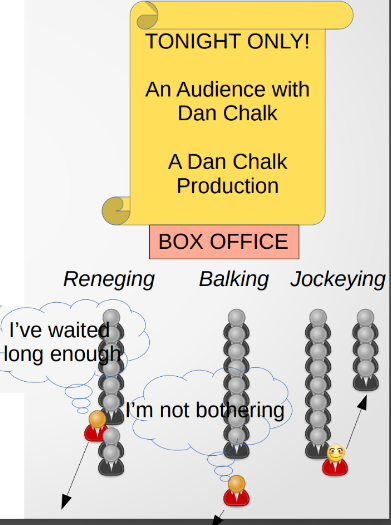
\includegraphics{images/reneging_balking_jockeying_overview.png}

\section{Reneging}\label{reneging}

Let's imagine that each of our patients has a patience level - an amount
of time they're prepared to wait for the nurse.

To model this, we : - Add patience level as an attribute to each
patient, with some way of determining what a patient's patience is -
When we request a resource, we'll tell SimPy to either wait until the
request can be met OR until the patient's patience has expired
(whichever comes first) - We'll then check what happened - did the
patient wait or did they renege? If they waited, we'll proceed as
before. If they reneged, then they won't see the nurse, and we'll record
that they reneged - We'll add the number of patients that reneged to our
outputs from each run, and take the average number of patients who
reneged per run over the trial.

\subsection{Coding a reneging
examaple}\label{coding-a-reneging-examaple}

\subsubsection{The g class}\label{the-g-class-5}

The g class is unchanged.

\subsubsection{The patient class}\label{the-patient-class-5}

In the patient class, we add a patience attribute.

This determines how long the patient is prepared to wait for the nurse.

Here we just randomly sample an integer between 5 and 50 (so the patient
will be prepared to wait for somewhere between 5 and 50 minutes in the
queue), but in a real world application you would probably want to have
a more refined way of allocating patience to patients (e.g basing
probabilities off prior data, or using a non-uniform named
distribution).

You could have different patience levels for different queues, or just a
general patience level. Or even get creative and have a patience level
that decreases the longer they've been in the system if your system has
multiple steps!

If we want to see the effect of this, we can try changing the patience
levels - but you'll need to make the patience levels MUCH higher as this
system is in bad shape (after 3 days patients are waiting on average
over 3 hours\ldots{} and a lot are waiting much longer!)

Maybe try adding another nurse in to get the system under control first!

\begin{Shaded}
\begin{Highlighting}[]
\KeywordTok{class}\NormalTok{ Patient:}
    \KeywordTok{def} \FunctionTok{\_\_init\_\_}\NormalTok{(}\VariableTok{self}\NormalTok{, p\_id):}
        \VariableTok{self}\NormalTok{.}\BuiltInTok{id} \OperatorTok{=}\NormalTok{ p\_id}
        \VariableTok{self}\NormalTok{.q\_time\_nurse }\OperatorTok{=} \DecValTok{0}
        \VariableTok{self}\NormalTok{.priority }\OperatorTok{=}\NormalTok{ random.randint(}\DecValTok{1}\NormalTok{,}\DecValTok{5}\NormalTok{)}

        \VariableTok{self}\NormalTok{.patience\_nurse }\OperatorTok{=}\NormalTok{ random.randint(}\DecValTok{5}\NormalTok{, }\DecValTok{50}\NormalTok{) }\CommentTok{\#\#NEW}
\end{Highlighting}
\end{Shaded}

\subsubsection{The model class}\label{the-model-class-5}

\paragraph{\texorpdfstring{The \textbf{init}
method}{The init method}}\label{the-init-method-2}

In the init method, we set up an additional attribute to track the
number of people reneging.

\begin{Shaded}
\begin{Highlighting}[]
\KeywordTok{def} \FunctionTok{\_\_init\_\_}\NormalTok{(}\VariableTok{self}\NormalTok{, run\_number):}
    \CommentTok{\# Set up SimPy environment}
    \VariableTok{self}\NormalTok{.env }\OperatorTok{=}\NormalTok{ simpy.Environment()}

    \CommentTok{\# Set up counters to use as entity IDs}
    \VariableTok{self}\NormalTok{.patient\_counter }\OperatorTok{=} \DecValTok{0}

    \CommentTok{\# Set up resources}
    \VariableTok{self}\NormalTok{.nurse }\OperatorTok{=}\NormalTok{ simpy.PriorityResource(}\VariableTok{self}\NormalTok{.env,}
\NormalTok{                                        capacity}\OperatorTok{=}\NormalTok{g.number\_of\_nurses)}

    \CommentTok{\# Set run number from value passed in}
    \VariableTok{self}\NormalTok{.run\_number }\OperatorTok{=}\NormalTok{ run\_number}

    \CommentTok{\# Set up DataFrame to store patient{-}level results}
    \VariableTok{self}\NormalTok{.results\_df }\OperatorTok{=}\NormalTok{ pd.DataFrame()}
    \VariableTok{self}\NormalTok{.results\_df[}\StringTok{"Patient ID"}\NormalTok{] }\OperatorTok{=}\NormalTok{ [}\DecValTok{1}\NormalTok{]}
    \VariableTok{self}\NormalTok{.results\_df[}\StringTok{"Q Time Nurse"}\NormalTok{] }\OperatorTok{=}\NormalTok{ [}\FloatTok{0.0}\NormalTok{]}
    \VariableTok{self}\NormalTok{.results\_df.set\_index(}\StringTok{"Patient ID"}\NormalTok{, inplace}\OperatorTok{=}\VariableTok{True}\NormalTok{)}

    \CommentTok{\# Set up attributes that will store mean queuing times across the run}
    \VariableTok{self}\NormalTok{.mean\_q\_time\_nurse }\OperatorTok{=} \DecValTok{0}

    \CommentTok{\#\#NEW {-} we\textquotesingle{}ll set up a new attribute that will store the number of}
    \CommentTok{\# people that reneged from queues in the run (we only have one queue in}
    \CommentTok{\# this model)}
    \VariableTok{self}\NormalTok{.num\_reneged\_nurse }\OperatorTok{=} \DecValTok{0}

\NormalTok{    random.seed(}\DecValTok{42}\NormalTok{)}
\end{Highlighting}
\end{Shaded}

\subsubsection{The attend\_clinic
method}\label{the-attend_clinic-method-3}

In the attend clinic, we now add in an OR statement (the vertical line
\textbar{} , also known as a pipe) to our request for the nurse.

\begin{Shaded}
\begin{Highlighting}[]
\NormalTok{result\_of\_queue }\OperatorTok{=}\NormalTok{ (}\ControlFlowTok{yield}\NormalTok{ req }\OperatorTok{|} \VariableTok{self}\NormalTok{.env.timeout(patient.patience\_nurse))}
\end{Highlighting}
\end{Shaded}

It basically says ``Wait for the request for the nurse to be fulfilled
OR until the patient's patience level has passed, whichever comes first,
and then store whatever the outcome was.

We then need to check whether we got our req - the resource we requested
- or whether the timeout occurred.

We do this with conditional logic:

\begin{Shaded}
\begin{Highlighting}[]
\ControlFlowTok{if}\NormalTok{ req }\KeywordTok{in}\NormalTok{ result\_of\_queue:}
\end{Highlighting}
\end{Shaded}

The indented code after this statement will only take place if the
resource became available before the patient's patience ran out (i.e.~if
the resource became available before the patience period elapsed).

\begin{Shaded}
\begin{Highlighting}[]
\KeywordTok{def}\NormalTok{ attend\_clinic(}\VariableTok{self}\NormalTok{, patient):}
    \CommentTok{\# Nurse consultation activity}
\NormalTok{    start\_q\_nurse }\OperatorTok{=} \VariableTok{self}\NormalTok{.env.now}

    \ControlFlowTok{with} \VariableTok{self}\NormalTok{.nurse.request(priority}\OperatorTok{=}\NormalTok{patient.priority) }\ImportTok{as}\NormalTok{ req:}
        \CommentTok{\#\#NEW}
\NormalTok{        result\_of\_queue }\OperatorTok{=}\NormalTok{ (}\ControlFlowTok{yield}\NormalTok{ req }\OperatorTok{|}
                            \VariableTok{self}\NormalTok{.env.timeout(patient.patience\_nurse))}

        \CommentTok{\#\#NEW {-} we now need to check whether the patient waited or reneged,}
        \CommentTok{\# as we could have got to this point of the generator function}
        \CommentTok{\# either way.  We\textquotesingle{}ll now only get them to see the nurse if they}
        \CommentTok{\# waited.  If they didn\textquotesingle{}t wait, we\textquotesingle{}ll add to our counter of how}
        \CommentTok{\# many patients reneged from the queue.}
        \ControlFlowTok{if}\NormalTok{ req }\KeywordTok{in}\NormalTok{ result\_of\_queue:}
\NormalTok{            end\_q\_nurse }\OperatorTok{=} \VariableTok{self}\NormalTok{.env.now}

\NormalTok{            patient.q\_time\_nurse }\OperatorTok{=}\NormalTok{ end\_q\_nurse }\OperatorTok{{-}}\NormalTok{ start\_q\_nurse}

            \ControlFlowTok{if} \VariableTok{self}\NormalTok{.env.now }\OperatorTok{\textgreater{}}\NormalTok{ g.warm\_up\_period:}
                \VariableTok{self}\NormalTok{.results\_df.at[patient.}\BuiltInTok{id}\NormalTok{, }\StringTok{"Q Time Nurse"}\NormalTok{] }\OperatorTok{=}\NormalTok{ (}
\NormalTok{                    patient.q\_time\_nurse}
\NormalTok{                )}

\NormalTok{            sampled\_nurse\_act\_time }\OperatorTok{=}\NormalTok{ Lognormal(}
\NormalTok{                g.mean\_n\_consult\_time, g.sd\_n\_consult\_time).sample()}

            \ControlFlowTok{yield} \VariableTok{self}\NormalTok{.env.timeout(sampled\_nurse\_act\_time)}
        \ControlFlowTok{else}\NormalTok{:}
            \VariableTok{self}\NormalTok{.num\_reneged\_nurse }\OperatorTok{+=} \DecValTok{1}

            \BuiltInTok{print}\NormalTok{ (}\SpecialStringTok{f"Patient }\SpecialCharTok{\{}\NormalTok{patient}\SpecialCharTok{.}\BuiltInTok{id}\SpecialCharTok{\}}\SpecialStringTok{ reneged after waiting"}\NormalTok{,}
                    \SpecialStringTok{f"}\SpecialCharTok{\{}\NormalTok{patient}\SpecialCharTok{.}\NormalTok{patience\_nurse}\SpecialCharTok{\}}\SpecialStringTok{ minutes"}\NormalTok{)}
\end{Highlighting}
\end{Shaded}

\subsubsection{The run method}\label{the-run-method-4}

The only change to the run method is adding a print statement to the end
of it to print the patients who reneged.

\begin{Shaded}
\begin{Highlighting}[]
\BuiltInTok{print}\NormalTok{ (}\SpecialStringTok{f"}\SpecialCharTok{\{}\VariableTok{self}\SpecialCharTok{.}\NormalTok{num\_reneged\_nurse}\SpecialCharTok{\}}\SpecialStringTok{ patients reneged from nurse queue"}\NormalTok{)}
\end{Highlighting}
\end{Shaded}

\subsubsection{The Trial class}\label{the-trial-class-4}

\paragraph{\texorpdfstring{The \textbf{init}
method}{The init method}}\label{the-init-method-3}

In the init method, we add in an addiitonal attribute that is a
placeholder column for the number of people in each run who reneged.

\begin{Shaded}
\begin{Highlighting}[]
\KeywordTok{def}  \FunctionTok{\_\_init\_\_}\NormalTok{(}\VariableTok{self}\NormalTok{):}
    \VariableTok{self}\NormalTok{.df\_trial\_results }\OperatorTok{=}\NormalTok{ pd.DataFrame()}
    \VariableTok{self}\NormalTok{.df\_trial\_results[}\StringTok{"Run Number"}\NormalTok{] }\OperatorTok{=}\NormalTok{ [}\DecValTok{0}\NormalTok{]}
    \VariableTok{self}\NormalTok{.df\_trial\_results[}\StringTok{"Mean Q Time Nurse"}\NormalTok{] }\OperatorTok{=}\NormalTok{ [}\FloatTok{0.0}\NormalTok{]}
    \CommentTok{\#\#NEW {-} additional column of trial results to store the number of}
    \CommentTok{\# patients that reneged in each run}
    \VariableTok{self}\NormalTok{.df\_trial\_results[}\StringTok{"Reneged Q Nurse"}\NormalTok{] }\OperatorTok{=}\NormalTok{ [}\DecValTok{0}\NormalTok{]}
    \VariableTok{self}\NormalTok{.df\_trial\_results.set\_index(}\StringTok{"Run Number"}\NormalTok{, inplace}\OperatorTok{=}\VariableTok{True}\NormalTok{)}
\end{Highlighting}
\end{Shaded}

\paragraph{The calculate\_means\_over\_trial
method}\label{the-calculate_means_over_trial-method}

We also now need to calculate the mean number of patients reneging per
run.

\begin{Shaded}
\begin{Highlighting}[]
\KeywordTok{def}\NormalTok{ calculate\_means\_over\_trial(}\VariableTok{self}\NormalTok{):}
    \VariableTok{self}\NormalTok{.mean\_q\_time\_nurse\_trial }\OperatorTok{=}\NormalTok{ (}
        \VariableTok{self}\NormalTok{.df\_trial\_results[}\StringTok{"Mean Q Time Nurse"}\NormalTok{].mean()}
\NormalTok{    )}

    \CommentTok{\#\#NEW}
    \VariableTok{self}\NormalTok{.mean\_reneged\_q\_nurse }\OperatorTok{=}\NormalTok{ (}
        \VariableTok{self}\NormalTok{.df\_trial\_results[}\StringTok{"Reneged Q Nurse"}\NormalTok{].mean()}
\NormalTok{    )}
\end{Highlighting}
\end{Shaded}

\paragraph{The print\_trial\_results
method}\label{the-print_trial_results-method}

\begin{Shaded}
\begin{Highlighting}[]
\KeywordTok{def}\NormalTok{ print\_trial\_results(}\VariableTok{self}\NormalTok{):}
    \BuiltInTok{print}\NormalTok{ (}\StringTok{"Trial Results"}\NormalTok{)}
    \BuiltInTok{print}\NormalTok{ (}\VariableTok{self}\NormalTok{.df\_trial\_results)}

    \BuiltInTok{print}\NormalTok{ (}\SpecialStringTok{f"Mean Q Nurse : }\SpecialCharTok{\{}\VariableTok{self}\SpecialCharTok{.}\NormalTok{mean\_q\_time\_nurse\_trial}\SpecialCharTok{:.1f\}}\SpecialStringTok{ minutes"}\NormalTok{)}
    \CommentTok{\#\#NEW {-} we will also now print out the mean number of patients who}
    \CommentTok{\# reneged from the nurse\textquotesingle{}s queue per run}
    \BuiltInTok{print}\NormalTok{ (}\SpecialStringTok{f"Mean Reneged Q Nurse : }\SpecialCharTok{\{}\VariableTok{self}\SpecialCharTok{.}\NormalTok{mean\_reneged\_q\_nurse}\SpecialCharTok{\}}\SpecialStringTok{ patients"}\NormalTok{)}
\end{Highlighting}
\end{Shaded}

\paragraph{The run\_trial method}\label{the-run_trial-method-1}

We also need to add the number of patients who reneged from the nurse's
queue as one of the results against each run.

\begin{Shaded}
\begin{Highlighting}[]
\KeywordTok{def}\NormalTok{ run\_trial(}\VariableTok{self}\NormalTok{):}
    \ControlFlowTok{for}\NormalTok{ run }\KeywordTok{in} \BuiltInTok{range}\NormalTok{(g.number\_of\_runs):}
\NormalTok{        my\_model }\OperatorTok{=}\NormalTok{ Model(run)}
\NormalTok{        my\_model.run()}


        \VariableTok{self}\NormalTok{.df\_trial\_results.loc[run] }\OperatorTok{=}\NormalTok{ [my\_model.mean\_q\_time\_nurse,}
\NormalTok{                                            my\_model.num\_reneged\_nurse] }\CommentTok{\#\#NEW}

    \VariableTok{self}\NormalTok{.calculate\_means\_over\_trial()}
    \VariableTok{self}\NormalTok{.print\_trial\_results()}
\end{Highlighting}
\end{Shaded}

\subsection{The Full Code}\label{the-full-code-4}

\begin{tcolorbox}[enhanced jigsaw, colframe=quarto-callout-note-color-frame, bottomtitle=1mm, breakable, rightrule=.15mm, coltitle=black, colbacktitle=quarto-callout-note-color!10!white, opacityback=0, leftrule=.75mm, arc=.35mm, toptitle=1mm, title=\textcolor{quarto-callout-note-color}{\faInfo}\hspace{0.5em}{Click here to view the full code}, titlerule=0mm, colback=white, toprule=.15mm, bottomrule=.15mm, left=2mm, opacitybacktitle=0.6]

\begin{Shaded}
\begin{Highlighting}[]
\ImportTok{import}\NormalTok{ simpy}
\ImportTok{import}\NormalTok{ random}
\ImportTok{import}\NormalTok{ pandas }\ImportTok{as}\NormalTok{ pd}
\ImportTok{from}\NormalTok{ sim\_tools.distributions }\ImportTok{import}\NormalTok{ Lognormal}


\CommentTok{\# Class to store global parameter values.}
\KeywordTok{class}\NormalTok{ g:}
    \CommentTok{\# Inter{-}arrival times}
\NormalTok{    patient\_inter }\OperatorTok{=} \DecValTok{5}

    \CommentTok{\# Activity times}
\NormalTok{    mean\_n\_consult\_time }\OperatorTok{=} \DecValTok{6}
\NormalTok{    sd\_n\_consult\_time }\OperatorTok{=} \DecValTok{1}

    \CommentTok{\# Resource numbers}
\NormalTok{    number\_of\_nurses }\OperatorTok{=} \DecValTok{1}

    \CommentTok{\# Resource unavailability duration and frequency}
\NormalTok{    unav\_time\_nurse }\OperatorTok{=} \DecValTok{15}
\NormalTok{    unav\_freq\_nurse }\OperatorTok{=} \DecValTok{120}

    \CommentTok{\# Simulation meta parameters}
\NormalTok{    sim\_duration }\OperatorTok{=} \DecValTok{120}
\NormalTok{    number\_of\_runs }\OperatorTok{=} \DecValTok{1}
\NormalTok{    warm\_up\_period }\OperatorTok{=} \DecValTok{360}

\NormalTok{    random.seed(}\DecValTok{42}\NormalTok{)}

\CommentTok{\# Class representing patients coming in to the clinic.}
\KeywordTok{class}\NormalTok{ Patient:}
    \KeywordTok{def} \FunctionTok{\_\_init\_\_}\NormalTok{(}\VariableTok{self}\NormalTok{, p\_id):}
        \VariableTok{self}\NormalTok{.}\BuiltInTok{id} \OperatorTok{=}\NormalTok{ p\_id}
        \VariableTok{self}\NormalTok{.q\_time\_nurse }\OperatorTok{=} \DecValTok{0}
        \VariableTok{self}\NormalTok{.priority }\OperatorTok{=}\NormalTok{ random.randint(}\DecValTok{1}\NormalTok{,}\DecValTok{5}\NormalTok{)}

        \CommentTok{\#\#NEW {-} added a new patience attribute of the patient.  This determines}
        \CommentTok{\# how long the patient is prepared to wait for the nurse.  Here we just}
        \CommentTok{\# randomly sample an integer between 5 and 50 (so the patient will be}
        \CommentTok{\# prepared to wait for somewhere between 5 and 50 minutes in the queue),}
        \CommentTok{\# but in a real world application you would probably want to have a}
        \CommentTok{\# more refined way of allocating patience to patients (e.g basing}
        \CommentTok{\# probabilities off prior data, or using a non{-}uniform named}
        \CommentTok{\# distribution).  You could have different patience levels for different}
        \CommentTok{\# queues, or just a general patience level.  Or even get creative and}
        \CommentTok{\# have a patience level that decreases the longer they\textquotesingle{}ve been in the}
        \CommentTok{\# system!}
        \CommentTok{\# If we want to see the effect of this, we can try changing the patience}
        \CommentTok{\# levels {-} but you\textquotesingle{}ll need to make the patience levels MUCH higher as}
        \CommentTok{\# this system is in bad shape (remember, after 3 days patients are}
        \CommentTok{\# waiting on average over 3 hours... and a lot are waiting much longer!)}
        \CommentTok{\# Maybe try adding another nurse in to get the system under control}
        \CommentTok{\# first!}
        \VariableTok{self}\NormalTok{.patience\_nurse }\OperatorTok{=}\NormalTok{ random.randint(}\DecValTok{5}\NormalTok{, }\DecValTok{50}\NormalTok{)}

\CommentTok{\# Class representing our model of the clinic.}
\KeywordTok{class}\NormalTok{ Model:}
    \CommentTok{\# Constructor}
    \KeywordTok{def} \FunctionTok{\_\_init\_\_}\NormalTok{(}\VariableTok{self}\NormalTok{, run\_number):}
        \CommentTok{\# Set up SimPy environment}
        \VariableTok{self}\NormalTok{.env }\OperatorTok{=}\NormalTok{ simpy.Environment()}

        \CommentTok{\# Set up counters to use as entity IDs}
        \VariableTok{self}\NormalTok{.patient\_counter }\OperatorTok{=} \DecValTok{0}

        \CommentTok{\# Set up resources}
        \VariableTok{self}\NormalTok{.nurse }\OperatorTok{=}\NormalTok{ simpy.PriorityResource(}\VariableTok{self}\NormalTok{.env,}
\NormalTok{                                            capacity}\OperatorTok{=}\NormalTok{g.number\_of\_nurses)}

        \CommentTok{\# Set run number from value passed in}
        \VariableTok{self}\NormalTok{.run\_number }\OperatorTok{=}\NormalTok{ run\_number}

        \CommentTok{\# Set up DataFrame to store patient{-}level results}
        \VariableTok{self}\NormalTok{.results\_df }\OperatorTok{=}\NormalTok{ pd.DataFrame()}
        \VariableTok{self}\NormalTok{.results\_df[}\StringTok{"Patient ID"}\NormalTok{] }\OperatorTok{=}\NormalTok{ [}\DecValTok{1}\NormalTok{]}
        \VariableTok{self}\NormalTok{.results\_df[}\StringTok{"Q Time Nurse"}\NormalTok{] }\OperatorTok{=}\NormalTok{ [}\FloatTok{0.0}\NormalTok{]}
        \VariableTok{self}\NormalTok{.results\_df.set\_index(}\StringTok{"Patient ID"}\NormalTok{, inplace}\OperatorTok{=}\VariableTok{True}\NormalTok{)}

        \CommentTok{\# Set up attributes that will store mean queuing times across the run}
        \VariableTok{self}\NormalTok{.mean\_q\_time\_nurse }\OperatorTok{=} \DecValTok{0}

        \CommentTok{\#\#NEW {-} we\textquotesingle{}ll set up a new attribute that will store the number of}
        \CommentTok{\# people that reneged from queues in the run (we only have one queue in}
        \CommentTok{\# this model)}
        \VariableTok{self}\NormalTok{.num\_reneged\_nurse }\OperatorTok{=} \DecValTok{0}

    \CommentTok{\# Generator function that represents the DES generator for patient arrivals}
    \KeywordTok{def}\NormalTok{ generator\_patient\_arrivals(}\VariableTok{self}\NormalTok{):}
        \ControlFlowTok{while} \VariableTok{True}\NormalTok{:}
            \VariableTok{self}\NormalTok{.patient\_counter }\OperatorTok{+=} \DecValTok{1}

\NormalTok{            p }\OperatorTok{=}\NormalTok{ Patient(}\VariableTok{self}\NormalTok{.patient\_counter)}

            \VariableTok{self}\NormalTok{.env.process(}\VariableTok{self}\NormalTok{.attend\_clinic(p))}

\NormalTok{            sampled\_inter }\OperatorTok{=}\NormalTok{ random.expovariate(}\FloatTok{1.0} \OperatorTok{/}\NormalTok{ g.patient\_inter)}

            \ControlFlowTok{yield} \VariableTok{self}\NormalTok{.env.timeout(sampled\_inter)}


    \CommentTok{\# Generator function representing pathway for patients attending the}
    \CommentTok{\# clinic.}
    \KeywordTok{def}\NormalTok{ attend\_clinic(}\VariableTok{self}\NormalTok{, patient):}
        \CommentTok{\# Nurse consultation activity}
\NormalTok{        start\_q\_nurse }\OperatorTok{=} \VariableTok{self}\NormalTok{.env.now}

        \ControlFlowTok{with} \VariableTok{self}\NormalTok{.nurse.request(priority}\OperatorTok{=}\NormalTok{patient.priority) }\ImportTok{as}\NormalTok{ req:}
            \CommentTok{\#\#NEW {-} this statement now uses a vertical bar (|) / pipe as an "or"}
            \CommentTok{\# statement.  It basically says "Wait for the request for the nurse}
            \CommentTok{\# to be fulfilled OR until the patient\textquotesingle{}s patience level has passed,}
            \CommentTok{\# whichever comes first, and then store whatever the outcome was.}
\NormalTok{            result\_of\_queue }\OperatorTok{=}\NormalTok{ (}\ControlFlowTok{yield}\NormalTok{ req }\OperatorTok{|}
                               \VariableTok{self}\NormalTok{.env.timeout(patient.patience\_nurse))}

            \CommentTok{\#\#NEW {-} we now need to check whether the patient waited or reneged,}
            \CommentTok{\# as we could have got to this point of the generator function}
            \CommentTok{\# either way.  We\textquotesingle{}ll now only get them to see the nurse if they}
            \CommentTok{\# waited.  If they didn\textquotesingle{}t wait, we\textquotesingle{}ll add to our counter of how}
            \CommentTok{\# many patients reneged from the queue.}
            \ControlFlowTok{if}\NormalTok{ req }\KeywordTok{in}\NormalTok{ result\_of\_queue:}
\NormalTok{                end\_q\_nurse }\OperatorTok{=} \VariableTok{self}\NormalTok{.env.now}

\NormalTok{                patient.q\_time\_nurse }\OperatorTok{=}\NormalTok{ end\_q\_nurse }\OperatorTok{{-}}\NormalTok{ start\_q\_nurse}

                \ControlFlowTok{if} \VariableTok{self}\NormalTok{.env.now }\OperatorTok{\textgreater{}}\NormalTok{ g.warm\_up\_period:}
                    \VariableTok{self}\NormalTok{.results\_df.at[patient.}\BuiltInTok{id}\NormalTok{, }\StringTok{"Q Time Nurse"}\NormalTok{] }\OperatorTok{=}\NormalTok{ (}
\NormalTok{                        patient.q\_time\_nurse}
\NormalTok{                    )}

\NormalTok{                sampled\_nurse\_act\_time }\OperatorTok{=}\NormalTok{ Lognormal(}
\NormalTok{                    g.mean\_n\_consult\_time, g.sd\_n\_consult\_time).sample()}

                \ControlFlowTok{yield} \VariableTok{self}\NormalTok{.env.timeout(sampled\_nurse\_act\_time)}
            \ControlFlowTok{else}\NormalTok{:}
                \VariableTok{self}\NormalTok{.num\_reneged\_nurse }\OperatorTok{+=} \DecValTok{1}

                \BuiltInTok{print}\NormalTok{ (}\SpecialStringTok{f"Patient }\SpecialCharTok{\{}\NormalTok{patient}\SpecialCharTok{.}\BuiltInTok{id}\SpecialCharTok{\}}\SpecialStringTok{ reneged after waiting"}\NormalTok{,}
                       \SpecialStringTok{f"}\SpecialCharTok{\{}\NormalTok{patient}\SpecialCharTok{.}\NormalTok{patience\_nurse}\SpecialCharTok{\}}\SpecialStringTok{ minutes"}\NormalTok{)}

    \CommentTok{\# Method to calculate and store results over the run}
    \KeywordTok{def}\NormalTok{ calculate\_run\_results(}\VariableTok{self}\NormalTok{):}
        \VariableTok{self}\NormalTok{.results\_df.drop([}\DecValTok{1}\NormalTok{], inplace}\OperatorTok{=}\VariableTok{True}\NormalTok{)}

        \VariableTok{self}\NormalTok{.mean\_q\_time\_nurse }\OperatorTok{=} \VariableTok{self}\NormalTok{.results\_df[}\StringTok{"Q Time Nurse"}\NormalTok{].mean()}

    \CommentTok{\# Method to run a single run of the simulation}
    \KeywordTok{def}\NormalTok{ run(}\VariableTok{self}\NormalTok{):}
        \CommentTok{\# Start up DES generators}
        \VariableTok{self}\NormalTok{.env.process(}\VariableTok{self}\NormalTok{.generator\_patient\_arrivals())}

        \CommentTok{\# Run for the duration specified in g class}
        \VariableTok{self}\NormalTok{.env.run(until}\OperatorTok{=}\NormalTok{(g.sim\_duration }\OperatorTok{+}\NormalTok{ g.warm\_up\_period))}

        \CommentTok{\# Calculate results over the run}
        \VariableTok{self}\NormalTok{.calculate\_run\_results()}

        \CommentTok{\# Print patient level results for this run}
        \BuiltInTok{print}\NormalTok{ (}\SpecialStringTok{f"Run Number }\SpecialCharTok{\{}\VariableTok{self}\SpecialCharTok{.}\NormalTok{run\_number}\SpecialCharTok{\}}\SpecialStringTok{"}\NormalTok{)}
        \BuiltInTok{print}\NormalTok{ (}\VariableTok{self}\NormalTok{.results\_df)}
        \CommentTok{\#\#NEW {-} we\textquotesingle{}ll print out the number of patients that reneged from the}
        \CommentTok{\# nurse queue in this run of the model.}
        \BuiltInTok{print}\NormalTok{ (}\SpecialStringTok{f"}\SpecialCharTok{\{}\VariableTok{self}\SpecialCharTok{.}\NormalTok{num\_reneged\_nurse}\SpecialCharTok{\}}\SpecialStringTok{ patients reneged from nurse queue"}\NormalTok{)}

\CommentTok{\# Class representing a Trial for our simulation}
\KeywordTok{class}\NormalTok{ Trial:}
    \CommentTok{\# Constructor}
    \KeywordTok{def}  \FunctionTok{\_\_init\_\_}\NormalTok{(}\VariableTok{self}\NormalTok{):}
        \VariableTok{self}\NormalTok{.df\_trial\_results }\OperatorTok{=}\NormalTok{ pd.DataFrame()}
        \VariableTok{self}\NormalTok{.df\_trial\_results[}\StringTok{"Run Number"}\NormalTok{] }\OperatorTok{=}\NormalTok{ [}\DecValTok{0}\NormalTok{]}
        \VariableTok{self}\NormalTok{.df\_trial\_results[}\StringTok{"Mean Q Time Nurse"}\NormalTok{] }\OperatorTok{=}\NormalTok{ [}\FloatTok{0.0}\NormalTok{]}
        \CommentTok{\#\#NEW {-} additional column of trial results to store the number of}
        \CommentTok{\# patients that reneged in each run}
        \VariableTok{self}\NormalTok{.df\_trial\_results[}\StringTok{"Reneged Q Nurse"}\NormalTok{] }\OperatorTok{=}\NormalTok{ [}\DecValTok{0}\NormalTok{]}
        \VariableTok{self}\NormalTok{.df\_trial\_results.set\_index(}\StringTok{"Run Number"}\NormalTok{, inplace}\OperatorTok{=}\VariableTok{True}\NormalTok{)}

    \CommentTok{\# Method to calculate and store means across runs in the trial}
    \KeywordTok{def}\NormalTok{ calculate\_means\_over\_trial(}\VariableTok{self}\NormalTok{):}
        \VariableTok{self}\NormalTok{.mean\_q\_time\_nurse\_trial }\OperatorTok{=}\NormalTok{ (}
            \VariableTok{self}\NormalTok{.df\_trial\_results[}\StringTok{"Mean Q Time Nurse"}\NormalTok{].mean()}
\NormalTok{        )}

        \CommentTok{\#\#NEW {-} we also now need to calculate the mean number of patients}
        \CommentTok{\# reneging per run}
        \VariableTok{self}\NormalTok{.mean\_reneged\_q\_nurse }\OperatorTok{=}\NormalTok{ (}
            \VariableTok{self}\NormalTok{.df\_trial\_results[}\StringTok{"Reneged Q Nurse"}\NormalTok{].mean()}
\NormalTok{        )}

    \CommentTok{\# Method to print trial results, including averages across runs}
    \KeywordTok{def}\NormalTok{ print\_trial\_results(}\VariableTok{self}\NormalTok{):}
        \BuiltInTok{print}\NormalTok{ (}\StringTok{"Trial Results"}\NormalTok{)}
        \BuiltInTok{print}\NormalTok{ (}\VariableTok{self}\NormalTok{.df\_trial\_results)}

        \BuiltInTok{print}\NormalTok{ (}\SpecialStringTok{f"Mean Q Nurse : }\SpecialCharTok{\{}\VariableTok{self}\SpecialCharTok{.}\NormalTok{mean\_q\_time\_nurse\_trial}\SpecialCharTok{:.1f\}}\SpecialStringTok{ minutes"}\NormalTok{)}
        \CommentTok{\#\#NEW {-} we will also now print out the mean number of patients who}
        \CommentTok{\# reneged from the nurse\textquotesingle{}s queue per run}
        \BuiltInTok{print}\NormalTok{ (}\SpecialStringTok{f"Mean Reneged Q Nurse : }\SpecialCharTok{\{}\VariableTok{self}\SpecialCharTok{.}\NormalTok{mean\_reneged\_q\_nurse}\SpecialCharTok{\}}\SpecialStringTok{ patients"}\NormalTok{)}

    \CommentTok{\# Method to run trial}
    \KeywordTok{def}\NormalTok{ run\_trial(}\VariableTok{self}\NormalTok{):}
        \ControlFlowTok{for}\NormalTok{ run }\KeywordTok{in} \BuiltInTok{range}\NormalTok{(g.number\_of\_runs):}
\NormalTok{            my\_model }\OperatorTok{=}\NormalTok{ Model(run)}
\NormalTok{            my\_model.run()}

            \CommentTok{\#\#NEW {-} we also need to add the number of patients who reneged from}
            \CommentTok{\# the nurse\textquotesingle{}s queue as one of the results against each run}
            \VariableTok{self}\NormalTok{.df\_trial\_results.loc[run] }\OperatorTok{=}\NormalTok{ [my\_model.mean\_q\_time\_nurse,}
\NormalTok{                                              my\_model.num\_reneged\_nurse]}

        \VariableTok{self}\NormalTok{.calculate\_means\_over\_trial()}
        \VariableTok{self}\NormalTok{.print\_trial\_results()}
\end{Highlighting}
\end{Shaded}

\end{tcolorbox}

\subsection{Exploring the outputs}\label{exploring-the-outputs}

What are the outputs?

\begin{Shaded}
\begin{Highlighting}[]
\CommentTok{\# Create new instance of Trial and run it}
\NormalTok{my\_trial }\OperatorTok{=}\NormalTok{ Trial()}
\NormalTok{my\_trial.run\_trial()}
\end{Highlighting}
\end{Shaded}

\begin{verbatim}
Patient 9 reneged after waiting 22 minutes
Patient 12 reneged after waiting 11 minutes
Patient 17 reneged after waiting 28 minutes
Patient 21 reneged after waiting 15 minutes
Patient 41 reneged after waiting 5 minutes
Patient 35 reneged after waiting 28 minutes
Patient 40 reneged after waiting 38 minutes
Patient 51 reneged after waiting 6 minutes
Patient 61 reneged after waiting 12 minutes
Patient 56 reneged after waiting 40 minutes
Patient 57 reneged after waiting 43 minutes
Patient 63 reneged after waiting 19 minutes
Patient 67 reneged after waiting 22 minutes
Patient 75 reneged after waiting 11 minutes
Patient 80 reneged after waiting 5 minutes
Patient 78 reneged after waiting 9 minutes
Patient 70 reneged after waiting 31 minutes
Patient 79 reneged after waiting 11 minutes
Patient 72 reneged after waiting 31 minutes
Patient 77 reneged after waiting 16 minutes
Patient 92 reneged after waiting 10 minutes
Patient 91 reneged after waiting 15 minutes
Patient 95 reneged after waiting 20 minutes
Patient 90 reneged after waiting 35 minutes
Patient 101 reneged after waiting 25 minutes
Patient 97 reneged after waiting 41 minutes
Run Number 0
            Q Time Nurse
Patient ID              
76             12.656851
69             40.323190
81              1.634667
82              8.502884
83              4.555252
84              8.463305
85              1.595772
86              3.986689
88              3.219940
89              0.769129
87             16.175202
93              1.050912
96              3.718465
94             14.679519
100             3.921112
98             16.589564
99             17.328147
102             2.712001
104             5.358260
26 patients reneged from nurse queue
Trial Results
            Mean Q Time Nurse  Reneged Q Nurse
Run Number                                    
0                    8.802151               26
Mean Q Nurse : 8.8 minutes
Mean Reneged Q Nurse : 26.0 patients
\end{verbatim}

We can see that not every patient is reneging.

We can also see that some patients who arrived in the system later balk
earlier than patients who have been there longer (i.e.~a patient with a
later ID balks before a patient with an earlier ID). This is due to the
randomly set reneging threshold for each patient - some people aren't
willing to wait as long.

\section{Balking}\label{balking}

For balking, there are two different ways in which balking can occur
(and both could occur in the same model) :

\begin{itemize}
\tightlist
\item
  An entity may choose not to join a queue because it is too long for
  their preferences / needs
\item
  An entity may not be able to join a queue because there is no capacity
  for them
\end{itemize}

We will look at the latter, but the way we approach it is the same for
both - the only difference is that, in the former, the maximum queue
length is likely to be an attribute of the patient (and may be
individual per patient) just like in the reneging example, rather than
an attribute of the model.

Here, we'll imagine that in our clinic, there is only space for 3 people
to wait to see the nurse, and if there is no space, they cannot wait.

To model our balking requirements, we will : - Add a parameter to g
class to store the maximum queue length allowed (if this were
patient-decided balking, we'd put this in the patient class instead) -
Add a list to our model attributes that will store all the patient
objects currently in the queue for the nurse. This is really useful as
it allows us to see who is in the queue at any time, as well as how many
etc - Whenever a patient joins or leaves the queue, we'll update the
list of patients in the queue - Before we ask for the nurse resource,
we'll first check if the queue is at maximum size. If it is, the patient
will never join the queue and we'll record that. If not, we'll proceed
as before. We'll add results of number of patients who balked to our
results

\subsection{Coding a balking example}\label{coding-a-balking-example}

\subsubsection{The g Class}\label{the-g-class-6}

We'll add a parameter value that will store the maximum length of the
queue we allow for the nurse.

Let's imagine there's only space for 3 people in the waiting room and so
no more than 3 people can wait at any time.

\begin{tcolorbox}[enhanced jigsaw, colframe=quarto-callout-note-color-frame, bottomtitle=1mm, breakable, rightrule=.15mm, coltitle=black, colbacktitle=quarto-callout-note-color!10!white, opacityback=0, leftrule=.75mm, arc=.35mm, toptitle=1mm, title=\textcolor{quarto-callout-note-color}{\faInfo}\hspace{0.5em}{Note}, titlerule=0mm, colback=white, toprule=.15mm, bottomrule=.15mm, left=2mm, opacitybacktitle=0.6]

Note - we could simulate balking from the perspective of the patient
instead (or as well) - e.g.~the patient will only wait if there are no
more than x people waiting etc. If we did this, we'd probably want to
make this level an attribute of the patient, as it may vary between
patients.

\end{tcolorbox}

\begin{Shaded}
\begin{Highlighting}[]
\KeywordTok{class}\NormalTok{ g:}
    \CommentTok{\# Inter{-}arrival times}
\NormalTok{    patient\_inter }\OperatorTok{=} \DecValTok{5}

    \CommentTok{\# Activity times}
\NormalTok{    mean\_n\_consult\_time }\OperatorTok{=} \DecValTok{6}
\NormalTok{    sd\_n\_consult\_time }\OperatorTok{=} \DecValTok{1}

    \CommentTok{\# Resource numbers}
\NormalTok{    number\_of\_nurses }\OperatorTok{=} \DecValTok{1}

    \CommentTok{\# Resource unavailability duration and frequency}
\NormalTok{    unav\_time\_nurse }\OperatorTok{=} \DecValTok{15}
\NormalTok{    unav\_freq\_nurse }\OperatorTok{=} \DecValTok{120}

    \CommentTok{\#\#NEW}
\NormalTok{    max\_q\_nurse }\OperatorTok{=} \DecValTok{3}

    \CommentTok{\# Simulation meta parameters}
\NormalTok{    sim\_duration }\OperatorTok{=} \DecValTok{2880}
\NormalTok{    number\_of\_runs }\OperatorTok{=} \DecValTok{100}
\NormalTok{    warm\_up\_period }\OperatorTok{=} \DecValTok{1440}
\end{Highlighting}
\end{Shaded}

\subsubsection{The Patient Class}\label{the-patient-class-6}

This class is unchanged.

\subsubsection{The Model Class}\label{the-model-class-6}

\paragraph{\texorpdfstring{The \textbf{init}
method}{The init method}}\label{the-init-method-4}

Here we add in an additional attribute to count the number of people who
balk.

We also we add a list that will store patient objects queuing for the
nurse consultation. This will allow us to see who is in the queue at any
time, as well as the length of the queue etc.

\begin{Shaded}
\begin{Highlighting}[]
\KeywordTok{class}\NormalTok{ Model:}
    \CommentTok{\# Constructor}
    \KeywordTok{def} \FunctionTok{\_\_init\_\_}\NormalTok{(}\VariableTok{self}\NormalTok{, run\_number):}
        \CommentTok{\# Set up SimPy environment}
        \VariableTok{self}\NormalTok{.env }\OperatorTok{=}\NormalTok{ simpy.Environment()}

        \CommentTok{\# Set up counters to use as entity IDs}
        \VariableTok{self}\NormalTok{.patient\_counter }\OperatorTok{=} \DecValTok{0}

        \CommentTok{\# Set up resources}
        \VariableTok{self}\NormalTok{.nurse }\OperatorTok{=}\NormalTok{ simpy.PriorityResource(}\VariableTok{self}\NormalTok{.env,}
\NormalTok{                                            capacity}\OperatorTok{=}\NormalTok{g.number\_of\_nurses)}

        \CommentTok{\# Set run number from value passed in}
        \VariableTok{self}\NormalTok{.run\_number }\OperatorTok{=}\NormalTok{ run\_number}

        \CommentTok{\# Set up DataFrame to store patient{-}level results}
        \VariableTok{self}\NormalTok{.results\_df }\OperatorTok{=}\NormalTok{ pd.DataFrame()}
        \VariableTok{self}\NormalTok{.results\_df[}\StringTok{"Patient ID"}\NormalTok{] }\OperatorTok{=}\NormalTok{ [}\DecValTok{1}\NormalTok{]}
        \VariableTok{self}\NormalTok{.results\_df[}\StringTok{"Q Time Nurse"}\NormalTok{] }\OperatorTok{=}\NormalTok{ [}\FloatTok{0.0}\NormalTok{]}
        \VariableTok{self}\NormalTok{.results\_df.set\_index(}\StringTok{"Patient ID"}\NormalTok{, inplace}\OperatorTok{=}\VariableTok{True}\NormalTok{)}

        \CommentTok{\# Set up attributes that will store mean queuing times across the run}
        \VariableTok{self}\NormalTok{.mean\_q\_time\_nurse }\OperatorTok{=} \DecValTok{0}

        \CommentTok{\# Set up attributes that will store queuing behaviour results across}
        \CommentTok{\# run}
        \VariableTok{self}\NormalTok{.num\_balked\_nurse }\OperatorTok{=} \DecValTok{0} \CommentTok{\#\#NEW}

        \VariableTok{self}\NormalTok{.q\_for\_nurse\_consult }\OperatorTok{=}\NormalTok{ [] }\CommentTok{\#\#NEW}
\end{Highlighting}
\end{Shaded}

\paragraph{The generator\_patient\_arrival
method}\label{the-generator_patient_arrival-method}

This method is unchanged.

\paragraph{The attend\_clinic method}\label{the-attend_clinic-method-4}

\begin{Shaded}
\begin{Highlighting}[]
\KeywordTok{def}\NormalTok{ attend\_clinic(}\VariableTok{self}\NormalTok{, patient):}
        \CommentTok{\#\#NEW {-} we now first check whether there is room for the patient to}
        \CommentTok{\# wait.  If there is, then proceed as before.  If not, then the patient}
        \CommentTok{\# never joins the queue, and we record that a patient balked.}
        \ControlFlowTok{if} \BuiltInTok{len}\NormalTok{(}\VariableTok{self}\NormalTok{.q\_for\_nurse\_consult) }\OperatorTok{\textless{}}\NormalTok{ g.max\_q\_nurse:}
            \CommentTok{\# Nurse consultation activity}
\NormalTok{            start\_q\_nurse }\OperatorTok{=} \VariableTok{self}\NormalTok{.env.now}

            \CommentTok{\#\#NEW {-} add the patient object to the list of patients queuing for}
            \CommentTok{\# the nurse}
            \VariableTok{self}\NormalTok{.q\_for\_nurse\_consult.append(patient)}

            \ControlFlowTok{with} \VariableTok{self}\NormalTok{.nurse.request(priority}\OperatorTok{=}\NormalTok{patient.priority) }\ImportTok{as}\NormalTok{ req:}
                \ControlFlowTok{yield}\NormalTok{ req}

                \CommentTok{\#\#NEW {-} remove the patient object from the list of patients}
                \CommentTok{\# queuing for the nurse (by putting it here, the patient will}
                \CommentTok{\# be removed whether they waited or reneged)}
                \VariableTok{self}\NormalTok{.q\_for\_nurse\_consult.remove(patient)}

\NormalTok{                end\_q\_nurse }\OperatorTok{=} \VariableTok{self}\NormalTok{.env.now}

\NormalTok{                patient.q\_time\_nurse }\OperatorTok{=}\NormalTok{ end\_q\_nurse }\OperatorTok{{-}}\NormalTok{ start\_q\_nurse}

                \ControlFlowTok{if} \VariableTok{self}\NormalTok{.env.now }\OperatorTok{\textgreater{}}\NormalTok{ g.warm\_up\_period:}
                    \VariableTok{self}\NormalTok{.results\_df.at[patient.}\BuiltInTok{id}\NormalTok{, }\StringTok{"Q Time Nurse"}\NormalTok{] }\OperatorTok{=}\NormalTok{ (}
\NormalTok{                        patient.q\_time\_nurse}
\NormalTok{                    )}

\NormalTok{                sampled\_nurse\_act\_time }\OperatorTok{=}\NormalTok{ Lognormal(}
\NormalTok{                    g.mean\_n\_consult\_time, g.sd\_n\_consult\_time).sample()}

                \ControlFlowTok{yield} \VariableTok{self}\NormalTok{.env.timeout(sampled\_nurse\_act\_time)}

        \ControlFlowTok{else}\NormalTok{:}
            \VariableTok{self}\NormalTok{.num\_balked\_nurse }\OperatorTok{+=} \DecValTok{1}
\end{Highlighting}
\end{Shaded}

\paragraph{The calculate\_run\_results
method}\label{the-calculate_run_results-method-3}

This method is unchanged.

\paragraph{The run method}\label{the-run-method-5}

Here we have added a print message displaying how many patients balked
in this run.

\begin{Shaded}
\begin{Highlighting}[]
\KeywordTok{def}\NormalTok{ run(}\VariableTok{self}\NormalTok{):}
    \CommentTok{\# Start up DES generators}
    \VariableTok{self}\NormalTok{.env.process(}\VariableTok{self}\NormalTok{.generator\_patient\_arrivals())}

    \CommentTok{\# Run for the duration specified in g class}
    \VariableTok{self}\NormalTok{.env.run(until}\OperatorTok{=}\NormalTok{(g.sim\_duration }\OperatorTok{+}\NormalTok{ g.warm\_up\_period))}

    \CommentTok{\# Calculate results over the run}
    \VariableTok{self}\NormalTok{.calculate\_run\_results()}

    \CommentTok{\# Print patient level results for this run}
    \BuiltInTok{print}\NormalTok{ (}\SpecialStringTok{f"Run Number }\SpecialCharTok{\{}\VariableTok{self}\SpecialCharTok{.}\NormalTok{run\_number}\SpecialCharTok{\}}\SpecialStringTok{"}\NormalTok{)}
    \BuiltInTok{print}\NormalTok{ (}\VariableTok{self}\NormalTok{.results\_df)}
    \BuiltInTok{print}\NormalTok{ (}\SpecialStringTok{f"}\SpecialCharTok{\{}\VariableTok{self}\SpecialCharTok{.}\NormalTok{num\_balked\_nurse}\SpecialCharTok{\}}\SpecialStringTok{ patients balked at the nurse queue"}\NormalTok{) }\CommentTok{\#\# NEW}
\end{Highlighting}
\end{Shaded}

\subsubsection{The Trial Class}\label{the-trial-class-5}

\paragraph{\texorpdfstring{The \textbf{init}
method}{The init method}}\label{the-init-method-5}

First we add in a column to store the number who balked at the nurse
queue in each run.

\begin{Shaded}
\begin{Highlighting}[]
\KeywordTok{def}  \FunctionTok{\_\_init\_\_}\NormalTok{(}\VariableTok{self}\NormalTok{):}
    \VariableTok{self}\NormalTok{.df\_trial\_results }\OperatorTok{=}\NormalTok{ pd.DataFrame()}
    \VariableTok{self}\NormalTok{.df\_trial\_results[}\StringTok{"Run Number"}\NormalTok{] }\OperatorTok{=}\NormalTok{ [}\DecValTok{0}\NormalTok{]}
    \VariableTok{self}\NormalTok{.df\_trial\_results[}\StringTok{"Mean Q Time Nurse"}\NormalTok{] }\OperatorTok{=}\NormalTok{ [}\FloatTok{0.0}\NormalTok{]}
    \VariableTok{self}\NormalTok{.df\_trial\_results[}\StringTok{"Balked Q Nurse"}\NormalTok{] }\OperatorTok{=}\NormalTok{ [}\DecValTok{0}\NormalTok{] }\CommentTok{\#\#NEW}
    \VariableTok{self}\NormalTok{.df\_trial\_results.set\_index(}\StringTok{"Run Number"}\NormalTok{, inplace}\OperatorTok{=}\VariableTok{True}\NormalTok{)}
\end{Highlighting}
\end{Shaded}

\paragraph{The calculate\_means\_over\_trial
method}\label{the-calculate_means_over_trial-method-1}

We add a calculation of mean number of patients who balked at the nurse
queue per run.

\begin{Shaded}
\begin{Highlighting}[]
    \KeywordTok{def}\NormalTok{ calculate\_means\_over\_trial(}\VariableTok{self}\NormalTok{):}
        \VariableTok{self}\NormalTok{.mean\_q\_time\_nurse\_trial }\OperatorTok{=}\NormalTok{ (}
            \VariableTok{self}\NormalTok{.df\_trial\_results[}\StringTok{"Mean Q Time Nurse"}\NormalTok{].mean()}
\NormalTok{        )}

        \CommentTok{\#\#NEW}
        \VariableTok{self}\NormalTok{.mean\_balked\_q\_nurse }\OperatorTok{=}\NormalTok{ (}
            \VariableTok{self}\NormalTok{.df\_trial\_results[}\StringTok{"Balked Q Nurse"}\NormalTok{].mean()}
\NormalTok{        )}
\end{Highlighting}
\end{Shaded}

\paragraph{The print\_trial\_results
method}\label{the-print_trial_results-method-1}

We add in a print message of mean number of patients balking at nurse
queue per run.

\begin{Shaded}
\begin{Highlighting}[]
\KeywordTok{def}\NormalTok{ print\_trial\_results(}\VariableTok{self}\NormalTok{):}
    \BuiltInTok{print}\NormalTok{ (}\StringTok{"Trial Results"}\NormalTok{)}
    \BuiltInTok{print}\NormalTok{ (}\VariableTok{self}\NormalTok{.df\_trial\_results)}

    \BuiltInTok{print}\NormalTok{ (}\SpecialStringTok{f"Mean Q Nurse : }\SpecialCharTok{\{}\VariableTok{self}\SpecialCharTok{.}\NormalTok{mean\_q\_time\_nurse\_trial}\SpecialCharTok{:.1f\}}\SpecialStringTok{ minutes"}\NormalTok{)}

    \BuiltInTok{print}\NormalTok{ (}\SpecialStringTok{f"Mean Balked Q Nurse : }\SpecialCharTok{\{}\VariableTok{self}\SpecialCharTok{.}\NormalTok{mean\_balked\_q\_nurse}\SpecialCharTok{\}}\SpecialStringTok{ patients"}\NormalTok{) }\CommentTok{\#\#NEW}
\end{Highlighting}
\end{Shaded}

\paragraph{The run\_trial method}\label{the-run_trial-method-2}

Finally we add the number that balked at the nurse queue to results in
the run.

\begin{Shaded}
\begin{Highlighting}[]
\KeywordTok{def}\NormalTok{ run\_trial(}\VariableTok{self}\NormalTok{):}
    \ControlFlowTok{for}\NormalTok{ run }\KeywordTok{in} \BuiltInTok{range}\NormalTok{(g.number\_of\_runs):}
\NormalTok{        my\_model }\OperatorTok{=}\NormalTok{ Model(run)}
\NormalTok{        my\_model.run()}

        \VariableTok{self}\NormalTok{.df\_trial\_results.loc[run] }\OperatorTok{=}\NormalTok{ [my\_model.mean\_q\_time\_nurse,}
\NormalTok{                                            my\_model.num\_balked\_nurse] }\CommentTok{\#\#NEW}

    \VariableTok{self}\NormalTok{.calculate\_means\_over\_trial()}
    \VariableTok{self}\NormalTok{.print\_trial\_results()}
\end{Highlighting}
\end{Shaded}

\subsection{The full code}\label{the-full-code-5}

The full code can be seen below:

\begin{tcolorbox}[enhanced jigsaw, colframe=quarto-callout-note-color-frame, bottomtitle=1mm, breakable, rightrule=.15mm, coltitle=black, colbacktitle=quarto-callout-note-color!10!white, opacityback=0, leftrule=.75mm, arc=.35mm, toptitle=1mm, title=\textcolor{quarto-callout-note-color}{\faInfo}\hspace{0.5em}{Click here to view the full code}, titlerule=0mm, colback=white, toprule=.15mm, bottomrule=.15mm, left=2mm, opacitybacktitle=0.6]

\begin{Shaded}
\begin{Highlighting}[]
\ImportTok{import}\NormalTok{ simpy}
\ImportTok{import}\NormalTok{ random}
\ImportTok{import}\NormalTok{ pandas }\ImportTok{as}\NormalTok{ pd}
\ImportTok{from}\NormalTok{ sim\_tools.distributions }\ImportTok{import}\NormalTok{ Lognormal}

\CommentTok{\# Class to store global parameter values.}
\KeywordTok{class}\NormalTok{ g:}
    \CommentTok{\# Inter{-}arrival times}
\NormalTok{    patient\_inter }\OperatorTok{=} \DecValTok{5}

    \CommentTok{\# Activity times}
\NormalTok{    mean\_n\_consult\_time }\OperatorTok{=} \DecValTok{6}
\NormalTok{    sd\_n\_consult\_time }\OperatorTok{=} \DecValTok{1}

    \CommentTok{\# Resource numbers}
\NormalTok{    number\_of\_nurses }\OperatorTok{=} \DecValTok{1}

    \CommentTok{\#\#NEW {-} we\textquotesingle{}ll add a parameter value that will store the maximum length of}
    \CommentTok{\# the queue we allow for the nurse.  Let\textquotesingle{}s imagine there\textquotesingle{}s only space for 3}
    \CommentTok{\# people in the waiting room and so no more than 3 people can wait at any}
    \CommentTok{\# time.  Note {-} we could simulate balking from the perspective of the}
    \CommentTok{\# patient instead (or as well) {-} e.g. the patient will only wait if there}
    \CommentTok{\# are no more than x people waiting etc.  If we did this, we\textquotesingle{}d probably}
    \CommentTok{\# want to make this level an attribute of the patient, as it may vary}
    \CommentTok{\# between patients.}
\NormalTok{    max\_q\_nurse }\OperatorTok{=} \DecValTok{3}

    \CommentTok{\# Simulation meta parameters}
\NormalTok{    sim\_duration }\OperatorTok{=} \DecValTok{2880}
\NormalTok{    number\_of\_runs }\OperatorTok{=} \DecValTok{3}
\NormalTok{    warm\_up\_period }\OperatorTok{=} \DecValTok{1440}

\CommentTok{\# Class representing patients coming in to the clinic.}
\KeywordTok{class}\NormalTok{ Patient:}
    \KeywordTok{def} \FunctionTok{\_\_init\_\_}\NormalTok{(}\VariableTok{self}\NormalTok{, p\_id):}
        \VariableTok{self}\NormalTok{.}\BuiltInTok{id} \OperatorTok{=}\NormalTok{ p\_id}
        \VariableTok{self}\NormalTok{.q\_time\_nurse }\OperatorTok{=} \DecValTok{0}
        \VariableTok{self}\NormalTok{.priority }\OperatorTok{=}\NormalTok{ random.randint(}\DecValTok{1}\NormalTok{,}\DecValTok{5}\NormalTok{)}
        \VariableTok{self}\NormalTok{.patience\_nurse }\OperatorTok{=}\NormalTok{ random.randint(}\DecValTok{5}\NormalTok{, }\DecValTok{50}\NormalTok{)}

\CommentTok{\# Class representing our model of the clinic.}
\KeywordTok{class}\NormalTok{ Model:}
    \CommentTok{\# Constructor}
    \KeywordTok{def} \FunctionTok{\_\_init\_\_}\NormalTok{(}\VariableTok{self}\NormalTok{, run\_number):}
        \CommentTok{\# Set up SimPy environment}
        \VariableTok{self}\NormalTok{.env }\OperatorTok{=}\NormalTok{ simpy.Environment()}

        \CommentTok{\# Set up counters to use as entity IDs}
        \VariableTok{self}\NormalTok{.patient\_counter }\OperatorTok{=} \DecValTok{0}

        \CommentTok{\# Set up resources}
        \VariableTok{self}\NormalTok{.nurse }\OperatorTok{=}\NormalTok{ simpy.PriorityResource(}\VariableTok{self}\NormalTok{.env,}
\NormalTok{                                            capacity}\OperatorTok{=}\NormalTok{g.number\_of\_nurses)}

        \CommentTok{\# Set run number from value passed in}
        \VariableTok{self}\NormalTok{.run\_number }\OperatorTok{=}\NormalTok{ run\_number}

        \CommentTok{\# Set up DataFrame to store patient{-}level results}
        \VariableTok{self}\NormalTok{.results\_df }\OperatorTok{=}\NormalTok{ pd.DataFrame()}
        \VariableTok{self}\NormalTok{.results\_df[}\StringTok{"Patient ID"}\NormalTok{] }\OperatorTok{=}\NormalTok{ [}\DecValTok{1}\NormalTok{]}
        \VariableTok{self}\NormalTok{.results\_df[}\StringTok{"Q Time Nurse"}\NormalTok{] }\OperatorTok{=}\NormalTok{ [}\FloatTok{0.0}\NormalTok{]}
        \VariableTok{self}\NormalTok{.results\_df.set\_index(}\StringTok{"Patient ID"}\NormalTok{, inplace}\OperatorTok{=}\VariableTok{True}\NormalTok{)}

        \CommentTok{\# Set up attributes that will store mean queuing times across the run}
        \VariableTok{self}\NormalTok{.mean\_q\_time\_nurse }\OperatorTok{=} \DecValTok{0}

        \CommentTok{\# Set up attributes that will store queuing behaviour results across}
        \CommentTok{\# run}
        \VariableTok{self}\NormalTok{.num\_balked\_nurse }\OperatorTok{=} \DecValTok{0} \CommentTok{\#\#NEW {-} added to record number balking}

        \CommentTok{\#\#NEW {-} we add a list that will store patient objects queuing for the}
        \CommentTok{\# nurse consultation.  This will allow us to see who is in the queue at}
        \CommentTok{\# any time, as well as the length of the queue etc}
        \VariableTok{self}\NormalTok{.q\_for\_nurse\_consult }\OperatorTok{=}\NormalTok{ []}

    \CommentTok{\# Generator function that represents the DES generator for patient arrivals}
    \KeywordTok{def}\NormalTok{ generator\_patient\_arrivals(}\VariableTok{self}\NormalTok{):}
        \ControlFlowTok{while} \VariableTok{True}\NormalTok{:}
            \VariableTok{self}\NormalTok{.patient\_counter }\OperatorTok{+=} \DecValTok{1}

\NormalTok{            p }\OperatorTok{=}\NormalTok{ Patient(}\VariableTok{self}\NormalTok{.patient\_counter)}

            \VariableTok{self}\NormalTok{.env.process(}\VariableTok{self}\NormalTok{.attend\_clinic(p))}

\NormalTok{            sampled\_inter }\OperatorTok{=}\NormalTok{ random.expovariate(}\FloatTok{1.0} \OperatorTok{/}\NormalTok{ g.patient\_inter)}

            \ControlFlowTok{yield} \VariableTok{self}\NormalTok{.env.timeout(sampled\_inter)}

    \CommentTok{\# Generator function representing pathway for patients attending the}
    \CommentTok{\# clinic.}
    \KeywordTok{def}\NormalTok{ attend\_clinic(}\VariableTok{self}\NormalTok{, patient):}
        \CommentTok{\#\#NEW {-} we now first check whether there is room for the patient to}
        \CommentTok{\# wait.  If there is, then proceed as before.  If not, then the patient}
        \CommentTok{\# never joins the queue, and we record that a patient balked.}
        \ControlFlowTok{if} \BuiltInTok{len}\NormalTok{(}\VariableTok{self}\NormalTok{.q\_for\_nurse\_consult) }\OperatorTok{\textless{}}\NormalTok{ g.max\_q\_nurse:}
            \CommentTok{\# Nurse consultation activity}
\NormalTok{            start\_q\_nurse }\OperatorTok{=} \VariableTok{self}\NormalTok{.env.now}

            \CommentTok{\#\#NEW {-} add the patient object to the list of patients queuing for}
            \CommentTok{\# the nurse}
            \VariableTok{self}\NormalTok{.q\_for\_nurse\_consult.append(patient)}

            \ControlFlowTok{with} \VariableTok{self}\NormalTok{.nurse.request(priority}\OperatorTok{=}\NormalTok{patient.priority) }\ImportTok{as}\NormalTok{ req:}
                \ControlFlowTok{yield}\NormalTok{ req}

                \CommentTok{\#\#NEW {-} remove the patient object from the list of patients}
                \CommentTok{\# queuing for the nurse (by putting it here, the patient will}
                \CommentTok{\# be removed whether they waited or reneged)}
                \VariableTok{self}\NormalTok{.q\_for\_nurse\_consult.remove(patient)}

\NormalTok{                end\_q\_nurse }\OperatorTok{=} \VariableTok{self}\NormalTok{.env.now}

\NormalTok{                patient.q\_time\_nurse }\OperatorTok{=}\NormalTok{ end\_q\_nurse }\OperatorTok{{-}}\NormalTok{ start\_q\_nurse}

                \ControlFlowTok{if} \VariableTok{self}\NormalTok{.env.now }\OperatorTok{\textgreater{}}\NormalTok{ g.warm\_up\_period:}
                    \VariableTok{self}\NormalTok{.results\_df.at[patient.}\BuiltInTok{id}\NormalTok{, }\StringTok{"Q Time Nurse"}\NormalTok{] }\OperatorTok{=}\NormalTok{ (}
\NormalTok{                        patient.q\_time\_nurse}
\NormalTok{                    )}

\NormalTok{                sampled\_nurse\_act\_time }\OperatorTok{=}\NormalTok{ Lognormal(}
\NormalTok{                    g.mean\_n\_consult\_time, g.sd\_n\_consult\_time).sample()}

                \ControlFlowTok{yield} \VariableTok{self}\NormalTok{.env.timeout(sampled\_nurse\_act\_time)}

        \ControlFlowTok{else}\NormalTok{:}
            \VariableTok{self}\NormalTok{.num\_balked\_nurse }\OperatorTok{+=} \DecValTok{1}

    \CommentTok{\# Method to calculate and store results over the run}
    \KeywordTok{def}\NormalTok{ calculate\_run\_results(}\VariableTok{self}\NormalTok{):}
        \VariableTok{self}\NormalTok{.results\_df.drop([}\DecValTok{1}\NormalTok{], inplace}\OperatorTok{=}\VariableTok{True}\NormalTok{)}

        \VariableTok{self}\NormalTok{.mean\_q\_time\_nurse }\OperatorTok{=} \VariableTok{self}\NormalTok{.results\_df[}\StringTok{"Q Time Nurse"}\NormalTok{].mean()}

    \CommentTok{\# Method to run a single run of the simulation}
    \KeywordTok{def}\NormalTok{ run(}\VariableTok{self}\NormalTok{):}
        \CommentTok{\# Start up DES generators}
        \VariableTok{self}\NormalTok{.env.process(}\VariableTok{self}\NormalTok{.generator\_patient\_arrivals())}

        \CommentTok{\# Run for the duration specified in g class}
        \VariableTok{self}\NormalTok{.env.run(until}\OperatorTok{=}\NormalTok{(g.sim\_duration }\OperatorTok{+}\NormalTok{ g.warm\_up\_period))}

        \CommentTok{\# Calculate results over the run}
        \VariableTok{self}\NormalTok{.calculate\_run\_results()}

        \CommentTok{\# Print patient level results for this run}
        \BuiltInTok{print}\NormalTok{ (}\SpecialStringTok{f"Run Number }\SpecialCharTok{\{}\VariableTok{self}\SpecialCharTok{.}\NormalTok{run\_number}\SpecialCharTok{\}}\SpecialStringTok{"}\NormalTok{)}
        \BuiltInTok{print}\NormalTok{ (}\VariableTok{self}\NormalTok{.results\_df)}
        \CommentTok{\#\#NEW {-} added print message displaying how many patients balked in this}
        \CommentTok{\# run}
        \BuiltInTok{print}\NormalTok{ (}\SpecialStringTok{f"}\SpecialCharTok{\{}\VariableTok{self}\SpecialCharTok{.}\NormalTok{num\_balked\_nurse}\SpecialCharTok{\}}\SpecialStringTok{ patients balked at the nurse queue"}\NormalTok{)}

\CommentTok{\# Class representing a Trial for our simulation}
\KeywordTok{class}\NormalTok{ Trial:}
    \CommentTok{\# Constructor}
    \KeywordTok{def}  \FunctionTok{\_\_init\_\_}\NormalTok{(}\VariableTok{self}\NormalTok{):}
        \VariableTok{self}\NormalTok{.df\_trial\_results }\OperatorTok{=}\NormalTok{ pd.DataFrame()}
        \VariableTok{self}\NormalTok{.df\_trial\_results[}\StringTok{"Run Number"}\NormalTok{] }\OperatorTok{=}\NormalTok{ [}\DecValTok{0}\NormalTok{]}
        \VariableTok{self}\NormalTok{.df\_trial\_results[}\StringTok{"Mean Q Time Nurse"}\NormalTok{] }\OperatorTok{=}\NormalTok{ [}\FloatTok{0.0}\NormalTok{]}
        \CommentTok{\#\#NEW {-} added column to store the number who balked at the nurse queue}
        \CommentTok{\# in each run}
        \VariableTok{self}\NormalTok{.df\_trial\_results[}\StringTok{"Balked Q Nurse"}\NormalTok{] }\OperatorTok{=}\NormalTok{ [}\DecValTok{0}\NormalTok{]}
        \VariableTok{self}\NormalTok{.df\_trial\_results.set\_index(}\StringTok{"Run Number"}\NormalTok{, inplace}\OperatorTok{=}\VariableTok{True}\NormalTok{)}

    \CommentTok{\# Method to calculate and store means across runs in the trial}
    \KeywordTok{def}\NormalTok{ calculate\_means\_over\_trial(}\VariableTok{self}\NormalTok{):}
        \VariableTok{self}\NormalTok{.mean\_q\_time\_nurse\_trial }\OperatorTok{=}\NormalTok{ (}
            \VariableTok{self}\NormalTok{.df\_trial\_results[}\StringTok{"Mean Q Time Nurse"}\NormalTok{].mean()}
\NormalTok{        )}

        \CommentTok{\#\#NEW {-} added calculation of mean number of patients who balked at the}
        \CommentTok{\# nurse queue per run}
        \VariableTok{self}\NormalTok{.mean\_balked\_q\_nurse }\OperatorTok{=}\NormalTok{ (}
            \VariableTok{self}\NormalTok{.df\_trial\_results[}\StringTok{"Balked Q Nurse"}\NormalTok{].mean()}
\NormalTok{        )}

    \CommentTok{\# Method to print trial results, including averages across runs}
    \KeywordTok{def}\NormalTok{ print\_trial\_results(}\VariableTok{self}\NormalTok{):}
        \BuiltInTok{print}\NormalTok{ (}\StringTok{"Trial Results"}\NormalTok{)}
        \BuiltInTok{print}\NormalTok{ (}\VariableTok{self}\NormalTok{.df\_trial\_results)}

        \BuiltInTok{print}\NormalTok{ (}\SpecialStringTok{f"Mean Q Nurse : }\SpecialCharTok{\{}\VariableTok{self}\SpecialCharTok{.}\NormalTok{mean\_q\_time\_nurse\_trial}\SpecialCharTok{:.1f\}}\SpecialStringTok{ minutes"}\NormalTok{)}
        \CommentTok{\#\#NEW {-} added print message of mean number of patients balking at nurse}
        \CommentTok{\# queue per run}
        \BuiltInTok{print}\NormalTok{ (}\SpecialStringTok{f"Mean Balked Q Nurse : }\SpecialCharTok{\{}\VariableTok{self}\SpecialCharTok{.}\NormalTok{mean\_balked\_q\_nurse}\SpecialCharTok{\}}\SpecialStringTok{ patients"}\NormalTok{)}

    \CommentTok{\# Method to run trial}
    \KeywordTok{def}\NormalTok{ run\_trial(}\VariableTok{self}\NormalTok{):}
        \ControlFlowTok{for}\NormalTok{ run }\KeywordTok{in} \BuiltInTok{range}\NormalTok{(g.number\_of\_runs):}
\NormalTok{            my\_model }\OperatorTok{=}\NormalTok{ Model(run)}
\NormalTok{            my\_model.run()}

            \CommentTok{\#\#NEW {-} added number balked at nurse queue to results in the run}
            \VariableTok{self}\NormalTok{.df\_trial\_results.loc[run] }\OperatorTok{=}\NormalTok{ [my\_model.mean\_q\_time\_nurse,}
\NormalTok{                                              my\_model.num\_balked\_nurse]}

        \VariableTok{self}\NormalTok{.calculate\_means\_over\_trial()}
        \VariableTok{self}\NormalTok{.print\_trial\_results()}
\end{Highlighting}
\end{Shaded}

\end{tcolorbox}

\subsection{Exploring the outputs}\label{exploring-the-outputs-1}

What are the outputs?

We are doing three runs in this case.

\begin{Shaded}
\begin{Highlighting}[]
\CommentTok{\# Create new instance of Trial and run it}
\NormalTok{my\_trial }\OperatorTok{=}\NormalTok{ Trial()}
\NormalTok{my\_trial.run\_trial()}
\end{Highlighting}
\end{Shaded}

\begin{verbatim}
Run Number 0
            Q Time Nurse
Patient ID              
285             5.584443
286             9.840723
284            27.900202
289             0.000000
291             1.442869
...                  ...
874             9.830950
876             9.200133
880             1.138492
881             0.599478
872            43.495457

[452 rows x 1 columns]
214 patients balked at the nurse queue
Run Number 1
            Q Time Nurse
Patient ID              
267             0.462618
268             1.582230
269             4.153468
271             0.761229
270            11.456857
...                  ...
835            10.836978
837             3.491513
838             5.776915
839             3.605312
840             7.286021

[462 rows x 1 columns]
157 patients balked at the nurse queue
Run Number 2
            Q Time Nurse
Patient ID              
296             5.644941
297             8.158913
300             0.432894
301             3.628277
302             4.263179
...                  ...
908             0.092610
902            30.650724
909             2.311111
911             0.000635
910             6.249060

[468 rows x 1 columns]
213 patients balked at the nurse queue
Trial Results
            Mean Q Time Nurse  Balked Q Nurse
Run Number                                   
0                   10.994243           214.0
1                   10.430290           157.0
2                   10.343608           213.0
Mean Q Nurse : 10.6 minutes
Mean Balked Q Nurse : 194.66666666666666 patients
\end{verbatim}

We can see that we have patients reneging, but due to the random
variation across the arrivals and consult times, the size of the queue
is different at different points in time, so we get variation in the
patients balking each time.

\section{Jockeying}\label{jockeying}

True jockeying involves entities switching from one queue to another,
typically because they make a decision that they will likely be seen
faster if they do.

In over 13 years, the author has never used jockeying to model a
healthcare system. SimPy documentation does not cover it either and
makes a point of saying they won't (which implies it's complicated,
though fundamentally you'd need a model of the behaviour in making that
decision combined with removing the entity from one queue and placing it
in another).

There are likely to be few systems that you will model that would use
jockeying. However, you might encounter systems where entities pick
which queue to join in the first place based on queue length (eg
patients deciding which Minor Injury Unit or Emergency Department to
attend based on live waiting time data online).

For that reason, the example here will be based on this kind of model.

\subsection{A `choosing queues'
example}\label{a-choosing-queues-example}

Let's imagine a slight change to our nurse clinic model.

Let's imagine that, as well as the nurse, there is also a doctor that
patients can see that offers the same service. Patients can choose to
join whichever queue they prefer - and they do this by joining the nurse
queue if it's shorter (and the nurse has capacity), and otherwise
joining the doctor's queue.

The doctor's queue has no limits on capacity, and the doctor does not
take a break (or rather, there is always a doctor available).

Consultation times with the doctor are slightly shorter on average (5
mins vs 6 mins for the nurse), but more variable (with a standard
deviation of 3 mins vs 1 min for the nurse).

We're also going to imagine that word has got out that there's now a
doctor available too, and demand has more than doubled - patients are
now arriving at the clinic every 2 minutes on average, compared to an
average of every 5 minutes before.

Due to the new logic, there should never be any patients balking (as
they'd join the doctor's queue if the nurse queue is full, and the
doctor's queue doesn't have a capacity constraint), but we'll still
record these numbers so we can check that.

\subsection{Coding the `choosing queues'
example}\label{coding-the-choosing-queues-example}

The full code can be seen below.

This example brings together code for - nurse breaks - reneging -
balking - queue choosing

\begin{tcolorbox}[enhanced jigsaw, colframe=quarto-callout-note-color-frame, bottomtitle=1mm, breakable, rightrule=.15mm, coltitle=black, colbacktitle=quarto-callout-note-color!10!white, opacityback=0, leftrule=.75mm, arc=.35mm, toptitle=1mm, title=\textcolor{quarto-callout-note-color}{\faInfo}\hspace{0.5em}{Click here to view the full code}, titlerule=0mm, colback=white, toprule=.15mm, bottomrule=.15mm, left=2mm, opacitybacktitle=0.6]

\begin{Shaded}
\begin{Highlighting}[]
\ImportTok{import}\NormalTok{ simpy}
\ImportTok{import}\NormalTok{ random}
\ImportTok{import}\NormalTok{ pandas }\ImportTok{as}\NormalTok{ pd}
\ImportTok{from}\NormalTok{ sim\_tools.distributions }\ImportTok{import}\NormalTok{ Lognormal}

\CommentTok{\# Class to store global parameter values.}
\KeywordTok{class}\NormalTok{ g:}
    \CommentTok{\# Inter{-}arrival times}
\NormalTok{    patient\_inter }\OperatorTok{=} \DecValTok{2} \CommentTok{\#\#NEW {-} decreased time to generate more frequent arrivals}

    \CommentTok{\# Activity times}
\NormalTok{    mean\_n\_consult\_time }\OperatorTok{=} \DecValTok{6}
\NormalTok{    sd\_n\_consult\_time }\OperatorTok{=} \DecValTok{1}

\NormalTok{    mean\_d\_consult\_time }\OperatorTok{=} \DecValTok{5} \CommentTok{\#\#NEW {-} added mean consult time for doctor}
\NormalTok{    sd\_d\_consult\_time }\OperatorTok{=} \DecValTok{3} \CommentTok{\#\#NEW {-} added SD consult time for doctor}

    \CommentTok{\# Resource numbers}
\NormalTok{    number\_of\_nurses }\OperatorTok{=} \DecValTok{1}
\NormalTok{    number\_of\_doctors }\OperatorTok{=} \DecValTok{1} \CommentTok{\#\#NEW {-} added parameter to store number of doctors}

    \CommentTok{\# Resource unavailability duration and frequency}
\NormalTok{    unav\_time\_nurse }\OperatorTok{=} \DecValTok{15}
\NormalTok{    unav\_freq\_nurse }\OperatorTok{=} \DecValTok{120}

    \CommentTok{\# Maximum allowable queue lengths}
\NormalTok{    max\_q\_nurse }\OperatorTok{=} \DecValTok{10}

    \CommentTok{\# Simulation meta parameters}
\NormalTok{    sim\_duration }\OperatorTok{=} \DecValTok{480} \CommentTok{\#\#NEW significantly shortened so can see clear queue plot}
\NormalTok{    number\_of\_runs }\OperatorTok{=} \DecValTok{1}
\NormalTok{    warm\_up\_period }\OperatorTok{=} \DecValTok{1440}

\CommentTok{\# Class representing patients coming in to the clinic.}
\KeywordTok{class}\NormalTok{ Patient:}
    \KeywordTok{def} \FunctionTok{\_\_init\_\_}\NormalTok{(}\VariableTok{self}\NormalTok{, p\_id):}
        \VariableTok{self}\NormalTok{.}\BuiltInTok{id} \OperatorTok{=}\NormalTok{ p\_id}
        \VariableTok{self}\NormalTok{.q\_time\_nurse }\OperatorTok{=} \DecValTok{0}
        \VariableTok{self}\NormalTok{.q\_time\_doc }\OperatorTok{=} \DecValTok{0} \CommentTok{\#\#NEW {-} attribute to store queuing time for doctor}
        \VariableTok{self}\NormalTok{.priority }\OperatorTok{=}\NormalTok{ random.randint(}\DecValTok{1}\NormalTok{,}\DecValTok{5}\NormalTok{)}
        \VariableTok{self}\NormalTok{.patience\_nurse }\OperatorTok{=}\NormalTok{ random.randint(}\DecValTok{5}\NormalTok{, }\DecValTok{50}\NormalTok{)}
        \CommentTok{\#\#NEW {-} added random allocation of patience level to see doctor}
        \VariableTok{self}\NormalTok{.patience\_doctor }\OperatorTok{=}\NormalTok{ random.randint(}\DecValTok{20}\NormalTok{, }\DecValTok{100}\NormalTok{)}

\CommentTok{\# Class representing our model of the clinic.}
\KeywordTok{class}\NormalTok{ Model:}
    \CommentTok{\# Constructor}
    \KeywordTok{def} \FunctionTok{\_\_init\_\_}\NormalTok{(}\VariableTok{self}\NormalTok{, run\_number):}
        \CommentTok{\# Set up SimPy environment}
        \VariableTok{self}\NormalTok{.env }\OperatorTok{=}\NormalTok{ simpy.Environment()}

        \CommentTok{\# Set up counters to use as entity IDs}
        \VariableTok{self}\NormalTok{.patient\_counter }\OperatorTok{=} \DecValTok{0}

        \CommentTok{\# Set up resources}
        \VariableTok{self}\NormalTok{.nurse }\OperatorTok{=}\NormalTok{ simpy.PriorityResource(}\VariableTok{self}\NormalTok{.env,}
\NormalTok{                                            capacity}\OperatorTok{=}\NormalTok{g.number\_of\_nurses)}

        \CommentTok{\#\#NEW {-} added doctor resource also as PriorityResource}
        \VariableTok{self}\NormalTok{.doctor }\OperatorTok{=}\NormalTok{ simpy.PriorityResource(}\VariableTok{self}\NormalTok{.env,}
\NormalTok{                                             capacity}\OperatorTok{=}\NormalTok{g.number\_of\_doctors)}

        \CommentTok{\# Set run number from value passed in}
        \VariableTok{self}\NormalTok{.run\_number }\OperatorTok{=}\NormalTok{ run\_number}

        \CommentTok{\# Set up DataFrame to store patient{-}level results}
        \VariableTok{self}\NormalTok{.results\_df }\OperatorTok{=}\NormalTok{ pd.DataFrame()}
        \VariableTok{self}\NormalTok{.results\_df[}\StringTok{"Patient ID"}\NormalTok{] }\OperatorTok{=}\NormalTok{ [}\DecValTok{1}\NormalTok{]}
        \VariableTok{self}\NormalTok{.results\_df[}\StringTok{"Q Time Nurse"}\NormalTok{] }\OperatorTok{=}\NormalTok{ [}\FloatTok{0.0}\NormalTok{]}
        \CommentTok{\#\#NEW {-} added column to store queuing time for doctor for each patient}
        \VariableTok{self}\NormalTok{.results\_df[}\StringTok{"Q Time Doctor"}\NormalTok{] }\OperatorTok{=}\NormalTok{ [}\FloatTok{0.0}\NormalTok{]}
        \VariableTok{self}\NormalTok{.results\_df.set\_index(}\StringTok{"Patient ID"}\NormalTok{, inplace}\OperatorTok{=}\VariableTok{True}\NormalTok{)}

        \CommentTok{\# Set up attributes that will store mean queuing times across the run}
        \VariableTok{self}\NormalTok{.mean\_q\_time\_nurse }\OperatorTok{=} \DecValTok{0}
        \VariableTok{self}\NormalTok{.mean\_q\_time\_doctor }\OperatorTok{=} \DecValTok{0} \CommentTok{\#\#NEW {-} store mean q time for doctor}

        \CommentTok{\# Set up attributes that will store queuing behaviour results across}
        \CommentTok{\# run}
        \VariableTok{self}\NormalTok{.num\_reneged\_nurse }\OperatorTok{=} \DecValTok{0}
        \VariableTok{self}\NormalTok{.num\_balked\_nurse }\OperatorTok{=} \DecValTok{0}

        \CommentTok{\#\#NEW {-} added equivalent queuing behaviour attributes for doctor}
        \CommentTok{\# though no balking should occur for the doctor or the nurse in this}
        \CommentTok{\# scenario {-} if there is no capacity in the nurse queue, the patient}
        \CommentTok{\# will join the doctor queue, which has no limit}
        \VariableTok{self}\NormalTok{.num\_reneged\_doctor }\OperatorTok{=} \DecValTok{0}
        \VariableTok{self}\NormalTok{.num\_balked\_doctor }\OperatorTok{=} \DecValTok{0}

        \CommentTok{\# Set up lists to store patient objects in each queue}
        \VariableTok{self}\NormalTok{.q\_for\_nurse\_consult }\OperatorTok{=}\NormalTok{ []}
        \VariableTok{self}\NormalTok{.q\_for\_doc\_consult }\OperatorTok{=}\NormalTok{ [] }\CommentTok{\#\#NEW {-} list to store queue for doctor}

        \CommentTok{\# Pandas dataframe to record number in queue(s) over time}
        \VariableTok{self}\NormalTok{.queue\_df }\OperatorTok{=}\NormalTok{ pd.DataFrame()}
        \VariableTok{self}\NormalTok{.queue\_df[}\StringTok{"Time"}\NormalTok{] }\OperatorTok{=}\NormalTok{ [}\FloatTok{0.0}\NormalTok{]}
        \VariableTok{self}\NormalTok{.queue\_df[}\StringTok{"Num in Q Nurse"}\NormalTok{] }\OperatorTok{=}\NormalTok{ [}\DecValTok{0}\NormalTok{]}
        \VariableTok{self}\NormalTok{.queue\_df[}\StringTok{"Num in Q Doctor"}\NormalTok{] }\OperatorTok{=}\NormalTok{ [}\DecValTok{0}\NormalTok{] }\CommentTok{\#\#NEW added column for doctor}

    \CommentTok{\# Generator function that represents the DES generator for patient arrivals}
    \KeywordTok{def}\NormalTok{ generator\_patient\_arrivals(}\VariableTok{self}\NormalTok{):}
        \ControlFlowTok{while} \VariableTok{True}\NormalTok{:}
            \VariableTok{self}\NormalTok{.patient\_counter }\OperatorTok{+=} \DecValTok{1}

\NormalTok{            p }\OperatorTok{=}\NormalTok{ Patient(}\VariableTok{self}\NormalTok{.patient\_counter)}

            \VariableTok{self}\NormalTok{.env.process(}\VariableTok{self}\NormalTok{.attend\_clinic(p))}

\NormalTok{            sampled\_inter }\OperatorTok{=}\NormalTok{ random.expovariate(}\FloatTok{1.0} \OperatorTok{/}\NormalTok{ g.patient\_inter)}

            \ControlFlowTok{yield} \VariableTok{self}\NormalTok{.env.timeout(sampled\_inter)}

    \CommentTok{\# Generator function to obstruct a nurse resource at specified intervals}
    \CommentTok{\# for specified amounts of time}
    \KeywordTok{def}\NormalTok{ obstruct\_nurse(}\VariableTok{self}\NormalTok{):}
        \ControlFlowTok{while} \VariableTok{True}\NormalTok{:}
            \CommentTok{\# The generator first pauses for the frequency period}
            \ControlFlowTok{yield} \VariableTok{self}\NormalTok{.env.timeout(g.unav\_freq\_nurse)}

            \CommentTok{\# Once elapsed, the generator requests (demands?) a nurse with}
            \CommentTok{\# a priority of {-}1.  This ensure it takes priority over any patients}
            \CommentTok{\# (whose priority values start at 1).  But it also means that the}
            \CommentTok{\# nurse won\textquotesingle{}t go on a break until they\textquotesingle{}ve finished with the current}
            \CommentTok{\# patient}
            \ControlFlowTok{with} \VariableTok{self}\NormalTok{.nurse.request(priority}\OperatorTok{={-}}\DecValTok{1}\NormalTok{) }\ImportTok{as}\NormalTok{ req:}
                \ControlFlowTok{yield}\NormalTok{ req}

                \CommentTok{\# Freeze with the nurse held in place for the unavailability}
                \CommentTok{\# time (ie duration of the nurse\textquotesingle{}s break).  Here, both the}
                \CommentTok{\# duration and frequency are fixed, but you could randomly}
                \CommentTok{\# sample them from a distribution too if preferred.}
                \ControlFlowTok{yield} \VariableTok{self}\NormalTok{.env.timeout(g.unav\_time\_nurse)}

    \CommentTok{\# Generator function representing pathway for patients attending the}
    \CommentTok{\# clinic.}
    \KeywordTok{def}\NormalTok{ attend\_clinic(}\VariableTok{self}\NormalTok{, patient):}

        \CommentTok{\#\#NEW {-} check whether queue for the nurse is shorter than the queue for}
        \CommentTok{\# the doctor AND that there is space in the nurse\textquotesingle{}s queue (which is}
        \CommentTok{\# constrained).  If both of these are true, then join the queue for the}
        \CommentTok{\# nurse, otherwise join the queue for the doctor.}
        \ControlFlowTok{if}\NormalTok{ ((}\BuiltInTok{len}\NormalTok{(}\VariableTok{self}\NormalTok{.q\_for\_nurse\_consult) }\OperatorTok{\textless{}} \BuiltInTok{len}\NormalTok{(}\VariableTok{self}\NormalTok{.q\_for\_doc\_consult)) }\KeywordTok{and}
\NormalTok{            (}\BuiltInTok{len}\NormalTok{(}\VariableTok{self}\NormalTok{.q\_for\_nurse\_consult) }\OperatorTok{\textless{}}\NormalTok{ g.max\_q\_nurse)):}
            \CommentTok{\# Nurse consultation activity}
\NormalTok{            start\_q\_nurse }\OperatorTok{=} \VariableTok{self}\NormalTok{.env.now}

            \VariableTok{self}\NormalTok{.q\_for\_nurse\_consult.append(patient)}

            \CommentTok{\# Record number in queue alongside the current time}
            \CommentTok{\#\#NEW need to also add length of current queue for doctor to the}
            \CommentTok{\# list (need to add both even though this is just an update to the}
            \CommentTok{\# length of the nurse list)}
            \ControlFlowTok{if} \VariableTok{self}\NormalTok{.env.now }\OperatorTok{\textgreater{}}\NormalTok{ g.warm\_up\_period:}
                \VariableTok{self}\NormalTok{.queue\_df.loc[}\BuiltInTok{len}\NormalTok{(}\VariableTok{self}\NormalTok{.queue\_df)] }\OperatorTok{=}\NormalTok{ [}
                    \VariableTok{self}\NormalTok{.env.now,}
                    \BuiltInTok{len}\NormalTok{(}\VariableTok{self}\NormalTok{.q\_for\_nurse\_consult),}
                    \BuiltInTok{len}\NormalTok{(}\VariableTok{self}\NormalTok{.q\_for\_doc\_consult)}
\NormalTok{                ]}

            \ControlFlowTok{with} \VariableTok{self}\NormalTok{.nurse.request(priority}\OperatorTok{=}\NormalTok{patient.priority) }\ImportTok{as}\NormalTok{ req:}
\NormalTok{                result\_of\_queue }\OperatorTok{=}\NormalTok{ (}\ControlFlowTok{yield}\NormalTok{ req }\OperatorTok{|}
                                \VariableTok{self}\NormalTok{.env.timeout(patient.patience\_nurse))}

                \VariableTok{self}\NormalTok{.q\_for\_nurse\_consult.remove(patient)}

                \CommentTok{\# Record number in queue alongside the current time}
                \CommentTok{\#\#NEW need to also add length of current queue for doctor to the}
                \CommentTok{\# list (need to add both even though this is just an update to}
                \CommentTok{\# the length of the nurse list)}
                \ControlFlowTok{if} \VariableTok{self}\NormalTok{.env.now }\OperatorTok{\textgreater{}}\NormalTok{ g.warm\_up\_period:}
                    \VariableTok{self}\NormalTok{.queue\_df.loc[}\BuiltInTok{len}\NormalTok{(}\VariableTok{self}\NormalTok{.queue\_df)] }\OperatorTok{=}\NormalTok{ [}
                        \VariableTok{self}\NormalTok{.env.now,}
                        \BuiltInTok{len}\NormalTok{(}\VariableTok{self}\NormalTok{.q\_for\_nurse\_consult),}
                        \BuiltInTok{len}\NormalTok{(}\VariableTok{self}\NormalTok{.q\_for\_doc\_consult)}
\NormalTok{                    ]}

                \ControlFlowTok{if}\NormalTok{ req }\KeywordTok{in}\NormalTok{ result\_of\_queue:}
\NormalTok{                    end\_q\_nurse }\OperatorTok{=} \VariableTok{self}\NormalTok{.env.now}

\NormalTok{                    patient.q\_time\_nurse }\OperatorTok{=}\NormalTok{ end\_q\_nurse }\OperatorTok{{-}}\NormalTok{ start\_q\_nurse}

                    \ControlFlowTok{if} \VariableTok{self}\NormalTok{.env.now }\OperatorTok{\textgreater{}}\NormalTok{ g.warm\_up\_period:}
                        \VariableTok{self}\NormalTok{.results\_df.at[patient.}\BuiltInTok{id}\NormalTok{, }\StringTok{"Q Time Nurse"}\NormalTok{] }\OperatorTok{=}\NormalTok{ (}
\NormalTok{                            patient.q\_time\_nurse}
\NormalTok{                        )}

\NormalTok{                    sampled\_nurse\_act\_time }\OperatorTok{=}\NormalTok{ Lognormal(}
\NormalTok{                        g.mean\_n\_consult\_time, g.sd\_n\_consult\_time).sample()}

                    \ControlFlowTok{yield} \VariableTok{self}\NormalTok{.env.timeout(sampled\_nurse\_act\_time)}
                \ControlFlowTok{else}\NormalTok{:}
                    \VariableTok{self}\NormalTok{.num\_reneged\_nurse }\OperatorTok{+=} \DecValTok{1}
        \ControlFlowTok{else}\NormalTok{:}
            \CommentTok{\#\#NEW {-} logic for patient to join queue for the doctor instead.}
            \CommentTok{\# In this system, there should be no balking as if the queue for the}
            \CommentTok{\# nurse has no more capacity, they\textquotesingle{}ll just see the doctor which}
            \CommentTok{\# doesn\textquotesingle{}t have a limit.}

            \CommentTok{\# Doctor consultation activity}
\NormalTok{            start\_q\_doc }\OperatorTok{=} \VariableTok{self}\NormalTok{.env.now}

            \VariableTok{self}\NormalTok{.q\_for\_doc\_consult.append(patient)}

            \CommentTok{\# Record number in queue alongside the current time}
            \ControlFlowTok{if} \VariableTok{self}\NormalTok{.env.now }\OperatorTok{\textgreater{}}\NormalTok{ g.warm\_up\_period:}
                \VariableTok{self}\NormalTok{.queue\_df.loc[}\BuiltInTok{len}\NormalTok{(}\VariableTok{self}\NormalTok{.queue\_df)] }\OperatorTok{=}\NormalTok{ [}
                    \VariableTok{self}\NormalTok{.env.now,}
                    \BuiltInTok{len}\NormalTok{(}\VariableTok{self}\NormalTok{.q\_for\_nurse\_consult),}
                    \BuiltInTok{len}\NormalTok{(}\VariableTok{self}\NormalTok{.q\_for\_doc\_consult)}
\NormalTok{                ]}

            \ControlFlowTok{with} \VariableTok{self}\NormalTok{.doctor.request(priority}\OperatorTok{=}\NormalTok{patient.priority) }\ImportTok{as}\NormalTok{ req:}
\NormalTok{                result\_of\_queue }\OperatorTok{=}\NormalTok{ (}\ControlFlowTok{yield}\NormalTok{ req }\OperatorTok{|}
                                \VariableTok{self}\NormalTok{.env.timeout(patient.patience\_doctor))}

                \VariableTok{self}\NormalTok{.q\_for\_doc\_consult.remove(patient)}

                \CommentTok{\# Record number in queue alongside the current time}
                \ControlFlowTok{if} \VariableTok{self}\NormalTok{.env.now }\OperatorTok{\textgreater{}}\NormalTok{ g.warm\_up\_period:}
                    \VariableTok{self}\NormalTok{.queue\_df.loc[}\BuiltInTok{len}\NormalTok{(}\VariableTok{self}\NormalTok{.queue\_df)] }\OperatorTok{=}\NormalTok{ [}
                        \VariableTok{self}\NormalTok{.env.now,}
                        \BuiltInTok{len}\NormalTok{(}\VariableTok{self}\NormalTok{.q\_for\_nurse\_consult),}
                        \BuiltInTok{len}\NormalTok{(}\VariableTok{self}\NormalTok{.q\_for\_doc\_consult)}
\NormalTok{                    ]}

                \ControlFlowTok{if}\NormalTok{ req }\KeywordTok{in}\NormalTok{ result\_of\_queue:}
\NormalTok{                    end\_q\_doc }\OperatorTok{=} \VariableTok{self}\NormalTok{.env.now}

\NormalTok{                    patient.q\_time\_doc }\OperatorTok{=}\NormalTok{ end\_q\_doc }\OperatorTok{{-}}\NormalTok{ start\_q\_doc}

                    \ControlFlowTok{if} \VariableTok{self}\NormalTok{.env.now }\OperatorTok{\textgreater{}}\NormalTok{ g.warm\_up\_period:}
                        \VariableTok{self}\NormalTok{.results\_df.at[patient.}\BuiltInTok{id}\NormalTok{, }\StringTok{"Q Time Doctor"}\NormalTok{] }\OperatorTok{=}\NormalTok{ (}
\NormalTok{                            patient.q\_time\_doc}
\NormalTok{                        )}

\NormalTok{                    sampled\_doc\_act\_time }\OperatorTok{=}\NormalTok{ Lognormal(}
\NormalTok{                        g.mean\_d\_consult\_time, g.sd\_d\_consult\_time).sample()}

                    \ControlFlowTok{yield} \VariableTok{self}\NormalTok{.env.timeout(sampled\_doc\_act\_time)}
                \ControlFlowTok{else}\NormalTok{:}
                    \VariableTok{self}\NormalTok{.num\_reneged\_doctor }\OperatorTok{+=} \DecValTok{1}

    \CommentTok{\# Method to calculate and store results over the run}
    \KeywordTok{def}\NormalTok{ calculate\_run\_results(}\VariableTok{self}\NormalTok{):}
        \VariableTok{self}\NormalTok{.results\_df.drop([}\DecValTok{1}\NormalTok{], inplace}\OperatorTok{=}\VariableTok{True}\NormalTok{)}

        \VariableTok{self}\NormalTok{.mean\_q\_time\_nurse }\OperatorTok{=} \VariableTok{self}\NormalTok{.results\_df[}\StringTok{"Q Time Nurse"}\NormalTok{].mean()}
        \CommentTok{\#\#NEW {-} added calculation for mean queuing time for doctor}
        \VariableTok{self}\NormalTok{.mean\_q\_time\_doctor }\OperatorTok{=} \VariableTok{self}\NormalTok{.results\_df[}\StringTok{"Q Time Doctor"}\NormalTok{].mean()}

    \CommentTok{\# Method to run a single run of the simulation}
    \KeywordTok{def}\NormalTok{ run(}\VariableTok{self}\NormalTok{):}
        \CommentTok{\# Start up DES generators}
        \VariableTok{self}\NormalTok{.env.process(}\VariableTok{self}\NormalTok{.generator\_patient\_arrivals())}
        \VariableTok{self}\NormalTok{.env.process(}\VariableTok{self}\NormalTok{.obstruct\_nurse())}

        \CommentTok{\# Run for the duration specified in g class}
        \VariableTok{self}\NormalTok{.env.run(until}\OperatorTok{=}\NormalTok{(g.sim\_duration }\OperatorTok{+}\NormalTok{ g.warm\_up\_period))}

        \CommentTok{\# Calculate results over the run}
        \VariableTok{self}\NormalTok{.calculate\_run\_results()}

        \CommentTok{\# Print patient level results for this run}
        \BuiltInTok{print}\NormalTok{ (}\SpecialStringTok{f"Run Number }\SpecialCharTok{\{}\VariableTok{self}\SpecialCharTok{.}\NormalTok{run\_number}\SpecialCharTok{\}}\SpecialStringTok{"}\NormalTok{)}
        \BuiltInTok{print}\NormalTok{ (}\VariableTok{self}\NormalTok{.results\_df)}
        \BuiltInTok{print}\NormalTok{ (}\SpecialStringTok{f"}\SpecialCharTok{\{}\VariableTok{self}\SpecialCharTok{.}\NormalTok{num\_reneged\_nurse}\SpecialCharTok{\}}\SpecialStringTok{ patients reneged from nurse queue"}\NormalTok{)}
        \BuiltInTok{print}\NormalTok{ (}\SpecialStringTok{f"}\SpecialCharTok{\{}\VariableTok{self}\SpecialCharTok{.}\NormalTok{num\_balked\_nurse}\SpecialCharTok{\}}\SpecialStringTok{ patients balked at the nurse queue"}\NormalTok{)}
        \CommentTok{\#\#NEW added print statements for reneging and balking from doctor queue}
        \BuiltInTok{print}\NormalTok{ (}\SpecialStringTok{f"}\SpecialCharTok{\{}\VariableTok{self}\SpecialCharTok{.}\NormalTok{num\_reneged\_doctor}\SpecialCharTok{\}}\SpecialStringTok{ patients reneged from the doctor"}\NormalTok{,}
               \StringTok{"queue"}\NormalTok{)}
        \BuiltInTok{print}\NormalTok{ (}\SpecialStringTok{f"}\SpecialCharTok{\{}\VariableTok{self}\SpecialCharTok{.}\NormalTok{num\_balked\_doctor}\SpecialCharTok{\}}\SpecialStringTok{ patients balked at the doctor queue"}\NormalTok{)}
        \CommentTok{\# Print queues over time dataframe for this run}
        \BuiltInTok{print}\NormalTok{ (}\StringTok{"Queues over time"}\NormalTok{)}
        \BuiltInTok{print}\NormalTok{ (}\VariableTok{self}\NormalTok{.queue\_df)}

\CommentTok{\# Class representing a Trial for our simulation}
\KeywordTok{class}\NormalTok{ Trial:}
    \CommentTok{\# Constructor}
    \KeywordTok{def}  \FunctionTok{\_\_init\_\_}\NormalTok{(}\VariableTok{self}\NormalTok{):}
        \VariableTok{self}\NormalTok{.df\_trial\_results }\OperatorTok{=}\NormalTok{ pd.DataFrame()}
        \VariableTok{self}\NormalTok{.df\_trial\_results[}\StringTok{"Run Number"}\NormalTok{] }\OperatorTok{=}\NormalTok{ [}\DecValTok{0}\NormalTok{]}
        \VariableTok{self}\NormalTok{.df\_trial\_results[}\StringTok{"Mean Q Time Nurse"}\NormalTok{] }\OperatorTok{=}\NormalTok{ [}\FloatTok{0.0}\NormalTok{]}
        \VariableTok{self}\NormalTok{.df\_trial\_results[}\StringTok{"Reneged Q Nurse"}\NormalTok{] }\OperatorTok{=}\NormalTok{ [}\DecValTok{0}\NormalTok{]}
        \VariableTok{self}\NormalTok{.df\_trial\_results[}\StringTok{"Balked Q Nurse"}\NormalTok{] }\OperatorTok{=}\NormalTok{ [}\DecValTok{0}\NormalTok{]}
        \CommentTok{\#\#NEW added columns to store number trial results relating to doctor}
        \VariableTok{self}\NormalTok{.df\_trial\_results[}\StringTok{"Mean Q Time Doctor"}\NormalTok{] }\OperatorTok{=}\NormalTok{ [}\FloatTok{0.0}\NormalTok{]}
        \VariableTok{self}\NormalTok{.df\_trial\_results[}\StringTok{"Reneged Q Doctor"}\NormalTok{] }\OperatorTok{=}\NormalTok{ [}\DecValTok{0}\NormalTok{]}
        \VariableTok{self}\NormalTok{.df\_trial\_results[}\StringTok{"Balked Q Doctor"}\NormalTok{] }\OperatorTok{=}\NormalTok{ [}\DecValTok{0}\NormalTok{]}
        \VariableTok{self}\NormalTok{.df\_trial\_results.set\_index(}\StringTok{"Run Number"}\NormalTok{, inplace}\OperatorTok{=}\VariableTok{True}\NormalTok{)}

    \CommentTok{\# Method to calculate and store means across runs in the trial}
    \KeywordTok{def}\NormalTok{ calculate\_means\_over\_trial(}\VariableTok{self}\NormalTok{):}
        \VariableTok{self}\NormalTok{.mean\_q\_time\_nurse\_trial }\OperatorTok{=}\NormalTok{ (}
            \VariableTok{self}\NormalTok{.df\_trial\_results[}\StringTok{"Mean Q Time Nurse"}\NormalTok{].mean()}
\NormalTok{        )}

        \VariableTok{self}\NormalTok{.mean\_reneged\_q\_nurse }\OperatorTok{=}\NormalTok{ (}
            \VariableTok{self}\NormalTok{.df\_trial\_results[}\StringTok{"Reneged Q Nurse"}\NormalTok{].mean()}
\NormalTok{        )}

        \VariableTok{self}\NormalTok{.mean\_balked\_q\_nurse }\OperatorTok{=}\NormalTok{ (}
            \VariableTok{self}\NormalTok{.df\_trial\_results[}\StringTok{"Balked Q Nurse"}\NormalTok{].mean()}
\NormalTok{        )}

        \CommentTok{\#\#NEW added calculations for doctor queue and activity across trial}
        \VariableTok{self}\NormalTok{.mean\_q\_time\_doc\_trial }\OperatorTok{=}\NormalTok{ (}
            \VariableTok{self}\NormalTok{.df\_trial\_results[}\StringTok{"Mean Q Time Doctor"}\NormalTok{].mean()}
\NormalTok{        )}

        \VariableTok{self}\NormalTok{.mean\_reneged\_q\_doc }\OperatorTok{=}\NormalTok{ (}
            \VariableTok{self}\NormalTok{.df\_trial\_results[}\StringTok{"Reneged Q Doctor"}\NormalTok{].mean()}
\NormalTok{        )}

        \VariableTok{self}\NormalTok{.mean\_balked\_q\_doc }\OperatorTok{=}\NormalTok{ (}
            \VariableTok{self}\NormalTok{.df\_trial\_results[}\StringTok{"Balked Q Doctor"}\NormalTok{].mean()}
\NormalTok{        )}

    \CommentTok{\# Method to print trial results, including averages across runs}
    \KeywordTok{def}\NormalTok{ print\_trial\_results(}\VariableTok{self}\NormalTok{):}
        \BuiltInTok{print}\NormalTok{ (}\StringTok{"Trial Results"}\NormalTok{)}
        \BuiltInTok{print}\NormalTok{ (}\VariableTok{self}\NormalTok{.df\_trial\_results)}

        \BuiltInTok{print}\NormalTok{ (}\SpecialStringTok{f"Mean Q Nurse : }\SpecialCharTok{\{}\VariableTok{self}\SpecialCharTok{.}\NormalTok{mean\_q\_time\_nurse\_trial}\SpecialCharTok{:.1f\}}\SpecialStringTok{ minutes"}\NormalTok{)}
        \BuiltInTok{print}\NormalTok{ (}\SpecialStringTok{f"Mean Reneged Q Nurse : }\SpecialCharTok{\{}\VariableTok{self}\SpecialCharTok{.}\NormalTok{mean\_reneged\_q\_nurse}\SpecialCharTok{\}}\SpecialStringTok{ patients"}\NormalTok{)}
        \BuiltInTok{print}\NormalTok{ (}\SpecialStringTok{f"Mean Balked Q Nurse : }\SpecialCharTok{\{}\VariableTok{self}\SpecialCharTok{.}\NormalTok{mean\_balked\_q\_nurse}\SpecialCharTok{\}}\SpecialStringTok{ patients"}\NormalTok{)}

        \CommentTok{\#\#NEW added print statements for trial results related to doctor}
        \BuiltInTok{print}\NormalTok{ (}\SpecialStringTok{f"Mean Q Doctor : }\SpecialCharTok{\{}\VariableTok{self}\SpecialCharTok{.}\NormalTok{mean\_q\_time\_doc\_trial}\SpecialCharTok{:.1f\}}\SpecialStringTok{ minutes"}\NormalTok{)}
        \BuiltInTok{print}\NormalTok{ (}\SpecialStringTok{f"Mean Reneged Q Doctor : }\SpecialCharTok{\{}\VariableTok{self}\SpecialCharTok{.}\NormalTok{mean\_reneged\_q\_doc}\SpecialCharTok{\}}\SpecialStringTok{ patients"}\NormalTok{)}
        \BuiltInTok{print}\NormalTok{ (}\SpecialStringTok{f"Mean Balked Q Doctor : }\SpecialCharTok{\{}\VariableTok{self}\SpecialCharTok{.}\NormalTok{mean\_balked\_q\_doc}\SpecialCharTok{\}}\SpecialStringTok{ patients"}\NormalTok{)}

    \CommentTok{\# Method to run trial}
    \KeywordTok{def}\NormalTok{ run\_trial(}\VariableTok{self}\NormalTok{):}
        \ControlFlowTok{for}\NormalTok{ run }\KeywordTok{in} \BuiltInTok{range}\NormalTok{(g.number\_of\_runs):}
\NormalTok{            my\_model }\OperatorTok{=}\NormalTok{ Model(run)}
\NormalTok{            my\_model.run()}

            \CommentTok{\#\#NEW added doctor results to end of list of results to add for this}
            \CommentTok{\# run}
            \VariableTok{self}\NormalTok{.df\_trial\_results.loc[run] }\OperatorTok{=}\NormalTok{ [my\_model.mean\_q\_time\_nurse,}
\NormalTok{                                              my\_model.num\_reneged\_nurse,}
\NormalTok{                                              my\_model.num\_balked\_nurse,}
\NormalTok{                                              my\_model.mean\_q\_time\_doctor,}
\NormalTok{                                              my\_model.num\_reneged\_doctor,}
\NormalTok{                                              my\_model.num\_balked\_doctor]}

        \VariableTok{self}\NormalTok{.calculate\_means\_over\_trial()}
        \VariableTok{self}\NormalTok{.print\_trial\_results()}
\end{Highlighting}
\end{Shaded}

\end{tcolorbox}

\subsection{Exploring the outputs}\label{exploring-the-outputs-2}

\begin{Shaded}
\begin{Highlighting}[]
\NormalTok{my\_trial }\OperatorTok{=}\NormalTok{ Trial()}
\NormalTok{my\_trial.run\_trial()}
\end{Highlighting}
\end{Shaded}

\begin{verbatim}
Run Number 0
            Q Time Nurse  Q Time Doctor
Patient ID                             
718                  NaN       5.942359
696                  NaN      54.556362
712            24.579235            NaN
724                  NaN       5.251569
726             1.659123            NaN
...                  ...            ...
958            15.166908            NaN
966                  NaN       0.071536
968             0.602977            NaN
970             1.038460            NaN
973             6.366412            NaN

[160 rows x 2 columns]
216 patients reneged from nurse queue
0 patients balked at the nurse queue
105 patients reneged from the doctor queue
0 patients balked at the doctor queue
Queues over time
            Time  Num in Q Nurse  Num in Q Doctor
0       0.000000             0.0              0.0
1    1440.550052             6.0              6.0
2    1441.803984             5.0              6.0
3    1441.816771             4.0              6.0
4    1441.874534             4.0              5.0
..           ...             ...              ...
508  1914.375700             4.0              5.0
509  1914.919764             5.0              5.0
510  1915.435042             5.0              6.0
511  1916.332824             4.0              6.0
512  1919.875033             3.0              6.0

[513 rows x 3 columns]
Trial Results
            Mean Q Time Nurse  Reneged Q Nurse  Balked Q Nurse  \
Run Number                                                       
0                   12.346418              216               0   

            Mean Q Time Doctor  Reneged Q Doctor  Balked Q Doctor  
Run Number                                                         
0                     13.28164               105                0  
Mean Q Nurse : 12.3 minutes
Mean Reneged Q Nurse : 216.0 patients
Mean Balked Q Nurse : 0.0 patients
Mean Q Doctor : 13.3 minutes
Mean Reneged Q Doctor : 105.0 patients
Mean Balked Q Doctor : 0.0 patients
\end{verbatim}

\chapter{Modelling Variable Arrival
Rates}\label{modelling-variable-arrival-rates}

It is often the case that arrivals to a system do not occur completely
regularly throughout the day.

For example, in an emergency department, we may find that the number of
arrivals climb in the afternoon and early evening before dropping off
again overnight.

One way to implement this is to return to the \texttt{sim-tools} package
by \href{https://orcid.org/0000-0003-2631-4481}{Tom Monks}, which we
used in (Chapter~\ref{sec-distributions}): Choosing Distributions and
Chapter~\ref{sec-reproducibility}: Reproducibility. We will use a class
that creates a non-stationary poisson process via thinning.

\section{The principle used}\label{the-principle-used}

The documentation of the in sim tools says the following about the
approach we will be using. \textgreater{} Thinning is an
acceptance-rejection approach to sampling inter-arrival times (IAT) from
a time dependent distribution where each time period follows its own
exponential distribution.

The NSPP thinning class takes in a dataframe with two columns: - the
first, called `t', is a list of time points at which the arrival rate
changes - the second, called `arrival\_rate', is the arrival rate in the
form of the average inter-arrival time in time units

Let's look at an example of the sort of dataframe we would create and
pass in.

\begin{longtable}[]{@{}lll@{}}
\toprule\noalign{}
& t & mean\_iat \\
\midrule\noalign{}
\endhead
\bottomrule\noalign{}
\endlastfoot
0 & 0 & 15 \\
1 & 60 & 15 \\
2 & 120 & 20 \\
3 & 180 & 23 \\
4 & 240 & 25 \\
5 & 300 & 28 \\
6 & 360 & 25 \\
7 & 420 & 22 \\
8 & 480 & 18 \\
9 & 540 & 16 \\
10 & 600 & 15 \\
11 & 660 & 13 \\
12 & 720 & 10 \\
13 & 780 & 8 \\
14 & 840 & 10 \\
15 & 900 & 11 \\
16 & 960 & 8 \\
17 & 1020 & 8 \\
18 & 1080 & 7 \\
19 & 1140 & 6 \\
20 & 1200 & 9 \\
21 & 1260 & 11 \\
22 & 1320 & 13 \\
23 & 1380 & 14 \\
\end{longtable}

Let's add a few more columns so we can better understand what's going
on.

\begin{longtable}[]{@{}llllll@{}}
\toprule\noalign{}
& t & time\_minutes & mean\_iat & arrival\_rate & arrivals\_per\_hour \\
\midrule\noalign{}
\endhead
\bottomrule\noalign{}
\endlastfoot
0 & 0 & 00:00:00 & 15 & 1/15 & 4.0 \\
1 & 60 & 01:00:00 & 15 & 1/15 & 4.0 \\
2 & 120 & 02:00:00 & 20 & 1/20 & 3.0 \\
3 & 180 & 03:00:00 & 23 & 1/23 & 2.6 \\
4 & 240 & 04:00:00 & 25 & 1/25 & 2.4 \\
5 & 300 & 05:00:00 & 28 & 1/28 & 2.1 \\
6 & 360 & 06:00:00 & 25 & 1/25 & 2.4 \\
7 & 420 & 07:00:00 & 22 & 1/22 & 2.7 \\
8 & 480 & 08:00:00 & 18 & 1/18 & 3.3 \\
9 & 540 & 09:00:00 & 16 & 1/16 & 3.8 \\
10 & 600 & 10:00:00 & 15 & 1/15 & 4.0 \\
11 & 660 & 11:00:00 & 13 & 1/13 & 4.6 \\
12 & 720 & 12:00:00 & 10 & 1/10 & 6.0 \\
13 & 780 & 13:00:00 & 8 & 1/8 & 7.5 \\
14 & 840 & 14:00:00 & 10 & 1/10 & 6.0 \\
15 & 900 & 15:00:00 & 11 & 1/11 & 5.5 \\
16 & 960 & 16:00:00 & 8 & 1/8 & 7.5 \\
17 & 1020 & 17:00:00 & 8 & 1/8 & 7.5 \\
18 & 1080 & 18:00:00 & 7 & 1/7 & 8.6 \\
19 & 1140 & 19:00:00 & 6 & 1/6 & 10.0 \\
20 & 1200 & 20:00:00 & 9 & 1/9 & 6.7 \\
21 & 1260 & 21:00:00 & 11 & 1/11 & 5.5 \\
22 & 1320 & 22:00:00 & 13 & 1/13 & 4.6 \\
23 & 1380 & 23:00:00 & 14 & 1/14 & 4.3 \\
\end{longtable}

Let's visualise this in a graph.

\begin{verbatim}
Unable to display output for mime type(s): text/html
\end{verbatim}

\begin{verbatim}
Unable to display output for mime type(s): application/vnd.plotly.v1+json, text/html
\end{verbatim}

\begin{tcolorbox}[enhanced jigsaw, colframe=quarto-callout-tip-color-frame, bottomtitle=1mm, breakable, rightrule=.15mm, coltitle=black, colbacktitle=quarto-callout-tip-color!10!white, opacityback=0, leftrule=.75mm, arc=.35mm, toptitle=1mm, title=\textcolor{quarto-callout-tip-color}{\faLightbulb}\hspace{0.5em}{Tip}, titlerule=0mm, colback=white, toprule=.15mm, bottomrule=.15mm, left=2mm, opacitybacktitle=0.6]

The key things to note here are

\begin{itemize}
\tightlist
\item
  A higher inter-arrival time means there are fewer arrivals per hour
\item
  We store the time as a number of simulation units. Here we are
  interpreting this as the number of minutes, but we could correspond
  this instead to days, which we will do in a later example.
\end{itemize}

\end{tcolorbox}

\begin{tcolorbox}[enhanced jigsaw, colframe=quarto-callout-note-color-frame, bottomtitle=1mm, breakable, rightrule=.15mm, coltitle=black, colbacktitle=quarto-callout-note-color!10!white, opacityback=0, leftrule=.75mm, arc=.35mm, toptitle=1mm, title=\textcolor{quarto-callout-note-color}{\faInfo}\hspace{0.5em}{Click here for a more in-depth breakdown about how the NSPPThinning
class works under the hood}, titlerule=0mm, colback=white, toprule=.15mm, bottomrule=.15mm, left=2mm, opacitybacktitle=0.6]

The NSPP thinning class uses this table to do a few things

\begin{itemize}
\tightlist
\item
  set up an exponential distribution using the \textbf{highest} observed
  arrival rate.
\item
  works out the time interval between our dataframe rows
\end{itemize}

Let's first look at 20,000 samples taken from the exponential
distribution that is set up using the maximum arrival rate (1 divided by
the lowest inter-arrival time).

\begin{verbatim}
Unable to display output for mime type(s): application/vnd.plotly.v1+json, text/html
\end{verbatim}

Now let's take a look at the distribution that is generated when the
code thinks the simulation time is 480.

\begin{verbatim}
The index of the row to return from the dataframe - is 8
The value of lambda at this time is 0.05555555555555555
\end{verbatim}

\begin{verbatim}
Unable to display output for mime type(s): application/vnd.plotly.v1+json, text/html
\end{verbatim}

Let's repeat this for all the different time periods in our dataset.

\begin{verbatim}
Unable to display output for mime type(s): application/vnd.plotly.v1+json, text/html
\end{verbatim}

The wider distributions - where more of the blue `unthinned'
distribution is still visible - indicate that the sampled inter-arrival
time is likely to be longer.

\end{tcolorbox}

\section{Coding the variable arrival
rates}\label{coding-the-variable-arrival-rates}

\subsection{Imports}\label{imports-1}

In addition to our existing imports, we need to import the
\texttt{NSPPThinning} class from the \texttt{time\_dependent} module as
follows.

\begin{Shaded}
\begin{Highlighting}[]
\ImportTok{from}\NormalTok{ sim\_tools.time\_dependent }\ImportTok{import}\NormalTok{ NSPPThinning}
\end{Highlighting}
\end{Shaded}

\subsection{g class}\label{g-class-3}

We need to add a new dataframe to our g class.

This will be used by the NSPPThinning class to determine the arrival
rate depending on the current simulation time.

Note that the dataframe we have loaded in only contains a column for the
mean interarrival time. We need to convert this to a rate by dividing 1
by the mean interarrival time.

\begin{tcolorbox}[enhanced jigsaw, colframe=quarto-callout-tip-color-frame, bottomtitle=1mm, breakable, rightrule=.15mm, coltitle=black, colbacktitle=quarto-callout-tip-color!10!white, opacityback=0, leftrule=.75mm, arc=.35mm, toptitle=1mm, title=\textcolor{quarto-callout-tip-color}{\faLightbulb}\hspace{0.5em}{Tip}, titlerule=0mm, colback=white, toprule=.15mm, bottomrule=.15mm, left=2mm, opacitybacktitle=0.6]

The two essential columns to have in our new
\texttt{arrivals\_time\_dependent\_df} are

\begin{itemize}
\tightlist
\item
  t
\item
  arrival\_rate
\end{itemize}

t is an integer representing the simulation time at which the rate
applies from

arrival\_rate is an indication of the arrivals per time unit (1 over the
average interarrival time)

\end{tcolorbox}

We will also remove our \texttt{patient\_inter} attribute as that's no
longer going to be in use.

\begin{Shaded}
\begin{Highlighting}[]
\NormalTok{arrivals\_df }\OperatorTok{=}\NormalTok{ pd.read\_csv(}\StringTok{"resources/nspp\_example\_1.csv"}\NormalTok{)}
\NormalTok{arrivals\_df[}\StringTok{"arrival\_rate"}\NormalTok{] }\OperatorTok{=}\NormalTok{ arrivals\_df[}\StringTok{\textquotesingle{}mean\_iat\textquotesingle{}}\NormalTok{].}\BuiltInTok{apply}\NormalTok{(}\KeywordTok{lambda}\NormalTok{ x: }\DecValTok{1}\OperatorTok{/}\NormalTok{x)}

\KeywordTok{class}\NormalTok{ g:}
\NormalTok{    arrivals\_time\_dependent\_df }\OperatorTok{=}\NormalTok{ arrivals\_df  }\CommentTok{\#\# NEW}
\NormalTok{    mean\_n\_consult\_time }\OperatorTok{=} \DecValTok{6}
\NormalTok{    number\_of\_nurses }\OperatorTok{=} \DecValTok{1}
\NormalTok{    sim\_duration }\OperatorTok{=} \DecValTok{120}
\NormalTok{    number\_of\_runs }\OperatorTok{=} \DecValTok{5}
\end{Highlighting}
\end{Shaded}

\subsection{Patient class}\label{patient-class-1}

Let's add an attribute to our patient class so we can track their
arrival time.

\begin{Shaded}
\begin{Highlighting}[]
\CommentTok{\# Class representing patients coming in to the clinic.  Here, patients have}
\CommentTok{\# two attributes that they carry with them {-} their ID, and the amount of time}
\CommentTok{\# they spent queuing for the nurse.  The ID is passed in when a new patient is}
\CommentTok{\# created.}
\KeywordTok{class}\NormalTok{ Patient:}
    \KeywordTok{def} \FunctionTok{\_\_init\_\_}\NormalTok{(}\VariableTok{self}\NormalTok{, p\_id):}
        \VariableTok{self}\NormalTok{.}\BuiltInTok{id} \OperatorTok{=}\NormalTok{ p\_id}
        \VariableTok{self}\NormalTok{.arrival\_time }\OperatorTok{=} \DecValTok{0} \CommentTok{\#\#NEW}
        \VariableTok{self}\NormalTok{.q\_time\_nurse }\OperatorTok{=} \DecValTok{0}
\end{Highlighting}
\end{Shaded}

\subsection{Model class}\label{model-class-3}

\subsubsection{\_init}\label{init-1}

In our \textbf{init} method we will set up our random number generator.

We are also going to create an empty list to store our patient objects -
this is so we can track the arrival times.

\begin{Shaded}
\begin{Highlighting}[]
    \KeywordTok{def} \FunctionTok{\_\_init\_\_}\NormalTok{(}\VariableTok{self}\NormalTok{, run\_number):}
        \CommentTok{\# Create a SimPy environment in which everything will live}
        \VariableTok{self}\NormalTok{.env }\OperatorTok{=}\NormalTok{ simpy.Environment()}

        \CommentTok{\# Create a patient counter (which we\textquotesingle{}ll use as a patient ID)}
        \VariableTok{self}\NormalTok{.patient\_counter }\OperatorTok{=} \DecValTok{0}

        \CommentTok{\# Create a SimPy resource to represent a nurse, that will live in the}
        \CommentTok{\# environment created above.  The number of this resource we have is}
        \CommentTok{\# specified by the capacity, and we grab this value from our g class.}
        \VariableTok{self}\NormalTok{.nurse }\OperatorTok{=}\NormalTok{ simpy.Resource(}\VariableTok{self}\NormalTok{.env, capacity}\OperatorTok{=}\NormalTok{g.number\_of\_nurses)}

        \CommentTok{\# Store the passed in run number}
        \VariableTok{self}\NormalTok{.run\_number }\OperatorTok{=}\NormalTok{ run\_number}

        \CommentTok{\#\# NEW}
        \CommentTok{\# Here we set up our arrivals distribution}
        \VariableTok{self}\NormalTok{.arrivals\_dist }\OperatorTok{=}\NormalTok{ NSPPThinning(}
\NormalTok{          data}\OperatorTok{=}\NormalTok{g.arrivals\_time\_dependent\_df,}
\NormalTok{          random\_seed1 }\OperatorTok{=}\NormalTok{ run\_number }\OperatorTok{*} \DecValTok{42}\NormalTok{,}
\NormalTok{          random\_seed2 }\OperatorTok{=}\NormalTok{ run\_number }\OperatorTok{*} \DecValTok{88}
\NormalTok{        )}

        \CommentTok{\# Create a new Pandas DataFrame that will store some results against}
        \CommentTok{\# the patient ID (which we\textquotesingle{}ll use as the index).}
        \VariableTok{self}\NormalTok{.results\_df }\OperatorTok{=}\NormalTok{ pd.DataFrame()}
        \VariableTok{self}\NormalTok{.results\_df[}\StringTok{"Patient ID"}\NormalTok{] }\OperatorTok{=}\NormalTok{ [}\DecValTok{1}\NormalTok{]}
        \VariableTok{self}\NormalTok{.results\_df[}\StringTok{"Q Time Nurse"}\NormalTok{] }\OperatorTok{=}\NormalTok{ [}\FloatTok{0.0}\NormalTok{]}
        \VariableTok{self}\NormalTok{.results\_df[}\StringTok{"Time with Nurse"}\NormalTok{] }\OperatorTok{=}\NormalTok{ [}\FloatTok{0.0}\NormalTok{]}
        \VariableTok{self}\NormalTok{.results\_df.set\_index(}\StringTok{"Patient ID"}\NormalTok{, inplace}\OperatorTok{=}\VariableTok{True}\NormalTok{)}

        \CommentTok{\# Create somewhere to store our patient objects}
        \VariableTok{self}\NormalTok{.patient\_list }\OperatorTok{=}\NormalTok{ [] }\CommentTok{\#\# NEW}

        \CommentTok{\# Create an attribute to store the mean queuing time for the nurse}
        \CommentTok{\# across this run of the model}
        \VariableTok{self}\NormalTok{.mean\_q\_time\_nurse }\OperatorTok{=} \DecValTok{0}
\end{Highlighting}
\end{Shaded}

\subsubsection{The generator\_patient\_arrivals
method}\label{the-generator_patient_arrivals-method-2}

In this method, we just need to swap our use of
\texttt{random.expovariate(1.0\ /\ g.patient\_inter)} with using the
\texttt{sample()} method of the NSPPThinning class.

\begin{Shaded}
\begin{Highlighting}[]
    \KeywordTok{def}\NormalTok{ generator\_patient\_arrivals(}\VariableTok{self}\NormalTok{):}
        \CommentTok{\# We use an infinite loop here to keep doing this indefinitely whilst}
        \CommentTok{\# the simulation runs}

        \ControlFlowTok{while} \VariableTok{True}\NormalTok{:}
            \CommentTok{\# Increment the patient counter by 1 (this means our first patient}
            \CommentTok{\# will have an ID of 1)}
            \VariableTok{self}\NormalTok{.patient\_counter }\OperatorTok{+=} \DecValTok{1}

            \CommentTok{\# Create a new patient {-} an instance of the Patient Class we}
            \CommentTok{\# defined above.  Remember, we pass in the ID when creating a}
            \CommentTok{\# patient {-} so here we pass the patient counter to use as the ID.}
\NormalTok{            p }\OperatorTok{=}\NormalTok{ Patient(}\VariableTok{self}\NormalTok{.patient\_counter)}

            \VariableTok{self}\NormalTok{.patient\_list.append(p) }\CommentTok{\#\#NEW}

            \CommentTok{\# Tell SimPy to start up the attend\_clinic generator function with}
            \CommentTok{\# this patient (the generator function that will model the}
            \CommentTok{\# patient\textquotesingle{}s journey through the system)}
            \VariableTok{self}\NormalTok{.env.process(}\VariableTok{self}\NormalTok{.attend\_clinic(p))}

            \CommentTok{\# Randomly sample the time to the next patient arriving.  Here, we}
            \CommentTok{\# sample from an exponential distribution (common for inter{-}arrival}
            \CommentTok{\# times), and pass in a lambda value of 1 / mean.  The mean}
            \CommentTok{\# inter{-}arrival time is stored in the g class.}
\NormalTok{            sampled\_inter }\OperatorTok{=} \VariableTok{self}\NormalTok{.arrivals\_dist.sample(simulation\_time}\OperatorTok{=}\VariableTok{self}\NormalTok{.env.now) }\CommentTok{\#\# NEW}

            \CommentTok{\# Freeze this instance of this function in place until the}
            \CommentTok{\# inter{-}arrival time we sampled above has elapsed.  Note {-} time in}
            \CommentTok{\# SimPy progresses in "Time Units", which can represent anything}
            \CommentTok{\# you like (just make sure you\textquotesingle{}re consistent within the model)}
            \ControlFlowTok{yield} \VariableTok{self}\NormalTok{.env.timeout(sampled\_inter)}
\end{Highlighting}
\end{Shaded}

\subsubsection{The attend\_clinic and calculate\_run\_results
methods}\label{the-attend_clinic-and-calculate_run_results-methods}

These methods are unchanged.

\subsection{The run class}\label{the-run-class}

For the purposes of checking the model is working as intended, we are
going to return the list of patient arrival times after every run.

\begin{Shaded}
\begin{Highlighting}[]
    \KeywordTok{def}\NormalTok{ run(}\VariableTok{self}\NormalTok{):}
        \CommentTok{\# Start up our DES entity generators that create new patients.  We\textquotesingle{}ve}
        \CommentTok{\# only got one in this model, but we\textquotesingle{}d need to do this for each one if}
        \CommentTok{\# we had multiple generators.}
        \VariableTok{self}\NormalTok{.env.process(}\VariableTok{self}\NormalTok{.generator\_patient\_arrivals())}

        \CommentTok{\# Run the model for the duration specified in g class}
        \VariableTok{self}\NormalTok{.env.run(until}\OperatorTok{=}\NormalTok{g.sim\_duration)}

        \CommentTok{\# Now the simulation run has finished, call the method that calculates}
        \CommentTok{\# run results}
        \VariableTok{self}\NormalTok{.calculate\_run\_results()}

        \ControlFlowTok{return}\NormalTok{ [p.arrival\_time }\ControlFlowTok{for}\NormalTok{ p }\KeywordTok{in} \VariableTok{self}\NormalTok{.patient\_list]}
\end{Highlighting}
\end{Shaded}

\subsection{The trial class}\label{the-trial-class-6}

\subsubsection{\texorpdfstring{The \textbf{init}
class}{The init class}}\label{the-init-class}

We are going to add somewhere to store the arrival times from each run
so we can monitor them.

\begin{Shaded}
\begin{Highlighting}[]
\KeywordTok{def}  \FunctionTok{\_\_init\_\_}\NormalTok{(}\VariableTok{self}\NormalTok{):}
    \VariableTok{self}\NormalTok{.df\_trial\_results }\OperatorTok{=}\NormalTok{ pd.DataFrame()}
    \VariableTok{self}\NormalTok{.df\_trial\_results[}\StringTok{"Run Number"}\NormalTok{] }\OperatorTok{=}\NormalTok{ [}\DecValTok{0}\NormalTok{]}
    \VariableTok{self}\NormalTok{.df\_trial\_results[}\StringTok{"Mean Q Time Nurse"}\NormalTok{] }\OperatorTok{=}\NormalTok{ [}\FloatTok{0.0}\NormalTok{]}
    \VariableTok{self}\NormalTok{.df\_trial\_results.set\_index(}\StringTok{"Run Number"}\NormalTok{, inplace}\OperatorTok{=}\VariableTok{True}\NormalTok{)}

    \VariableTok{self}\NormalTok{.arrival\_time\_lists }\OperatorTok{=}\NormalTok{ [] }\CommentTok{\#\#NEW}
\end{Highlighting}
\end{Shaded}

\subsubsection{The run\_trial method}\label{the-run_trial-method-3}

We are going to modify this to return the arrival times from each run.

\begin{Shaded}
\begin{Highlighting}[]
\KeywordTok{def}\NormalTok{ run\_trial(}\VariableTok{self}\NormalTok{):}
    \CommentTok{\# Run the simulation for the number of runs specified in g class.}
    \CommentTok{\# For each run, we create a new instance of the Model class and call its}
    \CommentTok{\# run method, which sets everything else in motion.  Once the run has}
    \CommentTok{\# completed, we grab out the stored run results (just mean queuing time}
    \CommentTok{\# here) and store it against the run number in the trial results}
    \CommentTok{\# dataframe.}
    \ControlFlowTok{for}\NormalTok{ run }\KeywordTok{in} \BuiltInTok{range}\NormalTok{(g.number\_of\_runs):}
\NormalTok{        my\_model }\OperatorTok{=}\NormalTok{ Model(run)}
\NormalTok{        model\_outputs }\OperatorTok{=}\NormalTok{ my\_model.run() }\CommentTok{\#\#MODIFIED}
        \CommentTok{\#\# Saves output from my\_model.run to a variable}

        \VariableTok{self}\NormalTok{.df\_trial\_results.loc[run] }\OperatorTok{=}\NormalTok{ [my\_model.mean\_q\_time\_nurse]}
        \CommentTok{\#\# NEW}
        \VariableTok{self}\NormalTok{.arrival\_time\_lists.append(}
\NormalTok{              pf.DataFrame(\{}\StringTok{"run"}\NormalTok{: [run }\ControlFlowTok{for}\NormalTok{ i }\KeywordTok{in} \BuiltInTok{range}\NormalTok{(}\BuiltInTok{len}\NormalTok{(model\_outputs))], }\StringTok{"arrival\_times"}\NormalTok{: model\_outputs\})}
\NormalTok{              )}

    \CommentTok{\# Once the trial (ie all runs) has completed, print the final results}
    \VariableTok{self}\NormalTok{.print\_trial\_results()}

    \CommentTok{\#\# NEW {-} return the arrival times as well}
    \ControlFlowTok{return} \VariableTok{self}\NormalTok{.arrival\_time\_lists}
\end{Highlighting}
\end{Shaded}

\section{The full code}\label{the-full-code-6}

The full code is given below.

\begin{tcolorbox}[enhanced jigsaw, colframe=quarto-callout-note-color-frame, bottomtitle=1mm, breakable, rightrule=.15mm, coltitle=black, colbacktitle=quarto-callout-note-color!10!white, opacityback=0, leftrule=.75mm, arc=.35mm, toptitle=1mm, title=\textcolor{quarto-callout-note-color}{\faInfo}\hspace{0.5em}{Note}, titlerule=0mm, colback=white, toprule=.15mm, bottomrule=.15mm, left=2mm, opacitybacktitle=0.6]

\begin{Shaded}
\begin{Highlighting}[]
\ImportTok{import}\NormalTok{ simpy}
\ImportTok{import}\NormalTok{ random}
\ImportTok{import}\NormalTok{ pandas }\ImportTok{as}\NormalTok{ pd}

\NormalTok{arrivals\_df }\OperatorTok{=}\NormalTok{ pd.read\_csv(}\StringTok{"resources/nspp\_example\_1.csv"}\NormalTok{) }\CommentTok{\#\#NEW}
\NormalTok{arrivals\_df[}\StringTok{"arrival\_rate"}\NormalTok{] }\OperatorTok{=}\NormalTok{ arrivals\_df[}\StringTok{\textquotesingle{}mean\_iat\textquotesingle{}}\NormalTok{].}\BuiltInTok{apply}\NormalTok{(}\KeywordTok{lambda}\NormalTok{ x: }\DecValTok{1}\OperatorTok{/}\NormalTok{x) }\CommentTok{\#\#NEW}

\CommentTok{\# Class to store global parameter values.  We don\textquotesingle{}t create an instance of this}
\CommentTok{\# class {-} we just refer to the class blueprint itself to access the numbers}
\CommentTok{\# inside.}

\KeywordTok{class}\NormalTok{ g:}
\NormalTok{    arrivals\_time\_dependent\_df }\OperatorTok{=}\NormalTok{ arrivals\_df }\CommentTok{\#\#NEW}
\NormalTok{    mean\_n\_consult\_time }\OperatorTok{=} \DecValTok{6}
\NormalTok{    number\_of\_nurses }\OperatorTok{=} \DecValTok{1}
\NormalTok{    sim\_duration }\OperatorTok{=} \DecValTok{1440}
\NormalTok{    number\_of\_runs }\OperatorTok{=} \DecValTok{100}

\CommentTok{\# Class representing patients coming in to the clinic.  Here, patients have}
\CommentTok{\# two attributes that they carry with them {-} their ID, and the amount of time}
\CommentTok{\# they spent queuing for the nurse.  The ID is passed in when a new patient is}
\CommentTok{\# created.}
\KeywordTok{class}\NormalTok{ Patient:}
    \KeywordTok{def} \FunctionTok{\_\_init\_\_}\NormalTok{(}\VariableTok{self}\NormalTok{, p\_id):}
        \VariableTok{self}\NormalTok{.}\BuiltInTok{id} \OperatorTok{=}\NormalTok{ p\_id}
        \VariableTok{self}\NormalTok{.arrival\_time }\OperatorTok{=} \DecValTok{0} \CommentTok{\#\# NEW}
        \VariableTok{self}\NormalTok{.q\_time\_nurse }\OperatorTok{=} \DecValTok{0}

\CommentTok{\# Class representing our model of the clinic.}
\KeywordTok{class}\NormalTok{ Model:}
    \CommentTok{\# Constructor to set up the model for a run.  We pass in a run number when}
    \CommentTok{\# we create a new model.}
    \KeywordTok{def} \FunctionTok{\_\_init\_\_}\NormalTok{(}\VariableTok{self}\NormalTok{, run\_number):}
        \CommentTok{\# Create a SimPy environment in which everything will live}
        \VariableTok{self}\NormalTok{.env }\OperatorTok{=}\NormalTok{ simpy.Environment()}

        \CommentTok{\# Create a patient counter (which we\textquotesingle{}ll use as a patient ID)}
        \VariableTok{self}\NormalTok{.patient\_counter }\OperatorTok{=} \DecValTok{0}

        \CommentTok{\# Create a SimPy resource to represent a nurse, that will live in the}
        \CommentTok{\# environment created above.  The number of this resource we have is}
        \CommentTok{\# specified by the capacity, and we grab this value from our g class.}
        \VariableTok{self}\NormalTok{.nurse }\OperatorTok{=}\NormalTok{ simpy.Resource(}\VariableTok{self}\NormalTok{.env, capacity}\OperatorTok{=}\NormalTok{g.number\_of\_nurses)}

        \CommentTok{\# Store the passed in run number}
        \VariableTok{self}\NormalTok{.run\_number }\OperatorTok{=}\NormalTok{ run\_number}

        \CommentTok{\# NEW}
        \CommentTok{\# Here we set up our arrivals distribution}
        \VariableTok{self}\NormalTok{.arrivals\_dist }\OperatorTok{=}\NormalTok{ NSPPThinning(}
\NormalTok{          data}\OperatorTok{=}\NormalTok{g.arrivals\_time\_dependent\_df,}
\NormalTok{          random\_seed1 }\OperatorTok{=}\NormalTok{ run\_number }\OperatorTok{*} \DecValTok{42}\NormalTok{,}
\NormalTok{          random\_seed2 }\OperatorTok{=}\NormalTok{ run\_number }\OperatorTok{*} \DecValTok{88}
\NormalTok{        )}


        \CommentTok{\# Create a new Pandas DataFrame that will store some results against}
        \CommentTok{\# the patient ID (which we\textquotesingle{}ll use as the index).}
        \VariableTok{self}\NormalTok{.results\_df }\OperatorTok{=}\NormalTok{ pd.DataFrame()}
        \VariableTok{self}\NormalTok{.results\_df[}\StringTok{"Patient ID"}\NormalTok{] }\OperatorTok{=}\NormalTok{ [}\DecValTok{1}\NormalTok{]}
        \VariableTok{self}\NormalTok{.results\_df[}\StringTok{"Q Time Nurse"}\NormalTok{] }\OperatorTok{=}\NormalTok{ [}\FloatTok{0.0}\NormalTok{]}
        \VariableTok{self}\NormalTok{.results\_df[}\StringTok{"Time with Nurse"}\NormalTok{] }\OperatorTok{=}\NormalTok{ [}\FloatTok{0.0}\NormalTok{]}
        \VariableTok{self}\NormalTok{.results\_df.set\_index(}\StringTok{"Patient ID"}\NormalTok{, inplace}\OperatorTok{=}\VariableTok{True}\NormalTok{)}

        \CommentTok{\# Create somewhere to store our patient objects}
        \VariableTok{self}\NormalTok{.patient\_list }\OperatorTok{=}\NormalTok{ [] }\CommentTok{\#\# NEW}

        \CommentTok{\# Create an attribute to store the mean queuing time for the nurse}
        \CommentTok{\# across this run of the model}
        \VariableTok{self}\NormalTok{.mean\_q\_time\_nurse }\OperatorTok{=} \DecValTok{0}

    \CommentTok{\# A generator function that represents the DES generator for patient}
    \CommentTok{\# arrivals}
    \KeywordTok{def}\NormalTok{ generator\_patient\_arrivals(}\VariableTok{self}\NormalTok{):}
        \CommentTok{\# We use an infinite loop here to keep doing this indefinitely whilst}
        \CommentTok{\# the simulation runs}
        \ControlFlowTok{while} \VariableTok{True}\NormalTok{:}
            \CommentTok{\# Increment the patient counter by 1 (this means our first patient}
            \CommentTok{\# will have an ID of 1)}
            \VariableTok{self}\NormalTok{.patient\_counter }\OperatorTok{+=} \DecValTok{1}

            \CommentTok{\# Create a new patient {-} an instance of the Patient Class we}
            \CommentTok{\# defined above.  Remember, we pass in the ID when creating a}
            \CommentTok{\# patient {-} so here we pass the patient counter to use as the ID.}
\NormalTok{            p }\OperatorTok{=}\NormalTok{ Patient(}\VariableTok{self}\NormalTok{.patient\_counter)}
\NormalTok{            p.arrival\_time }\OperatorTok{=} \VariableTok{self}\NormalTok{.env.now}

            \VariableTok{self}\NormalTok{.patient\_list.append(p) }\CommentTok{\#\#NEW}

            \CommentTok{\# Tell SimPy to start up the attend\_clinic generator function with}
            \CommentTok{\# this patient (the generator function that will model the}
            \CommentTok{\# patient\textquotesingle{}s journey through the system)}
            \VariableTok{self}\NormalTok{.env.process(}\VariableTok{self}\NormalTok{.attend\_clinic(p))}

            \CommentTok{\# Randomly sample the time to the next patient arriving.  Here, we}
            \CommentTok{\# sample from an exponential distribution (common for inter{-}arrival}
            \CommentTok{\# times), and pass in a lambda value of 1 / mean.  The mean}
            \CommentTok{\# inter{-}arrival time is stored in the g class.}
\NormalTok{            sampled\_inter }\OperatorTok{=} \VariableTok{self}\NormalTok{.arrivals\_dist.sample(simulation\_time}\OperatorTok{=}\VariableTok{self}\NormalTok{.env.now) }\CommentTok{\#\# NEW}

            \CommentTok{\# Freeze this instance of this function in place until the}
            \CommentTok{\# inter{-}arrival time we sampled above has elapsed.  Note {-} time in}
            \CommentTok{\# SimPy progresses in "Time Units", which can represent anything}
            \CommentTok{\# you like (just make sure you\textquotesingle{}re consistent within the model)}
            \ControlFlowTok{yield} \VariableTok{self}\NormalTok{.env.timeout(sampled\_inter)}

    \CommentTok{\# A generator function that represents the pathway for a patient going}
    \CommentTok{\# through the clinic.  Here the pathway is extremely simple {-} a patient}
    \CommentTok{\# arrives, waits to see a nurse, and then leaves.}
    \CommentTok{\# The patient object is passed in to the generator function so we can}
    \CommentTok{\# extract information from / record information to it}
    \KeywordTok{def}\NormalTok{ attend\_clinic(}\VariableTok{self}\NormalTok{, patient):}
        \CommentTok{\# Record the time the patient started queuing for a nurse}
\NormalTok{        start\_q\_nurse }\OperatorTok{=} \VariableTok{self}\NormalTok{.env.now}

        \CommentTok{\# This code says request a nurse resource, and do all of the following}
        \CommentTok{\# block of code with that nurse resource held in place (and therefore}
        \CommentTok{\# not usable by another patient)}
        \ControlFlowTok{with} \VariableTok{self}\NormalTok{.nurse.request() }\ImportTok{as}\NormalTok{ req:}
            \CommentTok{\# Freeze the function until the request for a nurse can be met.}
            \CommentTok{\# The patient is currently queuing.}
            \ControlFlowTok{yield}\NormalTok{ req}

            \CommentTok{\# When we get to this bit of code, control has been passed back to}
            \CommentTok{\# the generator function, and therefore the request for a nurse has}
            \CommentTok{\# been met.  We now have the nurse, and have stopped queuing, so we}
            \CommentTok{\# can record the current time as the time we finished queuing.}
\NormalTok{            end\_q\_nurse }\OperatorTok{=} \VariableTok{self}\NormalTok{.env.now}

            \CommentTok{\# Calculate the time this patient was queuing for the nurse, and}
            \CommentTok{\# record it in the patient\textquotesingle{}s attribute for this.}
\NormalTok{            patient.q\_time\_nurse }\OperatorTok{=}\NormalTok{ end\_q\_nurse }\OperatorTok{{-}}\NormalTok{ start\_q\_nurse}

            \CommentTok{\# Now we\textquotesingle{}ll randomly sample the time this patient with the nurse.}
            \CommentTok{\# Here, we use an Exponential distribution for simplicity, but you}
            \CommentTok{\# would typically use a Log Normal distribution for a real model}
            \CommentTok{\# (we\textquotesingle{}ll come back to that).  As with sampling the inter{-}arrival}
            \CommentTok{\# times, we grab the mean from the g class, and pass in 1 / mean}
            \CommentTok{\# as the lambda value.}
\NormalTok{            sampled\_nurse\_act\_time }\OperatorTok{=}\NormalTok{ random.expovariate(}\FloatTok{1.0} \OperatorTok{/}
\NormalTok{                                                        g.mean\_n\_consult\_time)}

            \CommentTok{\# Here we\textquotesingle{}ll store the queuing time for the nurse and the sampled}
            \CommentTok{\# time to spend with the nurse in the results DataFrame against the}
            \CommentTok{\# ID for this patient.  In real world models, you may not want to}
            \CommentTok{\# bother storing the sampled activity times {-} but as this is a}
            \CommentTok{\# simple model, we\textquotesingle{}ll do it here.}
            \CommentTok{\# We use a handy property of pandas called .at, which works a bit}
            \CommentTok{\# like .loc.  .at allows us to access (and therefore change) a}
            \CommentTok{\# particular cell in our DataFrame by providing the row and column.}
            \CommentTok{\# Here, we specify the row as the patient ID (the index), and the}
            \CommentTok{\# column for the value we want to update for that patient.}
            \VariableTok{self}\NormalTok{.results\_df.at[patient.}\BuiltInTok{id}\NormalTok{, }\StringTok{"Q Time Nurse"}\NormalTok{] }\OperatorTok{=}\NormalTok{ (}
\NormalTok{                patient.q\_time\_nurse)}
            \VariableTok{self}\NormalTok{.results\_df.at[patient.}\BuiltInTok{id}\NormalTok{, }\StringTok{"Time with Nurse"}\NormalTok{] }\OperatorTok{=}\NormalTok{ (}
\NormalTok{                sampled\_nurse\_act\_time)}

            \CommentTok{\# Freeze this function in place for the activity time we sampled}
            \CommentTok{\# above.  This is the patient spending time with the nurse.}
            \ControlFlowTok{yield} \VariableTok{self}\NormalTok{.env.timeout(sampled\_nurse\_act\_time)}

            \CommentTok{\# When the time above elapses, the generator function will return}
            \CommentTok{\# here.  As there\textquotesingle{}s nothing more that we\textquotesingle{}ve written, the function}
            \CommentTok{\# will simply end.  This is a sink.  We could choose to add}
            \CommentTok{\# something here if we wanted to record something {-} e.g. a counter}
            \CommentTok{\# for number of patients that left, recording something about the}
            \CommentTok{\# patients that left at a particular sink etc.}

    \CommentTok{\# This method calculates results over a single run.  Here we just calculate}
    \CommentTok{\# a mean, but in real world models you\textquotesingle{}d probably want to calculate more.}
    \KeywordTok{def}\NormalTok{ calculate\_run\_results(}\VariableTok{self}\NormalTok{):}
        \CommentTok{\# Take the mean of the queuing times for the nurse across patients in}
        \CommentTok{\# this run of the model.}
        \VariableTok{self}\NormalTok{.mean\_q\_time\_nurse }\OperatorTok{=} \VariableTok{self}\NormalTok{.results\_df[}\StringTok{"Q Time Nurse"}\NormalTok{].mean()}

    \CommentTok{\# The run method starts up the DES entity generators, runs the simulation,}
    \CommentTok{\# and in turns calls anything we need to generate results for the run}
    \KeywordTok{def}\NormalTok{ run(}\VariableTok{self}\NormalTok{):}
        \CommentTok{\# Start up our DES entity generators that create new patients.  We\textquotesingle{}ve}
        \CommentTok{\# only got one in this model, but we\textquotesingle{}d need to do this for each one if}
        \CommentTok{\# we had multiple generators.}
        \VariableTok{self}\NormalTok{.env.process(}\VariableTok{self}\NormalTok{.generator\_patient\_arrivals())}

        \CommentTok{\# Run the model for the duration specified in g class}
        \VariableTok{self}\NormalTok{.env.run(until}\OperatorTok{=}\NormalTok{g.sim\_duration)}

        \CommentTok{\# Now the simulation run has finished, call the method that calculates}
        \CommentTok{\# run results}
        \VariableTok{self}\NormalTok{.calculate\_run\_results()}

        \ControlFlowTok{return}\NormalTok{ [p.arrival\_time }\ControlFlowTok{for}\NormalTok{ p }\KeywordTok{in} \VariableTok{self}\NormalTok{.patient\_list]}

\CommentTok{\# Class representing a Trial for our simulation {-} a batch of simulation runs.}
\KeywordTok{class}\NormalTok{ Trial:}
    \CommentTok{\# The constructor sets up a pandas dataframe that will store the key}
    \CommentTok{\# results from each run (just the mean queuing time for the nurse here)}
    \CommentTok{\# against run number, with run number as the index.}
    \KeywordTok{def}  \FunctionTok{\_\_init\_\_}\NormalTok{(}\VariableTok{self}\NormalTok{):}
        \VariableTok{self}\NormalTok{.df\_trial\_results }\OperatorTok{=}\NormalTok{ pd.DataFrame()}
        \VariableTok{self}\NormalTok{.df\_trial\_results[}\StringTok{"Run Number"}\NormalTok{] }\OperatorTok{=}\NormalTok{ [}\DecValTok{0}\NormalTok{]}
        \VariableTok{self}\NormalTok{.df\_trial\_results[}\StringTok{"Mean Q Time Nurse"}\NormalTok{] }\OperatorTok{=}\NormalTok{ [}\FloatTok{0.0}\NormalTok{]}
        \VariableTok{self}\NormalTok{.df\_trial\_results.set\_index(}\StringTok{"Run Number"}\NormalTok{, inplace}\OperatorTok{=}\VariableTok{True}\NormalTok{)}

        \VariableTok{self}\NormalTok{.arrival\_time\_lists }\OperatorTok{=}\NormalTok{ [] }\CommentTok{\#\#NEW}

    \CommentTok{\# Method to print out the results from the trial.  In real world models,}
    \CommentTok{\# you\textquotesingle{}d likely save them as well as (or instead of) printing them}
    \KeywordTok{def}\NormalTok{ print\_trial\_results(}\VariableTok{self}\NormalTok{):}
        \BuiltInTok{print}\NormalTok{ (}\StringTok{"Trial Results"}\NormalTok{)}
        \BuiltInTok{print}\NormalTok{ (}\VariableTok{self}\NormalTok{.df\_trial\_results)}

    \CommentTok{\# Method to run a trial}
    \KeywordTok{def}\NormalTok{ run\_trial(}\VariableTok{self}\NormalTok{):}
        \CommentTok{\# Run the simulation for the number of runs specified in g class.}
        \CommentTok{\# For each run, we create a new instance of the Model class and call its}
        \CommentTok{\# run method, which sets everything else in motion.  Once the run has}
        \CommentTok{\# completed, we grab out the stored run results (just mean queuing time}
        \CommentTok{\# here) and store it against the run number in the trial results}
        \CommentTok{\# dataframe.}
        \ControlFlowTok{for}\NormalTok{ run }\KeywordTok{in} \BuiltInTok{range}\NormalTok{(g.number\_of\_runs):}
\NormalTok{            my\_model }\OperatorTok{=}\NormalTok{ Model(run)}
\NormalTok{            model\_outputs }\OperatorTok{=}\NormalTok{ my\_model.run() }\CommentTok{\#\#MODIFIED}
            \CommentTok{\#\# Saves output from my\_model.run to a variable}

            \VariableTok{self}\NormalTok{.df\_trial\_results.loc[run] }\OperatorTok{=}\NormalTok{ [my\_model.mean\_q\_time\_nurse]}

            \CommentTok{\#\# NEW}
            \VariableTok{self}\NormalTok{.arrival\_time\_lists.append(}
\NormalTok{              pd.DataFrame(\{}\StringTok{"run"}\NormalTok{: [run }\ControlFlowTok{for}\NormalTok{ i }\KeywordTok{in} \BuiltInTok{range}\NormalTok{(}\BuiltInTok{len}\NormalTok{(model\_outputs))], }\StringTok{"arrival\_times"}\NormalTok{: model\_outputs\})}
\NormalTok{              )}

        \CommentTok{\# Once the trial (ie all runs) has completed, print the final results}
        \VariableTok{self}\NormalTok{.print\_trial\_results()}

        \CommentTok{\#\# NEW {-} return the arrival times as well}
        \ControlFlowTok{return} \VariableTok{self}\NormalTok{.arrival\_time\_lists}
\end{Highlighting}
\end{Shaded}

\end{tcolorbox}

\section{Evaluating the outputs}\label{evaluating-the-outputs-5}

\begin{Shaded}
\begin{Highlighting}[]
\CommentTok{\# Create an instance of the Trial class}
\NormalTok{my\_trial }\OperatorTok{=}\NormalTok{ Trial()}

\CommentTok{\# Call the run\_trial method of our Trial object}
\NormalTok{arrival\_times }\OperatorTok{=}\NormalTok{ my\_trial.run\_trial()}
\end{Highlighting}
\end{Shaded}

\begin{verbatim}
Trial Results
            Mean Q Time Nurse
Run Number                   
0                    4.368934
1                    7.003507
2                    6.672622
3                    5.357482
4                    8.596854
...                       ...
95                   8.375573
96                  16.811309
97                  12.269167
98                  25.942228
99                  16.037904

[100 rows x 1 columns]
\end{verbatim}

\begin{Shaded}
\begin{Highlighting}[]
\NormalTok{arrival\_times\_df }\OperatorTok{=}\NormalTok{ pd.concat(arrival\_times)}

\NormalTok{arrival\_times\_df[}\StringTok{\textquotesingle{}arr\_time\_bins\textquotesingle{}}\NormalTok{] }\OperatorTok{=}\NormalTok{ pd.cut(arrival\_times\_df[}\StringTok{\textquotesingle{}arrival\_times\textquotesingle{}}\NormalTok{], bins}\OperatorTok{=}\NormalTok{[i }\ControlFlowTok{for}\NormalTok{ i }\KeywordTok{in} \BuiltInTok{range}\NormalTok{(}\DecValTok{0}\NormalTok{, g.sim\_duration}\OperatorTok{+}\DecValTok{1}\NormalTok{, }\DecValTok{60}\NormalTok{)], include\_lowest}\OperatorTok{=}\VariableTok{True}\NormalTok{, right}\OperatorTok{=}\VariableTok{False}\NormalTok{)}

\NormalTok{arrival\_times\_df.head(}\DecValTok{10}\NormalTok{)}
\end{Highlighting}
\end{Shaded}

\begin{longtable}[]{@{}llll@{}}
\toprule\noalign{}
& run & arrival\_times & arr\_time\_bins \\
\midrule\noalign{}
\endhead
\bottomrule\noalign{}
\endlastfoot
0 & 0 & 0.000000 & {[}0, 60) \\
1 & 0 & 10.197174 & {[}0, 60) \\
2 & 0 & 10.316014 & {[}0, 60) \\
3 & 0 & 10.329630 & {[}0, 60) \\
4 & 0 & 104.958166 & {[}60, 120) \\
5 & 0 & 119.007720 & {[}60, 120) \\
6 & 0 & 130.517720 & {[}120, 180) \\
7 & 0 & 153.383899 & {[}120, 180) \\
8 & 0 & 162.559241 & {[}120, 180) \\
9 & 0 & 163.371226 & {[}120, 180) \\
\end{longtable}

\begin{Shaded}
\begin{Highlighting}[]
\NormalTok{arrival\_times\_df.tail(}\DecValTok{10}\NormalTok{)}
\end{Highlighting}
\end{Shaded}

\begin{longtable}[]{@{}llll@{}}
\toprule\noalign{}
& run & arrival\_times & arr\_time\_bins \\
\midrule\noalign{}
\endhead
\bottomrule\noalign{}
\endlastfoot
117 & 99 & 1295.435342 & {[}1260, 1320) \\
118 & 99 & 1304.067663 & {[}1260, 1320) \\
119 & 99 & 1310.314246 & {[}1260, 1320) \\
120 & 99 & 1314.964087 & {[}1260, 1320) \\
121 & 99 & 1336.090239 & {[}1320, 1380) \\
122 & 99 & 1339.544378 & {[}1320, 1380) \\
123 & 99 & 1361.553145 & {[}1320, 1380) \\
124 & 99 & 1370.050482 & {[}1320, 1380) \\
125 & 99 & 1376.985002 & {[}1320, 1380) \\
126 & 99 & 1402.424834 & {[}1380, 1440) \\
\end{longtable}

Let's count the number of arrivals that have turned up during each
60-minute interval across the hundred runs we have done.

\begin{Shaded}
\begin{Highlighting}[]
\NormalTok{arrival\_times\_df\_grouped }\OperatorTok{=}\NormalTok{ (}
\NormalTok{  arrival\_times\_df}
\NormalTok{  .groupby(}\StringTok{"arr\_time\_bins"}\NormalTok{)}
\NormalTok{  .count()}
\NormalTok{  .reset\_index()}
\NormalTok{)}
\end{Highlighting}
\end{Shaded}

\begin{Shaded}
\begin{Highlighting}[]
\NormalTok{arrival\_times\_df\_grouped[}\StringTok{\textquotesingle{}arr\_time\_bins\_str\textquotesingle{}}\NormalTok{] }\OperatorTok{=}\NormalTok{ (}
\NormalTok{  arrival\_times\_df\_grouped[}\StringTok{\textquotesingle{}arr\_time\_bins\textquotesingle{}}\NormalTok{].astype(}\StringTok{\textquotesingle{}str\textquotesingle{}}\NormalTok{)}
\NormalTok{)}

\NormalTok{arrival\_times\_df\_grouped[}\StringTok{"mean\_arrivals\_in\_period\_per\_run"}\NormalTok{] }\OperatorTok{=}\NormalTok{ (}
\NormalTok{  arrival\_times\_df\_grouped[}\StringTok{"arrival\_times"}\NormalTok{] }\OperatorTok{/}\NormalTok{ g.number\_of\_runs}
\NormalTok{)}

\NormalTok{px.line(}
\NormalTok{  arrival\_times\_df\_grouped,}
\NormalTok{  x}\OperatorTok{=}\StringTok{"arr\_time\_bins\_str"}\NormalTok{,}
\NormalTok{  y}\OperatorTok{=}\StringTok{"mean\_arrivals\_in\_period\_per\_run"}
\NormalTok{)}
\end{Highlighting}
\end{Shaded}

\begin{verbatim}
Unable to display output for mime type(s): application/vnd.plotly.v1+json, text/html
\end{verbatim}

\section{Modifying this example - varying arrivals across the course of
a
week}\label{modifying-this-example---varying-arrivals-across-the-course-of-a-week}

\begin{Shaded}
\begin{Highlighting}[]
\NormalTok{g.sim\_duration }\OperatorTok{=} \DecValTok{1440} \OperatorTok{*} \DecValTok{7}

\NormalTok{arrivals\_df\_weekly }\OperatorTok{=}\NormalTok{ pd.read\_csv(}\StringTok{"resources/nspp\_example\_2.csv"}\NormalTok{)}
\NormalTok{arrivals\_df\_weekly[}\StringTok{"arrival\_rate"}\NormalTok{] }\OperatorTok{=}\NormalTok{ arrivals\_df\_weekly[}\StringTok{\textquotesingle{}mean\_iat\textquotesingle{}}\NormalTok{].}\BuiltInTok{apply}\NormalTok{(}\KeywordTok{lambda}\NormalTok{ x: }\DecValTok{1}\OperatorTok{/}\NormalTok{x)}

\NormalTok{g.arrivals\_time\_dependent\_df }\OperatorTok{=}\NormalTok{ arrivals\_df\_weekly}
\end{Highlighting}
\end{Shaded}

\subsection{Evaluating the outputs}\label{evaluating-the-outputs-6}

Let's count the number of arrivals that have turned up during each daily
interval (1440 minutes) across the hundred runs we have done.

\begin{Shaded}
\begin{Highlighting}[]
\CommentTok{\# Create an instance of the Trial class}
\NormalTok{my\_trial }\OperatorTok{=}\NormalTok{ Trial()}

\CommentTok{\# Call the run\_trial method of our Trial object}
\NormalTok{arrival\_times }\OperatorTok{=}\NormalTok{ my\_trial.run\_trial()}

\NormalTok{arrival\_times\_df }\OperatorTok{=}\NormalTok{ pd.concat(arrival\_times)}

\NormalTok{arrival\_times\_df[}\StringTok{\textquotesingle{}arr\_time\_bins\textquotesingle{}}\NormalTok{] }\OperatorTok{=}\NormalTok{ pd.cut(arrival\_times\_df[}\StringTok{\textquotesingle{}arrival\_times\textquotesingle{}}\NormalTok{], bins}\OperatorTok{=}\NormalTok{[i }\ControlFlowTok{for}\NormalTok{ i }\KeywordTok{in} \BuiltInTok{range}\NormalTok{(}\DecValTok{0}\NormalTok{, g.sim\_duration}\OperatorTok{+}\DecValTok{1}\NormalTok{, }\DecValTok{1440}\NormalTok{)], include\_lowest}\OperatorTok{=}\VariableTok{True}\NormalTok{, right}\OperatorTok{=}\VariableTok{False}\NormalTok{)}

\NormalTok{arrival\_times\_df\_grouped }\OperatorTok{=}\NormalTok{ (}
\NormalTok{  arrival\_times\_df}
\NormalTok{  .groupby(}\StringTok{"arr\_time\_bins"}\NormalTok{)}
\NormalTok{  .count()}
\NormalTok{  .reset\_index()}
\NormalTok{)}
\end{Highlighting}
\end{Shaded}

\begin{Shaded}
\begin{Highlighting}[]
\NormalTok{arrival\_times\_df\_grouped[}\StringTok{\textquotesingle{}arr\_time\_bins\_str\textquotesingle{}}\NormalTok{] }\OperatorTok{=}\NormalTok{ (}
\NormalTok{  arrival\_times\_df\_grouped[}\StringTok{\textquotesingle{}arr\_time\_bins\textquotesingle{}}\NormalTok{].astype(}\StringTok{\textquotesingle{}str\textquotesingle{}}\NormalTok{)}
\NormalTok{)}

\NormalTok{arrival\_times\_df\_grouped[}\StringTok{"mean\_arrivals\_in\_period\_per\_run"}\NormalTok{] }\OperatorTok{=}\NormalTok{ (}
\NormalTok{  arrival\_times\_df\_grouped[}\StringTok{"arrival\_times"}\NormalTok{] }\OperatorTok{/}\NormalTok{ g.number\_of\_runs}
\NormalTok{)}

\NormalTok{px.line(}
\NormalTok{  arrival\_times\_df\_grouped,}
\NormalTok{  x}\OperatorTok{=}\StringTok{"arr\_time\_bins\_str"}\NormalTok{,}
\NormalTok{  y}\OperatorTok{=}\StringTok{"mean\_arrivals\_in\_period\_per\_run"}
\NormalTok{)}
\end{Highlighting}
\end{Shaded}

\begin{verbatim}
Unable to display output for mime type(s): application/vnd.plotly.v1+json, text/html
\end{verbatim}

If we run this over a period of several weeks, we can see that the
pattern repeats - despite going past the duration we specified in our
csv. This means we only need to write in one repeat of the pattern.

\begin{Shaded}
\begin{Highlighting}[]
\NormalTok{g.sim\_duration }\OperatorTok{=} \DecValTok{1440} \OperatorTok{*} \DecValTok{7} \OperatorTok{*} \DecValTok{5}
\end{Highlighting}
\end{Shaded}

\begin{verbatim}
Trial Results
            Mean Q Time Nurse
Run Number                   
0                    8.661142
1                   10.721243
2                    8.761108
3                    7.319503
4                    6.108495
...                       ...
95                   8.333178
96                   9.652107
97                   8.645414
98                   8.761244
99                   7.332216

[100 rows x 1 columns]
\end{verbatim}

\begin{verbatim}
Unable to display output for mime type(s): application/vnd.plotly.v1+json, text/html
\end{verbatim}

\chapter{Exercise - Practicing Advanced
Concepts}\label{exercise---practicing-advanced-concepts}

In this section we've looked at how we can implement the following DES
features in SimPy : - Simulation warm-up - Priority-based queuing -
Resource unavailability - Use of the alternative distributions -
Reneging - Balking - Entities choosing queues based on queue length

Design and build a DES model in SimPy that uses \textbf{at least four of
the features above}.

The model can be of anything you like - you may choose to try to build
the conceptual model you designed in the DES Design exercise at the end
of section 1, or you might choose something completely different.

\part{Part 4 - Advanced Performance Tracking and Visualisation}

\chapter{Tracking Resource
Utilisation}\label{tracking-resource-utilisation}

When running a model, it's useful to be able to track a few things about
your resources.

\begin{itemize}
\tightlist
\item
  How much are resources being utilised overall
\item
  How much are resources being utilised at specific points in time
\end{itemize}

For example, it would be useful to know that your nurse resources are
being utilised 89\% of the time.

However, it may also be useful to know that due to fluctuations in
demand throughout the day, at 4pm the average utilisation across several
runs is 60\%, but at 8pm the average utilisation is at 95\%.

Monitoring utilisation of resources in both of these ways can be helpful
to show the performance of your model.

\begin{tcolorbox}[enhanced jigsaw, colframe=quarto-callout-tip-color-frame, bottomtitle=1mm, breakable, rightrule=.15mm, coltitle=black, colbacktitle=quarto-callout-tip-color!10!white, opacityback=0, leftrule=.75mm, arc=.35mm, toptitle=1mm, title=\textcolor{quarto-callout-tip-color}{\faLightbulb}\hspace{0.5em}{Tip}, titlerule=0mm, colback=white, toprule=.15mm, bottomrule=.15mm, left=2mm, opacitybacktitle=0.6]

You often don't want utilisation to be too close to 100\% - though
exactly where you want utilisation to sit can depend a lot on the kind
of service you run, and how big it is.

In services where rapid access is crucial - such as a cancer service, a
high dependency unit, a crisis hotline, or an emergency department - a
slightly lower average utilisation may be seen, but could be necessary
to safely cope with spikes in demand. At that point, you may need to
look elsewhere in the system to see if it is possible to make that
demand less `spiky', or whether it is just an inherent feature of that
kind of work that can't be avoided.

Chasing very high utilisation figures can also be a false economy - for
example, is it cheaper to have a 12 bed mental health ward that usually
runs at an average 70\% occupancy, or a 9 bed ward running at an average
95\% occupancy, but with high levels of staff burnout, infection control
issues, and a constant need to purchase additional capacity from the
private sector or place patients in other wards owned by the trust,
which are further from the patient's home and support network,
potentially slowing recovery and leading to a longer stay, and also
incurring additional costs for patient transport. \textbf{While you
don't want lots of beds sitting empty, understanding the knock-on
effects can be crucial to ensuring utilisation metrics are used and
interpreted well - and this often requires you having conversations with
your stakeholders to understand the wider implications.}

Keep in mind that they themselves may not be that confident with using
anything other than `average demand' for capacity planning. This video
from the demand and capacity team (formerly part of NHS England) is a
great resource for helping stakeholders to understand the impact of
variation in demand and how it might impact their decisions on the
\textbf{capacity} planning of the service.

\url{https://www.youtube.com/watch?v=YnOJ5EnWrtM}

Note that this is slightly different from the resource utilisation, but
the ideas all tie together!

\end{tcolorbox}

\section{Looking at average resource utilisation across a
run}\label{looking-at-average-resource-utilisation-across-a-run}

To calculate the percentage of time a resource was being utilised
overall, we need to start tracking how long each entity in our model
spent using a resource.

What we can then do is - add this up across every entity who passes
through our model - divide it by the total amount of time that has
elapsed in the model, multiplied by the number of resources in the model

We can track this by adding an additional attribute to our patient
class.

Let's return to the very simplest version of the model for this.

\subsection{A code example}\label{a-code-example}

\subsubsection{The g class}\label{the-g-class-7}

The g class is unchanged.

\subsubsection{The patient class}\label{the-patient-class-7}

First, we add an attribute to the patient class.

\begin{Shaded}
\begin{Highlighting}[]
\CommentTok{\# Class representing patients coming in to the clinic.  Here, patients have}
\CommentTok{\# two attributes that they carry with them {-} their ID, and the amount of time}
\CommentTok{\# they spent queuing for the nurse.  The ID is passed in when a new patient is}
\CommentTok{\# created.}
\KeywordTok{class}\NormalTok{ Patient:}
    \KeywordTok{def} \FunctionTok{\_\_init\_\_}\NormalTok{(}\VariableTok{self}\NormalTok{, p\_id):}
        \VariableTok{self}\NormalTok{.}\BuiltInTok{id} \OperatorTok{=}\NormalTok{ p\_id}
        \VariableTok{self}\NormalTok{.q\_time\_nurse }\OperatorTok{=} \DecValTok{0}
        \VariableTok{self}\NormalTok{.time\_with\_nurse }\OperatorTok{=} \DecValTok{0} \CommentTok{\#\# NEW}
\end{Highlighting}
\end{Shaded}

\subsubsection{The model class}\label{the-model-class-7}

\paragraph{\texorpdfstring{The \textbf{init}
method}{The init method}}\label{the-init-method-6}

Here we're just going to add an empty list to store our patient objects.

We're also going to add a space to store the utilisation in that run.

\begin{Shaded}
\begin{Highlighting}[]
    \KeywordTok{def} \FunctionTok{\_\_init\_\_}\NormalTok{(}\VariableTok{self}\NormalTok{, run\_number):}
        \CommentTok{\# Create a SimPy environment in which everything will live}
        \VariableTok{self}\NormalTok{.env }\OperatorTok{=}\NormalTok{ simpy.Environment()}

        \CommentTok{\# Create a patient counter (which we\textquotesingle{}ll use as a patient ID)}
        \VariableTok{self}\NormalTok{.patient\_counter }\OperatorTok{=} \DecValTok{0}
        \VariableTok{self}\NormalTok{.patient\_objects }\OperatorTok{=}\NormalTok{ [] }\CommentTok{\#\#NEW}

        \CommentTok{\# Create a SimPy resource to represent a nurse, that will live in the}
        \CommentTok{\# environment created above.  The number of this resource we have is}
        \CommentTok{\# specified by the capacity, and we grab this value from our g class.}
        \VariableTok{self}\NormalTok{.nurse }\OperatorTok{=}\NormalTok{ simpy.Resource(}\VariableTok{self}\NormalTok{.env, capacity}\OperatorTok{=}\NormalTok{g.number\_of\_nurses)}

        \CommentTok{\# Store the passed in run number}
        \VariableTok{self}\NormalTok{.run\_number }\OperatorTok{=}\NormalTok{ run\_number}

        \CommentTok{\# Create a new Pandas DataFrame that will store some results against}
        \CommentTok{\# the patient ID (which we\textquotesingle{}ll use as the index).}
        \VariableTok{self}\NormalTok{.results\_df }\OperatorTok{=}\NormalTok{ pd.DataFrame()}
        \VariableTok{self}\NormalTok{.results\_df[}\StringTok{"Patient ID"}\NormalTok{] }\OperatorTok{=}\NormalTok{ [}\DecValTok{1}\NormalTok{]}
        \VariableTok{self}\NormalTok{.results\_df[}\StringTok{"Q Time Nurse"}\NormalTok{] }\OperatorTok{=}\NormalTok{ [}\FloatTok{0.0}\NormalTok{]}
        \VariableTok{self}\NormalTok{.results\_df[}\StringTok{"Time with Nurse"}\NormalTok{] }\OperatorTok{=}\NormalTok{ [}\FloatTok{0.0}\NormalTok{]}
        \VariableTok{self}\NormalTok{.results\_df.set\_index(}\StringTok{"Patient ID"}\NormalTok{, inplace}\OperatorTok{=}\VariableTok{True}\NormalTok{)}

        \CommentTok{\# Create an attribute to store the mean queuing time for the nurse}
        \CommentTok{\# across this run of the model}
        \VariableTok{self}\NormalTok{.mean\_q\_time\_nurse }\OperatorTok{=} \DecValTok{0}
        \VariableTok{self}\NormalTok{.nurse\_utilisation }\OperatorTok{=} \FloatTok{0.0} \CommentTok{\#\#NEW}
\end{Highlighting}
\end{Shaded}

\paragraph{The generate\_patient\_arrivals
method}\label{the-generate_patient_arrivals-method}

Here we just want to add a line to add the patient objects to our
\texttt{patient\_objects} list when they are created.

Don't worry that we haven't yet set the attributes of the patient
throughout their journeys - when we access the patient list at the very
end of the model runs, we will get the most up-to-date version of the
attribute for each patient.

\begin{Shaded}
\begin{Highlighting}[]
\KeywordTok{def}\NormalTok{ generator\_patient\_arrivals(}\VariableTok{self}\NormalTok{):}
        \CommentTok{\# We use an infinite loop here to keep doing this indefinitely whilst}
        \CommentTok{\# the simulation runs}
        \ControlFlowTok{while} \VariableTok{True}\NormalTok{:}
            \CommentTok{\# Increment the patient counter by 1 (this means our first patient}
            \CommentTok{\# will have an ID of 1)}
            \VariableTok{self}\NormalTok{.patient\_counter }\OperatorTok{+=} \DecValTok{1}

            \CommentTok{\# Create a new patient {-} an instance of the Patient Class we}
            \CommentTok{\# defined above.  Remember, we pass in the ID when creating a}
            \CommentTok{\# patient {-} so here we pass the patient counter to use as the ID.}
\NormalTok{            p }\OperatorTok{=}\NormalTok{ Patient(}\VariableTok{self}\NormalTok{.patient\_counter)}
            \VariableTok{self}\NormalTok{.patient\_objects.append(p) }\CommentTok{\#\#NEW}

            \CommentTok{\# Tell SimPy to start up the attend\_clinic generator function with}
            \CommentTok{\# this patient (the generator function that will model the}
            \CommentTok{\# patient\textquotesingle{}s journey through the system)}
            \VariableTok{self}\NormalTok{.env.process(}\VariableTok{self}\NormalTok{.attend\_clinic(p))}

            \CommentTok{\# Randomly sample the time to the next patient arriving.  Here, we}
            \CommentTok{\# sample from an exponential distribution (common for inter{-}arrival}
            \CommentTok{\# times), and pass in a lambda value of 1 / mean.  The mean}
            \CommentTok{\# inter{-}arrival time is stored in the g class.}
\NormalTok{            sampled\_inter }\OperatorTok{=}\NormalTok{ random.expovariate(}\FloatTok{1.0} \OperatorTok{/}\NormalTok{ g.patient\_inter)}

            \CommentTok{\# Freeze this instance of this function in place until the}
            \CommentTok{\# inter{-}arrival time we sampled above has elapsed.  Note {-} time in}
            \CommentTok{\# SimPy progresses in "Time Units", which can represent anything}
            \CommentTok{\# you like (just make sure you\textquotesingle{}re consistent within the model)}
            \ControlFlowTok{yield} \VariableTok{self}\NormalTok{.env.timeout(sampled\_inter)}
\end{Highlighting}
\end{Shaded}

\paragraph{The attend\_clinic method}\label{the-attend_clinic-method-5}

In here, we will add in a step to set the value of the
\texttt{time\_with\_nurse} attribute of the patient class.

\begin{Shaded}
\begin{Highlighting}[]
\KeywordTok{def}\NormalTok{ attend\_clinic(}\VariableTok{self}\NormalTok{, patient):}
    \CommentTok{\# Record the time the patient started queuing for a nurse}
\NormalTok{    start\_q\_nurse }\OperatorTok{=} \VariableTok{self}\NormalTok{.env.now}

    \CommentTok{\# This code says request a nurse resource, and do all of the following}
    \CommentTok{\# block of code with that nurse resource held in place (and therefore}
    \CommentTok{\# not usable by another patient)}
    \ControlFlowTok{with} \VariableTok{self}\NormalTok{.nurse.request() }\ImportTok{as}\NormalTok{ req:}
        \CommentTok{\# Freeze the function until the request for a nurse can be met.}
        \CommentTok{\# The patient is currently queuing.}
        \ControlFlowTok{yield}\NormalTok{ req}

        \CommentTok{\# When we get to this bit of code, control has been passed back to}
        \CommentTok{\# the generator function, and therefore the request for a nurse has}
        \CommentTok{\# been met.  We now have the nurse, and have stopped queuing, so we}
        \CommentTok{\# can record the current time as the time we finished queuing.}
\NormalTok{        end\_q\_nurse }\OperatorTok{=} \VariableTok{self}\NormalTok{.env.now}

        \CommentTok{\# Calculate the time this patient was queuing for the nurse, and}
        \CommentTok{\# record it in the patient\textquotesingle{}s attribute for this.}
\NormalTok{        patient.q\_time\_nurse }\OperatorTok{=}\NormalTok{ end\_q\_nurse }\OperatorTok{{-}}\NormalTok{ start\_q\_nurse}

        \CommentTok{\# Now we\textquotesingle{}ll randomly sample the time this patient with the nurse.}
        \CommentTok{\# Here, we use an Exponential distribution for simplicity, but you}
        \CommentTok{\# would typically use a Log Normal distribution for a real model}
        \CommentTok{\# (we\textquotesingle{}ll come back to that).  As with sampling the inter{-}arrival}
        \CommentTok{\# times, we grab the mean from the g class, and pass in 1 / mean}
        \CommentTok{\# as the lambda value.}
\NormalTok{        sampled\_nurse\_act\_time }\OperatorTok{=}\NormalTok{ random.expovariate(}\FloatTok{1.0} \OperatorTok{/}
\NormalTok{                                                    g.mean\_n\_consult\_time)}

        \CommentTok{\# Here we\textquotesingle{}ll store the queuing time for the nurse and the sampled}
        \CommentTok{\# time to spend with the nurse in the results DataFrame against the}
        \CommentTok{\# ID for this patient.  In real world models, you may not want to}
        \CommentTok{\# bother storing the sampled activity times {-} but as this is a}
        \CommentTok{\# simple model, we\textquotesingle{}ll do it here.}
        \CommentTok{\# We use a handy property of pandas called .at, which works a bit}
        \CommentTok{\# like .loc.  .at allows us to access (and therefore change) a}
        \CommentTok{\# particular cell in our DataFrame by providing the row and column.}
        \CommentTok{\# Here, we specify the row as the patient ID (the index), and the}
        \CommentTok{\# column for the value we want to update for that patient.}
        \VariableTok{self}\NormalTok{.results\_df.at[patient.}\BuiltInTok{id}\NormalTok{, }\StringTok{"Q Time Nurse"}\NormalTok{] }\OperatorTok{=}\NormalTok{ (}
\NormalTok{            patient.q\_time\_nurse)}
        \VariableTok{self}\NormalTok{.results\_df.at[patient.}\BuiltInTok{id}\NormalTok{, }\StringTok{"Time with Nurse"}\NormalTok{] }\OperatorTok{=}\NormalTok{ (}
\NormalTok{            sampled\_nurse\_act\_time)}

\NormalTok{        patient.time\_with\_nurse }\OperatorTok{=}\NormalTok{ sampled\_nurse\_act\_time }\CommentTok{\#\#NEW}

        \CommentTok{\# Freeze this function in place for the activity time we sampled}
        \CommentTok{\# above.  This is the patient spending time with the nurse.}
        \ControlFlowTok{yield} \VariableTok{self}\NormalTok{.env.timeout(sampled\_nurse\_act\_time)}

        \CommentTok{\# When the time above elapses, the generator function will return}
        \CommentTok{\# here.  As there\textquotesingle{}s nothing more that we\textquotesingle{}ve written, the function}
        \CommentTok{\# will simply end.  This is a sink.  We could choose to add}
        \CommentTok{\# something here if we wanted to record something {-} e.g. a counter}
        \CommentTok{\# for number of patients that left, recording something about the}
        \CommentTok{\# patients that left at a particular sink etc.}
\end{Highlighting}
\end{Shaded}

\paragraph{A new method:
audit\_utilisation}\label{a-new-method-audit_utilisation}

In our model class, we can now create a new method.

Remember that thanks to the additional attribute we added to the model
class, we have now stored the \texttt{time\_with\_nurse} for each
patient and can easily access it.

As we are only tracking a single resource in this model, we could write
our function like this:

\begin{Shaded}
\begin{Highlighting}[]
\KeywordTok{def}\NormalTok{ audit\_utilisation(}\VariableTok{self}\NormalTok{):}
\NormalTok{    activity\_durations }\OperatorTok{=}\NormalTok{ [i.time\_with\_nurse }\ControlFlowTok{for}\NormalTok{ i }\KeywordTok{in} \VariableTok{self}\NormalTok{.patient\_objects]}

    \ControlFlowTok{return}\NormalTok{ (}\BuiltInTok{sum}\NormalTok{(activity\_durations) }\OperatorTok{/}\NormalTok{ (g.number\_of\_nurses }\OperatorTok{*}\NormalTok{ g.sim\_duration))}
\end{Highlighting}
\end{Shaded}

\begin{tcolorbox}[enhanced jigsaw, colframe=quarto-callout-tip-color-frame, bottomtitle=1mm, breakable, rightrule=.15mm, coltitle=black, colbacktitle=quarto-callout-tip-color!10!white, opacityback=0, leftrule=.75mm, arc=.35mm, toptitle=1mm, title=\textcolor{quarto-callout-tip-color}{\faLightbulb}\hspace{0.5em}{Tip}, titlerule=0mm, colback=white, toprule=.15mm, bottomrule=.15mm, left=2mm, opacitybacktitle=0.6]

A more generalisable form of this function is given below.

\begin{Shaded}
\begin{Highlighting}[]
\KeywordTok{def}\NormalTok{ audit\_utilisation(}\VariableTok{self}\NormalTok{, activity\_attribute, resource\_attribute):}
\NormalTok{    activity\_durations }\OperatorTok{=}\NormalTok{ [i.}\BuiltInTok{getattr}\NormalTok{(activity\_attribute) }\ControlFlowTok{for}\NormalTok{ i }\KeywordTok{in} \VariableTok{self}\NormalTok{.patient\_objects]}

    \ControlFlowTok{return}\NormalTok{ (}\BuiltInTok{sum}\NormalTok{(activity\_durations) }\OperatorTok{/}\NormalTok{ (g.}\BuiltInTok{getattr}\NormalTok{(resource\_attribute) }\OperatorTok{*}\NormalTok{ g.sim\_duration))}
\end{Highlighting}
\end{Shaded}

This will then be called like this.

\begin{Shaded}
\begin{Highlighting}[]
\VariableTok{self}\NormalTok{.audit\_utilisation(}\StringTok{"time\_with\_nurse"}\NormalTok{, }\StringTok{"number\_of\_nurses"}\NormalTok{)}
\end{Highlighting}
\end{Shaded}

If we were also recording time with a doctor, we might call that as

\begin{Shaded}
\begin{Highlighting}[]
\VariableTok{self}\NormalTok{.audit\_utilisation(}\StringTok{"time\_with\_doctor"}\NormalTok{, }\StringTok{"number\_of\_doctors"}\NormalTok{)}
\end{Highlighting}
\end{Shaded}

\end{tcolorbox}

\paragraph{The calculate\_run\_results
method}\label{the-calculate_run_results-method-4}

Now we are going to use this new method to add the utilisation metric to
our results dataframe.

\begin{Shaded}
\begin{Highlighting}[]
\KeywordTok{def}\NormalTok{ calculate\_run\_results(}\VariableTok{self}\NormalTok{):}
    \CommentTok{\# Take the mean of the queuing times for the nurse across patients in}
    \CommentTok{\# this run of the model.}
    \VariableTok{self}\NormalTok{.mean\_q\_time\_nurse }\OperatorTok{=} \VariableTok{self}\NormalTok{.results\_df[}\StringTok{"Q Time Nurse"}\NormalTok{].mean()}

    \CommentTok{\# This assumes we\textquotesingle{}re not using the generalised version of the function}
    \CommentTok{\# which doesn\textquotesingle{}t take any arguments}
    \VariableTok{self}\NormalTok{.nurse\_utilisation }\OperatorTok{=} \VariableTok{self}\NormalTok{.audit\_utilisation() }\CommentTok{\#\#NEW}
\end{Highlighting}
\end{Shaded}

Finally, we can put this all together when we run the model.

\subsubsection{The trial class}\label{the-trial-class-7}

\paragraph{\texorpdfstring{The \textbf{init}
method}{The init method}}\label{the-init-method-7}

First we add a

\begin{Shaded}
\begin{Highlighting}[]
\KeywordTok{def}  \FunctionTok{\_\_init\_\_}\NormalTok{(}\VariableTok{self}\NormalTok{):}
    \VariableTok{self}\NormalTok{.df\_trial\_results }\OperatorTok{=}\NormalTok{ pd.DataFrame()}
    \VariableTok{self}\NormalTok{.df\_trial\_results[}\StringTok{"Run Number"}\NormalTok{] }\OperatorTok{=}\NormalTok{ [}\DecValTok{0}\NormalTok{]}
    \VariableTok{self}\NormalTok{.df\_trial\_results[}\StringTok{"Mean Q Time Nurse"}\NormalTok{] }\OperatorTok{=}\NormalTok{ [}\FloatTok{0.0}\NormalTok{]}
    \VariableTok{self}\NormalTok{.df\_trial\_results[}\StringTok{"Average Nurse Utilisation"}\NormalTok{] }\OperatorTok{=}\NormalTok{ [}\FloatTok{0.0}\NormalTok{] }\CommentTok{\#\#NEW}
    \VariableTok{self}\NormalTok{.df\_trial\_results.set\_index(}\StringTok{"Run Number"}\NormalTok{, inplace}\OperatorTok{=}\VariableTok{True}\NormalTok{)}
\end{Highlighting}
\end{Shaded}

\paragraph{The run\_trial class}\label{the-run_trial-class}

Finally, we add this to the output dataframe.

Note that we have had to tweak the step for adding results to our
dataframe as there are now two possible columns for the result to go in
- previously we could get away with just specifying the row in loc, but
now we have to pass the column name too.

\begin{Shaded}
\begin{Highlighting}[]
\KeywordTok{def}\NormalTok{ run\_trial(}\VariableTok{self}\NormalTok{):}
    \CommentTok{\# Run the simulation for the number of runs specified in g class.}
    \CommentTok{\# For each run, we create a new instance of the Model class and call its}
    \CommentTok{\# run method, which sets everything else in motion.  Once the run has}
    \CommentTok{\# completed, we grab out the stored run results (just mean queuing time}
    \CommentTok{\# here) and store it against the run number in the trial results}
    \CommentTok{\# dataframe.}
    \ControlFlowTok{for}\NormalTok{ run }\KeywordTok{in} \BuiltInTok{range}\NormalTok{(g.number\_of\_runs):}
\NormalTok{        my\_model }\OperatorTok{=}\NormalTok{ Model(run)}
\NormalTok{        my\_model.run()}

        \VariableTok{self}\NormalTok{.df\_trial\_results.loc[run, }\StringTok{"Mean Q Time Nurse"}\NormalTok{] }\OperatorTok{=}\NormalTok{ [my\_model.mean\_q\_time\_nurse] }\CommentTok{\#\#EDITED}
        \VariableTok{self}\NormalTok{.df\_trial\_results.loc[run, }\StringTok{"Average Nurse Utilisation"}\NormalTok{] }\OperatorTok{=}\NormalTok{ [my\_model.nurse\_utilisation] }\CommentTok{\#\#NEW}

    \CommentTok{\# Once the trial (ie all runs) has completed, print the final results}
    \VariableTok{self}\NormalTok{.print\_trial\_results()}
\end{Highlighting}
\end{Shaded}

\begin{tcolorbox}[enhanced jigsaw, colframe=quarto-callout-important-color-frame, bottomtitle=1mm, breakable, rightrule=.15mm, coltitle=black, colbacktitle=quarto-callout-important-color!10!white, opacityback=0, leftrule=.75mm, arc=.35mm, toptitle=1mm, title=\textcolor{quarto-callout-important-color}{\faExclamation}\hspace{0.5em}{Important}, titlerule=0mm, colback=white, toprule=.15mm, bottomrule=.15mm, left=2mm, opacitybacktitle=0.6]

This method may slightly \emph{overestimate} the utilisation.

Why?

Because we record the time spent with the resource \textbf{prior} to
that time elapsing.

If we have a model run time of 600 time units, and someone reaches the
nurse at unit 595 but has an activity time of 30, we will record that
and use it in our calculations - even though only 5 minutes of that time
actually took place during our model run.

You could adapt the code above to account for that - for example, you
could check whether the time remaining in the model run
(\texttt{g.sim\_duration\ -\ self.env.now}) is greater than the activity
time that is sampled, and record whichever is the smaller of the two as
the patient attribute.

\end{tcolorbox}

\subsection{The full code}\label{the-full-code-7}

\begin{tcolorbox}[enhanced jigsaw, colframe=quarto-callout-note-color-frame, bottomtitle=1mm, breakable, rightrule=.15mm, coltitle=black, colbacktitle=quarto-callout-note-color!10!white, opacityback=0, leftrule=.75mm, arc=.35mm, toptitle=1mm, title=\textcolor{quarto-callout-note-color}{\faInfo}\hspace{0.5em}{Click here to view the full code}, titlerule=0mm, colback=white, toprule=.15mm, bottomrule=.15mm, left=2mm, opacitybacktitle=0.6]

\begin{Shaded}
\begin{Highlighting}[]
\ImportTok{import}\NormalTok{ simpy}
\ImportTok{import}\NormalTok{ random}
\ImportTok{import}\NormalTok{ pandas }\ImportTok{as}\NormalTok{ pd}

\CommentTok{\# Class to store global parameter values.  We don\textquotesingle{}t create an instance of this}
\CommentTok{\# class {-} we just refer to the class blueprint itself to access the numbers}
\CommentTok{\# inside.}
\KeywordTok{class}\NormalTok{ g:}
\NormalTok{    patient\_inter }\OperatorTok{=} \DecValTok{5}
\NormalTok{    mean\_n\_consult\_time }\OperatorTok{=} \DecValTok{6}
\NormalTok{    number\_of\_nurses }\OperatorTok{=} \DecValTok{2}
\NormalTok{    sim\_duration }\OperatorTok{=} \DecValTok{1200}
\NormalTok{    number\_of\_runs }\OperatorTok{=} \DecValTok{5}

\CommentTok{\# Class representing patients coming in to the clinic.  Here, patients have}
\CommentTok{\# two attributes that they carry with them {-} their ID, and the amount of time}
\CommentTok{\# they spent queuing for the nurse.  The ID is passed in when a new patient is}
\CommentTok{\# created.}
\KeywordTok{class}\NormalTok{ Patient:}
    \KeywordTok{def} \FunctionTok{\_\_init\_\_}\NormalTok{(}\VariableTok{self}\NormalTok{, p\_id):}
        \VariableTok{self}\NormalTok{.}\BuiltInTok{id} \OperatorTok{=}\NormalTok{ p\_id}
        \VariableTok{self}\NormalTok{.q\_time\_nurse }\OperatorTok{=} \DecValTok{0}
        \VariableTok{self}\NormalTok{.time\_with\_nurse }\OperatorTok{=} \DecValTok{0} \CommentTok{\#\# NEW}

\CommentTok{\# Class representing our model of the clinic.}
\KeywordTok{class}\NormalTok{ Model:}
    \CommentTok{\# Constructor to set up the model for a run.  We pass in a run number when}
    \CommentTok{\# we create a new model.}
    \KeywordTok{def} \FunctionTok{\_\_init\_\_}\NormalTok{(}\VariableTok{self}\NormalTok{, run\_number):}
        \CommentTok{\# Create a SimPy environment in which everything will live}
        \VariableTok{self}\NormalTok{.env }\OperatorTok{=}\NormalTok{ simpy.Environment()}

        \CommentTok{\# Create a patient counter (which we\textquotesingle{}ll use as a patient ID)}
        \VariableTok{self}\NormalTok{.patient\_counter }\OperatorTok{=} \DecValTok{0}
        \VariableTok{self}\NormalTok{.patient\_objects }\OperatorTok{=}\NormalTok{ [] }\CommentTok{\#\# NEW}

        \CommentTok{\# Create a SimPy resource to represent a nurse, that will live in the}
        \CommentTok{\# environment created above.  The number of this resource we have is}
        \CommentTok{\# specified by the capacity, and we grab this value from our g class.}
        \VariableTok{self}\NormalTok{.nurse }\OperatorTok{=}\NormalTok{ simpy.Resource(}\VariableTok{self}\NormalTok{.env, capacity}\OperatorTok{=}\NormalTok{g.number\_of\_nurses)}

        \CommentTok{\# Store the passed in run number}
        \VariableTok{self}\NormalTok{.run\_number }\OperatorTok{=}\NormalTok{ run\_number}

        \CommentTok{\# Create a new Pandas DataFrame that will store some results against}
        \CommentTok{\# the patient ID (which we\textquotesingle{}ll use as the index).}
        \VariableTok{self}\NormalTok{.results\_df }\OperatorTok{=}\NormalTok{ pd.DataFrame()}
        \VariableTok{self}\NormalTok{.results\_df[}\StringTok{"Patient ID"}\NormalTok{] }\OperatorTok{=}\NormalTok{ [}\DecValTok{1}\NormalTok{]}
        \VariableTok{self}\NormalTok{.results\_df[}\StringTok{"Q Time Nurse"}\NormalTok{] }\OperatorTok{=}\NormalTok{ [}\FloatTok{0.0}\NormalTok{]}
        \VariableTok{self}\NormalTok{.results\_df[}\StringTok{"Time with Nurse"}\NormalTok{] }\OperatorTok{=}\NormalTok{ [}\FloatTok{0.0}\NormalTok{]}
        \VariableTok{self}\NormalTok{.results\_df.set\_index(}\StringTok{"Patient ID"}\NormalTok{, inplace}\OperatorTok{=}\VariableTok{True}\NormalTok{)}

        \CommentTok{\# Create an attribute to store the mean queuing time for the nurse}
        \CommentTok{\# across this run of the model}
        \VariableTok{self}\NormalTok{.mean\_q\_time\_nurse }\OperatorTok{=} \DecValTok{0}
        \VariableTok{self}\NormalTok{.nurse\_utilisation }\OperatorTok{=} \FloatTok{0.0} \CommentTok{\#\#NEW}

    \CommentTok{\# A generator function that represents the DES generator for patient}
    \CommentTok{\# arrivals}
    \KeywordTok{def}\NormalTok{ generator\_patient\_arrivals(}\VariableTok{self}\NormalTok{):}
        \CommentTok{\# We use an infinite loop here to keep doing this indefinitely whilst}
        \CommentTok{\# the simulation runs}
        \ControlFlowTok{while} \VariableTok{True}\NormalTok{:}
            \CommentTok{\# Increment the patient counter by 1 (this means our first patient}
            \CommentTok{\# will have an ID of 1)}
            \VariableTok{self}\NormalTok{.patient\_counter }\OperatorTok{+=} \DecValTok{1}

            \CommentTok{\# Create a new patient {-} an instance of the Patient Class we}
            \CommentTok{\# defined above.  Remember, we pass in the ID when creating a}
            \CommentTok{\# patient {-} so here we pass the patient counter to use as the ID.}
\NormalTok{            p }\OperatorTok{=}\NormalTok{ Patient(}\VariableTok{self}\NormalTok{.patient\_counter)}
            \VariableTok{self}\NormalTok{.patient\_objects.append(p) }\CommentTok{\#\#NEW}

            \CommentTok{\# Tell SimPy to start up the attend\_clinic generator function with}
            \CommentTok{\# this patient (the generator function that will model the}
            \CommentTok{\# patient\textquotesingle{}s journey through the system)}
            \VariableTok{self}\NormalTok{.env.process(}\VariableTok{self}\NormalTok{.attend\_clinic(p))}

            \CommentTok{\# Randomly sample the time to the next patient arriving.  Here, we}
            \CommentTok{\# sample from an exponential distribution (common for inter{-}arrival}
            \CommentTok{\# times), and pass in a lambda value of 1 / mean.  The mean}
            \CommentTok{\# inter{-}arrival time is stored in the g class.}
\NormalTok{            sampled\_inter }\OperatorTok{=}\NormalTok{ random.expovariate(}\FloatTok{1.0} \OperatorTok{/}\NormalTok{ g.patient\_inter)}

            \CommentTok{\# Freeze this instance of this function in place until the}
            \CommentTok{\# inter{-}arrival time we sampled above has elapsed.  Note {-} time in}
            \CommentTok{\# SimPy progresses in "Time Units", which can represent anything}
            \CommentTok{\# you like (just make sure you\textquotesingle{}re consistent within the model)}
            \ControlFlowTok{yield} \VariableTok{self}\NormalTok{.env.timeout(sampled\_inter)}

    \CommentTok{\# A generator function that represents the pathway for a patient going}
    \CommentTok{\# through the clinic.  Here the pathway is extremely simple {-} a patient}
    \CommentTok{\# arrives, waits to see a nurse, and then leaves.}
    \CommentTok{\# The patient object is passed in to the generator function so we can}
    \CommentTok{\# extract information from / record information to it}
    \KeywordTok{def}\NormalTok{ attend\_clinic(}\VariableTok{self}\NormalTok{, patient):}
        \CommentTok{\# Record the time the patient started queuing for a nurse}
\NormalTok{        start\_q\_nurse }\OperatorTok{=} \VariableTok{self}\NormalTok{.env.now}

        \CommentTok{\# This code says request a nurse resource, and do all of the following}
        \CommentTok{\# block of code with that nurse resource held in place (and therefore}
        \CommentTok{\# not usable by another patient)}
        \ControlFlowTok{with} \VariableTok{self}\NormalTok{.nurse.request() }\ImportTok{as}\NormalTok{ req:}
            \CommentTok{\# Freeze the function until the request for a nurse can be met.}
            \CommentTok{\# The patient is currently queuing.}
            \ControlFlowTok{yield}\NormalTok{ req}

            \CommentTok{\# When we get to this bit of code, control has been passed back to}
            \CommentTok{\# the generator function, and therefore the request for a nurse has}
            \CommentTok{\# been met.  We now have the nurse, and have stopped queuing, so we}
            \CommentTok{\# can record the current time as the time we finished queuing.}
\NormalTok{            end\_q\_nurse }\OperatorTok{=} \VariableTok{self}\NormalTok{.env.now}

            \CommentTok{\# Calculate the time this patient was queuing for the nurse, and}
            \CommentTok{\# record it in the patient\textquotesingle{}s attribute for this.}
\NormalTok{            patient.q\_time\_nurse }\OperatorTok{=}\NormalTok{ end\_q\_nurse }\OperatorTok{{-}}\NormalTok{ start\_q\_nurse}

            \CommentTok{\# Now we\textquotesingle{}ll randomly sample the time this patient with the nurse.}
            \CommentTok{\# Here, we use an Exponential distribution for simplicity, but you}
            \CommentTok{\# would typically use a Log Normal distribution for a real model}
            \CommentTok{\# (we\textquotesingle{}ll come back to that).  As with sampling the inter{-}arrival}
            \CommentTok{\# times, we grab the mean from the g class, and pass in 1 / mean}
            \CommentTok{\# as the lambda value.}
\NormalTok{            sampled\_nurse\_act\_time }\OperatorTok{=}\NormalTok{ random.expovariate(}\FloatTok{1.0} \OperatorTok{/}
\NormalTok{                                                        g.mean\_n\_consult\_time)}

            \CommentTok{\# Here we\textquotesingle{}ll store the queuing time for the nurse and the sampled}
            \CommentTok{\# time to spend with the nurse in the results DataFrame against the}
            \CommentTok{\# ID for this patient.  In real world models, you may not want to}
            \CommentTok{\# bother storing the sampled activity times {-} but as this is a}
            \CommentTok{\# simple model, we\textquotesingle{}ll do it here.}
            \CommentTok{\# We use a handy property of pandas called .at, which works a bit}
            \CommentTok{\# like .loc.  .at allows us to access (and therefore change) a}
            \CommentTok{\# particular cell in our DataFrame by providing the row and column.}
            \CommentTok{\# Here, we specify the row as the patient ID (the index), and the}
            \CommentTok{\# column for the value we want to update for that patient.}
            \VariableTok{self}\NormalTok{.results\_df.at[patient.}\BuiltInTok{id}\NormalTok{, }\StringTok{"Q Time Nurse"}\NormalTok{] }\OperatorTok{=}\NormalTok{ (}
\NormalTok{                patient.q\_time\_nurse)}
            \VariableTok{self}\NormalTok{.results\_df.at[patient.}\BuiltInTok{id}\NormalTok{, }\StringTok{"Time with Nurse"}\NormalTok{] }\OperatorTok{=}\NormalTok{ (}
\NormalTok{                sampled\_nurse\_act\_time)}

\NormalTok{            patient.time\_with\_nurse }\OperatorTok{=}\NormalTok{ sampled\_nurse\_act\_time }\CommentTok{\#\#NEW}

            \CommentTok{\# Freeze this function in place for the activity time we sampled}
            \CommentTok{\# above.  This is the patient spending time with the nurse.}
            \ControlFlowTok{yield} \VariableTok{self}\NormalTok{.env.timeout(sampled\_nurse\_act\_time)}

            \CommentTok{\# When the time above elapses, the generator function will return}
            \CommentTok{\# here.  As there\textquotesingle{}s nothing more that we\textquotesingle{}ve written, the function}
            \CommentTok{\# will simply end.  This is a sink.  We could choose to add}
            \CommentTok{\# something here if we wanted to record something {-} e.g. a counter}
            \CommentTok{\# for number of patients that left, recording something about the}
            \CommentTok{\# patients that left at a particular sink etc.}

    \KeywordTok{def}\NormalTok{ audit\_utilisation(}\VariableTok{self}\NormalTok{):}
\NormalTok{        activity\_durations }\OperatorTok{=}\NormalTok{ [i.time\_with\_nurse }\ControlFlowTok{for}\NormalTok{ i }\KeywordTok{in} \VariableTok{self}\NormalTok{.patient\_objects]}

        \ControlFlowTok{return}\NormalTok{ (}\BuiltInTok{sum}\NormalTok{(activity\_durations) }\OperatorTok{/}\NormalTok{ (g.number\_of\_nurses }\OperatorTok{*}\NormalTok{ g.sim\_duration))}

    \CommentTok{\# This method calculates results over a single run.  Here we just calculate}
    \CommentTok{\# a mean, but in real world models you\textquotesingle{}d probably want to calculate more.}
    \KeywordTok{def}\NormalTok{ calculate\_run\_results(}\VariableTok{self}\NormalTok{):}
        \CommentTok{\# Take the mean of the queuing times for the nurse across patients in}
        \CommentTok{\# this run of the model.}
        \VariableTok{self}\NormalTok{.mean\_q\_time\_nurse }\OperatorTok{=} \VariableTok{self}\NormalTok{.results\_df[}\StringTok{"Q Time Nurse"}\NormalTok{].mean()}

        \VariableTok{self}\NormalTok{.nurse\_utilisation }\OperatorTok{=} \VariableTok{self}\NormalTok{.audit\_utilisation() }\CommentTok{\#\#NEW}


    \CommentTok{\# The run method starts up the DES entity generators, runs the simulation,}
    \CommentTok{\# and in turns calls anything we need to generate results for the run}
    \KeywordTok{def}\NormalTok{ run(}\VariableTok{self}\NormalTok{):}
        \CommentTok{\# Start up our DES entity generators that create new patients.  We\textquotesingle{}ve}
        \CommentTok{\# only got one in this model, but we\textquotesingle{}d need to do this for each one if}
        \CommentTok{\# we had multiple generators.}
        \VariableTok{self}\NormalTok{.env.process(}\VariableTok{self}\NormalTok{.generator\_patient\_arrivals())}

        \CommentTok{\# Run the model for the duration specified in g class}
        \VariableTok{self}\NormalTok{.env.run(until}\OperatorTok{=}\NormalTok{g.sim\_duration)}

        \CommentTok{\# Now the simulation run has finished, call the method that calculates}
        \CommentTok{\# run results}
        \VariableTok{self}\NormalTok{.calculate\_run\_results()}

        \CommentTok{\# We are not printing the patient{-}level results in this case}
        \CommentTok{\# so this code has been removed}

\KeywordTok{class}\NormalTok{ Trial:}
    \CommentTok{\# The constructor sets up a pandas dataframe that will store the key}
    \CommentTok{\# results from each run (just the mean queuing time for the nurse here)}
    \CommentTok{\# against run number, with run number as the index.}
    \KeywordTok{def}  \FunctionTok{\_\_init\_\_}\NormalTok{(}\VariableTok{self}\NormalTok{):}
        \VariableTok{self}\NormalTok{.df\_trial\_results }\OperatorTok{=}\NormalTok{ pd.DataFrame()}
        \VariableTok{self}\NormalTok{.df\_trial\_results[}\StringTok{"Run Number"}\NormalTok{] }\OperatorTok{=}\NormalTok{ [}\DecValTok{0}\NormalTok{]}
        \VariableTok{self}\NormalTok{.df\_trial\_results[}\StringTok{"Mean Q Time Nurse"}\NormalTok{] }\OperatorTok{=}\NormalTok{ [}\FloatTok{0.0}\NormalTok{]}
        \VariableTok{self}\NormalTok{.df\_trial\_results[}\StringTok{"Average Nurse Utilisation"}\NormalTok{] }\OperatorTok{=}\NormalTok{ [}\FloatTok{0.0}\NormalTok{] }\CommentTok{\#\#NEW}
        \VariableTok{self}\NormalTok{.df\_trial\_results.set\_index(}\StringTok{"Run Number"}\NormalTok{, inplace}\OperatorTok{=}\VariableTok{True}\NormalTok{)}

    \CommentTok{\# Method to print out the results from the trial.  In real world models,}
    \CommentTok{\# you\textquotesingle{}d likely save them as well as (or instead of) printing them}
    \KeywordTok{def}\NormalTok{ print\_trial\_results(}\VariableTok{self}\NormalTok{):}
        \BuiltInTok{print}\NormalTok{ (}\StringTok{"Trial Results"}\NormalTok{)}
        \BuiltInTok{print}\NormalTok{ (}\VariableTok{self}\NormalTok{.df\_trial\_results)}

    \CommentTok{\# Method to run a trial}
    \KeywordTok{def}\NormalTok{ run\_trial(}\VariableTok{self}\NormalTok{):}
        \CommentTok{\# Run the simulation for the number of runs specified in g class.}
        \CommentTok{\# For each run, we create a new instance of the Model class and call its}
        \CommentTok{\# run method, which sets everything else in motion.  Once the run has}
        \CommentTok{\# completed, we grab out the stored run results (just mean queuing time}
        \CommentTok{\# here) and store it against the run number in the trial results}
        \CommentTok{\# dataframe.}
        \ControlFlowTok{for}\NormalTok{ run }\KeywordTok{in} \BuiltInTok{range}\NormalTok{(g.number\_of\_runs):}
\NormalTok{            my\_model }\OperatorTok{=}\NormalTok{ Model(run)}
\NormalTok{            my\_model.run()}

            \VariableTok{self}\NormalTok{.df\_trial\_results.loc[run, }\StringTok{"Mean Q Time Nurse"}\NormalTok{] }\OperatorTok{=}\NormalTok{ [my\_model.mean\_q\_time\_nurse] }\CommentTok{\#\#EDITED}
            \VariableTok{self}\NormalTok{.df\_trial\_results.loc[run, }\StringTok{"Average Nurse Utilisation"}\NormalTok{] }\OperatorTok{=}\NormalTok{ [my\_model.nurse\_utilisation] }\CommentTok{\#\#NEW}

        \CommentTok{\# Once the trial (ie all runs) has completed, print the final results}
        \VariableTok{self}\NormalTok{.print\_trial\_results()}
\end{Highlighting}
\end{Shaded}

\end{tcolorbox}

\subsection{Evaluating the output}\label{evaluating-the-output}

\begin{Shaded}
\begin{Highlighting}[]
\CommentTok{\# Create an instance of the Trial class}
\NormalTok{my\_trial }\OperatorTok{=}\NormalTok{ Trial()}

\CommentTok{\# Call the run\_trial method of our Trial object}
\NormalTok{my\_trial.run\_trial()}
\end{Highlighting}
\end{Shaded}

\begin{verbatim}
Trial Results
            Mean Q Time Nurse  Average Nurse Utilisation
Run Number                                              
0                    1.563081                   0.495931
1                    3.183859                   0.578402
2                    2.033661                   0.525249
3                    4.169530                   0.691440
4                    3.481638                   0.609781
\end{verbatim}

\begin{tcolorbox}[enhanced jigsaw, colframe=quarto-callout-tip-color-frame, bottomtitle=1mm, breakable, rightrule=.15mm, coltitle=black, colbacktitle=quarto-callout-tip-color!10!white, opacityback=0, leftrule=.75mm, arc=.35mm, toptitle=1mm, title=\textcolor{quarto-callout-tip-color}{\faLightbulb}\hspace{0.5em}{Tip}, titlerule=0mm, colback=white, toprule=.15mm, bottomrule=.15mm, left=2mm, opacitybacktitle=0.6]

A nice enhancement to this output would be to format the average nurse
utilisation column as a percentage rather than keeping it in decimal
format.

\end{tcolorbox}

\section{Interval Audits}\label{interval-audits}

Another option for monitoring resource usage is to set up a new interval
audit process.

We create a new interval\_audit\_utilisation() function that we pass - a
list of resources we want to monitor - a time interval at which to
snapshot the utilisation in the process

\subsection{A code example}\label{a-code-example-1}

\subsubsection{The g class}\label{the-g-class-8}

We add a parameter to the g class which will tell us how often to record
the current utilisation.

\begin{Shaded}
\begin{Highlighting}[]
\CommentTok{\# Class to store global parameter values.  We don\textquotesingle{}t create an instance of this}
\CommentTok{\# class {-} we just refer to the class blueprint itself to access the numbers}
\CommentTok{\# inside.}
\KeywordTok{class}\NormalTok{ g:}
\NormalTok{    patient\_inter }\OperatorTok{=} \DecValTok{5}
\NormalTok{    mean\_n\_consult\_time }\OperatorTok{=} \DecValTok{35}
\NormalTok{    number\_of\_nurses }\OperatorTok{=} \DecValTok{9}
\NormalTok{    sim\_duration }\OperatorTok{=} \DecValTok{600}
\NormalTok{    number\_of\_runs }\OperatorTok{=} \DecValTok{5}
\NormalTok{    audit\_interval }\OperatorTok{=} \DecValTok{5} \CommentTok{\#\#NEW}
\end{Highlighting}
\end{Shaded}

\subsubsection{The Model Class}\label{the-model-class-8}

\paragraph{\texorpdfstring{The \textbf{init}
method}{The init method}}\label{the-init-method-8}

First, we create an empty list to hold our utilisation audit in our
\texttt{Model} class.

\begin{Shaded}
\begin{Highlighting}[]
\KeywordTok{def} \FunctionTok{\_\_init\_\_}\NormalTok{(}\VariableTok{self}\NormalTok{, run\_number):}
    \CommentTok{\# Create a SimPy environment in which everything will live}
    \VariableTok{self}\NormalTok{.env }\OperatorTok{=}\NormalTok{ simpy.Environment()}

    \CommentTok{\# Create a patient counter (which we\textquotesingle{}ll use as a patient ID)}
    \VariableTok{self}\NormalTok{.patient\_counter }\OperatorTok{=} \DecValTok{0}

    \CommentTok{\# Create a SimPy resource to represent a nurse, that will live in the}
    \CommentTok{\# environment created above.  The number of this resource we have is}
    \CommentTok{\# specified by the capacity, and we grab this value from our g class.}
    \VariableTok{self}\NormalTok{.nurse }\OperatorTok{=}\NormalTok{ simpy.Resource(}\VariableTok{self}\NormalTok{.env, capacity}\OperatorTok{=}\NormalTok{g.number\_of\_nurses)}

    \CommentTok{\# Store the passed in run number}
    \VariableTok{self}\NormalTok{.run\_number }\OperatorTok{=}\NormalTok{ run\_number}

    \CommentTok{\# Create a new Pandas DataFrame that will store some results against}
    \CommentTok{\# the patient ID (which we\textquotesingle{}ll use as the index).}
    \VariableTok{self}\NormalTok{.results\_df }\OperatorTok{=}\NormalTok{ pd.DataFrame()}
    \VariableTok{self}\NormalTok{.results\_df[}\StringTok{"Patient ID"}\NormalTok{] }\OperatorTok{=}\NormalTok{ [}\DecValTok{1}\NormalTok{]}
    \VariableTok{self}\NormalTok{.results\_df[}\StringTok{"Q Time Nurse"}\NormalTok{] }\OperatorTok{=}\NormalTok{ [}\FloatTok{0.0}\NormalTok{]}
    \VariableTok{self}\NormalTok{.results\_df[}\StringTok{"Time with Nurse"}\NormalTok{] }\OperatorTok{=}\NormalTok{ [}\FloatTok{0.0}\NormalTok{]}
    \VariableTok{self}\NormalTok{.results\_df.set\_index(}\StringTok{"Patient ID"}\NormalTok{, inplace}\OperatorTok{=}\VariableTok{True}\NormalTok{)}

    \CommentTok{\# Create an attribute to store the mean queuing time for the nurse}
    \CommentTok{\# across this run of the model}
    \VariableTok{self}\NormalTok{.mean\_q\_time\_nurse }\OperatorTok{=} \DecValTok{0}

    \VariableTok{self}\NormalTok{.utilisation\_audit }\OperatorTok{=}\NormalTok{ [] }\CommentTok{\#\#NEW}
\end{Highlighting}
\end{Shaded}

\paragraph{A new method -
interval\_audit\_utilisation}\label{a-new-method---interval_audit_utilisation}

Then we add the \texttt{interval\_audit\_utilisation} function to our
\texttt{Model} class.

We set it up so either a list of resources can be passed as a
dictionary, or just a single simpy resource object.

\begin{Shaded}
\begin{Highlighting}[]
\KeywordTok{def}\NormalTok{ interval\_audit\_utilisation(}\VariableTok{self}\NormalTok{, resources, interval}\OperatorTok{=}\DecValTok{1}\NormalTok{):}
    \CommentTok{\textquotesingle{}\textquotesingle{}\textquotesingle{}}
\CommentTok{    Record utilisation at defined intervals.}

\CommentTok{    Needs to be passed to env.process when running model.}

\CommentTok{    Parameters:}
\CommentTok{    {-}{-}{-}{-}{-}{-}}
\CommentTok{    resource: SimPy resource object}
\CommentTok{        The resource to monitor}
\CommentTok{        OR}
\CommentTok{        a list of dictionaries containing simpy resource objects in the format}
\CommentTok{        [\{\textquotesingle{}resource\_name\textquotesingle{}:\textquotesingle{}my\_resource\textquotesingle{}, \textquotesingle{}resource\_object\textquotesingle{}: resource\},}
\CommentTok{        \{\textquotesingle{}resource\_name\textquotesingle{}:\textquotesingle{}my\_second\_resource\textquotesingle{}, \textquotesingle{}resource\_object\textquotesingle{}: resource\_2\}}
\CommentTok{        ]}
\CommentTok{        where resource and resource\_2 in the examples above are simpy resources.}

\CommentTok{    interval: int:}
\CommentTok{        Time between audits.}
\CommentTok{        In simpy time units}
\CommentTok{        Default: 1}
\CommentTok{    \textquotesingle{}\textquotesingle{}\textquotesingle{}}

    \CommentTok{\# Keep doing the below as long as the simulation is running}
    \ControlFlowTok{while} \VariableTok{True}\NormalTok{:}

        \CommentTok{\# Code for what to do if we pass in a list of resources}
        \ControlFlowTok{if} \BuiltInTok{isinstance}\NormalTok{(resources, }\BuiltInTok{list}\NormalTok{):}
            \ControlFlowTok{for}\NormalTok{ i }\KeywordTok{in} \BuiltInTok{range}\NormalTok{(}\BuiltInTok{len}\NormalTok{(resources)):}
                \VariableTok{self}\NormalTok{.utilisation\_audit.append(\{}
                    \StringTok{\textquotesingle{}resource\_name\textquotesingle{}}\NormalTok{: resources[i][}\StringTok{\textquotesingle{}resource\_name\textquotesingle{}}\NormalTok{], }\CommentTok{\# The provided name for the resource}
                    \StringTok{\textquotesingle{}simulation\_time\textquotesingle{}}\NormalTok{: }\VariableTok{self}\NormalTok{.env.now,  }\CommentTok{\# The current simulation time}
                    \StringTok{\textquotesingle{}number\_utilised\textquotesingle{}}\NormalTok{: }\BuiltInTok{len}\NormalTok{(resources[i][}\StringTok{\textquotesingle{}resource\_object\textquotesingle{}}\NormalTok{].count), }\CommentTok{\# The number of users}
                    \StringTok{\textquotesingle{}number\_available\textquotesingle{}}\NormalTok{: resources[i][}\StringTok{\textquotesingle{}resource\_object\textquotesingle{}}\NormalTok{].capacity, }\CommentTok{\# The total resource available,}
                    \StringTok{\textquotesingle{}queue\_length\textquotesingle{}}\NormalTok{: }\BuiltInTok{len}\NormalTok{(resources[i][}\StringTok{\textquotesingle{}resource\_object\textquotesingle{}}\NormalTok{].queue)}
\NormalTok{                \})}

        \ControlFlowTok{else}\NormalTok{:}

            \CommentTok{\# Code for what to do if we just pass in a single resource to monitor}
            \VariableTok{self}\NormalTok{.utilisation\_audit.append(\{}
                \StringTok{\textquotesingle{}simulation\_time\textquotesingle{}}\NormalTok{: }\VariableTok{self}\NormalTok{.env.now,  }\CommentTok{\# The current simulation time}
                \StringTok{\textquotesingle{}number\_utilised\textquotesingle{}}\NormalTok{: resources.count,  }\CommentTok{\# The number of users}
                \StringTok{\textquotesingle{}number\_available\textquotesingle{}}\NormalTok{: resources.capacity, }\CommentTok{\# The total resource available}
                \StringTok{\textquotesingle{}queue\_length\textquotesingle{}}\NormalTok{: }\BuiltInTok{len}\NormalTok{(resources.queue)}
\NormalTok{            \})}


        \CommentTok{\# Trigger next audit after desired interval has passed.}
        \ControlFlowTok{yield} \VariableTok{self}\NormalTok{.env.timeout(interval)}
\end{Highlighting}
\end{Shaded}

\begin{tcolorbox}[enhanced jigsaw, colframe=quarto-callout-tip-color-frame, bottomtitle=1mm, breakable, rightrule=.15mm, coltitle=black, colbacktitle=quarto-callout-tip-color!10!white, opacityback=0, leftrule=.75mm, arc=.35mm, toptitle=1mm, title=\textcolor{quarto-callout-tip-color}{\faLightbulb}\hspace{0.5em}{Tip}, titlerule=0mm, colback=white, toprule=.15mm, bottomrule=.15mm, left=2mm, opacitybacktitle=0.6]

If you are using a simpy PriorityResource instead of a standard
resource, the code should work the same.

If you are using a simpy store instead of a simpy resource, it's
possibly to adapt by using \texttt{len(resources.items)} to get the
number of resources currently being utilised, and
\texttt{resources.capacity} will still return the total number of
resources that are in the system.

\end{tcolorbox}

\paragraph{the run method}\label{the-run-method-6}

We now add the interval audit process to our run.

Remember - this will update the self.utilisation\_audit in our method
class.

Here we have passed in the nurse resource that gets created during the
init method of the model class.

\begin{Shaded}
\begin{Highlighting}[]
    \CommentTok{\# The run method starts up the DES entity generators, runs the simulation,}
    \CommentTok{\# and in turns calls anything we need to generate results for the run}
        \KeywordTok{def}\NormalTok{ run(}\VariableTok{self}\NormalTok{):}
        \CommentTok{\# Start up our DES entity generators that create new patients.  We\textquotesingle{}ve}
        \CommentTok{\# only got one in this model, but we\textquotesingle{}d need to do this for each one if}
        \CommentTok{\# we had multiple generators.}
        \VariableTok{self}\NormalTok{.env.process(}
          \VariableTok{self}\NormalTok{.generator\_patient\_arrivals()}
\NormalTok{        )}

        \VariableTok{self}\NormalTok{.env.process(}
          \VariableTok{self}\NormalTok{.interval\_audit\_utilisation(resources}\OperatorTok{=}\VariableTok{self}\NormalTok{.nurse,interval}\OperatorTok{=}\NormalTok{g.audit\_interval) }\CommentTok{\#\#NEW}
\NormalTok{        )}

        \CommentTok{\# Run the model for the duration specified in g class}
        \VariableTok{self}\NormalTok{.env.run(until}\OperatorTok{=}\NormalTok{g.sim\_duration)}

        \CommentTok{\# Now the simulation run has finished, call the method that calculates}
        \CommentTok{\# run results}
        \VariableTok{self}\NormalTok{.calculate\_run\_results()}

        \CommentTok{\# Print the run number with the patient{-}level results from this run of}
        \CommentTok{\# the model}
        \CommentTok{\# EDIT: We\textquotesingle{}ve skipped printing the individual{-}level results here}
        \CommentTok{\# print (f"Run Number \{self.run\_number\}")}
        \CommentTok{\# print (self.results\_df)}
\end{Highlighting}
\end{Shaded}

\begin{tcolorbox}[enhanced jigsaw, colframe=quarto-callout-tip-color-frame, bottomtitle=1mm, breakable, rightrule=.15mm, coltitle=black, colbacktitle=quarto-callout-tip-color!10!white, opacityback=0, leftrule=.75mm, arc=.35mm, toptitle=1mm, title=\textcolor{quarto-callout-tip-color}{\faLightbulb}\hspace{0.5em}{Tip}, titlerule=0mm, colback=white, toprule=.15mm, bottomrule=.15mm, left=2mm, opacitybacktitle=0.6]

If we wanted to conduct an interval audit of multiple resources, we
could do it like this:

\begin{Shaded}
\begin{Highlighting}[]
\VariableTok{self}\NormalTok{.env.process(}
    \VariableTok{self}\NormalTok{.interval\_audit\_utilisation(}
\NormalTok{      resources}\OperatorTok{=}\NormalTok{ [}
\NormalTok{        \{}\StringTok{\textquotesingle{}resource\_name\textquotesingle{}}\NormalTok{:}\StringTok{\textquotesingle{}receptionists\textquotesingle{}}\NormalTok{, }\StringTok{\textquotesingle{}resource\_object\textquotesingle{}}\NormalTok{: }\VariableTok{self}\NormalTok{.receptionist\},}
\NormalTok{        \{}\StringTok{\textquotesingle{}resource\_name\textquotesingle{}}\NormalTok{:}\StringTok{\textquotesingle{}nurses\textquotesingle{}}\NormalTok{, }\StringTok{\textquotesingle{}resource\_object\textquotesingle{}}\NormalTok{: }\VariableTok{self}\NormalTok{.nurse\},}
\NormalTok{        \{}\StringTok{\textquotesingle{}resource\_name\textquotesingle{}}\NormalTok{:}\StringTok{\textquotesingle{}doctors\textquotesingle{}}\NormalTok{, }\StringTok{\textquotesingle{}resource\_object\textquotesingle{}}\NormalTok{: }\VariableTok{self}\NormalTok{.doctor\}}
\NormalTok{        ],}
\NormalTok{      interval}\OperatorTok{=}\NormalTok{g.audit\_interval) }\CommentTok{\#\#NEW}
\NormalTok{  )}
\end{Highlighting}
\end{Shaded}

This assumes our additional resources were set up in the \textbf{init}
method of the model class like so:

\begin{Shaded}
\begin{Highlighting}[]
  \VariableTok{self}\NormalTok{.receptionist }\OperatorTok{=}\NormalTok{ simpy.Resource(}
      \VariableTok{self}\NormalTok{.env, capacity}\OperatorTok{=}\NormalTok{g.number\_of\_receptionists}
\NormalTok{  )}

  \VariableTok{self}\NormalTok{.nurse }\OperatorTok{=}\NormalTok{ simpy.Resource(}
    \VariableTok{self}\NormalTok{.env, capacity}\OperatorTok{=}\NormalTok{g.number\_of\_nurses}
\NormalTok{    )}

  \VariableTok{self}\NormalTok{.doctor }\OperatorTok{=}\NormalTok{ simpy.Resource(}
      \VariableTok{self}\NormalTok{.env, capacity}\OperatorTok{=}\NormalTok{g.number\_of\_doctors}
\NormalTok{  )}
\end{Highlighting}
\end{Shaded}

\end{tcolorbox}

\subsubsection{The trial class}\label{the-trial-class-8}

\paragraph{\texorpdfstring{The \textbf{init}
method}{The init method}}\label{the-init-method-9}

We can add an empty list where we will store all of the interval audits

\begin{Shaded}
\begin{Highlighting}[]
\KeywordTok{class}\NormalTok{ Trial:}
    \CommentTok{\# The constructor sets up a pandas dataframe that will store the key}
    \CommentTok{\# results from each run (just the mean queuing time for the nurse here)}
    \CommentTok{\# against run number, with run number as the index.}
    \KeywordTok{def}  \FunctionTok{\_\_init\_\_}\NormalTok{(}\VariableTok{self}\NormalTok{):}
        \VariableTok{self}\NormalTok{.df\_trial\_results }\OperatorTok{=}\NormalTok{ pd.DataFrame()}
        \VariableTok{self}\NormalTok{.df\_trial\_results[}\StringTok{"Run Number"}\NormalTok{] }\OperatorTok{=}\NormalTok{ [}\DecValTok{0}\NormalTok{]}
        \VariableTok{self}\NormalTok{.df\_trial\_results[}\StringTok{"Mean Q Time Nurse"}\NormalTok{] }\OperatorTok{=}\NormalTok{ [}\FloatTok{0.0}\NormalTok{]}
        \VariableTok{self}\NormalTok{.df\_trial\_results.set\_index(}\StringTok{"Run Number"}\NormalTok{, inplace}\OperatorTok{=}\VariableTok{True}\NormalTok{)}

        \VariableTok{self}\NormalTok{.interval\_audit\_list }\OperatorTok{=}\NormalTok{ [] }\CommentTok{\#\#NEW}
\end{Highlighting}
\end{Shaded}

\paragraph{The run\_trial method}\label{the-run_trial-method-4}

\begin{Shaded}
\begin{Highlighting}[]
\CommentTok{\# Method to run a trial}
\KeywordTok{def}\NormalTok{ run\_trial(}\VariableTok{self}\NormalTok{):}
        \CommentTok{\# Run the simulation for the number of runs specified in g class.}
        \CommentTok{\# For each run, we create a new instance of the Model class and call its}
        \CommentTok{\# run method, which sets everything else in motion.  Once the run has}
        \CommentTok{\# completed, we grab out the stored run results (just mean queuing time}
        \CommentTok{\# here) and store it against the run number in the trial results}
        \CommentTok{\# dataframe.}
        \ControlFlowTok{for}\NormalTok{ run }\KeywordTok{in} \BuiltInTok{range}\NormalTok{(g.number\_of\_runs):}
\NormalTok{            my\_model }\OperatorTok{=}\NormalTok{ Model(run)}
\NormalTok{            my\_model.run() }\CommentTok{\#\#EDITED}

            \VariableTok{self}\NormalTok{.df\_trial\_results.loc[run] }\OperatorTok{=}\NormalTok{ [my\_model.mean\_q\_time\_nurse]}

\NormalTok{            interval\_audit\_df }\OperatorTok{=}\NormalTok{ pd.DataFrame(my\_model.utilisation\_audit)}
\NormalTok{            interval\_audit\_df[}\StringTok{"run"}\NormalTok{] }\OperatorTok{=}\NormalTok{ run}
\NormalTok{            interval\_audit\_df[}\StringTok{"perc\_utilisation"}\NormalTok{] }\OperatorTok{=}\NormalTok{ (}
\NormalTok{              interval\_audit\_df[}\StringTok{"number\_utilised"}\NormalTok{]}\OperatorTok{/}\NormalTok{interval\_audit\_df[}\StringTok{"number\_available"}\NormalTok{]}
\NormalTok{            )}

            \VariableTok{self}\NormalTok{.interval\_audit\_list.append(interval\_audit\_df)}

        \CommentTok{\# For now, we\textquotesingle{}re going to skip printing the trial results, so the line}
        \CommentTok{\# below has been commented out}
        \CommentTok{\# self.print\_trial\_results()}
\end{Highlighting}
\end{Shaded}

\paragraph{New method -
get\_interval\_audits}\label{new-method---get_interval_audits}

Finally we are going to create a new method that just joins all of the
interval audit dataframes together and returns them as a single
dataframe.

\begin{Shaded}
\begin{Highlighting}[]
\KeywordTok{def}\NormalTok{ get\_interval\_audits(}\VariableTok{self}\NormalTok{):}
  \ControlFlowTok{return}\NormalTok{ pd.concat(}\VariableTok{self}\NormalTok{.interval\_audit\_list)}
\end{Highlighting}
\end{Shaded}

\subsection{The full code}\label{the-full-code-8}

\begin{tcolorbox}[enhanced jigsaw, colframe=quarto-callout-note-color-frame, bottomtitle=1mm, breakable, rightrule=.15mm, coltitle=black, colbacktitle=quarto-callout-note-color!10!white, opacityback=0, leftrule=.75mm, arc=.35mm, toptitle=1mm, title=\textcolor{quarto-callout-note-color}{\faInfo}\hspace{0.5em}{Click here to view the full code}, titlerule=0mm, colback=white, toprule=.15mm, bottomrule=.15mm, left=2mm, opacitybacktitle=0.6]

\begin{Shaded}
\begin{Highlighting}[]
\CommentTok{\# Class to store global parameter values.  We don\textquotesingle{}t create an instance of this}
\CommentTok{\# class {-} we just refer to the class blueprint itself to access the numbers}
\CommentTok{\# inside.}
\KeywordTok{class}\NormalTok{ g:}
\NormalTok{    patient\_inter }\OperatorTok{=} \DecValTok{5}
\NormalTok{    mean\_n\_consult\_time }\OperatorTok{=} \DecValTok{35}
\NormalTok{    number\_of\_nurses }\OperatorTok{=} \DecValTok{9}
\NormalTok{    sim\_duration }\OperatorTok{=} \DecValTok{600}
\NormalTok{    number\_of\_runs }\OperatorTok{=} \DecValTok{5}
\NormalTok{    audit\_interval }\OperatorTok{=} \DecValTok{5} \CommentTok{\#\#NEW}

\CommentTok{\# Class representing patients coming in to the clinic.  Here, patients have}
\CommentTok{\# two attributes that they carry with them {-} their ID, and the amount of time}
\CommentTok{\# they spent queuing for the nurse.  The ID is passed in when a new patient is}
\CommentTok{\# created.}
\KeywordTok{class}\NormalTok{ Patient:}
    \KeywordTok{def} \FunctionTok{\_\_init\_\_}\NormalTok{(}\VariableTok{self}\NormalTok{, p\_id):}
        \VariableTok{self}\NormalTok{.}\BuiltInTok{id} \OperatorTok{=}\NormalTok{ p\_id}
        \VariableTok{self}\NormalTok{.q\_time\_nurse }\OperatorTok{=} \DecValTok{0}

\CommentTok{\# Class representing our model of the clinic.}
\KeywordTok{class}\NormalTok{ Model:}
    \CommentTok{\# Constructor to set up the model for a run.  We pass in a run number when}
    \CommentTok{\# we create a new model.}
    \KeywordTok{def} \FunctionTok{\_\_init\_\_}\NormalTok{(}\VariableTok{self}\NormalTok{, run\_number):}
        \CommentTok{\# Create a SimPy environment in which everything will live}
        \VariableTok{self}\NormalTok{.env }\OperatorTok{=}\NormalTok{ simpy.Environment()}

        \CommentTok{\# Create a patient counter (which we\textquotesingle{}ll use as a patient ID)}
        \VariableTok{self}\NormalTok{.patient\_counter }\OperatorTok{=} \DecValTok{0}

        \CommentTok{\# Create a SimPy resource to represent a nurse, that will live in the}
        \CommentTok{\# environment created above.  The number of this resource we have is}
        \CommentTok{\# specified by the capacity, and we grab this value from our g class.}
        \VariableTok{self}\NormalTok{.nurse }\OperatorTok{=}\NormalTok{ simpy.Resource(}\VariableTok{self}\NormalTok{.env, capacity}\OperatorTok{=}\NormalTok{g.number\_of\_nurses)}

        \CommentTok{\# Store the passed in run number}
        \VariableTok{self}\NormalTok{.run\_number }\OperatorTok{=}\NormalTok{ run\_number}

        \CommentTok{\# Create a new Pandas DataFrame that will store some results against}
        \CommentTok{\# the patient ID (which we\textquotesingle{}ll use as the index).}
        \VariableTok{self}\NormalTok{.results\_df }\OperatorTok{=}\NormalTok{ pd.DataFrame()}
        \VariableTok{self}\NormalTok{.results\_df[}\StringTok{"Patient ID"}\NormalTok{] }\OperatorTok{=}\NormalTok{ [}\DecValTok{1}\NormalTok{]}
        \VariableTok{self}\NormalTok{.results\_df[}\StringTok{"Q Time Nurse"}\NormalTok{] }\OperatorTok{=}\NormalTok{ [}\FloatTok{0.0}\NormalTok{]}
        \VariableTok{self}\NormalTok{.results\_df[}\StringTok{"Time with Nurse"}\NormalTok{] }\OperatorTok{=}\NormalTok{ [}\FloatTok{0.0}\NormalTok{]}
        \VariableTok{self}\NormalTok{.results\_df.set\_index(}\StringTok{"Patient ID"}\NormalTok{, inplace}\OperatorTok{=}\VariableTok{True}\NormalTok{)}

        \CommentTok{\# Create an attribute to store the mean queuing time for the nurse}
        \CommentTok{\# across this run of the model}
        \VariableTok{self}\NormalTok{.mean\_q\_time\_nurse }\OperatorTok{=} \DecValTok{0}

        \VariableTok{self}\NormalTok{.utilisation\_audit }\OperatorTok{=}\NormalTok{ [] }\CommentTok{\#\#NEW}

    \CommentTok{\# A generator function that represents the DES generator for patient}
    \CommentTok{\# arrivals}
    \KeywordTok{def}\NormalTok{ generator\_patient\_arrivals(}\VariableTok{self}\NormalTok{):}
        \CommentTok{\# We use an infinite loop here to keep doing this indefinitely whilst}
        \CommentTok{\# the simulation runs}
        \ControlFlowTok{while} \VariableTok{True}\NormalTok{:}
            \CommentTok{\# Increment the patient counter by 1 (this means our first patient}
            \CommentTok{\# will have an ID of 1)}
            \VariableTok{self}\NormalTok{.patient\_counter }\OperatorTok{+=} \DecValTok{1}

            \CommentTok{\# Create a new patient {-} an instance of the Patient Class we}
            \CommentTok{\# defined above.  Remember, we pass in the ID when creating a}
            \CommentTok{\# patient {-} so here we pass the patient counter to use as the ID.}
\NormalTok{            p }\OperatorTok{=}\NormalTok{ Patient(}\VariableTok{self}\NormalTok{.patient\_counter)}

            \CommentTok{\# Tell SimPy to start up the attend\_clinic generator function with}
            \CommentTok{\# this patient (the generator function that will model the}
            \CommentTok{\# patient\textquotesingle{}s journey through the system)}
            \VariableTok{self}\NormalTok{.env.process(}\VariableTok{self}\NormalTok{.attend\_clinic(p))}

            \CommentTok{\# Randomly sample the time to the next patient arriving.  Here, we}
            \CommentTok{\# sample from an exponential distribution (common for inter{-}arrival}
            \CommentTok{\# times), and pass in a lambda value of 1 / mean.  The mean}
            \CommentTok{\# inter{-}arrival time is stored in the g class.}
\NormalTok{            sampled\_inter }\OperatorTok{=}\NormalTok{ random.expovariate(}\FloatTok{1.0} \OperatorTok{/}\NormalTok{ g.patient\_inter)}

            \CommentTok{\# Freeze this instance of this function in place until the}
            \CommentTok{\# inter{-}arrival time we sampled above has elapsed.  Note {-} time in}
            \CommentTok{\# SimPy progresses in "Time Units", which can represent anything}
            \CommentTok{\# you like (just make sure you\textquotesingle{}re consistent within the model)}
            \ControlFlowTok{yield} \VariableTok{self}\NormalTok{.env.timeout(sampled\_inter)}

    \CommentTok{\# A generator function that represents the pathway for a patient going}
    \CommentTok{\# through the clinic.  Here the pathway is extremely simple {-} a patient}
    \CommentTok{\# arrives, waits to see a nurse, and then leaves.}
    \CommentTok{\# The patient object is passed in to the generator function so we can}
    \CommentTok{\# extract information from / record information to it}
    \KeywordTok{def}\NormalTok{ attend\_clinic(}\VariableTok{self}\NormalTok{, patient):}
        \CommentTok{\# Record the time the patient started queuing for a nurse}
\NormalTok{        start\_q\_nurse }\OperatorTok{=} \VariableTok{self}\NormalTok{.env.now}

        \CommentTok{\# This code says request a nurse resource, and do all of the following}
        \CommentTok{\# block of code with that nurse resource held in place (and therefore}
        \CommentTok{\# not usable by another patient)}
        \ControlFlowTok{with} \VariableTok{self}\NormalTok{.nurse.request() }\ImportTok{as}\NormalTok{ req:}
            \CommentTok{\# Freeze the function until the request for a nurse can be met.}
            \CommentTok{\# The patient is currently queuing.}
            \ControlFlowTok{yield}\NormalTok{ req}

            \CommentTok{\# When we get to this bit of code, control has been passed back to}
            \CommentTok{\# the generator function, and therefore the request for a nurse has}
            \CommentTok{\# been met.  We now have the nurse, and have stopped queuing, so we}
            \CommentTok{\# can record the current time as the time we finished queuing.}
\NormalTok{            end\_q\_nurse }\OperatorTok{=} \VariableTok{self}\NormalTok{.env.now}

            \CommentTok{\# Calculate the time this patient was queuing for the nurse, and}
            \CommentTok{\# record it in the patient\textquotesingle{}s attribute for this.}
\NormalTok{            patient.q\_time\_nurse }\OperatorTok{=}\NormalTok{ end\_q\_nurse }\OperatorTok{{-}}\NormalTok{ start\_q\_nurse}

            \CommentTok{\# Now we\textquotesingle{}ll randomly sample the time this patient with the nurse.}
            \CommentTok{\# Here, we use an Exponential distribution for simplicity, but you}
            \CommentTok{\# would typically use a Log Normal distribution for a real model}
            \CommentTok{\# (we\textquotesingle{}ll come back to that).  As with sampling the inter{-}arrival}
            \CommentTok{\# times, we grab the mean from the g class, and pass in 1 / mean}
            \CommentTok{\# as the lambda value.}
\NormalTok{            sampled\_nurse\_act\_time }\OperatorTok{=}\NormalTok{ random.expovariate(}\FloatTok{1.0} \OperatorTok{/}
\NormalTok{                                                        g.mean\_n\_consult\_time)}

            \CommentTok{\# Here we\textquotesingle{}ll store the queuing time for the nurse and the sampled}
            \CommentTok{\# time to spend with the nurse in the results DataFrame against the}
            \CommentTok{\# ID for this patient.  In real world models, you may not want to}
            \CommentTok{\# bother storing the sampled activity times {-} but as this is a}
            \CommentTok{\# simple model, we\textquotesingle{}ll do it here.}
            \CommentTok{\# We use a handy property of pandas called .at, which works a bit}
            \CommentTok{\# like .loc.  .at allows us to access (and therefore change) a}
            \CommentTok{\# particular cell in our DataFrame by providing the row and column.}
            \CommentTok{\# Here, we specify the row as the patient ID (the index), and the}
            \CommentTok{\# column for the value we want to update for that patient.}
            \VariableTok{self}\NormalTok{.results\_df.at[patient.}\BuiltInTok{id}\NormalTok{, }\StringTok{"Q Time Nurse"}\NormalTok{] }\OperatorTok{=}\NormalTok{ (}
\NormalTok{                patient.q\_time\_nurse)}
            \VariableTok{self}\NormalTok{.results\_df.at[patient.}\BuiltInTok{id}\NormalTok{, }\StringTok{"Time with Nurse"}\NormalTok{] }\OperatorTok{=}\NormalTok{ (}
\NormalTok{                sampled\_nurse\_act\_time)}

            \CommentTok{\# Freeze this function in place for the activity time we sampled}
            \CommentTok{\# above.  This is the patient spending time with the nurse.}
            \ControlFlowTok{yield} \VariableTok{self}\NormalTok{.env.timeout(sampled\_nurse\_act\_time)}

            \CommentTok{\# When the time above elapses, the generator function will return}
            \CommentTok{\# here.  As there\textquotesingle{}s nothing more that we\textquotesingle{}ve written, the function}
            \CommentTok{\# will simply end.  This is a sink.  We could choose to add}
            \CommentTok{\# something here if we wanted to record something {-} e.g. a counter}
            \CommentTok{\# for number of patients that left, recording something about the}
            \CommentTok{\# patients that left at a particular sink etc.}

    \CommentTok{\# This method calculates results over a single run.  Here we just calculate}
    \CommentTok{\# a mean, but in real world models you\textquotesingle{}d probably want to calculate more.}
    \KeywordTok{def}\NormalTok{ calculate\_run\_results(}\VariableTok{self}\NormalTok{):}
        \CommentTok{\# Take the mean of the queuing times for the nurse across patients in}
        \CommentTok{\# this run of the model.}
        \VariableTok{self}\NormalTok{.mean\_q\_time\_nurse }\OperatorTok{=} \VariableTok{self}\NormalTok{.results\_df[}\StringTok{"Q Time Nurse"}\NormalTok{].mean()}

    \KeywordTok{def}\NormalTok{ interval\_audit\_utilisation(}\VariableTok{self}\NormalTok{, resources, interval}\OperatorTok{=}\DecValTok{1}\NormalTok{):}
        \CommentTok{\textquotesingle{}\textquotesingle{}\textquotesingle{}}
\CommentTok{        Record utilisation at defined intervals.}

\CommentTok{        Needs to be passed to env.process when running model.}

\CommentTok{        Parameters:}
\CommentTok{        {-}{-}{-}{-}{-}{-}}
\CommentTok{        resource: SimPy resource object}
\CommentTok{            The resource to monitor}
\CommentTok{            OR}
\CommentTok{            a list of dictionaries containing simpy resource objects in the format}
\CommentTok{            [\{\textquotesingle{}resource\_name\textquotesingle{}:\textquotesingle{}my\_resource\textquotesingle{}, \textquotesingle{}resource\_object\textquotesingle{}: resource\},}
\CommentTok{            \{\textquotesingle{}resource\_name\textquotesingle{}:\textquotesingle{}my\_second\_resource\textquotesingle{}, \textquotesingle{}resource\_object\textquotesingle{}: resource\_2\}}
\CommentTok{            ]}
\CommentTok{            where resource and resource\_2 in the examples above are simpy resources.}

\CommentTok{        interval: int:}
\CommentTok{            Time between audits.}
\CommentTok{            In simpy time units}
\CommentTok{            Default: 1}
\CommentTok{        \textquotesingle{}\textquotesingle{}\textquotesingle{}}

        \CommentTok{\# Keep doing the below as long as the simulation is running}
        \ControlFlowTok{while} \VariableTok{True}\NormalTok{:}

            \CommentTok{\# Code for what to do if we pass in a list of resources}
            \ControlFlowTok{if} \BuiltInTok{isinstance}\NormalTok{(resources, }\BuiltInTok{list}\NormalTok{):}
                \ControlFlowTok{for}\NormalTok{ i }\KeywordTok{in} \BuiltInTok{range}\NormalTok{(}\BuiltInTok{len}\NormalTok{(resources)):}
                    \VariableTok{self}\NormalTok{.utilisation\_audit.append(\{}
                        \StringTok{\textquotesingle{}resource\_name\textquotesingle{}}\NormalTok{: resources[i][}\StringTok{\textquotesingle{}resource\_name\textquotesingle{}}\NormalTok{], }\CommentTok{\# The provided name for the resource}
                        \StringTok{\textquotesingle{}simulation\_time\textquotesingle{}}\NormalTok{: }\VariableTok{self}\NormalTok{.env.now,  }\CommentTok{\# The current simulation time}
                        \StringTok{\textquotesingle{}number\_utilised\textquotesingle{}}\NormalTok{: }\BuiltInTok{len}\NormalTok{(resources[i][}\StringTok{\textquotesingle{}resource\_object\textquotesingle{}}\NormalTok{].count), }\CommentTok{\# The number of users}
                        \StringTok{\textquotesingle{}number\_available\textquotesingle{}}\NormalTok{: resources[i][}\StringTok{\textquotesingle{}resource\_object\textquotesingle{}}\NormalTok{].capacity, }\CommentTok{\# The total resource available,}
                        \StringTok{\textquotesingle{}queue\_length\textquotesingle{}}\NormalTok{: }\BuiltInTok{len}\NormalTok{(resources[i][}\StringTok{\textquotesingle{}resource\_object\textquotesingle{}}\NormalTok{].queue)}
\NormalTok{                    \})}

            \ControlFlowTok{else}\NormalTok{:}

                \CommentTok{\# Code for what to do if we just pass in a single resource to monitor}
                \VariableTok{self}\NormalTok{.utilisation\_audit.append(\{}
                    \StringTok{\textquotesingle{}simulation\_time\textquotesingle{}}\NormalTok{: }\VariableTok{self}\NormalTok{.env.now,  }\CommentTok{\# The current simulation time}
                    \StringTok{\textquotesingle{}number\_utilised\textquotesingle{}}\NormalTok{: resources.count,  }\CommentTok{\# The number of users}
                    \StringTok{\textquotesingle{}number\_available\textquotesingle{}}\NormalTok{: resources.capacity, }\CommentTok{\# The total resource available}
                    \StringTok{\textquotesingle{}queue\_length\textquotesingle{}}\NormalTok{: }\BuiltInTok{len}\NormalTok{(resources.queue)}
\NormalTok{                \})}


            \CommentTok{\# Trigger next audit after desired interval has passed.}
            \ControlFlowTok{yield} \VariableTok{self}\NormalTok{.env.timeout(interval)}

    \CommentTok{\# The run method starts up the DES entity generators, runs the simulation,}
    \CommentTok{\# and in turns calls anything we need to generate results for the run}
    \KeywordTok{def}\NormalTok{ run(}\VariableTok{self}\NormalTok{):}
        \CommentTok{\# Start up our DES entity generators that create new patients.  We\textquotesingle{}ve}
        \CommentTok{\# only got one in this model, but we\textquotesingle{}d need to do this for each one if}
        \CommentTok{\# we had multiple generators.}
        \VariableTok{self}\NormalTok{.env.process(}
          \VariableTok{self}\NormalTok{.generator\_patient\_arrivals()}
\NormalTok{        )}

        \VariableTok{self}\NormalTok{.env.process(}
          \VariableTok{self}\NormalTok{.interval\_audit\_utilisation(resources}\OperatorTok{=}\VariableTok{self}\NormalTok{.nurse,interval}\OperatorTok{=}\NormalTok{g.audit\_interval) }\CommentTok{\#\#NEW}
\NormalTok{        )}

        \CommentTok{\# Run the model for the duration specified in g class}
        \VariableTok{self}\NormalTok{.env.run(until}\OperatorTok{=}\NormalTok{g.sim\_duration)}

        \CommentTok{\# Now the simulation run has finished, call the method that calculates}
        \CommentTok{\# run results}
        \VariableTok{self}\NormalTok{.calculate\_run\_results()}

        \CommentTok{\# Print the run number with the patient{-}level results from this run of}
        \CommentTok{\# the model}
        \CommentTok{\# EDIT: We\textquotesingle{}ve skipped printing the individual{-}level results here}
        \CommentTok{\# print (f"Run Number \{self.run\_number\}")}
        \CommentTok{\# print (self.results\_df)}


\CommentTok{\# Class representing a Trial for our simulation {-} a batch of simulation runs.}
\KeywordTok{class}\NormalTok{ Trial:}
    \CommentTok{\# The constructor sets up a pandas dataframe that will store the key}
    \CommentTok{\# results from each run (just the mean queuing time for the nurse here)}
    \CommentTok{\# against run number, with run number as the index.}
    \KeywordTok{def}  \FunctionTok{\_\_init\_\_}\NormalTok{(}\VariableTok{self}\NormalTok{):}
        \VariableTok{self}\NormalTok{.df\_trial\_results }\OperatorTok{=}\NormalTok{ pd.DataFrame()}
        \VariableTok{self}\NormalTok{.df\_trial\_results[}\StringTok{"Run Number"}\NormalTok{] }\OperatorTok{=}\NormalTok{ [}\DecValTok{0}\NormalTok{]}
        \VariableTok{self}\NormalTok{.df\_trial\_results[}\StringTok{"Mean Q Time Nurse"}\NormalTok{] }\OperatorTok{=}\NormalTok{ [}\FloatTok{0.0}\NormalTok{]}
        \VariableTok{self}\NormalTok{.df\_trial\_results.set\_index(}\StringTok{"Run Number"}\NormalTok{, inplace}\OperatorTok{=}\VariableTok{True}\NormalTok{)}

        \VariableTok{self}\NormalTok{.interval\_audit\_list }\OperatorTok{=}\NormalTok{ [] }\CommentTok{\#\#NEW}

    \CommentTok{\# Method to print out the results from the trial.  In real world models,}
    \CommentTok{\# you\textquotesingle{}d likely save them as well as (or instead of) printing them}
    \KeywordTok{def}\NormalTok{ print\_trial\_results(}\VariableTok{self}\NormalTok{):}
        \BuiltInTok{print}\NormalTok{ (}\StringTok{"Trial Results"}\NormalTok{)}
        \BuiltInTok{print}\NormalTok{ (}\VariableTok{self}\NormalTok{.df\_trial\_results)}

    \CommentTok{\# Method to run a trial}
    \KeywordTok{def}\NormalTok{ run\_trial(}\VariableTok{self}\NormalTok{):}
        \CommentTok{\# Run the simulation for the number of runs specified in g class.}
        \CommentTok{\# For each run, we create a new instance of the Model class and call its}
        \CommentTok{\# run method, which sets everything else in motion.  Once the run has}
        \CommentTok{\# completed, we grab out the stored run results (just mean queuing time}
        \CommentTok{\# here) and store it against the run number in the trial results}
        \CommentTok{\# dataframe.}
        \ControlFlowTok{for}\NormalTok{ run }\KeywordTok{in} \BuiltInTok{range}\NormalTok{(g.number\_of\_runs):}
\NormalTok{            my\_model }\OperatorTok{=}\NormalTok{ Model(run)}
\NormalTok{            my\_model.run() }\CommentTok{\#\#EDITED}

            \VariableTok{self}\NormalTok{.df\_trial\_results.loc[run] }\OperatorTok{=}\NormalTok{ [my\_model.mean\_q\_time\_nurse]}

\NormalTok{            interval\_audit\_df }\OperatorTok{=}\NormalTok{ pd.DataFrame(my\_model.utilisation\_audit)}
\NormalTok{            interval\_audit\_df[}\StringTok{"run"}\NormalTok{] }\OperatorTok{=}\NormalTok{ run}
\NormalTok{            interval\_audit\_df[}\StringTok{"perc\_utilisation"}\NormalTok{] }\OperatorTok{=}\NormalTok{ (}
\NormalTok{              interval\_audit\_df[}\StringTok{"number\_utilised"}\NormalTok{]}\OperatorTok{/}\NormalTok{interval\_audit\_df[}\StringTok{"number\_available"}\NormalTok{]}
\NormalTok{            )}

            \VariableTok{self}\NormalTok{.interval\_audit\_list.append(interval\_audit\_df)}

        \CommentTok{\# For now, we\textquotesingle{}re going to skip printing the trial results, so the line}
        \CommentTok{\# below has been commented out}
        \CommentTok{\# self.print\_trial\_results()}

    \KeywordTok{def}\NormalTok{ get\_interval\_audits(}\VariableTok{self}\NormalTok{):}
      \ControlFlowTok{return}\NormalTok{ pd.concat(}\VariableTok{self}\NormalTok{.interval\_audit\_list)}
\end{Highlighting}
\end{Shaded}

\end{tcolorbox}

\subsection{Evaluating the outputs}\label{evaluating-the-outputs-7}

\begin{Shaded}
\begin{Highlighting}[]
\CommentTok{\# Create an instance of the Trial class}
\NormalTok{my\_trial }\OperatorTok{=}\NormalTok{ Trial()}

\CommentTok{\# Call the run\_trial method of our Trial object}
\NormalTok{my\_trial.run\_trial()}

\NormalTok{interval\_audits }\OperatorTok{=}\NormalTok{ my\_trial.get\_interval\_audits()}

\NormalTok{interval\_audits}
\end{Highlighting}
\end{Shaded}

\begin{longtable}[]{@{}lllllll@{}}
\toprule\noalign{}
& simulation\_time & number\_utilised & number\_available &
queue\_length & run & perc\_utilisation \\
\midrule\noalign{}
\endhead
\bottomrule\noalign{}
\endlastfoot
0 & 0 & 0 & 9 & 0 & 0 & 0.000000 \\
1 & 5 & 1 & 9 & 0 & 0 & 0.111111 \\
2 & 10 & 1 & 9 & 0 & 0 & 0.111111 \\
3 & 15 & 2 & 9 & 0 & 0 & 0.222222 \\
4 & 20 & 3 & 9 & 0 & 0 & 0.333333 \\
... & ... & ... & ... & ... & ... & ... \\
115 & 575 & 9 & 9 & 4 & 4 & 1.000000 \\
116 & 580 & 9 & 9 & 5 & 4 & 1.000000 \\
117 & 585 & 9 & 9 & 5 & 4 & 1.000000 \\
118 & 590 & 9 & 9 & 4 & 4 & 1.000000 \\
119 & 595 & 9 & 9 & 4 & 4 & 1.000000 \\
\end{longtable}

We can explore this output as a graph, with the vertical axis showing
the \% utilisation over time and the horizontal axis showing the
progression of simulation time. Each coloured line represents a
different run. We can see that the \% utilisation is different at a
given time point across different runs, which we would expect due to the
randomness.

\begin{Shaded}
\begin{Highlighting}[]
\ImportTok{import}\NormalTok{ plotly.express }\ImportTok{as}\NormalTok{ px}

\NormalTok{fig }\OperatorTok{=}\NormalTok{ px.line(interval\_audits, x}\OperatorTok{=}\StringTok{"simulation\_time"}\NormalTok{, y}\OperatorTok{=}\StringTok{"perc\_utilisation"}\NormalTok{, color}\OperatorTok{=}\StringTok{"run"}\NormalTok{)}

\NormalTok{fig.show()}
\end{Highlighting}
\end{Shaded}

\begin{verbatim}
Unable to display output for mime type(s): text/html
\end{verbatim}

\begin{verbatim}
Unable to display output for mime type(s): application/vnd.plotly.v1+json, text/html
\end{verbatim}

We could look at the median utilisation across different runs.

If we get to a high enough number of runs, we may expect the average
utilisation to become quite consistent over time.

\begin{tcolorbox}[enhanced jigsaw, colframe=quarto-callout-tip-color-frame, bottomtitle=1mm, breakable, rightrule=.15mm, coltitle=black, colbacktitle=quarto-callout-tip-color!10!white, opacityback=0, leftrule=.75mm, arc=.35mm, toptitle=1mm, title=\textcolor{quarto-callout-tip-color}{\faLightbulb}\hspace{0.5em}{Tip}, titlerule=0mm, colback=white, toprule=.15mm, bottomrule=.15mm, left=2mm, opacitybacktitle=0.6]

This may be of more use when running a model with variable arrival rates
at different times of day - as we would then expect to see some
variation.

\end{tcolorbox}

\begin{tcolorbox}[enhanced jigsaw, colframe=quarto-callout-tip-color-frame, bottomtitle=1mm, breakable, rightrule=.15mm, coltitle=black, colbacktitle=quarto-callout-tip-color!10!white, opacityback=0, leftrule=.75mm, arc=.35mm, toptitle=1mm, title=\textcolor{quarto-callout-tip-color}{\faLightbulb}\hspace{0.5em}{Tip}, titlerule=0mm, colback=white, toprule=.15mm, bottomrule=.15mm, left=2mm, opacitybacktitle=0.6]

This can also form part of your strategy for working out how long the
warm-up period of a model should be.

\end{tcolorbox}

\begin{Shaded}
\begin{Highlighting}[]
\NormalTok{g.number\_of\_runs }\OperatorTok{=} \DecValTok{1000}

\CommentTok{\# Create an instance of the Trial class}
\NormalTok{my\_trial }\OperatorTok{=}\NormalTok{ Trial()}

\CommentTok{\# Call the run\_trial method of our Trial object}
\NormalTok{my\_trial.run\_trial()}

\NormalTok{interval\_audits }\OperatorTok{=}\NormalTok{ my\_trial.get\_interval\_audits()}

\NormalTok{interval\_audits\_median }\OperatorTok{=}\NormalTok{ interval\_audits.groupby(}\StringTok{"simulation\_time"}\NormalTok{).median().reset\_index()}

\NormalTok{interval\_audits\_median}
\end{Highlighting}
\end{Shaded}

\begin{longtable}[]{@{}lllllll@{}}
\toprule\noalign{}
& simulation\_time & number\_utilised & number\_available &
queue\_length & run & perc\_utilisation \\
\midrule\noalign{}
\endhead
\bottomrule\noalign{}
\endlastfoot
0 & 0 & 0.0 & 9.0 & 0.0 & 499.5 & 0.000000 \\
1 & 5 & 2.0 & 9.0 & 0.0 & 499.5 & 0.222222 \\
2 & 10 & 2.0 & 9.0 & 0.0 & 499.5 & 0.222222 \\
3 & 15 & 3.0 & 9.0 & 0.0 & 499.5 & 0.333333 \\
4 & 20 & 4.0 & 9.0 & 0.0 & 499.5 & 0.444444 \\
... & ... & ... & ... & ... & ... & ... \\
115 & 575 & 7.0 & 9.0 & 0.0 & 499.5 & 0.777778 \\
116 & 580 & 7.0 & 9.0 & 0.0 & 499.5 & 0.777778 \\
117 & 585 & 7.0 & 9.0 & 0.0 & 499.5 & 0.777778 \\
118 & 590 & 7.0 & 9.0 & 0.0 & 499.5 & 0.777778 \\
119 & 595 & 7.0 & 9.0 & 0.0 & 499.5 & 0.777778 \\
\end{longtable}

\begin{Shaded}
\begin{Highlighting}[]
\ImportTok{import}\NormalTok{ plotly.express }\ImportTok{as}\NormalTok{ px}

\NormalTok{fig }\OperatorTok{=}\NormalTok{ px.line(interval\_audits\_median, x}\OperatorTok{=}\StringTok{"simulation\_time"}\NormalTok{, y}\OperatorTok{=}\StringTok{"perc\_utilisation"}\NormalTok{)}

\NormalTok{fig.show()}
\end{Highlighting}
\end{Shaded}

\begin{verbatim}
Unable to display output for mime type(s): application/vnd.plotly.v1+json, text/html
\end{verbatim}

\chapter{Other Model Metrics}\label{other-model-metrics}

\begin{tcolorbox}[enhanced jigsaw, colframe=quarto-callout-note-color-frame, bottomtitle=1mm, breakable, rightrule=.15mm, coltitle=black, colbacktitle=quarto-callout-note-color!10!white, opacityback=0, leftrule=.75mm, arc=.35mm, toptitle=1mm, title=\textcolor{quarto-callout-note-color}{\faInfo}\hspace{0.5em}{Note}, titlerule=0mm, colback=white, toprule=.15mm, bottomrule=.15mm, left=2mm, opacitybacktitle=0.6]

This section is a work in progress.

\end{tcolorbox}

There are some other things it can be useful to measure in our model.

\section{Arrivals}\label{arrivals}

Monitoring the number of arrivals can be useful to see how much
variation we may expect in our system.

This can also be helpful to ensure the model is running as expected - we
already did this in the Reproducibility section
(Chapter~\ref{sec-reproducibility}).

\section{\% of entities meeting a
target}\label{of-entities-meeting-a-target}

While there is a lot of controversy around the value of targets like the
4 hour wait from arrival to admission, transfer or discharge for A\&E
departments, they do have some value and can be a useful metric to
consider as part of a wider package of metrics.

Other examples of this may relate to length of stay - for example,
mental health wards may have a target for the maximum length of stay.

\begin{tcolorbox}[enhanced jigsaw, colframe=quarto-callout-warning-color-frame, bottomtitle=1mm, breakable, rightrule=.15mm, coltitle=black, colbacktitle=quarto-callout-warning-color!10!white, opacityback=0, leftrule=.75mm, arc=.35mm, toptitle=1mm, title=\textcolor{quarto-callout-warning-color}{\faExclamationTriangle}\hspace{0.5em}{Warning}, titlerule=0mm, colback=white, toprule=.15mm, bottomrule=.15mm, left=2mm, opacitybacktitle=0.6]

Consider whether there may be anything in the historical data patterns
that may be due to trying to meet targets.

For example,
\href{https://thepsc.co.uk/news-insights/entry/reaffirming-the-nhs-4-hour-ae-target-why-it-matters}{this
article from the PSC} refers to some NHS England analysis that shows
``17\% of all admissions to Type 1 A\&Es between January and December
2018 occurred between 3 hours 50 minutes and 4 hours, prompting
criticism that the 4-hour target has encouraged the NHS to `treat the
target rather than the patient'. Evidence suggests that hospital
processes, rather than clinical judgement, are responsible for this
spike in admissions or discharge in the immediate period before a
patient breaches the standard.''

\includegraphics{index_files/mediabag/Screenshot_2023-03-0.png} Source:
NHS England analysis of Secondary Uses Services (SUS) data, via
\href{https://thepsc.co.uk/news-insights/entry/reaffirming-the-nhs-4-hour-ae-target-why-it-matters}{The
PSC}

If the target was removed, would this result in a change in behaviour?
How might the predictions of our model be affected by this?

\end{tcolorbox}

\section{Throughput}\label{throughput}

Throughput refers to the \% of people entering our system who have left
by the time our model stops running.

A very low throughput suggests a severe bottleneck somewhere in the
system.

This can be a useful measure to track as a quick way of assessing
whether different scenarios are leading to severe bottlenecks, but it is
not that useful as a standalone measure.

\chapter{(Coming Soon!) Visualising Model
Metrics}\label{coming-soon-visualising-model-metrics}

\begin{tcolorbox}[enhanced jigsaw, colframe=quarto-callout-note-color-frame, bottomtitle=1mm, breakable, rightrule=.15mm, coltitle=black, colbacktitle=quarto-callout-note-color!10!white, opacityback=0, leftrule=.75mm, arc=.35mm, toptitle=1mm, title=\textcolor{quarto-callout-note-color}{\faInfo}\hspace{0.5em}{Note}, titlerule=0mm, colback=white, toprule=.15mm, bottomrule=.15mm, left=2mm, opacitybacktitle=0.6]

This section is coming soon.

\end{tcolorbox}

\chapter{(Coming Soon!) Visualising Entity
Flow}\label{coming-soon-visualising-entity-flow}

\begin{tcolorbox}[enhanced jigsaw, colframe=quarto-callout-note-color-frame, bottomtitle=1mm, breakable, rightrule=.15mm, coltitle=black, colbacktitle=quarto-callout-note-color!10!white, opacityback=0, leftrule=.75mm, arc=.35mm, toptitle=1mm, title=\textcolor{quarto-callout-note-color}{\faInfo}\hspace{0.5em}{Note}, titlerule=0mm, colback=white, toprule=.15mm, bottomrule=.15mm, left=2mm, opacitybacktitle=0.6]

This section is coming soon.

\end{tcolorbox}

\part{Part 5 - Advanced Concepts}

\chapter{Requesting Multiple Resources
Simultaneously}\label{requesting-multiple-resources-simultaneously}

In your models, you may sometimes require multiple kinds of resources to
be available for a single step.

For example, in an emergency department, you may need both a cubicle and
a nurse to be available so a patient can be seen. Cubicles may be
released slower than nurses if the patient in the cubicle is now waiting
for a different step of their journey in the cubicle, such as having an
x-ray, seeing a different type of practitioner, or waiting for a bed to
become available within the hospital so they can be admitted.

Imagine this department is having problems seeing patients fast enough.
They have 15 cubicles, and 8 nurses. They can either increase the number
of nurses on shift to 9, or increase the capacity to 18 cubicles. Which
should they do?

By setting up a model where we look at how both kinds of resources are
used, we can begin to explore these questions.

\section{Code example}\label{code-example}

Let's return to our branching model from before.

Remember, in this, patients - see a receptionist - see a nurse - have a
chance of going on to see a doctor

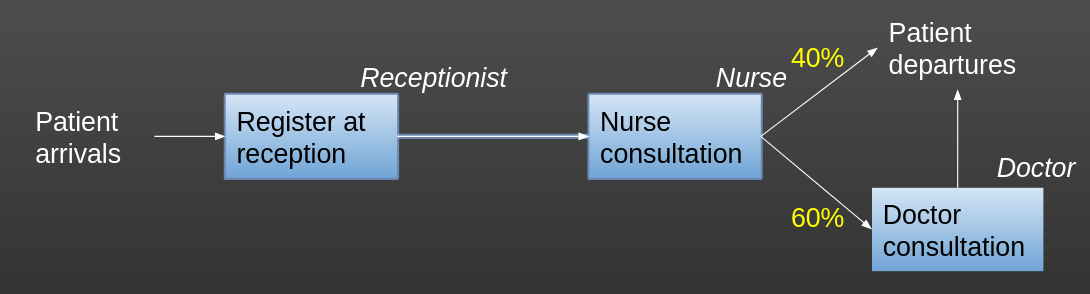
\includegraphics{images/example_simple_model_branching.png}

In the original version of the model, we assumed that there was always a
room available for patients to be seen in. Maybe each nurse and doctor
in this example clinic has their own designated room they are always in.

But let's imagine the setup is slightly different - patients see a
receptionist and go to a waiting area - once both a cubicle and a nurse
are available, the patient is seen by a nurse - if the patient then
needs to see a doctor (which, as before, only a certain \% of patients
will) then they will remain in the same cubicle while waiting for a
doctor - the doctor will see them in the cubicle

The cubicle is released for the next patient after seeing the nurse IF
the patient leaves at this point. Otherwise, it will be released after
seeing the doctor.

\subsection{The g class}\label{the-g-class-9}

We add in an additional parameter for the number of

\begin{Shaded}
\begin{Highlighting}[]
\CommentTok{\# Class to store global parameter values.  We don\textquotesingle{}t create an instance of this}
\CommentTok{\# class {-} we just refer to the class blueprint itself to access the numbers}
\CommentTok{\# inside.}
\KeywordTok{class}\NormalTok{ g:}
\NormalTok{    patient\_inter }\OperatorTok{=} \DecValTok{5}
\NormalTok{    mean\_reception\_time }\OperatorTok{=} \DecValTok{2}
\NormalTok{    mean\_n\_consult\_time }\OperatorTok{=} \DecValTok{6}
\NormalTok{    mean\_d\_consult\_time }\OperatorTok{=} \DecValTok{20}
\NormalTok{    number\_of\_receptionists }\OperatorTok{=} \DecValTok{1}
\NormalTok{    number\_of\_nurses }\OperatorTok{=} \DecValTok{2}
\NormalTok{    number\_of\_doctors }\OperatorTok{=} \DecValTok{2}
\NormalTok{    number\_of\_cubicles }\OperatorTok{=} \DecValTok{5} \CommentTok{\#\#NEW}
\NormalTok{    prob\_seeing\_doctor }\OperatorTok{=} \FloatTok{0.6}
\NormalTok{    sim\_duration }\OperatorTok{=} \DecValTok{1800}
\NormalTok{    number\_of\_runs }\OperatorTok{=} \DecValTok{10}
\end{Highlighting}
\end{Shaded}

\subsection{The Patient class}\label{the-patient-class-8}

We add in an new attribute where we will record the time spent queueing
for a cubicle.

\begin{Shaded}
\begin{Highlighting}[]
\KeywordTok{class}\NormalTok{ Patient:}
    \KeywordTok{def} \FunctionTok{\_\_init\_\_}\NormalTok{(}\VariableTok{self}\NormalTok{, p\_id):}
        \VariableTok{self}\NormalTok{.}\BuiltInTok{id} \OperatorTok{=}\NormalTok{ p\_id}
        \VariableTok{self}\NormalTok{.q\_time\_recep }\OperatorTok{=} \DecValTok{0}
        \VariableTok{self}\NormalTok{.q\_time\_nurse }\OperatorTok{=} \DecValTok{0}
        \VariableTok{self}\NormalTok{.q\_time\_doctor }\OperatorTok{=} \DecValTok{0}
        \VariableTok{self}\NormalTok{.q\_time\_cubicle }\OperatorTok{=} \DecValTok{0} \CommentTok{\#\#NEW}
\end{Highlighting}
\end{Shaded}

\subsection{The model class}\label{the-model-class-9}

\subsubsection{\texorpdfstring{The \textbf{init}
method}{The init method}}\label{the-init-method-10}

We do several things here:

\begin{itemize}
\tightlist
\item
  create a new cubicle resource using the number of cubicles we set in g
\item
  create columns in our patient-level results dataframe for cubicle
  queuing time and time in the cubicle
\item
  add an attribute for storing the average cubicle queueing time
\end{itemize}

\begin{Shaded}
\begin{Highlighting}[]
\KeywordTok{def} \FunctionTok{\_\_init\_\_}\NormalTok{(}\VariableTok{self}\NormalTok{, run\_number):}
        \CommentTok{\# Create a SimPy environment in which everything will live}
        \VariableTok{self}\NormalTok{.env }\OperatorTok{=}\NormalTok{ simpy.Environment()}

        \CommentTok{\# Create a patient counter (which we\textquotesingle{}ll use as a patient ID)}
        \VariableTok{self}\NormalTok{.patient\_counter }\OperatorTok{=} \DecValTok{0}

        \CommentTok{\# Create our resources}
        \VariableTok{self}\NormalTok{.receptionist }\OperatorTok{=}\NormalTok{ simpy.Resource(}\VariableTok{self}\NormalTok{.env, capacity}\OperatorTok{=}\NormalTok{g.number\_of\_receptionists)}
        \VariableTok{self}\NormalTok{.nurse }\OperatorTok{=}\NormalTok{ simpy.Resource(}\VariableTok{self}\NormalTok{.env, capacity}\OperatorTok{=}\NormalTok{g.number\_of\_nurses)}
        \VariableTok{self}\NormalTok{.doctor }\OperatorTok{=}\NormalTok{ simpy.Resource(}\VariableTok{self}\NormalTok{.env, capacity}\OperatorTok{=}\NormalTok{g.number\_of\_doctors)}
        \VariableTok{self}\NormalTok{.cubicle }\OperatorTok{=}\NormalTok{ simpy.Resource(}\VariableTok{self}\NormalTok{.env, capacity}\OperatorTok{=}\NormalTok{g.number\_of\_cubicles) }\CommentTok{\#\# NEW}

        \CommentTok{\# Store the passed in run number}
        \VariableTok{self}\NormalTok{.run\_number }\OperatorTok{=}\NormalTok{ run\_number}

        \CommentTok{\# Create a new Pandas DataFrame that will store some results against}
        \CommentTok{\# the patient ID (which we\textquotesingle{}ll use as the index).}
        \VariableTok{self}\NormalTok{.results\_df }\OperatorTok{=}\NormalTok{ pd.DataFrame()}
        \VariableTok{self}\NormalTok{.results\_df[}\StringTok{"Patient ID"}\NormalTok{] }\OperatorTok{=}\NormalTok{ [}\DecValTok{1}\NormalTok{]}
        \VariableTok{self}\NormalTok{.results\_df[}\StringTok{"Q Time Recep"}\NormalTok{] }\OperatorTok{=}\NormalTok{ [}\FloatTok{0.0}\NormalTok{]}
        \VariableTok{self}\NormalTok{.results\_df[}\StringTok{"Time with Recep"}\NormalTok{] }\OperatorTok{=}\NormalTok{ [}\FloatTok{0.0}\NormalTok{]}
        \VariableTok{self}\NormalTok{.results\_df[}\StringTok{"Q Time Nurse"}\NormalTok{] }\OperatorTok{=}\NormalTok{ [}\FloatTok{0.0}\NormalTok{]}
        \VariableTok{self}\NormalTok{.results\_df[}\StringTok{"Time with Nurse"}\NormalTok{] }\OperatorTok{=}\NormalTok{ [}\FloatTok{0.0}\NormalTok{]}
        \VariableTok{self}\NormalTok{.results\_df[}\StringTok{"Q Time Doctor"}\NormalTok{] }\OperatorTok{=}\NormalTok{ [}\FloatTok{0.0}\NormalTok{]}
        \VariableTok{self}\NormalTok{.results\_df[}\StringTok{"Time with Doctor"}\NormalTok{] }\OperatorTok{=}\NormalTok{ [}\FloatTok{0.0}\NormalTok{]}
        \VariableTok{self}\NormalTok{.results\_df[}\StringTok{"Q Time Cubicle"}\NormalTok{] }\OperatorTok{=}\NormalTok{ [}\FloatTok{0.0}\NormalTok{] }\CommentTok{\#\#NEW}
        \VariableTok{self}\NormalTok{.results\_df[}\StringTok{"Time Using Cubicle"}\NormalTok{] }\OperatorTok{=}\NormalTok{ [}\FloatTok{0.0}\NormalTok{] }\CommentTok{\#\#NEW}
        \VariableTok{self}\NormalTok{.results\_df.set\_index(}\StringTok{"Patient ID"}\NormalTok{, inplace}\OperatorTok{=}\VariableTok{True}\NormalTok{)}

        \CommentTok{\# Create an attribute to store the mean queuing times across this run of}
        \CommentTok{\# the model}
        \VariableTok{self}\NormalTok{.mean\_q\_time\_recep }\OperatorTok{=} \DecValTok{0}
        \VariableTok{self}\NormalTok{.mean\_q\_time\_nurse }\OperatorTok{=} \DecValTok{0}
        \VariableTok{self}\NormalTok{.mean\_q\_time\_doctor }\OperatorTok{=} \DecValTok{0}
        \VariableTok{self}\NormalTok{.mean\_q\_time\_cubicle }\OperatorTok{=} \DecValTok{0} \CommentTok{\#\#NEW}
\end{Highlighting}
\end{Shaded}

\subsection{The generator\_patient\_arrivals
method}\label{the-generator_patient_arrivals-method-3}

This method is unchanged.

\subsection{The attend\_clinic method}\label{the-attend_clinic-method-6}

This is where the majority of our changes take place.

\begin{tcolorbox}[enhanced jigsaw, colframe=quarto-callout-tip-color-frame, bottomtitle=1mm, breakable, rightrule=.15mm, coltitle=black, colbacktitle=quarto-callout-tip-color!10!white, opacityback=0, leftrule=.75mm, arc=.35mm, toptitle=1mm, title=\textcolor{quarto-callout-tip-color}{\faLightbulb}\hspace{0.5em}{Tip}, titlerule=0mm, colback=white, toprule=.15mm, bottomrule=.15mm, left=2mm, opacitybacktitle=0.6]

There are two ways you can request a resource in simpy.

We've used the first method so far:

\begin{Shaded}
\begin{Highlighting}[]
\ControlFlowTok{with} \VariableTok{self}\NormalTok{.receptionist.request() }\ImportTok{as}\NormalTok{ req:}
    \ControlFlowTok{yield}\NormalTok{ req}

    \CommentTok{\#\# the rest of the code you want to run while holding on}
    \CommentTok{\#\# to this resource}
\end{Highlighting}
\end{Shaded}

However, an alternative option is this:

\begin{Shaded}
\begin{Highlighting}[]
\NormalTok{nurse\_request }\OperatorTok{=} \VariableTok{self}\NormalTok{.receptionist.request()}

\ControlFlowTok{yield}\NormalTok{ nurse\_request}

\CommentTok{\#\# the rest of the code you want to run while holding on}
\CommentTok{\#\# to this resource}

\VariableTok{self}\NormalTok{.nurse.release(nurse\_request)}
\end{Highlighting}
\end{Shaded}

Here, we don't use indentation, and instead manually specify when we
stop using the nurse and pass it back to the pool of available
resources.

It's useful to know about this second option as it gives us an easier
way of writing the code for requesting multiple resources at once.

\end{tcolorbox}

Once we finish our time with the receptionist, we are going to record
two attributes.

\begin{Shaded}
\begin{Highlighting}[]
\CommentTok{\# Record the time the patient started queuing for a nurse}
\NormalTok{start\_q\_nurse }\OperatorTok{=} \VariableTok{self}\NormalTok{.env.now}
\NormalTok{start\_q\_cubicle }\OperatorTok{=} \VariableTok{self}\NormalTok{.env.now }\CommentTok{\#\#NEW}
\end{Highlighting}
\end{Shaded}

Yes, they are the same - but it's a bit easier to refer back to them
when they are named separately!

Next we are going to request both a nurse and a cubicle.

\begin{Shaded}
\begin{Highlighting}[]
\NormalTok{nurse\_request }\OperatorTok{=} \VariableTok{self}\NormalTok{.nurse.request()  }\CommentTok{\#\#NEW}
\NormalTok{cubicle\_request }\OperatorTok{=} \VariableTok{self}\NormalTok{.cubicle.request() }\CommentTok{\#\#NEW}
\end{Highlighting}
\end{Shaded}

We then place both of these requests in a list, and wait until either of
them become available.

\begin{Shaded}
\begin{Highlighting}[]
\NormalTok{clinic\_resource }\OperatorTok{=} \ControlFlowTok{yield} \VariableTok{self}\NormalTok{.env.any\_of([nurse\_request,cubicle\_request]) }\CommentTok{\#\#NEW}
\end{Highlighting}
\end{Shaded}

Next, we have to check three possible scenarios and act accordingly: -
both were available at the same time - we got the nurse but are still
waiting for a cubicle - we got the cubicle but are still waiting for a
nurse

\begin{Shaded}
\begin{Highlighting}[]
\NormalTok{clinic\_resource\_list }\OperatorTok{=} \BuiltInTok{list}\NormalTok{(clinic\_resource.keys()) }\CommentTok{\#\#NEW}

\ControlFlowTok{if} \BuiltInTok{len}\NormalTok{(clinic\_resource\_list) }\OperatorTok{\textless{}} \DecValTok{2}\NormalTok{:}
    \CommentTok{\#\# Work out which we didn\textquotesingle{}t get and wait for that one}
\NormalTok{    got\_resource }\OperatorTok{=}\NormalTok{ clinic\_resource\_list[}\DecValTok{0}\NormalTok{]}

    \ControlFlowTok{if}\NormalTok{ got\_resource }\OperatorTok{==}\NormalTok{ nurse\_request:}
\NormalTok{        end\_q\_nurse }\OperatorTok{=} \VariableTok{self}\NormalTok{.env.now}
        \ControlFlowTok{yield}\NormalTok{(cubicle\_request)}
\NormalTok{        end\_q\_cubicle }\OperatorTok{=} \VariableTok{self}\NormalTok{.env.now}
    \ControlFlowTok{else}\NormalTok{:}
\NormalTok{        end\_q\_cubicle }\OperatorTok{=} \VariableTok{self}\NormalTok{.env.now}
        \ControlFlowTok{yield}\NormalTok{(nurse\_request)}
\NormalTok{        end\_q\_nurse }\OperatorTok{=} \VariableTok{self}\NormalTok{.env.now}
\ControlFlowTok{else}\NormalTok{:}
\NormalTok{    end\_q\_cubicle }\OperatorTok{=} \VariableTok{self}\NormalTok{.env.now}
\NormalTok{    end\_q\_nurse }\OperatorTok{=} \VariableTok{self}\NormalTok{.env.now}

\NormalTok{patient.q\_time\_cubicle }\OperatorTok{=}\NormalTok{ end\_q\_cubicle }\OperatorTok{{-}}\NormalTok{ start\_q\_cubicle}

\VariableTok{self}\NormalTok{.results\_df.at[patient.}\BuiltInTok{id}\NormalTok{, }\StringTok{"Q Time Cubicle"}\NormalTok{] }\OperatorTok{=}\NormalTok{ (}
\NormalTok{      patient.q\_time\_cubicle}
\NormalTok{)}

\CommentTok{\# Calculate the time this patient was queuing for the nurse, and}
\CommentTok{\# record it in the patient\textquotesingle{}s attribute for this.}
\NormalTok{patient.q\_time\_nurse }\OperatorTok{=}\NormalTok{ end\_q\_nurse }\OperatorTok{{-}}\NormalTok{ start\_q\_nurse}

\VariableTok{self}\NormalTok{.results\_df.at[patient.}\BuiltInTok{id}\NormalTok{, }\StringTok{"Q Time Nurse"}\NormalTok{] }\OperatorTok{=}\NormalTok{ (}
\NormalTok{  patient.q\_time\_nurse}
\NormalTok{)}
\end{Highlighting}
\end{Shaded}

\begin{tcolorbox}[enhanced jigsaw, colframe=quarto-callout-tip-color-frame, bottomtitle=1mm, breakable, rightrule=.15mm, coltitle=black, colbacktitle=quarto-callout-tip-color!10!white, opacityback=0, leftrule=.75mm, arc=.35mm, toptitle=1mm, title=\textcolor{quarto-callout-tip-color}{\faLightbulb}\hspace{0.5em}{Tip}, titlerule=0mm, colback=white, toprule=.15mm, bottomrule=.15mm, left=2mm, opacitybacktitle=0.6]

Remember - we don't have to indent all of the code where the resource is
used here because we will manually specify when we release it.

You can still use the \emph{first} method of requesting resources on top
of this one - for example, our code for requesting a doctor is
unchanged.

We just don't release the cubicle resource until that section completes.

\end{tcolorbox}

Now, the only thing left to do is to find the right place to release
both resources.

For the nurse, this is after the activity time has elapsed.

\begin{Shaded}
\begin{Highlighting}[]
\CommentTok{\#\# Other code relating to nurse activity...}

\CommentTok{\# Freeze this function in place for the activity time we sampled}
\CommentTok{\# above.  This is the patient spending time with the nurse.}
\ControlFlowTok{yield} \VariableTok{self}\NormalTok{.env.timeout(sampled\_nurse\_act\_time)}

\CommentTok{\# When the time above elapses, the generator function will return}
\CommentTok{\# here.  As there\textquotesingle{}s nothing moref that we\textquotesingle{}ve written, the function}
\CommentTok{\# will simply end.  This is a sink.  We could choose to add}
\CommentTok{\# something here if we wanted to record something {-} e.g. a counter}
\CommentTok{\# for number of patients that left, recording something about the}
\CommentTok{\# patients that left at a particular sink etc.}

\VariableTok{self}\NormalTok{.nurse.release(nurse\_request) }\CommentTok{\#\#NEW}
\end{Highlighting}
\end{Shaded}

Finally, for the cubicle, we don't release this until either after
sampling to decide whether the patient goes on to see a doctor, and
release it accordingly.

Previously we just had an \texttt{if} clause with no \texttt{else} for
seeing the doctor. However, now we need to release the cubicle and
record the total time spent in the cubicle even if they don't see a
doctor, so the \texttt{else} clause becomes necessary.

\begin{Shaded}
\begin{Highlighting}[]
\ControlFlowTok{if}\NormalTok{ random.uniform(}\DecValTok{0}\NormalTok{,}\DecValTok{1}\NormalTok{) }\OperatorTok{\textless{}}\NormalTok{ g.prob\_seeing\_doctor:}
\NormalTok{    start\_q\_doctor }\OperatorTok{=} \VariableTok{self}\NormalTok{.env.now}

    \ControlFlowTok{with} \VariableTok{self}\NormalTok{.doctor.request() }\ImportTok{as}\NormalTok{ req:}
        \ControlFlowTok{yield}\NormalTok{ req}

\NormalTok{        end\_q\_doctor }\OperatorTok{=} \VariableTok{self}\NormalTok{.env.now}

\NormalTok{        patient.q\_time\_doctor }\OperatorTok{=}\NormalTok{ end\_q\_doctor }\OperatorTok{{-}}\NormalTok{ start\_q\_doctor}

\NormalTok{        sampled\_doctor\_act\_time }\OperatorTok{=}\NormalTok{ random.expovariate(}
            \FloatTok{1.0} \OperatorTok{/}\NormalTok{ g.mean\_d\_consult\_time}
\NormalTok{        )}

        \VariableTok{self}\NormalTok{.results\_df.at[patient.}\BuiltInTok{id}\NormalTok{, }\StringTok{"Q Time Doctor"}\NormalTok{] }\OperatorTok{=}\NormalTok{ (}
\NormalTok{            patient.q\_time\_doctor}
\NormalTok{        )}
        \VariableTok{self}\NormalTok{.results\_df.at[patient.}\BuiltInTok{id}\NormalTok{, }\StringTok{"Time with Doctor"}\NormalTok{] }\OperatorTok{=}\NormalTok{ (}
\NormalTok{            sampled\_doctor\_act\_time}
\NormalTok{        )}

        \ControlFlowTok{yield} \VariableTok{self}\NormalTok{.env.timeout(sampled\_doctor\_act\_time)}

        \VariableTok{self}\NormalTok{.results\_df.at[patient.}\BuiltInTok{id}\NormalTok{, }\StringTok{"Time Using Cubicle"}\NormalTok{] }\OperatorTok{=}\NormalTok{ ( }\CommentTok{\#\#NEW}
            \VariableTok{self}\NormalTok{.env.now }\OperatorTok{{-}}\NormalTok{ end\_q\_cubicle}
\NormalTok{        )}

        \VariableTok{self}\NormalTok{.cubicle.release(cubicle\_request) }\CommentTok{\#\#NEW}


\ControlFlowTok{else}\NormalTok{: }\CommentTok{\#\# NEW}

      \VariableTok{self}\NormalTok{.results\_df.at[patient.}\BuiltInTok{id}\NormalTok{, }\StringTok{"Time Using Cubicle"}\NormalTok{] }\OperatorTok{=}\NormalTok{ (  }\CommentTok{\#\#NEW}
            \VariableTok{self}\NormalTok{.env.now }\OperatorTok{{-}}\NormalTok{ end\_q\_cubicle}
\NormalTok{            )}
      \VariableTok{self}\NormalTok{.cubicle.release(cubicle\_request) }\CommentTok{\#\#NEW}
\end{Highlighting}
\end{Shaded}

The only step remaining now is to record the average queueing time for a
cubicle.

\begin{Shaded}
\begin{Highlighting}[]
\VariableTok{self}\NormalTok{.mean\_q\_time\_recep }\OperatorTok{=} \VariableTok{self}\NormalTok{.results\_df[}\StringTok{"Q Time Recep"}\NormalTok{].mean()}
\VariableTok{self}\NormalTok{.mean\_q\_time\_nurse }\OperatorTok{=} \VariableTok{self}\NormalTok{.results\_df[}\StringTok{"Q Time Nurse"}\NormalTok{].mean()}
\VariableTok{self}\NormalTok{.mean\_q\_time\_doctor }\OperatorTok{=} \VariableTok{self}\NormalTok{.results\_df[}\StringTok{"Q Time Doctor"}\NormalTok{].mean()}
\VariableTok{self}\NormalTok{.mean\_q\_time\_cubicle }\OperatorTok{=} \VariableTok{self}\NormalTok{.results\_df[}\StringTok{"Q Time Cubicle"}\NormalTok{].mean() }\CommentTok{\#\#NEW}
\end{Highlighting}
\end{Shaded}

\subsection{The trial class}\label{the-trial-class-9}

\subsubsection{\texorpdfstring{The \textbf{init}
method}{The init method}}\label{the-init-method-11}

In the init method, we add in a column for the average cubicle queue
time per run.

\begin{Shaded}
\begin{Highlighting}[]
\VariableTok{self}\NormalTok{.df\_trial\_results }\OperatorTok{=}\NormalTok{ pd.DataFrame()}
\VariableTok{self}\NormalTok{.df\_trial\_results[}\StringTok{"Run Number"}\NormalTok{] }\OperatorTok{=}\NormalTok{ [}\DecValTok{0}\NormalTok{]}
\VariableTok{self}\NormalTok{.df\_trial\_results[}\StringTok{"Mean Q Time Recep"}\NormalTok{] }\OperatorTok{=}\NormalTok{ [}\FloatTok{0.0}\NormalTok{]}
\VariableTok{self}\NormalTok{.df\_trial\_results[}\StringTok{"Mean Q Time Nurse"}\NormalTok{] }\OperatorTok{=}\NormalTok{ [}\FloatTok{0.0}\NormalTok{]}
\VariableTok{self}\NormalTok{.df\_trial\_results[}\StringTok{"Mean Q Time Doctor"}\NormalTok{] }\OperatorTok{=}\NormalTok{ [}\FloatTok{0.0}\NormalTok{]}
\VariableTok{self}\NormalTok{.df\_trial\_results[}\StringTok{"Mean Q Time Cubicle"}\NormalTok{] }\OperatorTok{=}\NormalTok{ [}\FloatTok{0.0}\NormalTok{] }\CommentTok{\#\#NEW}
\VariableTok{self}\NormalTok{.df\_trial\_results.set\_index(}\StringTok{"Run Number"}\NormalTok{, inplace}\OperatorTok{=}\VariableTok{True}\NormalTok{)}
\end{Highlighting}
\end{Shaded}

\subsubsection{The run method}\label{the-run-method-7}

In the run method, we just need to add the cubcicle queueing mean to the
results dataframe after each run.

After all runs are complete, w can also add in a column that checks
which was longer on average - the queue for the cubicle, or the queue
for the nurse. This can give an indication of which is the limiting
resource.

\begin{Shaded}
\begin{Highlighting}[]
\ControlFlowTok{for}\NormalTok{ run }\KeywordTok{in} \BuiltInTok{range}\NormalTok{(g.number\_of\_runs):}
\NormalTok{    my\_model }\OperatorTok{=}\NormalTok{ Model(run)}
\NormalTok{    my\_model.run()}

    \VariableTok{self}\NormalTok{.df\_trial\_results.loc[run] }\OperatorTok{=}\NormalTok{ [my\_model.mean\_q\_time\_recep,}
\NormalTok{                                      my\_model.mean\_q\_time\_nurse,}
\NormalTok{                                      my\_model.mean\_q\_time\_doctor,}
\NormalTok{                                      my\_model.mean\_q\_time\_cubicle }\CommentTok{\#\#NEW}
\NormalTok{                                      ]}

\CommentTok{\# Once the trial (ie all runs) has completed, add an additional column}
\VariableTok{self}\NormalTok{.df\_trial\_results[}\StringTok{\textquotesingle{}nurse\_queue\_longer\textquotesingle{}}\NormalTok{] }\OperatorTok{=}\NormalTok{ np.where(}\VariableTok{self}\NormalTok{.df\_trial\_results[}\StringTok{\textquotesingle{}Mean Q Time Nurse\textquotesingle{}}\NormalTok{] }\OperatorTok{\textgreater{}} \VariableTok{self}\NormalTok{.df\_trial\_results[}\StringTok{\textquotesingle{}Mean Q Time Cubicle\textquotesingle{}}\NormalTok{], }\VariableTok{True}\NormalTok{, }\VariableTok{False}\NormalTok{) }\CommentTok{\#\#NEW}

\CommentTok{\# Print the final results}
\VariableTok{self}\NormalTok{.print\_trial\_results()}

\BuiltInTok{print}\NormalTok{(}\SpecialStringTok{f"Queue for nurse was longer than queue for cubicle in }\SpecialCharTok{\{}\BuiltInTok{sum}\NormalTok{(}\VariableTok{self}\NormalTok{.df\_trial\_results[}\StringTok{\textquotesingle{}nurse\_queue\_longer\textquotesingle{}}\NormalTok{].values)}\SpecialCharTok{\}}\SpecialStringTok{ trials of }\SpecialCharTok{\{}\NormalTok{g}\SpecialCharTok{.}\NormalTok{number\_of\_runs}\SpecialCharTok{\}}\SpecialStringTok{"}\NormalTok{)}
\end{Highlighting}
\end{Shaded}

\section{The Full Code}\label{the-full-code-9}

\begin{tcolorbox}[enhanced jigsaw, colframe=quarto-callout-note-color-frame, bottomtitle=1mm, breakable, rightrule=.15mm, coltitle=black, colbacktitle=quarto-callout-note-color!10!white, opacityback=0, leftrule=.75mm, arc=.35mm, toptitle=1mm, title=\textcolor{quarto-callout-note-color}{\faInfo}\hspace{0.5em}{Click here to view the full code}, titlerule=0mm, colback=white, toprule=.15mm, bottomrule=.15mm, left=2mm, opacitybacktitle=0.6]

\begin{Shaded}
\begin{Highlighting}[]
\ImportTok{import}\NormalTok{ simpy}
\ImportTok{import}\NormalTok{ random}
\ImportTok{import}\NormalTok{ pandas }\ImportTok{as}\NormalTok{ pd}
\ImportTok{import}\NormalTok{ numpy }\ImportTok{as}\NormalTok{ np }\CommentTok{\#\#NEW}

\CommentTok{\# Class to store global parameter values.  We don\textquotesingle{}t create an instance of this}
\CommentTok{\# class {-} we just refer to the class blueprint itself to access the numbers}
\CommentTok{\# inside.}
\KeywordTok{class}\NormalTok{ g:}
\NormalTok{    patient\_inter }\OperatorTok{=} \DecValTok{5}
\NormalTok{    mean\_reception\_time }\OperatorTok{=} \DecValTok{2}
\NormalTok{    mean\_n\_consult\_time }\OperatorTok{=} \DecValTok{6}
\NormalTok{    mean\_d\_consult\_time }\OperatorTok{=} \DecValTok{20}
\NormalTok{    number\_of\_receptionists }\OperatorTok{=} \DecValTok{1}
\NormalTok{    number\_of\_nurses }\OperatorTok{=} \DecValTok{2}
\NormalTok{    number\_of\_doctors }\OperatorTok{=} \DecValTok{2}
\NormalTok{    number\_of\_cubicles }\OperatorTok{=} \DecValTok{5} \CommentTok{\#\#NEW}
\NormalTok{    prob\_seeing\_doctor }\OperatorTok{=} \FloatTok{0.6}
\NormalTok{    sim\_duration }\OperatorTok{=} \DecValTok{600}
\NormalTok{    number\_of\_runs }\OperatorTok{=} \DecValTok{100}

\CommentTok{\# Class representing patients coming in to the clinic.}
\KeywordTok{class}\NormalTok{ Patient:}
    \KeywordTok{def} \FunctionTok{\_\_init\_\_}\NormalTok{(}\VariableTok{self}\NormalTok{, p\_id):}
        \VariableTok{self}\NormalTok{.}\BuiltInTok{id} \OperatorTok{=}\NormalTok{ p\_id}
        \VariableTok{self}\NormalTok{.q\_time\_recep }\OperatorTok{=} \DecValTok{0}
        \VariableTok{self}\NormalTok{.q\_time\_nurse }\OperatorTok{=} \DecValTok{0}
        \VariableTok{self}\NormalTok{.q\_time\_doctor }\OperatorTok{=} \DecValTok{0}
        \VariableTok{self}\NormalTok{.q\_time\_cubicle }\OperatorTok{=} \DecValTok{0} \CommentTok{\#\#NEW}

\CommentTok{\# Class representing our model of the clinic.}
\KeywordTok{class}\NormalTok{ Model:}
    \CommentTok{\# Constructor to set up the model for a run.  We pass in a run number when}
    \CommentTok{\# we create a new model.}
    \KeywordTok{def} \FunctionTok{\_\_init\_\_}\NormalTok{(}\VariableTok{self}\NormalTok{, run\_number):}
        \CommentTok{\# Create a SimPy environment in which everything will live}
        \VariableTok{self}\NormalTok{.env }\OperatorTok{=}\NormalTok{ simpy.Environment()}

        \CommentTok{\# Create a patient counter (which we\textquotesingle{}ll use as a patient ID)}
        \VariableTok{self}\NormalTok{.patient\_counter }\OperatorTok{=} \DecValTok{0}

        \CommentTok{\# Create our resources}
        \VariableTok{self}\NormalTok{.receptionist }\OperatorTok{=}\NormalTok{ simpy.Resource(}\VariableTok{self}\NormalTok{.env, capacity}\OperatorTok{=}\NormalTok{g.number\_of\_receptionists)}
        \VariableTok{self}\NormalTok{.nurse }\OperatorTok{=}\NormalTok{ simpy.Resource(}\VariableTok{self}\NormalTok{.env, capacity}\OperatorTok{=}\NormalTok{g.number\_of\_nurses)}
        \VariableTok{self}\NormalTok{.doctor }\OperatorTok{=}\NormalTok{ simpy.Resource(}\VariableTok{self}\NormalTok{.env, capacity}\OperatorTok{=}\NormalTok{g.number\_of\_doctors)}
        \VariableTok{self}\NormalTok{.cubicle }\OperatorTok{=}\NormalTok{ simpy.Resource(}\VariableTok{self}\NormalTok{.env, capacity}\OperatorTok{=}\NormalTok{g.number\_of\_cubicles) }\CommentTok{\#\# NEW}

        \CommentTok{\# Store the passed in run number}
        \VariableTok{self}\NormalTok{.run\_number }\OperatorTok{=}\NormalTok{ run\_number}

        \CommentTok{\# Create a new Pandas DataFrame that will store some results against}
        \CommentTok{\# the patient ID (which we\textquotesingle{}ll use as the index).}
        \VariableTok{self}\NormalTok{.results\_df }\OperatorTok{=}\NormalTok{ pd.DataFrame()}
        \VariableTok{self}\NormalTok{.results\_df[}\StringTok{"Patient ID"}\NormalTok{] }\OperatorTok{=}\NormalTok{ [}\DecValTok{1}\NormalTok{]}
        \VariableTok{self}\NormalTok{.results\_df[}\StringTok{"Q Time Recep"}\NormalTok{] }\OperatorTok{=}\NormalTok{ [}\FloatTok{0.0}\NormalTok{]}
        \VariableTok{self}\NormalTok{.results\_df[}\StringTok{"Time with Recep"}\NormalTok{] }\OperatorTok{=}\NormalTok{ [}\FloatTok{0.0}\NormalTok{]}
        \VariableTok{self}\NormalTok{.results\_df[}\StringTok{"Q Time Nurse"}\NormalTok{] }\OperatorTok{=}\NormalTok{ [}\FloatTok{0.0}\NormalTok{]}
        \VariableTok{self}\NormalTok{.results\_df[}\StringTok{"Time with Nurse"}\NormalTok{] }\OperatorTok{=}\NormalTok{ [}\FloatTok{0.0}\NormalTok{]}
        \VariableTok{self}\NormalTok{.results\_df[}\StringTok{"Q Time Doctor"}\NormalTok{] }\OperatorTok{=}\NormalTok{ [}\FloatTok{0.0}\NormalTok{]}
        \VariableTok{self}\NormalTok{.results\_df[}\StringTok{"Time with Doctor"}\NormalTok{] }\OperatorTok{=}\NormalTok{ [}\FloatTok{0.0}\NormalTok{]}
        \VariableTok{self}\NormalTok{.results\_df[}\StringTok{"Q Time Cubicle"}\NormalTok{] }\OperatorTok{=}\NormalTok{ [}\FloatTok{0.0}\NormalTok{] }\CommentTok{\#\#NEW}
        \VariableTok{self}\NormalTok{.results\_df[}\StringTok{"Time Using Cubicle"}\NormalTok{] }\OperatorTok{=}\NormalTok{ [}\FloatTok{0.0}\NormalTok{] }\CommentTok{\#\#NEW}
        \VariableTok{self}\NormalTok{.results\_df.set\_index(}\StringTok{"Patient ID"}\NormalTok{, inplace}\OperatorTok{=}\VariableTok{True}\NormalTok{)}

        \CommentTok{\# Create an attribute to store the mean queuing times across this run of}
        \CommentTok{\# the model}
        \VariableTok{self}\NormalTok{.mean\_q\_time\_recep }\OperatorTok{=} \DecValTok{0}
        \VariableTok{self}\NormalTok{.mean\_q\_time\_nurse }\OperatorTok{=} \DecValTok{0}
        \VariableTok{self}\NormalTok{.mean\_q\_time\_doctor }\OperatorTok{=} \DecValTok{0}
        \VariableTok{self}\NormalTok{.mean\_q\_time\_cubicle }\OperatorTok{=} \DecValTok{0} \CommentTok{\#\#NEW}

    \CommentTok{\# A generator function that represents the DES generator for patient}
    \CommentTok{\# arrivals}
    \KeywordTok{def}\NormalTok{ generator\_patient\_arrivals(}\VariableTok{self}\NormalTok{):}
        \CommentTok{\# We use an infinite loop here to keep doing this indefinitely whilst}
        \CommentTok{\# the simulation runs}
        \ControlFlowTok{while} \VariableTok{True}\NormalTok{:}
            \CommentTok{\# Increment the patient counter by 1 (this means our first patient}
            \CommentTok{\# will have an ID of 1)}
            \VariableTok{self}\NormalTok{.patient\_counter }\OperatorTok{+=} \DecValTok{1}

            \CommentTok{\# Create a new patient {-} an instance of the Patient Class we}
            \CommentTok{\# defined above.  Remember, we pass in the ID when creating a}
            \CommentTok{\# patient {-} so here we pass the patient counter to use as the ID.}
\NormalTok{            p }\OperatorTok{=}\NormalTok{ Patient(}\VariableTok{self}\NormalTok{.patient\_counter)}

            \CommentTok{\# Tell SimPy to start up the attend\_clinic generator function with}
            \CommentTok{\# this patient (the generator function that will model the}
            \CommentTok{\# patient\textquotesingle{}s journey through the system)}
            \VariableTok{self}\NormalTok{.env.process(}\VariableTok{self}\NormalTok{.attend\_clinic(p))}

            \CommentTok{\# Randomly sample the time to the next patient arriving.  Here, we}
            \CommentTok{\# sample from an exponential distribution (common for inter{-}arrival}
            \CommentTok{\# times), and pass in a lambda value of 1 / mean.  The mean}
            \CommentTok{\# inter{-}arrival time is stored in the g class.}
\NormalTok{            sampled\_inter }\OperatorTok{=}\NormalTok{ random.expovariate(}\FloatTok{1.0} \OperatorTok{/}\NormalTok{ g.patient\_inter)}

            \CommentTok{\# Freeze this instance of this function in place until the}
            \CommentTok{\# inter{-}arrival time we sampled above has elapsed.  Note {-} time in}
            \CommentTok{\# SimPy progresses in "Time Units", which can represent anything}
            \CommentTok{\# you like (just make sure you\textquotesingle{}re consistent within the model)}
            \ControlFlowTok{yield} \VariableTok{self}\NormalTok{.env.timeout(sampled\_inter)}

    \CommentTok{\# A generator function that represents the pathway for a patient going}
    \CommentTok{\# through the clinic.}
    \CommentTok{\# The patient object is passed in to the generator function so we can}
    \CommentTok{\# extract information from / record information to it}
    \KeywordTok{def}\NormalTok{ attend\_clinic(}\VariableTok{self}\NormalTok{, patient):}
\NormalTok{        start\_q\_recep }\OperatorTok{=} \VariableTok{self}\NormalTok{.env.now}

        \ControlFlowTok{with} \VariableTok{self}\NormalTok{.receptionist.request() }\ImportTok{as}\NormalTok{ req:}
            \ControlFlowTok{yield}\NormalTok{ req}

\NormalTok{            end\_q\_recep }\OperatorTok{=} \VariableTok{self}\NormalTok{.env.now}

\NormalTok{            patient.q\_time\_recep }\OperatorTok{=}\NormalTok{ end\_q\_recep }\OperatorTok{{-}}\NormalTok{ start\_q\_recep}

\NormalTok{            sampled\_recep\_act\_time }\OperatorTok{=}\NormalTok{ random.expovariate(}
                \FloatTok{1.0} \OperatorTok{/}\NormalTok{ g.mean\_reception\_time}
\NormalTok{            )}

            \VariableTok{self}\NormalTok{.results\_df.at[patient.}\BuiltInTok{id}\NormalTok{, }\StringTok{"Q Time Recep"}\NormalTok{] }\OperatorTok{=}\NormalTok{ (}
\NormalTok{                 patient.q\_time\_recep}
\NormalTok{            )}
            \VariableTok{self}\NormalTok{.results\_df.at[patient.}\BuiltInTok{id}\NormalTok{, }\StringTok{"Time with Recep"}\NormalTok{] }\OperatorTok{=}\NormalTok{ (}
\NormalTok{                 sampled\_recep\_act\_time}
\NormalTok{            )}

            \ControlFlowTok{yield} \VariableTok{self}\NormalTok{.env.timeout(sampled\_recep\_act\_time)}

        \CommentTok{\# Here\textquotesingle{}s where the patient finishes with the receptionist, and starts}
        \CommentTok{\# queuing for the nurse}
        \CommentTok{\# NEW: They will also be queueing for a cubicle at this point.}
        \CommentTok{\#}

        \CommentTok{\# Record the time the patient started queuing for a nurse}
\NormalTok{        start\_q\_nurse }\OperatorTok{=} \VariableTok{self}\NormalTok{.env.now}
\NormalTok{        start\_q\_cubicle }\OperatorTok{=} \VariableTok{self}\NormalTok{.env.now }\CommentTok{\#\#NEW}

        \CommentTok{\#\#\#\#\#\#\#\#}
        \CommentTok{\#\#NEW}
        \CommentTok{\#\#\#\#\#\#\#\#}
        \CommentTok{\# As we are going to require the cubicle for the entire time period from}
        \CommentTok{\# here on, and won\textquotesingle{}t release it until they exit the system, we will request}
        \CommentTok{\# the cubicle here and indent all of the existing code by one level.}

\NormalTok{        nurse\_request }\OperatorTok{=} \VariableTok{self}\NormalTok{.nurse.request()  }\CommentTok{\#\#NEW}
\NormalTok{        cubicle\_request }\OperatorTok{=} \VariableTok{self}\NormalTok{.cubicle.request() }\CommentTok{\#\#NEW}

\NormalTok{        clinic\_resource }\OperatorTok{=} \ControlFlowTok{yield} \VariableTok{self}\NormalTok{.env.any\_of([nurse\_request,cubicle\_request]) }\CommentTok{\#\#NEW}

        \CommentTok{\# First, check if both were available at once. If so, we can continue.}

\NormalTok{        clinic\_resource\_list }\OperatorTok{=} \BuiltInTok{list}\NormalTok{(clinic\_resource.keys()) }\CommentTok{\#\#NEW}

        \ControlFlowTok{if} \BuiltInTok{len}\NormalTok{(clinic\_resource\_list) }\OperatorTok{\textless{}} \DecValTok{2}\NormalTok{:}
            \CommentTok{\#\# Work out which we didn\textquotesingle{}t get and wait for that one}
\NormalTok{            got\_resource }\OperatorTok{=}\NormalTok{ clinic\_resource\_list[}\DecValTok{0}\NormalTok{]}

            \ControlFlowTok{if}\NormalTok{ got\_resource }\OperatorTok{==}\NormalTok{ nurse\_request:}
                \CommentTok{\#print(f"\{patient.id\} got nurse first at \{self.env.now\}")}
\NormalTok{                end\_q\_nurse }\OperatorTok{=} \VariableTok{self}\NormalTok{.env.now}
                \ControlFlowTok{yield}\NormalTok{(cubicle\_request)}
\NormalTok{                end\_q\_cubicle }\OperatorTok{=} \VariableTok{self}\NormalTok{.env.now}
                \CommentTok{\#print(f"\{patient.id\} got cubicle at \{self.env.now\}")}
            \ControlFlowTok{else}\NormalTok{:}
                \CommentTok{\#print(f"\{patient.id\} got cubicle first at \{self.env.now\}")}
\NormalTok{                end\_q\_cubicle }\OperatorTok{=} \VariableTok{self}\NormalTok{.env.now}
                \ControlFlowTok{yield}\NormalTok{(nurse\_request)}
\NormalTok{                end\_q\_nurse }\OperatorTok{=} \VariableTok{self}\NormalTok{.env.now}
                \CommentTok{\#print(f"\{patient.id\} got nurse at \{self.env.now\}")}
        \ControlFlowTok{else}\NormalTok{:}
            \CommentTok{\#print(f"\{patient.id\} got both resources simultaneously at \{self.env.now\}")}
\NormalTok{            end\_q\_cubicle }\OperatorTok{=} \VariableTok{self}\NormalTok{.env.now}
\NormalTok{            end\_q\_nurse }\OperatorTok{=} \VariableTok{self}\NormalTok{.env.now}

\NormalTok{        patient.q\_time\_cubicle }\OperatorTok{=}\NormalTok{ end\_q\_cubicle }\OperatorTok{{-}}\NormalTok{ start\_q\_cubicle}

        \VariableTok{self}\NormalTok{.results\_df.at[patient.}\BuiltInTok{id}\NormalTok{, }\StringTok{"Q Time Cubicle"}\NormalTok{] }\OperatorTok{=}\NormalTok{ (}
\NormalTok{              patient.q\_time\_cubicle}
\NormalTok{        )}

        \CommentTok{\# Calculate the time this patient was queuing for the nurse, and}
        \CommentTok{\# record it in the patient\textquotesingle{}s attribute for this.}
\NormalTok{        patient.q\_time\_nurse }\OperatorTok{=}\NormalTok{ end\_q\_nurse }\OperatorTok{{-}}\NormalTok{ start\_q\_nurse}

        \VariableTok{self}\NormalTok{.results\_df.at[patient.}\BuiltInTok{id}\NormalTok{, }\StringTok{"Q Time Nurse"}\NormalTok{] }\OperatorTok{=}\NormalTok{ (}
\NormalTok{          patient.q\_time\_nurse}
\NormalTok{        )}
        \CommentTok{\#\#\#\#\#\#\#\#}
        \CommentTok{\#\#}\RegionMarkerTok{END}\CommentTok{ NEW}
        \CommentTok{\#\#\#\#\#\#\#\#}

        \CommentTok{\# Now we\textquotesingle{}ll randomly sample the time this patient with the nurse.}
        \CommentTok{\# Here, we use an Exponential distribution for simplicity, but you}
        \CommentTok{\# would typically use a Log Normal distribution for a real model}
        \CommentTok{\# (we\textquotesingle{}ll come back to that).  As with sampling the inter{-}arrival}
        \CommentTok{\# times, we grab the mean from the g class, and pass in 1 / mean}
        \CommentTok{\# as the lambda value.}
\NormalTok{        sampled\_nurse\_act\_time }\OperatorTok{=}\NormalTok{ random.expovariate(}\FloatTok{1.0} \OperatorTok{/}
\NormalTok{                                                    g.mean\_n\_consult\_time)}

        \CommentTok{\# Here we\textquotesingle{}ll store the queuing time for the nurse and the sampled}
        \CommentTok{\# time to spend with the nurse in the results DataFrame against the}
        \CommentTok{\# ID for this patient.  In real world models, you may not want to}
        \CommentTok{\# bother storing the sampled activity times {-} but as this is a}
        \CommentTok{\# simple model, we\textquotesingle{}ll do it here.}
        \CommentTok{\# We use a handy property of pandas called .at, which works a bit}
        \CommentTok{\# like .loc.  .at allows us to access (and therefore change) a}
        \CommentTok{\# particular cell in our DataFrame by providing the row and column.}
        \CommentTok{\# Here, we specify the row as the patient ID (the index), and the}
        \CommentTok{\# column for the value we want to update for that patient.}
        \VariableTok{self}\NormalTok{.results\_df.at[patient.}\BuiltInTok{id}\NormalTok{, }\StringTok{"Time with Nurse"}\NormalTok{] }\OperatorTok{=}\NormalTok{ (}
\NormalTok{            sampled\_nurse\_act\_time)}

        \CommentTok{\# Freeze this function in place for the activity time we sampled}
        \CommentTok{\# above.  This is the patient spending time with the nurse.}
        \ControlFlowTok{yield} \VariableTok{self}\NormalTok{.env.timeout(sampled\_nurse\_act\_time)}

        \CommentTok{\# When the time above elapses, the generator function will return}
        \CommentTok{\# here.  As there\textquotesingle{}s nothing moref that we\textquotesingle{}ve written, the function}
        \CommentTok{\# will simply end.  This is a sink.  We could choose to add}
        \CommentTok{\# something here if we wanted to record something {-} e.g. a counter}
        \CommentTok{\# for number of patients that left, recording something about the}
        \CommentTok{\# patients that left at a particular sink etc.}

        \VariableTok{self}\NormalTok{.nurse.release(nurse\_request) }\CommentTok{\#\#NEW}

        \CommentTok{\# Conditional logic to see if patient goes on to see doctor}
        \CommentTok{\# We sample from the uniform distribution between 0 and 1.  If the value}
        \CommentTok{\# is less than the probability of seeing a doctor (stored in g Class)}
        \CommentTok{\# then we say the patient sees a doctor.}
        \CommentTok{\# If not, this block of code won\textquotesingle{}t be run and the patient will just}
        \CommentTok{\# leave the system (we could add in an else if we wanted a branching}
        \CommentTok{\# path to another activity instead)}
        \ControlFlowTok{if}\NormalTok{ random.uniform(}\DecValTok{0}\NormalTok{,}\DecValTok{1}\NormalTok{) }\OperatorTok{\textless{}}\NormalTok{ g.prob\_seeing\_doctor:}
\NormalTok{            start\_q\_doctor }\OperatorTok{=} \VariableTok{self}\NormalTok{.env.now}

            \ControlFlowTok{with} \VariableTok{self}\NormalTok{.doctor.request() }\ImportTok{as}\NormalTok{ req:}
                \ControlFlowTok{yield}\NormalTok{ req}

\NormalTok{                end\_q\_doctor }\OperatorTok{=} \VariableTok{self}\NormalTok{.env.now}

\NormalTok{                patient.q\_time\_doctor }\OperatorTok{=}\NormalTok{ end\_q\_doctor }\OperatorTok{{-}}\NormalTok{ start\_q\_doctor}

\NormalTok{                sampled\_doctor\_act\_time }\OperatorTok{=}\NormalTok{ random.expovariate(}
                    \FloatTok{1.0} \OperatorTok{/}\NormalTok{ g.mean\_d\_consult\_time}
\NormalTok{                )}

                \VariableTok{self}\NormalTok{.results\_df.at[patient.}\BuiltInTok{id}\NormalTok{, }\StringTok{"Q Time Doctor"}\NormalTok{] }\OperatorTok{=}\NormalTok{ (}
\NormalTok{                    patient.q\_time\_doctor}
\NormalTok{                )}
                \VariableTok{self}\NormalTok{.results\_df.at[patient.}\BuiltInTok{id}\NormalTok{, }\StringTok{"Time with Doctor"}\NormalTok{] }\OperatorTok{=}\NormalTok{ (}
\NormalTok{                    sampled\_doctor\_act\_time}
\NormalTok{                )}

                \ControlFlowTok{yield} \VariableTok{self}\NormalTok{.env.timeout(sampled\_doctor\_act\_time)}

                \VariableTok{self}\NormalTok{.results\_df.at[patient.}\BuiltInTok{id}\NormalTok{, }\StringTok{"Time Using Cubicle"}\NormalTok{] }\OperatorTok{=}\NormalTok{ ( }\CommentTok{\#\#NEW}
                    \VariableTok{self}\NormalTok{.env.now }\OperatorTok{{-}}\NormalTok{ end\_q\_cubicle}
\NormalTok{                )}

                \VariableTok{self}\NormalTok{.cubicle.release(cubicle\_request) }\CommentTok{\#\#NEW}

        \ControlFlowTok{else}\NormalTok{: }\CommentTok{\#\# NEW}

            \VariableTok{self}\NormalTok{.results\_df.at[patient.}\BuiltInTok{id}\NormalTok{, }\StringTok{"Time Using Cubicle"}\NormalTok{] }\OperatorTok{=}\NormalTok{ (  }\CommentTok{\#\#NEW}
                  \VariableTok{self}\NormalTok{.env.now }\OperatorTok{{-}}\NormalTok{ end\_q\_cubicle}
\NormalTok{                  )}
            \VariableTok{self}\NormalTok{.cubicle.release(cubicle\_request) }\CommentTok{\#\#NEW}


    \CommentTok{\# This method calculates results over a single run.  Here we just calculate}
    \CommentTok{\# a mean, but in real world models you\textquotesingle{}d probably want to calculate more.}
    \KeywordTok{def}\NormalTok{ calculate\_run\_results(}\VariableTok{self}\NormalTok{):}
        \CommentTok{\# Take the mean of the queuing times across patients in this run of the}
        \CommentTok{\# model.}
        \VariableTok{self}\NormalTok{.mean\_q\_time\_recep }\OperatorTok{=} \VariableTok{self}\NormalTok{.results\_df[}\StringTok{"Q Time Recep"}\NormalTok{].mean()}
        \VariableTok{self}\NormalTok{.mean\_q\_time\_nurse }\OperatorTok{=} \VariableTok{self}\NormalTok{.results\_df[}\StringTok{"Q Time Nurse"}\NormalTok{].mean()}
        \VariableTok{self}\NormalTok{.mean\_q\_time\_doctor }\OperatorTok{=} \VariableTok{self}\NormalTok{.results\_df[}\StringTok{"Q Time Doctor"}\NormalTok{].mean()}
        \VariableTok{self}\NormalTok{.mean\_q\_time\_cubicle }\OperatorTok{=} \VariableTok{self}\NormalTok{.results\_df[}\StringTok{"Q Time Cubicle"}\NormalTok{].mean() }\CommentTok{\#\#NEW}

    \CommentTok{\# The run method starts up the DES entity generators, runs the simulation,}
    \CommentTok{\# and in turns calls anything we need to generate results for the run}
    \KeywordTok{def}\NormalTok{ run(}\VariableTok{self}\NormalTok{):}
        \CommentTok{\# Start up our DES entity generators that create new patients.  We\textquotesingle{}ve}
        \CommentTok{\# only got one in this model, but we\textquotesingle{}d need to do this for each one if}
        \CommentTok{\# we had multiple generators.}
        \VariableTok{self}\NormalTok{.env.process(}\VariableTok{self}\NormalTok{.generator\_patient\_arrivals())}

        \CommentTok{\# Run the model for the duration specified in g class}
        \VariableTok{self}\NormalTok{.env.run(until}\OperatorTok{=}\NormalTok{g.sim\_duration)}

        \CommentTok{\# Now the simulation run has finished, call the method that calculates}
        \CommentTok{\# run results}
        \VariableTok{self}\NormalTok{.calculate\_run\_results()}

        \CommentTok{\# Print the run number with the patient{-}level results from this run of}
        \CommentTok{\# the model}
        \CommentTok{\# EDIT: Omit patient{-}level results in this model}
        \CommentTok{\# print (f"Run Number \{self.run\_number\}")}
        \CommentTok{\# print (self.results\_df)}

\CommentTok{\# Class representing a Trial for our simulation {-} a batch of simulation runs.}
\KeywordTok{class}\NormalTok{ Trial:}
    \CommentTok{\# The constructor sets up a pandas dataframe that will store the key}
    \CommentTok{\# results from each run against run number, with run number as the index.}
    \KeywordTok{def}  \FunctionTok{\_\_init\_\_}\NormalTok{(}\VariableTok{self}\NormalTok{):}
        \VariableTok{self}\NormalTok{.df\_trial\_results }\OperatorTok{=}\NormalTok{ pd.DataFrame()}
        \VariableTok{self}\NormalTok{.df\_trial\_results[}\StringTok{"Run Number"}\NormalTok{] }\OperatorTok{=}\NormalTok{ [}\DecValTok{0}\NormalTok{]}
        \VariableTok{self}\NormalTok{.df\_trial\_results[}\StringTok{"Mean Q Time Recep"}\NormalTok{] }\OperatorTok{=}\NormalTok{ [}\FloatTok{0.0}\NormalTok{]}
        \VariableTok{self}\NormalTok{.df\_trial\_results[}\StringTok{"Mean Q Time Nurse"}\NormalTok{] }\OperatorTok{=}\NormalTok{ [}\FloatTok{0.0}\NormalTok{]}
        \VariableTok{self}\NormalTok{.df\_trial\_results[}\StringTok{"Mean Q Time Doctor"}\NormalTok{] }\OperatorTok{=}\NormalTok{ [}\FloatTok{0.0}\NormalTok{]}
        \VariableTok{self}\NormalTok{.df\_trial\_results[}\StringTok{"Mean Q Time Cubicle"}\NormalTok{] }\OperatorTok{=}\NormalTok{ [}\FloatTok{0.0}\NormalTok{] }\CommentTok{\#\#NEW}
        \VariableTok{self}\NormalTok{.df\_trial\_results.set\_index(}\StringTok{"Run Number"}\NormalTok{, inplace}\OperatorTok{=}\VariableTok{True}\NormalTok{)}

    \CommentTok{\# Method to print out the results from the trial.  In real world models,}
    \CommentTok{\# you\textquotesingle{}d likely save them as well as (or instead of) printing them}
    \KeywordTok{def}\NormalTok{ print\_trial\_results(}\VariableTok{self}\NormalTok{):}
        \BuiltInTok{print}\NormalTok{ (}\StringTok{"Trial Results"}\NormalTok{)}
        \BuiltInTok{print}\NormalTok{ (}\VariableTok{self}\NormalTok{.df\_trial\_results.}\BuiltInTok{round}\NormalTok{(}\DecValTok{1}\NormalTok{)) }\CommentTok{\#\#EDITED: Added rounding}

    \CommentTok{\# Method to run a trial}
    \KeywordTok{def}\NormalTok{ run\_trial(}\VariableTok{self}\NormalTok{):}
        \CommentTok{\# Run the simulation for the number of runs specified in g class.}
        \CommentTok{\# For each run, we create a new instance of the Model class and call its}
        \CommentTok{\# run method, which sets everything else in motion.  Once the run has}
        \CommentTok{\# completed, we grab out the stored run results (just mean queuing time}
        \CommentTok{\# here) and store it against the run number in the trial results}
        \CommentTok{\# dataframe.}
        \ControlFlowTok{for}\NormalTok{ run }\KeywordTok{in} \BuiltInTok{range}\NormalTok{(g.number\_of\_runs):}
\NormalTok{            my\_model }\OperatorTok{=}\NormalTok{ Model(run)}
\NormalTok{            my\_model.run()}

            \VariableTok{self}\NormalTok{.df\_trial\_results.loc[run] }\OperatorTok{=}\NormalTok{ [my\_model.mean\_q\_time\_recep,}
\NormalTok{                                              my\_model.mean\_q\_time\_nurse,}
\NormalTok{                                              my\_model.mean\_q\_time\_doctor,}
\NormalTok{                                              my\_model.mean\_q\_time\_cubicle }\CommentTok{\#\#NEW}
\NormalTok{                                              ]}

        \CommentTok{\# Once the trial (ie all runs) has completed, add an additional column}
        \VariableTok{self}\NormalTok{.df\_trial\_results[}\StringTok{\textquotesingle{}nurse\_queue\_longer\textquotesingle{}}\NormalTok{] }\OperatorTok{=}\NormalTok{ np.where(}\VariableTok{self}\NormalTok{.df\_trial\_results[}\StringTok{\textquotesingle{}Mean Q Time Nurse\textquotesingle{}}\NormalTok{] }\OperatorTok{\textgreater{}} \VariableTok{self}\NormalTok{.df\_trial\_results[}\StringTok{\textquotesingle{}Mean Q Time Cubicle\textquotesingle{}}\NormalTok{], }\VariableTok{True}\NormalTok{, }\VariableTok{False}\NormalTok{) }\CommentTok{\#\#NEW}

        \CommentTok{\# Print the final results}
        \VariableTok{self}\NormalTok{.print\_trial\_results()}

        \BuiltInTok{print}\NormalTok{(}\SpecialStringTok{f"Queue for nurse was longer than queue for cubicle in }\SpecialCharTok{\{}\BuiltInTok{sum}\NormalTok{(}\VariableTok{self}\NormalTok{.df\_trial\_results[}\StringTok{\textquotesingle{}nurse\_queue\_longer\textquotesingle{}}\NormalTok{].values)}\SpecialCharTok{\}}\SpecialStringTok{ trials of }\SpecialCharTok{\{}\NormalTok{g}\SpecialCharTok{.}\NormalTok{number\_of\_runs}\SpecialCharTok{\}}\SpecialStringTok{"}\NormalTok{)}
\end{Highlighting}
\end{Shaded}

\end{tcolorbox}

\section{Evaluating the outputs}\label{evaluating-the-outputs-8}

\begin{tcolorbox}[enhanced jigsaw, colframe=quarto-callout-warning-color-frame, bottomtitle=1mm, breakable, rightrule=.15mm, coltitle=black, colbacktitle=quarto-callout-warning-color!10!white, opacityback=0, leftrule=.75mm, arc=.35mm, toptitle=1mm, title=\textcolor{quarto-callout-warning-color}{\faExclamationTriangle}\hspace{0.5em}{Warning}, titlerule=0mm, colback=white, toprule=.15mm, bottomrule=.15mm, left=2mm, opacitybacktitle=0.6]

We haven't fully controlled the randomness in our trials here, so the
different trials will each have slightly differing arrival times and
activity times. Even though we have run a high number of trials to
compensate, this is not an ideal solution.

For information on how to properly control for randomness across trials,
make sure to read the reproducibility section
(Chapter~\ref{sec-reproducibility}).

\end{tcolorbox}

\begin{verbatim}
9 cubicles, 2 nurses, 2 doctors
Trial Results
            Mean Q Time Recep  Mean Q Time Nurse  Mean Q Time Doctor  \
Run Number                                                             
0                         0.6                3.3                30.4   
1                         0.8               51.3                36.0   
2                         1.6                3.9                24.5   
3                         2.0               27.8                34.2   
4                         1.0                4.2                16.0   
...                       ...                ...                 ...   
95                        1.2               28.5                37.4   
96                        1.3               52.0                48.8   
97                        0.8               24.3                41.8   
98                        1.1               32.2                42.6   
99                        1.4               29.1                46.9   

            Mean Q Time Cubicle  nurse_queue_longer  
Run Number                                           
0                           4.4               False  
1                          51.2                True  
2                           2.4                True  
3                          28.6               False  
4                           0.5                True  
...                         ...                 ...  
95                         30.5               False  
96                         54.9               False  
97                         27.0               False  
98                         34.3               False  
99                         33.0               False  

[100 rows x 5 columns]
Queue for nurse was longer than queue for cubicle in 27 trials of 100
\end{verbatim}

\begin{verbatim}
3 cubicles, 2 nurses, 2 doctors
Trial Results
            Mean Q Time Recep  Mean Q Time Nurse  Mean Q Time Doctor  \
Run Number                                                             
0                         1.0              100.0                 4.1   
1                         0.8              118.5                 4.8   
2                         1.6              107.1                 4.7   
3                         1.4               66.2                 4.3   
4                         0.8               46.5                 2.5   
...                       ...                ...                 ...   
95                        0.7               74.5                 3.4   
96                        1.5               55.4                 3.3   
97                        0.7               66.6                 4.3   
98                        1.1               53.6                 3.5   
99                        0.7               28.5                 3.5   

            Mean Q Time Cubicle  nurse_queue_longer  
Run Number                                           
0                         107.2               False  
1                         127.3               False  
2                         115.2               False  
3                          73.3               False  
4                          51.9               False  
...                         ...                 ...  
95                         80.9               False  
96                         61.3               False  
97                         73.7               False  
98                         60.0               False  
99                         34.5               False  

[100 rows x 5 columns]
Queue for nurse was longer than queue for cubicle in 0 trials of 100
\end{verbatim}

\begin{verbatim}
12 cubicles, 2 nurses, 2 doctors
Trial Results
            Mean Q Time Recep  Mean Q Time Nurse  Mean Q Time Doctor  \
Run Number                                                             
0                         1.1                1.6                36.6   
1                         0.6                3.5                47.7   
2                         1.1                2.5                11.2   
3                         1.5                8.3                32.9   
4                         2.2               29.8                81.2   
...                       ...                ...                 ...   
95                        2.1               50.9                63.8   
96                        0.9               11.3                53.8   
97                        0.8                1.2                16.3   
98                        1.5                0.9                25.3   
99                        1.2               22.4                78.2   

            Mean Q Time Cubicle  nurse_queue_longer  
Run Number                                           
0                           0.4                True  
1                           2.1                True  
2                           0.0                True  
3                           7.8                True  
4                          33.7               False  
...                         ...                 ...  
95                         51.0               False  
96                         11.3                True  
97                          0.0                True  
98                          0.4                True  
99                         26.7               False  

[100 rows x 5 columns]
Queue for nurse was longer than queue for cubicle in 54 trials of 100
\end{verbatim}

\subsection{Exploring the number of
cubicles}\label{exploring-the-number-of-cubicles}

Let's tweak our output to see the impact of changing the number of
cubicles while keeping the number of receptionists, nurses and doctors
consistent.

\begin{Shaded}
\begin{Highlighting}[]
\CommentTok{\# Class representing a Trial for our simulation {-} a batch of simulation runs.}
\KeywordTok{class}\NormalTok{ Trial:}
    \CommentTok{\# The constructor sets up a pandas dataframe that will store the key}
    \CommentTok{\# results from each run against run number, with run number as the index.}
    \KeywordTok{def}  \FunctionTok{\_\_init\_\_}\NormalTok{(}\VariableTok{self}\NormalTok{):}
        \VariableTok{self}\NormalTok{.df\_trial\_results }\OperatorTok{=}\NormalTok{ pd.DataFrame()}
        \VariableTok{self}\NormalTok{.df\_trial\_results[}\StringTok{"Run Number"}\NormalTok{] }\OperatorTok{=}\NormalTok{ [}\DecValTok{0}\NormalTok{]}
        \VariableTok{self}\NormalTok{.df\_trial\_results[}\StringTok{"Mean Q Time Recep"}\NormalTok{] }\OperatorTok{=}\NormalTok{ [}\FloatTok{0.0}\NormalTok{]}
        \VariableTok{self}\NormalTok{.df\_trial\_results[}\StringTok{"Mean Q Time Nurse"}\NormalTok{] }\OperatorTok{=}\NormalTok{ [}\FloatTok{0.0}\NormalTok{]}
        \VariableTok{self}\NormalTok{.df\_trial\_results[}\StringTok{"Mean Q Time Doctor"}\NormalTok{] }\OperatorTok{=}\NormalTok{ [}\FloatTok{0.0}\NormalTok{]}
        \VariableTok{self}\NormalTok{.df\_trial\_results[}\StringTok{"Mean Q Time Cubicle"}\NormalTok{] }\OperatorTok{=}\NormalTok{ [}\FloatTok{0.0}\NormalTok{]}
        \VariableTok{self}\NormalTok{.df\_trial\_results.set\_index(}\StringTok{"Run Number"}\NormalTok{, inplace}\OperatorTok{=}\VariableTok{True}\NormalTok{)}

    \CommentTok{\# Method to print out the results from the trial.  In real world models,}
    \CommentTok{\# you\textquotesingle{}d likely save them as well as (or instead of) printing them}
    \KeywordTok{def}\NormalTok{ print\_trial\_results(}\VariableTok{self}\NormalTok{):}
        \BuiltInTok{print}\NormalTok{ (}\StringTok{"Trial Results"}\NormalTok{)}
        \BuiltInTok{print}\NormalTok{ (}\VariableTok{self}\NormalTok{.df\_trial\_results.}\BuiltInTok{round}\NormalTok{(}\DecValTok{1}\NormalTok{)) }\CommentTok{\#\#EDITED: Added rounding}

    \CommentTok{\# Method to run a trial}
    \KeywordTok{def}\NormalTok{ run\_trial(}\VariableTok{self}\NormalTok{):}
        \CommentTok{\# Run the simulation for the number of runs specified in g class.}
        \CommentTok{\# For each run, we create a new instance of the Model class and call its}
        \CommentTok{\# run method, which sets everything else in motion.  Once the run has}
        \CommentTok{\# completed, we grab out the stored run results (just mean queuing time}
        \CommentTok{\# here) and store it against the run number in the trial results}
        \CommentTok{\# dataframe.}
        \ControlFlowTok{for}\NormalTok{ run }\KeywordTok{in} \BuiltInTok{range}\NormalTok{(g.number\_of\_runs):}
\NormalTok{            random.seed(run)}
\NormalTok{            my\_model }\OperatorTok{=}\NormalTok{ Model(run)}
\NormalTok{            my\_model.run()}

            \VariableTok{self}\NormalTok{.df\_trial\_results.loc[run] }\OperatorTok{=}\NormalTok{ [my\_model.mean\_q\_time\_recep,}
\NormalTok{                                              my\_model.mean\_q\_time\_nurse,}
\NormalTok{                                              my\_model.mean\_q\_time\_doctor,}
\NormalTok{                                              my\_model.mean\_q\_time\_cubicle}
\NormalTok{                                              ]}

        \CommentTok{\# Once the trial (ie all runs) has completed, add an additional column}
        \VariableTok{self}\NormalTok{.df\_trial\_results[}\StringTok{\textquotesingle{}nurse\_queue\_longer\textquotesingle{}}\NormalTok{] }\OperatorTok{=}\NormalTok{ np.where(}\VariableTok{self}\NormalTok{.df\_trial\_results[}\StringTok{\textquotesingle{}Mean Q Time Nurse\textquotesingle{}}\NormalTok{] }\OperatorTok{\textgreater{}} \VariableTok{self}\NormalTok{.df\_trial\_results[}\StringTok{\textquotesingle{}Mean Q Time Cubicle\textquotesingle{}}\NormalTok{], }\VariableTok{True}\NormalTok{, }\VariableTok{False}\NormalTok{)}

        \ControlFlowTok{return}\NormalTok{ (}\BuiltInTok{sum}\NormalTok{(}\VariableTok{self}\NormalTok{.df\_trial\_results[}\StringTok{\textquotesingle{}nurse\_queue\_longer\textquotesingle{}}\NormalTok{].values) }\OperatorTok{/}\NormalTok{ g.number\_of\_runs) }\CommentTok{\#\#NEW}
\end{Highlighting}
\end{Shaded}

\begin{Shaded}
\begin{Highlighting}[]
\NormalTok{results }\OperatorTok{=}\NormalTok{ []}

\ControlFlowTok{for}\NormalTok{ num\_cubicles }\KeywordTok{in} \BuiltInTok{range}\NormalTok{(}\DecValTok{1}\NormalTok{, }\DecValTok{20}\NormalTok{, }\DecValTok{1}\NormalTok{):}
\NormalTok{    g.number\_of\_cubicles }\OperatorTok{=}\NormalTok{ num\_cubicles}

    \CommentTok{\# Create an instance of the Trial class}
\NormalTok{    my\_trial }\OperatorTok{=}\NormalTok{ Trial()}

    \CommentTok{\# Call the run\_trial method of our Trial object}
\NormalTok{    trial\_results }\OperatorTok{=}\NormalTok{ my\_trial.run\_trial()}

\NormalTok{    results.append(\{}\StringTok{"Number of cubicles"}\NormalTok{: num\_cubicles,}
      \StringTok{"}\SpecialCharTok{\% o}\StringTok{f Trials with longer nurse queue time than cubicle queue time"}\NormalTok{: trial\_results\})}

\NormalTok{results\_df }\OperatorTok{=}\NormalTok{ pd.DataFrame(results)}

\NormalTok{results\_df}
\end{Highlighting}
\end{Shaded}

\begin{longtable}[]{@{}lll@{}}
\toprule\noalign{}
& Number of cubicles & \% of Trials with longer nurse queue time than
cubicle queue time \\
\midrule\noalign{}
\endhead
\bottomrule\noalign{}
\endlastfoot
0 & 1 & 0.00 \\
1 & 2 & 0.00 \\
2 & 3 & 0.00 \\
3 & 4 & 0.00 \\
4 & 5 & 0.03 \\
5 & 6 & 0.09 \\
6 & 7 & 0.18 \\
7 & 8 & 0.29 \\
8 & 9 & 0.35 \\
9 & 10 & 0.40 \\
10 & 11 & 0.46 \\
11 & 12 & 0.54 \\
12 & 13 & 0.62 \\
13 & 14 & 0.68 \\
14 & 15 & 0.72 \\
15 & 16 & 0.75 \\
16 & 17 & 0.71 \\
17 & 18 & 0.78 \\
18 & 19 & 0.81 \\
\end{longtable}

\begin{Shaded}
\begin{Highlighting}[]
\ImportTok{import}\NormalTok{ plotly.express }\ImportTok{as}\NormalTok{ px}

\NormalTok{px.line(}
\NormalTok{  results\_df,}
\NormalTok{  x}\OperatorTok{=}\StringTok{"Number of cubicles"}\NormalTok{,}
\NormalTok{  y}\OperatorTok{=}\StringTok{"}\SpecialCharTok{\% o}\StringTok{f Trials with longer nurse queue time than cubicle queue time"}\NormalTok{,}
\NormalTok{  title}\OperatorTok{=}\SpecialStringTok{f"Impact of cubicle numbers with }\SpecialCharTok{\{}\NormalTok{g}\SpecialCharTok{.}\NormalTok{number\_of\_nurses}\SpecialCharTok{\}}\SpecialStringTok{ nurses"}
\NormalTok{  )}
\end{Highlighting}
\end{Shaded}

\begin{verbatim}
Unable to display output for mime type(s): text/html
\end{verbatim}

\begin{verbatim}
Unable to display output for mime type(s): application/vnd.plotly.v1+json, text/html
\end{verbatim}

Now, our rate limiting step might actually be the number of doctors, as
their consultations take longer on average (20 minutes on average with
roughly 60\% of patients needing to see a doctor after seeing the nurse;
nurse consults take on average 6 minutes but every patient sees a
nurse). Let's fix the number of cubicles at 8 and look at the impact of
changing the number of doctors instead.

\begin{Shaded}
\begin{Highlighting}[]
\NormalTok{g.number\_of\_cubicles }\OperatorTok{=} \DecValTok{8}

\NormalTok{results }\OperatorTok{=}\NormalTok{ []}

\ControlFlowTok{for}\NormalTok{ num\_doctors }\KeywordTok{in} \BuiltInTok{range}\NormalTok{(}\DecValTok{1}\NormalTok{, }\DecValTok{20}\NormalTok{, }\DecValTok{1}\NormalTok{):}
\NormalTok{    g.number\_of\_doctors }\OperatorTok{=}\NormalTok{ num\_doctors}

    \CommentTok{\# Create an instance of the Trial class}
\NormalTok{    my\_trial }\OperatorTok{=}\NormalTok{ Trial()}

    \CommentTok{\# Call the run\_trial method of our Trial object}
\NormalTok{    trial\_results }\OperatorTok{=}\NormalTok{ my\_trial.run\_trial()}

\NormalTok{    results.append(\{}\StringTok{"Number of doctors"}\NormalTok{: num\_doctors,}
      \StringTok{"}\SpecialCharTok{\% o}\StringTok{f Trials with longer nurse queue time than cubicle queue time"}\NormalTok{: trial\_results\})}

\NormalTok{results\_df }\OperatorTok{=}\NormalTok{ pd.DataFrame(results)}

\NormalTok{results\_df}
\end{Highlighting}
\end{Shaded}

\begin{longtable}[]{@{}lll@{}}
\toprule\noalign{}
& Number of doctors & \% of Trials with longer nurse queue time than
cubicle queue time \\
\midrule\noalign{}
\endhead
\bottomrule\noalign{}
\endlastfoot
0 & 1 & 0.00 \\
1 & 2 & 0.29 \\
2 & 3 & 0.87 \\
3 & 4 & 1.00 \\
4 & 5 & 1.00 \\
5 & 6 & 1.00 \\
6 & 7 & 1.00 \\
7 & 8 & 1.00 \\
8 & 9 & 1.00 \\
9 & 10 & 1.00 \\
10 & 11 & 1.00 \\
11 & 12 & 1.00 \\
12 & 13 & 1.00 \\
13 & 14 & 1.00 \\
14 & 15 & 1.00 \\
15 & 16 & 1.00 \\
16 & 17 & 1.00 \\
17 & 18 & 1.00 \\
18 & 19 & 1.00 \\
\end{longtable}

\begin{Shaded}
\begin{Highlighting}[]
\NormalTok{px.line(}
\NormalTok{  results\_df,}
\NormalTok{  x}\OperatorTok{=}\StringTok{"Number of doctors"}\NormalTok{,}
\NormalTok{  y}\OperatorTok{=}\StringTok{"}\SpecialCharTok{\% o}\StringTok{f Trials with longer nurse queue time than cubicle queue time"}\NormalTok{,}
\NormalTok{  title}\OperatorTok{=}\SpecialStringTok{f"Impact of doctor numbers with }\SpecialCharTok{\{}\NormalTok{g}\SpecialCharTok{.}\NormalTok{number\_of\_nurses}\SpecialCharTok{\}}\SpecialStringTok{ nurses and }\SpecialCharTok{\{}\NormalTok{g}\SpecialCharTok{.}\NormalTok{number\_of\_cubicles}\SpecialCharTok{\}}\SpecialStringTok{ cubicles"}
\NormalTok{  )}
\end{Highlighting}
\end{Shaded}

\begin{verbatim}
Unable to display output for mime type(s): application/vnd.plotly.v1+json, text/html
\end{verbatim}

You can see that with more doctors we very quickly start to see the
number of nurses being the rate limiting factor rather than the number
of nurses.

\begin{tcolorbox}[enhanced jigsaw, colframe=quarto-callout-note-color-frame, bottomtitle=1mm, breakable, rightrule=.15mm, coltitle=black, colbacktitle=quarto-callout-note-color!10!white, opacityback=0, leftrule=.75mm, arc=.35mm, toptitle=1mm, title=\textcolor{quarto-callout-note-color}{\faInfo}\hspace{0.5em}{Note}, titlerule=0mm, colback=white, toprule=.15mm, bottomrule=.15mm, left=2mm, opacitybacktitle=0.6]

Take a look at the chapter ``Testing Large Numbers of Scenarios''
(Chapter~\ref{sec-test-scenarios}) to see how you could automatically
try out different combinations of nurse, doctor and cubicle numbers to
find the optiumum value.

\end{tcolorbox}

\chapter{(Coming Soon!) Scheduling
Arrivals}\label{coming-soon-scheduling-arrivals}

\begin{tcolorbox}[enhanced jigsaw, colframe=quarto-callout-note-color-frame, bottomtitle=1mm, breakable, rightrule=.15mm, coltitle=black, colbacktitle=quarto-callout-note-color!10!white, opacityback=0, leftrule=.75mm, arc=.35mm, toptitle=1mm, title=\textcolor{quarto-callout-note-color}{\faInfo}\hspace{0.5em}{Note}, titlerule=0mm, colback=white, toprule=.15mm, bottomrule=.15mm, left=2mm, opacitybacktitle=0.6]

This section is coming soon.

\end{tcolorbox}

\chapter{Dealing With Appointment
Bookings}\label{dealing-with-appointment-bookings}

In many community-based services, it is important to model the process
of booked appointments.

These are quite distinct from the processes we have modelled so far,
where arrivals flow through the system immediately - or as quickly as
possible, depending on the queues.

This works well for modelling a range of services, or smaller parts of
more complex processes, such as

\begin{itemize}
\tightlist
\item
  emergency departments
\item
  services without booking (e.g.~a walk-in clinic)
\item
  telephone helplines
\end{itemize}

However, in many services there is a process by which clients are booked
into an appointment at some point in the future. There is often a delay
of several days or weeks - which allows patients to receive
communication about their appointment and make plans to attend it.

\begin{tcolorbox}[enhanced jigsaw, colframe=quarto-callout-note-color-frame, bottomtitle=1mm, breakable, rightrule=.15mm, coltitle=black, colbacktitle=quarto-callout-note-color!10!white, opacityback=0, leftrule=.75mm, arc=.35mm, toptitle=1mm, title=\textcolor{quarto-callout-note-color}{\faInfo}\hspace{0.5em}{Note}, titlerule=0mm, colback=white, toprule=.15mm, bottomrule=.15mm, left=2mm, opacitybacktitle=0.6]

This video from NHS England explains why a certain level of waiting list
can be a good thing for both patients and the service, and how to
determine the ideal waiting list size for different services.

\url{https://youtu.be/hga8HQFXaDw?si=KzNqZly5xf-bJ7S9}

\end{tcolorbox}

Appointment booking can take on additional layers of complexity, such as

\begin{itemize}
\tightlist
\item
  certain slots being set aside for more urgent referrals - and how to
  balance available capacity for these appointments with the importance
  of these clients being seen quickly
\item
  an ongoing caseload of patients being held `on the books' and
  returning for follow-up appointments at certain intervals
\item
  a triage step prior to appointment booking where the referral may be
  deemed as inappropriate, giving another point at which referrals may
  leave the system (a \textbf{sink})
\item
  a certain proportion of patients not attending their appointment, with
  some exiting the system entirely while some may need to be rebooked
\end{itemize}

In this chapter, we will look at an implementation of a simple model of
a mental health assessment service.

In this model, patients

\begin{itemize}
\tightlist
\item
  are referred to the service
\item
  are booked in to the next available appointment
\item
  wait until the appointment is carried out
\item
  exit the system - we will make the assumption at this point that they
  are either discharged, or are referred on to a separate service for an
  intervention, but we will not model this part of the system
\end{itemize}

\begin{tcolorbox}[enhanced jigsaw, colframe=quarto-callout-note-color-frame, bottomtitle=1mm, breakable, rightrule=.15mm, coltitle=black, colbacktitle=quarto-callout-note-color!10!white, opacityback=0, leftrule=.75mm, arc=.35mm, toptitle=1mm, title=\textcolor{quarto-callout-note-color}{\faInfo}\hspace{0.5em}{Note}, titlerule=0mm, colback=white, toprule=.15mm, bottomrule=.15mm, left=2mm, opacitybacktitle=0.6]

The contents of this section is based off the method employed by
\href{https://orcid.org/0000-0003-2631-4481}{Monks} in this
\href{https://github.com/health-data-science-OR/stochastic_systems/tree/master/labs/simulation/lab5}{code}.

\end{tcolorbox}

\section{The appointment book}\label{the-appointment-book}

The key difference in this model is that we will feed in an additional
object that represents the capacity of the clinic to see new clients.

To begin with, let's assume that

\begin{itemize}
\tightlist
\item
  there is a single clinic
\item
  any client can be seen by any clinician
\item
  they are open six days a week
\item
  all appointments are the same length
\item
  clients do not express any preference about being seen at a particular
  time of day
\item
  everyone attends their appointment
\end{itemize}

\begin{Shaded}
\begin{Highlighting}[]
\NormalTok{pd.read\_csv(}\StringTok{"resources/shifts\_simplest.csv"}\NormalTok{)}
\end{Highlighting}
\end{Shaded}

\begin{longtable}[]{@{}ll@{}}
\toprule\noalign{}
& clinic\_1 \\
\midrule\noalign{}
\endhead
\bottomrule\noalign{}
\endlastfoot
0 & 12 \\
1 & 15 \\
2 & 8 \\
3 & 10 \\
4 & 12 \\
5 & 8 \\
6 & 0 \\
\end{longtable}

Here, we have one row per day of the week. We will interpret an index of
0 as Monday and 6 as Sunday.

\section{Coding the example}\label{coding-the-example}

\subsection{The g class}\label{the-g-class-10}

Rather than setting an interarrival time, we will instead set a value
that represents the average annual demand for our clinic.

We will also pass in the dataframe of shifts.

Another new parameter is the minimum wait. To give patients time to
receive their appointment letter and make a plan to attend, we don't
want to just book the next available appointment, as this could be the
very next day, with no time for clients to find out they are meant to be
attending!

In the final new parameter, we will

Next, we return to parameters we have used before - the sim duration,
which we have this time set as two years (365 days times 2). Note that
compared to our previous model, where we interpreted each simpy time
unit as 1 minute, we are now interpreting a single time unit as one
\emph{day}. We do not change anything in simpy itself to do this - but
we just need to be careful that we remain consistent in our application
of this throughout the rest of the model.

\begin{Shaded}
\begin{Highlighting}[]
\NormalTok{shifts\_df }\OperatorTok{=}\NormalTok{ pd.read\_csv(}\StringTok{"resources/shifts\_simplest.csv"}\NormalTok{)}

\CommentTok{\# Class to store global parameter values.  We don\textquotesingle{}t create an instance of this}
\CommentTok{\# class {-} we just refer to the class blueprint itself to access the numbers}
\CommentTok{\# inside.}
\KeywordTok{class}\NormalTok{ g:}
\NormalTok{    annual\_demand }\OperatorTok{=} \DecValTok{3500}
\NormalTok{    shifts }\OperatorTok{=}\NormalTok{ shifts\_df}

\NormalTok{    min\_wait }\OperatorTok{=} \DecValTok{7}

\NormalTok{    sim\_duration }\OperatorTok{=} \DecValTok{365} \OperatorTok{*} \DecValTok{2}
\NormalTok{    number\_of\_runs }\OperatorTok{=} \DecValTok{100}
\end{Highlighting}
\end{Shaded}

\subsection{The Patient (entity) class}\label{the-patient-entity-class}

In our patient class, we will record an id as before.

We have a new attribute named `booker' that we will create shortly.

We will also create a space to record the time patients arrive into the
model, and the time they have their appointment.

\begin{Shaded}
\begin{Highlighting}[]
\CommentTok{\# Class representing patients coming in to the clinic.}
\KeywordTok{class}\NormalTok{ Patient:}
    \KeywordTok{def} \FunctionTok{\_\_init\_\_}\NormalTok{(}\VariableTok{self}\NormalTok{, p\_id, booker):}
        \VariableTok{self}\NormalTok{.}\BuiltInTok{id} \OperatorTok{=}\NormalTok{ p\_id}
        \VariableTok{self}\NormalTok{.booker }\OperatorTok{=}\NormalTok{ booker}

        \VariableTok{self}\NormalTok{.arrival\_time }\OperatorTok{=} \DecValTok{0}
        \VariableTok{self}\NormalTok{.waiting\_time }\OperatorTok{=} \DecValTok{0}
\end{Highlighting}
\end{Shaded}

\subsection{The model class}\label{the-model-class-10}

\subsubsection{The \_\_init\_\_method}\label{the-__init__method}

We now need to make some important changes to the \_\_init\_\_method of
the model, as well as create a few extra methods we can call on.

One of the key things we need to do is create two new dataframes based
on our shift data (the dataframe of available daily slots). We have only
provided the required information for a single week - our model will
need to

\begin{itemize}
\tightlist
\item
  extrapolate this out into an array that covers the whole model (with a
  bit extra for appointments that are booked while the model is running,
  but are booked in for after the model has finished running)
\item
  create a second array with the same dimensions that will be used to
  track the number of patients that have been booked in on a given day,
  allowing us to calculate if there are any slots still available when
\end{itemize}

\begin{tcolorbox}[enhanced jigsaw, colframe=quarto-callout-tip-color-frame, bottomtitle=1mm, breakable, rightrule=.15mm, coltitle=black, colbacktitle=quarto-callout-tip-color!10!white, opacityback=0, leftrule=.75mm, arc=.35mm, toptitle=1mm, title=\textcolor{quarto-callout-tip-color}{\faLightbulb}\hspace{0.5em}{Tip}, titlerule=0mm, colback=white, toprule=.15mm, bottomrule=.15mm, left=2mm, opacitybacktitle=0.6]

Note that we are using numpy throughout for the operations relating to
the bookings. This is just due to the speed advantage of numpy in this
context.

\end{tcolorbox}

When setting up our model class, we also want to create a distribution
object that can be used to sample the number of daily arrivals to our
system, based on the average number of yearly arrivals passed in our g
class.

For more information on these functions, refer to \#sec-reproducibility
and \#sec-distributions.

We will be using the \texttt{Poisson} class from the \texttt{sim-tools}
package, so first need to run the following line.

\begin{Shaded}
\begin{Highlighting}[]
\ImportTok{from}\NormalTok{ sim\_tools.distributions }\ImportTok{import}\NormalTok{ Poisson}
\end{Highlighting}
\end{Shaded}

\phantomsection\label{annotated-cell-189}%
\begin{Shaded}
\begin{Highlighting}[]
\KeywordTok{class}\NormalTok{ Model:}
    \CommentTok{\# Constructor to set up the model for a run.  We pass in a run number when}
    \CommentTok{\# we create a new model.}
    \KeywordTok{def} \FunctionTok{\_\_init\_\_}\NormalTok{(}\VariableTok{self}\NormalTok{, run\_number):}
        \CommentTok{\# Create a SimPy environment in which everything will live}
        \VariableTok{self}\NormalTok{.env }\OperatorTok{=}\NormalTok{ simpy.Environment()}

        \CommentTok{\# Create a patient counter (which we\textquotesingle{}ll use as a patient ID)}
        \VariableTok{self}\NormalTok{.patient\_counter }\OperatorTok{=} \DecValTok{0}

        \CommentTok{\# Store the passed in run number}
        \VariableTok{self}\NormalTok{.run\_number }\OperatorTok{=}\NormalTok{ run\_number}

        \CommentTok{\#\# NEW}
        \VariableTok{self}\NormalTok{.available\_slots }\OperatorTok{=} \VariableTok{None}
        \VariableTok{self}\NormalTok{.bookings }\OperatorTok{=} \VariableTok{None}

        \CommentTok{\#\# NEW {-} run the new methods we have created below}
        \VariableTok{self}\NormalTok{.create\_slots() }\CommentTok{\#\#NEW}
        \VariableTok{self}\NormalTok{.create\_bookings() }\CommentTok{\#\#NEW}

        \CommentTok{\#\# NEW}
        \VariableTok{self}\NormalTok{.arrival\_dist }\OperatorTok{=}\NormalTok{ Poisson(g.annual\_demand }\OperatorTok{/} \DecValTok{52} \OperatorTok{/} \DecValTok{7}\NormalTok{, }\hspace*{\fill}\NormalTok{\circled{1}}
\NormalTok{                                    random\_seed}\OperatorTok{=}\NormalTok{run\_number}\OperatorTok{*}\DecValTok{42}\NormalTok{) }\hspace*{\fill}\NormalTok{\circled{2}}

        \CommentTok{\# Create a new Pandas DataFrame that will store some results against}
        \CommentTok{\# the patient ID (which we\textquotesingle{}ll use as the index).}
        \VariableTok{self}\NormalTok{.results\_df }\OperatorTok{=}\NormalTok{ pd.DataFrame()}
        \VariableTok{self}\NormalTok{.results\_df[}\StringTok{"Patient ID"}\NormalTok{] }\OperatorTok{=}\NormalTok{ [}\DecValTok{1}\NormalTok{]}
        \VariableTok{self}\NormalTok{.results\_df[}\StringTok{"Q Time Appointment"}\NormalTok{] }\OperatorTok{=}\NormalTok{ [}\FloatTok{0.0}\NormalTok{] }\CommentTok{\#\#NEW}
        \VariableTok{self}\NormalTok{.results\_df.set\_index(}\StringTok{"Patient ID"}\NormalTok{, inplace}\OperatorTok{=}\VariableTok{True}\NormalTok{)}

        \CommentTok{\# Create an attribute to store the mean waiting time for an appointment}
        \CommentTok{\# across this run of the model}
        \VariableTok{self}\NormalTok{.mean\_wait\_time\_appointment }\OperatorTok{=} \DecValTok{0} \CommentTok{\#\# NEW}
        \VariableTok{self}\NormalTok{.mean\_yearly\_arrivals }\OperatorTok{=} \DecValTok{0} \CommentTok{\#\# NEW}

    \CommentTok{\#\#\#\#\#\#\#\#\#\#\#\#\#\#\#\#\#\#\#\#\#\#\#\#\#\#\#\#\#\#\#\#\#\#\#\#\#\#\#\#}
    \CommentTok{\#\# {-}{-}{-}{-}{-}{-}{-}{-}{-}{-} NEW {-}{-}{-}{-}{-}{-}{-}{-}{-}{-}{-}{-}{-}{-}{-}{-}{-}{-}{-} \#\#}
    \CommentTok{\#\#\#\#\#\#\#\#\#\#\#\#\#\#\#\#\#\#\#\#\#\#\#\#\#\#\#\#\#\#\#\#\#\#\#\#\#\#\#\#}

    \KeywordTok{def}\NormalTok{ create\_slots(}\VariableTok{self}\NormalTok{):}

\NormalTok{        available\_slots }\OperatorTok{=}\NormalTok{ g.shifts.astype(np.uint8)}
\NormalTok{        template }\OperatorTok{=}\NormalTok{ available\_slots.copy()}

        \CommentTok{\#longer than run length as patients will need to book ahead}
        \ControlFlowTok{for}\NormalTok{ day }\KeywordTok{in} \BuiltInTok{range}\NormalTok{(}\BuiltInTok{int}\NormalTok{((g.sim\_duration}\OperatorTok{/}\BuiltInTok{len}\NormalTok{(g.shifts))}\OperatorTok{*}\DecValTok{3}\NormalTok{)):}
\NormalTok{            available\_slots }\OperatorTok{=}\NormalTok{ pd.concat([available\_slots, template.copy()],}
\NormalTok{                                         ignore\_index}\OperatorTok{=}\VariableTok{True}\NormalTok{)}

\NormalTok{        available\_slots.index.rename(}\StringTok{\textquotesingle{}day\textquotesingle{}}\NormalTok{, inplace}\OperatorTok{=}\VariableTok{True}\NormalTok{)}
        \VariableTok{self}\NormalTok{.available\_slots }\OperatorTok{=}\NormalTok{ available\_slots}

    \KeywordTok{def}\NormalTok{ create\_bookings(}\VariableTok{self}\NormalTok{):}
\NormalTok{        bookings }\OperatorTok{=}\NormalTok{ np.zeros(shape}\OperatorTok{=}\NormalTok{(}\BuiltInTok{len}\NormalTok{(g.shifts), }\BuiltInTok{len}\NormalTok{(g.shifts.columns)), dtype}\OperatorTok{=}\NormalTok{np.uint8)}

\NormalTok{        columns }\OperatorTok{=}\NormalTok{ [}\SpecialStringTok{f\textquotesingle{}clinic\_}\SpecialCharTok{\{}\NormalTok{i}\SpecialCharTok{\}}\SpecialStringTok{\textquotesingle{}} \ControlFlowTok{for}\NormalTok{ i }\KeywordTok{in} \BuiltInTok{range}\NormalTok{(}\DecValTok{1}\NormalTok{, }\BuiltInTok{len}\NormalTok{(g.shifts.columns)}\OperatorTok{+}\DecValTok{1}\NormalTok{)]}
\NormalTok{        bookings\_template }\OperatorTok{=}\NormalTok{ pd.DataFrame(bookings, columns}\OperatorTok{=}\NormalTok{columns)}

\NormalTok{        bookings }\OperatorTok{=}\NormalTok{ bookings\_template.copy()}

        \CommentTok{\#longer than run length as patients will need to book ahead}
        \ControlFlowTok{for}\NormalTok{ day }\KeywordTok{in} \BuiltInTok{range}\NormalTok{(}\BuiltInTok{int}\NormalTok{((g.sim\_duration}\OperatorTok{/}\BuiltInTok{len}\NormalTok{(g.shifts))}\OperatorTok{*}\DecValTok{3}\NormalTok{)):}
\NormalTok{            bookings }\OperatorTok{=}\NormalTok{ pd.concat([bookings, bookings\_template.copy()],}
\NormalTok{                                 ignore\_index}\OperatorTok{=}\VariableTok{True}\NormalTok{)}

\NormalTok{        bookings.index.rename(}\StringTok{\textquotesingle{}day\textquotesingle{}}\NormalTok{, inplace}\OperatorTok{=}\VariableTok{True}\NormalTok{)}
        \VariableTok{self}\NormalTok{.bookings }\OperatorTok{=}\NormalTok{ bookings}

    \CommentTok{\#\#\#\#\#\#\#\#\#\#\#\#\#\#\#\#\#\#\#\#\#\#\#\#\#\#\#\#\#\#\#\#\#\#\#\#\#\#\#\#}
    \CommentTok{\#\# {-}{-}{-}{-}{-}{-}{-}{-}{-}{-} }\RegionMarkerTok{END}\CommentTok{ NEW {-}{-}{-}{-}{-}{-}{-}{-}{-}{-}{-}{-}{-}{-}{-} \#\#}
    \CommentTok{\#\#\#\#\#\#\#\#\#\#\#\#\#\#\#\#\#\#\#\#\#\#\#\#\#\#\#\#\#\#\#\#\#\#\#\#\#\#\#\#}
\end{Highlighting}
\end{Shaded}

\begin{description}
\tightlist
\item[\circled{1}]
The parameter we pass to the poisson distribution is the average number
of daily arrivals; this will be the average number of yearly arrivals
divided by the number of weeks in a year and the number of days in a
week.
\item[\circled{2}]
This will ensure we have a different random pattern of arrivals per run,
but that the number of arrivals is reproducible across trials.
\end{description}

Let's look at the outputs from this.

\begin{Shaded}
\begin{Highlighting}[]
\NormalTok{model }\OperatorTok{=}\NormalTok{ Model(run\_number}\OperatorTok{=}\DecValTok{1}\NormalTok{)}

\NormalTok{model.create\_slots()}
\NormalTok{model.available\_slots}
\end{Highlighting}
\end{Shaded}

\begin{longtable}[]{@{}ll@{}}
\toprule\noalign{}
& clinic\_1 \\
day & \\
\midrule\noalign{}
\endhead
\bottomrule\noalign{}
\endlastfoot
0 & 12 \\
1 & 15 \\
2 & 8 \\
3 & 10 \\
4 & 12 \\
... & ... \\
2186 & 8 \\
2187 & 10 \\
2188 & 12 \\
2189 & 8 \\
2190 & 0 \\
\end{longtable}

\begin{Shaded}
\begin{Highlighting}[]
\NormalTok{model.create\_bookings()}
\NormalTok{model.bookings}
\end{Highlighting}
\end{Shaded}

\begin{longtable}[]{@{}ll@{}}
\toprule\noalign{}
& clinic\_1 \\
day & \\
\midrule\noalign{}
\endhead
\bottomrule\noalign{}
\endlastfoot
0 & 0 \\
1 & 0 \\
2 & 0 \\
3 & 0 \\
4 & 0 \\
... & ... \\
2186 & 0 \\
2187 & 0 \\
2188 & 0 \\
2189 & 0 \\
2190 & 0 \\
\end{longtable}

\subsection{The booker class}\label{the-booker-class}

Before we continue making changes to our model class, we want to
introduce a new class that will deal with patient bookings.

\begin{tcolorbox}[enhanced jigsaw, colframe=quarto-callout-tip-color-frame, bottomtitle=1mm, breakable, rightrule=.15mm, coltitle=black, colbacktitle=quarto-callout-tip-color!10!white, opacityback=0, leftrule=.75mm, arc=.35mm, toptitle=1mm, title=\textcolor{quarto-callout-tip-color}{\faLightbulb}\hspace{0.5em}{Tip}, titlerule=0mm, colback=white, toprule=.15mm, bottomrule=.15mm, left=2mm, opacitybacktitle=0.6]

While at this stage these methods could easily be incorporated elsewhere
- such as into the model class itself - separating it out into its own
class will give us more flexibility in the future when we wish to add in
features such as pooling of clinic resources or different booking
protocols for high and low priority patients.

In this case, this is also the motivation for adding in a `clinic ID'
parameter that is passed in when making the booking. While we only have
a single clinic in this version of the model, allowing for a situation
where we have multiple clinics a client could attend, and can make a
choice to send them to whichever of these potential clinics have the
earliest available appointment.

\end{tcolorbox}

\begin{Shaded}
\begin{Highlighting}[]
\KeywordTok{class}\NormalTok{ Booker():}
    \CommentTok{\textquotesingle{}\textquotesingle{}\textquotesingle{}}
\CommentTok{    Booking class.}
\CommentTok{    \textquotesingle{}\textquotesingle{}\textquotesingle{}}
    \KeywordTok{def} \FunctionTok{\_\_init\_\_}\NormalTok{(}\VariableTok{self}\NormalTok{, model):}
        \VariableTok{self}\NormalTok{.priority }\OperatorTok{=} \DecValTok{1}
        \VariableTok{self}\NormalTok{.model }\OperatorTok{=}\NormalTok{ model}

    \KeywordTok{def}\NormalTok{ find\_slot(}\VariableTok{self}\NormalTok{, t, clinic\_id):}
        \CommentTok{\textquotesingle{}\textquotesingle{}\textquotesingle{}}
\CommentTok{        Finds a slot in a diary of available slot}

\CommentTok{        Params:}
\CommentTok{        {-}{-}{-}{-}{-}{-}}
\CommentTok{        t: int,}
\CommentTok{            current simulation time in days}
\CommentTok{            required to prevent booking an appointment}
\CommentTok{            in the past}

\CommentTok{        clinic\_id: int,}
\CommentTok{            index of clinic to look up slots for}

\CommentTok{        Returns:}
\CommentTok{        {-}{-}{-}{-}{-}{-}{-}}
\CommentTok{        (int, int)}
\CommentTok{        (booking\_t, best\_clinic\_idx)}

\CommentTok{        \textquotesingle{}\textquotesingle{}\textquotesingle{}}
        \CommentTok{\# to reduce runtime {-} drop down to numpy}
\NormalTok{        available\_slots\_np }\OperatorTok{=} \VariableTok{self}\NormalTok{.model.available\_slots.to\_numpy()}

        \CommentTok{\# get the clinic slots t + min\_wait forward}
\NormalTok{        clinic\_slots }\OperatorTok{=}\NormalTok{ available\_slots\_np[t }\OperatorTok{+}\NormalTok{ g.min\_wait: , clinic\_id]}

        \CommentTok{\# get the earliest day number (its the name of the series)}
\NormalTok{        best\_t }\OperatorTok{=}\NormalTok{ np.where((clinic\_slots.reshape(}\BuiltInTok{len}\NormalTok{(clinic\_slots),}\DecValTok{1}\NormalTok{).}\BuiltInTok{sum}\NormalTok{(axis}\OperatorTok{=}\DecValTok{1}\NormalTok{) }\OperatorTok{\textgreater{}} \DecValTok{0}\NormalTok{))[}\DecValTok{0}\NormalTok{][}\DecValTok{0}\NormalTok{]}

        \CommentTok{\# Note that to get the index (day) of the actual booking, we}
        \CommentTok{\# need to add the simulation time (t) and the minimum wait to the}
        \CommentTok{\# index of the best time we found}
\NormalTok{        booking\_t }\OperatorTok{=}\NormalTok{ t }\OperatorTok{+}\NormalTok{ g.min\_wait }\OperatorTok{+}\NormalTok{ best\_t}

        \ControlFlowTok{return}\NormalTok{ booking\_t, clinic\_id}


    \KeywordTok{def}\NormalTok{ book\_slot(}\VariableTok{self}\NormalTok{, booking\_t, clinic\_id):}
        \CommentTok{\textquotesingle{}\textquotesingle{}\textquotesingle{}}
\CommentTok{        Book a slot on day t for clinic c}

\CommentTok{        A slot is removed from args.available\_slots}
\CommentTok{        A appointment is recorded in args.bookings.iat}

\CommentTok{        Params:}
\CommentTok{        {-}{-}{-}{-}{-}{-}}
\CommentTok{        booking\_t: int}
\CommentTok{            Day of booking}

\CommentTok{        clinic\_id: int}
\CommentTok{            the clinic identifier}
\CommentTok{        \textquotesingle{}\textquotesingle{}\textquotesingle{}}

        \CommentTok{\# Reduce the number of available slots by one at the point of the booking}
        \VariableTok{self}\NormalTok{.model.available\_slots.iat[booking\_t, clinic\_id] }\OperatorTok{{-}=} \DecValTok{1}

        \CommentTok{\# Increase the number of bookings we have on that day}
        \VariableTok{self}\NormalTok{.model.bookings.iat[booking\_t, clinic\_id] }\OperatorTok{+=} \DecValTok{1}
\end{Highlighting}
\end{Shaded}

Let's take a look at the output of these.

\begin{Shaded}
\begin{Highlighting}[]
\NormalTok{sample\_booker }\OperatorTok{=}\NormalTok{ Booker(model)}

\NormalTok{booking\_t, clinic\_id }\OperatorTok{=}\NormalTok{ sample\_booker.find\_slot(t}\OperatorTok{=}\DecValTok{10}\NormalTok{, clinic\_id}\OperatorTok{=}\DecValTok{0}\NormalTok{)}
\BuiltInTok{print}\NormalTok{(}\SpecialStringTok{f"Booking t: }\SpecialCharTok{\{}\NormalTok{booking\_t}\SpecialCharTok{\}}\SpecialStringTok{"}\NormalTok{)}
\BuiltInTok{print}\NormalTok{(}\SpecialStringTok{f"Clinic Index: }\SpecialCharTok{\{}\NormalTok{clinic\_id}\SpecialCharTok{\}}\SpecialStringTok{"}\NormalTok{)}
\end{Highlighting}
\end{Shaded}

\begin{verbatim}
Booking t: 17
Clinic Index: 0
\end{verbatim}

\begin{Shaded}
\begin{Highlighting}[]
\NormalTok{booking\_t, clinic\_id }\OperatorTok{=}\NormalTok{ sample\_booker.find\_slot(t}\OperatorTok{=}\DecValTok{320}\NormalTok{, clinic\_id}\OperatorTok{=}\DecValTok{0}\NormalTok{)}
\BuiltInTok{print}\NormalTok{(}\SpecialStringTok{f"Booking t: }\SpecialCharTok{\{}\NormalTok{booking\_t}\SpecialCharTok{\}}\SpecialStringTok{"}\NormalTok{)}
\BuiltInTok{print}\NormalTok{(}\SpecialStringTok{f"Clinic Index: }\SpecialCharTok{\{}\NormalTok{clinic\_id}\SpecialCharTok{\}}\SpecialStringTok{"}\NormalTok{)}
\end{Highlighting}
\end{Shaded}

\begin{verbatim}
Booking t: 327
Clinic Index: 0
\end{verbatim}

\begin{Shaded}
\begin{Highlighting}[]
\NormalTok{booking\_t, clinic\_id }\OperatorTok{=}\NormalTok{ sample\_booker.find\_slot(t}\OperatorTok{=}\DecValTok{0}\NormalTok{, clinic\_id}\OperatorTok{=}\DecValTok{0}\NormalTok{)}
\BuiltInTok{print}\NormalTok{(}\SpecialStringTok{f"Booking t: }\SpecialCharTok{\{}\NormalTok{booking\_t}\SpecialCharTok{\}}\SpecialStringTok{"}\NormalTok{)}
\BuiltInTok{print}\NormalTok{(}\SpecialStringTok{f"Clinic Index: }\SpecialCharTok{\{}\NormalTok{clinic\_id}\SpecialCharTok{\}}\SpecialStringTok{"}\NormalTok{)}

\NormalTok{sample\_booker.book\_slot(booking\_t}\OperatorTok{=}\NormalTok{booking\_t, clinic\_id}\OperatorTok{=}\NormalTok{clinic\_id)}

\NormalTok{model.available\_slots}
\end{Highlighting}
\end{Shaded}

\begin{verbatim}
Booking t: 7
Clinic Index: 0
\end{verbatim}

\begin{longtable}[]{@{}ll@{}}
\toprule\noalign{}
& clinic\_1 \\
day & \\
\midrule\noalign{}
\endhead
\bottomrule\noalign{}
\endlastfoot
0 & 12 \\
1 & 15 \\
2 & 8 \\
3 & 10 \\
4 & 12 \\
... & ... \\
2186 & 8 \\
2187 & 10 \\
2188 & 12 \\
2189 & 8 \\
2190 & 0 \\
\end{longtable}

\begin{Shaded}
\begin{Highlighting}[]
\NormalTok{model.bookings}
\end{Highlighting}
\end{Shaded}

\begin{longtable}[]{@{}ll@{}}
\toprule\noalign{}
& clinic\_1 \\
day & \\
\midrule\noalign{}
\endhead
\bottomrule\noalign{}
\endlastfoot
0 & 0 \\
1 & 0 \\
2 & 0 \\
3 & 0 \\
4 & 0 \\
... & ... \\
2186 & 0 \\
2187 & 0 \\
2188 & 0 \\
2189 & 0 \\
2190 & 0 \\
\end{longtable}

\subsection{Further changes to the Model
class}\label{further-changes-to-the-model-class}

Now we have our booker method, we can make the remaining changes
required to the model class.

\subsubsection{The generator\_patient\_arrivals
method}\label{the-generator_patient_arrivals-method-4}

This method changes quite significantly from our existing models.

Instead of generating a patient, calculating the length of time that
elapses until the next patient arrives and then waiting for that time to
elapse, we mode through the simulation one day at a time, performing the
following steps:

\begin{itemize}
\tightlist
\item
  calculating (sampling) the number of arrivals per day
\item
  looping through each referral and creating a new patient object
\item
  creating an instance of the booker class for each patient
\item
  starting a referral process for that patient
\end{itemize}

When this is complete for every patient who is generated for that day,
we can step forward to the next day by waiting for one time unit to
elapse.

\begin{Shaded}
\begin{Highlighting}[]
\KeywordTok{def}\NormalTok{ generator\_patient\_arrivals(}\VariableTok{self}\NormalTok{):}
    \ControlFlowTok{for}\NormalTok{ t }\KeywordTok{in}\NormalTok{ itertools.count():}

        \CommentTok{\#total number of referrals today}
\NormalTok{        n\_referrals }\OperatorTok{=} \VariableTok{self}\NormalTok{.arrival\_dist.sample()}

        \CommentTok{\#loop through all referrals recieved that day}
        \ControlFlowTok{for}\NormalTok{ i }\KeywordTok{in} \BuiltInTok{range}\NormalTok{(n\_referrals):}
            \VariableTok{self}\NormalTok{.patient\_counter }\OperatorTok{+=} \DecValTok{1}

\NormalTok{            booker }\OperatorTok{=}\NormalTok{ Booker(model}\OperatorTok{=}\VariableTok{self}\NormalTok{)}

            \CommentTok{\# Create instance of Patient}
\NormalTok{            p }\OperatorTok{=}\NormalTok{ Patient(p\_id}\OperatorTok{=}\VariableTok{self}\NormalTok{.patient\_counter, booker}\OperatorTok{=}\NormalTok{booker)}

            \CommentTok{\# Start a referral assessment process for patient.}
            \VariableTok{self}\NormalTok{.env.process(}\VariableTok{self}\NormalTok{.attend\_clinic(p))}

        \CommentTok{\#timestep by one day}
        \ControlFlowTok{yield} \VariableTok{self}\NormalTok{.env.timeout(}\DecValTok{1}\NormalTok{)}
\end{Highlighting}
\end{Shaded}

\subsubsection{The attend\_clinic
method}\label{the-attend_clinic-method-7}

This method also needs to change quite significantly.

\phantomsection\label{annotated-cell-198}%
\begin{Shaded}
\begin{Highlighting}[]
\KeywordTok{def}\NormalTok{ attend\_clinic(}\VariableTok{self}\NormalTok{, patient):}
\NormalTok{    patient.arrival\_time }\OperatorTok{=} \VariableTok{self}\NormalTok{.env.now}

\NormalTok{    best\_t, clinic\_id }\OperatorTok{=}\NormalTok{ (}
\NormalTok{            patient.booker.find\_slot(}
\NormalTok{              t }\OperatorTok{=}\NormalTok{ patient.arrival\_time, }\hspace*{\fill}\NormalTok{\circled{1}}
\NormalTok{              clinic\_id }\OperatorTok{=} \DecValTok{0} \hspace*{\fill}\NormalTok{\circled{2}}
\NormalTok{              )}
\NormalTok{    )}

    \CommentTok{\#book slot at clinic = time of referral + waiting\_time}
    \CommentTok{\#}
\NormalTok{    patient.booker.book\_slot(best\_t, clinic\_id)}

    \CommentTok{\# Wait for the time until the appointment to elapse}
    \ControlFlowTok{yield} \VariableTok{self}\NormalTok{.env.timeout(best\_t }\OperatorTok{{-}}\NormalTok{ patient.arrival\_time)}

\NormalTok{    patient.waiting\_time }\OperatorTok{=} \VariableTok{self}\NormalTok{.env.now }\OperatorTok{{-}}\NormalTok{ patient.arrival\_time}

    \VariableTok{self}\NormalTok{.results\_df.at[patient.}\BuiltInTok{id}\NormalTok{, }\StringTok{"Q Time Appointment"}\NormalTok{] }\OperatorTok{=}\NormalTok{ (}
\NormalTok{               patient.waiting\_time}
\NormalTok{               )}
\end{Highlighting}
\end{Shaded}

\begin{description}
\tightlist
\item[\circled{1}]
The arrival time of the patient is passed in so that only appointments
in the future are considered as eligible slots.
\item[\circled{2}]
In this example we are only looking at a single clinic. In later
versions of this model, patients who arrive will also have a preferred
`home' clinic, which will mean that different clinic IDs can be passed
in at this stage.
\end{description}

\subsubsection{The calculate\_run\_results
method}\label{the-calculate_run_results-method-5}

Here, we are just altering the column name we refer to when calculating
our metric of interest.

\begin{Shaded}
\begin{Highlighting}[]
    \KeywordTok{def}\NormalTok{ calculate\_run\_results(}\VariableTok{self}\NormalTok{):}
        \CommentTok{\# Take the mean of the queuing times for an appointment across this run of the model}
        \VariableTok{self}\NormalTok{.mean\_wait\_time\_appointment}\OperatorTok{=} \VariableTok{self}\NormalTok{.results\_df[}\StringTok{"Q Time Appointment"}\NormalTok{].mean()}
        \CommentTok{\# use our patient counter to track how many patients turn up on average during each}
        \CommentTok{\# year of the simulation.}
        \VariableTok{self}\NormalTok{.mean\_yearly\_arrivals }\OperatorTok{=} \VariableTok{self}\NormalTok{.patient\_counter }\OperatorTok{/}\NormalTok{ (g.sim\_duration }\OperatorTok{/} \DecValTok{365}\NormalTok{)}
\end{Highlighting}
\end{Shaded}

\subsubsection{The run method}\label{the-run-method-8}

The run method is unchanged.

\subsection{The trial class}\label{the-trial-class-10}

Our trial class is fundamentally unchanged - the main differences relate
to the changes to the metrics we are interested in tracking.

\begin{Shaded}
\begin{Highlighting}[]
\CommentTok{\# Class representing a Trial for our simulation {-} a batch of simulation runs.}
\KeywordTok{class}\NormalTok{ Trial:}
    \CommentTok{\# The constructor sets up a pandas dataframe that will store the key}
    \CommentTok{\# results from each run (just the mean queuing time for the nurse here)}
    \CommentTok{\# against run number, with run number as the index.}
    \KeywordTok{def}  \FunctionTok{\_\_init\_\_}\NormalTok{(}\VariableTok{self}\NormalTok{):}
        \VariableTok{self}\NormalTok{.df\_trial\_results }\OperatorTok{=}\NormalTok{ pd.DataFrame()}
        \VariableTok{self}\NormalTok{.df\_trial\_results[}\StringTok{"Run Number"}\NormalTok{] }\OperatorTok{=}\NormalTok{ [}\DecValTok{0}\NormalTok{]}
        \VariableTok{self}\NormalTok{.df\_trial\_results[}\StringTok{"Mean Appointment Wait (Days)"}\NormalTok{] }\OperatorTok{=}\NormalTok{ [}\FloatTok{0.0}\NormalTok{] }\CommentTok{\#\#NEW}
        \VariableTok{self}\NormalTok{.df\_trial\_results[}\StringTok{"Average Yearly Arrivals"}\NormalTok{] }\OperatorTok{=}\NormalTok{ [}\FloatTok{0.0}\NormalTok{] }\CommentTok{\#\#NEW}
        \VariableTok{self}\NormalTok{.df\_trial\_results.set\_index(}\StringTok{"Run Number"}\NormalTok{, inplace}\OperatorTok{=}\VariableTok{True}\NormalTok{)}

    \CommentTok{\# Method to print out the results from the trial.  In real world models,}
    \CommentTok{\# you\textquotesingle{}d likely save them as well as (or instead of) printing them}
    \KeywordTok{def}\NormalTok{ print\_trial\_results(}\VariableTok{self}\NormalTok{):}
        \BuiltInTok{print}\NormalTok{ (}\StringTok{"Trial Results"}\NormalTok{)}
        \BuiltInTok{print}\NormalTok{ (}\VariableTok{self}\NormalTok{.df\_trial\_results)}

    \CommentTok{\# Method to run a trial}
    \KeywordTok{def}\NormalTok{ run\_trial(}\VariableTok{self}\NormalTok{):}
        \CommentTok{\# Run the simulation for the number of runs specified in g class.}
        \CommentTok{\# For each run, we create a new instance of the Model class and call its}
        \CommentTok{\# run method, which sets everything else in motion.  Once the run has}
        \CommentTok{\# completed, we grab out the stored run results (just mean queuing time}
        \CommentTok{\# here) and store it against the run number in the trial results}
        \CommentTok{\# dataframe.}
        \ControlFlowTok{for}\NormalTok{ run }\KeywordTok{in} \BuiltInTok{range}\NormalTok{(g.number\_of\_runs):}
\NormalTok{            my\_model }\OperatorTok{=}\NormalTok{ Model(run)}
\NormalTok{            my\_model.run()}

            \VariableTok{self}\NormalTok{.df\_trial\_results.loc[run, }\StringTok{"Mean Appointment Wait (Days)"}\NormalTok{] }\OperatorTok{=}\NormalTok{ [my\_model.mean\_wait\_time\_appointment] }\CommentTok{\#\#NEW}
            \VariableTok{self}\NormalTok{.df\_trial\_results.loc[run, }\StringTok{"Average Yearly Arrivals"}\NormalTok{] }\OperatorTok{=}\NormalTok{ [my\_model.mean\_yearly\_arrivals] }\CommentTok{\#\#NEW}


        \CommentTok{\# Once the trial (ie all runs) has completed, print the final results}
        \VariableTok{self}\NormalTok{.print\_trial\_results()}
\end{Highlighting}
\end{Shaded}

\subsection{The full code}\label{the-full-code-10}

\begin{tcolorbox}[enhanced jigsaw, colframe=quarto-callout-note-color-frame, bottomtitle=1mm, breakable, rightrule=.15mm, coltitle=black, colbacktitle=quarto-callout-note-color!10!white, opacityback=0, leftrule=.75mm, arc=.35mm, toptitle=1mm, title=\textcolor{quarto-callout-note-color}{\faInfo}\hspace{0.5em}{Click here to view the full code}, titlerule=0mm, colback=white, toprule=.15mm, bottomrule=.15mm, left=2mm, opacitybacktitle=0.6]

\phantomsection\label{annotated-cell-327}%
\begin{Shaded}
\begin{Highlighting}[]
\ImportTok{from}\NormalTok{ sim\_tools.distributions }\ImportTok{import}\NormalTok{ Poisson}
\ImportTok{import}\NormalTok{ pandas }\ImportTok{as}\NormalTok{ pd}
\ImportTok{import}\NormalTok{ numpy }\ImportTok{as}\NormalTok{ np}
\ImportTok{import}\NormalTok{ simpy}
\ImportTok{import}\NormalTok{ itertools}

\NormalTok{shifts\_df }\OperatorTok{=}\NormalTok{ pd.read\_csv(}\StringTok{"resources/shifts\_simplest.csv"}\NormalTok{)}

\CommentTok{\# Class to store global parameter values.  We don\textquotesingle{}t create an instance of this}
\CommentTok{\# class {-} we just refer to the class blueprint itself to access the numbers}
\CommentTok{\# inside.}
\KeywordTok{class}\NormalTok{ g:}
\NormalTok{    annual\_demand }\OperatorTok{=} \DecValTok{3500}
\NormalTok{    shifts }\OperatorTok{=}\NormalTok{ shifts\_df}

\NormalTok{    min\_wait }\OperatorTok{=} \DecValTok{7}

\NormalTok{    sim\_duration }\OperatorTok{=} \DecValTok{365} \OperatorTok{*} \DecValTok{2}
\NormalTok{    number\_of\_runs }\OperatorTok{=} \DecValTok{10}

\CommentTok{\# Class representing patients coming in to the clinic.}
\KeywordTok{class}\NormalTok{ Patient:}
    \KeywordTok{def} \FunctionTok{\_\_init\_\_}\NormalTok{(}\VariableTok{self}\NormalTok{, p\_id, booker):}
        \VariableTok{self}\NormalTok{.}\BuiltInTok{id} \OperatorTok{=}\NormalTok{ p\_id}
        \VariableTok{self}\NormalTok{.booker }\OperatorTok{=}\NormalTok{ booker}

        \VariableTok{self}\NormalTok{.arrival\_time }\OperatorTok{=} \DecValTok{0}
        \VariableTok{self}\NormalTok{.waiting\_time }\OperatorTok{=} \DecValTok{0}

\KeywordTok{class}\NormalTok{ Booker():}
    \CommentTok{\textquotesingle{}\textquotesingle{}\textquotesingle{}}
\CommentTok{    Booking class.}
\CommentTok{    \textquotesingle{}\textquotesingle{}\textquotesingle{}}
    \KeywordTok{def} \FunctionTok{\_\_init\_\_}\NormalTok{(}\VariableTok{self}\NormalTok{, model):}
        \VariableTok{self}\NormalTok{.priority }\OperatorTok{=} \DecValTok{1}
        \VariableTok{self}\NormalTok{.model }\OperatorTok{=}\NormalTok{ model}

    \KeywordTok{def}\NormalTok{ find\_slot(}\VariableTok{self}\NormalTok{, t, clinic\_id):}
        \CommentTok{\textquotesingle{}\textquotesingle{}\textquotesingle{}}
\CommentTok{        Finds a slot in a diary of available slot}

\CommentTok{        Params:}
\CommentTok{        {-}{-}{-}{-}{-}{-}}
\CommentTok{        t: int,}
\CommentTok{            current simulation time in days}
\CommentTok{            required to prevent booking an appointment}
\CommentTok{            in the past}

\CommentTok{        clinic\_id: int,}
\CommentTok{            index of clinic to look up slots for}

\CommentTok{        Returns:}
\CommentTok{        {-}{-}{-}{-}{-}{-}{-}}
\CommentTok{        (int, int)}
\CommentTok{        (booking\_t, best\_clinic\_idx)}

\CommentTok{        \textquotesingle{}\textquotesingle{}\textquotesingle{}}
        \CommentTok{\# to reduce runtime {-} drop down to numpy}
\NormalTok{        available\_slots\_np }\OperatorTok{=} \VariableTok{self}\NormalTok{.model.available\_slots.to\_numpy()}

        \CommentTok{\# get the clinic slots t + min\_wait forward}
\NormalTok{        clinic\_slots }\OperatorTok{=}\NormalTok{ available\_slots\_np[t }\OperatorTok{+}\NormalTok{ g.min\_wait: , clinic\_id]}

        \CommentTok{\# get the earliest day number (its the name of the series)}
\NormalTok{        best\_t }\OperatorTok{=}\NormalTok{ np.where((clinic\_slots.reshape(}\BuiltInTok{len}\NormalTok{(clinic\_slots),}\DecValTok{1}\NormalTok{).}\BuiltInTok{sum}\NormalTok{(axis}\OperatorTok{=}\DecValTok{1}\NormalTok{) }\OperatorTok{\textgreater{}} \DecValTok{0}\NormalTok{))[}\DecValTok{0}\NormalTok{][}\DecValTok{0}\NormalTok{]}

        \CommentTok{\# Note that to get the index (day) of the actual booking, we}
        \CommentTok{\# need to add the simulation time (t) and the minimum wait to the}
        \CommentTok{\# index of the best time we found}
\NormalTok{        booking\_t }\OperatorTok{=}\NormalTok{ t }\OperatorTok{+}\NormalTok{ g.min\_wait }\OperatorTok{+}\NormalTok{ best\_t}

        \ControlFlowTok{return}\NormalTok{ booking\_t, clinic\_id}


    \KeywordTok{def}\NormalTok{ book\_slot(}\VariableTok{self}\NormalTok{, booking\_t, clinic\_id):}
        \CommentTok{\textquotesingle{}\textquotesingle{}\textquotesingle{}}
\CommentTok{        Book a slot on day t for clinic c}

\CommentTok{        A slot is removed from args.available\_slots}
\CommentTok{        A appointment is recorded in args.bookings.iat}

\CommentTok{        Params:}
\CommentTok{        {-}{-}{-}{-}{-}{-}}
\CommentTok{        booking\_t: int}
\CommentTok{            Day of booking}

\CommentTok{        clinic\_id: int}
\CommentTok{            the clinic identifier}
\CommentTok{        \textquotesingle{}\textquotesingle{}\textquotesingle{}}

        \CommentTok{\# Reduce the number of available slots by one at the point of the booking}
        \VariableTok{self}\NormalTok{.model.available\_slots.iat[booking\_t, clinic\_id] }\OperatorTok{{-}=} \DecValTok{1}

        \CommentTok{\# Increase the number of bookings we have on that day}
        \VariableTok{self}\NormalTok{.model.bookings.iat[booking\_t, clinic\_id] }\OperatorTok{+=} \DecValTok{1}

\KeywordTok{class}\NormalTok{ Model:}
    \CommentTok{\# Constructor to set up the model for a run.  We pass in a run number when}
    \CommentTok{\# we create a new model.}
    \KeywordTok{def} \FunctionTok{\_\_init\_\_}\NormalTok{(}\VariableTok{self}\NormalTok{, run\_number):}
        \CommentTok{\# Create a SimPy environment in which everything will live}
        \VariableTok{self}\NormalTok{.env }\OperatorTok{=}\NormalTok{ simpy.Environment()}

        \CommentTok{\# Create a patient counter (which we\textquotesingle{}ll use as a patient ID)}
        \VariableTok{self}\NormalTok{.patient\_counter }\OperatorTok{=} \DecValTok{0}

        \CommentTok{\# Store the passed in run number}
        \VariableTok{self}\NormalTok{.run\_number }\OperatorTok{=}\NormalTok{ run\_number}

        \CommentTok{\#\# NEW}
        \VariableTok{self}\NormalTok{.available\_slots }\OperatorTok{=} \VariableTok{None}
        \VariableTok{self}\NormalTok{.bookings }\OperatorTok{=} \VariableTok{None}

        \CommentTok{\#\# Populate these two items}
        \VariableTok{self}\NormalTok{.create\_slots() }\CommentTok{\#\#NEW}
        \VariableTok{self}\NormalTok{.create\_bookings() }\CommentTok{\#\#NEW}


        \CommentTok{\#\# NEW}
        \VariableTok{self}\NormalTok{.arrival\_dist }\OperatorTok{=}\NormalTok{ Poisson(g.annual\_demand }\OperatorTok{/} \DecValTok{52} \OperatorTok{/} \DecValTok{7}\NormalTok{, }\hspace*{\fill}\NormalTok{\circled{1}}
\NormalTok{                                    random\_seed}\OperatorTok{=}\NormalTok{run\_number}\OperatorTok{*}\DecValTok{42}\NormalTok{) }\hspace*{\fill}\NormalTok{\circled{2}}

        \CommentTok{\# Create a new Pandas DataFrame that will store some results against}
        \CommentTok{\# the patient ID (which we\textquotesingle{}ll use as the index).}
        \VariableTok{self}\NormalTok{.results\_df }\OperatorTok{=}\NormalTok{ pd.DataFrame()}
        \VariableTok{self}\NormalTok{.results\_df[}\StringTok{"Patient ID"}\NormalTok{] }\OperatorTok{=}\NormalTok{ [}\DecValTok{1}\NormalTok{]}
        \VariableTok{self}\NormalTok{.results\_df[}\StringTok{"Q Time Appointment"}\NormalTok{] }\OperatorTok{=}\NormalTok{ [}\FloatTok{0.0}\NormalTok{] }\CommentTok{\#\#NEW}
        \VariableTok{self}\NormalTok{.results\_df.set\_index(}\StringTok{"Patient ID"}\NormalTok{, inplace}\OperatorTok{=}\VariableTok{True}\NormalTok{)}

        \CommentTok{\# Create an attribute to store the mean waiting time for an appointment}
        \CommentTok{\# across this run of the model}
        \VariableTok{self}\NormalTok{.mean\_wait\_time\_appointment }\OperatorTok{=} \DecValTok{0} \CommentTok{\#\# NEW}
        \VariableTok{self}\NormalTok{.mean\_yearly\_arrivals }\OperatorTok{=} \DecValTok{0} \CommentTok{\#\# NEW}

    \CommentTok{\#\#\#\#\#\#\#\#\#\#\#\#\#\#\#\#\#\#\#\#\#\#\#\#\#\#\#\#\#\#\#\#\#\#\#\#\#\#\#\#}
    \CommentTok{\#\# {-}{-}{-}{-}{-}{-}{-}{-}{-}{-} NEW {-}{-}{-}{-}{-}{-}{-}{-}{-}{-}{-}{-}{-}{-}{-}{-}{-}{-}{-} \#\#}
    \CommentTok{\#\#\#\#\#\#\#\#\#\#\#\#\#\#\#\#\#\#\#\#\#\#\#\#\#\#\#\#\#\#\#\#\#\#\#\#\#\#\#\#}

    \KeywordTok{def}\NormalTok{ create\_slots(}\VariableTok{self}\NormalTok{):}

\NormalTok{        available\_slots }\OperatorTok{=}\NormalTok{ g.shifts.astype(np.uint8)}
\NormalTok{        template }\OperatorTok{=}\NormalTok{ available\_slots.copy()}

        \CommentTok{\#longer than run length as patients will need to book ahead}
        \ControlFlowTok{for}\NormalTok{ day }\KeywordTok{in} \BuiltInTok{range}\NormalTok{(}\BuiltInTok{int}\NormalTok{((g.sim\_duration}\OperatorTok{/}\BuiltInTok{len}\NormalTok{(g.shifts))}\OperatorTok{*}\DecValTok{3}\NormalTok{)):}
\NormalTok{            available\_slots }\OperatorTok{=}\NormalTok{ pd.concat([available\_slots, template.copy()],}
\NormalTok{                                         ignore\_index}\OperatorTok{=}\VariableTok{True}\NormalTok{)}

\NormalTok{        available\_slots.index.rename(}\StringTok{\textquotesingle{}day\textquotesingle{}}\NormalTok{, inplace}\OperatorTok{=}\VariableTok{True}\NormalTok{)}
        \VariableTok{self}\NormalTok{.available\_slots }\OperatorTok{=}\NormalTok{ available\_slots}

    \KeywordTok{def}\NormalTok{ create\_bookings(}\VariableTok{self}\NormalTok{):}
\NormalTok{        bookings }\OperatorTok{=}\NormalTok{ np.zeros(shape}\OperatorTok{=}\NormalTok{(}\BuiltInTok{len}\NormalTok{(g.shifts), }\BuiltInTok{len}\NormalTok{(g.shifts.columns)), dtype}\OperatorTok{=}\NormalTok{np.uint8)}

\NormalTok{        columns }\OperatorTok{=}\NormalTok{ [}\SpecialStringTok{f\textquotesingle{}clinic\_}\SpecialCharTok{\{}\NormalTok{i}\SpecialCharTok{\}}\SpecialStringTok{\textquotesingle{}} \ControlFlowTok{for}\NormalTok{ i }\KeywordTok{in} \BuiltInTok{range}\NormalTok{(}\DecValTok{1}\NormalTok{, }\BuiltInTok{len}\NormalTok{(g.shifts.columns)}\OperatorTok{+}\DecValTok{1}\NormalTok{)]}
\NormalTok{        bookings\_template }\OperatorTok{=}\NormalTok{ pd.DataFrame(bookings, columns}\OperatorTok{=}\NormalTok{columns)}

\NormalTok{        bookings }\OperatorTok{=}\NormalTok{ bookings\_template.copy()}

        \CommentTok{\#longer than run length as patients will need to book ahead}
        \ControlFlowTok{for}\NormalTok{ day }\KeywordTok{in} \BuiltInTok{range}\NormalTok{(}\BuiltInTok{int}\NormalTok{((g.sim\_duration}\OperatorTok{/}\BuiltInTok{len}\NormalTok{(g.shifts))}\OperatorTok{*}\DecValTok{3}\NormalTok{)):}
\NormalTok{            bookings }\OperatorTok{=}\NormalTok{ pd.concat([bookings, bookings\_template.copy()],}
\NormalTok{                                 ignore\_index}\OperatorTok{=}\VariableTok{True}\NormalTok{)}

\NormalTok{        bookings.index.rename(}\StringTok{\textquotesingle{}day\textquotesingle{}}\NormalTok{, inplace}\OperatorTok{=}\VariableTok{True}\NormalTok{)}
        \VariableTok{self}\NormalTok{.bookings }\OperatorTok{=}\NormalTok{ bookings}

    \KeywordTok{def}\NormalTok{ generator\_patient\_arrivals(}\VariableTok{self}\NormalTok{):}
        \ControlFlowTok{for}\NormalTok{ t }\KeywordTok{in}\NormalTok{ itertools.count():}

            \CommentTok{\#total number of referrals today}
\NormalTok{            n\_referrals }\OperatorTok{=} \VariableTok{self}\NormalTok{.arrival\_dist.sample()}

            \CommentTok{\#loop through all referrals recieved that day}
            \ControlFlowTok{for}\NormalTok{ i }\KeywordTok{in} \BuiltInTok{range}\NormalTok{(n\_referrals):}
                \VariableTok{self}\NormalTok{.patient\_counter }\OperatorTok{+=} \DecValTok{1}

\NormalTok{                booker }\OperatorTok{=}\NormalTok{ Booker(model}\OperatorTok{=}\VariableTok{self}\NormalTok{)}

                \CommentTok{\# Create instance of Patient}
\NormalTok{                p }\OperatorTok{=}\NormalTok{ Patient(p\_id}\OperatorTok{=}\VariableTok{self}\NormalTok{.patient\_counter, booker}\OperatorTok{=}\NormalTok{booker)}

                \CommentTok{\# Start a referral assessment process for patient.}
                \VariableTok{self}\NormalTok{.env.process(}\VariableTok{self}\NormalTok{.attend\_clinic(p))}

            \CommentTok{\#timestep by one day}
            \ControlFlowTok{yield} \VariableTok{self}\NormalTok{.env.timeout(}\DecValTok{1}\NormalTok{)}

    \KeywordTok{def}\NormalTok{ attend\_clinic(}\VariableTok{self}\NormalTok{, patient):}
\NormalTok{        patient.arrival\_time }\OperatorTok{=} \VariableTok{self}\NormalTok{.env.now}

\NormalTok{        best\_t, clinic\_id }\OperatorTok{=}\NormalTok{ (}
\NormalTok{                patient.booker.find\_slot(}
\NormalTok{                  t }\OperatorTok{=}\NormalTok{ patient.arrival\_time, }\hspace*{\fill}\NormalTok{\circled{1}}
\NormalTok{                  clinic\_id }\OperatorTok{=} \DecValTok{0} \hspace*{\fill}\NormalTok{\circled{2}}
\NormalTok{                  )}
\NormalTok{        )}

        \CommentTok{\#book slot at clinic = time of referral + waiting\_time}
\NormalTok{        patient.booker.book\_slot(best\_t, clinic\_id)}

        \CommentTok{\# Wait for the time until the appointment to elapse}
        \ControlFlowTok{yield} \VariableTok{self}\NormalTok{.env.timeout(best\_t }\OperatorTok{{-}}\NormalTok{ patient.arrival\_time)}

\NormalTok{        patient.waiting\_time }\OperatorTok{=} \VariableTok{self}\NormalTok{.env.now }\OperatorTok{{-}}\NormalTok{ patient.arrival\_time}

        \VariableTok{self}\NormalTok{.results\_df.at[patient.}\BuiltInTok{id}\NormalTok{, }\StringTok{"Q Time Appointment"}\NormalTok{] }\OperatorTok{=}\NormalTok{ (}
\NormalTok{                  patient.waiting\_time}
\NormalTok{                  )}

    \KeywordTok{def}\NormalTok{ calculate\_run\_results(}\VariableTok{self}\NormalTok{):}
        \CommentTok{\# Take the mean of the queuing times for the nurse across patients in}
        \CommentTok{\# this run of the model.}
        \VariableTok{self}\NormalTok{.mean\_wait\_time\_appointment}\OperatorTok{=} \VariableTok{self}\NormalTok{.results\_df[}\StringTok{"Q Time Appointment"}\NormalTok{].mean()}
        \VariableTok{self}\NormalTok{.mean\_yearly\_arrivals }\OperatorTok{=} \VariableTok{self}\NormalTok{.patient\_counter }\OperatorTok{/}\NormalTok{ (g.sim\_duration }\OperatorTok{/} \DecValTok{365}\NormalTok{)}

    \CommentTok{\# The run method starts up the DES entity generators, runs the simulation,}
    \CommentTok{\# and in turns calls anything we need to generate results for the run}
    \KeywordTok{def}\NormalTok{ run(}\VariableTok{self}\NormalTok{):}

        \CommentTok{\# Start up our DES entity generators that create new patients.  We\textquotesingle{}ve}
        \CommentTok{\# only got one in this model, but we\textquotesingle{}d need to do this for each one if}
        \CommentTok{\# we had multiple generators.}
        \VariableTok{self}\NormalTok{.env.process(}\VariableTok{self}\NormalTok{.generator\_patient\_arrivals())}

        \CommentTok{\# Run the model for the duration specified in g class}
        \VariableTok{self}\NormalTok{.env.run(until}\OperatorTok{=}\NormalTok{g.sim\_duration)}

        \CommentTok{\# Now the simulation run has finished, call the method that calculates}
        \CommentTok{\# run results}
        \VariableTok{self}\NormalTok{.calculate\_run\_results()}

        \CommentTok{\# Print the run number with the patient{-}level results from this run of}
        \CommentTok{\# the model}
        \CommentTok{\# Commented out for now}
        \CommentTok{\#print (f"Run Number \{self.run\_number\}")}
        \CommentTok{\#print (self.results\_df)}

    \CommentTok{\#\#\#\#\#\#\#\#\#\#\#\#\#\#\#\#\#\#\#\#\#\#\#\#\#\#\#\#\#\#\#\#\#\#\#\#\#\#\#\#}
    \CommentTok{\#\# {-}{-}{-}{-}{-}{-}{-}{-}{-}{-} }\RegionMarkerTok{END}\CommentTok{ NEW {-}{-}{-}{-}{-}{-}{-}{-}{-}{-}{-}{-}{-}{-}{-} \#\#}
    \CommentTok{\#\#\#\#\#\#\#\#\#\#\#\#\#\#\#\#\#\#\#\#\#\#\#\#\#\#\#\#\#\#\#\#\#\#\#\#\#\#\#\#}

\CommentTok{\# Class representing a Trial for our simulation {-} a batch of simulation runs.}
\KeywordTok{class}\NormalTok{ Trial:}
    \CommentTok{\# The constructor sets up a pandas dataframe that will store the key}
    \CommentTok{\# results from each run (just the mean queuing time for the nurse here)}
    \CommentTok{\# against run number, with run number as the index.}
    \KeywordTok{def}  \FunctionTok{\_\_init\_\_}\NormalTok{(}\VariableTok{self}\NormalTok{):}
        \VariableTok{self}\NormalTok{.df\_trial\_results }\OperatorTok{=}\NormalTok{ pd.DataFrame()}
        \VariableTok{self}\NormalTok{.df\_trial\_results[}\StringTok{"Run Number"}\NormalTok{] }\OperatorTok{=}\NormalTok{ [}\DecValTok{0}\NormalTok{]}
        \VariableTok{self}\NormalTok{.df\_trial\_results[}\StringTok{"Mean Appointment Wait (Days)"}\NormalTok{] }\OperatorTok{=}\NormalTok{ [}\FloatTok{0.0}\NormalTok{] }\CommentTok{\#\#NEW}
        \VariableTok{self}\NormalTok{.df\_trial\_results[}\StringTok{"Average Yearly Arrivals"}\NormalTok{] }\OperatorTok{=}\NormalTok{ [}\FloatTok{0.0}\NormalTok{] }\CommentTok{\#\#NEW}
        \VariableTok{self}\NormalTok{.df\_trial\_results.set\_index(}\StringTok{"Run Number"}\NormalTok{, inplace}\OperatorTok{=}\VariableTok{True}\NormalTok{)}

    \CommentTok{\# Method to print out the results from the trial.  In real world models,}
    \CommentTok{\# you\textquotesingle{}d likely save them as well as (or instead of) printing them}
    \KeywordTok{def}\NormalTok{ print\_trial\_results(}\VariableTok{self}\NormalTok{):}
        \BuiltInTok{print}\NormalTok{ (}\StringTok{"Trial Results"}\NormalTok{)}
        \BuiltInTok{print}\NormalTok{ (}\VariableTok{self}\NormalTok{.df\_trial\_results)}

    \CommentTok{\# Method to run a trial}
    \KeywordTok{def}\NormalTok{ run\_trial(}\VariableTok{self}\NormalTok{):}
        \CommentTok{\# Run the simulation for the number of runs specified in g class.}
        \CommentTok{\# For each run, we create a new instance of the Model class and call its}
        \CommentTok{\# run method, which sets everything else in motion.  Once the run has}
        \CommentTok{\# completed, we grab out the stored run results (just mean queuing time}
        \CommentTok{\# here) and store it against the run number in the trial results}
        \CommentTok{\# dataframe.}
        \ControlFlowTok{for}\NormalTok{ run }\KeywordTok{in} \BuiltInTok{range}\NormalTok{(g.number\_of\_runs):}
\NormalTok{            my\_model }\OperatorTok{=}\NormalTok{ Model(run)}
\NormalTok{            my\_model.run()}

            \VariableTok{self}\NormalTok{.df\_trial\_results.loc[run, }\StringTok{"Mean Appointment Wait (Days)"}\NormalTok{] }\OperatorTok{=}\NormalTok{ [my\_model.mean\_wait\_time\_appointment] }\CommentTok{\#\#NEW}
            \VariableTok{self}\NormalTok{.df\_trial\_results.loc[run, }\StringTok{"Average Yearly Arrivals"}\NormalTok{] }\OperatorTok{=}\NormalTok{ [my\_model.mean\_yearly\_arrivals] }\CommentTok{\#\#NEW}

        \CommentTok{\# Once the trial (ie all runs) has completed, print the final results}
        \VariableTok{self}\NormalTok{.print\_trial\_results()}
\end{Highlighting}
\end{Shaded}

\end{tcolorbox}

\subsection{Evaluating the results}\label{evaluating-the-results}

\begin{Shaded}
\begin{Highlighting}[]
\CommentTok{\# Create an instance of the Trial class}
\NormalTok{my\_trial }\OperatorTok{=}\NormalTok{ Trial()}

\CommentTok{\# Call the run\_trial method of our Trial object}
\NormalTok{my\_trial.run\_trial()}
\end{Highlighting}
\end{Shaded}

\begin{verbatim}
Trial Results
            Mean Appointment Wait (Days)  Average Yearly Arrivals
Run Number                                                       
0                              17.009395                   3470.0
1                              18.042281                   3488.0
2                              25.047924                   3549.5
3                              14.848336                   3435.0
4                              27.680286                   3594.5
5                              19.943840                   3547.5
6                              29.153250                   3577.5
7                              25.724776                   3603.5
8                              22.593023                   3553.0
9                              19.984317                   3504.0
\end{verbatim}

\section{Tracking additional metrics}\label{tracking-additional-metrics}

We may find it useful to understand how many of our available
appointment slots are going unused in the simulation.

To do this, we can slice our available\_slots and bookings objects to
just include the period of interest.

Remember that available\_slots refers to the number of remaining slots
after bookings have been made - not the total available theoretical
slots per day, which is stored in our g class as \texttt{shifts} - but
remember that the shifts object is only a template for a seven day
period rather than encompassing the whole model duration.

Therefore, to get the total number of possible slots, we must do
\texttt{available\_slots\ +\ bookings}.

This will add up the relevant values on a day-by-day basis.

We can then sum \texttt{available\_slots} to get the total number of
slots that weren't utilised, and then sum the result of
\texttt{available\_slots\ +\ bookings} to get the total number of slots
that were available. By dividing the first result by the second, we get
an indication of what proportion of slots were actually used.

\begin{tcolorbox}[enhanced jigsaw, colframe=quarto-callout-note-color-frame, bottomtitle=1mm, breakable, rightrule=.15mm, coltitle=black, colbacktitle=quarto-callout-note-color!10!white, opacityback=0, leftrule=.75mm, arc=.35mm, toptitle=1mm, title=\textcolor{quarto-callout-note-color}{\faInfo}\hspace{0.5em}{Note}, titlerule=0mm, colback=white, toprule=.15mm, bottomrule=.15mm, left=2mm, opacitybacktitle=0.6]

Changes to the code are marked with \#\#NEW below

\end{tcolorbox}

\phantomsection\label{annotated-cell-202}%
\begin{Shaded}
\begin{Highlighting}[]
\KeywordTok{class}\NormalTok{ Model:}
    \CommentTok{\# Constructor to set up the model for a run.  We pass in a run number when}
    \CommentTok{\# we create a new model.}
    \KeywordTok{def} \FunctionTok{\_\_init\_\_}\NormalTok{(}\VariableTok{self}\NormalTok{, run\_number):}
        \CommentTok{\# Create a SimPy environment in which everything will live}
        \VariableTok{self}\NormalTok{.env }\OperatorTok{=}\NormalTok{ simpy.Environment()}

        \CommentTok{\# Create a patient counter (which we\textquotesingle{}ll use as a patient ID)}
        \VariableTok{self}\NormalTok{.patient\_counter }\OperatorTok{=} \DecValTok{0}

        \CommentTok{\# Store the passed in run number}
        \VariableTok{self}\NormalTok{.run\_number }\OperatorTok{=}\NormalTok{ run\_number}

        \VariableTok{self}\NormalTok{.available\_slots }\OperatorTok{=} \VariableTok{None}
        \VariableTok{self}\NormalTok{.bookings }\OperatorTok{=} \VariableTok{None}

        \CommentTok{\#\# Populate these two items}
        \VariableTok{self}\NormalTok{.create\_slots()}
        \VariableTok{self}\NormalTok{.create\_bookings()}

        \VariableTok{self}\NormalTok{.arrival\_dist }\OperatorTok{=}\NormalTok{ Poisson(g.annual\_demand }\OperatorTok{/} \DecValTok{52} \OperatorTok{/} \DecValTok{7}\NormalTok{, }\hspace*{\fill}\NormalTok{\circled{1}}
\NormalTok{                                    random\_seed}\OperatorTok{=}\NormalTok{run\_number}\OperatorTok{*}\DecValTok{42}\NormalTok{) }\hspace*{\fill}\NormalTok{\circled{2}}

        \CommentTok{\# Create a new Pandas DataFrame that will store some results against}
        \CommentTok{\# the patient ID (which we\textquotesingle{}ll use as the index).}
        \VariableTok{self}\NormalTok{.results\_df }\OperatorTok{=}\NormalTok{ pd.DataFrame()}
        \VariableTok{self}\NormalTok{.results\_df[}\StringTok{"Patient ID"}\NormalTok{] }\OperatorTok{=}\NormalTok{ [}\DecValTok{1}\NormalTok{]}
        \VariableTok{self}\NormalTok{.results\_df[}\StringTok{"Q Time Appointment"}\NormalTok{] }\OperatorTok{=}\NormalTok{ [}\FloatTok{0.0}\NormalTok{]}
        \VariableTok{self}\NormalTok{.results\_df.set\_index(}\StringTok{"Patient ID"}\NormalTok{, inplace}\OperatorTok{=}\VariableTok{True}\NormalTok{)}

        \CommentTok{\# Create an attribute to store the mean waiting time for an appointment}
        \CommentTok{\# across this run of the model}
        \VariableTok{self}\NormalTok{.mean\_wait\_time\_appointment }\OperatorTok{=} \DecValTok{0}
        \VariableTok{self}\NormalTok{.mean\_yearly\_arrivals }\OperatorTok{=} \DecValTok{0}
        \VariableTok{self}\NormalTok{.percentage\_slots\_used }\OperatorTok{=} \FloatTok{0.0} \CommentTok{\#\#NEW}

    \KeywordTok{def}\NormalTok{ create\_slots(}\VariableTok{self}\NormalTok{):}

\NormalTok{        available\_slots }\OperatorTok{=}\NormalTok{ g.shifts.astype(np.uint8)}
\NormalTok{        template }\OperatorTok{=}\NormalTok{ available\_slots.copy()}

        \CommentTok{\#longer than run length as patients will need to book ahead}
        \ControlFlowTok{for}\NormalTok{ day }\KeywordTok{in} \BuiltInTok{range}\NormalTok{(}\BuiltInTok{int}\NormalTok{((g.sim\_duration}\OperatorTok{/}\BuiltInTok{len}\NormalTok{(g.shifts))}\OperatorTok{*}\DecValTok{3}\NormalTok{)):}
\NormalTok{            available\_slots }\OperatorTok{=}\NormalTok{ pd.concat([available\_slots, template.copy()],}
\NormalTok{                                         ignore\_index}\OperatorTok{=}\VariableTok{True}\NormalTok{)}

\NormalTok{        available\_slots.index.rename(}\StringTok{\textquotesingle{}day\textquotesingle{}}\NormalTok{, inplace}\OperatorTok{=}\VariableTok{True}\NormalTok{)}
        \VariableTok{self}\NormalTok{.available\_slots }\OperatorTok{=}\NormalTok{ available\_slots}

    \KeywordTok{def}\NormalTok{ create\_bookings(}\VariableTok{self}\NormalTok{):}
\NormalTok{        bookings }\OperatorTok{=}\NormalTok{ np.zeros(shape}\OperatorTok{=}\NormalTok{(}\BuiltInTok{len}\NormalTok{(g.shifts), }\BuiltInTok{len}\NormalTok{(g.shifts.columns)), dtype}\OperatorTok{=}\NormalTok{np.uint8)}

\NormalTok{        columns }\OperatorTok{=}\NormalTok{ [}\SpecialStringTok{f\textquotesingle{}clinic\_}\SpecialCharTok{\{}\NormalTok{i}\SpecialCharTok{\}}\SpecialStringTok{\textquotesingle{}} \ControlFlowTok{for}\NormalTok{ i }\KeywordTok{in} \BuiltInTok{range}\NormalTok{(}\DecValTok{1}\NormalTok{, }\BuiltInTok{len}\NormalTok{(g.shifts.columns)}\OperatorTok{+}\DecValTok{1}\NormalTok{)]}
\NormalTok{        bookings\_template }\OperatorTok{=}\NormalTok{ pd.DataFrame(bookings, columns}\OperatorTok{=}\NormalTok{columns)}

\NormalTok{        bookings }\OperatorTok{=}\NormalTok{ bookings\_template.copy()}

        \CommentTok{\#longer than run length as patients will need to book ahead}
        \ControlFlowTok{for}\NormalTok{ day }\KeywordTok{in} \BuiltInTok{range}\NormalTok{(}\BuiltInTok{int}\NormalTok{((g.sim\_duration}\OperatorTok{/}\BuiltInTok{len}\NormalTok{(g.shifts))}\OperatorTok{*}\DecValTok{3}\NormalTok{)):}
\NormalTok{            bookings }\OperatorTok{=}\NormalTok{ pd.concat([bookings, bookings\_template.copy()],}
\NormalTok{                                 ignore\_index}\OperatorTok{=}\VariableTok{True}\NormalTok{)}

\NormalTok{        bookings.index.rename(}\StringTok{\textquotesingle{}day\textquotesingle{}}\NormalTok{, inplace}\OperatorTok{=}\VariableTok{True}\NormalTok{)}
        \VariableTok{self}\NormalTok{.bookings }\OperatorTok{=}\NormalTok{ bookings}

    \KeywordTok{def}\NormalTok{ generator\_patient\_arrivals(}\VariableTok{self}\NormalTok{):}
        \ControlFlowTok{for}\NormalTok{ t }\KeywordTok{in}\NormalTok{ itertools.count():}

            \CommentTok{\#total number of referrals today}
\NormalTok{            n\_referrals }\OperatorTok{=} \VariableTok{self}\NormalTok{.arrival\_dist.sample()}

            \CommentTok{\#loop through all referrals recieved that day}
            \ControlFlowTok{for}\NormalTok{ i }\KeywordTok{in} \BuiltInTok{range}\NormalTok{(n\_referrals):}
                \VariableTok{self}\NormalTok{.patient\_counter }\OperatorTok{+=} \DecValTok{1}

\NormalTok{                booker }\OperatorTok{=}\NormalTok{ Booker(model}\OperatorTok{=}\VariableTok{self}\NormalTok{)}

                \CommentTok{\# Create instance of Patient}
\NormalTok{                p }\OperatorTok{=}\NormalTok{ Patient(p\_id}\OperatorTok{=}\VariableTok{self}\NormalTok{.patient\_counter, booker}\OperatorTok{=}\NormalTok{booker)}

                \CommentTok{\# Start a referral assessment process for patient.}
                \VariableTok{self}\NormalTok{.env.process(}\VariableTok{self}\NormalTok{.attend\_clinic(p))}

            \CommentTok{\#timestep by one day}
            \ControlFlowTok{yield} \VariableTok{self}\NormalTok{.env.timeout(}\DecValTok{1}\NormalTok{)}

    \KeywordTok{def}\NormalTok{ attend\_clinic(}\VariableTok{self}\NormalTok{, patient):}
\NormalTok{        patient.arrival\_time }\OperatorTok{=} \VariableTok{self}\NormalTok{.env.now}

\NormalTok{        best\_t, clinic\_id }\OperatorTok{=}\NormalTok{ (}
\NormalTok{                patient.booker.find\_slot(}
\NormalTok{                  t }\OperatorTok{=}\NormalTok{ patient.arrival\_time, }\hspace*{\fill}\NormalTok{\circled{1}}
\NormalTok{                  clinic\_id }\OperatorTok{=} \DecValTok{0} \hspace*{\fill}\NormalTok{\circled{2}}
\NormalTok{                  )}
\NormalTok{        )}

        \CommentTok{\#book slot at clinic = time of referral + waiting\_time}
\NormalTok{        patient.booker.book\_slot(best\_t, clinic\_id)}

        \CommentTok{\# Wait for the time until the appointment to elapse}
        \ControlFlowTok{yield} \VariableTok{self}\NormalTok{.env.timeout(best\_t }\OperatorTok{{-}}\NormalTok{ patient.arrival\_time)}

\NormalTok{        patient.waiting\_time }\OperatorTok{=} \VariableTok{self}\NormalTok{.env.now }\OperatorTok{{-}}\NormalTok{ patient.arrival\_time}

        \VariableTok{self}\NormalTok{.results\_df.at[patient.}\BuiltInTok{id}\NormalTok{, }\StringTok{"Q Time Appointment"}\NormalTok{] }\OperatorTok{=}\NormalTok{ (}
\NormalTok{                  patient.waiting\_time}
\NormalTok{                  )}

    \KeywordTok{def}\NormalTok{ calculate\_run\_results(}\VariableTok{self}\NormalTok{):}
        \CommentTok{\# Take the mean of the queuing times for the nurse across patients in}
        \CommentTok{\# this run of the model.}
        \VariableTok{self}\NormalTok{.mean\_wait\_time\_appointment}\OperatorTok{=} \VariableTok{self}\NormalTok{.results\_df[}\StringTok{"Q Time Appointment"}\NormalTok{].mean()}
        \VariableTok{self}\NormalTok{.mean\_yearly\_arrivals }\OperatorTok{=} \VariableTok{self}\NormalTok{.patient\_counter }\OperatorTok{/}\NormalTok{ (g.sim\_duration }\OperatorTok{/} \DecValTok{365}\NormalTok{)}
        \CommentTok{\#\#\#\#\#\#\#\#\#}
        \CommentTok{\#\# NEW \#\#}
        \CommentTok{\#\#\#\#\#\#\#\#\#}

\NormalTok{        slots\_unused }\OperatorTok{=} \VariableTok{self}\NormalTok{.available\_slots.clinic\_1.values[ : g.sim\_duration]}

\NormalTok{        slots\_used }\OperatorTok{=} \VariableTok{self}\NormalTok{.bookings.clinic\_1.values[ : g.sim\_duration]}

\NormalTok{        total\_slots\_available\_daily }\OperatorTok{=}\NormalTok{ np.add(slots\_unused, slots\_used)}

        \VariableTok{self}\NormalTok{.percentage\_slots\_used }\OperatorTok{=}\NormalTok{ (}\BuiltInTok{sum}\NormalTok{(slots\_used) }\OperatorTok{/} \BuiltInTok{sum}\NormalTok{(total\_slots\_available\_daily))}

    \CommentTok{\# The run method starts up the DES entity generators, runs the simulation,}
    \CommentTok{\# and in turns calls anything we need to generate results for the run}
    \KeywordTok{def}\NormalTok{ run(}\VariableTok{self}\NormalTok{):}

        \CommentTok{\# Start up our DES entity generators that create new patients.  We\textquotesingle{}ve}
        \CommentTok{\# only got one in this model, but we\textquotesingle{}d need to do this for each one if}
        \CommentTok{\# we had multiple generators.}
        \VariableTok{self}\NormalTok{.env.process(}\VariableTok{self}\NormalTok{.generator\_patient\_arrivals())}

        \CommentTok{\# Run the model for the duration specified in g class}
        \VariableTok{self}\NormalTok{.env.run(until}\OperatorTok{=}\NormalTok{g.sim\_duration)}

        \CommentTok{\# Now the simulation run has finished, call the method that calculates}
        \CommentTok{\# run results}
        \VariableTok{self}\NormalTok{.calculate\_run\_results()}

        \CommentTok{\# Print the run number with the patient{-}level results from this run of}
        \CommentTok{\# the model}
        \CommentTok{\# Commented out for now}
        \CommentTok{\#print (f"Run Number \{self.run\_number\}")}
        \CommentTok{\#print (self.results\_df)}

\KeywordTok{class}\NormalTok{ Trial:}
    \CommentTok{\# The constructor sets up a pandas dataframe that will store the key}
    \CommentTok{\# results from each run (just the mean queuing time for the nurse here)}
    \CommentTok{\# against run number, with run number as the index.}
    \KeywordTok{def}  \FunctionTok{\_\_init\_\_}\NormalTok{(}\VariableTok{self}\NormalTok{):}
        \VariableTok{self}\NormalTok{.df\_trial\_results }\OperatorTok{=}\NormalTok{ pd.DataFrame()}
        \VariableTok{self}\NormalTok{.df\_trial\_results[}\StringTok{"Run Number"}\NormalTok{] }\OperatorTok{=}\NormalTok{ [}\DecValTok{0}\NormalTok{]}
        \VariableTok{self}\NormalTok{.df\_trial\_results[}\StringTok{"Mean Appointment Wait (Days)"}\NormalTok{] }\OperatorTok{=}\NormalTok{ [}\FloatTok{0.0}\NormalTok{] }\CommentTok{\#\#NEW}
        \VariableTok{self}\NormalTok{.df\_trial\_results[}\StringTok{"Average Yearly Arrivals"}\NormalTok{] }\OperatorTok{=}\NormalTok{ [}\FloatTok{0.0}\NormalTok{] }\CommentTok{\#\#NEW}
        \VariableTok{self}\NormalTok{.df\_trial\_results[}\StringTok{"Percentage of Slots Used"}\NormalTok{] }\OperatorTok{=}\NormalTok{ [}\FloatTok{0.0}\NormalTok{]}
        \VariableTok{self}\NormalTok{.df\_trial\_results.set\_index(}\StringTok{"Run Number"}\NormalTok{, inplace}\OperatorTok{=}\VariableTok{True}\NormalTok{)}

    \CommentTok{\# Method to print out the results from the trial.  In real world models,}
    \CommentTok{\# you\textquotesingle{}d likely save them as well as (or instead of) printing them}
    \KeywordTok{def}\NormalTok{ print\_trial\_results(}\VariableTok{self}\NormalTok{):}
        \BuiltInTok{print}\NormalTok{ (}\StringTok{"Trial Results"}\NormalTok{)}
        \BuiltInTok{print}\NormalTok{ (}\VariableTok{self}\NormalTok{.df\_trial\_results)}

    \CommentTok{\# Method to run a trial}
    \KeywordTok{def}\NormalTok{ run\_trial(}\VariableTok{self}\NormalTok{):}
        \CommentTok{\# Run the simulation for the number of runs specified in g class.}
        \CommentTok{\# For each run, we create a new instance of the Model class and call its}
        \CommentTok{\# run method, which sets everything else in motion.  Once the run has}
        \CommentTok{\# completed, we grab out the stored run results (just mean queuing time}
        \CommentTok{\# here) and store it against the run number in the trial results}
        \CommentTok{\# dataframe.}
        \ControlFlowTok{for}\NormalTok{ run }\KeywordTok{in} \BuiltInTok{range}\NormalTok{(g.number\_of\_runs):}
\NormalTok{            my\_model }\OperatorTok{=}\NormalTok{ Model(run)}
\NormalTok{            my\_model.run()}

            \VariableTok{self}\NormalTok{.df\_trial\_results.loc[run, }\StringTok{"Mean Appointment Wait (Days)"}\NormalTok{] }\OperatorTok{=}\NormalTok{ [my\_model.mean\_wait\_time\_appointment]}

            \VariableTok{self}\NormalTok{.df\_trial\_results.loc[run, }\StringTok{"Average Yearly Arrivals"}\NormalTok{] }\OperatorTok{=}\NormalTok{ [my\_model.mean\_yearly\_arrivals]}

            \VariableTok{self}\NormalTok{.df\_trial\_results.loc[run, }\StringTok{"Percentage of Slots Used"}\NormalTok{] }\OperatorTok{=}\NormalTok{ [my\_model.percentage\_slots\_used] }\CommentTok{\#\#NEW}

        \CommentTok{\# Once the trial (ie all runs) has completed, print the final results}
        \VariableTok{self}\NormalTok{.print\_trial\_results()}
\end{Highlighting}
\end{Shaded}

\subsection{Evaluating the Results}\label{evaluating-the-results-1}

\begin{Shaded}
\begin{Highlighting}[]
\CommentTok{\# Create an instance of the Trial class}
\NormalTok{my\_trial }\OperatorTok{=}\NormalTok{ Trial()}

\CommentTok{\# Call the run\_trial method of our Trial object}
\NormalTok{my\_trial.run\_trial()}
\end{Highlighting}
\end{Shaded}

\begin{verbatim}
Trial Results
            Mean Appointment Wait (Days)  Average Yearly Arrivals  \
Run Number                                                          
0                              17.009395                   3470.0   
1                              18.042281                   3488.0   
2                              25.047924                   3549.5   
3                              14.848336                   3435.0   
4                              27.680286                   3594.5   
5                              19.943840                   3547.5   
6                              29.153250                   3577.5   
7                              25.724776                   3603.5   
8                              22.593023                   3553.0   
9                              19.984317                   3504.0   

            Percentage of Slots Used  
Run Number                            
0                           0.988065  
1                           0.989686  
2                           0.989981  
3                           0.987034  
4                           0.988065  
5                           0.989097  
6                           0.988360  
7                           0.987181  
8                           0.988360  
9                           0.986445  
\end{verbatim}

\begin{tcolorbox}[enhanced jigsaw, colframe=quarto-callout-important-color-frame, bottomtitle=1mm, breakable, rightrule=.15mm, coltitle=black, colbacktitle=quarto-callout-important-color!10!white, opacityback=0, leftrule=.75mm, arc=.35mm, toptitle=1mm, title=\textcolor{quarto-callout-important-color}{\faExclamation}\hspace{0.5em}{Important}, titlerule=0mm, colback=white, toprule=.15mm, bottomrule=.15mm, left=2mm, opacitybacktitle=0.6]

Note that in this example we have not made use of a warm-up period.

In the early phases of the model, we would expect the utilisation of
available slots to be lower, as there will be no booked appointments at
the beginning of the model, and the first people to be booked in will be
booked in a week ahead due to the mandatory delay period. Therefore the
utilisation is likely to be an underestimate.

To learn more about setting warm-up periods, refer to \#sec-warmup

\end{tcolorbox}

\section{Evaluating the impact of changing the number of yearly
attendances}\label{evaluating-the-impact-of-changing-the-number-of-yearly-attendances}

To make it possible to see the impact of changing the number of
attendances, we will modify our run\_trial method to return the final
dataframe instead of printing it.

\begin{Shaded}
\begin{Highlighting}[]
\KeywordTok{class}\NormalTok{ Trial:}
    \CommentTok{\# The constructor sets up a pandas dataframe that will store the key}
    \CommentTok{\# results from each run (just the mean queuing time for the nurse here)}
    \CommentTok{\# against run number, with run number as the index.}
    \KeywordTok{def}  \FunctionTok{\_\_init\_\_}\NormalTok{(}\VariableTok{self}\NormalTok{):}
        \VariableTok{self}\NormalTok{.df\_trial\_results }\OperatorTok{=}\NormalTok{ pd.DataFrame()}
        \VariableTok{self}\NormalTok{.df\_trial\_results[}\StringTok{"Run Number"}\NormalTok{] }\OperatorTok{=}\NormalTok{ [}\DecValTok{0}\NormalTok{]}
        \VariableTok{self}\NormalTok{.df\_trial\_results[}\StringTok{"Mean Appointment Wait (Days)"}\NormalTok{] }\OperatorTok{=}\NormalTok{ [}\FloatTok{0.0}\NormalTok{] }\CommentTok{\#\#NEW}
        \VariableTok{self}\NormalTok{.df\_trial\_results[}\StringTok{"Average Yearly Arrivals"}\NormalTok{] }\OperatorTok{=}\NormalTok{ [}\FloatTok{0.0}\NormalTok{] }\CommentTok{\#\#NEW}
        \VariableTok{self}\NormalTok{.df\_trial\_results[}\StringTok{"Percentage of Slots Used"}\NormalTok{] }\OperatorTok{=}\NormalTok{ [}\FloatTok{0.0}\NormalTok{]}
        \VariableTok{self}\NormalTok{.df\_trial\_results.set\_index(}\StringTok{"Run Number"}\NormalTok{, inplace}\OperatorTok{=}\VariableTok{True}\NormalTok{)}

    \CommentTok{\# Method to run a trial}
    \KeywordTok{def}\NormalTok{ run\_trial(}\VariableTok{self}\NormalTok{):}
        \CommentTok{\# Run the simulation for the number of runs specified in g class.}
        \CommentTok{\# For each run, we create a new instance of the Model class and call its}
        \CommentTok{\# run method, which sets everything else in motion.  Once the run has}
        \CommentTok{\# completed, we grab out the stored run results (just mean queuing time}
        \CommentTok{\# here) and store it against the run number in the trial results}
        \CommentTok{\# dataframe.}
        \ControlFlowTok{for}\NormalTok{ run }\KeywordTok{in} \BuiltInTok{range}\NormalTok{(g.number\_of\_runs):}
\NormalTok{            my\_model }\OperatorTok{=}\NormalTok{ Model(run)}
\NormalTok{            my\_model.run()}

            \VariableTok{self}\NormalTok{.df\_trial\_results.loc[run, }\StringTok{"Mean Appointment Wait (Days)"}\NormalTok{] }\OperatorTok{=}\NormalTok{ [my\_model.mean\_wait\_time\_appointment]}

            \VariableTok{self}\NormalTok{.df\_trial\_results.loc[run, }\StringTok{"Average Yearly Arrivals"}\NormalTok{] }\OperatorTok{=}\NormalTok{ [my\_model.mean\_yearly\_arrivals]}

            \VariableTok{self}\NormalTok{.df\_trial\_results.loc[run, }\StringTok{"Percentage of Slots Used"}\NormalTok{] }\OperatorTok{=}\NormalTok{ [my\_model.percentage\_slots\_used] }\CommentTok{\#\#NEW}

        \CommentTok{\# Once the trial (ie all runs) has completed, print the final results}
        \ControlFlowTok{return} \VariableTok{self}\NormalTok{.df\_trial\_results}
\end{Highlighting}
\end{Shaded}

We can then iterate through and store the results for a number of
different average yearly demand.

\begin{Shaded}
\begin{Highlighting}[]
\NormalTok{yearly\_demand }\OperatorTok{=}\NormalTok{ [}\DecValTok{2500}\NormalTok{, }\DecValTok{2750}\NormalTok{, }\DecValTok{3000}\NormalTok{, }\DecValTok{3250}\NormalTok{, }\DecValTok{3500}\NormalTok{, }\DecValTok{3750}\NormalTok{, }\DecValTok{4000}\NormalTok{]}
\NormalTok{results\_frames }\OperatorTok{=}\NormalTok{ []}

\CommentTok{\# We will also extend the duration of each run to 4 years}
\NormalTok{sim\_duration }\OperatorTok{=} \DecValTok{365} \OperatorTok{*} \DecValTok{4}

\ControlFlowTok{for}\NormalTok{ demand }\KeywordTok{in}\NormalTok{ yearly\_demand:}
\NormalTok{    g.annual\_demand }\OperatorTok{=}\NormalTok{ demand}

    \CommentTok{\# Create an instance of the Trial class}
\NormalTok{    my\_trial }\OperatorTok{=}\NormalTok{ Trial()}

    \CommentTok{\# Call the run\_trial method of our Trial object}
\NormalTok{    results\_df }\OperatorTok{=}\NormalTok{ my\_trial.run\_trial()}

\NormalTok{    results\_df[}\StringTok{\textquotesingle{}Demand\textquotesingle{}}\NormalTok{] }\OperatorTok{=}\NormalTok{ demand}

\NormalTok{    results\_frames.append(results\_df)}

\NormalTok{final\_results\_df }\OperatorTok{=}\NormalTok{ pd.concat(results\_frames)}
\end{Highlighting}
\end{Shaded}

We can then visualise the results in bar charts.

First, to make it easier to visualise multiple metrics at once, we will
reshape our results dataframe from wide to long.

The original dataframe looks like this:

\begin{Shaded}
\begin{Highlighting}[]
\NormalTok{final\_results\_df}
\end{Highlighting}
\end{Shaded}

\begin{longtable}[]{@{}lllll@{}}
\toprule\noalign{}
& Mean Appointment Wait (Days) & Average Yearly Arrivals & Percentage of
Slots Used & Demand \\
Run Number & & & & \\
\midrule\noalign{}
\endhead
\bottomrule\noalign{}
\endlastfoot
0 & 7.267180 & 2483.0 & 0.726831 & 2500 \\
1 & 7.262172 & 2478.0 & 0.723295 & 2500 \\
2 & 7.260255 & 2536.0 & 0.739944 & 2500 \\
3 & 7.260905 & 2469.0 & 0.719464 & 2500 \\
4 & 7.297517 & 2603.5 & 0.759688 & 2500 \\
... & ... & ... & ... & ... \\
5 & 64.057011 & 4012.5 & 0.989834 & 4000 \\
6 & 67.956994 & 4087.0 & 0.990128 & 4000 \\
7 & 62.453639 & 4048.0 & 0.989981 & 4000 \\
8 & 58.317168 & 3910.5 & 0.990423 & 4000 \\
9 & 55.426720 & 3942.0 & 0.989244 & 4000 \\
\end{longtable}

After using the melt function of pandas, our dataframe now has one row
per run.

\begin{Shaded}
\begin{Highlighting}[]
\NormalTok{final\_results\_df\_long }\OperatorTok{=}\NormalTok{ pd.melt(}
\NormalTok{  final\_results\_df.reset\_index(),}
\NormalTok{  id\_vars}\OperatorTok{=}\NormalTok{[}\StringTok{"Demand"}\NormalTok{, }\StringTok{"Run Number"}\NormalTok{]}
\NormalTok{  )}

\NormalTok{final\_results\_df\_long}
\end{Highlighting}
\end{Shaded}

\begin{longtable}[]{@{}lllll@{}}
\toprule\noalign{}
& Demand & Run Number & variable & value \\
\midrule\noalign{}
\endhead
\bottomrule\noalign{}
\endlastfoot
0 & 2500 & 0 & Mean Appointment Wait (Days) & 7.267180 \\
1 & 2500 & 1 & Mean Appointment Wait (Days) & 7.262172 \\
2 & 2500 & 2 & Mean Appointment Wait (Days) & 7.260255 \\
3 & 2500 & 3 & Mean Appointment Wait (Days) & 7.260905 \\
4 & 2500 & 4 & Mean Appointment Wait (Days) & 7.297517 \\
... & ... & ... & ... & ... \\
205 & 4000 & 5 & Percentage of Slots Used & 0.989834 \\
206 & 4000 & 6 & Percentage of Slots Used & 0.990128 \\
207 & 4000 & 7 & Percentage of Slots Used & 0.989981 \\
208 & 4000 & 8 & Percentage of Slots Used & 0.990423 \\
209 & 4000 & 9 & Percentage of Slots Used & 0.989244 \\
\end{longtable}

This allows us to use the \texttt{facet\_rows} argument in plotly
express.

\begin{Shaded}
\begin{Highlighting}[]
\ImportTok{import}\NormalTok{ plotly.express }\ImportTok{as}\NormalTok{ px}

\NormalTok{fig }\OperatorTok{=}\NormalTok{ px.box(}
\NormalTok{  final\_results\_df\_long,}
\NormalTok{  x}\OperatorTok{=}\StringTok{"Demand"}\NormalTok{,}
\NormalTok{  y}\OperatorTok{=}\StringTok{"value"}\NormalTok{,}
\NormalTok{  facet\_col}\OperatorTok{=}\StringTok{"variable"}\NormalTok{,}
\NormalTok{  facet\_col\_wrap}\OperatorTok{=}\DecValTok{1}\NormalTok{,}
\NormalTok{  height}\OperatorTok{=}\DecValTok{1200}
\NormalTok{)}

\NormalTok{fig.update\_yaxes(matches}\OperatorTok{=}\VariableTok{None}\NormalTok{)}
\NormalTok{fig.for\_each\_annotation(}\KeywordTok{lambda}\NormalTok{ a: a.update(text}\OperatorTok{=}\NormalTok{a.text.split(}\StringTok{"="}\NormalTok{)[}\OperatorTok{{-}}\DecValTok{1}\NormalTok{]))}
\NormalTok{fig.show()}
\end{Highlighting}
\end{Shaded}

\begin{verbatim}
Unable to display output for mime type(s): text/html
\end{verbatim}

\begin{verbatim}
Unable to display output for mime type(s): application/vnd.plotly.v1+json, text/html
\end{verbatim}

\chapter{Advanced Appointment Booking Model
Features}\label{advanced-appointment-booking-model-features}

\section{Adding in priority and
carve-out}\label{adding-in-priority-and-carve-out}

\begin{tcolorbox}[enhanced jigsaw, colframe=quarto-callout-note-color-frame, bottomtitle=1mm, breakable, rightrule=.15mm, coltitle=black, colbacktitle=quarto-callout-note-color!10!white, opacityback=0, leftrule=.75mm, arc=.35mm, toptitle=1mm, title=\textcolor{quarto-callout-note-color}{\faInfo}\hspace{0.5em}{Note}, titlerule=0mm, colback=white, toprule=.15mm, bottomrule=.15mm, left=2mm, opacitybacktitle=0.6]

This section is coming soon.

\end{tcolorbox}

\section{Adding multiple clinics}\label{adding-multiple-clinics}

\begin{tcolorbox}[enhanced jigsaw, colframe=quarto-callout-note-color-frame, bottomtitle=1mm, breakable, rightrule=.15mm, coltitle=black, colbacktitle=quarto-callout-note-color!10!white, opacityback=0, leftrule=.75mm, arc=.35mm, toptitle=1mm, title=\textcolor{quarto-callout-note-color}{\faInfo}\hspace{0.5em}{Note}, titlerule=0mm, colback=white, toprule=.15mm, bottomrule=.15mm, left=2mm, opacitybacktitle=0.6]

This section is coming soon.

\end{tcolorbox}

\section{Pooling of clinics}\label{pooling-of-clinics}

\begin{tcolorbox}[enhanced jigsaw, colframe=quarto-callout-note-color-frame, bottomtitle=1mm, breakable, rightrule=.15mm, coltitle=black, colbacktitle=quarto-callout-note-color!10!white, opacityback=0, leftrule=.75mm, arc=.35mm, toptitle=1mm, title=\textcolor{quarto-callout-note-color}{\faInfo}\hspace{0.5em}{Note}, titlerule=0mm, colback=white, toprule=.15mm, bottomrule=.15mm, left=2mm, opacitybacktitle=0.6]

This section is coming soon.

\end{tcolorbox}

\chapter{Multi-step Appointment Booking
Models}\label{multi-step-appointment-booking-models}

\begin{tcolorbox}[enhanced jigsaw, colframe=quarto-callout-note-color-frame, bottomtitle=1mm, breakable, rightrule=.15mm, coltitle=black, colbacktitle=quarto-callout-note-color!10!white, opacityback=0, leftrule=.75mm, arc=.35mm, toptitle=1mm, title=\textcolor{quarto-callout-note-color}{\faInfo}\hspace{0.5em}{Note}, titlerule=0mm, colback=white, toprule=.15mm, bottomrule=.15mm, left=2mm, opacitybacktitle=0.6]

This section is coming soon.

\end{tcolorbox}

\chapter{Testing Large Numbers of Scenarios}\label{sec-test-scenarios}

Credit for this solution goes to
\href{https://orcid.org/0000-0002-2145-0487}{Anna Laws} and
\href{https://orcid.org/0000-0002-8746-9957}{Mike Allen} of the PenCHORD
team.

When working out the best possible configuration for a service, you may
wish to try out a large number of scenarios.

Let's return to our branching model (with the reproducibility set via
sim-tools as described in chapter Chapter~\ref{sec-reproducibility}).

We have a number of parameters available to us in this model:

\begin{Shaded}
\begin{Highlighting}[]
\KeywordTok{class}\NormalTok{ g:}
\NormalTok{    patient\_inter }\OperatorTok{=} \DecValTok{5}
\NormalTok{    mean\_reception\_time }\OperatorTok{=} \DecValTok{2}
\NormalTok{    mean\_n\_consult\_time }\OperatorTok{=} \DecValTok{6}
\NormalTok{    mean\_d\_consult\_time }\OperatorTok{=} \DecValTok{20}
\NormalTok{    number\_of\_receptionists }\OperatorTok{=} \DecValTok{1}
\NormalTok{    number\_of\_nurses }\OperatorTok{=} \DecValTok{1}
\NormalTok{    number\_of\_doctors }\OperatorTok{=} \DecValTok{2}
\NormalTok{    prob\_seeing\_doctor }\OperatorTok{=} \FloatTok{0.6}
\NormalTok{    sim\_duration }\OperatorTok{=} \DecValTok{600}
\NormalTok{    number\_of\_runs }\OperatorTok{=} \DecValTok{2}
\end{Highlighting}
\end{Shaded}

We can first create a python dictionary of the possible parameter
values.

\begin{tcolorbox}[enhanced jigsaw, colframe=quarto-callout-warning-color-frame, bottomtitle=1mm, breakable, rightrule=.15mm, coltitle=black, colbacktitle=quarto-callout-warning-color!10!white, opacityback=0, leftrule=.75mm, arc=.35mm, toptitle=1mm, title=\textcolor{quarto-callout-warning-color}{\faExclamationTriangle}\hspace{0.5em}{Warning}, titlerule=0mm, colback=white, toprule=.15mm, bottomrule=.15mm, left=2mm, opacitybacktitle=0.6]

Be careful - the total number of possible permutations starts to grow
very rapidly when you have lots of parameters with multiple options for
each!

\end{tcolorbox}

\begin{Shaded}
\begin{Highlighting}[]
\NormalTok{scenarios }\OperatorTok{=}\NormalTok{ \{}
    \StringTok{\textquotesingle{}patient\_inter\textquotesingle{}}\NormalTok{: [}\DecValTok{4}\NormalTok{, }\DecValTok{8}\NormalTok{, }\DecValTok{12}\NormalTok{],}
    \StringTok{\textquotesingle{}mean\_reception\_time\textquotesingle{}}\NormalTok{: [}\DecValTok{2}\NormalTok{, }\DecValTok{3}\NormalTok{],}
    \StringTok{\textquotesingle{}mean\_n\_consult\_time\textquotesingle{}}\NormalTok{: [}\DecValTok{6}\NormalTok{, }\DecValTok{10}\NormalTok{, }\DecValTok{14}\NormalTok{],}
    \StringTok{\textquotesingle{}mean\_d\_consult\_time\textquotesingle{}}\NormalTok{: [}\DecValTok{10}\NormalTok{, }\DecValTok{20}\NormalTok{],}
    \StringTok{\textquotesingle{}number\_of\_receptionists\textquotesingle{}}\NormalTok{: [}\DecValTok{1}\NormalTok{, }\DecValTok{2}\NormalTok{],}
    \StringTok{\textquotesingle{}number\_of\_nurses\textquotesingle{}}\NormalTok{: [}\DecValTok{1}\NormalTok{, }\DecValTok{2}\NormalTok{, }\DecValTok{3}\NormalTok{],}
    \StringTok{\textquotesingle{}number\_of\_doctors\textquotesingle{}}\NormalTok{: [}\DecValTok{2}\NormalTok{, }\DecValTok{3}\NormalTok{, }\DecValTok{4}\NormalTok{],}
    \StringTok{\textquotesingle{}prob\_seeing\_doctor\textquotesingle{}}\NormalTok{: [}\FloatTok{0.6}\NormalTok{, }\FloatTok{0.8}\NormalTok{]}
\NormalTok{\}}
\end{Highlighting}
\end{Shaded}

\begin{tcolorbox}[enhanced jigsaw, colframe=quarto-callout-tip-color-frame, bottomtitle=1mm, breakable, rightrule=.15mm, coltitle=black, colbacktitle=quarto-callout-tip-color!10!white, opacityback=0, leftrule=.75mm, arc=.35mm, toptitle=1mm, title=\textcolor{quarto-callout-tip-color}{\faLightbulb}\hspace{0.5em}{Tip}, titlerule=0mm, colback=white, toprule=.15mm, bottomrule=.15mm, left=2mm, opacitybacktitle=0.6]

Make sure to use exactly the same naming for the dictionary keys as is
used in your g class.

This is because we will reset the values of the g class for each Trial
programmatically.

\end{tcolorbox}

\begin{tcolorbox}[enhanced jigsaw, colframe=quarto-callout-tip-color-frame, bottomtitle=1mm, breakable, rightrule=.15mm, coltitle=black, colbacktitle=quarto-callout-tip-color!10!white, opacityback=0, leftrule=.75mm, arc=.35mm, toptitle=1mm, title=\textcolor{quarto-callout-tip-color}{\faLightbulb}\hspace{0.5em}{Tip}, titlerule=0mm, colback=white, toprule=.15mm, bottomrule=.15mm, left=2mm, opacitybacktitle=0.6]

For a small number of possibilities, setting the variables by hand will
be fine.

For a larger number, you may want to use the \texttt{range} function.

e.g.~to get 6, 10, 14 you would do

\begin{Shaded}
\begin{Highlighting}[]
\NormalTok{[i }\ControlFlowTok{for}\NormalTok{ i }\KeywordTok{in} \BuiltInTok{range}\NormalTok{(}\DecValTok{6}\NormalTok{, }\DecValTok{15}\NormalTok{, }\DecValTok{4}\NormalTok{)]}
\end{Highlighting}
\end{Shaded}

\begin{verbatim}
[6, 10, 14]
\end{verbatim}

\end{tcolorbox}

Next we use the itertools package to create every possible permutation
of the scenarios.

\begin{Shaded}
\begin{Highlighting}[]
\ImportTok{import}\NormalTok{ itertools}

\CommentTok{\# Generate all scenarios:}
\NormalTok{all\_scenarios\_tuples }\OperatorTok{=}\NormalTok{ [}
\NormalTok{    x }\ControlFlowTok{for}\NormalTok{ x }\KeywordTok{in}\NormalTok{ itertools.product(}\OperatorTok{*}\NormalTok{scenarios.values())]}
\CommentTok{\# Convert list of tuples back to list of dictionaries:}
\NormalTok{all\_scenarios\_dicts }\OperatorTok{=}\NormalTok{ [}
    \BuiltInTok{dict}\NormalTok{(}\BuiltInTok{zip}\NormalTok{(scenarios.keys(), p)) }\ControlFlowTok{for}\NormalTok{ p }\KeywordTok{in}\NormalTok{ all\_scenarios\_tuples]}
\end{Highlighting}
\end{Shaded}

Let's take a look at the first 3 scenario dictionaries.

\begin{Shaded}
\begin{Highlighting}[]
\NormalTok{all\_scenarios\_dicts[}\DecValTok{0}\NormalTok{:}\DecValTok{3}\NormalTok{]}
\end{Highlighting}
\end{Shaded}

\begin{verbatim}
[{'patient_inter': 4,
  'mean_reception_time': 2,
  'mean_n_consult_time': 6,
  'mean_d_consult_time': 10,
  'number_of_receptionists': 1,
  'number_of_nurses': 1,
  'number_of_doctors': 2,
  'prob_seeing_doctor': 0.6},
 {'patient_inter': 4,
  'mean_reception_time': 2,
  'mean_n_consult_time': 6,
  'mean_d_consult_time': 10,
  'number_of_receptionists': 1,
  'number_of_nurses': 1,
  'number_of_doctors': 2,
  'prob_seeing_doctor': 0.8},
 {'patient_inter': 4,
  'mean_reception_time': 2,
  'mean_n_consult_time': 6,
  'mean_d_consult_time': 10,
  'number_of_receptionists': 1,
  'number_of_nurses': 1,
  'number_of_doctors': 3,
  'prob_seeing_doctor': 0.6}]
\end{verbatim}

We can see that all that has changed is the probability of seeing a
doctor (the last key-value pair in each dictionary).

How many scenarios have we created?

\begin{Shaded}
\begin{Highlighting}[]
\BuiltInTok{len}\NormalTok{(all\_scenarios\_dicts)}
\end{Highlighting}
\end{Shaded}

\begin{verbatim}
1296
\end{verbatim}

Now let's update our g class. We'll just modify it to add in a space to
add a scenario name.

\begin{Shaded}
\begin{Highlighting}[]
\KeywordTok{class}\NormalTok{ g:}
\NormalTok{    patient\_inter }\OperatorTok{=} \DecValTok{5}
\NormalTok{    mean\_reception\_time }\OperatorTok{=} \DecValTok{2}
\NormalTok{    mean\_n\_consult\_time }\OperatorTok{=} \DecValTok{6}
\NormalTok{    mean\_d\_consult\_time }\OperatorTok{=} \DecValTok{20}
\NormalTok{    number\_of\_receptionists }\OperatorTok{=} \DecValTok{1}
\NormalTok{    number\_of\_nurses }\OperatorTok{=} \DecValTok{1}
\NormalTok{    number\_of\_doctors }\OperatorTok{=} \DecValTok{2}
\NormalTok{    prob\_seeing\_doctor }\OperatorTok{=} \FloatTok{0.6}
\NormalTok{    sim\_duration }\OperatorTok{=} \DecValTok{600}
\NormalTok{    number\_of\_runs }\OperatorTok{=} \DecValTok{2}
\NormalTok{    scenario\_name }\OperatorTok{=} \DecValTok{0} \CommentTok{\#\# New}
\end{Highlighting}
\end{Shaded}

Let's now create all of the scenario objects.

\begin{Shaded}
\begin{Highlighting}[]
\NormalTok{results }\OperatorTok{=}\NormalTok{ []}

\ControlFlowTok{for}\NormalTok{ index, scenario\_to\_run }\KeywordTok{in} \BuiltInTok{enumerate}\NormalTok{(all\_scenarios\_dicts):}
\NormalTok{    g.scenario\_name }\OperatorTok{=}\NormalTok{ index}

    \CommentTok{\# Overwrite defaults from the passed dictionary}

    \ControlFlowTok{for}\NormalTok{ key }\KeywordTok{in}\NormalTok{ scenario\_to\_run:}
        \BuiltInTok{setattr}\NormalTok{(g, key, scenario\_to\_run[key])}

\NormalTok{    my\_trial }\OperatorTok{=}\NormalTok{ Trial()}

    \CommentTok{\# Call the run\_trial method of our Trial object}
\NormalTok{    results.append(my\_trial.run\_trial())}

\NormalTok{pd.concat(results).groupby(}\StringTok{"scenario"}\NormalTok{).mean().head(}\DecValTok{20}\NormalTok{)}
\end{Highlighting}
\end{Shaded}

\begin{longtable}[]{@{}lllllllllllll@{}}
\toprule\noalign{}
& average\_inter\_arrival & num\_recep & num\_nurses & num\_doctors &
average\_reception\_time & average\_nurse\_time & average\_doctor\_time
& prob\_need\_doctor & Arrivals & Mean Q Time Recep & Mean Q Time Nurse
& Mean Q Time Doctor \\
scenario & & & & & & & & & & & & \\
\midrule\noalign{}
\endhead
\bottomrule\noalign{}
\endlastfoot
0.0 & 4.0 & 1.0 & 1.0 & 2.0 & 2.0 & 6.0 & 10.0 & 0.6 & 144.0 & 1.099929
& 133.505891 & 0.676479 \\
1.0 & 4.0 & 1.0 & 1.0 & 2.0 & 2.0 & 6.0 & 10.0 & 0.8 & 144.0 & 1.099929
& 105.505442 & 1.263302 \\
2.0 & 4.0 & 1.0 & 1.0 & 3.0 & 2.0 & 6.0 & 10.0 & 0.6 & 144.0 & 1.099929
& 129.216818 & 0.014072 \\
3.0 & 4.0 & 1.0 & 1.0 & 3.0 & 2.0 & 6.0 & 10.0 & 0.8 & 144.0 & 1.099929
& 107.602443 & 0.147246 \\
4.0 & 4.0 & 1.0 & 1.0 & 4.0 & 2.0 & 6.0 & 10.0 & 0.6 & 144.0 & 1.099929
& 129.216818 & 0.000000 \\
5.0 & 4.0 & 1.0 & 1.0 & 4.0 & 2.0 & 6.0 & 10.0 & 0.8 & 144.0 & 1.099929
& 95.026033 & 0.032971 \\
6.0 & 4.0 & 1.0 & 2.0 & 2.0 & 2.0 & 6.0 & 10.0 & 0.6 & 144.0 & 1.099929
& 5.215946 & 2.477255 \\
7.0 & 4.0 & 1.0 & 2.0 & 2.0 & 2.0 & 6.0 & 10.0 & 0.8 & 144.0 & 1.099929
& 7.497472 & 1.842969 \\
8.0 & 4.0 & 1.0 & 2.0 & 3.0 & 2.0 & 6.0 & 10.0 & 0.6 & 144.0 & 1.099929
& 4.266968 & 0.592513 \\
9.0 & 4.0 & 1.0 & 2.0 & 3.0 & 2.0 & 6.0 & 10.0 & 0.8 & 144.0 & 1.099929
& 9.260408 & 0.089449 \\
10.0 & 4.0 & 1.0 & 2.0 & 4.0 & 2.0 & 6.0 & 10.0 & 0.6 & 144.0 & 1.099929
& 5.405535 & 0.063385 \\
11.0 & 4.0 & 1.0 & 2.0 & 4.0 & 2.0 & 6.0 & 10.0 & 0.8 & 144.0 & 1.099929
& 8.370422 & 0.015803 \\
12.0 & 4.0 & 1.0 & 3.0 & 2.0 & 2.0 & 6.0 & 10.0 & 0.6 & 144.0 & 1.099929
& 0.833707 & 1.786491 \\
13.0 & 4.0 & 1.0 & 3.0 & 2.0 & 2.0 & 6.0 & 10.0 & 0.8 & 144.0 & 1.099929
& 0.871273 & 2.689420 \\
14.0 & 4.0 & 1.0 & 3.0 & 3.0 & 2.0 & 6.0 & 10.0 & 0.6 & 144.0 & 1.099929
& 1.155603 & 0.142991 \\
15.0 & 4.0 & 1.0 & 3.0 & 3.0 & 2.0 & 6.0 & 10.0 & 0.8 & 144.0 & 1.099929
& 0.697876 & 0.615490 \\
16.0 & 4.0 & 1.0 & 3.0 & 4.0 & 2.0 & 6.0 & 10.0 & 0.6 & 144.0 & 1.099929
& 0.925463 & 0.009072 \\
17.0 & 4.0 & 1.0 & 3.0 & 4.0 & 2.0 & 6.0 & 10.0 & 0.8 & 144.0 & 1.099929
& 0.540083 & 0.186033 \\
18.0 & 4.0 & 2.0 & 1.0 & 2.0 & 2.0 & 6.0 & 10.0 & 0.6 & 144.0 & 0.091630
& 134.540431 & 0.676479 \\
19.0 & 4.0 & 2.0 & 1.0 & 2.0 & 2.0 & 6.0 & 10.0 & 0.8 & 144.0 & 0.091630
& 106.515917 & 1.263302 \\
\end{longtable}

Finally the following will give you a nice dictionary of all of your
scenarios.

\begin{Shaded}
\begin{Highlighting}[]
\NormalTok{pd.DataFrame.from\_dict(all\_scenarios\_dicts)}
\end{Highlighting}
\end{Shaded}

\begin{longtable}[]{@{}lllllllll@{}}
\toprule\noalign{}
& patient\_inter & mean\_reception\_time & mean\_n\_consult\_time &
mean\_d\_consult\_time & number\_of\_receptionists & number\_of\_nurses
& number\_of\_doctors & prob\_seeing\_doctor \\
\midrule\noalign{}
\endhead
\bottomrule\noalign{}
\endlastfoot
0 & 4 & 2 & 6 & 10 & 1 & 1 & 2 & 0.6 \\
1 & 4 & 2 & 6 & 10 & 1 & 1 & 2 & 0.8 \\
2 & 4 & 2 & 6 & 10 & 1 & 1 & 3 & 0.6 \\
3 & 4 & 2 & 6 & 10 & 1 & 1 & 3 & 0.8 \\
4 & 4 & 2 & 6 & 10 & 1 & 1 & 4 & 0.6 \\
... & ... & ... & ... & ... & ... & ... & ... & ... \\
1291 & 12 & 3 & 14 & 20 & 2 & 3 & 2 & 0.8 \\
1292 & 12 & 3 & 14 & 20 & 2 & 3 & 3 & 0.6 \\
1293 & 12 & 3 & 14 & 20 & 2 & 3 & 3 & 0.8 \\
1294 & 12 & 3 & 14 & 20 & 2 & 3 & 4 & 0.6 \\
1295 & 12 & 3 & 14 & 20 & 2 & 3 & 4 & 0.8 \\
\end{longtable}

\chapter{Parallelisation}\label{parallelisation}

\begin{quote}
``Parallel computing is a type of computation in which many calculations
or processes are carried out simultaneously. Large problems can often be
divided into smaller ones, which can then be solved at the same time.''
\href{https://en.wikipedia.org/wiki/Parallel_computing}{Wikipedia}
\end{quote}

\begin{tcolorbox}[enhanced jigsaw, colframe=quarto-callout-note-color-frame, bottomtitle=1mm, breakable, rightrule=.15mm, coltitle=black, colbacktitle=quarto-callout-note-color!10!white, opacityback=0, leftrule=.75mm, arc=.35mm, toptitle=1mm, title=\textcolor{quarto-callout-note-color}{\faInfo}\hspace{0.5em}{Note}, titlerule=0mm, colback=white, toprule=.15mm, bottomrule=.15mm, left=2mm, opacitybacktitle=0.6]

In the past, a computer processing unit (CPU) would have had a single
\textbf{core}.

However, in more recent years, having multiple \textbf{cores} has become
the norm. The benefit of this is that multiple tasks can be handled
simultaneously.

By default, our Python code will not make use of multiple cores.
Everything will be run sequentially on a single core.

However, for some kinds of code, running it across multiple cores at
once can be a great way to speed things up.

\end{tcolorbox}

Simpy is a good candidate for running code in parallel! By running our
simpy code in parallel, we can potentially dramatically cut down the
length of time

\begin{tcolorbox}[enhanced jigsaw, colframe=quarto-callout-warning-color-frame, bottomtitle=1mm, breakable, rightrule=.15mm, coltitle=black, colbacktitle=quarto-callout-warning-color!10!white, opacityback=0, leftrule=.75mm, arc=.35mm, toptitle=1mm, title=\textcolor{quarto-callout-warning-color}{\faExclamationTriangle}\hspace{0.5em}{Warning}, titlerule=0mm, colback=white, toprule=.15mm, bottomrule=.15mm, left=2mm, opacitybacktitle=0.6]

You may not be able to use parallelisation when deploying your code to
the web - it will vary depending on your deployment/hosting choices.

\end{tcolorbox}

\section{A simple joblib example}\label{a-simple-joblib-example}

First, it may be helpful to see a simpler example of joblib.

Let's start by looking at a for loop to square the numbers 1 to 10.

\begin{Shaded}
\begin{Highlighting}[]
\NormalTok{squared\_numbers }\OperatorTok{=}\NormalTok{ []}
\ControlFlowTok{for}\NormalTok{ i }\KeywordTok{in} \BuiltInTok{range}\NormalTok{(}\DecValTok{1}\NormalTok{, }\DecValTok{11}\NormalTok{, }\DecValTok{1}\NormalTok{):}
\NormalTok{  squared\_numbers.append(i }\OperatorTok{*}\NormalTok{ i)}

\BuiltInTok{print}\NormalTok{(squared\_numbers)}
\end{Highlighting}
\end{Shaded}

\begin{verbatim}
[1, 4, 9, 16, 25, 36, 49, 64, 81, 100]
\end{verbatim}

We can simplify the code above into a list comprehension.

\begin{Shaded}
\begin{Highlighting}[]
\NormalTok{[i}\OperatorTok{*}\NormalTok{i }\ControlFlowTok{for}\NormalTok{ i }\KeywordTok{in} \BuiltInTok{range}\NormalTok{(}\DecValTok{1}\NormalTok{, }\DecValTok{11}\NormalTok{, }\DecValTok{1}\NormalTok{)]}
\end{Highlighting}
\end{Shaded}

\begin{verbatim}
[1, 4, 9, 16, 25, 36, 49, 64, 81, 100]
\end{verbatim}

Why is this important? Well, to use joblib, it's easiest to write our
loop as a list comprehension.

Instead of doing i * i to square our number, we have made a new
\textbf{function} that does the same thing.

\begin{Shaded}
\begin{Highlighting}[]
\ImportTok{from}\NormalTok{ joblib }\ImportTok{import}\NormalTok{ Parallel, delayed}

\KeywordTok{def}\NormalTok{ multiply\_by\_self(input\_number):}
  \ControlFlowTok{return}\NormalTok{ input\_number }\OperatorTok{*}\NormalTok{ input\_number}

\NormalTok{Parallel(n\_jobs}\OperatorTok{=}\DecValTok{2}\NormalTok{)(delayed(multiply\_by\_self)(i) }\ControlFlowTok{for}\NormalTok{ i }\KeywordTok{in} \BuiltInTok{range}\NormalTok{(}\DecValTok{1}\NormalTok{, }\DecValTok{11}\NormalTok{, }\DecValTok{1}\NormalTok{))}
\end{Highlighting}
\end{Shaded}

\begin{verbatim}
[1, 4, 9, 16, 25, 36, 49, 64, 81, 100]
\end{verbatim}

\section{A code example}\label{a-code-example-2}

\begin{tcolorbox}[enhanced jigsaw, colframe=quarto-callout-note-color-frame, bottomtitle=1mm, breakable, rightrule=.15mm, coltitle=black, colbacktitle=quarto-callout-note-color!10!white, opacityback=0, leftrule=.75mm, arc=.35mm, toptitle=1mm, title=\textcolor{quarto-callout-note-color}{\faInfo}\hspace{0.5em}{Note}, titlerule=0mm, colback=white, toprule=.15mm, bottomrule=.15mm, left=2mm, opacitybacktitle=0.6]

Thanks go to \href{https://orcid.org/0000-0002-8746-9957}{Michael Allen}
for providing an example of how this can be achieved in SimPy. His
repository can be found
\href{https://github.com/MichaelAllen1966/2004_simple_simpy_parallel}{here}.

\end{tcolorbox}

We will make use of the
\href{https://joblib.readthedocs.io/en/latest/parallel.html}{Joblib}
package to easily split our SimPy code to run across multiple processor
cores.

We will take the model created in the Reproducibility chapter
(Chapter~\ref{sec-reproducibility}) and add parallelisation to it.

\subsection{Library imports}\label{library-imports}

We will need to import \texttt{Parallel} and \texttt{delayed} from the
joblib library.

You will need to run \texttt{!pip\ install\ joblib} if you have not
previously made use of this library.

\begin{Shaded}
\begin{Highlighting}[]
\ImportTok{from}\NormalTok{ joblib }\ImportTok{import}\NormalTok{ Parallel, delayed}
\end{Highlighting}
\end{Shaded}

\subsection{The g, Patient and Model
classes}\label{the-g-patient-and-model-classes}

Our g, patient and model classes are unchanged.

\subsection{The trial class}\label{the-trial-class-11}

In the trial class, we need to change a number of functions, tweak our
attributes, and make use of the joblib library.

\begin{tcolorbox}[enhanced jigsaw, colframe=quarto-callout-warning-color-frame, bottomtitle=1mm, breakable, rightrule=.15mm, coltitle=black, colbacktitle=quarto-callout-warning-color!10!white, opacityback=0, leftrule=.75mm, arc=.35mm, toptitle=1mm, title=\textcolor{quarto-callout-warning-color}{\faExclamationTriangle}\hspace{0.5em}{Warning}, titlerule=0mm, colback=white, toprule=.15mm, bottomrule=.15mm, left=2mm, opacitybacktitle=0.6]

Because of the way joblib executes things, if we try to keep track of
our results in the same way we have so far - setting up a dummy
dataframe and then using the .loc accessor to write our results to the
correct row of the dataframe for each run - we will end up with an empty
results list.

Instead, we will create an empty list. Into this list we will place a
\textbf{dictionary} of results from the run.

\end{tcolorbox}

\subsubsection{\texorpdfstring{The \textbf{init}
method}{The init method}}\label{the-init-method-12}

Let's start by adjusting our \texttt{\_\_init\_\_} method for our new
way of carrying out the results collection.

\begin{Shaded}
\begin{Highlighting}[]
\KeywordTok{def}  \FunctionTok{\_\_init\_\_}\NormalTok{(}\VariableTok{self}\NormalTok{):}
    \VariableTok{self}\NormalTok{.df\_trial\_results }\OperatorTok{=}\NormalTok{ []}
\end{Highlighting}
\end{Shaded}

\subsubsection{The process\_trial\_results
method}\label{the-process_trial_results-method}

Next we want to create a new method that will turn our list of
dictionaries into a Python dataframe.

All we need to do is call \texttt{pd.DataFrame} on that object. In this
case, we overwrite the original df\_trial\_results object.

Next we set the index of the dataframe to the run number, which is how
it was set up in the original code.

\begin{Shaded}
\begin{Highlighting}[]
\KeywordTok{def}\NormalTok{ process\_trial\_results(}\VariableTok{self}\NormalTok{):}
  \VariableTok{self}\NormalTok{.df\_trial\_results }\OperatorTok{=}\NormalTok{ pd.DataFrame(}\VariableTok{self}\NormalTok{.df\_trial\_results)}
  \VariableTok{self}\NormalTok{.df\_trial\_results.set\_index(}\StringTok{"Run Number"}\NormalTok{, inplace}\OperatorTok{=}\VariableTok{True}\NormalTok{)}
\end{Highlighting}
\end{Shaded}

\subsubsection{the print\_trial\_results
method}\label{the-print_trial_results-method-2}

Because we went to the effort of setting the index in the step above,
this method can remain unchanged.

\subsubsection{the run\_single method}\label{the-run_single-method}

First, let's look back at how our \texttt{run\_trial} function was
written before.

\begin{Shaded}
\begin{Highlighting}[]
\KeywordTok{def}\NormalTok{ run\_trial(}\VariableTok{self}\NormalTok{):}
        \BuiltInTok{print}\NormalTok{(}\SpecialStringTok{f"}\SpecialCharTok{\{}\NormalTok{g}\SpecialCharTok{.}\NormalTok{number\_of\_receptionists}\SpecialCharTok{\}}\SpecialStringTok{ receptionists, }\SpecialCharTok{\{}\NormalTok{g}\SpecialCharTok{.}\NormalTok{number\_of\_nurses}\SpecialCharTok{\}}\SpecialStringTok{ nurses, }\SpecialCharTok{\{}\NormalTok{g}\SpecialCharTok{.}\NormalTok{number\_of\_doctors}\SpecialCharTok{\}}\SpecialStringTok{ doctors"}\NormalTok{)}
        \BuiltInTok{print}\NormalTok{(}\StringTok{""}\NormalTok{) }\CommentTok{\# Print a blank line}

        \CommentTok{\# Run the simulation for the number of runs specified in g class.}
        \CommentTok{\# For each run, we create a new instance of the Model class and call its}
        \CommentTok{\# run method, which sets everything else in motion.  Once the run has}
        \CommentTok{\# completed, we grab out the stored run results (just mean queuing time}
        \CommentTok{\# here) and store it against the run number in the trial results}
        \CommentTok{\# dataframe.}

        \ControlFlowTok{for}\NormalTok{ run }\KeywordTok{in} \BuiltInTok{range}\NormalTok{(g.number\_of\_runs):}
\NormalTok{            random.seed(run)}

\NormalTok{            my\_model }\OperatorTok{=}\NormalTok{ Model(run)}
\NormalTok{            patient\_level\_results }\OperatorTok{=}\NormalTok{ my\_model.run()}

            \VariableTok{self}\NormalTok{.df\_trial\_results.loc[run] }\OperatorTok{=}\NormalTok{ [}
                \BuiltInTok{len}\NormalTok{(patient\_level\_results),}
\NormalTok{                my\_model.mean\_q\_time\_recep,}
\NormalTok{                my\_model.mean\_q\_time\_nurse,}
\NormalTok{                my\_model.mean\_q\_time\_doctor}
\NormalTok{                ]}

        \CommentTok{\# Once the trial (ie all runs) has completed, print the final results}
        \VariableTok{self}\NormalTok{.print\_trial\_results()}
\end{Highlighting}
\end{Shaded}

To use parallelisation, we now split this out into two separate
functions. The first is the \texttt{run\_single} method.

\textbf{Note that it's very similar to the indented part of the
\texttt{for} loop from the code above.}

The main change is how the results are stored - they are now put into a
dictionary. Remember, dictionaries use the format \{``key'':value\} -
here we have made our column names the `keys' and our results the
`values'.

Finally, it's important to \textbf{return} the results object from the
function.

\begin{Shaded}
\begin{Highlighting}[]
\KeywordTok{def}\NormalTok{ run\_single(}\VariableTok{self}\NormalTok{, run):}
    \CommentTok{\# For each run, we create a new instance of the Model class and call its}
    \CommentTok{\# run method, which sets everything else in motion.  Once the run has}
    \CommentTok{\# completed, we grab out the stored run results (just mean queuing time}
    \CommentTok{\# here) and store it against the run number in the trial results}
    \CommentTok{\# dataframe.}
\NormalTok{    random.seed(run)}

\NormalTok{    my\_model }\OperatorTok{=}\NormalTok{ Model(run)}
\NormalTok{    patient\_level\_results }\OperatorTok{=}\NormalTok{ my\_model.run()}

\NormalTok{    results }\OperatorTok{=}\NormalTok{ \{}\StringTok{"Run Number"}\NormalTok{:run,}
        \StringTok{"Arrivals"}\NormalTok{: }\BuiltInTok{len}\NormalTok{(patient\_level\_results),}
        \StringTok{"Mean Q Time Recep"}\NormalTok{: my\_model.mean\_q\_time\_recep,}
        \StringTok{"Mean Q Time Nurse"}\NormalTok{: my\_model.mean\_q\_time\_nurse,}
        \StringTok{"Mean Q Time Doctor"}\NormalTok{: my\_model.mean\_q\_time\_doctor}
\NormalTok{        \}}

    \ControlFlowTok{return}\NormalTok{ results}
\end{Highlighting}
\end{Shaded}

\subsubsection{the run\_trial method}\label{the-run_trial-method-5}

Finally, we need to do a few things.

The key one is making our trial now use the Parallel class and delayed
function.

We set up an instance of the Parallel class and set the number of jobs
to \texttt{-1}.

\begin{tcolorbox}[enhanced jigsaw, colframe=quarto-callout-tip-color-frame, bottomtitle=1mm, breakable, rightrule=.15mm, coltitle=black, colbacktitle=quarto-callout-tip-color!10!white, opacityback=0, leftrule=.75mm, arc=.35mm, toptitle=1mm, title=\textcolor{quarto-callout-tip-color}{\faLightbulb}\hspace{0.5em}{Tip}, titlerule=0mm, colback=white, toprule=.15mm, bottomrule=.15mm, left=2mm, opacitybacktitle=0.6]

\texttt{-1} just means that the joblib library will use every available
core to run the code.

You can instead specify a particular number of cores to use as a
positive integer value.

\end{tcolorbox}

We then pass in the \texttt{self.run\_single} function to the
\texttt{delayed} function.

Finally, we pass in the arguments that are required for the
\texttt{self.run\_single} function, which is just the run number.

The syntax can appear a little bit strange - just take a close look at
the full line below and try and understand it.

\begin{Shaded}
\begin{Highlighting}[]
\VariableTok{self}\NormalTok{.df\_trial\_results }\OperatorTok{=}\NormalTok{ Parallel(n\_jobs}\OperatorTok{={-}}\DecValTok{1}\NormalTok{)(delayed(}\VariableTok{self}\NormalTok{.run\_single)(run) }\ControlFlowTok{for}\NormalTok{ run }\KeywordTok{in} \BuiltInTok{range}\NormalTok{(g.number\_of\_runs))}
\end{Highlighting}
\end{Shaded}

We assign all of this to the self.df\_trial\_results attribute of our
class.

Now the only additional step is to run our new
\texttt{process\_trial\_results()} function before we run
\texttt{print\_trial\_results()}.

\begin{Shaded}
\begin{Highlighting}[]
\KeywordTok{def}\NormalTok{ run\_trial(}\VariableTok{self}\NormalTok{):}
    \BuiltInTok{print}\NormalTok{(}\SpecialStringTok{f"}\SpecialCharTok{\{}\NormalTok{g}\SpecialCharTok{.}\NormalTok{number\_of\_receptionists}\SpecialCharTok{\}}\SpecialStringTok{ receptionists, }\SpecialCharTok{\{}\NormalTok{g}\SpecialCharTok{.}\NormalTok{number\_of\_nurses}\SpecialCharTok{\}}\SpecialStringTok{ nurses, }\SpecialCharTok{\{}\NormalTok{g}\SpecialCharTok{.}\NormalTok{number\_of\_doctors}\SpecialCharTok{\}}\SpecialStringTok{ doctors"}\NormalTok{)}
    \BuiltInTok{print}\NormalTok{(}\StringTok{""}\NormalTok{) }\CommentTok{\# Print a blank line}

    \CommentTok{\# Run the simulation for the number of runs specified in g class.}
    \VariableTok{self}\NormalTok{.df\_trial\_results }\OperatorTok{=}\NormalTok{ Parallel(n\_jobs}\OperatorTok{={-}}\DecValTok{1}\NormalTok{)(delayed(}\VariableTok{self}\NormalTok{.run\_single)(run) }\ControlFlowTok{for}\NormalTok{ run }\KeywordTok{in} \BuiltInTok{range}\NormalTok{(g.number\_of\_runs))}

    \CommentTok{\# Once the trial (ie all runs) has completed, print the final results}
    \VariableTok{self}\NormalTok{.process\_trial\_results()}
    \VariableTok{self}\NormalTok{.print\_trial\_results()}
\end{Highlighting}
\end{Shaded}

Voila! Our model is now set up to use parallelisation. Let's take a look
at how much faster this can make things.

\section{Evaluating the code outputs}\label{evaluating-the-code-outputs}

First, let's run this the original way and time how long it takes.

\begin{verbatim}
1 receptionists, 1 nurses, 2 doctors

Trial Results
            Arrivals  Mean Q Time Recep  Mean Q Time Nurse  Mean Q Time Doctor
Run Number                                                                    
0              102.0               0.00              57.19                1.15
1              125.0               1.84             144.69                0.02
2              112.0               0.85              15.30                1.13
3              120.0               1.08              82.67                0.04
4              132.0               1.94             107.47                0.51
...              ...                ...                ...                 ...
995             97.0               0.59              36.91                0.00
996            111.0               1.10              68.32                0.18
997            129.0               0.99             122.27                0.06
998            140.0               1.73              92.57                0.30
999            109.0               0.67              45.83                0.39

[1000 rows x 4 columns]
Arrivals              120.98
Mean Q Time Recep       1.31
Mean Q Time Nurse      62.75
Mean Q Time Doctor      0.50
dtype: float64

It took 31.6863 seconds to do 10 runs without parallelisation
\end{verbatim}

Now let's run it again with parallisation.

\begin{tcolorbox}[enhanced jigsaw, colframe=quarto-callout-note-color-frame, bottomtitle=1mm, breakable, rightrule=.15mm, coltitle=black, colbacktitle=quarto-callout-note-color!10!white, opacityback=0, leftrule=.75mm, arc=.35mm, toptitle=1mm, title=\textcolor{quarto-callout-note-color}{\faInfo}\hspace{0.5em}{Click here to view the full code}, titlerule=0mm, colback=white, toprule=.15mm, bottomrule=.15mm, left=2mm, opacitybacktitle=0.6]

\end{tcolorbox}

\begin{verbatim}
1 receptionists, 1 nurses, 2 doctors

Trial Results
            Arrivals  Mean Q Time Recep  Mean Q Time Nurse  Mean Q Time Doctor
Run Number                                                                    
0                102               0.00              57.19                1.15
1                125               1.84             144.69                0.02
2                112               0.85              15.30                1.13
3                120               1.08              82.67                0.04
4                132               1.94             107.47                0.51
...              ...                ...                ...                 ...
995               97               0.59              36.91                0.00
996              111               1.10              68.32                0.18
997              129               0.99             122.27                0.06
998              140               1.73              92.57                0.30
999              109               0.67              45.83                0.39

[1000 rows x 4 columns]
Arrivals              120.98
Mean Q Time Recep       1.31
Mean Q Time Nurse      62.75
Mean Q Time Doctor      0.50
dtype: float64

It took 8.6980 seconds to do 10 runs **with** parallelisation
\end{verbatim}

\section{Evaluating speed gains}\label{evaluating-speed-gains}

Let's run the model a few times, specifying a different number of cores
to run it on each time.

This book is being compiled on a machine with a 14 core processor.

An argument has been added to the run\_trial function to allow us to
pass in the number of cores to use.

The results below all relate to 100 runs of the simulation.

\begin{Shaded}
\begin{Highlighting}[]
\NormalTok{speed }\OperatorTok{=}\NormalTok{ []}

\NormalTok{g.number\_of\_runs }\OperatorTok{=} \DecValTok{100}

\ControlFlowTok{for}\NormalTok{ i }\KeywordTok{in} \BuiltInTok{range}\NormalTok{(}\DecValTok{1}\NormalTok{, }\DecValTok{15}\NormalTok{, }\DecValTok{1}\NormalTok{):}
\NormalTok{    start\_time }\OperatorTok{=}\NormalTok{ time.time()}
    \CommentTok{\# Create an instance of the Trial class}
\NormalTok{    my\_trial }\OperatorTok{=}\NormalTok{ Trial()}

    \CommentTok{\# Call the run\_trial method of our Trial object}
\NormalTok{    my\_trial.run\_trial(cores}\OperatorTok{=}\NormalTok{i)}

\NormalTok{    run\_time }\OperatorTok{=} \BuiltInTok{round}\NormalTok{((time.time() }\OperatorTok{{-}}\NormalTok{ start\_time), }\DecValTok{3}\NormalTok{)}

\NormalTok{    speed.append(\{}\StringTok{"Cores"}\NormalTok{:i, }\StringTok{"Run Time (seconds)"}\NormalTok{: run\_time\})}

\NormalTok{timing\_results }\OperatorTok{=}\NormalTok{ pd.DataFrame(speed)}

\BuiltInTok{print}\NormalTok{(timing\_results)}
\end{Highlighting}
\end{Shaded}

\begin{verbatim}
    Cores  Run Time (seconds)
0       1               3.656
1       2               3.150
2       3               1.884
3       4               1.842
4       5               2.235
5       6               1.874
6       7               1.544
7       8               0.970
8       9               1.116
9      10               1.334
10     11               2.063
11     12               0.839
12     13               0.890
13     14               1.132
\end{verbatim}

\begin{verbatim}
Unable to display output for mime type(s): text/html
\end{verbatim}

\begin{verbatim}
Unable to display output for mime type(s): application/vnd.plotly.v1+json, text/html
\end{verbatim}

Let's run it again and look at the speed gains when doing 1000 runs of
the simulation.

Notice that doubling the number of cores doesn't halve the time - there
is fixed overhead that will take a certain amount of time. This can be
even more noticeable with a smaller number of runs.

We make big gains at the beginning, but the fixed overheads mean that
higher numbers of cores start to have less and less of an effect.

\begin{verbatim}
    Cores  Run Time (seconds)
0       1              32.892
1       2              16.884
2       3              12.736
3       4              11.179
4       5              10.003
5       6               9.443
6       7               9.373
7       8               9.046
8       9               8.046
9      10               7.858
10     11               8.699
11     12               7.909
12     13               7.669
13     14               7.454
\end{verbatim}

\begin{verbatim}
Unable to display output for mime type(s): application/vnd.plotly.v1+json, text/html
\end{verbatim}

\chapter{Creating Web Apps}\label{creating-web-apps}

As part of the HSMA programme, we teach how to use the Streamlit web
application framework to produce a front-end for a discrete event
simulation model.

This can be a hugely powerful way of distributing your model. By
creating a web application, stakeholders can interact with the model and
adjust parameters themselves, seeing the impact this has. A carefully
designed web app can guide them through the process of understanding the
impact of different changes to the system.

It is beyond the scope of this book to give a full treatment of this
topic at this time, though it may be expanded on in the future (by the
end of 2024).

In the meantime, there are several resources available to you.

\section{Video guide: creating a streamlit web app interface for a DES
model}\label{video-guide-creating-a-streamlit-web-app-interface-for-a-des-model}

This video is the masterclass on Streamlit interfaces from the fifth
round of the HSMA programme. This is delivered by
\href{https://orcid.org/0000-0003-2631-4481}{Tom Monks}, another member
of the PenCHORD team.

\url{https://youtu.be/6e0OPsjRYQ8?si=YxA80wwKm5J-UjAb}

The classes and structure used for the model are very slightly different
to the style used in this book, but overall the techniques are very
applicable.

\subsection{Book}\label{book}

A book has also been written to accompany the above tutorial.

The book can be accessed
(here){[}https://health-data-science-or.github.io/simpy-streamlit-tutorial/content/03\_streamlit/01\_intro.html{]}.

\section{Example apps}\label{example-apps}

\subsection{The DES Playground}\label{the-des-playground}

The following app contains a range of pages that allow users to explore
a DES model of growing complexity.

You can see the range of sliders and inputs that you can make available
to your end users.

\begin{tcolorbox}[enhanced jigsaw, colframe=quarto-callout-warning-color-frame, bottomtitle=1mm, breakable, rightrule=.15mm, coltitle=black, colbacktitle=quarto-callout-warning-color!10!white, opacityback=0, leftrule=.75mm, arc=.35mm, toptitle=1mm, title=\textcolor{quarto-callout-warning-color}{\faExclamationTriangle}\hspace{0.5em}{Warning}, titlerule=0mm, colback=white, toprule=.15mm, bottomrule=.15mm, left=2mm, opacitybacktitle=0.6]

Note that this link will not work if you are viewing this book in
Firefox. All other major browsers should work, including mobile
browsers.

\end{tcolorbox}

The full code can be seen
\href{https://github.com/hsma-programme/Teaching_DES_Concepts_Streamlit}{here}.

Look at the code within the \textbf{pages} subfolder to see how
different features are implemented.

Other features that may be useful to adapt for your own use include -
the ability to save and compare the results from multiple scenarios - a
range of interactive visualisations of simulation metrics

\subsection{The HSMA SimPy Example
Library}\label{the-hsma-simpy-example-library}

As part of the SimPy visualisation library project, a range of different
SimPy models have been created with a Streamlit frontend.

The code for all of these examples can be explored in this
\href{https://github.com/Bergam0t/simpy_visualisation}{Github
Repository}.

In each case, the code for the model classes, simulation execution and
simulation summary functions can be found inside a subfolder within the
\textbf{examples} folder.

Note that again the classes and format used for these models differs
slightly from the examples given in this book, but are fundamentally
very similar so should be possible to adapt.

\bookmarksetup{startatroot}

\chapter{Alternative FOSS Simulation Libraries and
Software}\label{alternative-foss-simulation-libraries-and-software}

While the focus of this book is on simpy, there are other open-source
alternatives for discrete event simulation. We will not give a full
treatment of the pros and cons of each option, but just make you aware
of the key players and some resources for each so you can explore them
if you wish to.

\section{Python Libraries}\label{python-libraries}

\subsection{ciw}\label{ciw}

\begin{quote}
``Ciw is a discrete event simulation library for open queueing networks.
Its core features include the capability to simulate networks of queues,
multiple customer classes, and implementation of Type I blocking for
restricted networks. A number of other features are also implemented,
including priorities, baulking, reneging, schedules, slotted services,
batch arrivals, service disciplines, dynamic customer classes, and
deadlock detection.
\end{quote}

\begin{quote}
The name Ciw is the Welsh word for a queue.''
\end{quote}

\begin{itemize}
\tightlist
\item
  \href{https://ciw.readthedocs.io/en/latest/}{Ciw documentation}
\end{itemize}

An example of a ciw simulation of an urgent care call centre can be
found in
\href{https://github.com/TomMonks/ciw-urgent-care-call-centre}{this
repository}.

There is also a more detailed description of the steps required to
convert a model from simpy to ciw in
\href{https://health-data-science-or.github.io/simpy-streamlit-tutorial/content/03_streamlit/13_ciw_backend.html}{this
tutorial} by \href{https://orcid.org/0000-0003-2631-4481}{Monks}.

\subsection{salabim}\label{salabim}

\begin{quote}
``Salabim is a package for discrete event simulation in Python. It
follows the methodology of process description as originally
demonstrated in Simula and later in Prosim, Must and Tomas. The process
interaction methods are also quite similar to the Python package SimPy
version 2.
\end{quote}

\begin{quote}
The package comprises discrete event simulation, queue handling,
resources, stores, statistical sampling and monitoring. And -last but
not least- real time 2D- and 3D-animation and video production.''
\end{quote}

\begin{itemize}
\tightlist
\item
  \href{https://www.salabim.org/manual/Overview.html}{Salabim
  documentation}
\end{itemize}

Salabim is thoroughly documented and sets itself apart by providing
methods for 2D and 3D animation.

\section{R Libraries}\label{r-libraries}

\subsection{simmeR}\label{simmer}

\begin{quote}
simmer is a process-oriented and trajectory-based Discrete-Event
Simulation (DES) package for R. Designed to be a generic framework like
SimPy or SimJulia, it leverages the power of Rcpp to boost the
performance and turning DES in R feasible. As a noteworthy
characteristic, simmer exploits the concept of trajectory: a common path
in the simulation model for entities of the same type. It is pretty
flexible and simple to use, and leverages the chaining/piping workflow
introduced by the magrittr package.
\end{quote}

\begin{itemize}
\tightlist
\item
  \href{https://r-simmer.org/}{simmer documentation}
\end{itemize}

The documentation is notable for containing details on translating
models from simpy to simmer.

\href{https://r-simmer.org/articles/simmer-05-simpy}{Link}

Users of R in the NHS community have been exploring the use of simpy for
healthcare examples for several years.

\href{https://the-strategy-unit.github.io/des_simmer_workshop/}{This
tutorial} from the strategy unit covers the creation of a simple model.

One key benefit is being able to plot a flow diagram of the steps in a
simmer model.

\begin{figure}[H]

{\centering 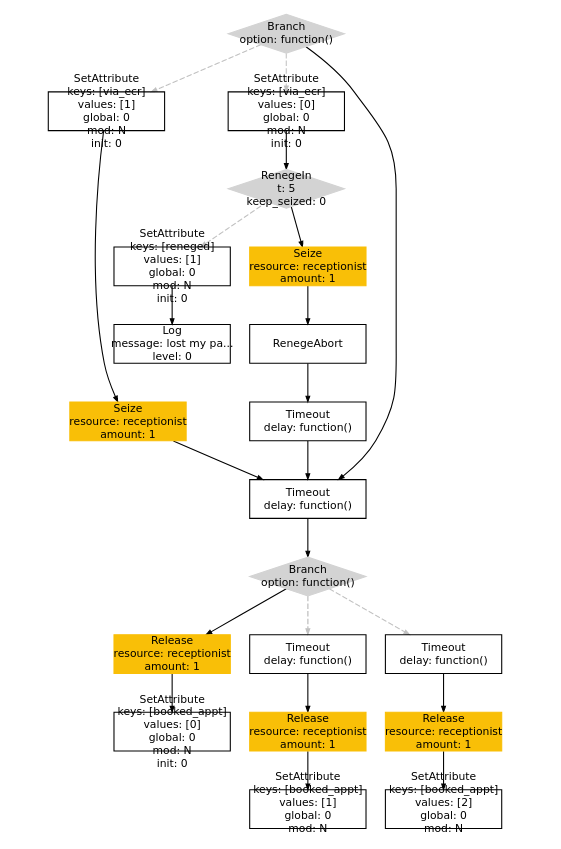
\includegraphics{images/simmer_plot.png}

}

\caption[Simmer Plot: credit to Stacey Croft, Anastasiia Zharinova and
Tom Jemmett ]{Simmer Plot: credit to Stacey Croft, Anastasiia Zharinova and
Tom Jemmett \footnotemark{}}

\end{figure}%
\footnotetext{https://the-strategy-unit.github.io/des\_simmer\_workshop/}

\section{GUI Software}\label{gui-software}

\subsection{JaamSim}\label{jaamsim}

JaamSim is quite different from all of the other offerings discussed so
far due to it providing a graphical, drag and drop interface for
simulations.

You can read more, and download the software, on their
\href{https://jaamsim.com/}{website}.

One big benefit of JaamSim, in addition to its lower barrier to entry,
is the ability to visually demonstrate the movement of entities to
stakeholders, as well as generating graphs which update live as the
simulation is run.

\url{https://youtu.be/cwU3-dNI_hY?si=jbKgzdIOZ8_Dz4rp}

\bookmarksetup{startatroot}

\chapter{Further Reading}\label{further-reading}

\section{SimPy Examples}\label{simpy-examples}

\begin{tcolorbox}[enhanced jigsaw, colframe=quarto-callout-warning-color-frame, bottomtitle=1mm, breakable, rightrule=.15mm, coltitle=black, colbacktitle=quarto-callout-warning-color!10!white, opacityback=0, leftrule=.75mm, arc=.35mm, toptitle=1mm, title=\textcolor{quarto-callout-warning-color}{\faExclamationTriangle}\hspace{0.5em}{Warning}, titlerule=0mm, colback=white, toprule=.15mm, bottomrule=.15mm, left=2mm, opacitybacktitle=0.6]

Note that the linked examples will generally not follow the exact
structure we have used throughout this book. However, the fundamental
concepts remain unchanged, and the knowledge you have acquired from this
book should help you to read and understand most simpy models out there.

\end{tcolorbox}

\subsection{General Examples}\label{general-examples}

A list of additional SimPy examples is kept up-to-date
\href{https://github.com/stars/Bergam0t/lists/simpy-examples}{here}.

\subsection{Visualisation Examples}\label{visualisation-examples}

A library of simpy visualisation examples, which may also prove useful
due to containing code for a range of different types of healthcare
model, can be found
\href{https://github.com/Bergam0t/simpy_visualisation}{here}.

\bookmarksetup{startatroot}

\chapter*{References}\label{references}
\addcontentsline{toc}{chapter}{References}

\markboth{References}{References}

\phantomsection\label{refs}
\begin{CSLReferences}{0}{1}
\end{CSLReferences}



\end{document}
